% Options for packages loaded elsewhere
\PassOptionsToPackage{unicode}{hyperref}
\PassOptionsToPackage{hyphens}{url}
\documentclass[
]{article}
\usepackage{xcolor}
\usepackage[margin=1in]{geometry}
\usepackage{amsmath,amssymb}
\setcounter{secnumdepth}{5}
\usepackage{iftex}
\ifPDFTeX
  \usepackage[T1]{fontenc}
  \usepackage[utf8]{inputenc}
  \usepackage{textcomp} % provide euro and other symbols
\else % if luatex or xetex
  \usepackage{unicode-math} % this also loads fontspec
  \defaultfontfeatures{Scale=MatchLowercase}
  \defaultfontfeatures[\rmfamily]{Ligatures=TeX,Scale=1}
\fi
\usepackage{lmodern}
\ifPDFTeX\else
  % xetex/luatex font selection
\fi
% Use upquote if available, for straight quotes in verbatim environments
\IfFileExists{upquote.sty}{\usepackage{upquote}}{}
\IfFileExists{microtype.sty}{% use microtype if available
  \usepackage[]{microtype}
  \UseMicrotypeSet[protrusion]{basicmath} % disable protrusion for tt fonts
}{}
\makeatletter
\@ifundefined{KOMAClassName}{% if non-KOMA class
  \IfFileExists{parskip.sty}{%
    \usepackage{parskip}
  }{% else
    \setlength{\parindent}{0pt}
    \setlength{\parskip}{6pt plus 2pt minus 1pt}}
}{% if KOMA class
  \KOMAoptions{parskip=half}}
\makeatother
\usepackage{color}
\usepackage{fancyvrb}
\newcommand{\VerbBar}{|}
\newcommand{\VERB}{\Verb[commandchars=\\\{\}]}
\DefineVerbatimEnvironment{Highlighting}{Verbatim}{commandchars=\\\{\}}
% Add ',fontsize=\small' for more characters per line
\usepackage{framed}
\definecolor{shadecolor}{RGB}{248,248,248}
\newenvironment{Shaded}{\begin{snugshade}}{\end{snugshade}}
\newcommand{\AlertTok}[1]{\textcolor[rgb]{0.94,0.16,0.16}{#1}}
\newcommand{\AnnotationTok}[1]{\textcolor[rgb]{0.56,0.35,0.01}{\textbf{\textit{#1}}}}
\newcommand{\AttributeTok}[1]{\textcolor[rgb]{0.13,0.29,0.53}{#1}}
\newcommand{\BaseNTok}[1]{\textcolor[rgb]{0.00,0.00,0.81}{#1}}
\newcommand{\BuiltInTok}[1]{#1}
\newcommand{\CharTok}[1]{\textcolor[rgb]{0.31,0.60,0.02}{#1}}
\newcommand{\CommentTok}[1]{\textcolor[rgb]{0.56,0.35,0.01}{\textit{#1}}}
\newcommand{\CommentVarTok}[1]{\textcolor[rgb]{0.56,0.35,0.01}{\textbf{\textit{#1}}}}
\newcommand{\ConstantTok}[1]{\textcolor[rgb]{0.56,0.35,0.01}{#1}}
\newcommand{\ControlFlowTok}[1]{\textcolor[rgb]{0.13,0.29,0.53}{\textbf{#1}}}
\newcommand{\DataTypeTok}[1]{\textcolor[rgb]{0.13,0.29,0.53}{#1}}
\newcommand{\DecValTok}[1]{\textcolor[rgb]{0.00,0.00,0.81}{#1}}
\newcommand{\DocumentationTok}[1]{\textcolor[rgb]{0.56,0.35,0.01}{\textbf{\textit{#1}}}}
\newcommand{\ErrorTok}[1]{\textcolor[rgb]{0.64,0.00,0.00}{\textbf{#1}}}
\newcommand{\ExtensionTok}[1]{#1}
\newcommand{\FloatTok}[1]{\textcolor[rgb]{0.00,0.00,0.81}{#1}}
\newcommand{\FunctionTok}[1]{\textcolor[rgb]{0.13,0.29,0.53}{\textbf{#1}}}
\newcommand{\ImportTok}[1]{#1}
\newcommand{\InformationTok}[1]{\textcolor[rgb]{0.56,0.35,0.01}{\textbf{\textit{#1}}}}
\newcommand{\KeywordTok}[1]{\textcolor[rgb]{0.13,0.29,0.53}{\textbf{#1}}}
\newcommand{\NormalTok}[1]{#1}
\newcommand{\OperatorTok}[1]{\textcolor[rgb]{0.81,0.36,0.00}{\textbf{#1}}}
\newcommand{\OtherTok}[1]{\textcolor[rgb]{0.56,0.35,0.01}{#1}}
\newcommand{\PreprocessorTok}[1]{\textcolor[rgb]{0.56,0.35,0.01}{\textit{#1}}}
\newcommand{\RegionMarkerTok}[1]{#1}
\newcommand{\SpecialCharTok}[1]{\textcolor[rgb]{0.81,0.36,0.00}{\textbf{#1}}}
\newcommand{\SpecialStringTok}[1]{\textcolor[rgb]{0.31,0.60,0.02}{#1}}
\newcommand{\StringTok}[1]{\textcolor[rgb]{0.31,0.60,0.02}{#1}}
\newcommand{\VariableTok}[1]{\textcolor[rgb]{0.00,0.00,0.00}{#1}}
\newcommand{\VerbatimStringTok}[1]{\textcolor[rgb]{0.31,0.60,0.02}{#1}}
\newcommand{\WarningTok}[1]{\textcolor[rgb]{0.56,0.35,0.01}{\textbf{\textit{#1}}}}
\usepackage{longtable,booktabs,array}
\usepackage{calc} % for calculating minipage widths
% Correct order of tables after \paragraph or \subparagraph
\usepackage{etoolbox}
\makeatletter
\patchcmd\longtable{\par}{\if@noskipsec\mbox{}\fi\par}{}{}
\makeatother
% Allow footnotes in longtable head/foot
\IfFileExists{footnotehyper.sty}{\usepackage{footnotehyper}}{\usepackage{footnote}}
\makesavenoteenv{longtable}
\usepackage{graphicx}
\makeatletter
\newsavebox\pandoc@box
\newcommand*\pandocbounded[1]{% scales image to fit in text height/width
  \sbox\pandoc@box{#1}%
  \Gscale@div\@tempa{\textheight}{\dimexpr\ht\pandoc@box+\dp\pandoc@box\relax}%
  \Gscale@div\@tempb{\linewidth}{\wd\pandoc@box}%
  \ifdim\@tempb\p@<\@tempa\p@\let\@tempa\@tempb\fi% select the smaller of both
  \ifdim\@tempa\p@<\p@\scalebox{\@tempa}{\usebox\pandoc@box}%
  \else\usebox{\pandoc@box}%
  \fi%
}
% Set default figure placement to htbp
\def\fps@figure{htbp}
\makeatother
% definitions for citeproc citations
\NewDocumentCommand\citeproctext{}{}
\NewDocumentCommand\citeproc{mm}{%
  \begingroup\def\citeproctext{#2}\cite{#1}\endgroup}
\makeatletter
 % allow citations to break across lines
 \let\@cite@ofmt\@firstofone
 % avoid brackets around text for \cite:
 \def\@biblabel#1{}
 \def\@cite#1#2{{#1\if@tempswa , #2\fi}}
\makeatother
\newlength{\cslhangindent}
\setlength{\cslhangindent}{1.5em}
\newlength{\csllabelwidth}
\setlength{\csllabelwidth}{3em}
\newenvironment{CSLReferences}[2] % #1 hanging-indent, #2 entry-spacing
 {\begin{list}{}{%
  \setlength{\itemindent}{0pt}
  \setlength{\leftmargin}{0pt}
  \setlength{\parsep}{0pt}
  % turn on hanging indent if param 1 is 1
  \ifodd #1
   \setlength{\leftmargin}{\cslhangindent}
   \setlength{\itemindent}{-1\cslhangindent}
  \fi
  % set entry spacing
  \setlength{\itemsep}{#2\baselineskip}}}
 {\end{list}}
\usepackage{calc}
\newcommand{\CSLBlock}[1]{\hfill\break\parbox[t]{\linewidth}{\strut\ignorespaces#1\strut}}
\newcommand{\CSLLeftMargin}[1]{\parbox[t]{\csllabelwidth}{\strut#1\strut}}
\newcommand{\CSLRightInline}[1]{\parbox[t]{\linewidth - \csllabelwidth}{\strut#1\strut}}
\newcommand{\CSLIndent}[1]{\hspace{\cslhangindent}#1}
\setlength{\emergencystretch}{3em} % prevent overfull lines
\providecommand{\tightlist}{%
  \setlength{\itemsep}{0pt}\setlength{\parskip}{0pt}}
\usepackage{booktabs}
\usepackage{longtable}
\usepackage{array}
\usepackage{multirow}
\usepackage{wrapfig}
\usepackage{float}
\usepackage{colortbl}
\usepackage{pdflscape}
\usepackage{tabu}
\usepackage{threeparttable}
\usepackage{threeparttablex}
\usepackage[normalem]{ulem}
\usepackage{makecell}
\usepackage{xcolor}
\usepackage{bookmark}
\IfFileExists{xurl.sty}{\usepackage{xurl}}{} % add URL line breaks if available
\urlstyle{same}
\hypersetup{
  pdftitle={Curso de Inferência Causal},
  pdfauthor={Manoel Galdino},
  hidelinks,
  pdfcreator={LaTeX via pandoc}}

\title{Curso de Inferência Causal}
\author{Manoel Galdino}
\date{2026-06-11}

\begin{document}
\maketitle

{
\setcounter{tocdepth}{2}
\tableofcontents
}
\section{Introdução}\label{introduuxe7uxe3o}

Escolas que recebem mais recursos financeiros produzem melhores resultados educacionais? Municípios governados por prefeitos reeleitos são mais ou menos corruptos? Programas de transferência de renda reduzem a pobreza? Se olharmos os dados, frequentemente encontramos correlações que sugerem respostas --- mas correlação não é causalidade. O desafio central da inferência causal é justamente ir além da associação estatística e identificar relações de causa e efeito a partir de dados observacionais ou experimentais.

Este curso apresenta os principais métodos de inferência causal utilizados em Ciência Política e áreas afins. Começamos pelo modelo de resultados potenciais (\emph{potential outcomes}) e por grafos acíclicos direcionados (DAGs), que fornecem os fundamentos teóricos. Em seguida, estudamos os principais desenhos de pesquisa: experimentos aleatorizados, \emph{matching}, variáveis instrumentais, regressão descontínua e diferenças em diferenças. Ao longo do curso, também discutimos controle sintético, dados em painel, aprendizado de máquina para inferência causal e outros tópicos avançados.

\subsection{A revolução da credibilidade em ciência política}\label{a-revoluuxe7uxe3o-da-credibilidade-em-ciuxeancia-poluxedtica}

Nas últimas duas décadas, a ciência política passou por uma transformação metodológica conhecida como \emph{revolução da credibilidade} (Angrist e Pischke, 2010). Essa revolução consiste em uma mudança de abordagem na pesquisa empírica quantitativa: de estratégias \emph{model-based} para estratégias \emph{design-based}.

\textbf{Abordagens \emph{model-based}} identificam efeitos causais por meio de suposições de modelagem estatística --- como linearidade, independência condicional e forma funcional --- frequentemente interpretando coeficientes de regressão como causais sem articular explicitamente um desenho de pesquisa ou uma estratégia de identificação separada da especificação do modelo. Um exemplo típico é incluir muitas variáveis de controle em uma regressão na esperança de eliminar viés de variável omitida, sem justificar por que aquele conjunto de controles é suficiente.

\textbf{Abordagens \emph{design-based}} identificam efeitos causais explorando uma fonte de variação exógena na atribuição do tratamento --- como aleatorização, regras institucionais, descontinuidades ou choques --- e declaram explicitamente as suposições de identificação necessárias (ignorabilidade, tendências paralelas, continuidade, restrição de exclusão). A credibilidade da estimativa vem do \emph{desenho de pesquisa}, não da especificação do modelo.

Um estudo recente de Torreblanca et al.~(2026) quantificou o alcance dessa revolução, classificando 91.632 artigos publicados entre 2003 e 2023 em 174 periódicos de ciência política. A Figura 1 mostra a classificação sequencial desses artigos: do total, 41\% são empíricos quantitativos; destes, a grande maioria (81\%) busca explicar relações causais; e dentro dos estudos explanatórios, os métodos \emph{design-based} e \emph{model-based} disputam espaço quase que em paridade.

\begin{figure}
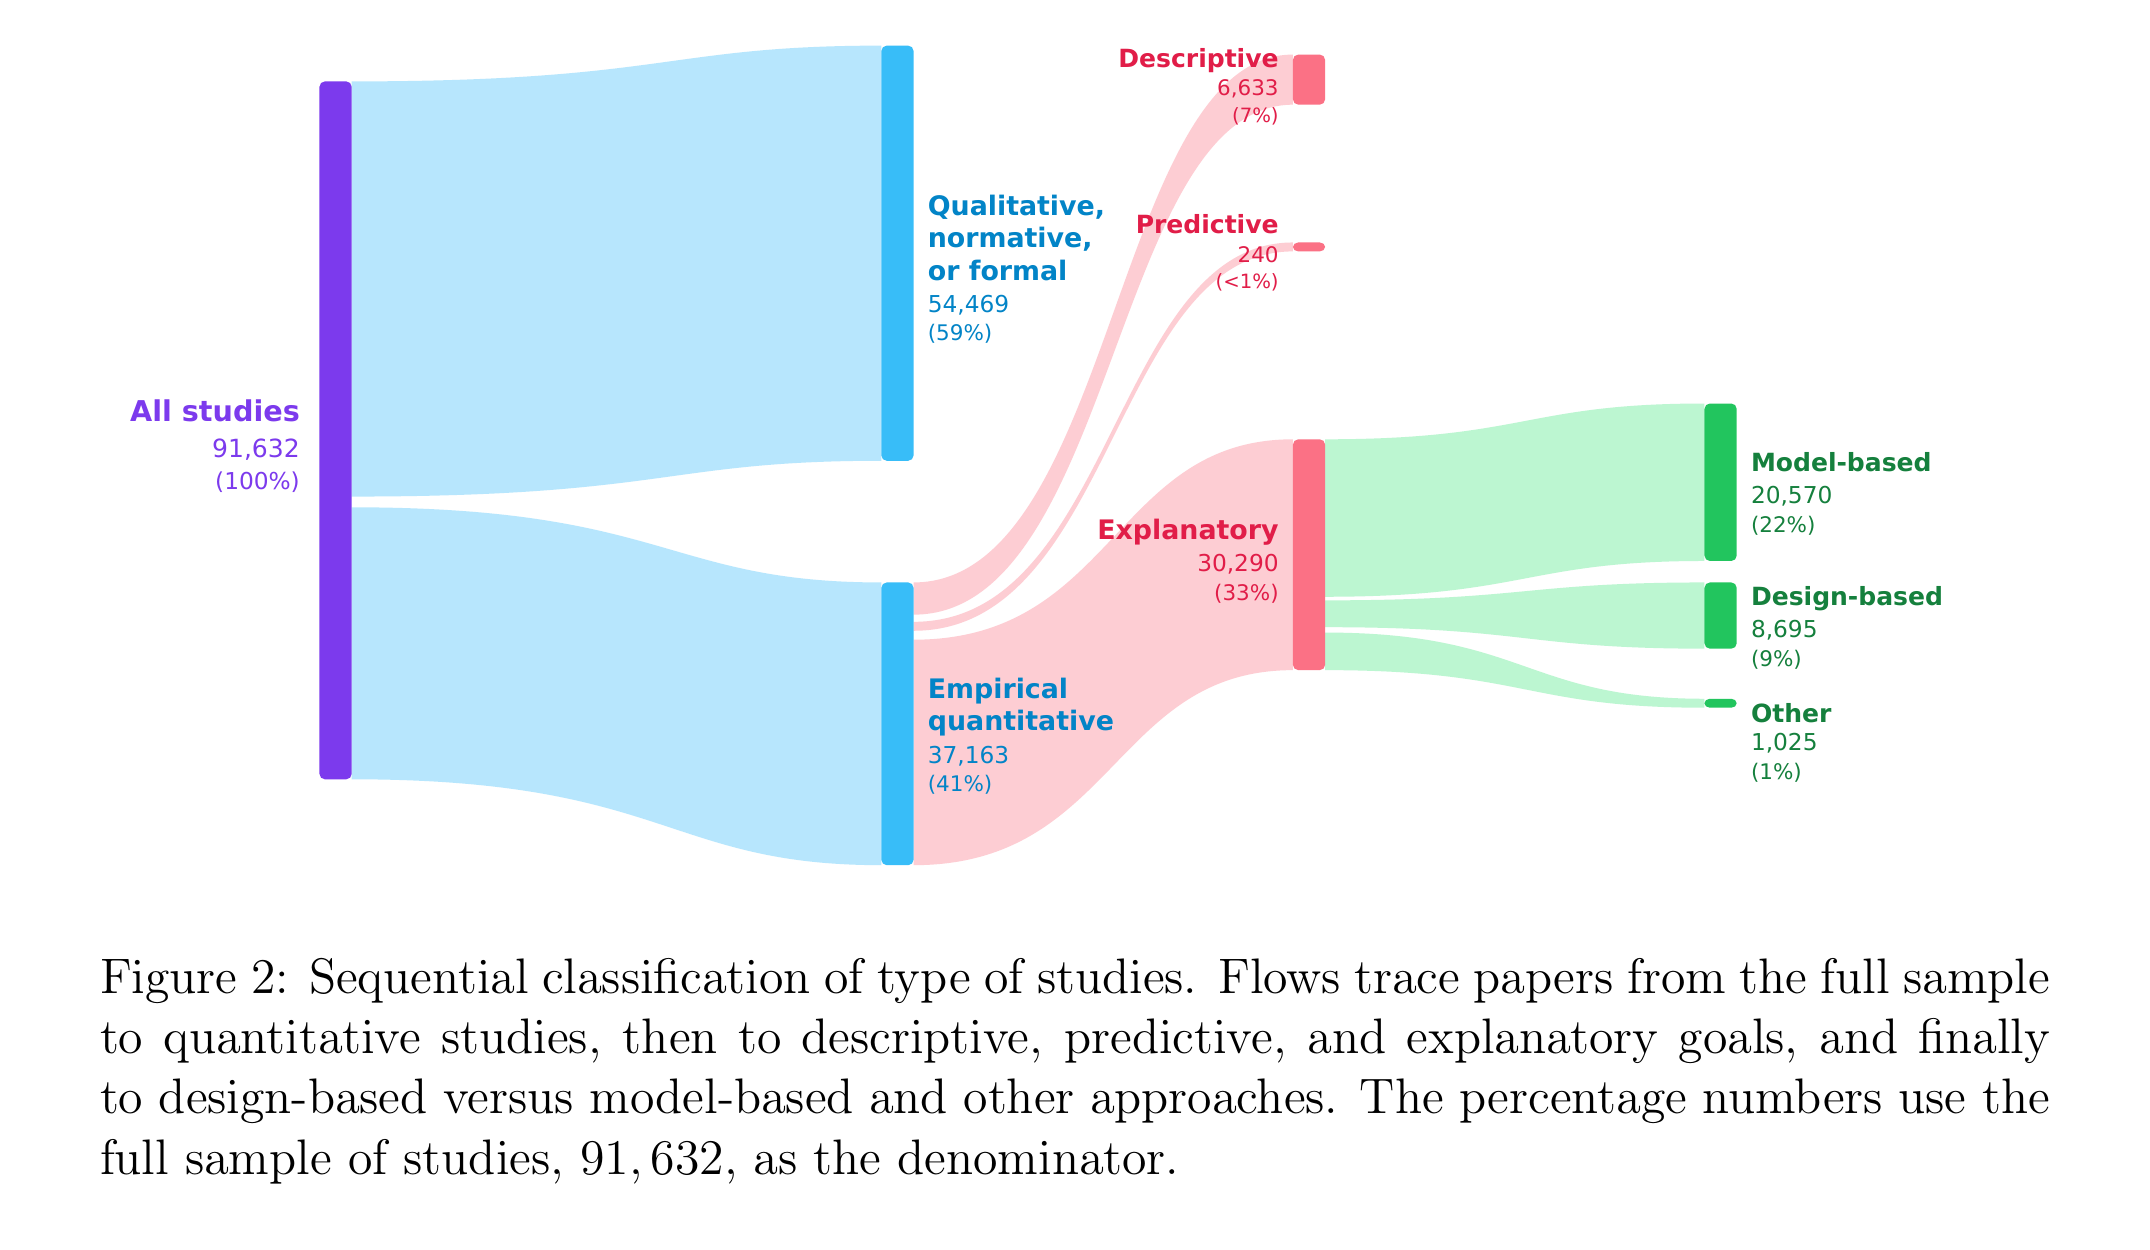
\includegraphics[width=0.9\linewidth]{figures/fig2_classificacao} \caption{Classifica<U+00E7><U+00E3>o sequencial dos tipos de estudos em ci<U+00EA>ncia pol<U+00ED>tica. Dos 91.632 artigos, o fluxo vai de todos os estudos para quantitativos, depois para descritivos, preditivos e explanat<U+00F3>rios, e finalmente para design-based vs. model-based. Fonte: Torreblanca et al. (2026).}\label{fig:fig-classificacao}
\end{figure}

A Figura 2 detalha a evolução temporal dos diferentes métodos \emph{design-based} entre os estudos explanatórios. Experimentos survey são o principal motor do crescimento, seguidos por diferenças em diferenças e matching. Variáveis instrumentais, regressão descontínua, experimentos de campo e controle sintético mantêm participações menores, mas estáveis ou em crescimento modesto.

\begin{figure}
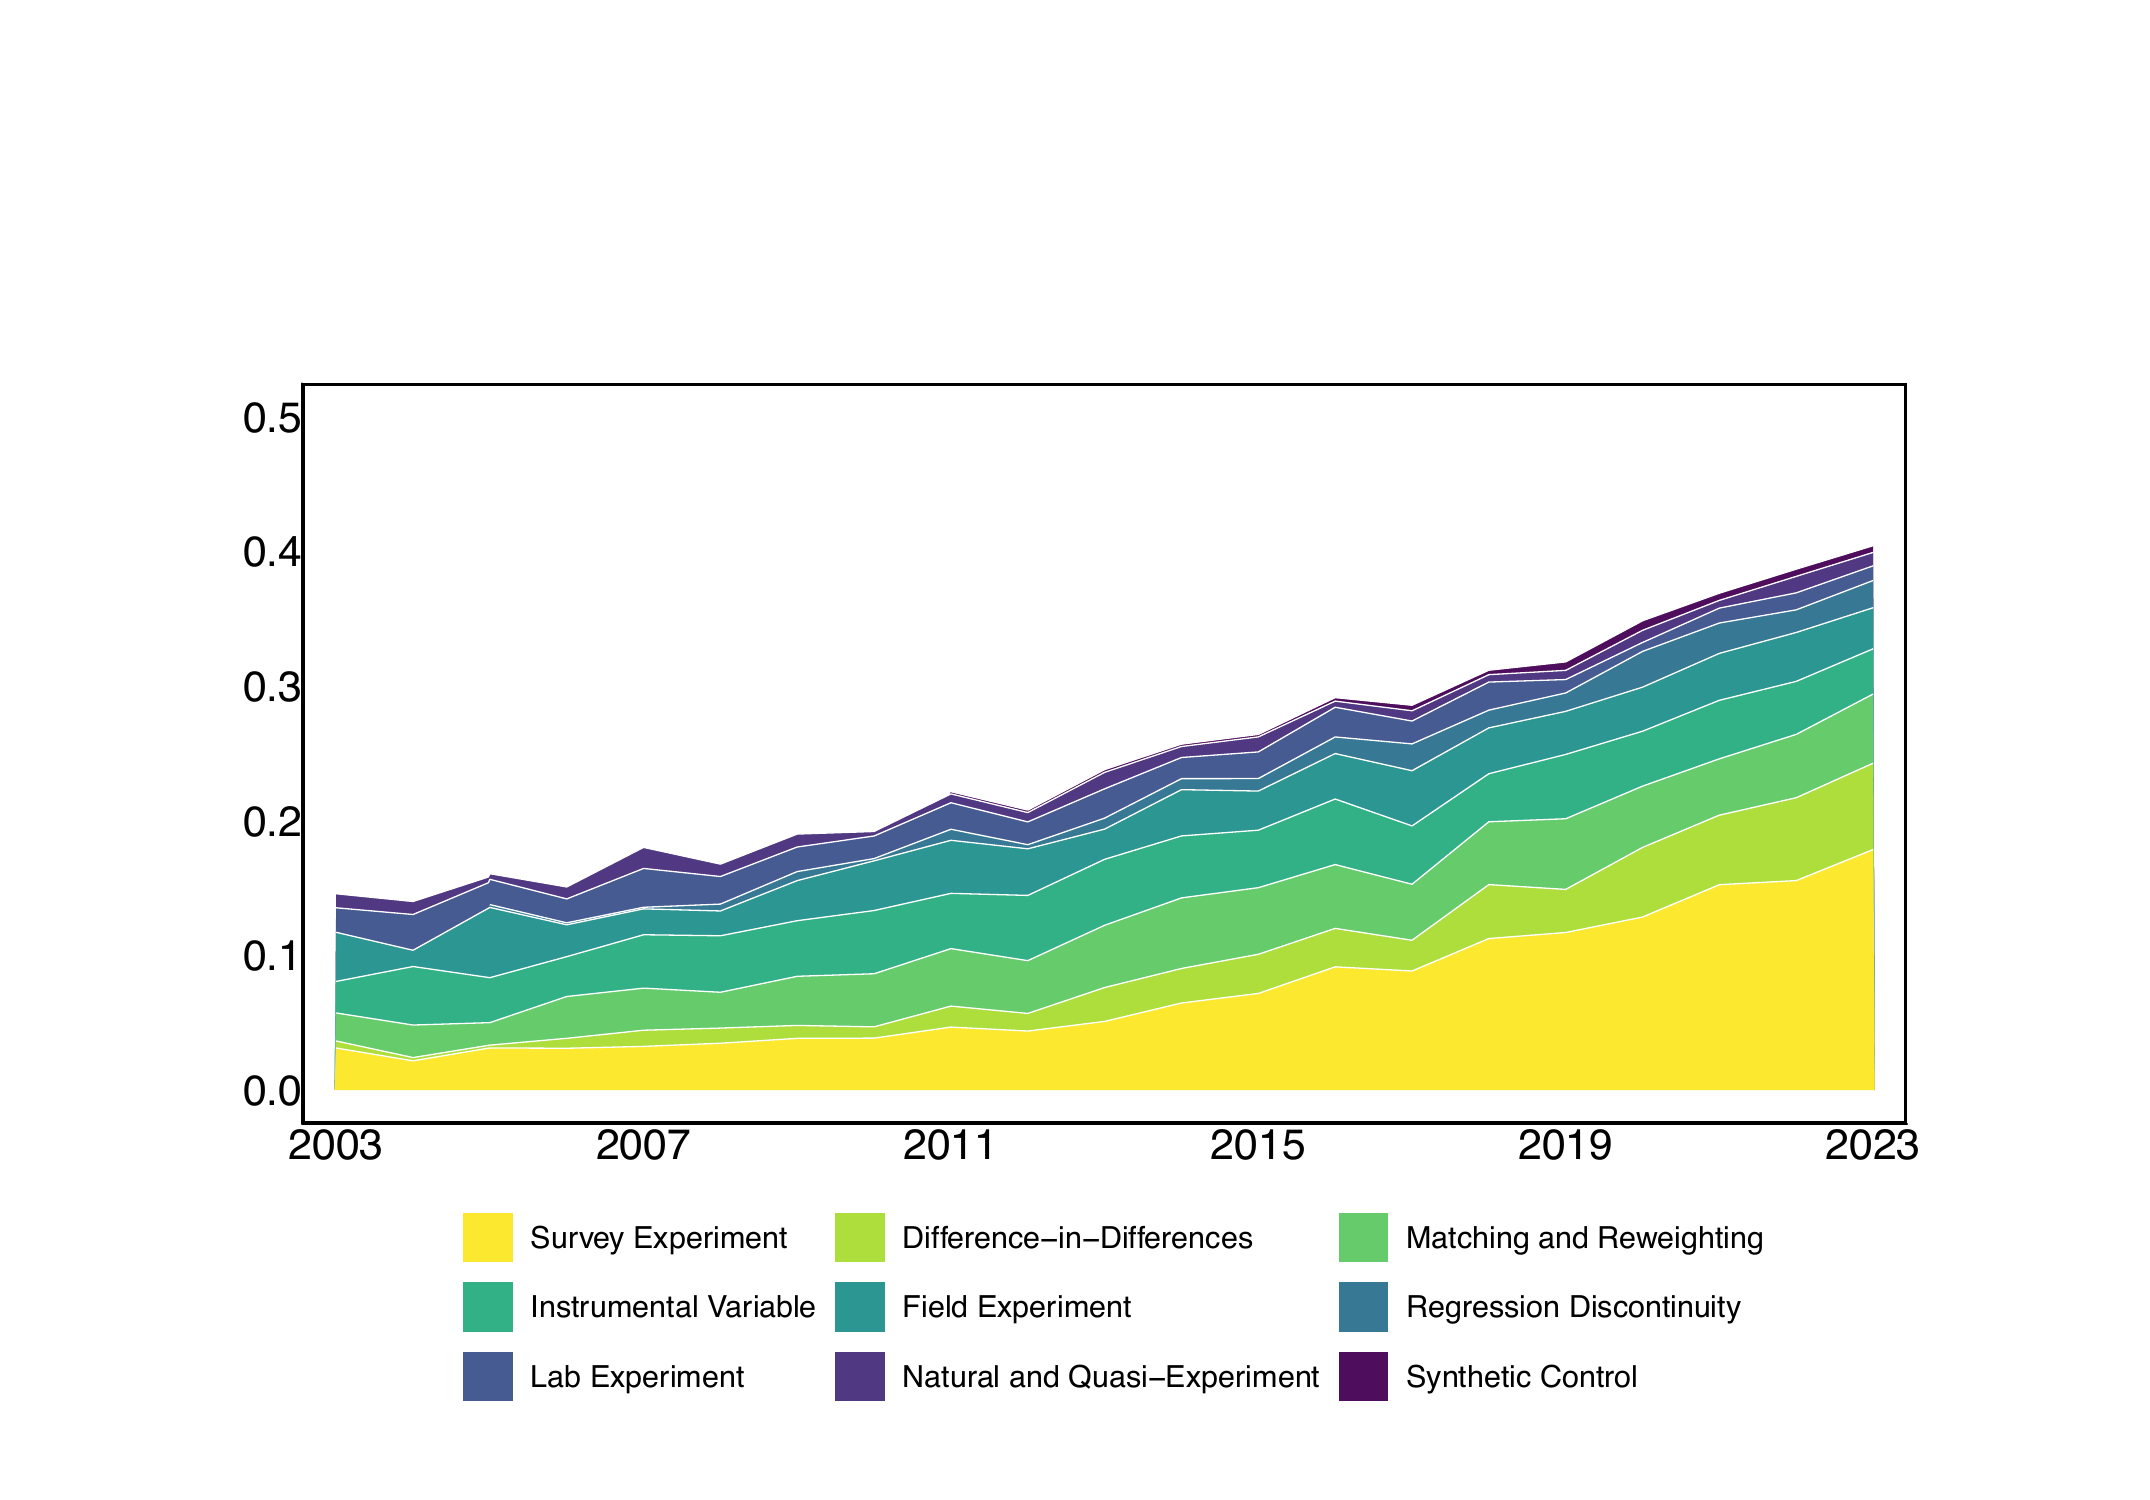
\includegraphics[width=0.9\linewidth]{figures/fig5_metodos} \caption{Propor<U+00E7><U+00E3>o de cada m<U+00E9>todo design-based entre os estudos explanat<U+00F3>rios quantitativos, por ano (2003<U+2013>2023). Fonte: Torreblanca et al. (2026).}\label{fig:fig-metodos}
\end{figure}

Esses dados mostram que os métodos que estudaremos neste curso --- experimentos (Caps. 3--4), matching (Cap. 6), variáveis instrumentais (Cap. 7), diferenças em diferenças (Cap. 8), regressão descontínua (Cap. 9) e controle sintético (Cap. 11) --- correspondem exatamente às ferramentas que transformaram a prática da inferência causal na disciplina. A revolução é real, embora parcial e desigual: ainda em 2023, cerca de 40\% dos estudos explanatórios não empregam uma estratégia de identificação explícita.

Mas por que começar com uma revisão de regressão? Porque a regressão é a ferramenta estatística mais utilizada nas ciências sociais --- e muitos dos métodos causais que estudaremos são implementados por meio de alguma forma de regressão. Compreender bem o que a regressão faz (e o que ela \emph{não} faz) é essencial para entender quando ela pode ser interpretada causalmente e quando não pode.

\subsection{Revisão de Regressão}\label{revisuxe3o-de-regressuxe3o}

Comecemos pelo modelo de regressão populacional dado por:
\[y = \beta_0 + \beta_1 x + u\]

As suposições básicas do modelo são:

\begin{enumerate}
\def\labelenumi{\arabic{enumi}.}
\item
  Média do erro é zero (sem perda de generalidade): \(\mathbb{E}[u] = 0\)
\item
  Independência na média do erro: \(\mathbb{E}[u|x] = \mathbb{E}[u]\). Essa é a suposição mais consequente do modelo de regressão. Como é sobre o termo de erro, não é testável. Um exemplo é útil para entender o que significa essa suposição. Suponha que estamos interessados no efeito do gasto de campanha (\(x\)) sobre o voto (\(y\)). O termo de erro \(u\) seria a qualidade da candidata, não observável. A suposição implica então que a qualidade média das candidatas que gastam 100 mil reais é a mesma das que gastam 500 mil e um milhão (e assim por diante). Se candidatas melhores arrecadam mais dinheiro e, portanto, gastam mais, a suposição foi violada.
\end{enumerate}

Conectando 1 e 2, temos: \(\mathbb{E}[u|x] = 0\). Essa suposição é chamada de ``média condicional zero'' ou ``esperança condicional zero'' do termo de erro. Ela implica que:
\(\mathbb{E}[y|x] = \beta_0 + \beta_1 x\). Essa equação é chamada de Conditional Expectation Function, ou CEF.

De posse de uma amostra aleatória simples, podemos derivar os estimadores de mínimos quadrados (MQO ou OLS na sigla em inglês). Vou pular os passos da derivação. Para nós, o importante é lembrar a fórmula do \(\hat{\beta}_1\):

\(\hat{\beta}_1 = \frac{\text{covariância amostral}}{\text{variância amostral}} = \frac{\sum_{i=1}^n(x_i - \bar{x})(y_i - \bar{y})}{\sum_{i=1}^n(x_i - \bar{x})^2}\)

E \(\hat{\beta}_0 = \bar{y} - \hat{\beta}_1\bar{x}\).

Podemos então demonstrar que o estimador é não-viesado. Para isso, é necessário supor que o modelo é linear nos parâmetros (não nas variáveis), temos uma amostra aleatória simples da população, existe variância no preditor (para não dividir por zero na fórmula do estimador de OLS) e a média condicional zero. Para a derivação completa dos estimadores e a demonstração de não-viés, ver Wooldridge (2013, cap. 2).

\subsubsection{Teorema da Anatomia da Regressão}\label{teorema-da-anatomia-da-regressuxe3o}

Na prática, raramente rodamos uma regressão com um único preditor. O que acontece quando adicionamos variáveis de controle a uma regressão? Como o coeficiente de uma variável muda quando ``controlamos'' por outras? O Teorema da Anatomia da Regressão nos dá uma resposta precisa a essas perguntas.

Esse teorema, também conhecido como teorema de Frisch-Waugh-Lovell (FWL), é fundamental para entender regressão múltipla e, como veremos ao longo do curso, para entender o que vários métodos causais fazem ``por debaixo dos panos''.

\textbf{Enunciado.} Suponha que nosso modelo possui \(2\) preditores:

\[y_i=\beta_0+\beta_1 x_{1i}+ \beta_2 x_{2i}+ e_i\]

E rodamos uma regressão auxiliar de \(x_1\) sobre \(x_2\):

\[x_{1i}=\gamma_0+\gamma_{1}x_{2i} + f_i\]

com resíduos \(\tilde{x}_{1i}=x_{1i} - \hat{\gamma}_0 - \hat{\gamma}_1 x_{2i}\). Esses resíduos representam a parte da variação de \(x_1\) que \emph{não} é explicada por \(x_2\).

O Teorema FWL afirma que o coeficiente \(\hat{\beta}_1\) da regressão múltipla é \emph{idêntico} ao coeficiente obtido regredindo \(y\) sobre \(\tilde{x}_1\):

\[\hat{\beta}_1 = \frac{\sum_{i=1}^n \tilde{x}_{1i}\, y_i}{\sum_{i=1}^n \tilde{x}_{1i}^2}\]

\textbf{Derivação.} A prova usa duas propriedades básicas dos resíduos de MQO: (i) a soma dos resíduos é zero, \(\sum \tilde{x}_{1i} = 0\); e (ii) os resíduos são ortogonais aos regressores, \(\sum \tilde{x}_{1i}\, x_{2i} = 0\).

Partimos do fato de que os resíduos \(\hat{e}_i = y_i - \hat{\beta}_0 - \hat{\beta}_1 x_{1i} - \hat{\beta}_2 x_{2i}\) da regressão múltipla são ortogonais a qualquer combinação linear dos regressores. Como \(\tilde{x}_{1i} = x_{1i} - \hat{\gamma}_0 - \hat{\gamma}_1 x_{2i}\) é uma combinação linear de \(1\), \(x_{1i}\) e \(x_{2i}\), temos \(\sum \tilde{x}_{1i}\, \hat{e}_i = 0\). Expandindo:

\[\sum_{i=1}^n \tilde{x}_{1i}\left(y_i - \hat{\beta}_0 - \hat{\beta}_1 x_{1i} - \hat{\beta}_2 x_{2i}\right) = 0\]

\[\sum \tilde{x}_{1i}\, y_i = \hat{\beta}_0 \underbrace{\sum \tilde{x}_{1i}}_{=\,0} + \hat{\beta}_1 \sum \tilde{x}_{1i}\, x_{1i} + \hat{\beta}_2 \underbrace{\sum \tilde{x}_{1i}\, x_{2i}}_{=\,0}\]

Resta simplificar \(\sum \tilde{x}_{1i}\, x_{1i}\). Substituindo \(x_{1i} = \tilde{x}_{1i} + \hat{\gamma}_0 + \hat{\gamma}_1 x_{2i}\):

\[\sum \tilde{x}_{1i}\, x_{1i} = \sum \tilde{x}_{1i}^2 + \hat{\gamma}_0 \underbrace{\sum \tilde{x}_{1i}}_{=\,0} + \hat{\gamma}_1 \underbrace{\sum \tilde{x}_{1i}\, x_{2i}}_{=\,0} = \sum \tilde{x}_{1i}^2\]

Portanto:

\[\sum \tilde{x}_{1i}\, y_i = \hat{\beta}_1 \sum \tilde{x}_{1i}^2 \quad \Longrightarrow \quad \hat{\beta}_1 = \frac{\sum \tilde{x}_{1i}\, y_i}{\sum \tilde{x}_{1i}^2} \qquad \blacksquare\]

\textbf{Intuição.} O teorema nos diz que ``controlar por \(x_2\)'' em uma regressão múltipla equivale a dois passos: primeiro, remover de \(x_1\) tudo o que \(x_2\) consegue explicar; depois, regredir \(y\) sobre a variação residual de \(x_1\). Em outras palavras, \(\hat{\beta}_1\) captura a relação entre \(y\) e a parte de \(x_1\) que é \emph{ortogonal} (não correlacionada) a \(x_2\). Essa é a essência do que significa ``controlar por'' uma variável.

Esse resultado generaliza para qualquer número de controles: se tivermos \(k\) variáveis de controle, basta regredir \(x_1\) sobre todas elas, obter os resíduos, e regredir \(y\) sobre esses resíduos.

Vamos visualizar essa relação com um exemplo do livro do Scott Cunningham:

\begin{Shaded}
\begin{Highlighting}[]
\FunctionTok{library}\NormalTok{(tidyverse)}
\FunctionTok{library}\NormalTok{(haven)}

\NormalTok{read\_data }\OtherTok{\textless{}{-}} \ControlFlowTok{function}\NormalTok{(df) \{}
\NormalTok{  full\_path }\OtherTok{\textless{}{-}} \FunctionTok{paste0}\NormalTok{(}\StringTok{"https://github.com/scunning1975/mixtape/raw/master/"}\NormalTok{,}
\NormalTok{                      df)}
\NormalTok{  haven}\SpecialCharTok{::}\FunctionTok{read\_dta}\NormalTok{(full\_path)}
\NormalTok{\}}

\NormalTok{auto }\OtherTok{\textless{}{-}}
  \FunctionTok{read\_data}\NormalTok{(}\StringTok{"auto.dta"}\NormalTok{) }\SpecialCharTok{\%\textgreater{}\%}
  \FunctionTok{mutate}\NormalTok{(}\AttributeTok{length =}\NormalTok{ length }\SpecialCharTok{{-}} \FunctionTok{mean}\NormalTok{(length))}

\NormalTok{lm1 }\OtherTok{\textless{}{-}} \FunctionTok{lm}\NormalTok{(price }\SpecialCharTok{\textasciitilde{}}\NormalTok{ length, auto)}
\NormalTok{lm2 }\OtherTok{\textless{}{-}} \FunctionTok{lm}\NormalTok{(price }\SpecialCharTok{\textasciitilde{}}\NormalTok{ length }\SpecialCharTok{+}\NormalTok{ weight }\SpecialCharTok{+}\NormalTok{ headroom }\SpecialCharTok{+}\NormalTok{ mpg, auto)}
\NormalTok{lm\_aux }\OtherTok{\textless{}{-}} \FunctionTok{lm}\NormalTok{(length }\SpecialCharTok{\textasciitilde{}}\NormalTok{ weight }\SpecialCharTok{+}\NormalTok{ headroom }\SpecialCharTok{+}\NormalTok{ mpg, auto)}
\NormalTok{auto }\OtherTok{\textless{}{-}}
\NormalTok{  auto }\SpecialCharTok{\%\textgreater{}\%}
  \FunctionTok{mutate}\NormalTok{(}\AttributeTok{length\_resid =} \FunctionTok{residuals}\NormalTok{(lm\_aux))}

\NormalTok{lm2\_alt }\OtherTok{\textless{}{-}} \FunctionTok{lm}\NormalTok{(price }\SpecialCharTok{\textasciitilde{}}\NormalTok{ length\_resid, auto)}

\NormalTok{coef\_lm1 }\OtherTok{\textless{}{-}}\NormalTok{ lm1}\SpecialCharTok{$}\NormalTok{coefficients}
\NormalTok{coef\_lm2\_alt }\OtherTok{\textless{}{-}}\NormalTok{ lm2\_alt}\SpecialCharTok{$}\NormalTok{coefficients}

\NormalTok{y\_single }\OtherTok{\textless{}{-}} \FunctionTok{tibble}\NormalTok{(}\AttributeTok{price =}\NormalTok{ coef\_lm2\_alt[}\DecValTok{1}\NormalTok{] }\SpecialCharTok{+}\NormalTok{ coef\_lm1[}\DecValTok{2}\NormalTok{]}\SpecialCharTok{*}\NormalTok{auto}\SpecialCharTok{$}\NormalTok{length\_resid,}
                   \AttributeTok{length\_resid =}\NormalTok{ auto}\SpecialCharTok{$}\NormalTok{length\_resid)}

\NormalTok{y\_multi }\OtherTok{\textless{}{-}} \FunctionTok{tibble}\NormalTok{(}\AttributeTok{price =}\NormalTok{ coef\_lm2\_alt[}\DecValTok{1}\NormalTok{] }\SpecialCharTok{+}\NormalTok{ coef\_lm2\_alt[}\DecValTok{2}\NormalTok{]}\SpecialCharTok{*}\NormalTok{auto}\SpecialCharTok{$}\NormalTok{length\_resid,}
                  \AttributeTok{length\_resid =}\NormalTok{ auto}\SpecialCharTok{$}\NormalTok{length\_resid)}

\NormalTok{auto }\SpecialCharTok{\%\textgreater{}\%}
  \FunctionTok{ggplot}\NormalTok{(}\FunctionTok{aes}\NormalTok{(}\AttributeTok{x=}\NormalTok{length\_resid, }\AttributeTok{y =}\NormalTok{ price)) }\SpecialCharTok{+}
  \FunctionTok{geom\_point}\NormalTok{() }\SpecialCharTok{+}
  \FunctionTok{geom\_smooth}\NormalTok{(}\AttributeTok{data =}\NormalTok{ y\_multi, }\AttributeTok{color =} \StringTok{"blue"}\NormalTok{) }\SpecialCharTok{+}
  \FunctionTok{geom\_smooth}\NormalTok{(}\AttributeTok{data =}\NormalTok{ y\_single, }\AttributeTok{color =} \StringTok{"red"}\NormalTok{)}
\end{Highlighting}
\end{Shaded}

\pandocbounded{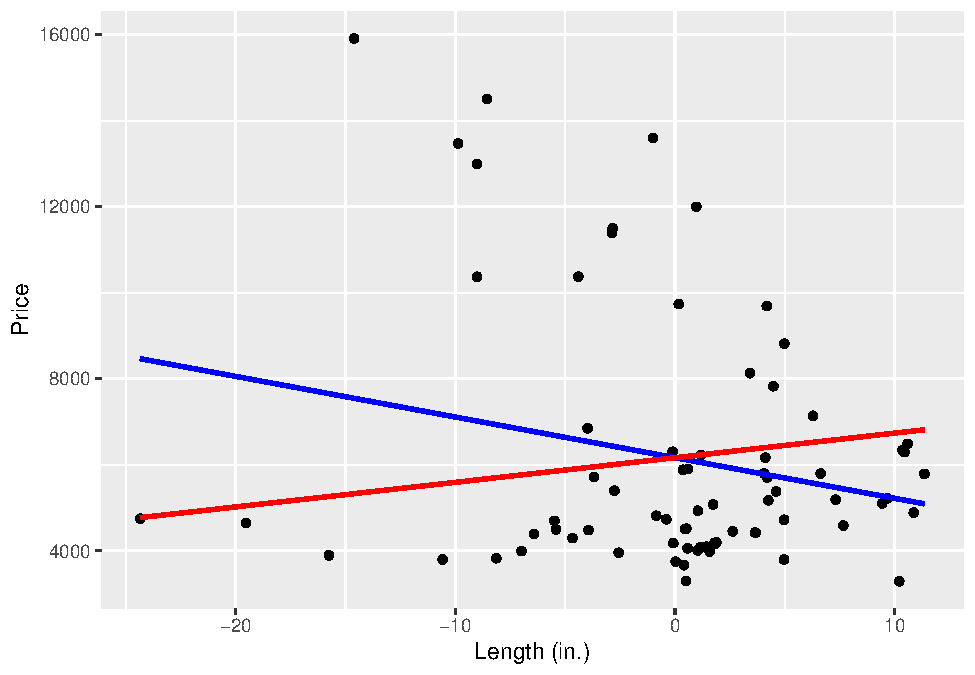
\includegraphics[keepaspectratio]{bookdownproj_files/figure-latex/unnamed-chunk-1-1.pdf}}

O gráfico mostra o preço do carro contra o resíduo de \emph{length} após controlar por \emph{weight}, \emph{headroom} e \emph{mpg}. A linha azul é o coeficiente da regressão múltipla (que, pelo Teorema FWL, é idêntico ao da regressão de \emph{price} sobre \emph{length\_resid}). A linha vermelha é o coeficiente da regressão simples de \emph{price} sobre \emph{length}, sem controles. A diferença entre as duas inclinações reflete exatamente o viés que surge quando \emph{length} está correlacionado com as variáveis omitidas: ao controlar por elas, isolamos a variação ``limpa'' de \emph{length} e obtemos uma estimativa diferente.

\subsection{Inferência}\label{inferuxeancia}

Como sabemos, inferência lida com a generalização da amostra para a população e, portanto, com a variabilidade inerente de amostra para amostra. Eu não vou revisar aqui os cálculos para derivar o erro padrão. Quero apenas enfatizar três pontos que não são usualmente abordados em cursos de regressão.

\subsubsection{Generalização amostral vs.~generalização causal}\label{generalizauxe7uxe3o-amostral-vs.-generalizauxe7uxe3o-causal}

Em primeiro lugar, generalização da amostra para a população é diferente de generalização causal, também conhecida como validade externa. Esse ponto foi confundido por muitos autores, em particular o livro conhecido como KKV (King, Keohane e Verba, 1994), e levou muitos pesquisadores a acreditarem que uma regressão possuía maior capacidade de generalização causal do que estudos de caso. Uma regressão (supondo que o erro padrão foi calculado corretamente) permite generalizar as estimativas para uma população. Porém, o que significa falar em generalização quando temos o universo de casos (por exemplo, todos os deputados, ou todos os candidatos, ou todos os municípios)? Quando temos o universo, não é diferente de estudos de caso que possuem todos os casos relevantes e, portanto, a noção de generalização da amostra para a população não se aplica.

Essa distinção nos leva a uma pergunta natural: se temos todos os casos, ainda assim existe incerteza?

\subsubsection{Incerteza com o universo dos casos}\label{incerteza-com-o-universo-dos-casos}

A resposta é sim. Na inferência causal, em particular nesses casos em que temos o universo dos casos, ainda assim há incerteza. O trabalho de Abadie et al.~(2020) discute a ideia de \emph{design-based} inference. Nós vamos explicar no curso em mais detalhes o que é uma pesquisa \emph{design-based} (em oposição a \emph{model-based}), especialmente no Capítulo 2 (Resultados Potenciais). A ideia desse tipo de incerteza (e seu correspondente erro-padrão) é a seguinte. Imagine que estamos interessados em estimar o efeito causal da reeleição de prefeitos sobre a corrupção municipal. Suponha que tenho todos os municípios na amostra. Por fim, suponha que temos um experimento natural de forma que podemos supor que (talvez condicional a algumas variáveis) a reeleição é aleatória. Não há incerteza amostral para a população, mas há incerteza sobre o que aconteceria com a corrupção para os prefeitos reeleitos, caso não fossem reeleitos (e para os que perderam, como seria a corrupção caso fossem reeleitos). Em particular, se acreditamos que a reeleição foi aleatória, então uma nova rodada de amostragem (em um universo alternativo?) produziria outra configuração de prefeitos reeleitos e não reeleitos e alguma variação na estimativa do efeito causal. Isso antecipa nossa discussão sobre causalidade no Capítulo 2, mas o ponto central é que existe incerteza na estimativa do efeito causal que não deriva de variação amostral propriamente, mas da aleatoriedade da intervenção.

Nas palavras dos autores:

``it will be useful to distinguish between descriptive estimands, where uncertainty stems solely from not observing all units in the population of interest, and causal estimands, where the uncertainty stems, at least partially, from unobservability of some of the potential outcome'' (p.~267). Meu ponto é que KKV e cia confundiram incerteza de estimandos descritivos com estimandos causais.

\subsubsection{Validade externa}\label{validade-externa}

O que me leva de volta ao ponto anterior sobre a comparação entre estudos de caso e métodos quantitativos, quando o objetivo é inferência causal. A incerteza inerente é sobre o efeito da intervenção, não sobre variações amostrais. Além disso, em ambos os casos não sabemos (a princípio) se os estudos possuem validade externa, isto é, se os resultados valem para outras populações, no tempo e espaço. É preciso avançar nessa agenda, tanto em métodos quali como quanti. É um problema em aberto e que tem atraído muitas pesquisas novas, que não iremos cobrir no curso (até por desconhecimento meu de boa parte dessa literatura).

\subsection{Resumo e próximos passos}\label{resumo-e-pruxf3ximos-passos}

Neste capítulo introdutório, revisamos quatro pontos fundamentais:

\begin{enumerate}
\def\labelenumi{\arabic{enumi}.}
\item
  \textbf{A revolução da credibilidade}: a ciência política está em transição de estratégias \emph{model-based} para \emph{design-based}, embora essa transformação ainda seja parcial e desigual. Os métodos deste curso correspondem às ferramentas que lideram essa mudança.
\item
  \textbf{A regressão como ponto de partida}: o modelo de regressão por MQO estima a Função de Esperança Condicional (CEF), mas a interpretação causal do coeficiente depende de suposições fortes --- em particular, a média condicional zero do termo de erro.
\item
  \textbf{O Teorema FWL e o papel dos controles}: adicionar variáveis de controle a uma regressão muda o coeficiente estimado porque estamos isolando a variação do preditor que não é explicada pelos controles. Isso é crucial para entender o que ``controlar por \(X\)'' realmente significa.
\item
  \textbf{Incerteza vai além da amostragem}: mesmo quando temos o universo dos casos, há incerteza causal --- ela vem da aleatoriedade da intervenção, não da variação amostral. Essa distinção entre incerteza descritiva e causal é central para o curso.
\end{enumerate}

No próximo capítulo, formalizamos a noção de causalidade por meio do \textbf{modelo de resultados potenciais} (\emph{potential outcomes}), que fornece a linguagem e o arcabouço teórico para definir efeitos causais de forma precisa.

\subsection{Referências}\label{referuxeancias}

Abadie, Alberto, Susan Athey, Guido W. Imbens, and Jeffrey M. Wooldridge. 2020. ``Sampling-Based Versus Design-Based Uncertainty in Regression Analysis.'' Econometrica 88 (0): 265--96.

Angrist, Joshua D., and Jörn-Steffen Pischke. 2009. \emph{Mostly Harmless Econometrics: An Empiricist's Companion}. Princeton University Press.

Angrist, Joshua D., and Jörn-Steffen Pischke. 2010. ``The Credibility Revolution in Empirical Economics: How Better Research Design Is Taking the Con out of Econometrics.'' \emph{Journal of Economic Perspectives} 24 (2): 3--30.

King, Gary, Robert O. Keohane, and Sidney Verba. 1994. \emph{Designing Social Inquiry: Scientific Inference in Qualitative Research}. Princeton University Press.

Torreblanca, Carolina, William Dinneen, Guy Grossman, and Yiqing Xu. 2026. ``The Credibility Revolution in Political Science.'' Working Paper, University of Pennsylvania and Stanford University.

Wooldridge, Jeffrey M. 2013. \emph{Introductory Econometrics: A Modern Approach}. 5th ed.~South-Western Cengage Learning.

\section{Resultados Potenciais}\label{resultados-potenciais}

Durante muito tempo, inferência causal com regressão era caracterizada por recomendações vagas, ad hoc e inconsistências. O debate sobre o efeito causal do cigarro sobre câncer de pulmão é ilustrativo a esse respeito. Durante décadas, pesquisadores enfrentaram dificuldades para diferenciar correlação de causalidade em estudos epidemiológicos sobre tabagismo. Muitos estudos iniciais baseados apenas em correlação eram contestados por não apresentarem mecanismos claros ou critérios objetivos para validar inferências causais. Fisher (\citeproc{ref-fisher1958}{1958}), por exemplo, questionou os resultados iniciais que ligavam o cigarro ao câncer por falta de critérios explícitos para identificar uma relação causal, argumentando que a correlação observada poderia decorrer de fatores confundidores, causalidade reversa ou problemas de mensuração.

A situação mudou gradualmente com contribuições metodológicas importantes, como os critérios de causalidade propostos por Hill (\citeproc{ref-hill1965}{1965}). Os critérios de Bradford Hill ofereceram uma lista explícita e sistemática para avaliar a plausibilidade causal em estudos observacionais:

\begin{enumerate}
\def\labelenumi{\arabic{enumi}.}
\tightlist
\item
  O efeito deveria ser grande
\item
  Reproduzível em estudos independentes
\item
  Possuir uma relação monotônica com ``dose'' (isto é, aumento na dose não pode reduzir o efeito se o efeito é positivo e vice-versa se for negativo)
\item
  Corresponder a um ``experimento natural''
\item
  Comportar-se apropriadamente quando a causa é aplicada, removida e então reinstalada
\item
  Ser consistente com o conhecimento especializado do tema
\item
  Ser, por exemplo, predita por alguma teoria bem estabelecida
\end{enumerate}

Nós temos amplas evidências de que muitas intervenções são causais, mesmo na ausência de qualquer experimento aleatório controlado. Sabemos, por exemplo, que desfibrilação, manobra de Heimlich e uso de paraquedas são eficazes para prevenir mortes (\citeproc{ref-howick2009}{Howick, Glasziou, and Aronson 2009}).

Em um artigo clássico dos primórdios da estatística escrito por Yule (\citeproc{ref-yule1899}{1899}), temos um dos primeiros exemplos de utilização da regressão para estudar o efeito causal de uma política (ajuda sobre pobreza). E a despeito do título do artigo falar em causalidade (``An investigation into the causes of changes in pauperism in England, chiefly during the last two intercensal decades''), a certa altura ele diz, em nota de rodapé, que ``due to'' deve ser lido como ``associated to''. Quase cem anos depois, o grande estatístico Cox afirmaria em um artigo sobre causalidade: ``it is remarkable how relatively little causality is mentioned in the general statistics literature, except in a social science context'' (\citeproc{ref-cox1992}{Cox 1992, 292}).

Um exemplo da perspectiva de que falava Cox: Muthén (\citeproc{ref-muthen1987}{1987}) chegou a afirmar que ``It would be very healthy if more researchers abandon thinking of and using terms such as cause and effect'' (p.~180). Algo ecoado em uma entrevista com um dos líderes da revolução causal desde os anos 70/80, Jamie Robins, que relata que seus papers (em journals de estatística) eram rejeitados por usar linguagem causal (\citeproc{ref-robins2022}{Robins 2022}). Então parece bastante seguro dizer que a sensação geral na estatística até os anos 80 é que não se deveria usar linguagem causal fora de estudos experimentais, isto é, em estudos observacionais.

\subsection{Da intuição comparativa ao modelo formal}\label{da-intuiuxe7uxe3o-comparativa-ao-modelo-formal}

A ideia de causalidade está presente há muito tempo na ciência política, especialmente na tradição de política comparada qualitativa. Os métodos comparativos de Stuart Mill --- como o método da diferença e o método da concordância --- buscam identificar relações causais comparando casos que diferem apenas na presença ou ausência de um fator de interesse. No fundo, essa lógica comparativa já contém o germe do raciocínio contrafactual: perguntar ``o que teria acontecido se este fator estivesse ausente?'' é exatamente o que fazemos ao comparar um caso tratado com um caso de controle.

A moderna forma de pensar causalidade formaliza essa intuição, abandonando o paradigma de relações necessárias e/ou suficientes (que pressupõe determinismo) para adotar um framework probabilístico baseado em resultados potenciais. Essa formalização nos permite definir com precisão o que é um efeito causal, explicitar as suposições que precisamos fazer, e entender quando e por que nossas estimativas podem ser viesadas.

\subsection{\texorpdfstring{Resultados Potenciais (\emph{Potential Outcomes})}{Resultados Potenciais (Potential Outcomes)}}\label{resultados-potenciais-potential-outcomes}

Neste capítulo, formalizamos a ideia de causalidade usando o modelo de resultados potenciais (\emph{potential outcomes}), também conhecido como Modelo Causal de Neyman-Rubin. Esse framework nos dará uma linguagem precisa para definir efeitos causais e explicitar as suposições necessárias para estimá-los.

\textbf{Objetivos de aprendizado:}

\begin{enumerate}
\def\labelenumi{\arabic{enumi}.}
\tightlist
\item
  Compreender a notação de resultados potenciais e a \emph{switching equation}
\item
  Distinguir entre estimando, estimador e estimativa
\item
  Definir os principais estimandos causais: ATE, ATT e CATE
\item
  Enunciar as condições de identificação do ATE (ignorabilidade forte)
\item
  Conectar o modelo de resultados potenciais à regressão linear e interpretar o viés
\end{enumerate}

Vamos começar fixando a notação que utilizaremos ao longo de todo o curso.

\subsection{Notação}\label{notauxe7uxe3o}

Vamos assumir que existe um tratamento binário, que recebe o valor \(1\) se a unidade \(i\) recebe o tratamento, e \(0\) caso contrário, dado por: \(D_i \in \{1,0\}\).

Suponha que tenhamos \(N\) unidades que podem receber o tratamento ou controle. Então, o resultado potencial para a unidade \(i\) é \(Y_i(\mathbf{D})\), ou seja, o resultado (potencial) da unidade \(i\) dado o conjunto de tratamento recebido por todas as \(N\) unidades. Em outras palavras, o resultado potencial depende do status de tratamento de todas as unidades. O que nos leva à primeira suposição simplificadora:

\textbf{Suposição 1: SUTVA} (Stable Unit Treatment Value Assumption)
Se \(D_i = D'_i\), então \(Y_i(\mathbf{D}) = Y_i(\mathbf{D}')\). Em palavras, se mudarmos o tratamento de \(i\) de \(D\) para \(D'\), então o resultado potencial depende apenas dessa mudança, e não dos demais tratamentos. Ou seja, o resultado potencial depende apenas do próprio tratamento, não dos demais. Essa suposição também é chamada de não-interferência.

Portanto, sob SUTVA, simplificamos a notação: \(Y_i(\mathbf{D}) = Y_i(D_i)\).

Entretanto, os resultados potenciais não são observáveis. O que observamos é o resultado dependendo de a unidade ter sido ou não tratada. O que nos leva à ``switching equation'':
\(Y_i = D_i \cdot Y_i(1) + (1-D_i) \cdot Y_i(0)\)

Podemos agora definir o efeito causal do tratamento ao nível da unidade: \(\tau_i = Y_i(1) - Y_i(0)\)

A switching equation conecta o observado aos resultados potenciais e vice-versa. Esse modelo é chamado de Modelo Causal de Neyman-Rubin.

Para tornar essa notação concreta, considere a seguinte tabela com cinco unidades em um programa de treinamento profissional:

\begin{longtable}[]{@{}llllll@{}}
\toprule\noalign{}
Unidade & \(D_i\) & \(Y_i(1)\) & \(Y_i(0)\) & \(\tau_i\) & \(Y_i^{obs}\) \\
\midrule\noalign{}
\endhead
\bottomrule\noalign{}
\endlastfoot
Maria & 1 & 3000 & ? & ? & 3000 \\
João & 0 & ? & 2000 & ? & 2000 \\
Ana & 1 & 3500 & ? & ? & 3500 \\
Pedro & 0 & ? & 1800 & ? & 1800 \\
Carla & 1 & 2800 & ? & ? & 2800 \\
\end{longtable}

Os ``?'' representam os resultados potenciais que \emph{nunca} observaremos --- o contrafactual de cada unidade. Note que, por consequência, o efeito causal individual \(\tau_i\) também é sempre não-observável. Essa é a essência do problema que enfrentaremos a seguir.

Recapitulando: introduzimos três ingredientes essenciais --- o tratamento binário \(D_i\), os dois resultados potenciais \(Y_i(1)\) e \(Y_i(0)\), e a switching equation que liga o mundo potencial ao observado. A suposição SUTVA garante que podemos tratar cada unidade isoladamente. Com essas peças, podemos agora enfrentar o desafio central da inferência causal.

\subsection{Problema Fundamental da Inferência Causal}\label{problema-fundamental-da-inferuxeancia-causal}

O Problema Fundamental da Inferência Causal (PFIC), batizado assim por Holland (\citeproc{ref-holland1986}{1986}), diz que não podemos observar, simultaneamente, ambos os resultados potenciais \(Y_i(1)\) e \(Y_i(0)\).

Para tornar o PFIC concreto, considere o seguinte exemplo. Maria participa de um programa de treinamento profissional (\(D_i = 1\)) e, ao final, recebe um salário de R\$ 3.000 (\(Y_i(1) = 3000\)). Gostaríamos de saber: qual seria o salário de Maria se ela \emph{não} tivesse participado do programa? Esse é o resultado potencial \(Y_i(0)\), que nunca observaremos --- Maria não pode simultaneamente ter participado e não ter participado do programa. O efeito causal individual \(\tau_i = Y_i(1) - Y_i(0)\) é, portanto, fundamentalmente não-observável.

\emph{Pare e pense:} voltando à tabela anterior, que suposição precisaríamos fazer para usar o salário de João (R\$ 2.000) como contrafactual para Maria? Essa suposição parece razoável?

Possíveis soluções para o PFIC:

\begin{enumerate}
\def\labelenumi{\arabic{enumi}.}
\item
  Assumir homogeneidade temporal (comparação antes e depois da mesma unidade)
\item
  Assumir homogeneidade da unidade (comparar dois indivíduos, um tratado, outro no controle)
\item
  Método estatístico (foco na esperança)
\end{enumerate}

\subsection{Estimando}\label{estimando}

O PFIC nos mostrou que o efeito causal individual \(\tau_i\) é não-observável. A saída, como indicado na terceira solução acima, é trabalhar com \emph{médias} --- ou seja, com o valor esperado do efeito causal sobre uma população. Mas antes de estimar, precisamos definir com precisão \emph{o que} queremos estimar.

O que estamos interessados em estimar é o \textbf{estimando}.

Lundberg, Johnson, and Stewart (\citeproc{ref-lundberg2021}{2021}) definem de maneira bem completa o que é um estimando. Informalmente, é a quantidade causal que queremos estimar. Os autores separam o estimando teórico do estimando estatístico. O estimando teórico especifica a unidade teórica de interesse (ex.: o efeito de instituições inclusivas sobre o desenvolvimento econômico do país \(i\); ``A Dilma teria sofrido impeachment se a lava-jato não existisse?''). O segundo componente é a população-alvo. Se formos agregar essa unidade, é sobre quem ou quê? No primeiro caso, é a categoria de países em desenvolvimento em 1990? Todos os países independentes do globo no século XX? No segundo caso, é mais difícil pensar qual é a população alvo. Talvez já seja a população e, nesse caso, não cabe se perguntar sobre quem agregaríamos a quantidade. Ou talvez a pergunta de pesquisa seja sobre crises econômicas e impeachment, e o Brasil é só um caso. Daí a população alvo pode ser, talvez, países latino-americanos. Nesse caso, a pesquisadora deverá argumentar sobre como o estudo de caso é informativo sobre a população-alvo.

Estimando estatístico ou empírico é a quantidade que pode ser estimada estatisticamente (a princípio).

\begin{itemize}
\tightlist
\item
  \textbf{Estimativa}: a aproximação do estimando usando uma amostra finita de dados.
\item
  \textbf{Estimador}: o método ou fórmula para se chegar a uma estimativa para um estimando.
\end{itemize}

\subsection{Estimandos Mais Comuns}\label{estimandos-mais-comuns}

\subsubsection{ATE}\label{ate}

Vamos definir o ATE e mostrar condições suficientes para identificação desse estimando.

O ATE é simplesmente o efeito causal médio entre todos os indivíduos de uma população. Às vezes chamado de PATE, de Population Average Treatment Effect.

Definição 2.1. Chamamos de ATE na população:
\[\tau_{\text{ATE}} = \mathbb{E}[\tau_i] = \mathbb{E}[Y_i(1) - Y_i(0)] = \mathbb{E}[Y_i(1)] - \mathbb{E}[Y_i(0)]\]
O ATE nos dá o efeito do tratamento em toda a população de interesse. Note que \(\tau_i = Y_i(1) - Y_i(0)\) é o efeito causal individual que definimos na seção de Notação; o ATE é simplesmente a esperança dessa quantidade sobre toda a população.

\subsubsection{ATT}\label{att}

Definição 2.2. Chamamos de Average Treatment Effect on the Treated (ATT):
\[\tau_{\text{ATT}} = \mathbb{E}[\tau_i|D_i=1] = \mathbb{E}[Y_i(1) - Y_i(0)|D_i=1] = \underbrace{\mathbb{E}[Y_i(1)|D_i=1]}_{\text{observado}} - \mathbb{E}[Y_i(0)|D_i=1]\]
Note que \(\mathbb{E}[Y_i(1)|D_i=1]\) é um resultado potencial que podemos observar, já que é igual ao resultado realizado dos tratados.

Esse estimando estima o efeito do tratamento apenas entre os tratados. Essa quantidade é, tipicamente, a mais relevante em políticas públicas. Considere a política pública de vacinação. O que é mais importante, saber o efeito causal da vacina em toda a população, ou em toda a população que tomaria a vacina (tratados)? Ou, para dar um exemplo mais claro ainda: não é relevante o efeito do Bolsa-Família sobre redução da pobreza em toda a população, nem mesmo se considerarmos que a população alvo é toda a população pobre. Pessoas que não vão participar do programa não importam muito. Importam as que efetivamente irão receber o programa.

\emph{Pare e pense:} em que situação o ATT e o ATE seriam exatamente iguais? E em que situações práticas esperaríamos que diferissem?

\subsubsection{CATE}\label{cate}

Vamos definir o Conditional Average Treatment Effect (CATE). Seja \(X_i\) um conjunto de covariáveis pré-determinadas (não causadas pelo tratamento). Então, podemos definir o CATE como:

\[\tau_{\text{CATE}}(x) = \mathbb{E}[\tau_i|X_i=x] = \mathbb{E}[Y_i(1) - Y_i(0)|X_i=x] = \mathbb{E}[Y_i(1)|X_i=x] - \mathbb{E}[Y_i(0)|X_i=x]\]
Considere o seguinte exemplo com a introdução da urna eletrônica em um município sobre a pobreza municipal.
ATE: O efeito médio de um município ter urna eletrônica sobre a pobreza municipal comparado a voto em papel.
ATT: O efeito médio da urna eletrônica nos municípios que receberam urna eletrônica sobre a pobreza municipal comparado a voto em papel.
CATE: O efeito médio de urna eletrônica sobre a pobreza municipal, em um determinado grupo de municípios (ex. do semiárido do Nordeste), comparado a voto em papel.

Se \(X\) for discreto, podemos estabelecer a seguinte relação entre ATE e CATE:
\[\tau_{\text{ATE}} = \sum_{x \in \mathcal{X}} \tau_{\text{CATE}}(x) \, p(X_i = x)\]
Há outros estimandos possíveis, mas esses são os mais comuns.

Definir o estimando é apenas o primeiro passo. A pergunta seguinte --- e central para a inferência causal --- é: sob quais condições conseguimos \emph{identificar} esse estimando a partir de dados observáveis? É disso que trataremos a seguir.

\begin{quote}
\textbf{Nota técnica: estimandos além da média.} A rigor, podemos caracterizar ao nível da população o contraste entre as distribuições de resultados potenciais: sejam \(f(Y(1)|\mathbf{X})\) e \(f(Y(0)|\mathbf{X})\) as densidades dos dois resultados potenciais, então \(f(Y(1)|\mathbf{X}) - f(Y(0)|\mathbf{X})\) configura uma nova distribuição. Nossa ênfase na esperança é tanto uma questão de conveniência matemática quanto de interesse de pesquisa, mas nada impede, a princípio, que estimemos toda a distribuição da diferença.

Outra observação: como veremos mais para frente no curso, dados longitudinais não possuem estimandos claros. Alguns pesquisadores mais rigorosos em política comparada, por exemplo, falam em efeito de país-ano, pois esta é a unidade de análise e o estimando é definido nesse nível. Voltaremos a isso.
\end{quote}

\subsection{Exercício --- Qual o estimando e o estimador (se possível)?}\label{exercuxedcio-qual-o-estimando-e-o-estimador-se-possuxedvel}

Abstract 1


\includegraphics[width=28.36in]{imagens/abstract-campaign-finance}

Abstract 2


\includegraphics[width=28.31in]{imagens/abstract-corruption}

Abstract 3


\includegraphics[width=28.19in]{imagens/abstract-rural}

\subsection{Identificação}\label{identificauxe7uxe3o}

``Econometric identification really means just one thing: model parameters or features being uniquely determined from the observable population that generates the data'' (\citeproc{ref-lewbel2019}{Lewbel 2019, 836}). Ou seja, se você tiver acesso a uma amostra infinita, isto é, não há problemas inferenciais de amostra pequena, é possível estimar precisamente o parâmetro de interesse? Dizemos que, nesse caso, o estimando é identificável.

O que seria um estimando não-identificável? Digamos que estou interessado em estimar o efeito causal da segunda dose de uma vacina sobre internação por uma doença. Para a pessoa receber a segunda dose, obviamente ela precisa receber a primeira. Suponha que a primeira dose ajuda a reduzir a internação. É impossível estimar o efeito causal da segunda dose.

Para mostrar que o ATE é identificado, vamos supor o que chamamos de ignorabilidade forte (strong ignorability).

Definição. Dizemos que \(D_i\) é fortemente ignorável condicional a um vetor \(\mathbf{X}_i\) se:
1. \(Y_i(1), Y_i(0) \perp D_i | \mathbf{X}_i\)
2. \(\exists \eta > 0 \text{ tal que } \eta < Pr(D_i = 1 | \mathbf{X}_i) < 1 - \eta\)

Em palavras, a primeira condição diz que os resultados potenciais são independentes de receber ou não o tratamento. Quando pensamos em modelos com seres humanos ou unidades com agência, a principal preocupação é que as unidades não se auto-selecionam no tratamento que lhes é mais benéfico (ou que acreditam sê-lo). Às vezes na literatura essa condição aparece como permutabilidade (exchangeability): Como dizem Hernán and Robins (\citeproc{ref-hernan2020}{2020}), ``the treated and the untreated are exchangeable because the treated, had they remained untreated, would have experienced the same average outcome as the untreated did, and vice versa.'' (p.~29).

A segunda condição, conhecida como \emph{common support} ou \emph{overlapping condition}, diz que não existe unidade que não possa receber o tratamento ou controle. Essa condição é mais forte do que a positividade (toda unidade tem probabilidade positiva de receber o tratamento).

Quero explorar aqui essa condição por meio de uma simulação. Vamos supor que um efeito causal \(\tau_i\) tem distribuição normal com média \(2\) e desvio-padrão \(2\). E vamos supor que pessoas com \(Y_i(1) > 6\) não podem receber o tratamento, apenas o controle. Veremos que o efeito causal para esse subgrupo não é identificado e mesmo o ATE não é identificado.

\begin{Shaded}
\begin{Highlighting}[]
\FunctionTok{set.seed}\NormalTok{(}\DecValTok{1234}\NormalTok{)}
\NormalTok{n }\OtherTok{\textless{}{-}} \DecValTok{10000}
\NormalTok{tau }\OtherTok{\textless{}{-}} \FunctionTok{rnorm}\NormalTok{(n, }\DecValTok{2}\NormalTok{, }\DecValTok{2}\NormalTok{)}
\NormalTok{y\_0 }\OtherTok{\textless{}{-}} \FunctionTok{rnorm}\NormalTok{(n, }\DecValTok{0}\NormalTok{, }\DecValTok{2}\NormalTok{) }\CommentTok{\# resultados potenciais do controle}
\NormalTok{y\_1 }\OtherTok{\textless{}{-}}\NormalTok{ tau }\SpecialCharTok{+}\NormalTok{ y\_0      }\CommentTok{\# resultados potenciais do tratamento}
\NormalTok{d }\OtherTok{\textless{}{-}} \FunctionTok{rbinom}\NormalTok{(n, }\DecValTok{1}\NormalTok{, .}\DecValTok{5}\NormalTok{) }\CommentTok{\# tratamento aleatório (50/50)}

\CommentTok{\# Cenário 1: common support satisfeito}
\NormalTok{y }\OtherTok{\textless{}{-}}\NormalTok{ y\_1 }\SpecialCharTok{*}\NormalTok{ d }\SpecialCharTok{+}\NormalTok{ y\_0 }\SpecialCharTok{*}\NormalTok{ (}\DecValTok{1} \SpecialCharTok{{-}}\NormalTok{ d)}
\NormalTok{ate }\OtherTok{\textless{}{-}} \FunctionTok{mean}\NormalTok{(y[d }\SpecialCharTok{==} \DecValTok{1}\NormalTok{]) }\SpecialCharTok{{-}} \FunctionTok{mean}\NormalTok{(y[d }\SpecialCharTok{==} \DecValTok{0}\NormalTok{])}
\FunctionTok{cat}\NormalTok{(}\StringTok{"ATE com common support:"}\NormalTok{, }\FunctionTok{round}\NormalTok{(ate, }\DecValTok{3}\NormalTok{), }\StringTok{"}\SpecialCharTok{\textbackslash{}n}\StringTok{"}\NormalTok{)}
\end{Highlighting}
\end{Shaded}

\begin{verbatim}
## ATE com common support: 2.014
\end{verbatim}

\begin{Shaded}
\begin{Highlighting}[]
\CommentTok{\# Cenário 2: violação — unidades com Y(1) \textgreater{} 6 não podem ser tratadas}
\NormalTok{d1 }\OtherTok{\textless{}{-}} \FunctionTok{ifelse}\NormalTok{(y\_1 }\SpecialCharTok{\textgreater{}} \DecValTok{6}\NormalTok{, }\DecValTok{0}\NormalTok{, d)}
\NormalTok{y\_bias }\OtherTok{\textless{}{-}}\NormalTok{ y\_1 }\SpecialCharTok{*}\NormalTok{ d1 }\SpecialCharTok{+}\NormalTok{ y\_0 }\SpecialCharTok{*}\NormalTok{ (}\DecValTok{1} \SpecialCharTok{{-}}\NormalTok{ d1)}
\NormalTok{ate\_bias }\OtherTok{\textless{}{-}} \FunctionTok{mean}\NormalTok{(y\_bias[d1 }\SpecialCharTok{==} \DecValTok{1}\NormalTok{]) }\SpecialCharTok{{-}} \FunctionTok{mean}\NormalTok{(y\_bias[d1 }\SpecialCharTok{==} \DecValTok{0}\NormalTok{])}
\FunctionTok{cat}\NormalTok{(}\StringTok{"ATE com violação de common support:"}\NormalTok{, }\FunctionTok{round}\NormalTok{(ate\_bias, }\DecValTok{3}\NormalTok{), }\StringTok{"}\SpecialCharTok{\textbackslash{}n}\StringTok{"}\NormalTok{)}
\end{Highlighting}
\end{Shaded}

\begin{verbatim}
## ATE com viola<U+00E7><U+00E3>o de common support: 1.377
\end{verbatim}

\begin{Shaded}
\begin{Highlighting}[]
\FunctionTok{cat}\NormalTok{(}\StringTok{"Viés:"}\NormalTok{, }\FunctionTok{round}\NormalTok{(ate\_bias }\SpecialCharTok{{-}} \DecValTok{2}\NormalTok{, }\DecValTok{3}\NormalTok{), }\StringTok{"}\SpecialCharTok{\textbackslash{}n}\StringTok{"}\NormalTok{)}
\end{Highlighting}
\end{Shaded}

\begin{verbatim}
## Vi<U+00E9>s: -0.623
\end{verbatim}

Note o resultado: quando todos podem receber tratamento ou controle (common support satisfeito), a diferença de médias recupera o ATE. Porém, quando impedimos que unidades com \(Y_i(1) > 6\) recebam o tratamento, a estimativa se torna viesada --- estamos comparando ``maçãs com laranjas'', pois o grupo tratado e o grupo controle passam a ter composições diferentes. Essa é a intuição central da condição de common support: precisamos que, para cada perfil de covariáveis, existam unidades tanto no tratamento quanto no controle.

Um último comentário: ignorability às vezes aparece como ``tratamento é exógeno''. Porém, exogeneidade ignora a segunda condição e trata apenas da primeira. Em uma audiência de ciência política, dizemos que o tratamento é condicionalmente aleatório ou exógeno (o que é impreciso).

\subsection{Identificação do ATE}\label{identificauxe7uxe3o-do-ate}

Com as duas condições de ignorabilidade forte em mãos, podemos agora demonstrar formalmente que o ATE é identificado --- isto é, que pode ser expresso inteiramente em termos de quantidades observáveis.

Teorema 1: Se \(D_i\) é fortemente ignorável condicional a \(\mathbf{X}_i\), então:
\[\tau_{\text{ATE}} = \sum_{x \in \mathcal{X}}\left(\mathbb{E}[Y_i|D_i=1, \mathbf{X}_i = x] - \mathbb{E}[Y_i|D_i=0, \mathbf{X}_i = x]\right)\Pr(\mathbf{X}_i = x)\]
Prova: O ATE foi definido como:
\[\tau_{\text{ATE}} = \mathbb{E}[\tau_i] = \mathbb{E}[Y_i(1)] - \mathbb{E}[Y_i(0)]\]
Pela Lei das Expectativas Iteradas (LIE, \emph{Law of Iterated Expectations}), temos que:
\[\mathbb{E}[Y_i(1)] = \mathbb{E}[\mathbb{E}[Y_i(1)|\mathbf{X}_i]]\]
\[\mathbb{E}[Y_i(0)] = \mathbb{E}[\mathbb{E}[Y_i(0)|\mathbf{X}_i]]\]

Com ignorabilidade forte, \(\mathbb{E}[Y_i(0)|\mathbf{X}_i] = \mathbb{E}[Y_i(0)|D_i=0, \mathbf{X}_i] = \mathbb{E}[Y_i|D_i=0, \mathbf{X}_i]\). Similarmente, \(\mathbb{E}[Y_i(1)|\mathbf{X}_i] = \mathbb{E}[Y_i(1)|D_i=1, \mathbf{X}_i] = \mathbb{E}[Y_i|D_i=1, \mathbf{X}_i]\). Juntando tudo, chegamos à proposição do teorema.

Ou seja, com ignorabilidade forte, podemos estimar o ATE não-parametricamente apenas a partir de observáveis. O CATE também é identificado, como corolário.

Em termos práticos, o teorema nos diz que, se conseguirmos argumentar convincentemente que o tratamento é ``como se'' aleatório condicional às covariáveis observadas \(\mathbf{X}_i\), podemos estimar efeitos causais comparando tratados e controles dentro de cada estrato de \(\mathbf{X}_i\) --- sem precisar de suposições sobre a forma funcional da relação entre variáveis.

Mas como saber \emph{quais} covariáveis incluir em \(\mathbf{X}_i\) para que a ignorabilidade seja plausível? E quais variáveis \emph{não} devemos condicionar? No próximo capítulo, veremos que \textbf{grafos acíclicos direcionados (DAGs)} nos oferecem uma linguagem visual e formal para responder exatamente essas perguntas.

\subsection{Equações estruturais}\label{equauxe7uxf5es-estruturais}

Até aqui, trabalhamos inteiramente com resultados potenciais e esperanças. Mas na prática, a ferramenta mais comum de estimação em ciências sociais é a regressão linear. Qual é a relação entre o modelo de resultados potenciais e a regressão? O que exatamente estamos estimando quando rodamos uma regressão do resultado sobre o tratamento?

\textbf{Antecipando o resultado principal:} veremos que a simples diferença de médias entre tratados e controles pode ser decomposta em três componentes: (1) o efeito causal médio \(\tau_{\text{ATE}}\), que é o que gostaríamos de estimar; (2) um viés de heterogeneidade, que surge quando o efeito causal dos tratados difere da média populacional; e (3) um viés de seleção, que surge quando tratados e controles teriam resultados diferentes mesmo sem o tratamento. A álgebra a seguir nos mostrará de onde vem cada um desses termos.

Para simplificar a notação nesta seção, denotaremos o ATE por \(\tau \equiv \tau_{\text{ATE}} = \mathbb{E}[\tau_i]\).

Normalmente temos um modelo para estimar o efeito causal, e não algo sobre o mecanismo de atribuição do tratamento. Vamos conectar as duas abordagens.

Seja o modelo: \(Y_i = \alpha + \beta D_i + \epsilon_i\). Interpretamos \(\beta\) como a diferença média no \(Y\) de uma unidade no tratamento, formalmente:
\(\mathbb{E}[Y|D_i=1] - \mathbb{E}[Y|D_i=0] = \mathbb{E}[\alpha + \beta D_i + \epsilon_i|D_i=1] - \mathbb{E}[\alpha + \beta D_i + \epsilon_i|D_i=0] = \beta + \mathbb{E}[\epsilon_i|D_i=1] - \mathbb{E}[\epsilon_i|D_i=0]\).
Sob a suposição de esperança condicional zero do erro --- ou seja, \(\mathbb{E}[\epsilon_i|D_i] = 0\) --- temos que \(\mathbb{E}[Y|D_i=1] - \mathbb{E}[Y|D_i=0] = \beta\), e o estimador de Mínimos Quadrados Ordinários (MQO) é não-viesado.

De forma geral, \(\mathbb{E}[Y|D_i] = \alpha + \beta D_i\) sob essa suposição.

Vamos mapeá-lo ao modelo de resultados potenciais com a \emph{switching equation}. Primeiro, reescrevemos \(Y_i\) usando a switching equation e a definição de efeito causal individual:

\[
\begin{aligned}
Y_i &= Y_i(0)(1-D_i) + Y_i(1)D_i \\
&= Y_i(0) + \tau_i D_i
\end{aligned}
\]

O truque agora é separar o efeito individual \(\tau_i\) em sua média populacional \(\tau\) e um desvio \((\tau_i - \tau)\). Isso nos permitirá isolar o ATE:

\[
\begin{aligned}
Y_i &= Y_i(0) + \tau_i D_i + \tau D_i - \tau D_i\\
&= Y_i(0) + \tau D_i + (\tau_i - \tau)D_i
\end{aligned}
\]

Por fim, somamos e subtraímos \(\mathbb{E}[Y_i(0)|D_i=0]\) para criar um intercepto e um termo de erro com média zero no grupo controle:

\[
\begin{aligned}
Y_i &= \underbrace{\mathbb{E}[Y_i(0)|D_i=0]}_{\alpha} + \underbrace{\tau}_{\beta} D_i + \underbrace{(\tau_i - \tau)D_i + (Y_i(0) - \mathbb{E}[Y_i(0)|D_i=0])}_{\epsilon_i}
\end{aligned}
\]

Agora temos uma equação com a mesma forma da regressão \(Y_i = \alpha + \beta D_i + \epsilon_i\), mas com cada termo interpretado causalmente. Nós sabemos que em uma regressão estamos estimando \(\mathbb{E}[Y_i|D_i]\). Podemos agora ver com clareza o que de fato estamos estimando em termos causais.

Calculando a esperança condicional para os dois grupos, obtemos as médias que a regressão estima:

\[
\begin{aligned}
\mathbb{E}[Y_i|D_i=1] &= \alpha + \tau + \mathbb{E}[\epsilon_i|D_i=1] \\
\mathbb{E}[Y_i|D_i=0] &= \alpha + \mathbb{E}[\epsilon_i|D_i=0]
\end{aligned}
\]

A questão central é: \(\mathbb{E}[\epsilon_i|D_i]\) é zero? Para o grupo controle, a resposta é sim --- por construção, \(D_i = 0\) elimina o primeiro termo do erro e o segundo tem média zero:

\[
\begin{aligned}
\mathbb{E}[\epsilon_i|D_i=0]  &=  \mathbb{E}[(\tau_i - \tau)D_i + (Y_i(0) - \mathbb{E}[Y_i(0)|D_i=0])|D_i=0] \\
&= \mathbb{E}[Y_i(0)|D_i=0] - \mathbb{E}[Y_i(0)|D_i=0] = 0
\end{aligned}
\]

Para o grupo tratado, porém, a esperança do erro não é necessariamente zero. Expandindo:

\[
\begin{aligned}
\mathbb{E}[\epsilon_i|D_i=1]  &=  \mathbb{E}[(\tau_i - \tau)|D_i=1] + \mathbb{E}[Y_i(0)|D_i=1] - \mathbb{E}[Y_i(0)|D_i=0] \\
&=  \underbrace{(\mathbb{E}[\tau_i|D_i=1] -\tau)}_{\text{viés de heterogeneidade}} + \underbrace{\mathbb{E}[Y_i(0)|D_i=1] - \mathbb{E}[Y_i(0)|D_i=0]}_{\text{viés de seleção}}
\end{aligned}
\]

Portanto, a diferença de médias entre tratados e controles resulta em:

\[\mathbb{E}[Y_i|D_i=1] - \mathbb{E}[Y_i|D_i=0] = \tau + \underbrace{(\mathbb{E}[\tau_i|D_i=1] -\tau)}_{\text{viés de heterogeneidade}} + \underbrace{\mathbb{E}[Y_i(0)|D_i=1] - \mathbb{E}[Y_i(0)|D_i=0]}_{\text{viés de seleção}}\]

O que essa decomposição nos diz? Se \(\mathbb{E}[Y_i(0)|D_i=1] \neq \mathbb{E}[Y_i(0)|D_i=0]\) --- ou seja, se tratados e controles teriam resultados diferentes \emph{mesmo sem o tratamento} --- o efeito estimado é viesado. Da mesma forma, se \(\mathbb{E}[\tau_i|D_i=1] \neq \tau\) --- o efeito causal dos tratados difere da média populacional --- também temos viés.

Porém, note algo interessante: se não há viés de seleção (os grupos são comparáveis na baseline), a diferença de médias estima \(\tau + (\mathbb{E}[\tau_i|D_i=1] - \tau) = \mathbb{E}[\tau_i|D_i=1]\), que é exatamente o ATT. Ou seja, mesmo com heterogeneidade, podemos estar estimando uma quantidade causal relevante --- apenas não o ATE.

Em resumo, a diferença de médias simples \(\mathbb{E}[Y_i|D_i=1] - \mathbb{E}[Y_i|D_i=0]\) pode ser decomposta em três componentes:

\begin{itemize}
\tightlist
\item
  \textbf{ATE (\(\tau\)):} o efeito causal médio que gostaríamos de estimar;
\item
  \textbf{Viés de heterogeneidade (\(\mathbb{E}[\tau_i|D_i=1] - \tau\)):} surge quando o efeito causal dos tratados difere do efeito médio na população;
\item
  \textbf{Viés de seleção (\(\mathbb{E}[Y_i(0)|D_i=1] - \mathbb{E}[Y_i(0)|D_i=0]\)):} surge quando tratados e controles teriam resultados diferentes mesmo na ausência do tratamento.
\end{itemize}

A ignorabilidade forte elimina ambos os vieses, garantindo que a diferença de médias recupere o ATE.

\subsection{Modelo versus Desenho}\label{modelo-versus-desenho}

Há na literatura (mais de economia) uma distinção entre estimando baseado em modelos e baseado em designs (desenhos):

\begin{itemize}
\item
  \textbf{Design-based (baseado em desenho):} A identificação vem de suposições sobre o mecanismo de atribuição do tratamento. Sabemos (ou assumimos) \emph{como} as unidades foram designadas ao tratamento ou controle, e essa informação é suficiente para identificar o efeito causal. Exemplos: experimentos aleatórios controlados (Cap. 3), regressão descontínua (Cap. 9), variáveis instrumentais quando o instrumento tem origem institucional conhecida (Cap. 7).
\item
  \textbf{Model-based (baseado em modelo):} A identificação vem de um modelo para os resultados potenciais não-observados. Não sabemos exatamente como o tratamento foi atribuído, mas fazemos suposições sobre a estrutura dos resultados contrafactuais para estimá-los. Exemplos: diferença em diferenças com tendências paralelas (Cap. 8), controle sintético (Cap. 11), modelos de fatores interativos (Cap. 11).
\end{itemize}

Na prática, muitos métodos combinam elementos de ambas as abordagens. Ao longo deste curso, veremos estratégias de ambos os tipos e discutiremos quando cada abordagem é mais apropriada.

\subsection{Exercício em sala}\label{exercuxedcio-em-sala}

Na década de 1970, houve um programa de treinamento e emprego conhecido como National Supported Work (NSW). Este programa temporário visava ajudar trabalhadores desfavorecidos e sem habilidades básicas a ingressarem no mercado de trabalho, oferecendo experiência profissional e orientação em um ambiente protegido. Um aspecto inovador do NSW foi a seleção aleatória de candidatos qualificados para os treinamentos, garantindo que o grupo de tratamento recebesse todos os benefícios do programa, enquanto o grupo de controle não tinha suporte.

Os participantes do grupo de tratamento tinham emprego garantido por 9 a 18 meses, dependendo do grupo-alvo e do local. Eles trabalhavam em equipes de 3 a 5 pessoas, reunindo-se frequentemente com um orientador para discutir questões do programa e desempenho. Embora recebessem salários inferiores aos de um emprego regular, havia possibilidade de aumento conforme o desempenho e a frequência. Ao término do período, os participantes precisavam procurar emprego regular. O programa também coletou dados de renda e informações demográficas de ambos os grupos, realizando entrevistas periódicas, o que gerou diferentes tamanhos de amostra entre os estudos. O NSW utilizava um desenho experimental aleatório.

Lalonde (\citeproc{ref-lalonde1986}{1986}) comparou os resultados experimentais com dados observacionais. Para isso, substituiu os dados do grupo controle atribuídos aleatoriamente por dados de três amostras do Current Population Survey (CPS) e do Panel Survey of Income Dynamics (PSID), e usou as técnicas econométricas usuais. O resultado não foi bom para a econometria. Voltaremos a isso mais para frente. Por ora, vamos estimar efeitos causais com os dados experimentais.

O exercício a seguir é adaptado do material de Paul Goldsmith-Pinkham, disponível em seu curso de métodos.

Esta análise utilizará a amostra de Dehejia and Wahba (\citeproc{ref-dehejia1999}{1999}) do conjunto de dados Lalonde do experimento NSW. O conjunto de dados é ``lalonde nsw.csv''. A variável de resultado é ``re78'' (rendimento real em 1978). O indicador de tratamento é ``treat''. As demais variáveis são potenciais covariáveis. Para os fins deste conjunto de problemas, assuma que ``treat'' é atribuído de forma aleatória.

\begin{enumerate}
\def\labelenumi{(\alph{enumi})}
\item
  Calcule o efeito médio do tratamento da política, \(\mathbb{E}[\tau_i]\), utilizando uma simples diferença de médias.
\item
  Calcule o efeito médio do tratamento sobre os tratados da política, \(\mathbb{E}[\tau_i|treat=1]\). Como ele se compara à parte (a)?
\end{enumerate}

\begin{verbatim}
## 
## Attaching package: 'data.table'
\end{verbatim}

\begin{verbatim}
## The following objects are masked from 'package:lubridate':
## 
##     hour, isoweek, mday, minute, month, quarter, second, wday, week,
##     yday, year
\end{verbatim}

\begin{verbatim}
## The following objects are masked from 'package:dplyr':
## 
##     between, first, last
\end{verbatim}

\begin{verbatim}
## The following object is masked from 'package:purrr':
## 
##     transpose
\end{verbatim}

\begin{verbatim}
## [1] 1794.342
\end{verbatim}

\begin{verbatim}
## [1] 1794.342
\end{verbatim}

\subsection{Resumo e próximos passos}\label{resumo-e-pruxf3ximos-passos-1}

Neste capítulo, construímos o arcabouço formal dos resultados potenciais, que será a base de todo o restante do curso. Recapitulando os pontos centrais:

\begin{enumerate}
\def\labelenumi{\arabic{enumi}.}
\item
  \textbf{Resultados potenciais e switching equation.} Cada unidade possui dois resultados potenciais, \(Y_i(1)\) e \(Y_i(0)\), mas observamos apenas um deles. A switching equation \(Y_i = D_i \cdot Y_i(1) + (1-D_i) \cdot Y_i(0)\) conecta os resultados potenciais ao dado observado.
\item
  \textbf{Estimandos causais.} Definimos os três estimandos mais comuns --- ATE, ATT e CATE --- e discutimos quando cada um é mais relevante para a pesquisa aplicada.
\item
  \textbf{Identificação.} Mostramos que, sob ignorabilidade forte (independência condicional e common support), o ATE é identificado a partir de quantidades observáveis, sem necessidade de suposições paramétricas.
\item
  \textbf{Conexão com regressão.} A decomposição do viés da regressão revelou que a diferença de médias simples estima o ATE apenas sob condições restritivas; caso contrário, o viés possui dois componentes --- heterogeneidade do efeito causal e diferença nos resultados potenciais de base.
\end{enumerate}

No próximo capítulo, introduziremos os \textbf{grafos acíclicos direcionados (DAGs)}, que oferecem uma linguagem visual e formal para representar suposições causais, complementando o framework algébrico que desenvolvemos aqui.

\section{DAGs}\label{dags}

\subsection{Introdução}\label{introduuxe7uxe3o-1}

\begin{figure}
\centering
\pandocbounded{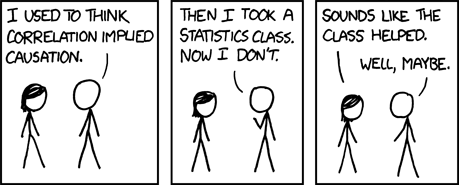
\includegraphics[keepaspectratio,alt={Fonte: xkcd}]{imagens/xkcd-correlation.png}}
\caption{Fonte: xkcd}
\end{figure}

No capítulo anterior, vimos que a ignorabilidade forte nos permite identificar efeitos causais --- mas ela depende de condicionarmos nas covariáveis \emph{certas}. Ficamos com uma pergunta em aberto: como saber quais variáveis incluir em \(\mathbf{X}_i\) para que a ignorabilidade seja plausível? E quais variáveis \emph{não} devemos condicionar?

Neste capítulo, introduzimos uma ferramenta que nos ajuda a responder essas perguntas: os \textbf{grafos acíclicos direcionados} (\emph{Directed Acyclic Graphs}, ou DAGs). Essa abordagem foi desenvolvida na ciência da computação entre os anos 80 e 90 e é associada ao trabalho pioneiro de Pearl (\citeproc{ref-pearl2009}{2009}). Para uma história acessível de como surgiu, ver Pearl and Mackenzie (\citeproc{ref-pearl2018}{2018}).

Abaixo temos um exemplo simples de um DAG:

\pandocbounded{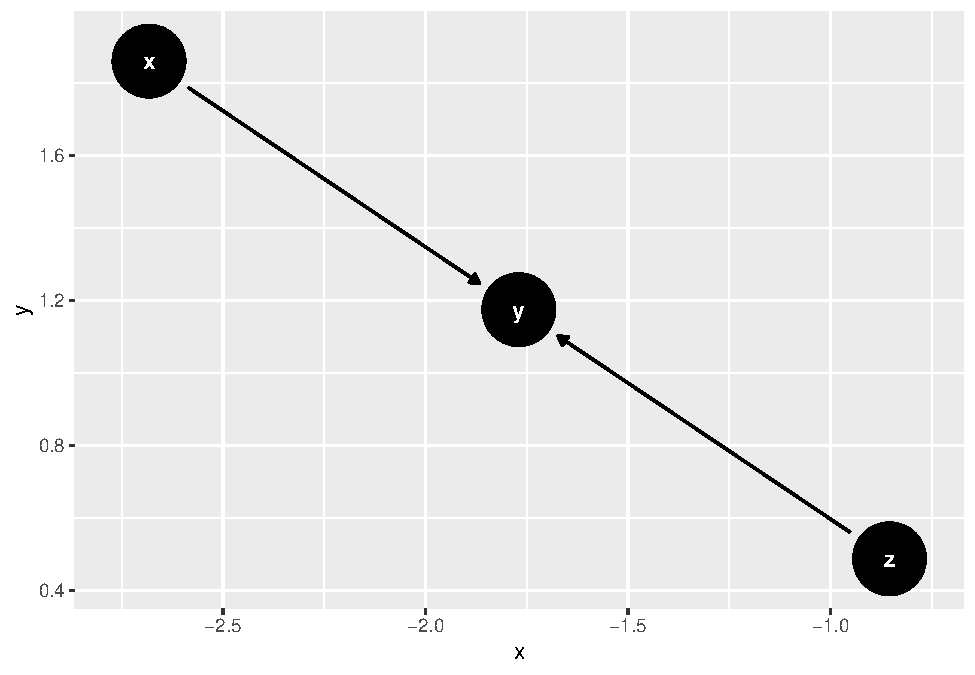
\includegraphics[keepaspectratio]{bookdownproj_files/figure-latex/dag1-1.pdf}}

Eles são chamados de DAGs porque são \textbf{direcionados} (as flechas apontam em uma direção), \textbf{acíclicos} (se \(A\) causa \(B\), então \(B\) não pode causar \(A\)) e \textbf{grafos} (são representações gráficas de relações entre variáveis).

No exemplo acima, o DAG é formado por três variáveis \(\{Y, X, Z\}\), que são, em geral, variáveis aleatórias, e as flechas indicam a direção de causalidade: \(X\) causa \(Y\) e \(Z\) causa \(Y\). É importante saber que DAGs são não paramétricos e podem ser interpretados como \(Y = f(X, Z)\), para qualquer função \(f\). Alguns exemplos compatíveis com o DAG acima:

\begin{itemize}
\tightlist
\item
  \(Y = X + Z\)
\item
  \(Y = 10 + X + Z + X \cdot Z\)
\item
  \(Y = 3 \cdot X^Z\)
\item
  \(Y = \pi \cdot Z/X + X^2 + 1/Z^3\)
\end{itemize}

A razão pela qual não escrevemos DAGs como equações é que \(Y = f(X, Z)\) não expressa adequadamente a relação de causalidade, pois, em matemática, é indiferente escrever \(f(X, Z) = Y\) ou \(Y = f(Z, X)\). Porém, dizer que \(X\) e \(Z\) causam \(Y\) é muito diferente de dizer que \(Y\) causa \(X\) e \(Z\). Com o DAG, as flechas indicam a direção da causalidade.

Na regressão, tentamos capturar essa assimetria com a terminologia: chamamos \(Y\) de ``variável dependente'' ou ``resposta'' e \(X\) de ``variável explicativa'' ou ``independente''. Mas isso é apenas uma convenção de linguagem --- formalmente, nada impede de reescrever a equação isolando \(X\). Por exemplo, se \(Y = \alpha + \beta X + \epsilon\), podemos perfeitamente escrever \(X = (Y - \alpha - \epsilon)/\beta\), e a matemática é igualmente válida. A equação não sabe qual variável é a causa e qual é o efeito. O DAG, por contraste, incorpora a direção causal na própria estrutura: a flecha \(X \to Y\) não pode ser invertida.

\subsection{Os Tipos Básicos de DAGs}\label{os-tipos-buxe1sicos-de-dags}

Qualquer DAG, por mais complexo que seja, é composto por combinações de três estruturas elementares. Compreender como cada uma delas afeta a dependência entre variáveis é a chave para decidir quais variáveis controlar em uma análise causal.

\subsubsection{1. Chain (cadeia)}\label{chain-cadeia}

Em uma \emph{chain}, \(X\) causa \(W\) que, por sua vez, causa \(Y\). Aqui, \(W\) é o \textbf{mediador} do efeito de \(X\) sobre \(Y\).

\textbf{Exemplo:} O desempenho econômico de um país pode aumentar a popularidade do presidente, o que leva a mais votos.

\pandocbounded{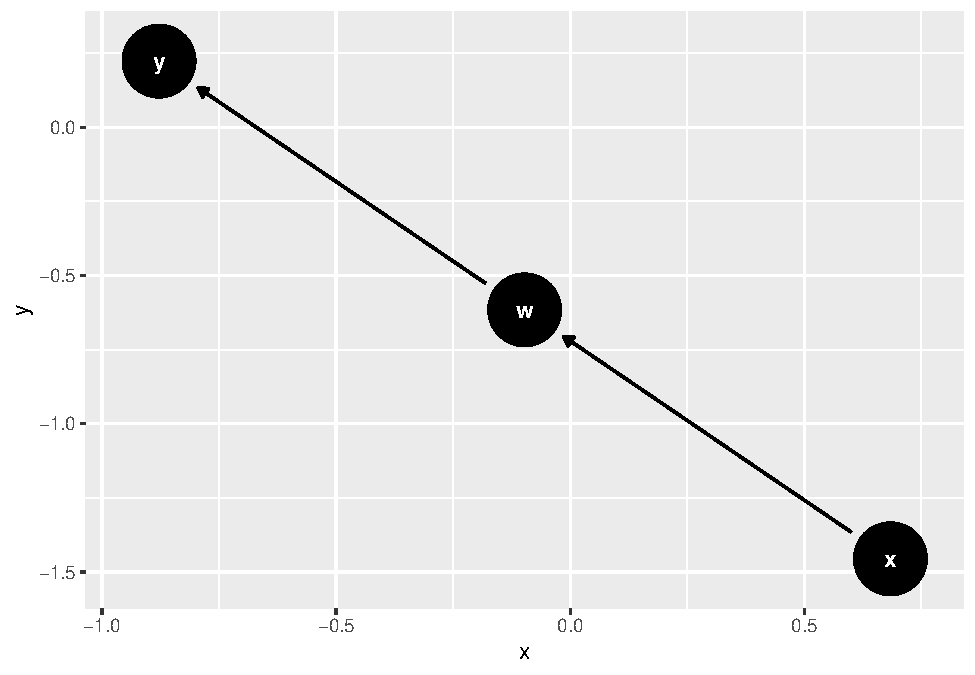
\includegraphics[keepaspectratio]{bookdownproj_files/figure-latex/chain-1.pdf}}

\subsubsection{2. Fork (garfo)}\label{fork-garfo}

Em um \emph{fork}, uma variável \(W\) causa tanto \(X\) quanto \(Y\). Dessa forma, \(W\) é uma \textbf{causa comum} que pode gerar correlação espúria entre \(X\) e \(Y\).

\textbf{Exemplo:} A qualidade de um candidato pode fazer com que ele arrecade mais dinheiro para a campanha e, ao mesmo tempo, obtenha mais votos.

\pandocbounded{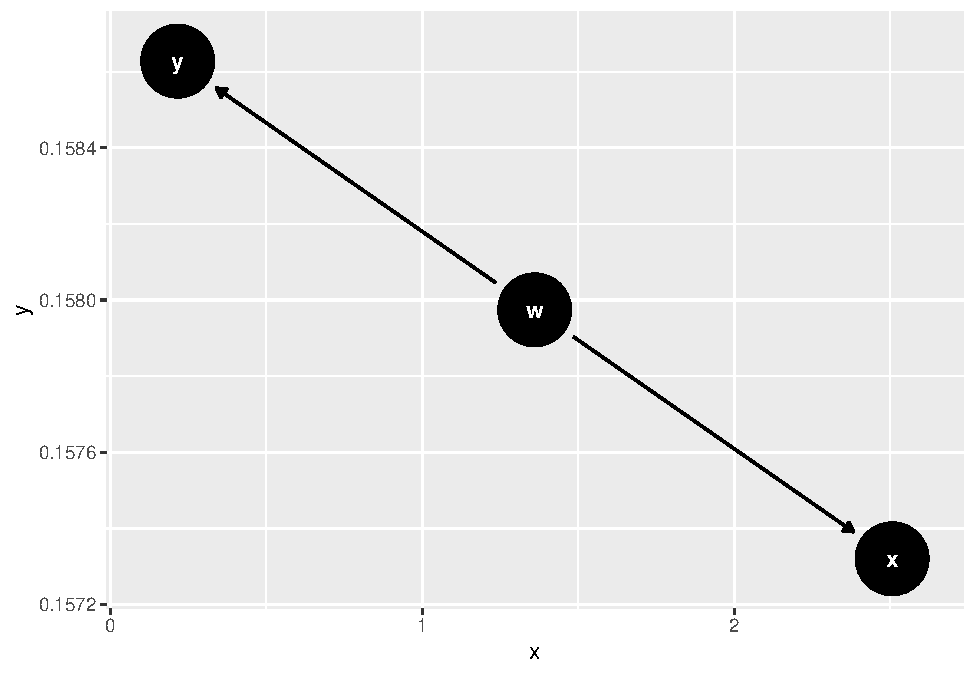
\includegraphics[keepaspectratio]{bookdownproj_files/figure-latex/fork-1.pdf}}

\subsubsection{3. Collider (colisor)}\label{collider-colisor}

Em um \emph{collider}, \(X\) causa \(W\) e \(Y\) também causa \(W\). Esse tipo de estrutura é também chamado de ``fork invertido''. Apesar de \(X\) e \(Y\) não terem relação causal direta, \textbf{controlar para \(W\)} (ou um de seus descendentes) pode introduzir uma correlação espúria entre \(X\) e \(Y\).

\pandocbounded{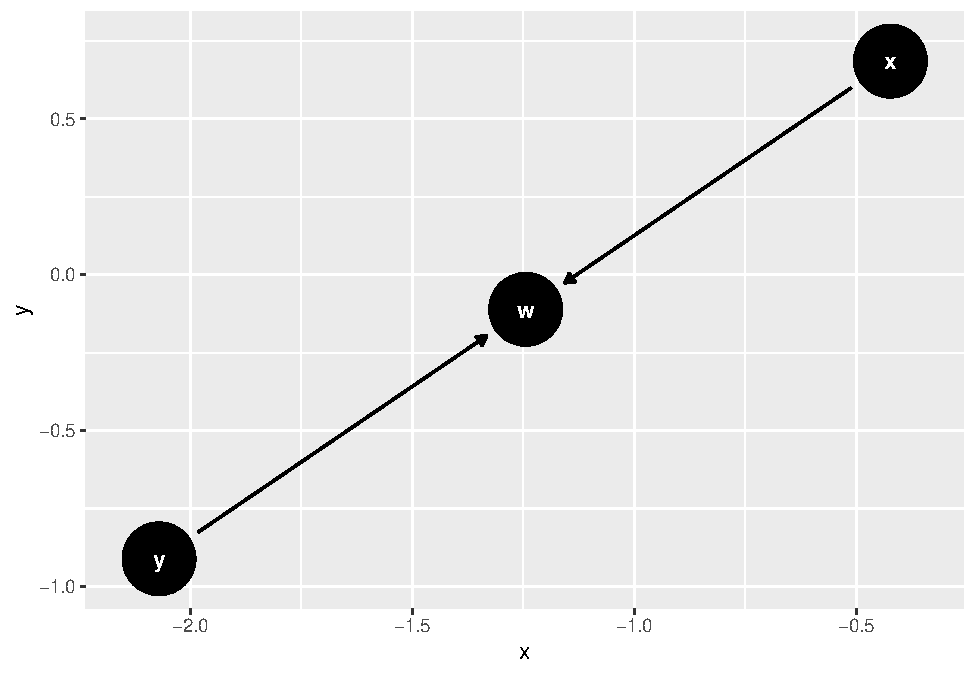
\includegraphics[keepaspectratio]{bookdownproj_files/figure-latex/collider-1.pdf}}

\textbf{Exemplo:} Imagine que você organiza uma festa e convida apenas pessoas que fazem ciência política ou são canhotas. Na população geral, pode não haver relação entre essas características, mas na festa pode surgir uma correlação: se sabemos que uma pessoa está na festa e ela é canhota, é mais provável que ela \emph{não} faça ciência política --- pois a condição de canhota já explica sua presença na festa.

\pandocbounded{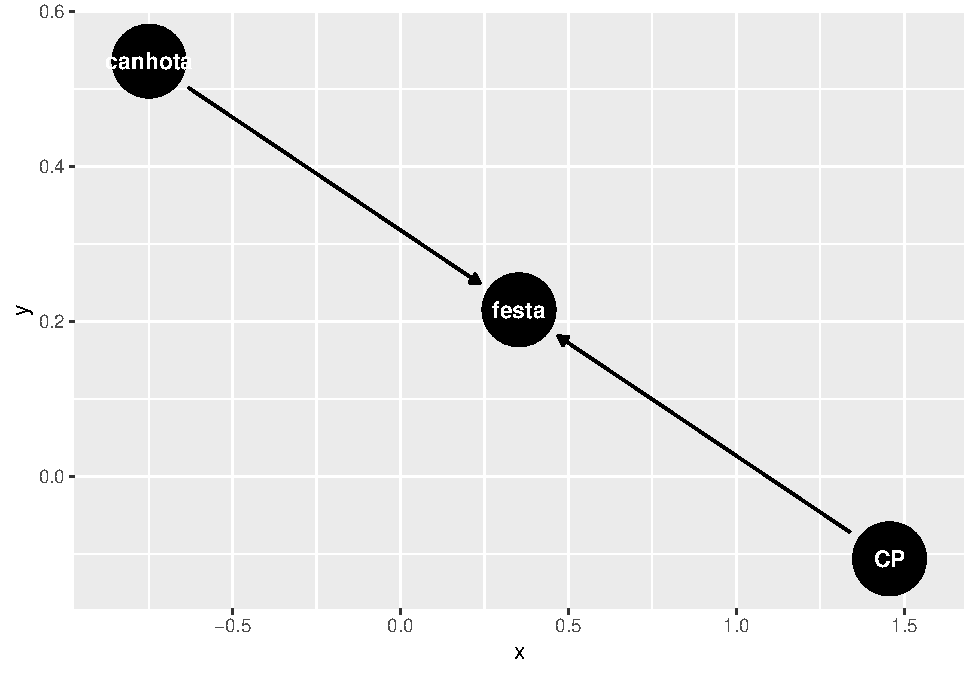
\includegraphics[keepaspectratio]{bookdownproj_files/figure-latex/collider1-1.pdf}}

Esses três tipos --- chains, forks e colliders --- são os blocos fundamentais a partir dos quais qualquer DAG pode ser construído. Vejamos agora uma simulação que ilustra o viés que pode surgir quando condicionamos em um collider.

\subsection{Simulação no R: Ilustrando o Collider Bias}\label{simulauxe7uxe3o-no-r-ilustrando-o-collider-bias}

Vamos rodar uma simulação para ilustrar o collider bias. Suponha que 10\% das pessoas fazem ciência política e 5\% são canhotas, e que essas duas características são independentes na população.

\begin{Shaded}
\begin{Highlighting}[]
\FunctionTok{set.seed}\NormalTok{(}\DecValTok{4}\NormalTok{)}

\CommentTok{\# Gerando as variáveis}
\NormalTok{cp }\OtherTok{\textless{}{-}} \FunctionTok{rbinom}\NormalTok{(}\DecValTok{1000}\NormalTok{, }\DecValTok{1}\NormalTok{, }\AttributeTok{p =} \FloatTok{0.1}\NormalTok{)       }\CommentTok{\# 10\% fazem ciência política}
\NormalTok{canhoto }\OtherTok{\textless{}{-}} \FunctionTok{rbinom}\NormalTok{(}\DecValTok{1000}\NormalTok{, }\DecValTok{1}\NormalTok{, }\AttributeTok{p =} \FloatTok{0.05}\NormalTok{) }\CommentTok{\# 5\% são canhotos}

\CommentTok{\# Condição da festa: convida se faz CP ou é canhoto}
\NormalTok{festa }\OtherTok{\textless{}{-}} \FunctionTok{ifelse}\NormalTok{(cp }\SpecialCharTok{==} \DecValTok{1} \SpecialCharTok{|}\NormalTok{ canhoto }\SpecialCharTok{==} \DecValTok{1}\NormalTok{, }\DecValTok{1}\NormalTok{, }\DecValTok{0}\NormalTok{)}
\NormalTok{tabela }\OtherTok{\textless{}{-}} \FunctionTok{data.frame}\NormalTok{(cp, canhoto, festa)}

\CommentTok{\# Correlação na população geral}
\FunctionTok{cat}\NormalTok{(}\StringTok{"Correlação na população:"}\NormalTok{, }\FunctionTok{round}\NormalTok{(}\FunctionTok{cor}\NormalTok{(cp, canhoto), }\DecValTok{3}\NormalTok{), }\StringTok{"}\SpecialCharTok{\textbackslash{}n}\StringTok{"}\NormalTok{)}
\end{Highlighting}
\end{Shaded}

\begin{verbatim}
## Correla<U+00E7><U+00E3>o na popula<U+00E7><U+00E3>o: -0.016
\end{verbatim}

\begin{Shaded}
\begin{Highlighting}[]
\CommentTok{\# Correlação entre os que foram à festa (condicionando no collider)}
\NormalTok{cor\_festa }\OtherTok{\textless{}{-}}\NormalTok{ tabela }\SpecialCharTok{\%\textgreater{}\%}
  \FunctionTok{filter}\NormalTok{(festa }\SpecialCharTok{==} \DecValTok{1}\NormalTok{) }\SpecialCharTok{\%\textgreater{}\%}
  \FunctionTok{summarise}\NormalTok{(}\AttributeTok{cor =} \FunctionTok{round}\NormalTok{(}\FunctionTok{cor}\NormalTok{(cp, canhoto), }\DecValTok{3}\NormalTok{))}
\FunctionTok{cat}\NormalTok{(}\StringTok{"Correlação na festa (condicionando no collider):"}\NormalTok{, cor\_festa}\SpecialCharTok{$}\NormalTok{cor, }\StringTok{"}\SpecialCharTok{\textbackslash{}n}\StringTok{"}\NormalTok{)}
\end{Highlighting}
\end{Shaded}

\begin{verbatim}
## Correla<U+00E7><U+00E3>o na festa (condicionando no collider): -0.948
\end{verbatim}

Na população em geral, a correlação é próxima de zero. Porém, entre as pessoas que foram à festa, a correlação pode chegar a \(-0{,}95\), evidenciando como condicionar em um collider pode induzir correlação espúria. Esse resultado reforça a importância de entender a estrutura causal antes de decidir por quais variáveis condicionar.

\subsection{Definições Formais}\label{definiuxe7uxf5es-formais}

Agora que temos a intuição dos três tipos básicos, vamos formalizar os conceitos que precisaremos para raciocinar sobre DAGs mais complexos (para uma referência concisa, ver \citeproc{ref-greenland2014}{Greenland and Pearl 2014}).

\subsubsection{Caminhos e relações entre nós}\label{caminhos-e-relauxe7uxf5es-entre-nuxf3s}

\textbf{Caminho} (\emph{path}): uma sequência de nós conectados por flechas, independentemente da direção. Por exemplo, no DAG \(X \to W \leftarrow Y\), existe um caminho entre \(X\) e \(Y\) passando por \(W\).

\textbf{Caminho direcionado} (\emph{directed path}): um caminho em que todas as flechas seguem a mesma direção. Por exemplo, \(X \to W \to Y\) é um caminho direcionado de \(X\) a \(Y\).

\textbf{Relações entre nós} (terminologia da genética):

\begin{itemize}
\tightlist
\item
  \textbf{Pais} de \(Y\): nós com flechas diretas para \(Y\)
\item
  \textbf{Filhos} de \(Y\): nós para os quais \(Y\) tem flechas diretas
\item
  \textbf{Ancestrais} de \(Y\): todos os nós dos quais existe um caminho direcionado até \(Y\)
\item
  \textbf{Descendentes} de \(Y\): todos os nós para os quais existe um caminho direcionado a partir de \(Y\)
\end{itemize}

\subsubsection{d-separação}\label{d-separauxe7uxe3o}

A \textbf{d-separação} (\emph{d} de \emph{directed}) é o conceito central que conecta a estrutura de um DAG às independências estatísticas entre variáveis. Dizemos que dois nós \(X\) e \(Y\) estão \textbf{d-separados} por um conjunto de nós \(\mathbf{Z}\) se todo caminho entre \(X\) e \(Y\) está \textbf{bloqueado} condicional a \(\mathbf{Z}\).

Quando um caminho está bloqueado? Antes de ver as regras, um alerta importante: para determinar se há dependência entre \(X\) e \(Y\), o que importa são \textbf{caminhos} (\emph{paths}), não caminhos direcionados. A direção das flechas determina o \emph{tipo} de cada nó no caminho (fork, chain ou collider), mas a dependência estatística pode fluir em qualquer direção. Uma analogia útil: pense em cada caminho como um cano com água. Se o cano está aberto, a água pode fluir em qualquer direção --- não apenas na direção das flechas. Estudantes frequentemente cometem o erro de achar que a dependência só ``viaja'' na direção das flechas; na verdade, um fork \(X \leftarrow W \to Y\) transmite dependência de \(X\) a \(Y\) mesmo que nenhuma flecha aponte de \(X\) para \(Y\).

As regras de bloqueio derivam diretamente dos três tipos básicos:

\begin{enumerate}
\def\labelenumi{\arabic{enumi}.}
\item
  \textbf{Chain} (\(X \to W \to Y\)): o caminho está \textbf{aberto} por padrão. Condicionar em \(W\) \textbf{bloqueia} o caminho.
\item
  \textbf{Fork} (\(X \leftarrow W \to Y\)): o caminho está \textbf{aberto} por padrão (a causa comum \(W\) transmite dependência). Condicionar em \(W\) \textbf{bloqueia} o caminho.
\item
  \textbf{Collider} (\(X \to W \leftarrow Y\)): o caminho está \textbf{fechado} por padrão. Condicionar em \(W\) (ou em qualquer descendente de \(W\)) \textbf{abre} o caminho.
\end{enumerate}

A regra geral: um caminho está bloqueado se contém pelo menos um nó que (a) é um não-collider (chain ou fork) e está no conjunto \(\mathbf{Z}\), ou (b) é um collider e nem ele nem seus descendentes estão em \(\mathbf{Z}\).

\textbf{Exemplo trabalhado.} Considere o seguinte DAG:

\pandocbounded{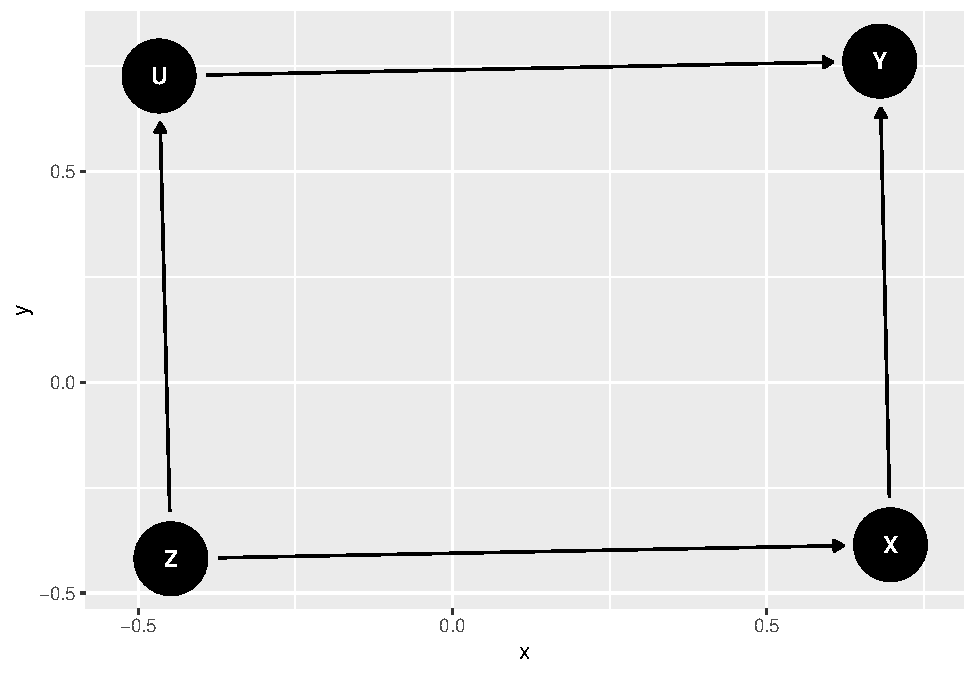
\includegraphics[keepaspectratio]{bookdownproj_files/figure-latex/dsep-example-1.pdf}}

Quais caminhos existem entre \(X\) e \(Y\)?

\begin{enumerate}
\def\labelenumi{\arabic{enumi}.}
\tightlist
\item
  \(X \to Y\) --- caminho direcionado (causal), sempre aberto
\item
  \(X \leftarrow Z \to U \to Y\) --- caminho com estrutura de fork centrada em \(Z\)
\end{enumerate}

O caminho 2 é um \textbf{backdoor path}: ele conecta \(X\) a \(Y\) por trás, transmitindo dependência espúria via \(Z\). Para bloquear esse caminho, podemos condicionar em \(Z\) (que é a causa comum no centro do fork \(X \leftarrow Z \to U\)). Nesse caso, \(X\) e \(Y\) ficam d-separados de toda influência espúria, e a associação remanescente reflete apenas o efeito causal de \(X\) sobre \(Y\).

\emph{Pare e pense:} e se condicionássemos em \(U\) em vez de \(Z\)? O caminho 2 seria bloqueado? (Resposta: sim, pois \(U\) é um não-collider nesse caminho, e condicionar nele bloqueia a transmissão.)

\subsection{Controle e Ajuste}\label{controle-e-ajuste}

Agora que entendemos d-separação, podemos abordar a questão central: como decidir quais variáveis controlar em uma análise causal?

\subsubsection{Condicionar vs.~intervir}\label{condicionar-vs.-intervir}

No contexto dos DAGs, ``controlar'' pode significar duas coisas diferentes:

\begin{enumerate}
\def\labelenumi{\arabic{enumi}.}
\item
  \textbf{Intervir} (experimento): determinamos exogenamente o valor da variável. No DAG, isso equivale a \textbf{remover todas as flechas que entram} no nó manipulado --- pois o valor da variável não é mais determinado por suas causas, mas pelo pesquisador.
\item
  \textbf{Condicionar} (estudo observacional): estratificamos, incluímos como controle numa regressão, ou restringimos a amostra a um subgrupo. No DAG, isso \textbf{bloqueia caminhos} que passam pelo nó condicionado (se for fork/chain) ou \textbf{abre caminhos} (se for collider).
\end{enumerate}

\subsubsection{O que acontece ao condicionar}\label{o-que-acontece-ao-condicionar}

Vamos ilustrar com um DAG concreto. Suponha que queremos estimar o efeito de \(X\) sobre \(Y\):

\pandocbounded{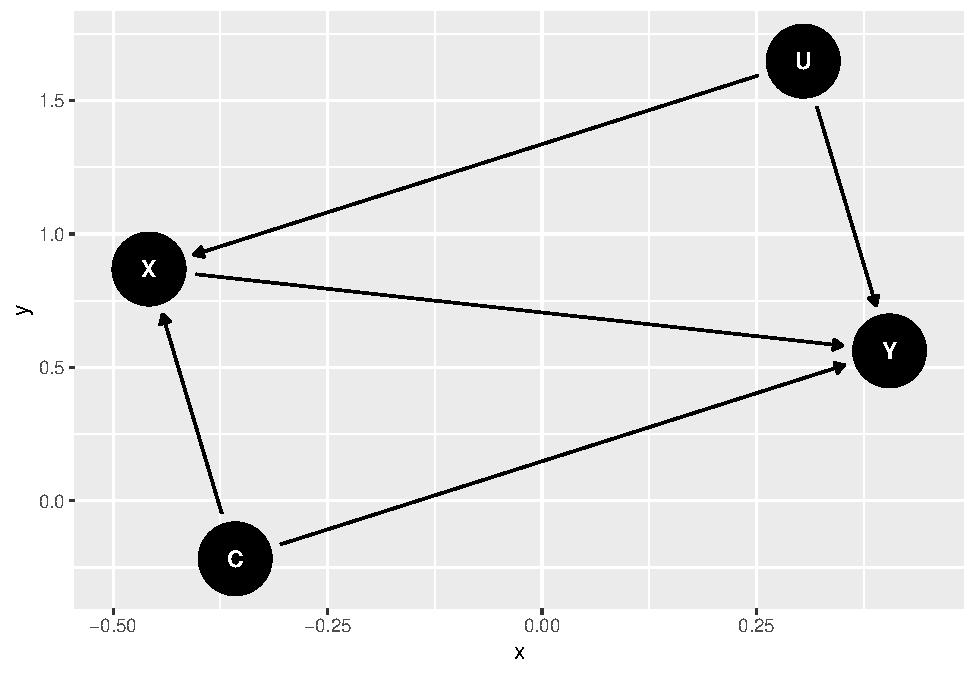
\includegraphics[keepaspectratio]{bookdownproj_files/figure-latex/ajuste-exemplo-1.pdf}}

Caminhos entre \(X\) e \(Y\):

\begin{enumerate}
\def\labelenumi{\arabic{enumi}.}
\tightlist
\item
  \(X \to Y\) --- causal (aberto, queremos preservar)
\item
  \(X \leftarrow C \to Y\) --- backdoor via fork com causa comum \(C\) (aberto, causa viés)
\item
  \(X \leftarrow U \to Y\) --- backdoor via fork com causa comum \(U\) (aberto, causa viés)
\end{enumerate}

Se condicionarmos em \(C\), bloqueamos o caminho 2. Se \(U\) for não observável, não conseguimos condicionar nele e o caminho 3 permanece aberto --- nesse caso, nosso estimador ainda será viesado. Isso ilustra um ponto importante: \textbf{condicionar em algumas variáveis pode reduzir o viés sem eliminá-lo completamente}.

E se condicionássemos em \(U\) também? Nesse caso, todos os backdoor paths estariam bloqueados, e a associação entre \(X\) e \(Y\) refletiria apenas o efeito causal. O conjunto \(\{C, U\}\) satisfaz o \textbf{critério backdoor}, que formalizamos a seguir.

\subsubsection{O que dá errado ao condicionar em um collider}\label{o-que-duxe1-errado-ao-condicionar-em-um-collider}

Nem sempre mais controles são melhores. Considere uma pesquisadora que estuda o efeito da educação (\(E\)) sobre a renda (\(R\)). Ela observa que habilidade inata (\(H\)) também afeta a renda, e que tanto educação quanto habilidade determinam se a pessoa é aprovada em um concurso público (\(A\)):

\pandocbounded{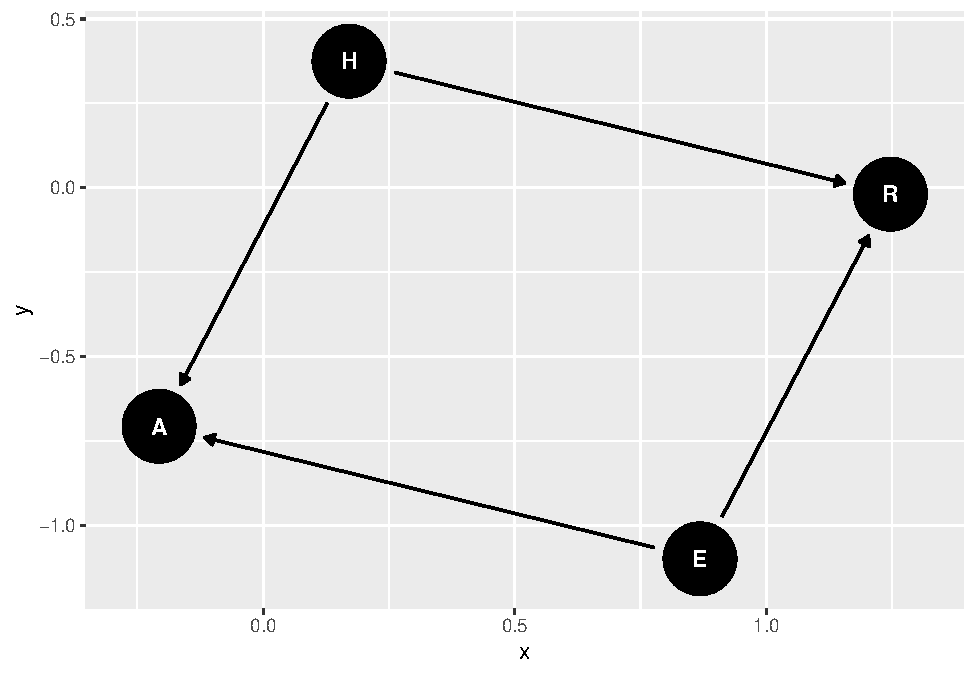
\includegraphics[keepaspectratio]{bookdownproj_files/figure-latex/collider-erro-1.pdf}}

Caminhos entre \(E\) e \(R\):

\begin{enumerate}
\def\labelenumi{\arabic{enumi}.}
\tightlist
\item
  \(E \to R\) --- causal (aberto)
\item
  \(E \to A \leftarrow H \to R\) --- collider em \(A\) (\textbf{fechado} por padrão)
\end{enumerate}

Sem condicionar em nada, a associação entre \(E\) e \(R\) reflete apenas o efeito causal --- o caminho 2 já está bloqueado pelo collider. Porém, se a pesquisadora incluir \(A\) (aprovação no concurso) como controle na regressão --- ``para aumentar a precisão'' --- ela \textbf{abre} o caminho 2 e cria uma associação espúria entre \(E\) e \(H\) dentro de cada nível de \(A\). O resultado é um estimador \emph{mais} viesado do que a regressão simples sem controles.

A lição: \textbf{controlar por variáveis pós-tratamento ou por colliders pode introduzir viés onde não havia}. O critério backdoor formaliza quando é seguro condicionar.

\subsection{O Critério Backdoor}\label{o-crituxe9rio-backdoor}

O critério backdoor, formulado por Pearl (\citeproc{ref-pearl2009}{2009}), é a ferramenta que nos permite determinar sistematicamente quais variáveis controlar para identificar um efeito causal. Ele responde diretamente à pergunta que deixamos em aberto no Cap. 2: quais covariáveis \(\mathbf{X}_i\) tornam a ignorabilidade plausível?

\textbf{Definição.} Um conjunto de variáveis \(\mathbf{Z}\) satisfaz o \textbf{critério backdoor} em relação ao par ordenado \((X, Y)\) se:

\begin{enumerate}
\def\labelenumi{\arabic{enumi}.}
\tightlist
\item
  Nenhum nó em \(\mathbf{Z}\) é descendente de \(X\)
\item
  \(\mathbf{Z}\) bloqueia todo caminho entre \(X\) e \(Y\) que contém uma flecha entrando em \(X\) (todo \emph{backdoor path})
\end{enumerate}

Se \(\mathbf{Z}\) satisfaz o critério backdoor, então o efeito causal de \(X\) sobre \(Y\) é identificado pela \textbf{fórmula de ajuste}: basta comparar tratados e controles \emph{dentro de cada estrato} de \(\mathbf{Z}\) e depois agregar:

\[\text{Efeito causal} = \sum_{z} \left[P(Y = y \mid X = x, \mathbf{Z} = z) - P(Y = y \mid X = x', \mathbf{Z} = z)\right] P(\mathbf{Z} = z)\]

Em palavras: condicionamos em \(\mathbf{Z}\) para bloquear todos os backdoor paths, calculamos a diferença entre tratados e controles em cada estrato, e ponderamos pela distribuição marginal de \(\mathbf{Z}\). Na seção 3.8, veremos como essa fórmula se conecta ao operador \(do()\) de Pearl.

\textbf{Conexão com resultados potenciais.} O critério backdoor é a contrapartida gráfica da ignorabilidade condicional do Cap. 2. Se \(\mathbf{Z}\) satisfaz o critério backdoor, então \(Y(1), Y(0) \perp D \mid \mathbf{Z}\) --- exatamente a condição 1 da ignorabilidade forte. Compare com o Teorema 1 do Cap. 2: a fórmula de ajuste acima tem a mesma estrutura. A condição 2 (common support) precisa ser verificada nos dados.

\textbf{Exemplo.} Considere o seguinte DAG sobre o efeito do gasto de campanha (\(X\)) sobre os votos (\(Y\)):

\pandocbounded{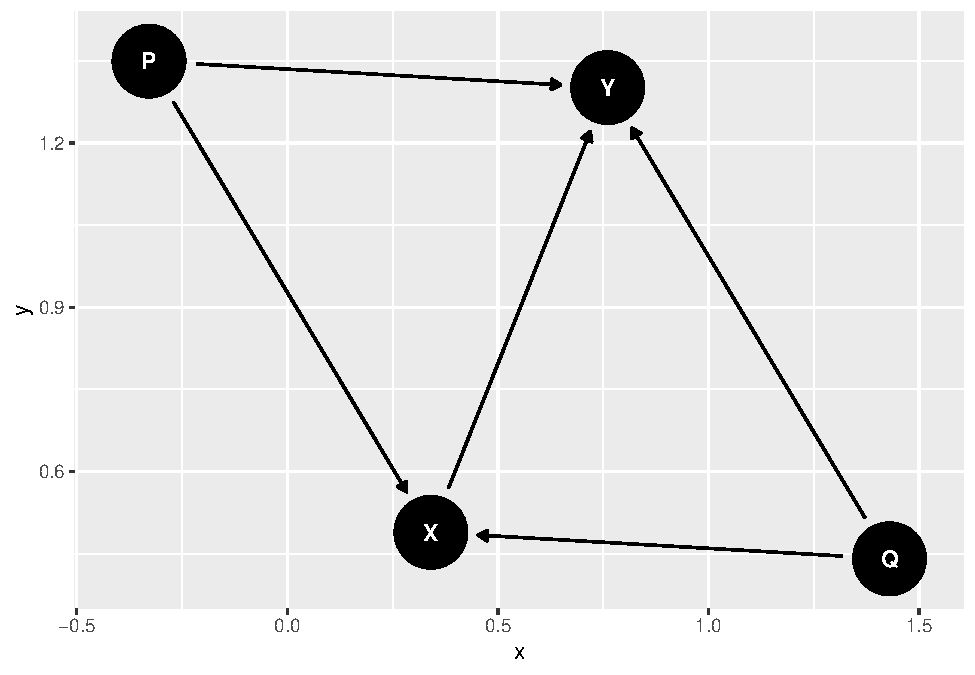
\includegraphics[keepaspectratio]{bookdownproj_files/figure-latex/backdoor-exemplo-1.pdf}}

Onde \(Q\) = qualidade do candidato e \(P\) = partido. Caminhos entre \(X\) e \(Y\):

\begin{enumerate}
\def\labelenumi{\arabic{enumi}.}
\tightlist
\item
  \(X \to Y\) --- causal
\item
  \(X \leftarrow Q \to Y\) --- backdoor (fork com causa comum \(Q\))
\item
  \(X \leftarrow P \to Y\) --- backdoor (fork com causa comum \(P\))
\end{enumerate}

O único conjunto mínimo que satisfaz o critério backdoor é \(\{Q, P\}\). Controlar apenas por \(\{Q\}\) não basta (caminho 3 permanece aberto) e apenas por \(\{P\}\) também não (caminho 2 permanece aberto). Logo, precisamos controlar por ambos.

\emph{Pare e pense:} e se houvesse uma variável \(M\) (mídia) tal que \(X \to M \to Y\)? Poderíamos incluir \(M\) no conjunto de ajuste? (Resposta: não --- \(M\) é descendente de \(X\), violando a condição 1. Controlar por \(M\) bloquearia parte do efeito causal que queremos estimar.)

\subsection{\texorpdfstring{O Operador \emph{do}}{O Operador do}}\label{o-operador-do}

Até aqui, falamos em ``condicionar'' e ``intervir'' informalmente. O operador \(do()\), introduzido por Pearl (\citeproc{ref-pearl2009}{2009}), formaliza a diferença.

\subsubsection{Observar vs.~intervir}\label{observar-vs.-intervir}

\begin{itemize}
\item
  \(P(Y \mid X = x)\) é a probabilidade de \(Y\) dado que \textbf{observamos} \(X = x\). Ela reflete tanto o efeito causal de \(X\) sobre \(Y\) quanto qualquer associação espúria via caminhos backdoor.
\item
  \(P(Y \mid do(X = x))\) é a probabilidade de \(Y\) quando \textbf{intervenimos} fixando \(X = x\). No DAG, isso corresponde a uma ``cirurgia'': removemos todas as flechas que entram em \(X\) (pois o valor de \(X\) agora é determinado pela intervenção, não por suas causas) e calculamos a distribuição de \(Y\) no DAG modificado.
\end{itemize}

\subsubsection{Quando observar = intervir?}\label{quando-observar-intervir}

Se não há confounding --- ou seja, não há backdoor path aberto entre \(X\) e \(Y\) --- então a distribuição observacional é igual à distribuição intervencional:

\pandocbounded{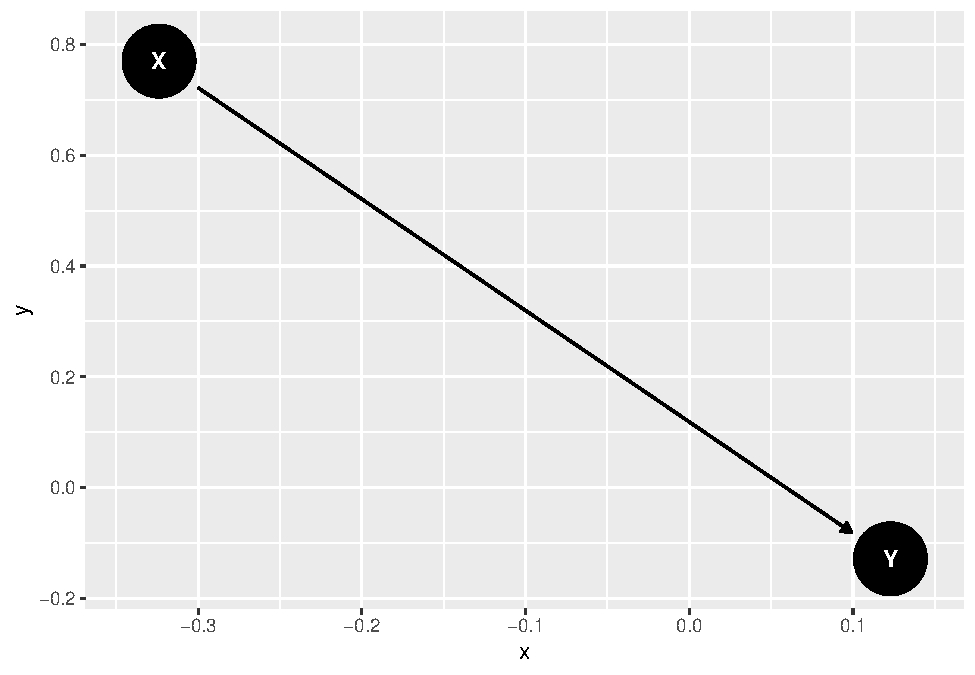
\includegraphics[keepaspectratio]{bookdownproj_files/figure-latex/do-sem-confounding-1.pdf}}

\[P(Y \mid do(X = x)) = P(Y \mid X = x)\]

Porém, quando há confounding, as duas diferem:

\pandocbounded{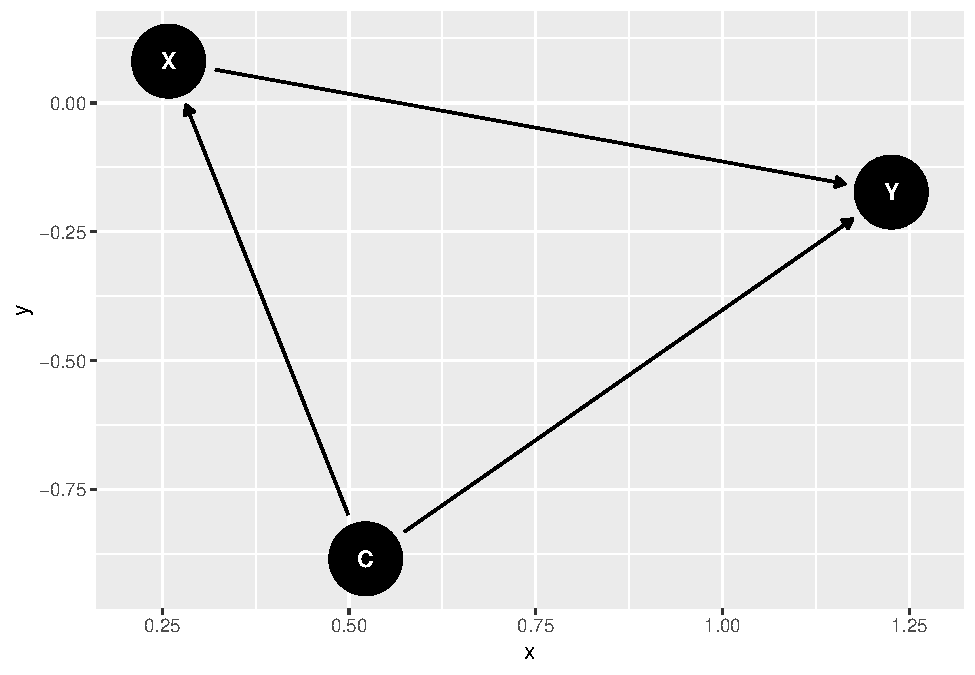
\includegraphics[keepaspectratio]{bookdownproj_files/figure-latex/do-com-confounding-1.pdf}}

Aqui, \(P(Y \mid X = x) \neq P(Y \mid do(X = x))\), porque observar \(X = x\) traz informação sobre \(C\) (via o caminho \(X \leftarrow C\)), que por sua vez afeta \(Y\). Já ao intervir com \(do(X = x)\), cortamos essa conexão.

O critério backdoor nos diz exatamente como calcular \(P(Y \mid do(X = x))\) a partir de dados observacionais. Com a notação \(do()\), a fórmula de ajuste da seção anterior pode ser reescrita como:

\[P(Y = y \mid do(X = x)) = \sum_{z} P(Y = y \mid X = x, \mathbf{Z} = z) \, P(\mathbf{Z} = z)\]

O lado esquerdo é a quantidade causal que queremos; o lado direito contém apenas quantidades observacionais --- condicionamentos e probabilidades marginais que podemos estimar com dados.

\begin{quote}
\textbf{Nota técnica: fatorização da probabilidade conjunta.} Esta seção é mais formal e pode ser pulada em uma primeira leitura. Ela conecta a estrutura de um DAG à distribuição de probabilidade conjunta das variáveis, explicando \emph{por que} d-separação implica independência estatística.

Toda distribuição de probabilidade obedece à \textbf{regra da cadeia}: \(P(X_1, \ldots, X_k) = P(X_1) \, P(X_2 \mid X_1) \cdots P(X_k \mid X_1, \ldots, X_{k-1})\). Para \(n\) variáveis, existem \(n!\) fatorizações possíveis. Porém, um DAG impõe restrições: cada nó é condicionalmente independente de seus não-descendentes, dados seus pais. Isso gera a \textbf{fatorização Markoviana}:

\[P(X_1, \ldots, X_k) = \prod_{i=1}^{k} P(X_i \mid \text{Pais}(X_i))\]

Cada fator condiciona apenas nos pais diretos --- muito mais parcimonioso que a regra da cadeia genérica. O exemplo abaixo ilustra.

\textbf{Conexão com causalidade.} Quando não há confounding (sem backdoor path aberto), a fatorização observacional coincide com a intervencional: \(P(Y, X) = P(X) \, P(Y \mid X) = P(X) \, P(Y \mid do(X))\). Essa igualdade é o que torna a inferência causal possível a partir de dados observacionais quando o critério backdoor é satisfeito.
\end{quote}

\textbf{Exemplo de fatorização Markoviana.} Considere o DAG:

\pandocbounded{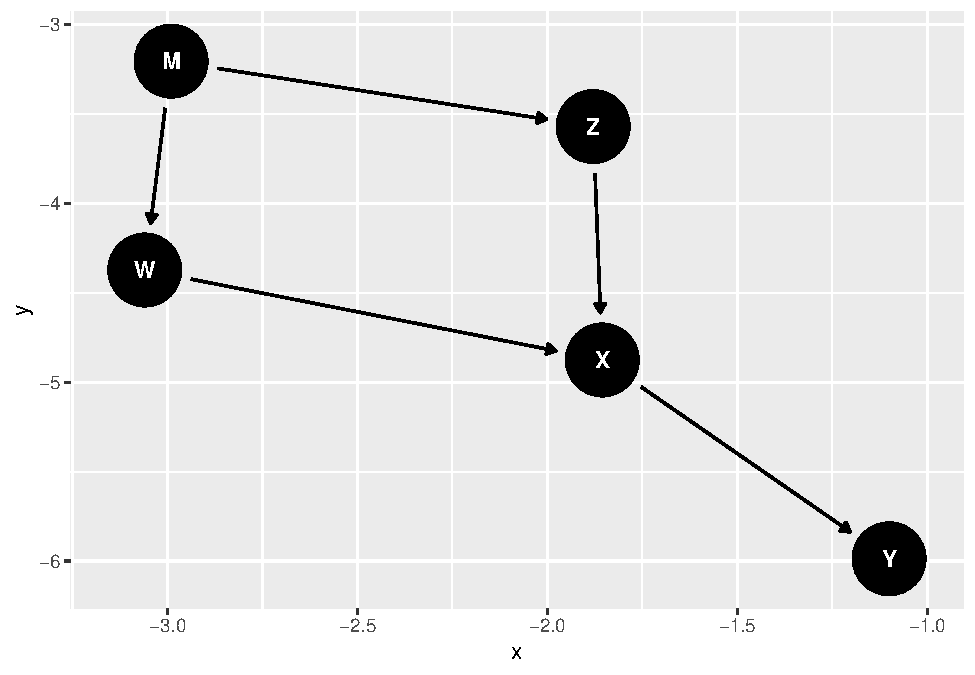
\includegraphics[keepaspectratio]{bookdownproj_files/figure-latex/fatorizacao-1.pdf}}

Os pais de cada nó são: \(M\) não tem pais; \(Z\) e \(W\) têm pai \(M\); \(X\) tem pais \(Z\) e \(W\); \(Y\) tem pai \(X\). Logo, a fatorização Markoviana é:

\[P(M, Z, W, X, Y) = P(M) \, P(Z \mid M) \, P(W \mid M) \, P(X \mid W, Z) \, P(Y \mid X)\]

\subsection{Limitações dos DAGs}\label{limitauxe7uxf5es-dos-dags}

DAGs são uma ferramenta poderosa, mas não são uma solução universal. É importante ter em mente suas limitações:

\begin{enumerate}
\def\labelenumi{\arabic{enumi}.}
\item
  \textbf{O DAG precisa estar correto.} Toda a análise depende de o pesquisador especificar corretamente a estrutura causal. Se uma flecha estiver faltando (variável confundidora omitida) ou apontando na direção errada, as conclusões sobre o que controlar podem ser equivocadas. O DAG não é testável --- ele codifica suposições.
\item
  \textbf{Não capturam ciclos de feedback.} DAGs são, por definição, acíclicos. Relações de feedback simultâneo (ex: democracia afeta crescimento, que afeta democracia) não podem ser representadas diretamente. Para esses casos, existem extensões como grafos direcionados cíclicos e modelos de equações estruturais simultâneas, mas estão fora do escopo deste curso.
\item
  \textbf{Não dizem \emph{quanto}.} DAGs são qualitativos: indicam \emph{se} um efeito causal é identificável e \emph{quais} variáveis controlar, mas não dizem nada sobre a magnitude do efeito ou a forma funcional da relação. Para isso, precisamos combinar o DAG com um método de estimação (regressão, matching, etc.).
\end{enumerate}

\subsection{Resumo e próximos passos}\label{resumo-e-pruxf3ximos-passos-2}

Neste capítulo, introduzimos os DAGs como ferramenta para representar e raciocinar sobre relações causais:

\begin{enumerate}
\def\labelenumi{\arabic{enumi}.}
\item
  \textbf{Três tipos básicos.} Chains, forks e colliders determinam quais caminhos estão abertos ou fechados. Condicionar fecha caminhos via forks/chains, mas abre caminhos via colliders.
\item
  \textbf{d-separação.} Dois nós estão d-separados se todo caminho entre eles está bloqueado. As regras de bloqueio derivam diretamente dos três tipos básicos.
\item
  \textbf{Critério backdoor.} Um conjunto \(\mathbf{Z}\) identifica o efeito causal se bloqueia todos os backdoor paths sem incluir descendentes do tratamento. Esse critério é a contrapartida gráfica da ignorabilidade condicional do Cap. 2.
\item
  \textbf{Operador \(do()\).} Distingue a distribuição observacional \(P(Y \mid X)\) da intervencional \(P(Y \mid do(X))\). A fórmula de ajuste backdoor conecta as duas.
\end{enumerate}

No próximo capítulo, veremos por que \textbf{experimentos aleatórios} são considerados o padrão-ouro para inferência causal: a aleatorização garante, por construção, que não haja backdoor paths abertos entre o tratamento e o resultado.

\subsection{Exercícios}\label{exercuxedcios}

\textbf{Exercício 1.} Considere o seguinte DAG:

\pandocbounded{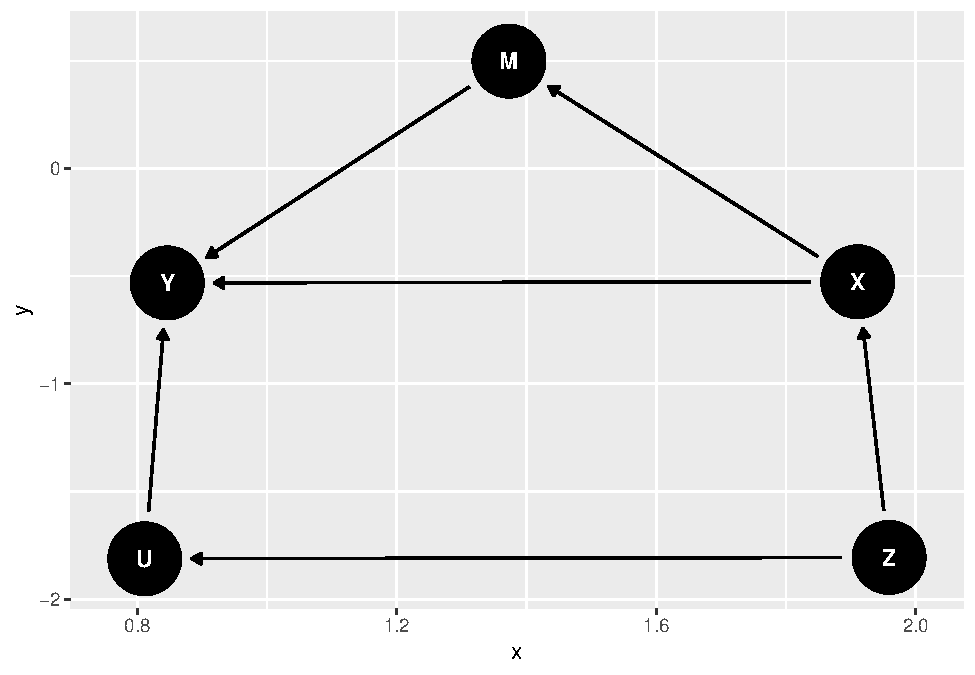
\includegraphics[keepaspectratio]{bookdownproj_files/figure-latex/ex1-1.pdf}}

\begin{enumerate}
\def\labelenumi{(\alph{enumi})}
\item
  Liste todos os caminhos entre \(X\) e \(Y\).
\item
  Classifique cada caminho como causal (direcionado) ou backdoor.
\item
  Quais caminhos estão abertos e quais estão fechados (sem condicionar em nada)?
\item
  Encontre um conjunto de variáveis que satisfaz o critério backdoor.
\end{enumerate}

\textbf{Exercício 2.} Uma pesquisadora quer estimar o efeito da democracia (\(D\)) sobre o crescimento econômico (\(G\)). Ela acredita que: (i) a riqueza inicial (\(W\)) afeta tanto a probabilidade de democratização quanto o crescimento futuro; (ii) a educação (\(E\)) é causada pela riqueza e afeta tanto a democracia quanto o crescimento; (iii) a democracia afeta o crescimento.

\begin{enumerate}
\def\labelenumi{(\alph{enumi})}
\item
  Desenhe o DAG correspondente.
\item
  Identifique os backdoor paths entre \(D\) e \(G\).
\item
  Qual é o conjunto mínimo de variáveis para satisfazer o critério backdoor? A pesquisadora deveria controlar por educação?
\end{enumerate}

\textbf{Exercício 3.} Um cientista político estuda o efeito de ser incumbente (\(I\)) sobre o voto (\(V\)). Ele inclui como controle a cobertura da mídia (\(M\)), argumentando que ``quanto mais controles, melhor''. Porém, ele acredita que ser incumbente causa mais cobertura da mídia, e que a cobertura da mídia causa mais votos (\(I \to M \to V\)).

\begin{enumerate}
\def\labelenumi{(\alph{enumi})}
\item
  Desenhe o DAG e identifique o que \(M\) é nessa estrutura (mediador, confundidor ou collider).
\item
  Explique por que controlar por \(M\) é problemático.
\item
  Em que situação \emph{seria} correto controlar por \(M\)?
\end{enumerate}

\section{Experimentos}\label{experimentos}

\subsection{Introdução}\label{introduuxe7uxe3o-2}

No Cap. 2, mostramos que a ignorabilidade forte --- independência entre resultados potenciais e tratamento, condicional a \(\mathbf{X}_i\) --- identifica o ATE. No Cap. 3, vimos que o critério backdoor nos diz \emph{quais} covariáveis incluir para garantir essa independência. Agora veremos o caso ideal: quando a pesquisadora \emph{controla} o mecanismo de atribuição do tratamento --- o \textbf{experimento aleatório} --- e a ignorabilidade é garantida por construção.

Um experimento é o desenho de pesquisa no qual a pesquisadora controla o mecanismo de atribuição do tratamento. Seja \(p_i = P(D_i = 1)\) a probabilidade de a unidade \(i\) receber o tratamento. Em um experimento, \(p_i\) é conhecido e controlado pela pesquisadora. Em contraposição, um estudo observacional é quando a pesquisadora não controla esse mecanismo --- ele é determinado pela natureza ou pela realidade social.

Neste capítulo, veremos por que experimentos produzem identificação causal crível. Vamos supor condições ideais: sem \emph{attrition} (perda de participantes) e com \emph{compliance} perfeito (todos recebem o tratamento atribuído). Continuamos supondo SUTVA (Cap. 2): não há interferência entre unidades e o tratamento é definido de forma não ambígua.

\subsection{Recapitulação: SDO e viés de seleção}\label{recapitulauxe7uxe3o-sdo-e-viuxe9s-de-seleuxe7uxe3o}

No Cap. 2, derivamos que a simples diferença de médias (SDO, \emph{Simple Difference in Outcomes}) pode ser decomposta em efeito causal mais viés:

\[\underbrace{\mathbb{E}[Y_i \mid D_i=1] - \mathbb{E}[Y_i \mid D_i=0]}_{\text{SDO}} = \underbrace{\mathbb{E}[Y_i(1) - Y_i(0) \mid D_i=1]}_{\text{ATT}} + \underbrace{\mathbb{E}[Y_i(0) \mid D_i=1] - \mathbb{E}[Y_i(0) \mid D_i=0]}_{\text{Viés de Seleção}}\]

O viés de seleção surge quando tratados e controles diferem sistematicamente nos resultados potenciais de base. A questão central deste capítulo é: \textbf{como a aleatorização elimina esse viés?}

\subsection{Experimentos aleatórios e identificação}\label{experimentos-aleatuxf3rios-e-identificauxe7uxe3o}

Um experimento aleatório satisfaz duas condições:

\begin{enumerate}
\def\labelenumi{\arabic{enumi}.}
\item
  \textbf{Positividade}: toda unidade tem probabilidade positiva de receber tratamento ou controle: \(0 < p_i < 1\).
\item
  \textbf{Permutabilidade} (\emph{unconfoundedness}): os resultados potenciais são independentes do tratamento: \(Y_i(1), Y_i(0) \perp D_i\).
\end{enumerate}

Em termos do Cap. 3, a aleatorização garante que não haja backdoor paths abertos entre o tratamento e o resultado --- pois o tratamento não tem causas que também afetem \(Y\).

O que a permutabilidade implica? Se os resultados potenciais são independentes do tratamento, então:

\[\mathbb{E}[Y_i(0) \mid D_i=1] = \mathbb{E}[Y_i(0) \mid D_i=0] = \mathbb{E}[Y_i(0)]\]

Ou seja, o viés de seleção desaparece:

\[\mathbb{E}[Y_i(0) \mid D_i=1] - \mathbb{E}[Y_i(0) \mid D_i=0] = 0\]

Portanto, sob aleatorização, a SDO estima o ATT. E como a permutabilidade também implica \(\mathbb{E}[Y_i(1) \mid D_i=1] = \mathbb{E}[Y_i(1)]\), o ATT é igual ao ATE:

\[\text{SDO} = \text{ATT} = \tau_{\text{ATE}}\]

\emph{Pare e pense:} se a condição de tratamento fosse hipoteticamente trocada --- todos os tratados passassem para o controle e vice-versa --- os resultados esperados permaneceriam os mesmos? Essa é a intuição da permutabilidade.

\subsection{Restrição de Exclusão}\label{restriuxe7uxe3o-de-exclusuxe3o}

A aleatorização por si só não basta. Precisamos também que o que afeta \(Y\) seja o tratamento \textbf{efetivamente recebido}, e não o mero fato de ter sido \emph{alocado} para o tratamento. Formalmente, podemos separar a alocação do tratamento \(Z_i\) do tratamento efetivamente recebido \(D_i\).

A \textbf{restrição de exclusão} diz que os resultados potenciais dependem apenas de \(D_i\), não de \(Z_i\):

\[Y_i(D_i, Z_i = 1) = Y_i(D_i, Z_i = 0) = Y_i(D_i)\]

Quando essa condição pode ser violada? Quando o mecanismo de alocação dispara outras causas que afetam \(Y\). Dois exemplos:

\begin{enumerate}
\def\labelenumi{\arabic{enumi}.}
\item
  \textbf{Contaminação.} Suponha que um experimento testa o efeito de transferência de renda sobre bem-estar. Se ONGs, sabendo do experimento, ajudarem quem não recebeu o tratamento, a alocação \(Z_i\) afeta \(Y_i\) por um canal diferente do tratamento.
\item
  \textbf{Erro de mensuração assimétrico.} Se pesquisadores distintos entrevistam tratados e controles, ou se questionários diferentes são usados para cada grupo, o erro de mensuração pode diferir sistematicamente. Seja \(e_{i,1}\) o erro de mensuração para tratados e \(e_{i,0}\) para controles. A switching equation se torna:
\end{enumerate}

\[Y_i^{obs} = D_i \cdot (Y_i(1) + e_{i,1}) + (1 - D_i) \cdot (Y_i(0) + e_{i,0})\]

Nesse caso, a SDO inclui um termo adicional \(\mathbb{E}[e_{i,1} \mid D_i=1] - \mathbb{E}[e_{i,0} \mid D_i=0]\), que introduz viés mesmo com aleatorização perfeita.

\textbf{Como garantir a restrição de exclusão?}

\begin{itemize}
\tightlist
\item
  \textbf{Duplo cego} (\emph{double blindness}): nem o participante nem o pesquisador sabem quem recebeu o tratamento.
\item
  \textbf{Paralelismo na administração}: mesmo questionário, mesmos entrevistadores, mesmo protocolo para ambos os grupos.
\item
  Na pior das hipóteses, \textbf{aleatorização dos entrevistadores} entre os grupos.
\end{itemize}

\subsection{Tipos de aleatorização}\label{tipos-de-aleatorizauxe7uxe3o}

\subsubsection{Aleatorização de Bernoulli}\label{aleatorizauxe7uxe3o-de-bernoulli}

É a aleatorização mais simples: para cada unidade, jogamos uma moeda com probabilidade \(p\) de tratamento. Matematicamente, \(P(D_i = 1) = p\) independentemente para cada \(i\).

O problema é que o número de tratados é aleatório --- em princípio, podemos ter todas as unidades no controle ou todas no tratamento (embora isso seja extremamente improvável com \(n\) grande).

\begin{Shaded}
\begin{Highlighting}[]
\FunctionTok{set.seed}\NormalTok{(}\DecValTok{10}\NormalTok{)}
\NormalTok{n }\OtherTok{\textless{}{-}} \DecValTok{50}
\FunctionTok{hist}\NormalTok{(}\FunctionTok{replicate}\NormalTok{(}\DecValTok{1000}\NormalTok{, }\FunctionTok{sum}\NormalTok{(}\FunctionTok{rbinom}\NormalTok{(n, }\DecValTok{1}\NormalTok{, }\FloatTok{0.5}\NormalTok{))),}
     \AttributeTok{main =} \StringTok{"Aleatorização de Bernoulli (1000 simulações, n=50)"}\NormalTok{,}
     \AttributeTok{xlab =} \StringTok{"Número de tratados"}\NormalTok{,}
     \AttributeTok{col =} \StringTok{"lightblue"}\NormalTok{,}
     \AttributeTok{xlim =} \FunctionTok{c}\NormalTok{(}\DecValTok{10}\NormalTok{, }\DecValTok{40}\NormalTok{))}
\end{Highlighting}
\end{Shaded}

\pandocbounded{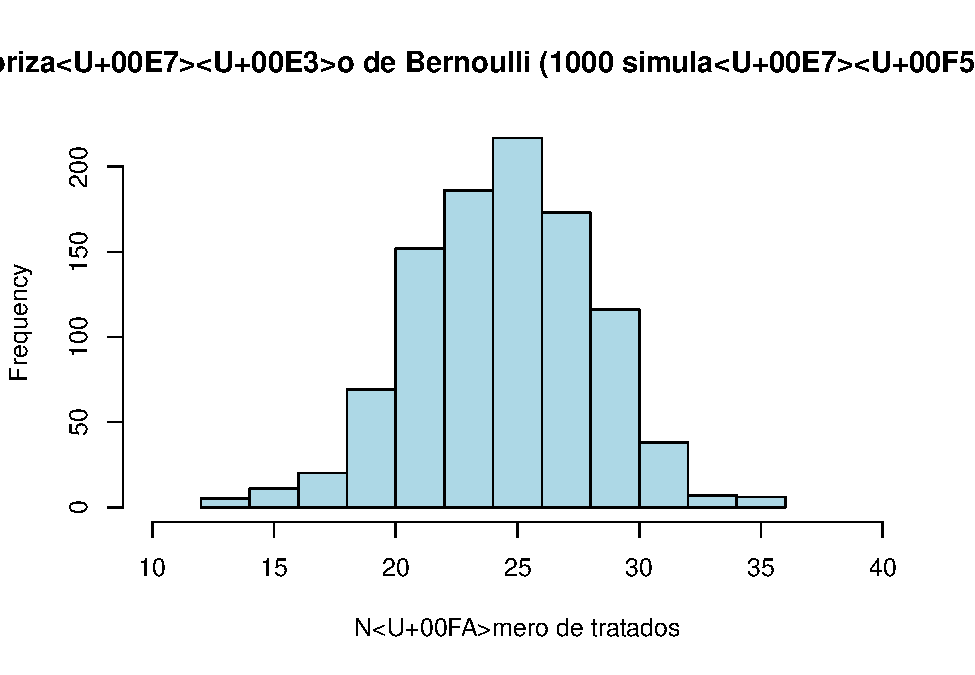
\includegraphics[keepaspectratio]{bookdownproj_files/figure-latex/bernoulli-1.pdf}}

A aleatorização de Bernoulli possui \(2^n\) configurações possíveis de alocação entre tratamento e controle.

\subsubsection{Aleatorização completa}\label{aleatorizauxe7uxe3o-completa}

Para evitar o problema do número variável de tratados, podemos fixar \emph{a priori} quantas unidades receberão o tratamento. Numeramos cada unidade de \(1\) a \(N\) e sorteamos \(m\) aleatoriamente para o tratamento; o restante vai para o controle.

Vantagem: garante o número de observações em cada grupo. Possui \(\binom{N}{m}\) configurações possíveis --- estamos descartando as aleatorizações ``indesejáveis'' (como todos no controle). O cálculo da variância é mais complexo que na aleatorização de Bernoulli.

\subsubsection{Aleatorização condicional (em bloco)}\label{aleatorizauxe7uxe3o-condicional-em-bloco}

Em muitos contextos, as unidades diferem em características pré-tratamento \(X\) que podem afetar o resultado. A \textbf{aleatorização em bloco} (\emph{block random assignment}) estratifica as unidades por \(X\) e aleatoriza separadamente dentro de cada estrato.

\textbf{Exemplo:} Em uma amostra de 100 pessoas, queremos 25 homens e 25 mulheres no tratamento. Sorteamos 25 homens para o tratamento (o restante vai para o controle) e, separadamente, 25 mulheres.

Formalmente, a aleatorização em bloco gera \textbf{permutabilidade condicional}: \(Y_i(1), Y_i(0) \perp D_i \mid X_i\). Isso é mais fraco que permutabilidade incondicional --- o tratamento não é independente dos resultados potenciais marginalmente, mas é independente \emph{dentro de cada estrato}.

Para estimar o ATE na população, calculamos o efeito dentro de cada bloco e ponderamos:

\[\hat{\tau}_{\text{ATE}} = \sum_{j=1}^{J} \frac{N_j}{N} \hat{\tau}_j\]

onde \(J\) é o número de blocos, \(N_j\) o tamanho do bloco \(j\), e \(\hat{\tau}_j\) o efeito estimado no bloco.

\textbf{Vantagens da aleatorização em bloco:}

\begin{itemize}
\tightlist
\item
  Pela Lei dos Grandes Números, tende a gerar \textbf{balanceamento} entre os grupos --- em variáveis observadas \emph{e} não-observadas dentro de cada bloco.
\item
  Em geral, \textbf{aumenta a precisão} (reduz o erro padrão), porque removemos parte da variância ao condicionar nos estratos.
\item
  A probabilidade de tratamento pode variar por bloco --- essa probabilidade é chamada de \emph{propensity score}.
\end{itemize}

\subsubsection{Precisão da aleatorização em bloco}\label{precisuxe3o-da-aleatorizauxe7uxe3o-em-bloco}

Vamos verificar o ganho de precisão com uma simulação. Criamos dois blocos com médias diferentes e comparamos o erro padrão da aleatorização simples com o da aleatorização em bloco.

\begin{Shaded}
\begin{Highlighting}[]
\CommentTok{\# Configuração: dois blocos com médias diferentes}
\NormalTok{n1 }\OtherTok{\textless{}{-}} \DecValTok{10}  \CommentTok{\# bloco 1}
\NormalTok{n2 }\OtherTok{\textless{}{-}} \DecValTok{16}  \CommentTok{\# bloco 2}
\NormalTok{N }\OtherTok{\textless{}{-}}\NormalTok{ n1 }\SpecialCharTok{+}\NormalTok{ n2}

\FunctionTok{set.seed}\NormalTok{(}\DecValTok{12}\NormalTok{)}
\NormalTok{y0 }\OtherTok{\textless{}{-}} \FunctionTok{c}\NormalTok{(}\FunctionTok{rnorm}\NormalTok{(n1, }\DecValTok{2}\NormalTok{, }\DecValTok{1}\NormalTok{), }\FunctionTok{rnorm}\NormalTok{(n2, }\DecValTok{6}\NormalTok{, }\DecValTok{1}\NormalTok{))  }\CommentTok{\# PO controle}
\NormalTok{y1 }\OtherTok{\textless{}{-}}\NormalTok{ y0 }\SpecialCharTok{+} \FloatTok{1.5}                               \CommentTok{\# PO tratamento (efeito = 1.5)}
\end{Highlighting}
\end{Shaded}

\begin{Shaded}
\begin{Highlighting}[]
\CommentTok{\# Aleatorização em bloco: metade de cada bloco para tratamento}
\NormalTok{t\_bloco1 }\OtherTok{\textless{}{-}} \FunctionTok{sample}\NormalTok{(}\DecValTok{1}\SpecialCharTok{:}\NormalTok{n1, n1}\SpecialCharTok{/}\DecValTok{2}\NormalTok{)}
\NormalTok{c\_bloco1 }\OtherTok{\textless{}{-}}\NormalTok{ (}\DecValTok{1}\SpecialCharTok{:}\NormalTok{n1)[}\SpecialCharTok{!}\NormalTok{(}\DecValTok{1}\SpecialCharTok{:}\NormalTok{n1 }\SpecialCharTok{\%in\%}\NormalTok{ t\_bloco1)]}
\NormalTok{t\_bloco2 }\OtherTok{\textless{}{-}} \FunctionTok{sample}\NormalTok{((n1}\SpecialCharTok{+}\DecValTok{1}\NormalTok{)}\SpecialCharTok{:}\NormalTok{(n1}\SpecialCharTok{+}\NormalTok{n2), n2}\SpecialCharTok{/}\DecValTok{2}\NormalTok{)}
\NormalTok{c\_bloco2 }\OtherTok{\textless{}{-}}\NormalTok{ ((n1}\SpecialCharTok{+}\DecValTok{1}\NormalTok{)}\SpecialCharTok{:}\NormalTok{(n1}\SpecialCharTok{+}\NormalTok{n2))[}\SpecialCharTok{!}\NormalTok{((n1}\SpecialCharTok{+}\DecValTok{1}\NormalTok{)}\SpecialCharTok{:}\NormalTok{(n1}\SpecialCharTok{+}\NormalTok{n2) }\SpecialCharTok{\%in\%}\NormalTok{ t\_bloco2)]}

\CommentTok{\# Resultados observados por bloco}
\NormalTok{y1\_obs\_bloco1 }\OtherTok{\textless{}{-}}\NormalTok{ y1[t\_bloco1]; y0\_obs\_bloco1 }\OtherTok{\textless{}{-}}\NormalTok{ y0[c\_bloco1]}
\NormalTok{y1\_obs\_bloco2 }\OtherTok{\textless{}{-}}\NormalTok{ y1[t\_bloco2]; y0\_obs\_bloco2 }\OtherTok{\textless{}{-}}\NormalTok{ y0[c\_bloco2]}

\CommentTok{\# Aleatorização simples (ignora blocos)}
\NormalTok{y1\_obs }\OtherTok{\textless{}{-}}\NormalTok{ y1[}\FunctionTok{c}\NormalTok{(t\_bloco1, t\_bloco2)]}
\NormalTok{y0\_obs }\OtherTok{\textless{}{-}}\NormalTok{ y0[}\FunctionTok{c}\NormalTok{(c\_bloco1, c\_bloco2)]}
\end{Highlighting}
\end{Shaded}

\begin{Shaded}
\begin{Highlighting}[]
\CommentTok{\# Erro padrão: aleatorização simples}
\NormalTok{ep\_simples }\OtherTok{\textless{}{-}} \FunctionTok{t.test}\NormalTok{(y1\_obs, y0\_obs)}\SpecialCharTok{$}\NormalTok{stderr}

\CommentTok{\# Erro padrão: aleatorização em bloco (ponderado)}
\NormalTok{ep1 }\OtherTok{\textless{}{-}} \FunctionTok{t.test}\NormalTok{(y1\_obs\_bloco1, y0\_obs\_bloco1)}\SpecialCharTok{$}\NormalTok{stderr}
\NormalTok{ep2 }\OtherTok{\textless{}{-}} \FunctionTok{t.test}\NormalTok{(y1\_obs\_bloco2, y0\_obs\_bloco2)}\SpecialCharTok{$}\NormalTok{stderr}
\NormalTok{ep\_bloco }\OtherTok{\textless{}{-}} \FunctionTok{sqrt}\NormalTok{(ep1}\SpecialCharTok{\^{}}\DecValTok{2} \SpecialCharTok{*}\NormalTok{ (n1}\SpecialCharTok{/}\NormalTok{N)}\SpecialCharTok{\^{}}\DecValTok{2} \SpecialCharTok{+}\NormalTok{ ep2}\SpecialCharTok{\^{}}\DecValTok{2} \SpecialCharTok{*}\NormalTok{ (n2}\SpecialCharTok{/}\NormalTok{N)}\SpecialCharTok{\^{}}\DecValTok{2}\NormalTok{)}

\CommentTok{\# Comparação}
\FunctionTok{data.frame}\NormalTok{(}
  \AttributeTok{Metodo =} \FunctionTok{c}\NormalTok{(}\StringTok{"Aleatorização simples"}\NormalTok{, }\StringTok{"Aleatorização em bloco"}\NormalTok{),}
  \AttributeTok{Erro\_Padrao =} \FunctionTok{round}\NormalTok{(}\FunctionTok{c}\NormalTok{(ep\_simples, ep\_bloco), }\DecValTok{4}\NormalTok{)}
\NormalTok{) }\SpecialCharTok{|\textgreater{}}
\NormalTok{  knitr}\SpecialCharTok{::}\FunctionTok{kable}\NormalTok{(}
    \AttributeTok{col.names =} \FunctionTok{c}\NormalTok{(}\StringTok{"Método"}\NormalTok{, }\StringTok{"Erro padrão"}\NormalTok{),}
    \AttributeTok{caption =} \StringTok{"Comparação de erros padrão"}
\NormalTok{  )}
\end{Highlighting}
\end{Shaded}

\begin{table}

\caption{\label{tab:bloco-compara}Compara<U+00E7><U+00E3>o de erros padr<U+00E3>o}
\centering
\begin{tabular}[t]{l|r}
\hline
M<U+00E9>todo & Erro padr<U+00E3>o\\
\hline
Aleatoriza<U+00E7><U+00E3>o simples & 0.9552\\
\hline
Aleatoriza<U+00E7><U+00E3>o em bloco & 0.3723\\
\hline
\end{tabular}
\end{table}

O erro padrão da aleatorização em bloco é substancialmente menor. A intuição: ao estratificar, eliminamos a variação \emph{entre} blocos (que é grande, pois os blocos têm médias diferentes) e ficamos apenas com a variação \emph{dentro} de cada bloco.

\subsubsection{Aleatorização por cluster}\label{aleatorizauxe7uxe3o-por-cluster}

Em alguns contextos, não é possível aleatorizar unidades individuais. Por exemplo, se o tratamento é um programa escolar, pode ser necessário aleatorizar \emph{escolas} inteiras --- todos os alunos de uma escola recebem o mesmo tratamento.

Nesse caso, a unidade de aleatorização é o \textbf{cluster} (escola), não a unidade de análise (aluno). No interior de cada cluster, todo mundo é tratado ou não-tratado: não há variação \emph{within}, apenas \emph{between}. Isso causa grande perda de variabilidade nos dados, reduzindo a precisão (aumento no erro padrão). Ainda assim, às vezes é a única aleatorização viável.

\subsection{Experimentos fatoriais}\label{experimentos-fatoriais}

Até aqui, consideramos experimentos com um único tratamento binário: cada unidade recebe \(D_i = 1\) ou \(D_i = 0\). Mas muitas perguntas de pesquisa envolvem \textbf{mais de um fator} simultaneamente. Um \textbf{experimento fatorial} é um desenho no qual duas ou mais variáveis de tratamento são manipuladas ao mesmo tempo, e todas as combinações de níveis são testadas.

\subsubsection{\texorpdfstring{Desenho \(2 \times 2\)}{Desenho 2 \textbackslash times 2}}\label{desenho-2-times-2}

O caso mais simples é o fatorial \(2 \times 2\): dois fatores, cada um com dois níveis. Suponha que queremos estudar o efeito de (1) um programa de tutoria (\(D_{1i} \in \{0,1\}\)) e (2) um incentivo financeiro (\(D_{2i} \in \{0,1\}\)) sobre o desempenho escolar. O desenho fatorial cruza os dois fatores, gerando quatro condições experimentais:

\begin{longtable}[]{@{}ccc@{}}
\toprule\noalign{}
Grupo & \(D_{1i}\) (tutoria) & \(D_{2i}\) (incentivo) \\
\midrule\noalign{}
\endhead
\bottomrule\noalign{}
\endlastfoot
1 & 0 & 0 \\
2 & 1 & 0 \\
3 & 0 & 1 \\
4 & 1 & 1 \\
\end{longtable}

A unidade \(i\) tem agora quatro resultados potenciais: \(Y_i(0,0)\), \(Y_i(1,0)\), \(Y_i(0,1)\) e \(Y_i(1,1)\). O resultado observado é \(Y_i = Y_i(D_{1i}, D_{2i})\).

\subsubsection{Efeitos principais e interações}\label{efeitos-principais-e-interauxe7uxf5es}

O desenho fatorial permite estimar três tipos de efeito causal:

\begin{enumerate}
\def\labelenumi{\arabic{enumi}.}
\tightlist
\item
  \textbf{Efeito principal do fator 1} (tutoria): a diferença média entre receber e não receber tutoria, \emph{averaged} sobre os níveis do incentivo:
\end{enumerate}

\[\tau_1 = \frac{1}{2}\Big[\mathbb{E}[Y_i(1,0) - Y_i(0,0)] + \mathbb{E}[Y_i(1,1) - Y_i(0,1)]\Big]\]

\begin{enumerate}
\def\labelenumi{\arabic{enumi}.}
\setcounter{enumi}{1}
\item
  \textbf{Efeito principal do fator 2} (incentivo): definido analogamente, \emph{averaged} sobre os níveis da tutoria.
\item
  \textbf{Efeito de interação}: mede se o efeito de um fator \emph{depende} do nível do outro:
\end{enumerate}

\[\tau_{12} = \mathbb{E}[Y_i(1,1) - Y_i(0,1)] - \mathbb{E}[Y_i(1,0) - Y_i(0,0)]\]

Se \(\tau_{12} = 0\), os efeitos dos dois fatores são aditivos --- cada fator opera independentemente do outro. Se \(\tau_{12} \neq 0\), há complementaridade (ou substituição) entre os tratamentos.

\subsubsection{Eficiência e generalização}\label{eficiuxeancia-e-generalizauxe7uxe3o}

Uma vantagem central do desenho fatorial é a \textbf{eficiência}: com a mesma amostra, estimamos os efeitos de múltiplos fatores. Em um desenho \(2 \times 2\) com \(N\) unidades, cada efeito principal usa \emph{todas} as \(N\) observações (comparando as \(N/2\) que receberam o fator com as \(N/2\) que não receberam), em vez de precisar de um experimento separado para cada fator.

O desenho generaliza para \(K\) fatores: um fatorial \(2^K\) tem \(2^K\) condições experimentais. À medida que \(K\) cresce, o número de condições cresce exponencialmente --- o que pode tornar o desenho inviável. No Cap. 5, veremos como os \textbf{experimentos conjoint} lidam com esse problema ao aleatorizar combinações de muitos fatores simultaneamente para cada respondente.

\subsection{Experimentos multi-arm}\label{experimentos-multi-arm}

Uma variação comum é o experimento \textbf{multi-arm} (\emph{multi-arm trial}): em vez de cruzar fatores independentes, a pesquisadora define \(K+1\) condições mutuamente exclusivas --- um controle e \(K\) tratamentos --- e cada unidade é alocada a exatamente uma delas. No Project STAR, por exemplo, alunos foram aleatorizados para turma regular (\(D_i = 0\)), turma pequena (\(D_i = 1\)) ou turma com assistente (\(D_i = 2\)) dentro de cada escola.

A diferença crucial em relação ao fatorial é que, no multi-arm, os tratamentos são \textbf{mutuamente exclusivos}: se \(D_i = 1\), então necessariamente \(D_i \neq 2\). No fatorial, os fatores são cruzados de forma independente --- uma unidade pode receber qualquer combinação.

A análise de um experimento multi-arm tipicamente envolve regredir o resultado em indicadores de cada braço:

\[Y_i = \alpha + \beta_1 X_{i1} + \beta_2 X_{i2} + \gamma W_i + U_i\]

onde \(X_{ik} = \mathbb{1}\{D_i = k\}\) e \(W_i\) são controles (por exemplo, indicadores de estrato). Com um único tratamento binário e aleatorização condicional, Angrist (\citeproc{ref-angrist1998}{1998}) mostrou que o coeficiente de regressão estima uma média convexa (com pesos positivos) de efeitos causais heterogêneos. No entanto, Goldsmith-Pinkham, Hull, and Kolesár (\citeproc{ref-goldsmith-pinkham2024}{2024}) demonstram que esse resultado \textbf{não se generaliza} para múltiplos tratamentos.

O problema é o \textbf{contamination bias}: quando os tratamentos são mutuamente exclusivos, o resíduo da projeção de \(X_{i1}\) sobre os controles e os demais tratamentos não é \emph{mean-independent} de \(X_{i2}\), mesmo que ambos sejam aleatorizados condicionalmente em \(W_i\). O coeficiente \(\beta_1\) passa a incorporar não só o efeito de \(D_i = 1\), mas também uma média --- com pesos que somam zero e podem ser negativos --- dos efeitos dos outros tratamentos. Formalmente:

\[\beta_1 = \underbrace{\mathbb{E}[\lambda_{11}(W_i)\tau_1(W_i)]}_{\text{efeito próprio}} + \underbrace{\mathbb{E}[\lambda_{12}(W_i)\tau_2(W_i)]}_{\text{contaminação}}\]

onde \(\tau_k(w) = \mathbb{E}[Y_i(k) - Y_i(0) \mid W_i = w]\) são os efeitos causais condicionais, \(\lambda_{11}\) são pesos próprios (convexos), e \(\lambda_{12}\) são pesos de contaminação que somam zero.

Duas condições são \textbf{necessárias} para que o contamination bias seja relevante:

\begin{enumerate}
\def\labelenumi{\arabic{enumi}.}
\item
  \textbf{Heterogeneidade nos efeitos} dos outros tratamentos: se \(\tau_2(w)\) é constante em \(w\), a covariância com os pesos \(\lambda_{12}\) é zero e o viés desaparece.
\item
  \textbf{Variação nos propensity scores} entre estratos: se a probabilidade de cada tratamento é a mesma em todos os estratos, os pesos de contaminação são zero.
\end{enumerate}

Em experimentos fatoriais com aleatorização independente dos fatores, o contamination bias não surge --- precisamente porque a independência entre fatores elimina a dependência não-linear que gera o problema. Mas em desenhos multi-arm estratificados, onde as probabilidades de alocação variam por estrato, o viés pode ser substantivo, mesmo com aleatorização perfeita dentro de cada estrato.

\subsection{Planejando experimentos com DeclareDesign}\label{planejando-experimentos-com-declaredesign}

Uma ferramenta útil para planejar e diagnosticar experimentos é o pacote \texttt{DeclareDesign} (\citeproc{ref-blair2023}{Blair, Coppock, and Humphreys 2023}). O framework é baseado no acrônimo \textbf{MIDA}: \emph{Models} (modelo dos resultados potenciais), \emph{Inquiries} (estimando), \emph{Data strategies} (estratégia de dados/aleatorização) e \emph{Answer strategies} (estimador).

Vamos declarar um experimento simples com dois braços (\emph{two-arm trial}):

\begin{Shaded}
\begin{Highlighting}[]
\FunctionTok{library}\NormalTok{(DeclareDesign)}

\CommentTok{\# 1. Modelo: 500 unidades, covariável X, efeito de 0.2}
\NormalTok{model }\OtherTok{\textless{}{-}} \FunctionTok{declare\_model}\NormalTok{(}
  \AttributeTok{N =} \DecValTok{500}\NormalTok{,}
  \AttributeTok{X =} \FunctionTok{rep}\NormalTok{(}\FunctionTok{c}\NormalTok{(}\DecValTok{0}\NormalTok{, }\DecValTok{1}\NormalTok{), }\AttributeTok{each =}\NormalTok{ N }\SpecialCharTok{/} \DecValTok{2}\NormalTok{),}
  \AttributeTok{U =} \FunctionTok{rnorm}\NormalTok{(N, }\AttributeTok{sd =} \FloatTok{0.25}\NormalTok{),}
  \FunctionTok{potential\_outcomes}\NormalTok{(Y }\SpecialCharTok{\textasciitilde{}} \FloatTok{0.2} \SpecialCharTok{*}\NormalTok{ Z }\SpecialCharTok{+}\NormalTok{ X }\SpecialCharTok{+}\NormalTok{ U)}
\NormalTok{)}

\CommentTok{\# 2. Estimando: ATE}
\NormalTok{inquiry }\OtherTok{\textless{}{-}} \FunctionTok{declare\_inquiry}\NormalTok{(}\AttributeTok{ATE =} \FunctionTok{mean}\NormalTok{(Y\_Z\_1 }\SpecialCharTok{{-}}\NormalTok{ Y\_Z\_0))}

\CommentTok{\# 3. Estratégia de dados: aleatorização completa (250 tratados)}
\NormalTok{data\_strategy }\OtherTok{\textless{}{-}} \FunctionTok{declare\_assignment}\NormalTok{(}\AttributeTok{Z =} \FunctionTok{complete\_ra}\NormalTok{(}\AttributeTok{N =}\NormalTok{ N, }\AttributeTok{m =} \DecValTok{250}\NormalTok{)) }\SpecialCharTok{+}
  \FunctionTok{declare\_measurement}\NormalTok{(}\AttributeTok{Y =} \FunctionTok{reveal\_outcomes}\NormalTok{(Y }\SpecialCharTok{\textasciitilde{}}\NormalTok{ Z))}

\CommentTok{\# 4. Estimador: diferença de médias via regressão}
\NormalTok{estimator }\OtherTok{\textless{}{-}} \FunctionTok{declare\_estimator}\NormalTok{(Y }\SpecialCharTok{\textasciitilde{}}\NormalTok{ Z, }\AttributeTok{inquiry =} \StringTok{"ATE"}\NormalTok{)}

\CommentTok{\# Combinando tudo}
\NormalTok{two\_arm\_trial }\OtherTok{\textless{}{-}}\NormalTok{ model }\SpecialCharTok{+}\NormalTok{ inquiry }\SpecialCharTok{+}\NormalTok{ data\_strategy }\SpecialCharTok{+}\NormalTok{ estimator}
\end{Highlighting}
\end{Shaded}

Cada componente corresponde a uma letra do MIDA. A função \texttt{declare\_model} especifica a população e os resultados potenciais; \texttt{declare\_inquiry} define o estimando (ATE); \texttt{declare\_assignment} e \texttt{declare\_measurement} descrevem a aleatorização e a switching equation; e \texttt{declare\_estimator} especifica como estimamos o efeito.

Podemos simular dados do desenho:

\begin{Shaded}
\begin{Highlighting}[]
\FunctionTok{head}\NormalTok{(}\FunctionTok{draw\_data}\NormalTok{(two\_arm\_trial), }\DecValTok{10}\NormalTok{)}
\end{Highlighting}
\end{Shaded}

\begin{verbatim}
##     ID X           U       Y_Z_0      Y_Z_1 Z          Y
## 1  001 0  0.17975340  0.17975340 0.37975340 1 0.37975340
## 2  002 0  0.14184465  0.14184465 0.34184465 0 0.14184465
## 3  003 0 -0.07395336 -0.07395336 0.12604664 1 0.12604664
## 4  004 0  0.41948484  0.41948484 0.61948484 0 0.41948484
## 5  005 0  0.13238069  0.13238069 0.33238069 1 0.33238069
## 6  006 0  0.22464800  0.22464800 0.42464800 1 0.42464800
## 7  007 0  0.29101108  0.29101108 0.49101108 1 0.49101108
## 8  008 0 -0.17435610 -0.17435610 0.02564390 1 0.02564390
## 9  009 0 -0.15919449 -0.15919449 0.04080551 1 0.04080551
## 10 010 0  0.29106704  0.29106704 0.49106704 1 0.49106704
\end{verbatim}

E diagnosticar o desenho --- verificando viés, erro padrão, poder e cobertura:

\begin{Shaded}
\begin{Highlighting}[]
\FunctionTok{diagnose\_design}\NormalTok{(two\_arm\_trial, }\AttributeTok{sims =} \DecValTok{100}\NormalTok{)}
\end{Highlighting}
\end{Shaded}

\begin{verbatim}
## 
## Research design diagnosis based on 100 simulations. Diagnosis completed in 1 secs. Diagnosand estimates with bootstrapped standard errors in parentheses (100 replicates).
## 
##         Design Inquiry Estimator Outcome Term N Sims Mean Estimand
##  two_arm_trial     ATE estimator       Y    Z    100          0.20
##                                                             (0.00)
##  Mean Estimate   Bias SD Estimate   RMSE  Power Coverage
##           0.20  -0.00        0.04   0.04   0.99     0.98
##         (0.00) (0.00)      (0.00) (0.00) (0.01)   (0.01)
\end{verbatim}

Também podemos comparar o desempenho com diferentes tamanhos de amostra:

\begin{Shaded}
\begin{Highlighting}[]
\NormalTok{designs }\OtherTok{\textless{}{-}} \FunctionTok{redesign}\NormalTok{(two\_arm\_trial, }\AttributeTok{N =} \FunctionTok{c}\NormalTok{(}\DecValTok{100}\NormalTok{, }\DecValTok{200}\NormalTok{, }\DecValTok{300}\NormalTok{, }\DecValTok{400}\NormalTok{, }\DecValTok{500}\NormalTok{))}
\FunctionTok{diagnose\_design}\NormalTok{(designs)}
\end{Highlighting}
\end{Shaded}

\begin{verbatim}
## 
## Research design diagnosis based on 500 simulations. Diagnosis completed in 7 secs. Diagnosand estimates with bootstrapped standard errors in parentheses (100 replicates).
## 
##    Design   N Inquiry Estimator Outcome Term N Sims Mean Estimand Mean Estimate
##  design_1 100     ATE estimator       Y    Z    500          0.20          0.20
##                                                            (0.00)        (0.00)
##  design_2 200     ATE estimator       Y    Z    500          0.20          0.20
##                                                            (0.00)        (0.00)
##  design_3 300     ATE estimator       Y    Z    500          0.20          0.20
##                                                            (0.00)        (0.00)
##  design_4 400     ATE estimator       Y    Z    500          0.20          0.20
##                                                            (0.00)        (0.00)
##  design_5 500     ATE estimator       Y    Z    500          0.20          0.20
##                                                            (0.00)        (0.00)
##    Bias SD Estimate   RMSE  Power Coverage
##    0.00        0.05   0.05   0.98     0.95
##  (0.00)      (0.00) (0.00) (0.01)   (0.01)
##   -0.00        0.05   0.05   0.98     0.97
##  (0.00)      (0.00) (0.00) (0.01)   (0.01)
##   -0.00        0.05   0.05   0.97     0.94
##  (0.00)      (0.00) (0.00) (0.01)   (0.01)
##    0.00        0.05   0.05   0.98     0.96
##  (0.00)      (0.00) (0.00) (0.01)   (0.01)
##   -0.00        0.05   0.05   0.97     0.94
##  (0.00)      (0.00) (0.00) (0.01)   (0.01)
\end{verbatim}

\subsection{Resumo e próximos passos}\label{resumo-e-pruxf3ximos-passos-3}

Neste capítulo, vimos como experimentos aleatórios eliminam o viés de seleção:

\begin{enumerate}
\def\labelenumi{\arabic{enumi}.}
\item
  \textbf{Permutabilidade.} A aleatorização garante que tratamento e controle sejam comparáveis em esperança, tornando a SDO um estimador não-viesado do ATE.
\item
  \textbf{Restrição de exclusão.} Além da aleatorização, precisamos que o resultado dependa do tratamento \emph{recebido}, não da alocação. Duplo cego e paralelismo na administração ajudam a garantir essa condição.
\item
  \textbf{Tipos de aleatorização.} Bernoulli, completa, em bloco e por cluster --- cada qual com vantagens e limitações. A aleatorização em bloco tende a aumentar a precisão; a por cluster, a reduzi-la.
\item
  \textbf{DeclareDesign.} Permite planejar, simular e diagnosticar um desenho experimental antes de conduzi-lo, avaliando poder, viés e cobertura.
\end{enumerate}

Ao longo do capítulo, supusemos condições ideais: sem \emph{attrition} e com \emph{compliance} perfeito. Nos próximos capítulos, veremos o que acontece quando não temos aleatorização e precisamos recorrer a estratégias observacionais.

\subsection{Exercícios}\label{exercuxedcios-1}

\subsubsection{Exercício 1: Cartões-postais e participação eleitoral}\label{exercuxedcio-1-cartuxf5es-postais-e-participauxe7uxe3o-eleitoral}

Você conduz um experimento aleatório para testar o efeito de um cartão-postal sobre a participação eleitoral, sorteando independentemente uma moeda para cada sujeito com probabilidade \(0 < p < 1\) de receber o tratamento. Assuma SUTVA. Você estima o seguinte modelo por MQO:

\[Y_i = \beta_0 + \beta_1 D_i + \beta_2 S_i + \beta_3 D_i S_i + u_i\]

em que \(Y_i\) indica se o indivíduo votou, \(D_i\) é o indicador de tratamento, \(S_i\) indica se o indivíduo vive em um estado competitivo (\emph{battleground state}), e \(D_i S_i\) é a interação.

\begin{enumerate}
\def\labelenumi{(\alph{enumi})}
\item
  Interprete os quatro coeficientes \(\beta\).
\item
  Como testar a hipótese de que o efeito do tratamento é igual entre os dois tipos de estado?
\end{enumerate}

\subsubsection{Exercício 2: Anúncios de TV e participação eleitoral}\label{exercuxedcio-2-anuxfancios-de-tv-e-participauxe7uxe3o-eleitoral}

Você quer testar se anúncios de TV aumentam a participação eleitoral. O experimento pode ser conduzido em até 16 mercados de mídia, dos quais até 8 podem ser sorteados para o tratamento. Os anúncios só podem ser exibidos para o mercado de mídia como um todo. Você tem informações individuais para todos os eleitores: mercado, idade, sexo, raça/etnia e participação nas duas eleições anteriores.

\begin{enumerate}
\def\labelenumi{(\alph{enumi})}
\item
  Como alocar aleatoriamente os mercados ao tratamento?
\item
  Como analisar esse experimento? Em que nível deve ser feita a análise?
\end{enumerate}

\subsubsection{Exercício 3: Exclusão de participantes em experimentos de survey}\label{exercuxedcio-3-exclusuxe3o-de-participantes-em-experimentos-de-survey}

Pesquisadores às vezes excluem participantes de um experimento de survey por: (1) não passarem em uma checagem de atenção pré-tratamento; (2) não passarem em uma checagem de atenção pós-tratamento; (3) completarem o survey muito rapidamente.

\begin{enumerate}
\def\labelenumi{(\alph{enumi})}
\item
  Se o interesse é no efeito médio do tratamento \textbf{entre os sujeitos que não foram excluídos}, qual dessas estratégias é não-viesada?
\item
  Se o interesse é no efeito médio do tratamento \textbf{entre todos os participantes que iniciaram o experimento}, qual dessas estratégias é não-viesada?
\end{enumerate}

\section{Experimentos de Survey}\label{experimentos-de-survey}

\subsection{Introdução}\label{introduuxe7uxe3o-3}

\textbf{Objetivos de aprendizado:}

\begin{enumerate}
\def\labelenumi{\arabic{enumi}.}
\tightlist
\item
  Avaliar os usos e limitações dos principais paradigmas de experimentos de survey
\item
  Identificar questões práticas que surgem na implementação de experimentos e avaliar como antecipá-las e respondê-las
\item
  Avaliar as forças, fraquezas e questões éticas de experimentos como desenho de pesquisa e método de avaliação
\end{enumerate}

Experimentos de survey combinam o controle experimental da aleatorização com o alcance dos surveys amostrais. Os respondentes são aleatoriamente designados a diferentes condições experimentais (formulações distintas de perguntas, vinhetas com informações variadas, perfis com atributos sorteados) e as diferenças nas respostas entre os grupos são atribuídas ao efeito causal do tratamento.

A lógica é idêntica à do Cap. 4: a aleatorização garante permutabilidade e elimina o viés de seleção. A diferença é o contexto de aplicação. Em um experimento de campo, o tratamento é uma intervenção no mundo real: um programa social, um cartão enviado a eleitores, um incentivo financeiro. Em um experimento de survey, o tratamento é \emph{informacional}: uma diferença no texto lido pelo respondente, nos atributos de um perfil avaliado, ou na ordem das perguntas. Experimentos de survey são mais rápidos, baratos e fáceis de implementar. Mas essa conveniência levanta questões sobre se as respostas refletem atitudes e comportamentos reais.

\subsection{Origem, história e evolução dos experimentos de survey}\label{origem-histuxf3ria-e-evoluuxe7uxe3o-dos-experimentos-de-survey}

A história dos experimentos de survey começa na década de 1940, quando pesquisadores de opinião pública descobriram que pequenas mudanças na formulação de perguntas podiam produzir grandes diferenças nas respostas. Cantril (\citeproc{ref-cantril1940}{1940}) conduziu um dos primeiros experimentos sistemáticos de formulação (\emph{wording experiments}), usando o método \emph{split-ballot}: duas amostras probabilísticas de cerca de 1.550 pessoas cada receberam versões ligeiramente diferentes da mesma pergunta, em março de 1940. Uma das perguntas testava se mencionar Hitler alterava o apoio dos americanos a ajudar a Inglaterra e a França:

\begin{longtable}[]{@{}
  >{\raggedright\arraybackslash}p{(\linewidth - 6\tabcolsep) * \real{0.2264}}
  >{\centering\arraybackslash}p{(\linewidth - 6\tabcolsep) * \real{0.2264}}
  >{\centering\arraybackslash}p{(\linewidth - 6\tabcolsep) * \real{0.3019}}
  >{\centering\arraybackslash}p{(\linewidth - 6\tabcolsep) * \real{0.2453}}@{}}
\toprule\noalign{}
\begin{minipage}[b]{\linewidth}\raggedright
Formulação
\end{minipage} & \begin{minipage}[b]{\linewidth}\centering
Fazer mais
\end{minipage} & \begin{minipage}[b]{\linewidth}\centering
Não fazer mais
\end{minipage} & \begin{minipage}[b]{\linewidth}\centering
Sem opinião
\end{minipage} \\
\midrule\noalign{}
\endhead
\bottomrule\noalign{}
\endlastfoot
``Os EUA deveriam fazer mais para ajudar a Inglaterra e a França?'' & 13\% & 75\% & 12\% \\
``Os EUA deveriam fazer mais para ajudar a Inglaterra e a França \emph{na luta contra Hitler}?'' & 22\% & 66\% & 12\% \\
\end{longtable}

Adicionar ``na luta contra Hitler'' aumentou o apoio a fazer mais de 13\% para 22\% (nove pontos percentuais), sem alterar a proporção sem opinião. A menção a um inimigo concreto transformou uma questão abstrata sobre política externa em uma questão sobre combater uma ameaça identificável. Cantril interpretou o resultado como evidência de que a consciência de um inimigo a ser derrotado, além de aliados a serem ajudados, intensificou o desejo de uma vitória Aliada.

No mesmo estudo, Cantril testou o efeito de mencionar o presidente Roosevelt na aprovação da visita de Sumner Welles a capitais europeias: a aprovação se manteve em 43\% nas duas versões, mas a desaprovação subiu de 25\% para 31\% quando Roosevelt era mencionado como responsável, e a proporção sem opinião caiu de 32\% para 26\%. O nome do presidente trouxe pessoas da categoria ``sem opinião'' para a desaprovação.

Outro resultado clássico da mesma época é o de Rugg (\citeproc{ref-rugg1941}{1941}): perguntando se os EUA deveriam ``proibir'' (\emph{forbid}) discursos contra a democracia, 54\% disseram sim; perguntando se deveriam ``não permitir'' (\emph{not allow}) os mesmos discursos, 75\% disseram sim, apesar de as duas formulações serem logicamente equivalentes. Esses achados estabeleceram que a forma da pergunta era tão importante quanto seu conteúdo.

Esses achados iniciais eram essencialmente descritivos: documentavam a sensibilidade das respostas à formulação, mas sem uma teoria sistemática sobre por que e quando os efeitos ocorriam. O método usado era o \textbf{split-ballot} (ou \emph{split-half}): a mesma amostra era dividida aleatoriamente em dois grupos, cada um recebendo uma versão diferente da pergunta. É o desenho experimental mais simples possível, e continua sendo a base de muitos experimentos de survey contemporâneos.

O avanço teórico veio nas décadas seguintes. Schuman and Presser (\citeproc{ref-schuman1981}{1981}) catalogaram sistematicamente os efeitos de formulação, ordem de perguntas, formato de resposta e outras características do instrumento de survey. A contribuição central foi demonstrar que esses efeitos eram padrões replicáveis que obedeciam a princípios cognitivos, não idiossincrasias de amostras específicas. Por exemplo, o efeito \emph{forbid/allow} reflete uma assimetria linguística: ``proibir'' evoca uma ação mais forte e autoritária do que ``não permitir'', mesmo que o resultado prático seja idêntico.

Paralelamente, a psicologia cognitiva ofereceu os mecanismos explicativos. Tourangeau, Rips, and Rasinski (\citeproc{ref-tourangeau2000}{2000}) formalizaram um modelo do processo de resposta a surveys em quatro etapas: (1) \textbf{compreensão} da pergunta, (2) \textbf{recuperação} de informações relevantes da memória, (3) \textbf{julgamento} e integração dessas informações, e (4) \textbf{formatação} da resposta para se adequar às opções oferecidas. Experimentos de survey podem intervir em qualquer uma dessas etapas: um \emph{framing experiment} altera a compreensão; um \emph{priming experiment} afeta a recuperação; a escala de resposta afeta a formatação. Esse modelo tornou possível \emph{prever} efeitos de desenho, não apenas documentá-los post hoc.

A partir dos anos 1990, duas transformações expandiram o alcance dos experimentos de survey. Primeiro, a revolução tecnológica: surveys assistidos por computador (CATI, CAPI, CAWI) tornaram possível aleatorizar tratamentos automaticamente, sem depender de versões impressas diferentes do questionário. Segundo, o trabalho de Paul Sniderman e colegas demonstrou que experimentos de survey podiam testar \emph{teorias} sobre como cidadãos formam opiniões políticas, não apenas documentar efeitos de formulação (\citeproc{ref-sniderman2011handbook}{Sniderman and Druckman 2011}). Experimentos de survey passaram a testar hipóteses causais sobre os determinantes das atitudes. Um exemplo influente é o \emph{multi-investigator study} de Sniderman: em vez de um único fator (formulação A vs.~B), o desenho cruza múltiplos fatores (raça do alvo, tipo de política, enquadramento) para testar predições teóricas específicas.

A partir dos anos 2010, o crescimento de plataformas online (Amazon Mechanical Turk, Prolific, Lucid) e painéis amostrais (YouGov, LISS) reduziu dramaticamente o custo e o tempo de implementação. Mullinix et al. (\citeproc{ref-mullinix2015}{2015}) mostraram que os efeitos experimentais estimados em amostras de conveniência (MTurk) são notavelmente similares aos obtidos em amostras probabilísticas nacionais. Embora os níveis absolutos das variáveis possam diferir, os \emph{efeitos do tratamento} tendem a ser replicáveis. Essa evidência abriu caminho para a proliferação de experimentos de survey em ciência política, relações internacionais e políticas públicas.

Hoje, experimentos de survey são um dos métodos mais utilizados em ciência política empírica. Mutz (\citeproc{ref-mutz2011}{2011}) oferece o tratamento de referência sobre \emph{population-based survey experiments}: experimentos conduzidos em amostras probabilísticas da população, que combinam validade interna (aleatorização) com validade externa (generalização para a população amostrada).

\subsection{Usos de experimentos de survey}\label{usos-de-experimentos-de-survey}

Experimentos de survey servem a quatro grandes propósitos na pesquisa em ciências sociais.

\textbf{1. Testar teorias causais sobre formação de atitudes.} O uso mais ambicioso é testar hipóteses sobre \emph{como} e \emph{por que} cidadãos formam opiniões. O modelo canônico é o de Zaller (\citeproc{ref-zaller1992}{1992}): a opinião expressa em um survey é função de (a) quais considerações estão acessíveis na memória no momento da pergunta, e (b) como essas considerações são integradas em uma resposta. Experimentos de survey manipulam diretamente a acessibilidade (via priming) ou o enquadramento (via framing) para testar predições derivadas desse e de outros modelos teóricos.

\textbf{2. Mensurar atitudes sensíveis.} Quando perguntas diretas produzem respostas socialmente desejáveis (sobre preconceito racial, corrupção, comportamento ilegal, apoio a grupos extremistas), técnicas como list experiments e endorsement experiments permitem estimar a prevalência da atitude sem que nenhum respondente individual revele sua posição. Em contextos autoritários ou semiautoritários, onde a desejabilidade social e o medo de represálias distorcem severamente as respostas, essas técnicas são especialmente valiosas.

\textbf{3. Estudar o impacto de elementos comunicativos.} Como a forma de apresentar uma questão política afeta o apoio público? Framing experiments e priming experiments manipulam sistematicamente a apresentação da informação para isolar o efeito causal de enquadramentos específicos. Esse tipo de estudo é diretamente relevante para entender a comunicação política, o efeito da mídia e a formação da agenda pública.

\textbf{4. Avaliar preferências multidimensionais.} Quando decisões envolvem múltiplos atributos (votar em um candidato, aceitar um imigrante, apoiar uma política pública), conjoint experiments permitem estimar a importância causal de cada dimensão. A seção dedicada a conjoint neste capítulo detalha esse uso.

Gaines, Kuklinski, and Quirk (\citeproc{ref-gaines2007}{2007}) enfatizam a distinção entre experimentos de survey usados para \textbf{identificação causal} e experimentos usados como \textbf{ferramentas de mensuração}. No primeiro caso, o objetivo é estimar o efeito de um tratamento sobre uma atitude ou comportamento, e a validade depende da aleatorização. No segundo, o objetivo é medir com mais precisão uma atitude que perguntas diretas não captam bem, e a validade depende de suposições sobre o mecanismo de resposta (como a suposição de ``no design effect'' em list experiments). Os dois usos enfrentam ameaças diferentes e requerem desenhos distintos.

\subsection{Metodologia de survey}\label{metodologia-de-survey}

Experimentos de survey herdam os problemas metodológicos de surveys convencionais e acrescentam alguns próprios. Antes de discutir os tipos específicos de experimentos, revisamos brevemente as questões metodológicas que afetam qualquer survey e como elas interagem com o componente experimental.

\textbf{Efeitos de formulação.} Como vimos na seção histórica, a escolha de palavras afeta as respostas. A distinção \emph{forbid/not allow} é o caso clássico, mas efeitos de formulação são ubíquos: perguntar sobre ``mudança climática'' vs.~``aquecimento global'' produz respostas diferentes; perguntar sobre ``assistência social'' vs.~``ajuda aos pobres'' também. Para o experimentalista, a implicação é que o texto exato do tratamento importa e deve ser reportado integralmente, não apenas resumido.

\textbf{Efeitos de ordem.} A sequência em que perguntas são apresentadas pode afetar as respostas. Perguntas anteriores ativam certas considerações na memória (\emph{carryover effects}), que influenciam as respostas subsequentes. Em um experimento de survey, efeitos de ordem podem contaminar o tratamento se as perguntas contextuais não forem controladas. A solução padrão é aleatorizar a ordem das perguntas não experimentais.

\textbf{Efeitos de escala.} O formato das opções de resposta (escala de 5 ou 7 pontos, rótulos verbais ou numéricos, inclusão de ponto médio) afeta a distribuição das respostas. Em comparações entre condições experimentais, esses efeitos são constantes (ambos os grupos usam a mesma escala) e portanto não viesam as estimativas. Mas se o pesquisador quer comparar resultados entre surveys com escalas diferentes, a interpretação se complica.

\textbf{Satisficing.} Krosnick (\citeproc{ref-krosnick1991}{1991}) introduziu o conceito de \emph{survey satisficing}: em vez de processar cuidadosamente cada pergunta (\emph{optimizing}), respondentes com baixa motivação ou capacidade cognitiva adotam atalhos. Escolhem a primeira opção aceitável, respondem no ponto médio, ou seguem padrões repetitivos. Para experimentos de survey, o satisficing atenua os efeitos do tratamento em direção a zero, pois respondentes que não processam o estímulo experimental respondem como se estivessem no grupo de controle. O problema é especialmente relevante em surveys longos e em amostras com grande variação em escolaridade, como as amostras probabilísticas da população brasileira.

\textbf{Desejabilidade social.} Respondentes tendem a dar respostas que os façam parecer ``bons'': menos preconceituosos, mais informados, mais participativos. Em um experimento de survey, a desejabilidade social pode interagir com o tratamento. Se o tratamento torna mais saliente uma norma social (ex: ``especialistas dizem que X é racismo''), a resposta pode refletir conformidade à norma e não uma mudança genuína de atitude. Técnicas indiretas de mensuração (list experiments, endorsement experiments) foram desenvolvidas para contornar esse problema.

\subsection{Mensuração e temas sensíveis}\label{mensurauxe7uxe3o-e-temas-sensuxedveis}

Uma das contribuições mais importantes dos experimentos de survey é oferecer ferramentas para medir atitudes e comportamentos que respondentes não revelam quando perguntados diretamente. A lógica geral é substituir a pergunta direta por um desenho experimental que permite estimar a prevalência da atitude sensível \emph{na amostra} sem identificar qual respondente individual a possui.

\textbf{O problema.} Considere a pergunta: ``Você já pagou propina a um funcionário público?''. A resposta honesta pode ter consequências sociais ou legais. O resultado previsível é subreporte: a proporção que responde ``sim'' subestima a prevalência real. Esse viés de desejabilidade social (\emph{social desirability bias}) é sistemático, não aleatório, e portanto não se cancela com amostras maiores.

\textbf{Resposta aleatorizada (randomized response).} A técnica mais antiga para temas sensíveis foi proposta por Warner (\citeproc{ref-warner1965}{1965}). O respondente usa um mecanismo aleatório (um dado, uma moeda) para decidir se responde a pergunta sensível ou a uma pergunta inocente, sem que o entrevistador saiba qual pergunta foi respondida. Por exemplo: ``Lance um dado em segredo. Se cair 1, responda `sim' independentemente da sua opinião. Se cair 2 a 6, responda honestamente: você já pagou propina?'' Como o entrevistador não sabe o resultado do dado, a resposta individual é protegida. Mas, conhecendo a probabilidade do mecanismo (\(1/6\)), o pesquisador pode estimar a proporção verdadeira na amostra por álgebra simples.

Seja \(p\) a proporção verdadeira que pagou propina e \(\pi = P(\text{sim observado})\) a proporção observada de respostas ``sim''. Pelo mecanismo descrito: \(\pi = \frac{1}{6} \cdot 1 + \frac{5}{6} \cdot p\), logo \(p = \frac{6\pi - 1}{5}\). O custo é eficiência: os erros padrão são substancialmente maiores do que com perguntas diretas, pois parte da variação nas respostas vem do mecanismo aleatório, não da atitude.

\textbf{List experiments (técnica de contagem de itens).} Uma alternativa mais moderna, que será detalhada na seção sobre tipos de experimentos, é o list experiment. O respondente recebe uma lista de itens e reporta apenas \emph{quantos} se aplicam a ele, não \emph{quais}. O grupo de tratamento recebe um item sensível adicional. A diferença entre as médias dos grupos estima a proporção que endossa o item sensível. A vantagem sobre a resposta aleatorizada é que o procedimento é mais intuitivo para o respondente e não requer mecanismos externos.

\textbf{Endorsement experiments.} Quando o tema sensível envolve apoio a um grupo ou ator (partidos extremistas, grupos armados, movimentos ilegais), endorsement experiments atribuem o endosso de uma política a diferentes atores e medem a diferença na aprovação da política. Se a aprovação muda quando o ator muda, a diferença captura o efeito do ator (positivo ou negativo). Esse desenho será detalhado adiante.

A escolha entre essas técnicas depende do contexto. Resposta aleatorizada é mais adequada para comportamentos binários bem definidos (pagou/não pagou propina). List experiments são flexíveis e intuitivos, mas requerem amostras grandes. Endorsement experiments são específicos para atitudes em relação a atores ou grupos.

\subsection{Identificação causal}\label{identificauxe7uxe3o-causal}

A identificação causal em experimentos de survey segue a mesma lógica do Cap. 4. Usando a notação de resultados potenciais, cada respondente \(i\) tem dois resultados potenciais: \(Y_i(1)\) (resposta sob tratamento) e \(Y_i(0)\) (resposta sob controle). O efeito causal individual é \(\tau_i = Y_i(1) - Y_i(0)\), e o estimando de interesse é tipicamente o ATE: \(\tau = \mathbb{E}[Y_i(1) - Y_i(0)]\).

\textbf{Aleatorização.} Em um experimento de survey, o tratamento \(D_i\) é aleatorizado pelo software do survey: cada respondente é designado a uma condição com probabilidade conhecida. Isso garante \(Y_i(1), Y_i(0) \perp D_i\) (permutabilidade), e a simples diferença de médias identifica o ATE sem viés.

\textbf{SUTVA.} A suposição de não interferência (SUTVA) é tipicamente plausível em surveys: respondentes são entrevistados isoladamente e não observam as respostas uns dos outros. A exceção são surveys em domicílios, onde um respondente pode discutir as perguntas com familiares antes de o próximo ser entrevistado. Em surveys online, a não interferência é quase automática.

\textbf{O que é o ``tratamento''?} Nos experimentos de survey, o tratamento é informacional, não comportamental. O respondente \emph{lê} algo diferente; ele não \emph{experimenta} algo diferente em sua vida. O efeito estimado captura como a informação fornecida pelo experimento afeta a resposta. Essa mudança pode envolver uma alteração genuína de atitude, a ativação de uma atitude preexistente, ou uma resposta mecânica à informação recebida. Gaines, Kuklinski, and Quirk (\citeproc{ref-gaines2007}{2007}) alertam que é fácil confundir esses mecanismos. O experimento identifica o efeito da \emph{informação fornecida}, não necessariamente o efeito da \emph{realidade} que a informação descreve.

\textbf{Validade interna vs.~validade externa.} A validade interna (a capacidade de atribuir a diferença observada ao tratamento) é garantida pela aleatorização, como em qualquer experimento. A validade externa (a capacidade de generalizar os resultados para além da amostra e do contexto) é a questão mais debatida. Mutz (\citeproc{ref-mutz2011}{2011}) argumenta que \emph{population-based survey experiments}, conduzidos em amostras probabilísticas, resolvem parcialmente o problema: os efeitos são internamente válidos \emph{e} estimados para uma população definida. Mullinix et al. (\citeproc{ref-mullinix2015}{2015}) complementam mostrando que, na prática, a magnitude dos efeitos é portável entre amostras de conveniência e probabilísticas.

A validade externa envolve mais do que a amostra ser probabilística. O contexto do survey é artificial: o respondente está respondendo perguntas, não tomando decisões reais. A informação é apresentada de forma controlada, sem as complicações do mundo real (fontes múltiplas, informação contraditória, pressão social). Esses fatores podem atenuar ou amplificar os efeitos em relação ao que ocorreria em contextos naturais. A validação cruzada com dados comportamentais, como fizeram Hainmueller, Hangartner, and Yamamoto (\citeproc{ref-hainmueller2015validation}{2015}) para conjoint, é o padrão-ouro, mas raramente viável.

\subsection{Tipos de experimentos de survey}\label{tipos-de-experimentos-de-survey}

Os experimentos de survey variam na forma como o tratamento é administrado e na pergunta causal que respondem. Nesta seção, apresentamos os cinco paradigmas mais utilizados em ciência política: \emph{priming}, \emph{framing}, \emph{endorsement experiments}, \emph{list experiments} e \emph{conjoint experiments}. Cada paradigma tem vantagens e limitações específicas, e a escolha entre eles depende da pergunta de pesquisa.

\subsubsection{Priming}\label{priming}

Um \textbf{experimento de priming} expõe o respondente a um estímulo que torna certas considerações mais acessíveis na memória, e em seguida mede o efeito dessa acessibilidade sobre uma atitude ou julgamento subsequente. O tratamento não fornece informação nova nem enquadra uma questão de forma diferente. Apenas ativa considerações que o respondente já possui.

\textbf{Mecanismo.} O modelo teórico subjacente é o de Zaller (\citeproc{ref-zaller1992}{1992}): opiniões não são fixas, mas construídas no momento da pergunta a partir das considerações acessíveis. Diferentes indivíduos possuem diferentes ``misturas'' de considerações sobre um tema, e a mesma pessoa pode expressar opiniões diferentes dependendo de quais considerações estão no topo da memória. O priming manipula a acessibilidade: ao tornar salientes certas considerações (econômicas, morais, identitárias), altera o peso que elas recebem no julgamento.

\textbf{Exemplo clássico.} Perguntar sobre a situação econômica \emph{antes} de perguntar sobre a aprovação presidencial aumenta a correlação entre avaliação econômica e aprovação. A pergunta econômica torna as considerações econômicas mais acessíveis, mudando o \emph{critério} usado para avaliar o presidente. Se a economia vai mal, o priming econômico reduz a aprovação; se vai bem, aumenta.

\textbf{Desenho típico.} O grupo de tratamento responde a uma bateria de perguntas sobre o tema-prime (ex: imigração, economia, segurança) antes da pergunta-alvo; o grupo de controle responde à pergunta-alvo diretamente, ou após perguntas sobre um tema neutro. A diferença nas respostas à pergunta-alvo entre os grupos captura o efeito do priming.

\textbf{Limitações.} A principal dificuldade é distinguir priming de \emph{framing} e de \emph{aprendizado}. Se o estímulo fornece informação nova (não apenas ativa informação preexistente), o mecanismo é framing ou persuasão, não priming. Na prática, a fronteira é difusa: perguntar sobre imigração pode ativar considerações preexistentes \emph{e} fornecer pistas informacionais. Efeitos de priming também tendem a ser de curta duração e decaem com o tempo, o que levanta questões sobre sua relevância prática.

\subsubsection{Framing}\label{framing}

Um \textbf{experimento de framing} apresenta a mesma questão ou informação de formas diferentes e mede o efeito da forma de apresentação sobre a resposta. Diferentemente do priming, o framing altera \emph{como} a informação é apresentada, não apenas quais considerações são ativadas.

A literatura distingue dois tipos fundamentais de framing (\citeproc{ref-chong2007}{Chong and Druckman 2007}).

\textbf{Framing de equivalência} (\emph{equivalence framing}). A mesma informação objetiva é apresentada de formas logicamente equivalentes, mas psicologicamente distintas. O exemplo canônico é o ``problema da doença asiática'' de Tversky and Kahneman (\citeproc{ref-tversky1981}{1981}): um programa que salva 200 de 600 pessoas é preferido quando descrito como ``salva 200 vidas'' (frame positivo), mas rejeitado quando descrito como ``400 morrerão'' (frame negativo), apesar de as duas descrições serem idênticas em conteúdo. Em ciência política, exemplos incluem descrever uma política como custando ``\$X bilhões'' vs.~``Y\% do orçamento'', ou descrever a taxa de desemprego como ``95\% estão empregados'' vs.~``5\% estão desempregados''.

O framing de equivalência é particularmente útil para estudar vieses cognitivos e heurísticas, pois não há justificativa racional para que descrições logicamente idênticas produzam respostas diferentes. Quando produzem, o efeito revela algo sobre o \emph{processo} de formação de julgamentos.

\textbf{Framing de ênfase} (\emph{emphasis framing}). Diferentes aspectos de uma questão complexa são enfatizados. Aqui, as versões \emph{não} são logicamente equivalentes; cada frame destaca uma dimensão real do problema. Por exemplo, regulamentação ambiental pode ser enquadrada como questão de ``proteção da saúde'' ou de ``custo para empresas''; aborto pode ser enquadrado como ``direito da mulher'' ou ``proteção da vida''. Chong and Druckman (\citeproc{ref-chong2007}{2007}) argumentam que o framing de ênfase é o tipo mais relevante para a ciência política, pois reflete a competição real entre narrativas no debate público.

\textbf{Desenho típico.} O respondente é aleatorizado para ler uma das versões do frame (tipicamente em um texto de 1-3 parágrafos) antes de responder à pergunta-alvo. A diferença nas respostas entre os grupos captura o efeito causal do frame.

\textbf{Moderadores.} Druckman (\citeproc{ref-druckman2001}{2001}) mostra que efeitos de framing são moderados pela credibilidade da fonte: frames apresentados por fontes percebidas como confiáveis produzem efeitos maiores. Indivíduos com atitudes fortes e cristalizadas são menos suscetíveis a framing, o que é consistente com o modelo de Zaller: pessoas com mais ``considerações'' prévias são mais resistentes à ativação seletiva.

\subsubsection{Endorsement experiments}\label{endorsement-experiments}

Um \textbf{endorsement experiment} mede atitudes em relação a um ator ou grupo cuja avaliação é difícil de captar por pergunta direta, tipicamente porque envolve apoio a grupos controversos, ilegais ou estigmatizados.

\textbf{Desenho.} O respondente avalia uma \emph{política pública}, não o ator diretamente. O grupo de tratamento é informado de que a política é endossada pelo ator de interesse; o grupo de controle avalia a mesma política sem menção ao ator (ou com menção a um ator neutro). Se a aprovação da política muda quando o endosso é adicionado, a diferença captura a atitude em relação ao ator.

\textbf{Exemplo.} Bullock, Imai, and Shapiro (\citeproc{ref-bullock2011}{2011}) estudam apoio ao Talibã e a outros grupos militantes no Paquistão. Perguntar diretamente ``Você apoia o Talibã?'' produziria respostas enviesadas por medo e desejabilidade social. Em vez disso, apresentam políticas concretas (construção de escolas, negociações de paz) e aleatorizam se a política é atribuída ao Talibã, ao governo paquistanês, ou sem atribuição. A diferença na aprovação entre as condições com e sem endosso do Talibã estima a atitude em relação ao grupo. Lyall, Blair, and Imai (\citeproc{ref-lyall2013}{2013}) aplicam o mesmo desenho para medir apoio a grupos combatentes no Afeganistão.

\textbf{Estimação.} A versão mais simples é a diferença de médias entre condições. Bullock, Imai, and Shapiro (\citeproc{ref-bullock2011}{2011}) propõem um modelo hierárquico bayesiano que permite estimar simultaneamente os efeitos de múltiplos atores sobre múltiplas políticas, aumentando a eficiência e permitindo estudar heterogeneidade.

\textbf{Vantagens e limitações.} Nenhum respondente precisa expressar apoio direto ao grupo; a inferência é feita a partir de diferenças entre condições experimentais. A limitação principal é que o efeito captura uma mistura de (a) atitude em relação ao ator e (b) atitude em relação à política quando associada ao ator. Se a política é intrinsecamente popular ou impopular, o ``espaço'' para o endosso ter efeito é reduzido. Além disso, o estimando é a \emph{mudança na aprovação da política} causada pelo endosso, não uma medida direta de ``apoio'' ao grupo. A interpretação requer cuidado.

\subsubsection{List experiments}\label{list-experiments}

O \textbf{list experiment} (também chamado de \emph{item count technique} ou \emph{técnica de contagem de itens}) é uma das ferramentas mais utilizadas para medir atitudes e comportamentos sensíveis.

\textbf{Desenho.} O grupo de controle recebe uma lista de \(J\) itens não sensíveis e reporta \emph{quantos} (não quais) se aplicam a ele. O grupo de tratamento recebe a mesma lista acrescida de um item sensível (\(J+1\) itens) e também reporta o total. A diferença entre as médias dos dois grupos estima a proporção da amostra que endossa o item sensível.

\textbf{Exemplo.} Suponha que queremos estimar a proporção de eleitores que venderam seu voto nas últimas eleições. O grupo de controle recebe:

\emph{Quantas das seguintes coisas você fez nas últimas eleições?}

\begin{enumerate}
\def\labelenumi{\arabic{enumi}.}
\tightlist
\item
  Discutiu política com amigos
\item
  Assistiu a debates na TV
\item
  Consultou pesquisas eleitorais
\end{enumerate}

O grupo de tratamento recebe a mesma lista com um item adicional:

\begin{enumerate}
\def\labelenumi{\arabic{enumi}.}
\setcounter{enumi}{3}
\tightlist
\item
  Recebeu dinheiro ou benefício em troca do voto
\end{enumerate}

Se a média do grupo de controle é 1,3 e a média do grupo de tratamento é 1,5, a estimativa da proporção que vendeu o voto é \(1{,}5 - 1{,}3 = 0{,}2\), ou 20\%.

\textbf{Identificação.} A suposição central é a de \textbf{no design effect}: a presença do item sensível na lista não altera as respostas aos itens não sensíveis. Em outras palavras, o respondente do grupo de tratamento responde aos três itens de controle \emph{da mesma forma} que responderia se não houvesse o quarto item. Se essa suposição falha (por exemplo, se a presença do item sobre compra de votos faz o respondente subreportar outros itens por nervosismo), a estimativa é viesada.

\textbf{Efeitos de teto e piso.} Um problema prático é o \emph{ceiling effect}: se um respondente do grupo de tratamento endossa o item sensível \emph{e} todos os itens de controle, sua contagem máxima (\(J+1\)) revela diretamente que ele endossa o item sensível, violando a privacidade que o método deveria garantir. O respondente pode antecipar isso e subreportar. O efeito simétrico é o \emph{floor effect}: um respondente que não endossa nenhum item de controle e reporta 1 revela implicitamente o item sensível. A solução padrão é escolher itens de controle com prevalência intermediária, evitando itens que quase todos ou quase ninguém endossa. Blair and Imai (\citeproc{ref-blair2012}{2012}) recomendam incluir pelo menos 3-4 itens de controle e verificar se as distribuições de contagem não se acumulam nos extremos.

\textbf{Estimação.} A diferença de médias é o estimador mais simples, mas Blair and Imai (\citeproc{ref-blair2012}{2012}) desenvolvem um framework de máxima verossimilhança que permite incluir covariáveis, testar a suposição de no design effect, e estimar modelos multivariados. O pacote \texttt{list} em R implementa esses estimadores.

\textbf{Questões práticas.} Kuhn and Vivyan (\citeproc{ref-kuhn2022}{2022}) investigam empiricamente o trade-off entre list experiments e perguntas diretas usando \emph{partition validation}, aplicando ambos os métodos na mesma amostra e comparando com validação externa. Os resultados são mistos: list experiments reduzem o viés de desejabilidade social em alguns contextos, mas introduzem ruído substancial (erros padrão muito maiores). Em contextos onde a desejabilidade social é fraca, a pergunta direta pode ser mais eficiente. Riambau and Ostwald (\citeproc{ref-riambau2021}{2021}) mostram que a escolha dos itens placebo afeta os resultados: itens de controle que são eles mesmos sensíveis ou incomuns podem violar a suposição de no design effect.

\textbf{Quando usar.} List experiments são mais úteis quando (a) há forte suspeita de viés de desejabilidade social na pergunta direta, (b) a amostra é grande o suficiente para absorver a perda de eficiência, e (c) o pesquisador pode construir itens de controle com prevalência intermediária e sem sensibilidade.

\subsubsection{Conjoint experiments}\label{conjoint-experiments}

No Cap. 4, vimos que um experimento fatorial cruza \(K\) fatores e testa todas as combinações de níveis. A grande vantagem é a eficiência: com uma única amostra, estimamos efeitos principais e interações. O problema é que o número de condições experimentais cresce exponencialmente com \(K\): um fatorial \(2^K\) com \(K=9\) fatores já exige 512 condições --- e se os fatores tiverem mais de dois níveis, o número total de combinações pode chegar às centenas de milhares.

O \textbf{experimento conjoint} resolve esse problema de forma elegante. Em vez de observar todas as combinações, cada respondente avalia apenas algumas configurações aleatórias dos fatores. O nome vem do marketing, onde a técnica surgiu nos anos 1970 para estudar como consumidores avaliam produtos com múltiplos atributos. Em ciência política, o método foi formalizado por Hainmueller, Hopkins, and Yamamoto (\citeproc{ref-hainmueller2014conjoint}{2014}) e rapidamente se tornou uma das ferramentas mais usadas em experimentos de survey.

\paragraph{Um exemplo simples}\label{um-exemplo-simples}

Para fixar ideias, considere um caso com três atributos binários --- sem perda de generalidade, a lógica se estende a \(K\) atributos com qualquer número de níveis. Suponha que queremos estudar quais características de candidatos a uma vaga de emprego influenciam a decisão de um recrutador. Definimos três atributos:

\begin{itemize}
\tightlist
\item
  \(A_i \in \{0,1\}\): tem experiência prévia (1) ou não (0)
\item
  \(B_i \in \{0,1\}\): tem pós-graduação (1) ou não (0)
\item
  \(C_i \in \{0,1\}\): tem carta de recomendação (1) ou não (0)
\end{itemize}

Com três atributos binários, há \(2^3 = 8\) perfis possíveis. No formato \emph{paired conjoint}, o respondente vê dois perfis lado a lado e indica qual prefere:

\begin{longtable}[]{@{}lcc@{}}
\toprule\noalign{}
Atributo & Candidato 1 & Candidato 2 \\
\midrule\noalign{}
\endhead
\bottomrule\noalign{}
\endlastfoot
Experiência & Sim & Não \\
Pós-graduação & Não & Sim \\
Carta de recomendação & Sim & Sim \\
\end{longtable}

\emph{Qual dos dois candidatos você contrataria?}

Para cada perfil, os valores de \(A\), \(B\) e \(C\) são sorteados \textbf{independentemente}, cada um com probabilidade \(1/2\). O respondente avalia vários pares; digamos, cinco. A variável de resultado é \(Y_{ij} = 1\) se o perfil \(j\) foi escolhido pelo respondente \(i\), e \(Y_{ij} = 0\) caso contrário.

\textbf{Por que a aleatorização independente importa?} Considere o efeito do atributo \(A\) (experiência). Como \(A\) é sorteado independentemente de \(B\) e \(C\), os perfis com \(A=1\) têm, em esperança, a mesma distribuição de \(B\) e \(C\) que os perfis com \(A=0\). Isso é exatamente a lógica da permutabilidade do Cap. 4: a simples diferença de médias

\[\mathbb{E}[Y_{ij} \mid A = 1] - \mathbb{E}[Y_{ij} \mid A = 0]\]

identifica o efeito causal médio de ter experiência sobre a probabilidade de ser escolhido --- \emph{averaged} sobre todas as combinações possíveis de \(B\) e \(C\). Essa quantidade é o \textbf{AMCE} (\emph{Average Marginal Component Effect}) do atributo \(A\).

A estimação é direta. Regredimos \(Y_{ij}\) nos três atributos:

\[Y_{ij} = \alpha + \beta_A A_{ij} + \beta_B B_{ij} + \beta_C C_{ij} + \varepsilon_{ij}\]

Pela independência dos atributos, cada coeficiente estima o AMCE correspondente sem viés: \(\beta_A\) captura o efeito de experiência, \(\beta_B\) o de pós-graduação, e \(\beta_C\) o de carta de recomendação. Não há confundimento entre os atributos porque a aleatorização garante ortogonalidade.

\textbf{Interações.} É possível que o efeito de experiência dependa de ter pós-graduação --- por exemplo, experiência pode importar mais para candidatos sem pós. Para captar isso, incluímos interações:

\[Y_{ij} = \alpha + \beta_A A_{ij} + \beta_B B_{ij} + \beta_C C_{ij} + \gamma_{AB} A_{ij} B_{ij} + \varepsilon_{ij}\]

Se \(\gamma_{AB} \neq 0\), o efeito de \(A\) depende do nível de \(B\) --- e o AMCE de \(A\) é a média dos efeitos condicionais ponderada pela distribuição de \(B\): \(\beta_A + \gamma_{AB} \cdot P(B=1)\).

\paragraph{O desenho geral}\label{o-desenho-geral}

O exemplo acima generaliza naturalmente. Na prática, um conjoint pode ter muitos atributos com muitos níveis. A estrutura geral é:

\begin{enumerate}
\def\labelenumi{\arabic{enumi}.}
\item
  \textbf{Definição dos atributos e níveis.} A pesquisadora define \(K\) atributos, cada um com \(L_k\) níveis possíveis. Os atributos representam dimensões do objeto de avaliação --- características de um candidato político, de um imigrante, de uma política pública, etc.
\item
  \textbf{Geração aleatória de perfis.} Para cada tarefa, o computador sorteia independentemente o nível de cada atributo, gerando um perfil completo. No formato \emph{paired conjoint}, dois perfis são gerados e exibidos lado a lado.
\item
  \textbf{Escolha forçada.} O respondente indica qual dos dois perfis prefere (ou avalia cada um em uma escala). Cada respondente tipicamente avalia entre 5 e 10 pares.
\end{enumerate}

\paragraph{Exemplos de aplicação}\label{exemplos-de-aplicauxe7uxe3o}

\textbf{Atitudes em relação a imigrantes.} Hainmueller and Hopkins (\citeproc{ref-hainmueller2015}{2015}) apresentam aos respondentes pares de perfis de imigrantes candidatos à admissão nos EUA, variando nove atributos simultaneamente: educação, profissão, país de origem, habilidade linguística, experiência profissional, planos de emprego, motivo da aplicação, gênero e visitas prévias ao país. Cada atributo tem entre 2 e 11 níveis, gerando quase 900.000 perfis possíveis --- dos quais cada respondente avalia apenas 10 (cinco pares). A aleatorização independente dos atributos permite isolar o efeito causal de cada característica sobre a probabilidade de o imigrante ser preferido, algo impossível com dados observacionais, nos quais atributos como país de origem, educação e profissão estão fortemente correlacionados.

\textbf{Escolha de candidatos políticos.} Experimentos conjoint são amplamente usados para estudar preferências eleitorais. Os atributos dos candidatos podem incluir partido, gênero, raça, idade, posições em políticas específicas e experiência política. Isso permite responder, por exemplo, se eleitores discriminam candidatas mulheres \emph{quando controlamos por todas as outras características}, ou se a posição em uma política específica importa mais do que a filiação partidária.

\textbf{Preferências por políticas públicas.} Um terceiro uso é avaliar pacotes de políticas. Por exemplo, qual combinação de alíquota de imposto, foco de gasto público e público-alvo os cidadãos preferem? O conjoint permite estimar a importância relativa de cada dimensão na avaliação geral do pacote.

\paragraph{O AMCE: definição geral}\label{o-amce-definiuxe7uxe3o-geral}

No exemplo simples, o AMCE de \(A\) era a diferença de médias \(\mathbb{E}[Y \mid A=1] - \mathbb{E}[Y \mid A=0]\). O caso geral é análogo. Sejam \(T_1, T_2, \ldots, T_K\) os \(K\) atributos, cada um aleatorizado independentemente. O AMCE do atributo \(k\) ao mudar do nível \(t\) para o nível \(t'\) é:

\[\text{AMCE}_k(t' \text{ vs. } t) = \mathbb{E}_{T_{-k}}\Big[\mathbb{E}[Y_i \mid T_k = t', T_{-k}] - \mathbb{E}[Y_i \mid T_k = t, T_{-k}]\Big]\]

onde \(T_{-k}\) denota todos os atributos exceto \(k\), e a esperança externa é tomada sobre a distribuição marginal de \(T_{-k}\). Em palavras: fixamos o atributo \(k\) em \(t'\) vs.~\(t\), calculamos a diferença no resultado para cada configuração dos demais atributos, e fazemos o \emph{averaging} sobre todas as configurações.

\textbf{Interpretação.} O AMCE responde à pergunta: ``Em média, quanto muda a probabilidade de um perfil ser preferido quando mudamos o atributo \(k\) de \(t\) para \(t'\)?''. A média é ponderada pela distribuição dos outros atributos no experimento --- tipicamente uniforme quando a aleatorização é independente. Note que o AMCE é um efeito \emph{marginal} e pode mascarar heterogeneidade: o efeito de educação sobre preferência por imigrantes pode depender do país de origem. Leeper, Hobolt, and Tilley (\citeproc{ref-leeper2020}{2020}) discutem como estimar AMCEs condicionais para subgrupos específicos.

\paragraph{Identificação e estimação}\label{identificauxe7uxe3o-e-estimauxe7uxe3o}

No exemplo simples, vimos que a regressão de \(Y\) nos indicadores dos atributos estima os AMCEs diretamente. A mesma lógica se aplica ao caso geral. Regredimos o indicador de escolha em variáveis indicadoras para cada nível de cada atributo, omitindo a categoria de referência:

\[Y_{ij} = \alpha + \sum_{k=1}^{K} \sum_{\ell=2}^{L_k} \beta_{k\ell} \cdot \mathbb{1}\{T_{ijk} = \ell\} + \varepsilon_{ij}\]

Os coeficientes \(\beta_{k\ell}\) estimam os AMCEs: a mudança na probabilidade de escolha ao passar do nível de referência para o nível \(\ell\) do atributo \(k\). Como cada respondente avalia múltiplos perfis, os erros padrão devem ser \textbf{clusterizados por respondente} para levar em conta a correlação intra-indivíduo.

A suposição de identificação é a \textbf{aleatorização independente dos atributos}. Assim como no exemplo com \(A\), \(B\) e \(C\), se os atributos são sorteados independentemente, os perfis diferindo em um atributo são comparáveis em todos os demais --- garantindo a permutabilidade. Hainmueller, Hopkins, and Yamamoto (\citeproc{ref-hainmueller2014conjoint}{2014}) demonstram que esse estimador é não-paramétrico: não requer suposições sobre a forma funcional da relação entre atributos e resultado.

\paragraph{Restrições na aleatorização}\label{restriuxe7uxf5es-na-aleatorizauxe7uxe3o}

Na prática, pesquisadores frequentemente impõem \textbf{restrições} à aleatorização para evitar perfis implausíveis. Por exemplo, Hainmueller and Hopkins (\citeproc{ref-hainmueller2015}{2015}) restringem profissões de alta qualificação (médico, analista financeiro, pesquisador) a perfis com pelo menos dois anos de faculdade, e restringem o motivo ``fuga de perseguição'' a países como Iraque, Sudão e Somália. Essas restrições são substantivamente razoáveis, mas criam \textbf{dependência entre atributos}: saber que um imigrante é médico informa sobre seu nível educacional.

Quando há restrições, a identificação do AMCE ainda é possível, mas sua interpretação muda. O efeito marginal passa a ser \emph{averaged} sobre a distribuição \emph{restrita} dos demais atributos --- ou seja, apenas sobre as combinações permitidas pelo desenho. Na prática, a estimação requer interagir os atributos vinculados pela restrição, fazendo o \emph{averaging} do efeito sobre os estratos válidos (\citeproc{ref-hainmueller2014conjoint}{Hainmueller, Hopkins, and Yamamoto 2014}).

Do ponto de vista da estimação por regressão, as restrições criam uma situação análoga ao \textbf{contamination bias} discutido no Cap. 4 para experimentos multi-arm (\citeproc{ref-goldsmith-pinkham2024}{Goldsmith-Pinkham, Hull, and Kolesár 2024}). Quando os atributos não são independentes, o resíduo da projeção de um atributo sobre os controles pode ficar correlacionado com outros atributos. Uma regressão que ignore as restrições --- tratando todos os atributos como independentes --- pode produzir estimativas dos AMCEs contaminadas pelos efeitos de atributos correlacionados. A solução é explicitar as restrições no modelo, tipicamente via interações entre os atributos vinculados.

\paragraph{Decisões de desenho}\label{decisuxf5es-de-desenho}

Um experimento conjoint exige quatro decisões de desenho que afetam diretamente a qualidade dos dados e a interpretação dos resultados. Discutimos cada uma a seguir.

\textbf{1. Quais e quantos atributos por perfil?}

A escolha dos atributos deve ser motivada pela teoria: quais dimensões do objeto de avaliação são relevantes para a pergunta de pesquisa? No estudo de Hainmueller and Hopkins (\citeproc{ref-hainmueller2015}{2015}), os nove atributos foram escolhidos para testar hipóteses concorrentes sobre atitudes em relação a imigrantes (competição econômica, etnocentrismo, normas).

O trade-off central é entre \textbf{abrangência} e \textbf{carga cognitiva}. Mais atributos permitem testar mais hipóteses simultaneamente e reduzem o risco de viés por atributo omitido --- se o respondente infere um atributo não exibido a partir dos atributos exibidos, o AMCE pode ser viesado. Por outro lado, perfis com muitos atributos são mais difíceis de processar, aumentando o risco de que respondentes ignorem parte da informação (\emph{attribute non-attendance}) ou respondam de forma superficial (\emph{satisficing}). A prática comum é usar entre 5 e 10 atributos.

Quanto ao número de \textbf{níveis} por atributo, há uma assimetria importante: atributos com mais níveis tendem a ter AMCEs maiores em magnitude, simplesmente porque a distância entre os níveis extremos é maior. Ao comparar AMCEs entre atributos, é preciso levar em conta que diferenças podem refletir o número de níveis, não a importância substantiva do atributo.

\textbf{2. Quantos perfis por tarefa?}

O formato mais comum é o \emph{paired conjoint}: dois perfis por tarefa. Mas é possível exibir três ou mais perfis simultaneamente.

\begin{longtable}[]{@{}
  >{\raggedright\arraybackslash}p{(\linewidth - 4\tabcolsep) * \real{0.1667}}
  >{\raggedright\arraybackslash}p{(\linewidth - 4\tabcolsep) * \real{0.3333}}
  >{\raggedright\arraybackslash}p{(\linewidth - 4\tabcolsep) * \real{0.5000}}@{}}
\toprule\noalign{}
\begin{minipage}[b]{\linewidth}\raggedright
\end{minipage} & \begin{minipage}[b]{\linewidth}\raggedright
Prós
\end{minipage} & \begin{minipage}[b]{\linewidth}\raggedright
Contras
\end{minipage} \\
\midrule\noalign{}
\endhead
\bottomrule\noalign{}
\endlastfoot
\textbf{2 perfis} & Mais simples cognitivamente; escolha forçada natural; formato mais estudado e validado & Menos informação por tarefa \\
\textbf{3+ perfis} & Mais informação por tarefa; pode mimetizar decisões reais com múltiplas opções & Maior carga cognitiva; análise mais complexa; menos validação empírica \\
\end{longtable}

Na grande maioria das aplicações em ciência política, dois perfis por tarefa são suficientes e preferíveis pela simplicidade.

\textbf{3. Quantas tarefas por respondente?}

Cada tarefa (par de perfis) gera duas observações --- uma para cada perfil. Mais tarefas significam mais observações e maior poder estatístico. Mas a partir de certo ponto, o respondente se cansa e passa a responder sem atenção --- o fenômeno de \emph{survey satisficing}.

Bansak et al. (\citeproc{ref-bansak2018}{2018}) e Bansak et al. (\citeproc{ref-bansak2021}{2021}) investigam esse trade-off empiricamente. O resultado principal é que os AMCEs permanecem notavelmente estáveis com até 30 tarefas por respondente --- o \emph{satisficing} aumenta, mas de forma gradual e sem viés sistemático nos efeitos estimados. Na prática, a maioria dos estudos usa entre 5 e 10 tarefas, equilibrando poder estatístico com tempo total do survey. Estudos com amostras menores podem se beneficiar de mais tarefas por respondente; estudos com amostras grandes podem usar menos.

\textbf{4. Escolha forçada ou rating?}

O resultado (\emph{outcome}) pode ser mensurado de duas formas:

\emph{Escolha forçada} (\emph{forced choice}): o respondente indica qual dos dois perfis prefere. O resultado é binário: \(Y_{ij} = 1\) se o perfil \(j\) foi escolhido. Esta é a abordagem mais comum.

\begin{itemize}
\tightlist
\item
  \textbf{Prós:} obriga o respondente a fazer trade-offs entre atributos, o que mimetiza decisões reais (contratar um candidato, votar em um político, admitir um imigrante); neutraliza diferenças em atitudes gerais (ex: pró ou anti-imigração), focando em quais \emph{tipos} são preferidos; variável com propriedades estatísticas simples.
\item
  \textbf{Contras:} perde informação sobre intensidade de preferência (o respondente pode ser quase indiferente ou ter forte preferência); impõe que um perfil seja ``melhor'' mesmo quando ambos são ruins ou bons.
\end{itemize}

\emph{Rating}: o respondente avalia cada perfil em uma escala (ex: 1--7). O resultado é contínuo ou ordinal.

\begin{itemize}
\tightlist
\item
  \textbf{Prós:} captura intensidade de preferência; permite que ambos os perfis sejam avaliados positiva ou negativamente; mais informação por observação.
\item
  \textbf{Contras:} suscetível a heterogeneidade no uso da escala (respondentes diferentes usam a escala de formas diferentes); pode ser influenciado por desejabilidade social; a interpretação do AMCE como ``mudança em pontos na escala'' é menos intuitiva que ``mudança na probabilidade de ser escolhido''.
\end{itemize}

Hainmueller and Hopkins (\citeproc{ref-hainmueller2015}{2015}) usam ambas as abordagens: escolha forçada como medida principal e rating como checagem de robustez. Os resultados são muito semelhantes. Essa estratégia de usar as duas mensurações é uma boa prática quando viável.

\paragraph{O trade-off satisficing--masking}\label{o-trade-off-satisficingmasking}

As decisões de desenho acima convergem para uma tensão central no desenho de experimentos conjoint: o \textbf{trade-off entre satisficing e masking}.

\textbf{Masking} (ou viés por atributo omitido) ocorre quando o perfil exibido não contém todos os atributos relevantes para a decisão do respondente. Nesse caso, o respondente \emph{infere} os atributos omitidos a partir dos atributos exibidos --- e essa inferência confunde a estimação dos AMCEs. Por exemplo, se um estudo sobre preferências por imigrantes exibe apenas o país de origem, sem informar educação, idioma ou profissão, o respondente pode assumir que um imigrante mexicano tem baixa escolaridade e pouco inglês, enquanto um imigrante alemão tem alta escolaridade e fala inglês fluente. O AMCE estimado para ``país de origem'' estaria capturando não apenas o efeito do país em si, mas também o efeito das características inferidas --- um problema análogo ao viés de variável omitida em estudos observacionais. A solução para o masking é \textbf{incluir mais atributos} no perfil, tornando explícitas as dimensões que o respondente inferiria.

\textbf{Satisficing} opera na direção oposta. À medida que o número de atributos, tarefas ou a complexidade do perfil aumenta, o respondente tem mais dificuldade em processar toda a informação. A resposta cognitiva natural é simplificar: focar em um ou dois atributos salientes e ignorar os demais (\emph{attribute non-attendance}), escolher o primeiro perfil aceitável em vez de avaliar cuidadosamente (\emph{primacy effects}), ou responder de forma aleatória. Quando o respondente não processa todos os atributos, os AMCEs dos atributos ignorados são atenuados em direção a zero --- um viés que reduz a capacidade de detectar efeitos reais.

O trade-off é inescapável:

\begin{itemize}
\tightlist
\item
  \textbf{Perfis com poucos atributos} → menos satisficing, mas mais masking. Os AMCEs estimados podem ser viesados pela inferência dos atributos omitidos.
\item
  \textbf{Perfis com muitos atributos} → menos masking, mas mais satisficing. Os AMCEs estimados podem ser atenuados porque respondentes ignoram parte dos atributos.
\end{itemize}

\textbf{Um exemplo de masking no contexto brasileiro.} Suponha um conjoint sobre preferências eleitorais para vereador com quatro atributos: partido (PT, PL, MDB), gênero, profissão e posição sobre segurança (``armar a população civil'' vs.~``investir em policiamento comunitário''). Mas o desenho \emph{não inclui} posições sobre pautas de costumes --- aborto, educação de gênero nas escolas, drogas. O que acontece?

Ao ver um candidato do PL que defende armar a população, o respondente provavelmente infere que esse candidato também é contra educação de gênero, contra legalização de drogas, e pró-Bolsonaro --- porque no mundo real esses atributos estão fortemente correlacionados. Da mesma forma, ao ver uma candidata do PT que defende policiamento comunitário, o respondente infere posições progressistas em pautas de costumes. O AMCE estimado para ``partido: PL vs.~PT'' captura não apenas o efeito do rótulo partidário, mas também o efeito de todas as posições políticas inferidas. O conjoint falha em isolar o efeito do partido porque os atributos omitidos são preenchidos mentalmente pelo respondente.

A solução seria incluir ``posição sobre educação de gênero'' como atributo adicional e aleatorizá-lo independentemente. Isso quebraria a correlação entre partido e pauta de costumes --- um candidato do PL poderia aparecer apoiando educação de gênero, e um do PT poderia aparecer contra. Mas isso nos leva ao outro lado do trade-off: perfis mais complexos e potencialmente implausíveis.

\paragraph{Memória de trabalho e heterogeneidade por escolaridade}\label{memuxf3ria-de-trabalho-e-heterogeneidade-por-escolaridade}

A gravidade do trade-off satisficing--masking não é uniforme na população. Ela depende da \textbf{capacidade cognitiva} do respondente --- em particular, dos limites de memória de trabalho (\emph{working memory}).

A pesquisa em psicologia cognitiva estabelece que a memória de trabalho consegue manter entre 3 e 4 itens complexos simultaneamente (Cowan, 2001), embora o número clássico de Miller (1956) seja ``sete, mais ou menos dois'' para itens simples. Um perfil de conjoint com 7 ou mais atributos provavelmente excede a capacidade de processamento de muitos respondentes. Quando isso ocorre, o respondente adota \textbf{heurísticas não-compensatórias}: em vez de ponderar todos os atributos, foca em um ou dois atributos salientes e decide com base neles --- ignorando os demais (\emph{attribute non-attendance}).

A teoria do satisficing de Krosnick (1991) formaliza essa intuição: a probabilidade de satisficing é função de (a) capacidade cognitiva do respondente, (b) motivação, e (c) dificuldade da tarefa. Respondentes com menor escolaridade --- que, em média, têm menos experiência com tarefas cognitivas complexas e menor familiaridade com surveys --- estão mais sujeitos a satisficing. Isso tem implicações diretas para pesquisas no Brasil:

\begin{enumerate}
\def\labelenumi{\arabic{enumi}.}
\item
  \textbf{Amostras probabilísticas brasileiras} incluem respondentes com ampla variação em escolaridade --- de analfabetos funcionais a pós-graduados. Um desenho que funciona bem para respondentes com ensino superior pode gerar satisficing severo para respondentes com ensino fundamental incompleto.
\item
  \textbf{Pesquisas com elites vs.~população em geral} enfrentam versões diferentes do trade-off. Para elites (políticos, burocratas, empresários), o risco de satisficing é menor, permitindo perfis mais complexos com mais atributos. Para amostras populacionais, perfis mais simples são preferíveis --- mas isso aumenta o risco de masking.
\item
  \textbf{Correlações entre atributos} podem variar por grupo social. No exemplo eleitoral acima, a associação entre partido e posições sobre costumes pode ser mais forte entre eleitores mais informados (que conhecem as posições programáticas dos partidos) e mais fraca entre eleitores menos informados (que podem não associar automaticamente PL a pautas conservadoras). Isso significa que o masking pode operar de forma diferente para subgrupos distintos da amostra.
\end{enumerate}

Não há solução universal para esse trade-off. Algumas estratégias ajudam a mitigá-lo:

\begin{enumerate}
\def\labelenumi{\arabic{enumi}.}
\tightlist
\item
  \textbf{Incluir apenas atributos com forte justificativa teórica} --- cada atributo adicional deve resolver um problema de masking específico, não estar lá ``por precaução''.
\item
  \textbf{Testar satisficing empiricamente} --- comparar AMCEs entre as primeiras e últimas tarefas, ou entre respondentes rápidos e lentos. Se os AMCEs mudam sistematicamente, pode haver satisficing. Comparar AMCEs entre subgrupos por escolaridade pode revelar heterogeneidade na atenção aos atributos.
\item
  \textbf{Usar checagens de atenção} --- embora com cuidado, pois excluir respondentes desatentos pode comprometer a representatividade da amostra (ver Exercício 3 do Cap. 4).
\item
  \textbf{Adaptar o formato para populações de baixa escolaridade} --- usar perfis com apoio visual (imagens, ícones), reduzir o número de atributos e tarefas, e considerar aplicação presencial com entrevistador em vez de survey online auto-administrado.
\end{enumerate}

\paragraph{Abstração e detalhe no desenho experimental}\label{abstrauxe7uxe3o-e-detalhe-no-desenho-experimental}

O trade-off satisficing--masking é um caso particular de uma questão mais ampla que afeta todo experimento de survey baseado em vinhetas: \textbf{quão abstrato ou detalhado deve ser o estímulo experimental?} Brutger et al. (\citeproc{ref-brutger2023}{2023}) oferecem um framework teórico e evidência empírica sobre essa questão, identificando três dimensões de abstração no desenho experimental.

\textbf{1. Hipoteticidade situacional.} O cenário é descrito como hipotético ou real? Pesquisadores frequentemente se preocupam com a necessidade de usar engano (\emph{deception}) para que respondentes ``levem a sério'' o cenário. Brutger et al.~testam essa preocupação em três experimentos e não encontram nenhum efeito: descrever o cenário como explicitamente hipotético, implicitamente hipotético ou real não altera os resultados. Essa é uma boa notícia para pesquisadores que enfrentam restrições éticas contra o uso de engano.

\textbf{2. Identidade dos atores.} Os atores na vinheta são reais ou fictícios? Na maioria dos casos, isso não importa --- atores fictícios, de baixa saliência e reais produzem resultados semelhantes. A exceção são \textbf{atores reais de alta saliência} (ex: Trump, Biden), que amplificam os efeitos do tratamento. A explicação é bayesiana: respondentes têm \emph{priors} mais fortes sobre atores salientes, gerando maior atualização quando recebem informação consistente com esses priors. Para conjoint, isso sugere que usar nomes reais de políticos como nível de um atributo pode inflar o AMCE desse atributo em comparação com atores fictícios.

\textbf{3. Detalhe contextual.} Esta é a dimensão com mais consequências para o desenho. Brutger et al.~mostram que adicionar detalhe contextual às vinhetas \textbf{atenua os efeitos do tratamento}. O mecanismo é cognitivo: mais informação dificulta a capacidade do respondente de \emph{recordar} o tratamento ao qual foi exposto (\emph{treatment recall}). Em outras palavras, o tratamento se dilui no meio de informação adicional.

Crucialmente, os autores distinguem dois tipos de contexto adicional:

\begin{itemize}
\tightlist
\item
  \textbf{Contexto \emph{filler}}: informação periférica que não interage com o tratamento (ex: adicionar detalhes sobre o cenário político geral em um experimento sobre comércio internacional). Efeito: modesto ou nulo sobre os AMCEs.
\item
  \textbf{Contexto \emph{charged}}: informação que interage com o tratamento ou ativa mecanismos adicionais (ex: adicionar informação sobre consequências distributivas em um experimento sobre comércio). Efeito: atenua significativamente o efeito do tratamento.
\end{itemize}

\textbf{Conexão com conjoint.} Em um experimento conjoint, cada atributo adicional funciona como detalhe contextual para os demais atributos. Quando acrescentamos atributos para reduzir o masking, estamos simultaneamente diluindo o ``tratamento'' --- cada atributo individual compete pela atenção do respondente com todos os outros. A distinção filler/charged é especialmente relevante: atributos que interagem substantivamente com o atributo de interesse (charged) têm mais potencial de atenuar seu AMCE do que atributos ortogonais (filler).

Esse resultado reforça que não há solução universal para o dilema satisficing--masking: mais atributos resolvem o masking mas podem atenuar os efeitos via sobrecarga cognitiva. A recomendação prática é \textbf{incluir apenas atributos substantivamente necessários} e estar ciente de que vinhetas mais ricas tendem a produzir estimativas mais conservadoras --- o que não é necessariamente um problema, se reflete mais fielmente o processo decisório em ambientes informacionalmente ricos.

\paragraph{Validade externa e visualização}\label{validade-externa-e-visualizauxe7uxe3o}

\textbf{Validade externa.} Uma crítica frequente a experimentos de survey é que escolhas hipotéticas podem não refletir comportamento real. Hainmueller, Hangartner, and Yamamoto (\citeproc{ref-hainmueller2015validation}{2015}) oferecem evidência tranquilizadora: em um estudo sobre naturalização na Suíça, as preferências reveladas no conjoint foram consistentes com as decisões reais de referendos municipais.

\textbf{Visualização dos resultados.} O formato padrão de apresentação dos resultados de um conjoint é o \emph{dot plot} com intervalos de confiança: cada ponto representa o AMCE de um nível em relação à categoria de referência (que aparece sem intervalo), organizados por atributo. Esse formato permite comparar rapidamente a magnitude dos efeitos entre atributos e níveis.

\subsubsection{Experimentos naturais e quasi-experimentos em surveys}\label{experimentos-naturais-e-quasi-experimentos-em-surveys}

Além de experimentos \emph{planejados}, nos quais o pesquisador controla a aleatorização, é possível explorar \textbf{eventos inesperados} que ocorrem \emph{durante a coleta de dados} de um survey para obter variação quasi-experimental.

\textbf{A lógica.} Suponha que um survey de campo está sendo aplicado ao longo de duas semanas. No meio da coleta, ocorre um evento exógeno: um ataque terrorista, uma crise econômica, um escândalo político. Os respondentes entrevistados antes do evento servem como grupo de controle; os entrevistados depois, como grupo de tratamento. Se a ordem de entrevista é \emph{como se fosse aleatória} em relação ao evento, ou seja, se os respondentes entrevistados antes e depois são comparáveis em características observáveis, a comparação pode identificar o efeito causal do evento sobre atitudes.

Muñoz, Falcó-Gimeno, and Hernández (\citeproc{ref-munoz2020}{2020}) formalizam esse desenho e discutem suas condições de validade. Os autores identificam três suposições necessárias:

\begin{enumerate}
\def\labelenumi{\arabic{enumi}.}
\item
  \textbf{Exogeneidade temporal.} A ordem em que os respondentes são entrevistados não pode estar correlacionada com o evento. Se a equipe de campo parou a coleta durante o evento e retomou depois com respondentes diferentes (ex: mudou de bairro), a comparação antes/depois confunde o efeito do evento com diferenças entre subgrupos.
\item
  \textbf{Exclusão de mecanismos espúrios.} A comparação antes/depois pode captar efeitos de confundidores temporais: o clima mudou, é dia da semana vs.~fim de semana, houve outra notícia relevante. Quanto mais abrupto e localizado no tempo for o evento, mais crível é a suposição de que nenhum confundidor co-ocorreu.
\item
  \textbf{Relevância.} O evento deve plausivelmente afetar a variável de interesse. Um terremoto pode afetar avaliação do governo (pela resposta de emergência), mas dificilmente afeta opiniões sobre comércio internacional.
\end{enumerate}

\textbf{Exemplo.} Uma pesquisadora está conduzindo um survey sobre percepção de segurança em São Paulo. No terceiro dia de coleta, ocorre um tiroteio amplamente noticiado em uma estação de metrô. Se a atribuição dos respondentes ao dia de entrevista é efetivamente aleatória, a comparação de percepção de segurança antes e depois do tiroteio estima o efeito causal do evento.

\textbf{Limitações.} Esse desenho é quasi-experimental, não experimental: a ``aleatorização'' é pressuposta, não controlada. O pesquisador deve verificar empiricamente que as características observáveis dos respondentes são balanceadas antes e depois do evento, um teste de placebo análogo ao de experimentos aleatórios. O efeito estimado é necessariamente de curto prazo: captura a reação imediata ao evento, não seus efeitos duradouros.

\section{Propensity Score e Matching}\label{propensity-score-e-matching}

\subsection{Introdução}\label{introduuxe7uxe3o-4}

Quando não dispomos de um experimento aleatorizado, como podemos estimar efeitos causais? A estratégia de \textbf{seleção em observáveis} parte da seguinte ideia: se observamos todas as variáveis que afetam simultaneamente o tratamento e o resultado, podemos comparar unidades tratadas e não-tratadas que sejam ``semelhantes'' nessas variáveis. Neste capítulo, apresentamos três ferramentas para implementar essa ideia: o propensity score, o matching e a ponderação por probabilidade inversa (IPW).

\subsection{Suposições de identificação}\label{suposiuxe7uxf5es-de-identificauxe7uxe3o}

Antes de apresentar os métodos, é fundamental explicitar as suposições que garantem a identificação causal nesse contexto. Supondo um tratamento binário \(D\) e um vetor de covariáveis \(X\), precisamos de duas condições:

\begin{enumerate}
\def\labelenumi{\arabic{enumi}.}
\item
  \((Y_i(1), Y_i(0)) \perp D_i|X_i\) (Independência Condicional, ou CIA)
\item
  \(0 < P(D_i=1|X_i) < 1\) (Suporte comum)
\end{enumerate}

A primeira condição diz que, condicional às covariáveis, o tratamento é como se fosse aleatório --- não há confundidores não-observados. A segunda garante que, para cada perfil de covariáveis, existe chance positiva de observar tanto tratados quanto controles.

Sob essas condições, podemos derivar a identificação do efeito causal. Usando independência condicional e a \emph{switching equation}:

\begin{align}
   \mathbb{E}[Y_i(1)-Y_i(0)|X] & = \mathbb{E}[Y_i(1) - Y_i(0) | X, D=1] \\
            & = \mathbb{E}[Y_i(1)| X, D=1] - \mathbb{E}[Y_i(0)| X,D=0] \\
            & = \mathbb{E}[Y| X, D=1] - \mathbb{E}[Y| X, D=0]
\end{align}

E o estimador do ATE pode ser representado (supondo suporte comum) como:

\[\widehat{\delta}_{ATE} = \sum_{x\in X}{(\mathbb{E}[Y| X=x, D=1] - \mathbb{E}[Y| X=x, D=0])P(X=x)}\]

Ou seja, computamos a média do efeito do tratamento condicional ponderado pela distribuição de \(X\).

Para identificar o ATE, precisamos supor independência condicional para ambos os resultados potenciais. Se porém isso for crível apenas para \(Y_i(0)\), podemos estimar o ATT. Basta lembrar que \(\mathbb{E}[Y_i|D_i=1] - \mathbb{E}[Y_i|D_i=0] =  \mathbb{E}[Y_i(1) - Y_i(0)|D_i=1] + \mathbb{E}[Y_i(0)|D_i=1] - \mathbb{E}[Y_i(0)|D_i=0]\)

\subsection{Propensity Score}\label{propensity-score}

O propensity score nada mais é que a probabilidade de uma unidade ser tratada, dadas as covariáveis, ou seja, \(Pr(D_i = 1| X_i)\).

A ideia chave para propensity score vem de um paper de Rosenbaum and Rubin (\citeproc{ref-rosenbaumrubin1983}{1983}) em que eles mostram (Teorema 3 do artigo) que, se a condição de ignorabilidade forte for satisfeita (isto é, \(Y_i(1), Y_i(0) \perp D_i|X_i\)), então também é verdade que \(Y_i(1), Y_i(0) \perp D_i|\pi(X_i)\), em que \(\pi(X_i) = P(D_i = 1|X_i)\) é o propensity score verdadeiro. Isso é um resultado de \textbf{redução de dimensionalidade}: em vez de condicionar em todo o vetor \(X_i\) --- que pode ter dezenas de variáveis --- podemos condicionar em um único escalar \(\pi(X_i)\).

Por que a redução dimensional importa? Condicionar diretamente em \(X\) equivale a comparar tratados e controles dentro de cada combinação de covariáveis. Se temos 10 variáveis binárias, são \(2^{10} = 1024\) células; com variáveis contínuas, o número de combinações é efetivamente infinito. À medida que a dimensão de \(X\) cresce, muitas células ficam vazias ou com poucas observações --- é a chamada \textbf{maldição da dimensionalidade}. O propensity score contorna esse problema ao colapsar toda a informação relevante sobre a seleção ao tratamento em um número entre 0 e 1.

Em princípio, poderíamos estimar o propensity score de forma \textbf{não-paramétrica}, calculando diretamente a fração de tratados em cada combinação de \(X\) (o Teorema 5 de Rosenbaum and Rubin (\citeproc{ref-rosenbaumrubin1983}{1983}) mostra que esse estimador produz balanceamento amostral). Porém, isso sofre da mesma maldição da dimensionalidade: só funciona quando \(X\) é discreto e a amostra é grande o suficiente para que cada combinação tenha observações nos dois grupos. Na prática, precisamos impor um modelo paramétrico --- tipicamente logit ou probit --- para estimar \(\hat{\pi}(X)\), e esse modelo pode estar mal especificado.

É importante perceber que o propensity score \textbf{não elimina} o problema de especificação de modelo --- ele o \textbf{transfere} do modelo de outcome (\(E[Y|X,D]\)) para o modelo de tratamento (\(P(D=1|X)\)). Especificar corretamente \(P(D=1|X)\) é, em princípio, tão difícil quanto especificar \(E[Y|X,D]\). A vantagem do propensity score está em outro lugar: o modelo de tratamento é \textbf{diagnosticável}. Se \(\hat{\pi}(X)\) está errado, o desbalanceamento residual nas covariáveis aparece nos diagnósticos de balanceamento --- podemos verificar diretamente se \(X \perp D | \hat{\pi}(X)\). Já o modelo de outcome não pode ser testado dessa forma, pois nunca observamos ambos os resultados potenciais para a mesma unidade. Além disso, o propensity score separa o ``desenho'' do estudo (construir grupos comparáveis) da ``análise'' (estimar o efeito), o que reduz os graus de liberdade do pesquisador --- de modo análogo a um experimentalista que desenha o experimento antes de olhar os resultados.

Para ilustrar a importância da redução dimensional e da diagnosticabilidade, vamos considerar um exemplo simulado em que ignorabilidade forte é satisfeita, mas um modelo mal-especificado do outcome gera estimativas viesadas --- enquanto o propensity score consegue recuperar o efeito causal.

\begin{Shaded}
\begin{Highlighting}[]
\FunctionTok{library}\NormalTok{(knitr)}
\FunctionTok{library}\NormalTok{(tidyverse)}
\FunctionTok{library}\NormalTok{(broom)}
\FunctionTok{library}\NormalTok{(kableExtra)}
\FunctionTok{library}\NormalTok{(ggdag)}
\FunctionTok{library}\NormalTok{(MatchIt)}
\FunctionTok{library}\NormalTok{(data.table)}
\FunctionTok{library}\NormalTok{(here, }\AttributeTok{quietly=}\ConstantTok{TRUE}\NormalTok{)}
\FunctionTok{library}\NormalTok{(marginaleffects)}
\end{Highlighting}
\end{Shaded}

\begin{Shaded}
\begin{Highlighting}[]
\CommentTok{\# true DGP}
\NormalTok{dag }\OtherTok{\textless{}{-}} \FunctionTok{dagify}\NormalTok{(}
\NormalTok{  y }\SpecialCharTok{\textasciitilde{}}\NormalTok{ D }\SpecialCharTok{+}\NormalTok{ w1,}
\NormalTok{  D }\SpecialCharTok{\textasciitilde{}}\NormalTok{ w1}
\NormalTok{)}

\FunctionTok{ggdag}\NormalTok{(dag)}
\end{Highlighting}
\end{Shaded}

\pandocbounded{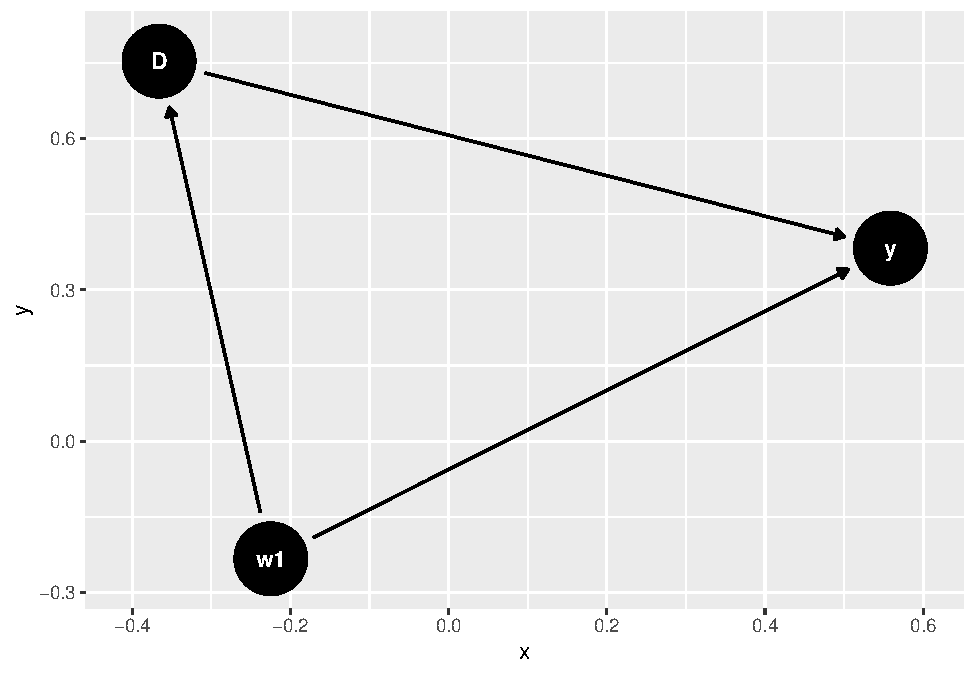
\includegraphics[keepaspectratio]{bookdownproj_files/figure-latex/modelo-mal-especificado-DAG-1.pdf}}

O DAG acima ilustra bem qual a relação causal entre variáveis. Para estimar o ATE de \(D\) sobre \(Y\), precisamos fechar o backdoor de \(w_1\). A forma usual como fazemos isso é com regressão. O problema que estamos abordando aqui é quando a amostra é não-balanceada entre tratados e não-tratados. Vamos visualizar dois tipos de relações (uma linear e outra não-linear) entre a variável de controle \(w_1\) e a resposta \(Y\) para ilustrar o problema do desbalanceamento:

\begin{Shaded}
\begin{Highlighting}[]
\FunctionTok{set.seed}\NormalTok{(}\DecValTok{202}\NormalTok{)}
\NormalTok{n  }\OtherTok{\textless{}{-}} \FloatTok{1e4}
\NormalTok{w1 }\OtherTok{\textless{}{-}} \FunctionTok{rnorm}\NormalTok{(n)                       }\CommentTok{\# único confundidor}
\NormalTok{tau }\OtherTok{\textless{}{-}} \DecValTok{3}                             \CommentTok{\# efeito causal verdadeiro}

\CommentTok{\# GERAMOS UM PROPENSITY SCORE NÃO‐LINEAR}
\NormalTok{p  }\OtherTok{\textless{}{-}} \FunctionTok{plogis}\NormalTok{(}\SpecialCharTok{{-}}\FloatTok{0.5} \SpecialCharTok{+} \DecValTok{2} \SpecialCharTok{*}\NormalTok{ w1) }
\NormalTok{D  }\OtherTok{\textless{}{-}} \FunctionTok{rbinom}\NormalTok{(n, }\DecValTok{1}\NormalTok{, p)}

\CommentTok{\# GERAÇÃO DOS RESULTADOS POTENCIAIS linear (apenas função de w1, forte ignorabilidade):}
\NormalTok{y0 }\OtherTok{\textless{}{-}}  \DecValTok{5} \SpecialCharTok{*}\NormalTok{ w1 }\SpecialCharTok{+} \FunctionTok{rnorm}\NormalTok{(n)}
\NormalTok{y1 }\OtherTok{\textless{}{-}}\NormalTok{ y0 }\SpecialCharTok{{-}}\NormalTok{ tau                       }\CommentTok{\# efeito constante}

\NormalTok{y  }\OtherTok{\textless{}{-}} \FunctionTok{ifelse}\NormalTok{(D }\SpecialCharTok{==} \DecValTok{1}\NormalTok{, y1, y0)}



\NormalTok{df }\OtherTok{\textless{}{-}} \FunctionTok{data.frame}\NormalTok{(}\AttributeTok{y=}\NormalTok{y, }\AttributeTok{D=}\NormalTok{D, }\AttributeTok{w1=}\NormalTok{w1)}

\NormalTok{df }\SpecialCharTok{\%\textgreater{}\%}
  \FunctionTok{mutate}\NormalTok{(}
    \AttributeTok{D =} \FunctionTok{factor}\NormalTok{(D, }\AttributeTok{levels =} \FunctionTok{c}\NormalTok{(}\DecValTok{0}\NormalTok{,}\DecValTok{1}\NormalTok{),}
               \AttributeTok{labels =} \FunctionTok{c}\NormalTok{(}\StringTok{"Controle (D = 0)"}\NormalTok{, }\StringTok{"Tratado (D = 1)"}\NormalTok{))}
\NormalTok{  ) }\SpecialCharTok{\%\textgreater{}\%}
  \FunctionTok{ggplot}\NormalTok{(}\FunctionTok{aes}\NormalTok{(}\AttributeTok{x =}\NormalTok{ w1, }\AttributeTok{y =}\NormalTok{ y, }\AttributeTok{colour =}\NormalTok{ D)) }\SpecialCharTok{+}
  \FunctionTok{geom\_point}\NormalTok{(}\AttributeTok{alpha =} \FloatTok{0.6}\NormalTok{) }\SpecialCharTok{+}
  \FunctionTok{scale\_colour\_manual}\NormalTok{(}
    \AttributeTok{name   =} \StringTok{"Tratamento (binário)"}\NormalTok{,}
    \AttributeTok{values =} \FunctionTok{c}\NormalTok{(}\StringTok{"Controle (D = 0)"} \OtherTok{=} \StringTok{"steelblue"}\NormalTok{, }
               \StringTok{"Tratado (D = 1)"}  \OtherTok{=} \StringTok{"firebrick"}\NormalTok{)}
\NormalTok{  ) }\SpecialCharTok{+} \FunctionTok{theme\_bw}\NormalTok{()}
\end{Highlighting}
\end{Shaded}

\pandocbounded{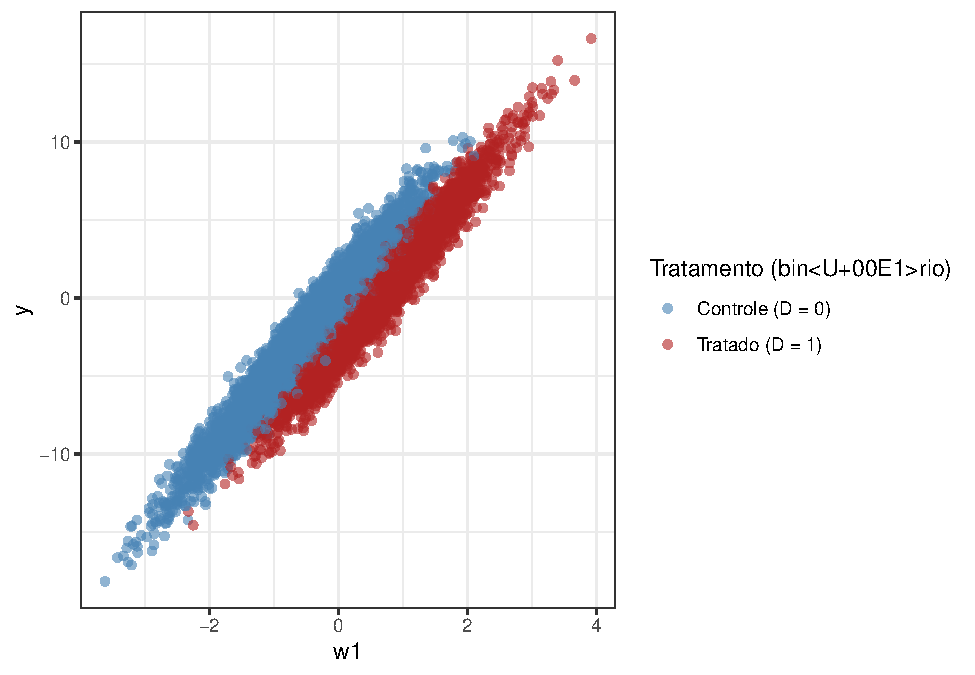
\includegraphics[keepaspectratio]{bookdownproj_files/figure-latex/modelo-mal-especificado-plot1-1.pdf}}

No primeiro gráfico, o efeito causal (ATE) do tratamento é \(-3\) e podemos ver nos dados que de fato em média a resposta é menor entre tratados que no controle. Além disso, vemos também que o efeito é basicamente linear.

Mas o ponto importante aqui é que existem duas regiões dos dados em que praticamente só temos unidades no controle (\(w_1 < -2\)) ou no tratamento (\(w_1 > 2\)). Isso significa que a regressão precisa extrapolar a estimativa da região em que ambos tratamento e controle estão presentes para uma região em que não estão. Como o efeito é constante para todas as regiões de \(w_1\), isso não causa problema e a regressão consegue recuperar o ATE sem viés. O gráfico abaixo ilustra o que a regressão está fazendo:

\begin{Shaded}
\begin{Highlighting}[]
\NormalTok{df }\SpecialCharTok{\%\textgreater{}\%}
  \FunctionTok{mutate}\NormalTok{(}
    \AttributeTok{D =} \FunctionTok{factor}\NormalTok{(D, }\AttributeTok{levels =} \FunctionTok{c}\NormalTok{(}\DecValTok{0}\NormalTok{,}\DecValTok{1}\NormalTok{),}
               \AttributeTok{labels =} \FunctionTok{c}\NormalTok{(}\StringTok{"Controle (D = 0)"}\NormalTok{, }\StringTok{"Tratado (D = 1)"}\NormalTok{))}
\NormalTok{  ) }\SpecialCharTok{\%\textgreater{}\%}
  \FunctionTok{ggplot}\NormalTok{(}\FunctionTok{aes}\NormalTok{(}\AttributeTok{x =}\NormalTok{ w1, }\AttributeTok{y =}\NormalTok{ y, }\AttributeTok{colour =}\NormalTok{ D)) }\SpecialCharTok{+}
  \FunctionTok{geom\_point}\NormalTok{(}\AttributeTok{alpha =} \FloatTok{0.6}\NormalTok{) }\SpecialCharTok{+}
  \FunctionTok{geom\_smooth}\NormalTok{(}\AttributeTok{method =} \StringTok{"lm"}\NormalTok{) }\SpecialCharTok{+}
  \FunctionTok{scale\_colour\_manual}\NormalTok{(}
    \AttributeTok{name   =} \StringTok{"Tratamento (binário)"}\NormalTok{,}
    \AttributeTok{values =} \FunctionTok{c}\NormalTok{(}\StringTok{"Controle (D = 0)"} \OtherTok{=} \StringTok{"steelblue"}\NormalTok{, }
               \StringTok{"Tratado (D = 1)"}  \OtherTok{=} \StringTok{"firebrick"}\NormalTok{)}
\NormalTok{  ) }\SpecialCharTok{+} \FunctionTok{theme\_bw}\NormalTok{()}
\end{Highlighting}
\end{Shaded}

\pandocbounded{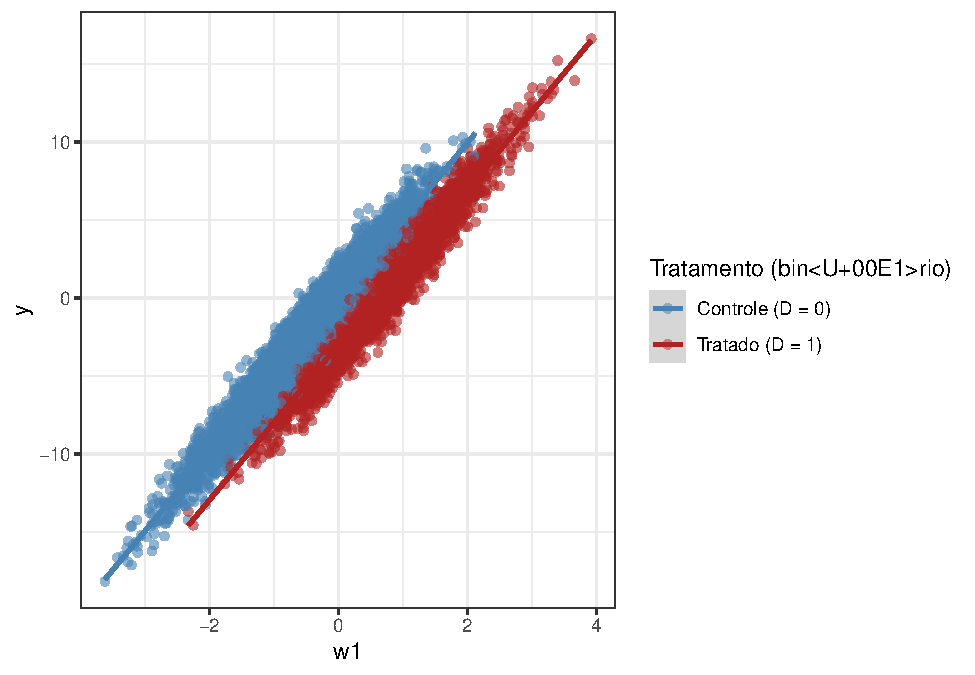
\includegraphics[keepaspectratio]{bookdownproj_files/figure-latex/modelo-mal-especificado-plot1-reg-1.pdf}}

O gráfico mostra duas retas de regressão ajustadas, uma para o controle (em azul) e outra para o tratamento (em vermelho). Efetivamente, temos de estender as duas retas para as regiões em que não há dados, por meio de extrapolação, que no caso significa continuar a linha reta. Assim, temos uma estimativa dos resultados potenciais nessas regiões e podemos computar o efeito causal médio. Como a extrapolação é razoável, não há problema.

Vejamos agora uma situação em que o efeito de \(w_1\) é não linear sobre \(Y\).

\begin{Shaded}
\begin{Highlighting}[]
\FunctionTok{set.seed}\NormalTok{(}\DecValTok{202}\NormalTok{)}
\NormalTok{n  }\OtherTok{\textless{}{-}} \FloatTok{1e4}
\NormalTok{w1 }\OtherTok{\textless{}{-}} \FunctionTok{rnorm}\NormalTok{(n)                       }\CommentTok{\# único confundidor}
\NormalTok{tau }\OtherTok{\textless{}{-}} \DecValTok{3}                             \CommentTok{\# efeito causal verdadeiro}

\CommentTok{\# GERAMOS UM PROPENSITY SCORE NÃO‐LINEAR}
\NormalTok{p  }\OtherTok{\textless{}{-}} \FunctionTok{plogis}\NormalTok{(}\SpecialCharTok{{-}}\FloatTok{0.5} \SpecialCharTok{+} \DecValTok{2} \SpecialCharTok{*}\NormalTok{ w1) }
\NormalTok{D  }\OtherTok{\textless{}{-}} \FunctionTok{rbinom}\NormalTok{(n, }\DecValTok{1}\NormalTok{, p)}

\CommentTok{\# GERAÇÃO DOS RESULTADOS POTENCIAIS não{-}linear (apenas função de w1, forte ignorabilidade):}
\NormalTok{y0 }\OtherTok{\textless{}{-}}  \DecValTok{5} \SpecialCharTok{*}\NormalTok{ w1}\SpecialCharTok{\^{}}\DecValTok{2} \SpecialCharTok{+} \FunctionTok{rnorm}\NormalTok{(n)}
\NormalTok{y1 }\OtherTok{\textless{}{-}}\NormalTok{ y0 }\SpecialCharTok{{-}}\NormalTok{ tau                       }\CommentTok{\# efeito constante}

\NormalTok{y  }\OtherTok{\textless{}{-}} \FunctionTok{ifelse}\NormalTok{(D }\SpecialCharTok{==} \DecValTok{1}\NormalTok{, y1, y0)}



\NormalTok{df }\OtherTok{\textless{}{-}} \FunctionTok{data.frame}\NormalTok{(}\AttributeTok{y=}\NormalTok{y, }\AttributeTok{D=}\NormalTok{D, }\AttributeTok{w1=}\NormalTok{w1)}

\NormalTok{df }\SpecialCharTok{\%\textgreater{}\%}
  \FunctionTok{mutate}\NormalTok{(}
    \AttributeTok{D =} \FunctionTok{factor}\NormalTok{(D, }\AttributeTok{levels =} \FunctionTok{c}\NormalTok{(}\DecValTok{0}\NormalTok{,}\DecValTok{1}\NormalTok{),}
               \AttributeTok{labels =} \FunctionTok{c}\NormalTok{(}\StringTok{"Controle (D = 0)"}\NormalTok{, }\StringTok{"Tratado (D = 1)"}\NormalTok{))}
\NormalTok{  ) }\SpecialCharTok{\%\textgreater{}\%}
  \FunctionTok{ggplot}\NormalTok{(}\FunctionTok{aes}\NormalTok{(}\AttributeTok{x =}\NormalTok{ w1, }\AttributeTok{y =}\NormalTok{ y, }\AttributeTok{colour =}\NormalTok{ D)) }\SpecialCharTok{+}
  \FunctionTok{geom\_point}\NormalTok{(}\AttributeTok{alpha =} \FloatTok{0.6}\NormalTok{) }\SpecialCharTok{+}
  \FunctionTok{scale\_colour\_manual}\NormalTok{(}
    \AttributeTok{name   =} \StringTok{"Tratamento (binário)"}\NormalTok{,}
    \AttributeTok{values =} \FunctionTok{c}\NormalTok{(}\StringTok{"Controle (D = 0)"} \OtherTok{=} \StringTok{"steelblue"}\NormalTok{, }
               \StringTok{"Tratado (D = 1)"}  \OtherTok{=} \StringTok{"firebrick"}\NormalTok{)}
\NormalTok{  ) }\SpecialCharTok{+} \FunctionTok{theme\_bw}\NormalTok{()}
\end{Highlighting}
\end{Shaded}

\pandocbounded{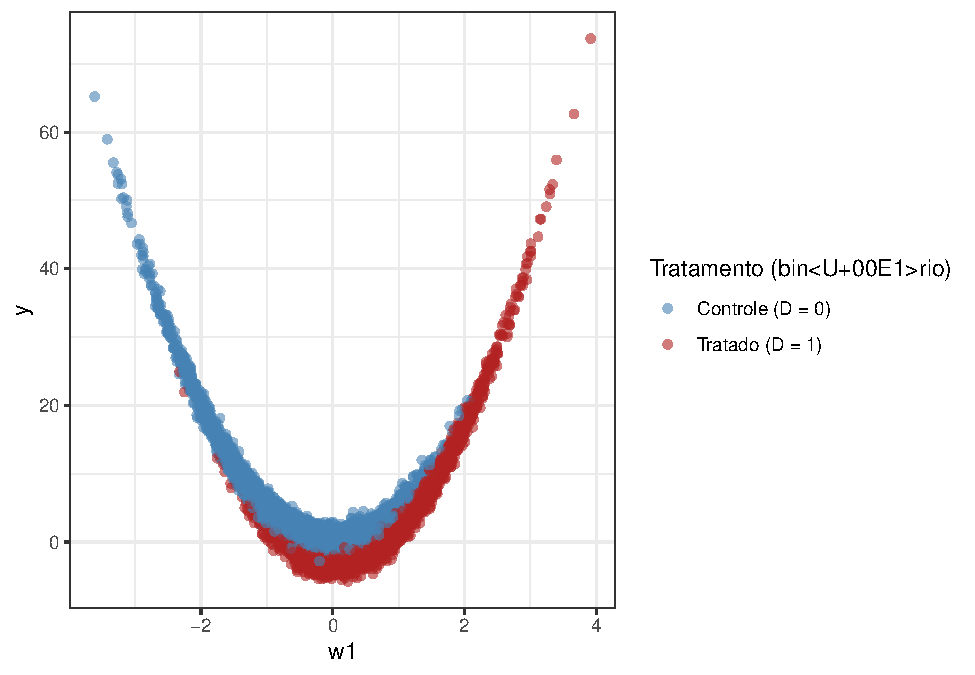
\includegraphics[keepaspectratio]{bookdownproj_files/figure-latex/modelo-mal-especificado-plot2-1.pdf}}

Aqui, vemos que o efeito é não-linear de \(w_1\) sobre \(Y\) e também o desbalanceamento na amostra. Vamos ver o mesmo gráfico com as duas retas ajustadas para entender como a extrapolação pode produzir estimativas distorcidas nesse caso.

\begin{Shaded}
\begin{Highlighting}[]
\NormalTok{df }\SpecialCharTok{\%\textgreater{}\%}
  \FunctionTok{mutate}\NormalTok{(}
    \AttributeTok{D =} \FunctionTok{factor}\NormalTok{(D, }\AttributeTok{levels =} \FunctionTok{c}\NormalTok{(}\DecValTok{0}\NormalTok{,}\DecValTok{1}\NormalTok{),}
               \AttributeTok{labels =} \FunctionTok{c}\NormalTok{(}\StringTok{"Controle (D = 0)"}\NormalTok{, }\StringTok{"Tratado (D = 1)"}\NormalTok{))}
\NormalTok{  ) }\SpecialCharTok{\%\textgreater{}\%}
  \FunctionTok{ggplot}\NormalTok{(}\FunctionTok{aes}\NormalTok{(}\AttributeTok{x =}\NormalTok{ w1, }\AttributeTok{y =}\NormalTok{ y, }\AttributeTok{colour =}\NormalTok{ D)) }\SpecialCharTok{+}
  \FunctionTok{geom\_point}\NormalTok{(}\AttributeTok{alpha =} \FloatTok{0.6}\NormalTok{) }\SpecialCharTok{+}
  \FunctionTok{geom\_smooth}\NormalTok{(}\AttributeTok{method =} \StringTok{"lm"}\NormalTok{) }\SpecialCharTok{+}
  \FunctionTok{scale\_colour\_manual}\NormalTok{(}
    \AttributeTok{name   =} \StringTok{"Tratamento (binário)"}\NormalTok{,}
    \AttributeTok{values =} \FunctionTok{c}\NormalTok{(}\StringTok{"Controle (D = 0)"} \OtherTok{=} \StringTok{"steelblue"}\NormalTok{, }
               \StringTok{"Tratado (D = 1)"}  \OtherTok{=} \StringTok{"firebrick"}\NormalTok{)}
\NormalTok{  ) }\SpecialCharTok{+} \FunctionTok{theme\_bw}\NormalTok{()}
\end{Highlighting}
\end{Shaded}

\pandocbounded{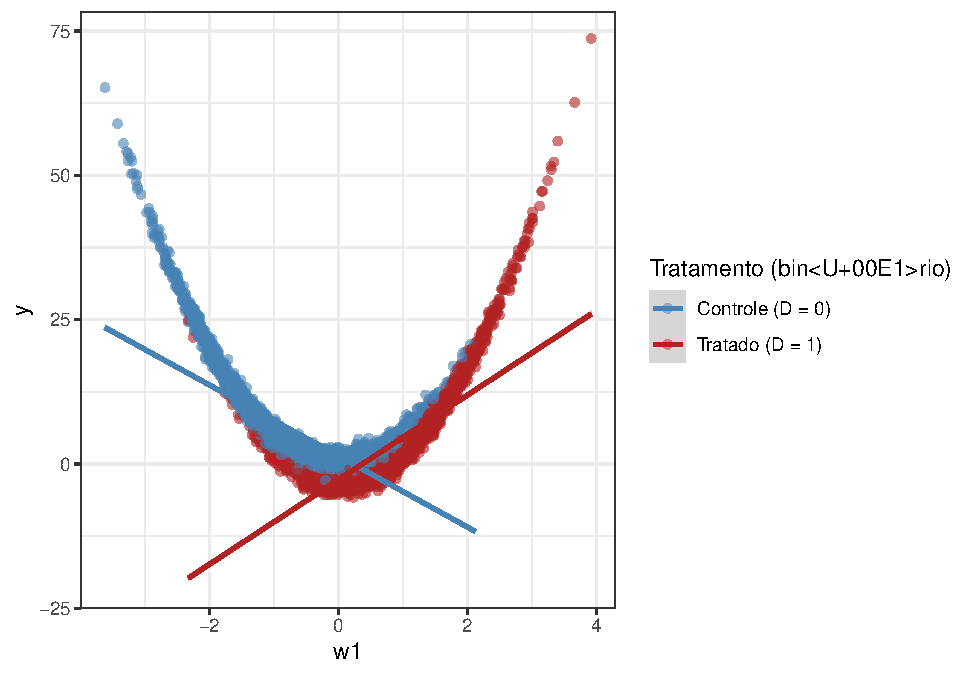
\includegraphics[keepaspectratio]{bookdownproj_files/figure-latex/modelo-mal-especificado-plot2-reg-1.pdf}}

Um problema óbvio do modelo é que o efeito de w1 é quadrático, então podemos tentar corrigir isso incluindo um termo quadrático.

\begin{Shaded}
\begin{Highlighting}[]
\NormalTok{reg\_sq }\OtherTok{\textless{}{-}} \FunctionTok{lm}\NormalTok{(y }\SpecialCharTok{\textasciitilde{}}\NormalTok{ D }\SpecialCharTok{+}\NormalTok{ w1 }\SpecialCharTok{+} \FunctionTok{I}\NormalTok{(w1}\SpecialCharTok{\^{}}\DecValTok{2}\NormalTok{), }\AttributeTok{data =}\NormalTok{ df)}
\FunctionTok{summary}\NormalTok{(reg\_sq)}
\end{Highlighting}
\end{Shaded}

\begin{verbatim}
## 
## Call:
## lm(formula = y ~ D + w1 + I(w1^2), data = df)
## 
## Residuals:
##     Min      1Q  Median      3Q     Max 
## -3.5311 -0.6586 -0.0043  0.6679  3.8928 
## 
## Coefficients:
##              Estimate Std. Error  t value Pr(>|t|)    
## (Intercept) -0.012244   0.015950   -0.768    0.443    
## D           -2.996063   0.025632 -116.890   <2e-16 ***
## w1          -0.013777   0.012639   -1.090    0.276    
## I(w1^2)      5.005598   0.007154  699.737   <2e-16 ***
## ---
## Signif. codes:  0 '***' 0.001 '**' 0.01 '*' 0.05 '.' 0.1 ' ' 1
## 
## Residual standard error: 0.9976 on 9996 degrees of freedom
## Multiple R-squared:  0.9806, Adjusted R-squared:  0.9806 
## F-statistic: 1.688e+05 on 3 and 9996 DF,  p-value: < 2.2e-16
\end{verbatim}

O efeito causal é negativo, o que é bom, pois está na direção certa, mas ainda está distante do efeito verdadeiro. Isso ilustra como a estimativa é dependente do modelo --- um problema sério, pois na prática não sabemos qual é a especificação correta.

Em resumo, quando há desbalanceamento, a estimativa passa a depender fortemente da especificação do modelo, o que é problemático.

Será que existe uma abordagem que nos permita recuperar o efeito causal sem precisar acertar a forma funcional do modelo de outcome? Vamos testar com o propensity score:

\begin{Shaded}
\begin{Highlighting}[]
\NormalTok{reg\_aux}\OtherTok{\textless{}{-}} \FunctionTok{glm}\NormalTok{(D  }\SpecialCharTok{\textasciitilde{}}\NormalTok{ w1, }\AttributeTok{family =}\NormalTok{ binomial, }\AttributeTok{data=}\NormalTok{df)}
\NormalTok{p\_score }\OtherTok{\textless{}{-}}\NormalTok{ reg\_aux}\SpecialCharTok{$}\NormalTok{fitted.values}
\NormalTok{reg1 }\OtherTok{\textless{}{-}} \FunctionTok{lm}\NormalTok{(y }\SpecialCharTok{\textasciitilde{}}\NormalTok{ D }\SpecialCharTok{+}\NormalTok{ p\_score)}
\FunctionTok{summary}\NormalTok{(reg1)}
\end{Highlighting}
\end{Shaded}

\begin{verbatim}
## 
## Call:
## lm(formula = y ~ D + p_score)
## 
## Residuals:
##    Min     1Q Median     3Q    Max 
## -7.921 -4.258 -2.462  1.647 70.708 
## 
## Coefficients:
##             Estimate Std. Error t value Pr(>|t|)    
## (Intercept)   4.2799     0.1179  36.307  < 2e-16 ***
## D            -2.9562     0.1858 -15.910  < 2e-16 ***
## p_score       1.6681     0.2917   5.718 1.11e-08 ***
## ---
## Signif. codes:  0 '***' 0.001 '**' 0.01 '*' 0.05 '.' 0.1 ' ' 1
## 
## Residual standard error: 7.069 on 9997 degrees of freedom
## Multiple R-squared:  0.02781,    Adjusted R-squared:  0.02761 
## F-statistic:   143 on 2 and 9997 DF,  p-value: < 2.2e-16
\end{verbatim}

\begin{Shaded}
\begin{Highlighting}[]
\NormalTok{w }\OtherTok{\textless{}{-}} \FunctionTok{ifelse}\NormalTok{(D }\SpecialCharTok{==} \DecValTok{1}\NormalTok{, }\DecValTok{1}\SpecialCharTok{/}\NormalTok{p\_score, }\DecValTok{1}\SpecialCharTok{/}\NormalTok{(}\DecValTok{1}\SpecialCharTok{{-}}\NormalTok{p\_score))   }\CommentTok{\# pesos IPTW}

\NormalTok{reg2 }\OtherTok{\textless{}{-}} \FunctionTok{lm}\NormalTok{(y }\SpecialCharTok{\textasciitilde{}}\NormalTok{ D , }\AttributeTok{weights =}\NormalTok{ w)}
\FunctionTok{summary}\NormalTok{(reg2)}
\end{Highlighting}
\end{Shaded}

\begin{verbatim}
## 
## Call:
## lm(formula = y ~ D, weights = w)
## 
## Weighted Residuals:
##    Min     1Q Median     3Q    Max 
## -15.95  -5.52  -2.87   2.04 324.89 
## 
## Coefficients:
##             Estimate Std. Error t value Pr(>|t|)    
## (Intercept)  4.67183    0.09553   48.90   <2e-16 ***
## D           -2.57016    0.13452  -19.11   <2e-16 ***
## ---
## Signif. codes:  0 '***' 0.001 '**' 0.01 '*' 0.05 '.' 0.1 ' ' 1
## 
## Residual standard error: 9.499 on 9998 degrees of freedom
## Multiple R-squared:  0.03523,    Adjusted R-squared:  0.03513 
## F-statistic: 365.1 on 1 and 9998 DF,  p-value: < 2.2e-16
\end{verbatim}

Conseguimos recuperar o ATE sem problemas. Não precisei especificar corretamente a forma funcional de \(w_1\) no modelo de outcome, pois o propensity score absorveu a relação entre \(w_1\) e o tratamento. Porém, como discutido acima, o problema de especificação não desapareceu --- ele foi transferido: precisei especificar corretamente o modelo do propensity score (neste caso, um logit linear em \(w_1\), que de fato é o modelo correto do DGP). Se o modelo do PS estivesse errado, o balanceamento falharia --- e isso seria detectável nos diagnósticos.

\subsection{Ponderação por Probabilidade Inversa (IPW)}\label{ponderauxe7uxe3o-por-probabilidade-inversa-ipw}

O código acima já usa uma das aplicações mais importantes do propensity score: a \textbf{ponderação por probabilidade inversa} (IPW, ou IPTW --- \emph{Inverse Probability of Treatment Weighting}). A ideia é reponderar as observações de modo que, na amostra repesada, o tratamento seja independente das covariáveis --- simulando o que um experimento aleatorizado produziria.

O estimador IPW do ATE é:

\[\hat{\tau}_{IPW} = \frac{1}{N}\sum_{i=1}^{N} \left[\frac{D_i Y_i}{\hat{\pi}(X_i)} - \frac{(1-D_i) Y_i}{1-\hat{\pi}(X_i)}\right]\]

A intuição é simples: unidades tratadas com baixa probabilidade de tratamento (baixo \(\hat{\pi}\)) são ``surpreendentes'' --- representam tipos que normalmente não seriam tratados --- e por isso recebem peso maior (\(1/\hat{\pi}\) é grande). O oposto vale para os controles. Essa repesagem reconstrói a distribuição de covariáveis que teríamos sob aleatorização.

Para estimar o ATT em vez do ATE, usamos pesos diferentes: \(w_i = 1\) para os tratados e \(w_i = \hat{\pi}(X_i)/(1-\hat{\pi}(X_i))\) para os controles.

Uma limitação prática do IPW é que, quando o propensity score se aproxima de 0 ou 1 (falta de overlap), os pesos explodem e as estimativas ficam instáveis. Por isso é importante examinar a distribuição do propensity score antes de aplicar IPW, e considerar \emph{trimming} (descartar observações com scores extremos) ou \emph{stabilized weights}.

É útil ver como o pscore está distribuído entre os grupos de tratamento e controle:

\begin{Shaded}
\begin{Highlighting}[]
\NormalTok{df }\OtherTok{\textless{}{-}}\NormalTok{ df }\SpecialCharTok{\%\textgreater{}\%}
  \FunctionTok{mutate}\NormalTok{(}\AttributeTok{pscore =}\NormalTok{ p\_score,}
         \AttributeTok{grupo =} \FunctionTok{factor}\NormalTok{(D, }\AttributeTok{levels =} \FunctionTok{c}\NormalTok{(}\DecValTok{0}\NormalTok{,}\DecValTok{1}\NormalTok{),}
                        \AttributeTok{labels =} \FunctionTok{c}\NormalTok{(}\StringTok{"Controle"}\NormalTok{, }\StringTok{"Tratado"}\NormalTok{)))}

\NormalTok{df }\SpecialCharTok{\%\textgreater{}\%}
  \FunctionTok{ggplot}\NormalTok{(}\FunctionTok{aes}\NormalTok{(}\AttributeTok{x =}\NormalTok{ grupo, }\AttributeTok{y =}\NormalTok{ pscore)) }\SpecialCharTok{+} \FunctionTok{geom\_boxplot}\NormalTok{() }\SpecialCharTok{+}
  \FunctionTok{labs}\NormalTok{(}\AttributeTok{x =} \StringTok{"Grupo"}\NormalTok{, }\AttributeTok{y =} \StringTok{"Propensity Score"}\NormalTok{) }\SpecialCharTok{+} \FunctionTok{theme\_bw}\NormalTok{()}
\end{Highlighting}
\end{Shaded}

\pandocbounded{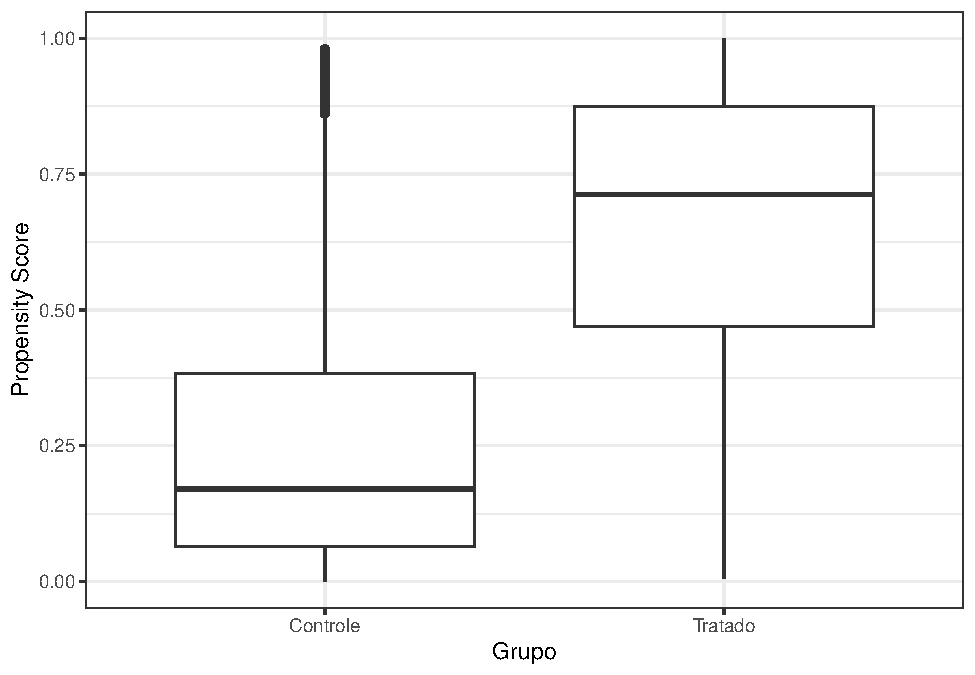
\includegraphics[keepaspectratio]{bookdownproj_files/figure-latex/distribuicao-pscore-1.pdf}}

\begin{Shaded}
\begin{Highlighting}[]
\NormalTok{df }\SpecialCharTok{\%\textgreater{}\%}
  \FunctionTok{ggplot}\NormalTok{(}\FunctionTok{aes}\NormalTok{(}\AttributeTok{x =}\NormalTok{ pscore, }\AttributeTok{colour =}\NormalTok{ grupo)) }\SpecialCharTok{+}
  \FunctionTok{geom\_density}\NormalTok{() }\SpecialCharTok{+}
  \FunctionTok{labs}\NormalTok{(}\AttributeTok{x =} \StringTok{"Propensity Score"}\NormalTok{, }\AttributeTok{y =} \StringTok{"Densidade"}\NormalTok{, }\AttributeTok{colour =} \StringTok{"Grupo"}\NormalTok{) }\SpecialCharTok{+} \FunctionTok{theme\_bw}\NormalTok{()}
\end{Highlighting}
\end{Shaded}

\pandocbounded{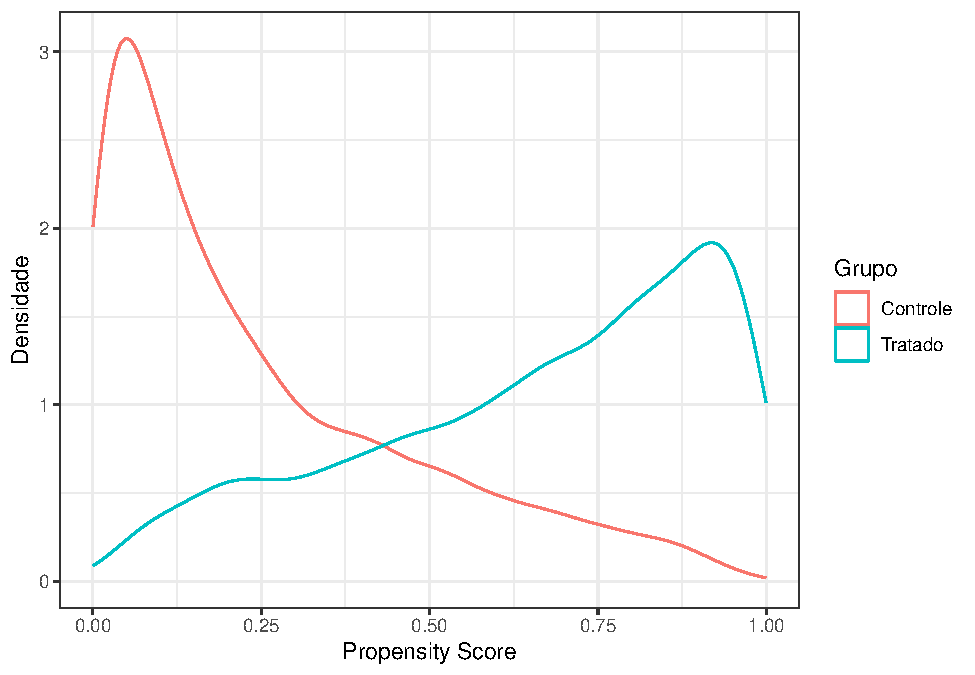
\includegraphics[keepaspectratio]{bookdownproj_files/figure-latex/distribuicao-pscore-2.pdf}}

Há desbalanceamento e falta de overlap ou suporte comum, o que leva à extrapolação.

\subsection{Matching}\label{matching}

\subsubsection{Intuição}\label{intuiuxe7uxe3o}

A ideia do matching pode ser ilustrada se notarmos o seguinte. A projeção da reta vermelha para pontos abaixo de \(-2\) é de um \(y\) médio muito baixo, enquanto que o \(y\) médio é muito alto para o controle. O oposto é verificado para a região em que \(w_1 > 2\). Portanto, se restringirmos a análise para uma região onde há overlap entre tratados e controles, a necessidade de extrapolação diminui. O que acontece com a estimativa? Vamos comparar a regressão com toda a amostra e com subconjuntos cada vez mais restritos:

\begin{Shaded}
\begin{Highlighting}[]
\NormalTok{reg\_sub }\OtherTok{\textless{}{-}} \FunctionTok{lm}\NormalTok{(y }\SpecialCharTok{\textasciitilde{}}\NormalTok{ D }\SpecialCharTok{+}\NormalTok{ w1, }\AttributeTok{data =}\NormalTok{ df)}

\NormalTok{reg\_sub }\SpecialCharTok{\%\textgreater{}\%}
  \FunctionTok{tidy}\NormalTok{() }\SpecialCharTok{\%\textgreater{}\%}
  \FunctionTok{kable}\NormalTok{(}\AttributeTok{digits =} \FunctionTok{c}\NormalTok{(}\DecValTok{0}\NormalTok{, }\DecValTok{2}\NormalTok{, }\DecValTok{3}\NormalTok{, }\DecValTok{2}\NormalTok{, }\DecValTok{3}\NormalTok{))}
\end{Highlighting}
\end{Shaded}

\begin{tabular}{l|r|r|r|r}
\hline
term & estimate & std.error & statistic & p.value\\
\hline
(Intercept) & 4.27 & 0.104 & 41.00 & 0\\
\hline
D & -1.30 & 0.180 & -7.18 & 0\\
\hline
w1 & -0.80 & 0.089 & -8.94 & 0\\
\hline
\end{tabular}

\begin{Shaded}
\begin{Highlighting}[]
\NormalTok{reg\_sub }\OtherTok{\textless{}{-}} \FunctionTok{lm}\NormalTok{(y }\SpecialCharTok{\textasciitilde{}}\NormalTok{ D }\SpecialCharTok{+}\NormalTok{ w1, }\AttributeTok{data =} \FunctionTok{subset}\NormalTok{(df, w1 }\SpecialCharTok{\textgreater{}} \SpecialCharTok{{-}}\DecValTok{2} \SpecialCharTok{\&}\NormalTok{ w1 }\SpecialCharTok{\textless{}} \DecValTok{2}\NormalTok{))}

\NormalTok{reg\_sub }\SpecialCharTok{\%\textgreater{}\%}
  \FunctionTok{tidy}\NormalTok{() }\SpecialCharTok{\%\textgreater{}\%}
  \FunctionTok{kable}\NormalTok{(}\AttributeTok{digits =} \FunctionTok{c}\NormalTok{(}\DecValTok{0}\NormalTok{, }\DecValTok{2}\NormalTok{, }\DecValTok{3}\NormalTok{, }\DecValTok{2}\NormalTok{, }\DecValTok{3}\NormalTok{))}
\end{Highlighting}
\end{Shaded}

\begin{tabular}{l|r|r|r|r}
\hline
term & estimate & std.error & statistic & p.value\\
\hline
(Intercept) & 3.46 & 0.069 & 50.52 & 0\\
\hline
D & -1.99 & 0.119 & -16.70 & 0\\
\hline
w1 & -0.35 & 0.066 & -5.32 & 0\\
\hline
\end{tabular}

\begin{Shaded}
\begin{Highlighting}[]
\NormalTok{reg\_sub }\OtherTok{\textless{}{-}} \FunctionTok{lm}\NormalTok{(y }\SpecialCharTok{\textasciitilde{}}\NormalTok{ D }\SpecialCharTok{+}\NormalTok{ w1, }\AttributeTok{data =} \FunctionTok{subset}\NormalTok{(df, w1 }\SpecialCharTok{\textgreater{}} \SpecialCharTok{{-}}\FloatTok{1.5} \SpecialCharTok{\&}\NormalTok{ w1 }\SpecialCharTok{\textless{}} \FloatTok{1.5}\NormalTok{))}

\NormalTok{reg\_sub }\SpecialCharTok{\%\textgreater{}\%}
  \FunctionTok{tidy}\NormalTok{() }\SpecialCharTok{\%\textgreater{}\%}
  \FunctionTok{kable}\NormalTok{(}\AttributeTok{digits =} \FunctionTok{c}\NormalTok{(}\DecValTok{0}\NormalTok{, }\DecValTok{2}\NormalTok{, }\DecValTok{3}\NormalTok{, }\DecValTok{2}\NormalTok{, }\DecValTok{3}\NormalTok{))}
\end{Highlighting}
\end{Shaded}

\begin{tabular}{l|r|r|r|r}
\hline
term & estimate & std.error & statistic & p.value\\
\hline
(Intercept) & 2.57 & 0.047 & 55.02 & 0\\
\hline
D & -2.48 & 0.080 & -30.78 & 0\\
\hline
w1 & -0.21 & 0.053 & -3.88 & 0\\
\hline
\end{tabular}

\begin{Shaded}
\begin{Highlighting}[]
\NormalTok{reg\_sub }\OtherTok{\textless{}{-}} \FunctionTok{lm}\NormalTok{(y }\SpecialCharTok{\textasciitilde{}}\NormalTok{ D }\SpecialCharTok{+}\NormalTok{ w1, }\AttributeTok{data =} \FunctionTok{subset}\NormalTok{(df, w1 }\SpecialCharTok{\textgreater{}} \SpecialCharTok{{-}}\DecValTok{1} \SpecialCharTok{\&}\NormalTok{ w1 }\SpecialCharTok{\textless{}} \DecValTok{1}\NormalTok{))}

\NormalTok{reg\_sub }\SpecialCharTok{\%\textgreater{}\%}
  \FunctionTok{tidy}\NormalTok{() }\SpecialCharTok{\%\textgreater{}\%}
  \FunctionTok{kable}\NormalTok{(}\AttributeTok{digits =} \FunctionTok{c}\NormalTok{(}\DecValTok{0}\NormalTok{, }\DecValTok{2}\NormalTok{, }\DecValTok{3}\NormalTok{, }\DecValTok{2}\NormalTok{, }\DecValTok{3}\NormalTok{))}
\end{Highlighting}
\end{Shaded}

\begin{tabular}{l|r|r|r|r}
\hline
term & estimate & std.error & statistic & p.value\\
\hline
(Intercept) & 1.41 & 0.029 & 49.57 & 0\\
\hline
D & -2.77 & 0.048 & -57.27 & 0\\
\hline
w1 & -0.17 & 0.043 & -3.93 & 0\\
\hline
\end{tabular}

À medida que restringimos a amostra para regiões com mais overlap, a estimativa se aproxima do efeito causal verdadeiro (\(-3\)). Isso confirma que o problema estava na extrapolação, não na regressão em si.

A ideia do matching é um pouco diferente do que fizemos acima, pois estamos excluindo as observações que estão no tratamento e que não possuem controle correspondente, e do controle que não possuem tratamento correspondente. Não há erro em excluir os dois tipos de observações, mas sempre temos de nos perguntar qual é o estimando de interesse. Se faço esse procedimento, o meu estimando não é nenhum dos usuais ATT ou ATE.

No matching, nós nos concentramos em estimar o ATT, de forma que procuramos achar observações no controle que são próximas das tratadas, ou seja, excluímos os controles que não são um match para as observações tratadas.

\subsubsection{Matching como imputação}\label{matching-como-imputauxe7uxe3o}

A técnica de matching trata os resultados potenciais como \emph{missing data}. Assim, se pudermos supor CIA com credibilidade, pelo menos com relação a \(Y_i(0)\), então podemos imputar esses resultados potenciais e estimar o ATT. A ideia é achar uma unidade o mais similar possível à unidade tratada para servir como contrafactual. Assim, poderíamos computar ``diretamente'' o ATT, já que teríamos os \(Y_i(1)\) e \(Y_i(0)\) para cada unidade, este último imputado.

Há dois grandes grupos de métodos de matching: exato e aproximado. Note que o matching, por construção, é um procedimento assimétrico: pegamos cada unidade tratada e buscamos o controle mais parecido. Todos os tratados são usados, mas controles sem match são descartados. Esse procedimento pondera implicitamente pela distribuição de \(X\) nos tratados --- e portanto estima o \textbf{ATT}, não o ATE. Na população com \(n \to \infty\) e propensity score verdadeiro, tanto o ATE quanto o ATT são identificados (pois o suporte comum é satisfeito para todos os valores de \(X\)). Mas o estimador de matching como implementado na prática --- buscar controle para cada tratado --- estima o ATT. Quem quiser o ATE deve usar IPW, AIPW ou full matching.

\subsubsection{Matching exato}\label{matching-exato}

Uma vez que temos as suposições de identificação, podemos discutir os métodos para realizar o matching. O mais simples deles é o matching exato. Nesse método, nós achamos uma unidade (ou mais) que tenham um valor exatamente igual nas covariáveis (ou no propensity score), e imputamos o controle.

\subsubsection{Matching aproximado}\label{matching-aproximado}

Para aproximar o matching, utilizamos alguma noção de distância entre variáveis. Para mais de uma variável, podemos utilizar algumas métricas de distância. A primeira é a distância euclidiana (supondo \(K\) variáveis).

\[
\lVert X_i - X_j \rVert = \sqrt{(X_i - X_j)'(X_i - X_j)} = \sqrt{\sum_{k=1}^K(X_{ki} - X_{kj})^2}
\]

A distância euclidiana utiliza a escala das proprias variaveis, então é comum usar a distância euclidiana normalizada:

\[
\lVert X_i - X_j \rVert = \sqrt{\sum_{k=1}^K\frac{(X_{ki} - X_{kj})^2}{\hat{\sigma}_k^2}}
\]

Outra métrica é a distância de Mahalanobis, que basicamente divide pela covariância (amostral) entre as variáveis em vez da variância. Na prática, a distância euclidiana normalizada é a mais comum.

\subsubsection{Estimando}\label{estimando-1}

Uma vez que fizemos o matching entre unidades, qual nosso estimador? Lembrando que o estimando é o ATT. Denotando por \(N_T = \sum_{i=1}^N D_i\) o número de unidades tratadas e por \(j(i)\) o índice da unidade de controle que é o match da unidade tratada \(i\), temos:
\[
\widehat{\delta}_{ATT} = \dfrac{1}{N_T} \sum_{D_i=1} (Y_i - Y_{j(i)})
\]

\begin{Shaded}
\begin{Highlighting}[]
\NormalTok{result\_0 }\OtherTok{\textless{}{-}} \FunctionTok{matchit}\NormalTok{(D }\SpecialCharTok{\textasciitilde{}}\NormalTok{ w1, }\AttributeTok{data =}\NormalTok{ df, }\AttributeTok{method =} \ConstantTok{NULL}\NormalTok{, }\AttributeTok{distance =} \StringTok{\textquotesingle{}glm\textquotesingle{}}\NormalTok{)}
\FunctionTok{summary}\NormalTok{(result\_0)}
\end{Highlighting}
\end{Shaded}

\begin{verbatim}
## 
## Call:
## matchit(formula = D ~ w1, data = df, method = NULL, distance = "glm")
## 
## Summary of Balance for All Data:
##          Means Treated Means Control Std. Mean Diff. Var. Ratio eCDF Mean
## distance        0.6549        0.2493          1.5714     1.2566    0.3685
## w1              0.7004       -0.5362          1.6030     0.9132    0.3685
##          eCDF Max
## distance   0.5761
## w1         0.5761
## 
## Sample Sizes:
##           Control Treated
## All          5806    4194
## Matched      5806    4194
## Unmatched       0       0
## Discarded       0       0
\end{verbatim}

\subsection{Aplicação: o dataset LaLonde}\label{aplicauxe7uxe3o-o-dataset-lalonde}

O dataset LaLonde é um dos exemplos mais influentes na literatura de inferência causal. O pesquisador Lalonde (\citeproc{ref-lalonde1986}{1986}) investigou se métodos econométricos tradicionais eram capazes de recuperar o efeito causal de um programa experimental --- o National Supported Work Demonstration (NSW), que oferecia emprego temporário para dar experiência de trabalho. Ele coletou dados de um survey representativo de trabalhadores americanos (PSID) e usou esses trabalhadores como grupo controle, empregando diversos métodos econométricos para estimar o efeito causal. Os resultados foram desastrosos: altamente variáveis dependendo do modelo e subconjunto de dados, frequentemente com sinal errado.

Vamos replicar esse exercício usando matching e propensity score. A variável resposta é \texttt{re78} (renda real em 1978), o tratamento é \texttt{treat}, e as demais variáveis são covariáveis.

\begin{Shaded}
\begin{Highlighting}[]
\FunctionTok{set.seed}\NormalTok{(}\DecValTok{1234}\NormalTok{)}
\end{Highlighting}
\end{Shaded}

\begin{Shaded}
\begin{Highlighting}[]
\NormalTok{lalonde }\OtherTok{\textless{}{-}} \FunctionTok{fread}\NormalTok{(}\FunctionTok{here}\NormalTok{(}\StringTok{"Dados"}\NormalTok{, }\StringTok{"lalonde\_nsw.csv"}\NormalTok{))}
\NormalTok{psid\_data }\OtherTok{\textless{}{-}} \FunctionTok{fread}\NormalTok{(}\FunctionTok{here}\NormalTok{(}\StringTok{"Dados"}\NormalTok{, }\StringTok{"lalonde\_psid.csv"}\NormalTok{))}

\CommentTok{\# Combinamos tratados do NSW com controles do PSID}
\NormalTok{nsw\_treat }\OtherTok{\textless{}{-}}\NormalTok{ lalonde[lalonde}\SpecialCharTok{$}\NormalTok{treat }\SpecialCharTok{==} \DecValTok{1}\NormalTok{, ]}
\NormalTok{psid\_control }\OtherTok{\textless{}{-}}\NormalTok{ psid\_data[psid\_data}\SpecialCharTok{$}\NormalTok{treat }\SpecialCharTok{==} \DecValTok{0}\NormalTok{, ]}
\NormalTok{dw\_data }\OtherTok{\textless{}{-}} \FunctionTok{rbind}\NormalTok{(nsw\_treat, psid\_control)}
\end{Highlighting}
\end{Shaded}

\subsubsection{Diferença bruta}\label{diferenuxe7a-bruta}

A diferença simples na média entre tratados e controles não é causal, pois os grupos diferem sistematicamente nas covariáveis. Note o resultado --- a diferença bruta é negativa, sugerindo que o programa \emph{reduziu} a renda dos participantes. Mas sabemos, pela estimativa experimental, que o efeito verdadeiro é positivo (aproximadamente \$1.794). O viés de seleção inverte completamente o sinal. Será que matching e propensity score conseguem corrigir isso?

\begin{Shaded}
\begin{Highlighting}[]
\NormalTok{dw\_data }\SpecialCharTok{\%\textgreater{}\%}
    \FunctionTok{group\_by}\NormalTok{(treat) }\SpecialCharTok{\%\textgreater{}\%}
    \FunctionTok{summarize}\NormalTok{(}\StringTok{\textasciigrave{}}\AttributeTok{Renda média (1978)}\StringTok{\textasciigrave{}} \OtherTok{=} \FunctionTok{mean}\NormalTok{(re78)) }\SpecialCharTok{\%\textgreater{}\%}
\NormalTok{    kableExtra}\SpecialCharTok{::}\FunctionTok{kable}\NormalTok{(}\AttributeTok{digits =} \DecValTok{0}\NormalTok{, }\AttributeTok{col.names =} \FunctionTok{c}\NormalTok{(}\StringTok{"Tratamento"}\NormalTok{, }\StringTok{"Renda média (1978)"}\NormalTok{))}
\end{Highlighting}
\end{Shaded}

\begin{verbatim}
## Warning in do.call(data.frame, c(x, alis)): unable to translate 'Renda
## m<U+00E9>dia (1978)' to native encoding
\end{verbatim}

\begin{tabular}{r|r}
\hline
Tratamento & Renda m<U+00E9>dia (1978)\\
\hline
0 & 21554\\
\hline
1 & 6349\\
\hline
\end{tabular}

\subsubsection{Balanceamento pré-matching}\label{balanceamento-pruxe9-matching}

Antes de fazer matching, examinamos o desbalanceamento nas covariáveis. O \texttt{matchit} com \texttt{method\ =\ NULL} calcula o propensity score e as medidas de balanceamento sem realizar matching:

\begin{Shaded}
\begin{Highlighting}[]
\NormalTok{m.out0 }\OtherTok{\textless{}{-}} \FunctionTok{matchit}\NormalTok{(treat }\SpecialCharTok{\textasciitilde{}}\NormalTok{ age }\SpecialCharTok{+}\NormalTok{ education }\SpecialCharTok{+}\NormalTok{ hispanic }\SpecialCharTok{+}\NormalTok{ black }\SpecialCharTok{+}\NormalTok{ married }\SpecialCharTok{+}\NormalTok{ nodegree }\SpecialCharTok{+}\NormalTok{ re74 }\SpecialCharTok{+}\NormalTok{ re75,}
                  \AttributeTok{data =}\NormalTok{ dw\_data,}
                  \AttributeTok{method =} \ConstantTok{NULL}\NormalTok{,}
                  \AttributeTok{distance =} \StringTok{"glm"}\NormalTok{)}
\end{Highlighting}
\end{Shaded}

\begin{verbatim}
## Warning: glm.fit: fitted probabilities numerically 0 or 1 occurred
\end{verbatim}

\begin{Shaded}
\begin{Highlighting}[]
\FunctionTok{summary}\NormalTok{(m.out0)}
\end{Highlighting}
\end{Shaded}

\begin{verbatim}
## 
## Call:
## matchit(formula = treat ~ age + education + hispanic + black + 
##     married + nodegree + re74 + re75, data = dw_data, method = NULL, 
##     distance = "glm")
## 
## Summary of Balance for All Data:
##           Means Treated Means Control Std. Mean Diff. Var. Ratio eCDF Mean
## distance         0.6364        0.0270          2.1674     8.0268    0.4816
## age             25.8162       34.8506         -1.2627     0.4696    0.2317
## education       10.3459       12.1169         -0.8808     0.4255    0.1091
## hispanic         0.0595        0.0325          0.1139          .    0.0269
## black            0.8432        0.2506          1.6301          .    0.5926
## married          0.1892        0.8663         -1.7287          .    0.6771
## nodegree         0.7081        0.3052          0.8862          .    0.4029
## re74          2095.5737    19428.7458         -3.5471     0.1329    0.4684
## re75          1532.0553    19063.3377         -5.4458     0.0561    0.4695
##           eCDF Max
## distance    0.8817
## age         0.3771
## education   0.4029
## hispanic    0.0269
## black       0.5926
## married     0.6771
## nodegree    0.4029
## re74        0.7292
## re75        0.7736
## 
## Sample Sizes:
##           Control Treated
## All          2490     185
## Matched      2490     185
## Unmatched       0       0
## Discarded       0       0
\end{verbatim}

O desbalanceamento é severo, especialmente em \texttt{black}, \texttt{re74} e \texttt{re75} --- exatamente as variáveis que Lalonde (\citeproc{ref-lalonde1986}{1986}) identificou como problemáticas. Vamos agora aplicar matching para tentar corrigir isso.

\subsubsection{Nearest-neighbor matching}\label{nearest-neighbor-matching}

Começamos com o matching por vizinho mais próximo (\emph{nearest-neighbor}) no propensity score:

\begin{Shaded}
\begin{Highlighting}[]
\NormalTok{m.out1 }\OtherTok{\textless{}{-}} \FunctionTok{matchit}\NormalTok{(treat }\SpecialCharTok{\textasciitilde{}}\NormalTok{ age }\SpecialCharTok{+}\NormalTok{ education }\SpecialCharTok{+}\NormalTok{ hispanic }\SpecialCharTok{+}\NormalTok{ black }\SpecialCharTok{+}\NormalTok{ married }\SpecialCharTok{+}\NormalTok{ nodegree }\SpecialCharTok{+}\NormalTok{ re74 }\SpecialCharTok{+}\NormalTok{ re75,}
                  \AttributeTok{data =}\NormalTok{ dw\_data,}
                  \AttributeTok{method =} \StringTok{"nearest"}\NormalTok{,}
                  \AttributeTok{distance =} \StringTok{"glm"}\NormalTok{)}
\end{Highlighting}
\end{Shaded}

\begin{verbatim}
## Warning: glm.fit: fitted probabilities numerically 0 or 1 occurred
\end{verbatim}

\begin{Shaded}
\begin{Highlighting}[]
\FunctionTok{summary}\NormalTok{(m.out1)}
\end{Highlighting}
\end{Shaded}

\begin{verbatim}
## 
## Call:
## matchit(formula = treat ~ age + education + hispanic + black + 
##     married + nodegree + re74 + re75, data = dw_data, method = "nearest", 
##     distance = "glm")
## 
## Summary of Balance for All Data:
##           Means Treated Means Control Std. Mean Diff. Var. Ratio eCDF Mean
## distance         0.6364        0.0270          2.1674     8.0268    0.4816
## age             25.8162       34.8506         -1.2627     0.4696    0.2317
## education       10.3459       12.1169         -0.8808     0.4255    0.1091
## hispanic         0.0595        0.0325          0.1139          .    0.0269
## black            0.8432        0.2506          1.6301          .    0.5926
## married          0.1892        0.8663         -1.7287          .    0.6771
## nodegree         0.7081        0.3052          0.8862          .    0.4029
## re74          2095.5737    19428.7458         -3.5471     0.1329    0.4684
## re75          1532.0553    19063.3377         -5.4458     0.0561    0.4695
##           eCDF Max
## distance    0.8817
## age         0.3771
## education   0.4029
## hispanic    0.0269
## black       0.5926
## married     0.6771
## nodegree    0.4029
## re74        0.7292
## re75        0.7736
## 
## Summary of Balance for Matched Data:
##           Means Treated Means Control Std. Mean Diff. Var. Ratio eCDF Mean
## distance         0.6364        0.2934          1.2200     1.4702    0.0432
## age             25.8162       30.4811         -0.6520     0.4149    0.1196
## education       10.3459       10.3784         -0.0161     0.4745    0.0407
## hispanic         0.0595        0.0649         -0.0229          .    0.0054
## black            0.8432        0.7568          0.2379          .    0.0865
## married          0.1892        0.4595         -0.6901          .    0.2703
## nodegree         0.7081        0.6216          0.1902          .    0.0865
## re74          2095.5737     4499.8428         -0.4920     1.1020    0.0722
## re75          1532.0553     3204.3968         -0.5195     0.7389    0.0605
##           eCDF Max Std. Pair Dist.
## distance    0.5568          1.2200
## age         0.1784          1.3561
## education   0.0919          1.3281
## hispanic    0.0054          0.5257
## black       0.0865          0.9515
## married     0.2703          1.0213
## nodegree    0.0865          0.9036
## re74        0.4162          0.8667
## re75        0.2973          0.9044
## 
## Sample Sizes:
##           Control Treated
## All          2490     185
## Matched       185     185
## Unmatched    2305       0
## Discarded       0       0
\end{verbatim}

\begin{Shaded}
\begin{Highlighting}[]
\FunctionTok{plot}\NormalTok{(}\FunctionTok{summary}\NormalTok{(m.out1))}
\end{Highlighting}
\end{Shaded}

\pandocbounded{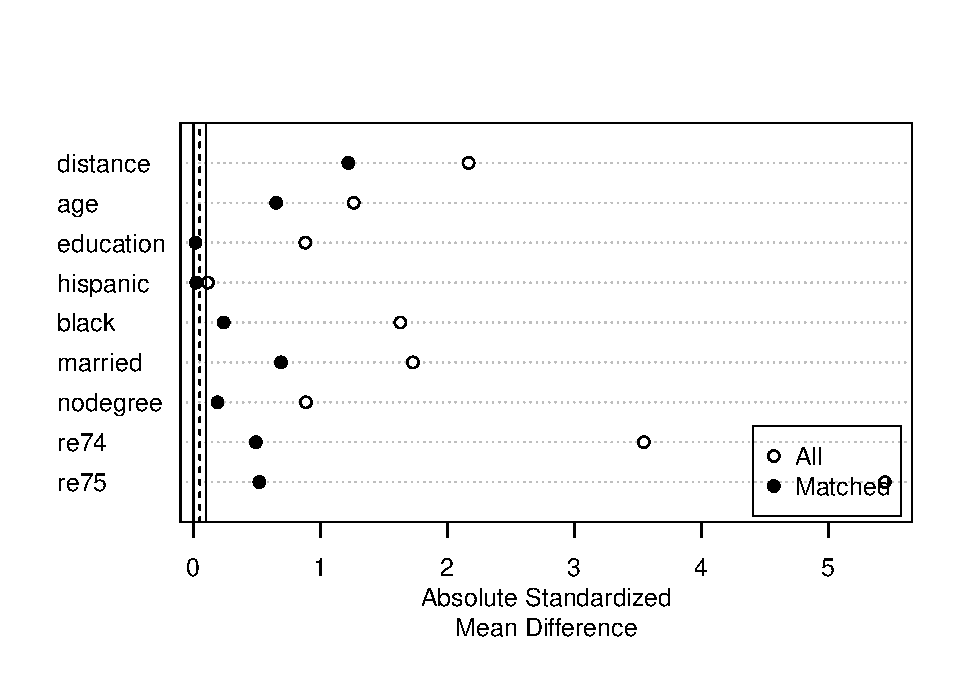
\includegraphics[keepaspectratio]{bookdownproj_files/figure-latex/matching-nearest-1.pdf}}

O gráfico de \emph{love plot} mostra as diferenças padronizadas antes e depois do matching. Idealmente, todas as covariáveis deveriam ter diferenças próximas de zero após o matching.

\subsubsection{Full matching}\label{full-matching}

Uma alternativa é o \emph{full matching}, que usa todas as observações (sem descarte) e cria subclasses de tamanho variável:

\begin{Shaded}
\begin{Highlighting}[]
\NormalTok{m.out2 }\OtherTok{\textless{}{-}} \FunctionTok{matchit}\NormalTok{(treat }\SpecialCharTok{\textasciitilde{}}\NormalTok{ age }\SpecialCharTok{+}\NormalTok{ education }\SpecialCharTok{+}\NormalTok{ hispanic }\SpecialCharTok{+}\NormalTok{ black }\SpecialCharTok{+}\NormalTok{ married }\SpecialCharTok{+}\NormalTok{ nodegree }\SpecialCharTok{+}\NormalTok{ re74 }\SpecialCharTok{+}\NormalTok{ re75,}
                  \AttributeTok{data =}\NormalTok{ dw\_data,}
                  \AttributeTok{method =} \StringTok{"full"}\NormalTok{,}
                  \AttributeTok{distance =} \StringTok{"glm"}\NormalTok{)}
\end{Highlighting}
\end{Shaded}

\begin{verbatim}
## Warning: glm.fit: fitted probabilities numerically 0 or 1 occurred
\end{verbatim}

\begin{Shaded}
\begin{Highlighting}[]
\FunctionTok{summary}\NormalTok{(m.out2)}
\end{Highlighting}
\end{Shaded}

\begin{verbatim}
## 
## Call:
## matchit(formula = treat ~ age + education + hispanic + black + 
##     married + nodegree + re74 + re75, data = dw_data, method = "full", 
##     distance = "glm")
## 
## Summary of Balance for All Data:
##           Means Treated Means Control Std. Mean Diff. Var. Ratio eCDF Mean
## distance         0.6364        0.0270          2.1674     8.0268    0.4816
## age             25.8162       34.8506         -1.2627     0.4696    0.2317
## education       10.3459       12.1169         -0.8808     0.4255    0.1091
## hispanic         0.0595        0.0325          0.1139          .    0.0269
## black            0.8432        0.2506          1.6301          .    0.5926
## married          0.1892        0.8663         -1.7287          .    0.6771
## nodegree         0.7081        0.3052          0.8862          .    0.4029
## re74          2095.5737    19428.7458         -3.5471     0.1329    0.4684
## re75          1532.0553    19063.3377         -5.4458     0.0561    0.4695
##           eCDF Max
## distance    0.8817
## age         0.3771
## education   0.4029
## hispanic    0.0269
## black       0.5926
## married     0.6771
## nodegree    0.4029
## re74        0.7292
## re75        0.7736
## 
## Summary of Balance for Matched Data:
##           Means Treated Means Control Std. Mean Diff. Var. Ratio eCDF Mean
## distance         0.6364        0.6338          0.0091     0.9750    0.0034
## age             25.8162       23.5784          0.3128     0.9777    0.0779
## education       10.3459       10.1846          0.0802     0.6511    0.0258
## hispanic         0.0595        0.0722         -0.0537          .    0.0127
## black            0.8432        0.8485         -0.0144          .    0.0052
## married          0.1892        0.1337          0.1417          .    0.0555
## nodegree         0.7081        0.7121         -0.0087          .    0.0040
## re74          2095.5737     3369.8141         -0.2608     1.4024    0.0443
## re75          1532.0553     2341.0260         -0.2513     0.7348    0.0299
##           eCDF Max Std. Pair Dist.
## distance    0.1243          0.0059
## age         0.2923          1.2717
## education   0.1181          1.3984
## hispanic    0.0127          0.1697
## black       0.0052          1.9737
## married     0.0555          0.3408
## nodegree    0.0040          1.3976
## re74        0.5207          2.2676
## re75        0.2243          1.9077
## 
## Sample Sizes:
##               Control Treated
## All           2490.       185
## Matched (ESS)   23.03     185
## Matched       2490.       185
## Unmatched        0.         0
## Discarded        0.         0
\end{verbatim}

\subsubsection{Estimação do ATT}\label{estimauxe7uxe3o-do-att}

Com o matching feito, estimamos o ATT usando regressão com interações nas covariáveis (para ajuste residual) e erros-padrão clusterizados por subclasse:

\begin{Shaded}
\begin{Highlighting}[]
\CommentTok{\# Com nearest{-}neighbor}
\NormalTok{m.data1 }\OtherTok{\textless{}{-}} \FunctionTok{match.data}\NormalTok{(m.out1)}
\NormalTok{fit1 }\OtherTok{\textless{}{-}} \FunctionTok{lm}\NormalTok{(re78 }\SpecialCharTok{\textasciitilde{}}\NormalTok{ treat }\SpecialCharTok{*}\NormalTok{ (age }\SpecialCharTok{+}\NormalTok{ education }\SpecialCharTok{+}\NormalTok{ hispanic }\SpecialCharTok{+}\NormalTok{ black }\SpecialCharTok{+}\NormalTok{ married }\SpecialCharTok{+}
\NormalTok{                             nodegree }\SpecialCharTok{+}\NormalTok{ re74 }\SpecialCharTok{+}\NormalTok{ re75),}
           \AttributeTok{data =}\NormalTok{ m.data1, }\AttributeTok{weights =}\NormalTok{ weights)}

\FunctionTok{avg\_comparisons}\NormalTok{(fit1, }\AttributeTok{variables =} \StringTok{"treat"}\NormalTok{,}
                \AttributeTok{vcov =} \SpecialCharTok{\textasciitilde{}}\NormalTok{subclass, }\AttributeTok{newdata =} \FunctionTok{subset}\NormalTok{(treat }\SpecialCharTok{==} \DecValTok{1}\NormalTok{))}
\end{Highlighting}
\end{Shaded}

\begin{verbatim}
## 
##  Estimate Std. Error    z Pr(>|z|)   S 2.5 % 97.5 %
##      1905        872 2.18    0.029 5.1   195   3614
## 
## Term: treat
## Type:  response 
## Comparison: 1 - 0
\end{verbatim}

\begin{Shaded}
\begin{Highlighting}[]
\CommentTok{\# Com full matching}
\NormalTok{m.data2 }\OtherTok{\textless{}{-}} \FunctionTok{match.data}\NormalTok{(m.out2)}
\NormalTok{fit2 }\OtherTok{\textless{}{-}} \FunctionTok{lm}\NormalTok{(re78 }\SpecialCharTok{\textasciitilde{}}\NormalTok{ treat }\SpecialCharTok{*}\NormalTok{ (age }\SpecialCharTok{+}\NormalTok{ education }\SpecialCharTok{+}\NormalTok{ hispanic }\SpecialCharTok{+}\NormalTok{ black }\SpecialCharTok{+}\NormalTok{ married }\SpecialCharTok{+}
\NormalTok{                             nodegree }\SpecialCharTok{+}\NormalTok{ re74 }\SpecialCharTok{+}\NormalTok{ re75),}
           \AttributeTok{data =}\NormalTok{ m.data2, }\AttributeTok{weights =}\NormalTok{ weights)}

\FunctionTok{avg\_comparisons}\NormalTok{(fit2, }\AttributeTok{variables =} \StringTok{"treat"}\NormalTok{,}
                \AttributeTok{vcov =} \SpecialCharTok{\textasciitilde{}}\NormalTok{subclass, }\AttributeTok{newdata =} \FunctionTok{subset}\NormalTok{(treat }\SpecialCharTok{==} \DecValTok{1}\NormalTok{))}
\end{Highlighting}
\end{Shaded}

\begin{verbatim}
## 
##  Estimate Std. Error    z Pr(>|z|)    S 2.5 % 97.5 %
##      2629        612 4.29   <0.001 15.8  1429   3829
## 
## Term: treat
## Type:  response 
## Comparison: 1 - 0
\end{verbatim}

A estimativa experimental do NSW é de aproximadamente \$1.794. Compare as estimativas do nearest-neighbor e do full matching com essa referência. Qual método chegou mais perto? Por quê? Note que nenhuma das estimativas é \emph{exatamente} igual ao benchmark --- isso ilustra que matching com dados observacionais é uma aproximação, não uma garantia.

\subsection{Recomendações Práticas sobre Matching}\label{recomendauxe7uxf5es-pruxe1ticas-sobre-matching}

Rotina ou algoritmo:

\begin{enumerate}
\def\labelenumi{\arabic{enumi}.}
\item
  Defina o que é proximidade: alguma distância de medida para determinar se um caso é um bom match e quais variáveis utilizar. Em geral, distância euclidiana.
\item
  Implemente o método do match.
\item
  Avalie a qualidade do método, por meio do balanceamento antes e depois do match. Se necessário, altere o passo 1 ou 2 e itere.
\item
  Faça a inferência sobre o efeito causal do tratamento sobre a resposta, dado o matching feito em 3.
\end{enumerate}

\subsubsection{Avaliação do matching feito}\label{avaliauxe7uxe3o-do-matching-feito}

\begin{enumerate}
\def\labelenumi{\arabic{enumi}.}
\item
  É melhor usar matching exato ou aproximado do que propensity score matching (cf. \citeproc{ref-kingnielsen2019}{King and Nielsen 2019}). O argumento é o seguinte: o propensity score é um escalar que resume todas as covariáveis. Duas unidades podem ter o mesmo \(\hat{\pi}(X)\) mas perfis de covariáveis completamente diferentes --- por exemplo, um jovem com alta educação e um idoso com baixa educação podem ter a mesma probabilidade estimada de tratamento. Quando se faz matching por propensity score, é possível que o balanceamento nas covariáveis individuais \textbf{piore} à medida que os pares ficam mais próximos no score --- o que King and Nielsen (\citeproc{ref-kingnielsen2019}{2019}) chamam de \emph{propensity score paradox}. Isso aumenta a dependência do modelo de outcome, exatamente o que matching deveria evitar.

  É importante notar que esse problema é de \textbf{amostra finita}: na população, o teorema de Rosenbaum-Rubin garante que condicionar no propensity score verdadeiro \(\pi(X)\) produz balanceamento perfeito em todas as covariáveis (pois \(D \perp X | \pi(X)\)). Com infinitas observações para cada valor do score, a média sobre todas as unidades com \(\pi(X) = c\) produz balanceamento exato. O paradoxo surge porque, na amostra, o score é estimado (não verdadeiro), o número de unidades com score similar é pequeno, e o matching seleciona \emph{um} controle em vez de promediar sobre todos.

  Métodos que trabalham diretamente no espaço das covariáveis --- como CEM, Mahalanobis, ou entropy balancing --- monitoram diretamente o balanceamento em vez de delegá-lo a um escalar estimado. Note que a crítica se aplica ao propensity score como \textbf{métrica de distância para matching}, não a outros usos: IPW (ponderação), subclassificação e estimadores duplamente robustos (AIPW) continuam válidos.
\item
  Não devemos fazer teste de hipótese para checar que o balanceamento após matching é melhor do que antes (amostra menor reduz o poder do teste de detectar desbalanceamento. Além disso, não há superpopulação alvo da inferência, pois balanceamento é uma propriedade de uma amostra em particular) (cf. \citeproc{ref-austin2009}{Austin 2009}).
\item
  Além de comparar médias, é recomendado comparar variâncias ou desvios-padrão (\citeproc{ref-austin2009}{Austin 2009}). Por exemplo, razão de variâncias.
\item
  Jamais use a variável resposta para fazer o matching.
\item
  Matching com reposição gera dificuldades para calcular o erro padrão, já que a mesma unidade de controle pode servir de match para múltiplos tratados, criando dependência entre as observações. Abadie e Imbens (2006) mostram que o bootstrap ingênuo é \textbf{inconsistente} para o erro padrão do estimador de nearest-neighbor matching --- ou seja, não converge para o valor correto mesmo com \(n \to \infty\). O pacote \texttt{MatchIt} em R lida com isso ao recomendar o uso de erros-padrão clusterizados por subclasse (\texttt{vcov\ =\ \textasciitilde{}subclass}) na análise pós-matching.
\end{enumerate}

\subsection{Métodos modernos de matching}\label{muxe9todos-modernos-de-matching}

\subsubsection{Coarsened Exact Matching (CEM)}\label{coarsened-exact-matching-cem}

O Coarsened Exact Matching (CEM, \citeproc{ref-iacuskingporro2012}{Iacus, King, and Porro 2012}) é um método que busca combinar a simplicidade do matching exato com a flexibilidade do matching aproximado. A ideia é ``engrossar'' (\emph{coarsen}) temporariamente as covariáveis --- por exemplo, agrupar idades em faixas etárias (18--25, 26--35, etc.) --- e então realizar matching exato nas versões engrossadas. As observações que não encontram match exato nas covariáveis engrossadas são descartadas. Após o matching, a análise é feita com os valores originais (não engrossados) das covariáveis.

A vantagem principal do CEM é que ele garante um nível máximo de desbalanceamento ex ante: o pesquisador escolhe o grau de engrossamento e, portanto, controla diretamente o trade-off entre qualidade do match e tamanho da amostra resultante. Além disso, o CEM satisfaz uma propriedade chamada \emph{monotonic imbalance bounding}: engrossar menos (faixas mais estreitas) nunca piora o balanceamento.

\begin{Shaded}
\begin{Highlighting}[]
\NormalTok{m.cem }\OtherTok{\textless{}{-}} \FunctionTok{matchit}\NormalTok{(treat }\SpecialCharTok{\textasciitilde{}}\NormalTok{ age }\SpecialCharTok{+}\NormalTok{ education }\SpecialCharTok{+}\NormalTok{ hispanic }\SpecialCharTok{+}\NormalTok{ black }\SpecialCharTok{+}\NormalTok{ married }\SpecialCharTok{+}\NormalTok{ nodegree }\SpecialCharTok{+}\NormalTok{ re74 }\SpecialCharTok{+}\NormalTok{ re75,}
                 \AttributeTok{data =}\NormalTok{ dw\_data, }\AttributeTok{method =} \StringTok{"cem"}\NormalTok{)}
\FunctionTok{summary}\NormalTok{(m.cem)}
\end{Highlighting}
\end{Shaded}

\begin{verbatim}
## 
## Call:
## matchit(formula = treat ~ age + education + hispanic + black + 
##     married + nodegree + re74 + re75, data = dw_data, method = "cem")
## 
## Summary of Balance for All Data:
##           Means Treated Means Control Std. Mean Diff. Var. Ratio eCDF Mean
## age             25.8162       34.8506         -1.2627     0.4696    0.2317
## education       10.3459       12.1169         -0.8808     0.4255    0.1091
## hispanic         0.0595        0.0325          0.1139          .    0.0269
## black            0.8432        0.2506          1.6301          .    0.5926
## married          0.1892        0.8663         -1.7287          .    0.6771
## nodegree         0.7081        0.3052          0.8862          .    0.4029
## re74          2095.5737    19428.7458         -3.5471     0.1329    0.4684
## re75          1532.0553    19063.3377         -5.4458     0.0561    0.4695
##           eCDF Max
## age         0.3771
## education   0.4029
## hispanic    0.0269
## black       0.5926
## married     0.6771
## nodegree    0.4029
## re74        0.7292
## re75        0.7736
## 
## Summary of Balance for Matched Data:
##           Means Treated Means Control Std. Mean Diff. Var. Ratio eCDF Mean
## age             24.9569       24.9639         -0.0010     1.0568    0.0082
## education       10.5259       10.5057          0.0100     1.0467    0.0027
## hispanic         0.0086        0.0086          0.0000          .    0.0000
## black            0.8966        0.8966         -0.0000          .    0.0000
## married          0.2500        0.2500         -0.0000          .    0.0000
## nodegree         0.6724        0.6724         -0.0000          .    0.0000
## re74          1852.5830     5084.9418         -0.6615     0.9346    0.0911
## re75          1314.5073     4929.6785         -1.1230     0.4560    0.1246
##           eCDF Max Std. Pair Dist.
## age         0.0991          0.1257
## education   0.0187          0.1059
## hispanic    0.0000          0.0000
## black       0.0000          0.0000
## married     0.0000          0.0000
## nodegree    0.0000          0.0000
## re74        0.5774          0.7826
## re75        0.5595          1.3340
## 
## Sample Sizes:
##               Control Treated
## All           2490.       185
## Matched (ESS)   50.79     116
## Matched        131.       116
## Unmatched     2359.        69
## Discarded        0.         0
\end{verbatim}

\begin{Shaded}
\begin{Highlighting}[]
\NormalTok{m.data.cem }\OtherTok{\textless{}{-}} \FunctionTok{match.data}\NormalTok{(m.cem)}
\NormalTok{fit.cem }\OtherTok{\textless{}{-}} \FunctionTok{lm}\NormalTok{(re78 }\SpecialCharTok{\textasciitilde{}}\NormalTok{ treat }\SpecialCharTok{*}\NormalTok{ (age }\SpecialCharTok{+}\NormalTok{ education }\SpecialCharTok{+}\NormalTok{ black }\SpecialCharTok{+}\NormalTok{ married }\SpecialCharTok{+}
\NormalTok{                                nodegree }\SpecialCharTok{+}\NormalTok{ re74 }\SpecialCharTok{+}\NormalTok{ re75),}
              \AttributeTok{data =}\NormalTok{ m.data.cem, }\AttributeTok{weights =}\NormalTok{ weights)}

\FunctionTok{avg\_comparisons}\NormalTok{(fit.cem, }\AttributeTok{variables =} \StringTok{"treat"}\NormalTok{,}
                \AttributeTok{vcov =} \SpecialCharTok{\textasciitilde{}}\NormalTok{subclass, }\AttributeTok{newdata =} \FunctionTok{subset}\NormalTok{(treat }\SpecialCharTok{==} \DecValTok{1}\NormalTok{))}
\end{Highlighting}
\end{Shaded}

\begin{verbatim}
## 
##  Estimate Std. Error     z Pr(>|z|)   S 2.5 % 97.5 %
##       316       1460 0.216    0.829 0.3 -2546   3178
## 
## Term: treat
## Type:  response 
## Comparison: 1 - 0
\end{verbatim}

Note o trade-off: o CEM descarta observações que não encontram match exato nas covariáveis engrossadas. Compare o número de observações usadas com o nearest-neighbor matching.

\subsubsection{Entropy Balancing}\label{entropy-balancing}

O entropy balancing (\citeproc{ref-hainmueller2012}{Hainmueller 2012}) adota uma abordagem diferente: em vez de selecionar observações, ele repesa as unidades do grupo de controle de modo que momentos selecionados (média, variância e, opcionalmente, assimetria) das covariáveis no controle repesado sejam exatamente iguais aos do grupo tratado. Isso é feito resolvendo um problema de otimização convexa que minimiza a entropia dos pesos em relação a pesos uniformes, sujeito às restrições de balanceamento.

Na prática, o entropy balancing produz pesos suaves (sem descarte de observações) e garante balanceamento exato nos momentos especificados, eliminando a necessidade de iterar entre matching e checagem de balanceamento. É uma alternativa atraente quando o número de covariáveis é moderado e o pesquisador quer evitar a perda de observações associada ao matching tradicional.

\begin{Shaded}
\begin{Highlighting}[]
\FunctionTok{library}\NormalTok{(ebal)}

\CommentTok{\# Separar tratados e controles}
\NormalTok{treated }\OtherTok{\textless{}{-}}\NormalTok{ dw\_data[dw\_data}\SpecialCharTok{$}\NormalTok{treat }\SpecialCharTok{==} \DecValTok{1}\NormalTok{, ]}
\NormalTok{control }\OtherTok{\textless{}{-}}\NormalTok{ dw\_data[dw\_data}\SpecialCharTok{$}\NormalTok{treat }\SpecialCharTok{==} \DecValTok{0}\NormalTok{, ]}

\NormalTok{covs }\OtherTok{\textless{}{-}} \FunctionTok{c}\NormalTok{(}\StringTok{"age"}\NormalTok{, }\StringTok{"education"}\NormalTok{, }\StringTok{"hispanic"}\NormalTok{, }\StringTok{"black"}\NormalTok{, }\StringTok{"married"}\NormalTok{, }\StringTok{"nodegree"}\NormalTok{, }\StringTok{"re74"}\NormalTok{, }\StringTok{"re75"}\NormalTok{)}

\NormalTok{eb }\OtherTok{\textless{}{-}} \FunctionTok{ebalance}\NormalTok{(}\AttributeTok{Treatment =}\NormalTok{ dw\_data}\SpecialCharTok{$}\NormalTok{treat,}
               \AttributeTok{X =}\NormalTok{ dw\_data[, ..covs])}

\CommentTok{\# Médias das covariáveis: tratados vs controles repesados}
\FunctionTok{round}\NormalTok{(eb}\SpecialCharTok{$}\NormalTok{co.xdata, }\DecValTok{3}\NormalTok{)}
\end{Highlighting}
\end{Shaded}

\begin{verbatim}
##           age education hispanic black married nodegree       re74       re75
##    [1,] 1  47        12        0     0       0        0      0.000      0.000
##    [2,] 1  50        12        0     1       1        0      0.000      0.000
##    [3,] 1  44        12        0     0       0        0      0.000      0.000
##    [4,] 1  28        12        0     1       1        0      0.000      0.000
##    [5,] 1  54        12        0     0       1        0      0.000      0.000
##    [6,] 1  55        12        1     0       1        0      0.000      0.000
##    [7,] 1  47        12        0     0       1        0      0.000      0.000
##    [8,] 1  25        12        0     1       0        0      0.000      0.000
##    [9,] 1  44        12        0     0       1        0      0.000      0.000
##   [10,] 1  50        12        0     1       1        0      0.000      0.000
##   [11,] 1  23        12        0     1       0        0      0.000      0.000
##   [12,] 1  49        14        0     0       1        0      0.000      0.000
##   [13,] 1  55        14        0     0       1        0      0.000      0.000
##   [14,] 1  34        14        0     1       1        0      0.000      0.000
##   [15,] 1  34        16        0     0       1        0      0.000      0.000
##   [16,] 1  55        13        1     0       1        0      0.000      0.000
##   [17,] 1  52        12        0     0       1        0      0.000      0.000
##   [18,] 1  52        15        0     0       1        0      0.000      0.000
##   [19,] 1  30        16        0     0       1        0      0.000      0.000
##   [20,] 1  21        12        0     0       0        0      0.000      0.000
##   [21,] 1  30        17        0     0       0        0      0.000      0.000
##   [22,] 1  44        12        0     0       1        0      0.000      0.000
##   [23,] 1  46        12        0     0       0        0      0.000      0.000
##   [24,] 1  53        17        0     0       1        0      0.000      0.000
##   [25,] 1  26        16        0     0       0        0      0.000      0.000
##   [26,] 1  49        12        0     0       1        0      0.000      0.000
##   [27,] 1  39        15        0     0       1        0      0.000      0.000
##   [28,] 1  26        17        0     0       1        0      0.000      0.000
##   [29,] 1  32        16        0     0       1        0      0.000      0.000
##   [30,] 1  34        12        0     0       1        0      0.000      0.000
##   [31,] 1  31        14        0     0       1        0      0.000      0.000
##   [32,] 1  39        17        1     0       1        0      0.000      0.000
##   [33,] 1  40        17        0     0       1        0      0.000      0.000
##   [34,] 1  31        12        0     0       1        0      0.000      0.000
##   [35,] 1  27        13        0     0       1        0      0.000      0.000
##   [36,] 1  48        12        0     0       1        0      0.000      0.000
##   [37,] 1  41        13        0     0       1        0      0.000      0.000
##   [38,] 1  26        14        0     0       0        0      0.000      0.000
##   [39,] 1  50        17        0     0       0        0      0.000      0.000
##   [40,] 1  48        12        0     0       1        0      0.000      0.000
##   [41,] 1  45        16        0     0       1        0      0.000      0.000
##   [42,] 1  37        13        0     0       1        0      0.000      0.000
##   [43,] 1  33        12        0     0       1        0      0.000      0.000
##   [44,] 1  31        12        0     0       1        0      0.000      0.000
##   [45,] 1  36        12        0     1       1        0      0.000      0.000
##   [46,] 1  44        13        0     0       1        0      0.000      0.000
##   [47,] 1  28        17        0     0       1        0      0.000      0.000
##   [48,] 1  30        17        0     0       1        0      0.000      0.000
##   [49,] 1  42        16        0     0       1        0      0.000      0.000
##   [50,] 1  30        12        0     0       1        0      0.000      0.000
##   [51,] 1  27        16        0     0       1        0      0.000      0.000
##   [52,] 1  37        12        0     0       1        0      0.000      0.000
##   [53,] 1  37        12        0     0       1        0      0.000      0.000
##   [54,] 1  45        12        0     0       1        0      0.000      0.000
##   [55,] 1  35        16        0     0       1        0      0.000      0.000
##   [56,] 1  37        17        0     0       1        0      0.000      0.000
##   [57,] 1  27        17        0     0       1        0      0.000      0.000
##   [58,] 1  47        14        0     0       1        0      0.000      0.000
##   [59,] 1  48        12        0     0       1        0      0.000      0.000
##   [60,] 1  42        12        0     0       1        0      0.000      0.000
##   [61,] 1  43        12        0     0       1        0      0.000      0.000
##   [62,] 1  46        12        0     0       1        0      0.000      0.000
##   [63,] 1  46        12        0     0       1        0      0.000      0.000
##   [64,] 1  46        12        0     0       1        0      0.000      0.000
##   [65,] 1  29        16        0     0       1        0      0.000      0.000
##   [66,] 1  39        13        0     0       1        0      0.000      0.000
##   [67,] 1  32        12        0     0       1        0      0.000      0.000
##   [68,] 1  48        16        0     0       1        0      0.000      0.000
##   [69,] 1  48        16        0     0       1        0      0.000      0.000
##   [70,] 1  41        13        0     0       1        0      0.000      0.000
##   [71,] 1  42        13        0     0       1        0      0.000      0.000
##   [72,] 1  42        13        0     0       1        0      0.000      0.000
##   [73,] 1  42        13        0     0       1        0      0.000      0.000
##   [74,] 1  54        13        0     0       1        0      0.000      0.000
##   [75,] 1  29        14        0     0       1        0      0.000      0.000
##   [76,] 1  54        12        0     0       1        0      0.000      0.000
##   [77,] 1  54        12        0     0       1        0      0.000      0.000
##   [78,] 1  26        14        0     0       1        0      0.000      0.000
##   [79,] 1  43        17        0     0       1        0      0.000      0.000
##   [80,] 1  54        12        0     0       1        0      0.000      0.000
##   [81,] 1  37        12        0     0       1        0      0.000      0.000
##   [82,] 1  54        16        0     0       1        0      0.000      0.000
##   [83,] 1  48        17        0     0       1        0      0.000      0.000
##   [84,] 1  44        12        0     0       1        0      0.000      0.000
##   [85,] 1  54        12        0     0       1        0      0.000      0.000
##   [86,] 1  38        12        0     0       1        0      0.000      0.000
##   [87,] 1  37        13        0     0       1        0      0.000      0.000
##   [88,] 1  27        17        0     0       1        0      0.000      0.000
##   [89,] 1  51        12        0     0       1        0      0.000      0.000
##   [90,] 1  39        12        0     0       1        0      0.000      0.000
##   [91,] 1  55        14        0     0       1        0      0.000      0.000
##   [92,] 1  54        13        0     0       1        0      0.000      0.000
##   [93,] 1  54        13        0     0       1        0      0.000      0.000
##   [94,] 1  34        12        0     0       1        0      0.000      0.000
##   [95,] 1  50        14        0     0       1        0      0.000      0.000
##   [96,] 1  50        12        0     0       1        0      0.000      0.000
##   [97,] 1  21        14        1     0       0        0      0.000     71.613
##   [98,] 1  26        12        0     0       1        0      0.000     71.613
##   [99,] 1  21        13        0     0       0        0      0.000    692.855
##  [100,] 1  23        16        0     0       1        0      0.000   1521.774
##  [101,] 1  21        15        0     0       0        0      0.000   3222.581
##  [102,] 1  23        14        0     0       0        0      0.000   3401.613
##  [103,] 1  27        16        0     0       1        0      0.000   4833.871
##  [104,] 1  25        12        0     0       1        0      0.000   5729.032
##  [105,] 1  27        17        0     0       0        0      0.000   6087.097
##  [106,] 1  55        12        0     0       1        0      0.000   6266.129
##  [107,] 1  20        12        0     0       1        0      0.000   7161.291
##  [108,] 1  18        12        0     0       1        0      0.000   8056.452
##  [109,] 1  27        12        0     0       1        0      0.000   8235.484
##  [110,] 1  28        16        0     0       1        0      0.000   8951.613
##  [111,] 1  36        12        0     1       1        0      0.000   8951.613
##  [112,] 1  33        13        0     1       1        0      0.000  10741.935
##  [113,] 1  36        12        0     0       1        0      0.000  10741.935
##  [114,] 1  27        13        0     0       1        0      0.000  16112.903
##  [115,] 1  45        17        0     0       1        0      0.000  16112.903
##  [116,] 1  45        17        0     0       1        0      0.000  16112.903
##  [117,] 1  45        17        0     0       1        0      0.000  16112.903
##  [118,] 1  31        12        0     0       1        0      0.000  17903.227
##  [119,] 1  34        12        0     0       1        0      0.000  17903.227
##  [120,] 1  34        12        0     0       1        0      0.000  17903.227
##  [121,] 1  47        14        0     0       1        0      0.000  17903.227
##  [122,] 1  35        16        0     0       1        0      0.000  19693.549
##  [123,] 1  43        17        0     0       1        0      0.000  21161.613
##  [124,] 1  25        12        0     1       1        0      0.000  21483.871
##  [125,] 1  29        15        0     0       0        0      0.000  21483.871
##  [126,] 1  31        12        0     0       1        0      0.000  21483.871
##  [127,] 1  52        12        0     0       1        0      0.000  21483.871
##  [128,] 1  22        16        0     0       0        0      0.000  22558.064
##  [129,] 1  53        15        0     0       1        0      0.000  24169.355
##  [130,] 1  29        17        0     0       1        0      0.000  25959.678
##  [131,] 1  31        13        0     0       1        0      0.000  25959.678
##  [132,] 1  35        12        0     0       1        0      0.000  26138.711
##  [133,] 1  29        16        0     0       1        0      0.000  26854.840
##  [134,] 1  39        12        0     0       1        0      0.000  28645.160
##  [135,] 1  37        14        0     0       1        0      0.000  32225.807
##  [136,] 1  30        14        0     0       1        0      0.000  32225.807
##  [137,] 1  43        17        0     0       1        0      0.000  42251.613
##  [138,] 1  32        17        0     0       1        0      0.000  46548.387
##  [139,] 1  44        12        0     0       1        0      0.000  71612.906
##  [140,] 1  32        16        0     0       1        0    577.984   6910.645
##  [141,] 1  43        12        0     1       1        0    715.132   1879.839
##  [142,] 1  24        12        0     1       0        0    783.707      0.000
##  [143,] 1  22        13        0     0       0        0    783.707      0.000
##  [144,] 1  35        15        0     0       1        0    979.633    537.097
##  [145,] 1  26        15        0     0       0        0    979.633   1879.839
##  [146,] 1  29        17        0     0       1        0    979.633   8951.613
##  [147,] 1  23        12        0     1       0        0   1077.597   3222.581
##  [148,] 1  19        12        0     0       1        0   1154.008   8593.549
##  [149,] 1  48        16        0     0       1        0   1240.216   1466.274
##  [150,] 1  48        16        0     0       1        0   1240.216   1466.274
##  [151,] 1  22        12        0     1       1        0   1269.605      0.000
##  [152,] 1  20        12        0     1       0        0   1367.568  12532.258
##  [153,] 1  24        17        0     0       1        0   1371.487      0.000
##  [154,] 1  27        16        0     0       1        0   1469.450   1253.226
##  [155,] 1  21        14        0     0       0        0   1506.676   2685.484
##  [156,] 1  53        13        0     0       1        0   1567.413   3938.710
##  [157,] 1  53        13        0     0       1        0   1567.413   3938.710
##  [158,] 1  53        16        0     0       1        0   1665.377      0.000
##  [159,] 1  22        15        0     0       1        0   1763.340   5370.968
##  [160,] 1  21        15        0     0       0        0   1763.340   9667.742
##  [161,] 1  30        12        0     0       1        0   1959.267   1790.323
##  [162,] 1  21        12        0     1       0        0   1959.267   5460.484
##  [163,] 1  27        16        0     0       1        0   1959.267  17545.160
##  [164,] 1  22        15        0     0       0        0   1967.104   2864.516
##  [165,] 1  22        12        0     1       1        0   2006.289   2470.645
##  [166,] 1  23        13        0     0       1        0   2155.194   5370.968
##  [167,] 1  33        12        0     0       1        0   2351.120      0.000
##  [168,] 1  24        13        0     0       0        0   2351.120   3127.694
##  [169,] 1  20        12        0     1       0        0   2351.120   4475.807
##  [170,] 1  22        16        0     0       0        0   2351.120  23274.193
##  [171,] 1  19        12        0     0       1        0   2547.047  10741.935
##  [172,] 1  22        15        0     0       1        0   2547.047  17187.098
##  [173,] 1  43        14        0     0       1        0   2645.010      0.000
##  [174,] 1  39        12        0     0       1        0   2742.973   7161.291
##  [175,] 1  28        12        0     1       0        0   2938.900   2864.516
##  [176,] 1  19        14        0     0       0        0   2938.900   3222.581
##  [177,] 1  26        17        0     0       1        0   2938.900  12532.258
##  [178,] 1  18        12        0     0       1        0   3134.827  11100.000
##  [179,] 1  23        15        0     0       1        0   3320.957   2506.452
##  [180,] 1  24        12        0     1       0        0   3330.754   4654.839
##  [181,] 1  27        12        0     0       1        0   3526.680      0.000
##  [182,] 1  29        17        0     0       1        0   3526.680  15217.742
##  [183,] 1  22        12        0     1       0        0   3579.580  17133.387
##  [184,] 1  27        12        0     0       1        0   3722.607    254.226
##  [185,] 1  27        15        0     0       1        0   3722.607   4654.839
##  [186,] 1  20        12        0     1       0        0   3730.444   8951.613
##  [187,] 1  27        12        0     1       1        0   3918.534   1994.419
##  [188,] 1  23        12        0     1       1        0   3918.534   2864.516
##  [189,] 1  23        12        0     1       1        0   3918.534  11637.097
##  [190,] 1  22        12        0     0       1        0   3918.534  15396.774
##  [191,] 1  31        12        0     1       1        0   3918.534  18440.322
##  [192,] 1  26        17        0     0       0        0   4173.238  11637.097
##  [193,] 1  20        12        0     0       1        0   4310.387      0.000
##  [194,] 1  30        17        0     0       1        0   4310.387   4296.774
##  [195,] 1  42        16        0     0       0        0   4398.554  17903.227
##  [196,] 1  21        14        0     0       1        0   4506.313   9309.678
##  [197,] 1  25        16        0     0       1        0   4604.277   2954.032
##  [198,] 1  27        15        0     0       1        0   4702.240      0.000
##  [199,] 1  26        17        0     0       1        0   4702.240  19693.549
##  [200,] 1  29        16        0     0       1        0   4800.204  17187.098
##  [201,] 1  20        12        0     0       0        0   4811.959    716.129
##  [202,] 1  52        12        0     0       1        0   4898.167      0.000
##  [203,] 1  23        17        0     0       0        0   4898.167   2148.387
##  [204,] 1  21        14        0     0       1        0   4898.167   7161.291
##  [205,] 1  24        16        0     0       0        0   4898.167   8951.613
##  [206,] 1  30        17        0     0       1        0   4898.167  12084.677
##  [207,] 1  25        17        0     0       0        0   4996.130  17414.469
##  [208,] 1  21        12        0     0       1        0   5094.094   6803.226
##  [209,] 1  28        12        0     0       1        0   5094.094  10741.935
##  [210,] 1  20        12        0     0       1        0   5182.261   6266.129
##  [211,] 1  36        16        0     0       0        0   5290.021   4833.871
##  [212,] 1  19        12        0     1       0        0   5387.984   8056.452
##  [213,] 1  21        12        0     1       1        0   5868.004   3043.548
##  [214,] 1  47        12        0     0       1        0   5868.004   9513.774
##  [215,] 1  24        16        0     0       1        0   5877.800   4833.871
##  [216,] 1  24        12        0     1       1        0   5877.800   8951.613
##  [217,] 1  25        17        0     0       1        0   5877.800  10562.903
##  [218,] 1  21        16        0     0       1        0   5877.800  10562.903
##  [219,] 1  31        12        0     1       1        0   5877.800  11064.194
##  [220,] 1  26        14        0     0       1        0   5877.800  13427.419
##  [221,] 1  22        12        0     1       0        0   5891.515  10367.758
##  [222,] 1  20        13        0     1       0        0   5897.393  12532.258
##  [223,] 1  20        13        1     0       1        0   6073.727  10025.806
##  [224,] 1  27        14        0     0       1        0   6269.654      0.000
##  [225,] 1  26        12        0     0       0        0   6269.654  11637.097
##  [226,] 1  23        17        0     0       1        0   6367.617   5370.968
##  [227,] 1  23        12        0     1       0        0   6494.969  12532.258
##  [228,] 1  22        12        0     1       0        0   6583.137   4475.807
##  [229,] 1  21        12        0     1       0        0   6661.507  11458.065
##  [230,] 1  21        12        0     0       1        0   6661.507  12532.258
##  [231,] 1  28        14        0     0       1        0   6739.878   7877.419
##  [232,] 1  27        12        0     1       1        0   6855.475      0.000
##  [233,] 1  25        14        0     0       0        0   6857.434   1790.323
##  [234,] 1  30        12        0     0       1        0   6857.434   3222.581
##  [235,] 1  27        13        0     1       1        0   6857.434   4096.258
##  [236,] 1  22        13        0     0       0        0   6857.434   6266.129
##  [237,] 1  23        16        0     0       1        0   6857.434  14143.548
##  [238,] 1  24        12        0     1       1        0   6857.434  14322.581
##  [239,] 1  19        13        0     0       0        0   6857.434  15217.742
##  [240,] 1  21        14        0     0       1        0   6974.990  11407.935
##  [241,] 1  29        17        0     0       1        0   7053.360   7161.291
##  [242,] 1  27        16        0     0       1        0   7053.360  11637.097
##  [243,] 1  28        15        0     0       1        0   7249.287  15217.742
##  [244,] 1  26        12        0     0       1        0   7406.028      0.000
##  [245,] 1  54        12        0     0       1        0   7445.214      0.000
##  [246,] 1  28        15        0     1       0        0   7445.214      0.000
##  [247,] 1  27        15        0     0       1        0   7445.214  10741.935
##  [248,] 1  26        13        0     0       0        0   7449.132   5729.032
##  [249,] 1  21        12        0     0       1        0   7523.584   7934.709
##  [250,] 1  53        14        0     1       1        0   7641.141   8421.678
##  [251,] 1  21        13        0     0       1        0   7688.163  12743.516
##  [252,] 1  22        13        0     0       0        0   7739.104   3759.677
##  [253,] 1  27        16        0     0       0        0   7837.067      0.000
##  [254,] 1  37        15        1     0       1        0   7837.067    179.032
##  [255,] 1  33        13        0     0       0        0   7837.067   3580.645
##  [256,] 1  19        12        0     1       0        0   7837.067   3759.677
##  [257,] 1  28        12        0     0       1        0   7837.067   4475.807
##  [258,] 1  32        12        0     1       1        0   7837.067   5370.968
##  [259,] 1  24        12        0     0       0        0   7837.067   5370.968
##  [260,] 1  22        12        0     0       0        0   7837.067   7497.871
##  [261,] 1  20        12        0     1       1        0   7837.067   8951.613
##  [262,] 1  23        12        0     0       1        0   7837.067   8951.613
##  [263,] 1  27        12        0     1       1        0   7837.067   8951.613
##  [264,] 1  23        12        0     1       1        0   7837.067  12532.258
##  [265,] 1  19        12        1     0       1        0   7837.067  12532.258
##  [266,] 1  27        14        0     0       0        0   7837.067  14322.581
##  [267,] 1  22        16        0     0       1        0   7837.067  16112.903
##  [268,] 1  42        12        0     0       1        0   7837.067  16112.903
##  [269,] 1  20        13        0     0       0        0   7837.067  17491.451
##  [270,] 1  29        13        0     0       0        0   7958.542      0.000
##  [271,] 1  23        12        0     1       1        0   7993.809  13427.419
##  [272,] 1  19        12        0     0       1        0   8054.546   9309.678
##  [273,] 1  21        12        0     1       1        0   8150.550  13092.629
##  [274,] 1  26        12        0     0       1        0   8228.921  13606.452
##  [275,] 1  21        16        0     0       0        0   8228.921  22379.031
##  [276,] 1  24        12        0     1       1        0   8275.943  15416.468
##  [277,] 1  29        12        0     0       1        0   8389.580   5908.064
##  [278,] 1  26        12        0     1       1        0   8616.855   8593.549
##  [279,] 1  23        14        0     1       1        0   8675.634  10398.194
##  [280,] 1  25        12        0     0       0        0   8683.471   9130.646
##  [281,] 1  21        12        0     0       1        0   8816.700   5729.032
##  [282,] 1  25        12        0     1       0        0   8816.700   6266.129
##  [283,] 1  22        12        0     0       1        0   8816.700   9939.871
##  [284,] 1  22        12        0     0       1        0   8816.700  10741.935
##  [285,] 1  23        12        0     1       1        0   8816.700  12174.194
##  [286,] 1  18        12        0     0       0        0   8816.700  14322.581
##  [287,] 1  27        12        0     1       0        0   8816.700  14322.581
##  [288,] 1  21        12        0     1       0        0   8816.700  14859.677
##  [289,] 1  25        12        0     0       1        0   8816.700  16112.903
##  [290,] 1  21        13        0     0       1        0   8816.700  17903.227
##  [291,] 1  27        12        0     0       1        0   8816.700  44758.066
##  [292,] 1  23        12        0     0       1        0   8840.212   7161.291
##  [293,] 1  21        12        0     0       1        0   8867.642  14995.742
##  [294,] 1  23        14        0     1       1        0   8934.257  12532.258
##  [295,] 1  23        16        0     1       0        0   9012.627  16490.660
##  [296,] 1  31        17        0     0       1        0   9012.627  29465.129
##  [297,] 1  27        12        0     1       1        0   9067.486   5370.968
##  [298,] 1  21        12        0     1       1        0   9169.368   7161.291
##  [299,] 1  23        12        0     1       1        0   9169.368   8271.290
##  [300,] 1  19        12        0     0       1        0   9208.554   5550.000
##  [301,] 1  46        12        0     0       1        0   9284.966   8504.032
##  [302,] 1  24        12        0     0       1        0   9371.173   2864.516
##  [303,] 1  20        13        1     0       0        0   9404.480      0.000
##  [304,] 1  24        17        0     0       1        0   9404.480   5370.968
##  [305,] 1  23        12        0     0       1        0   9404.480   9130.646
##  [306,] 1  34        12        0     0       1        0   9404.480   9166.451
##  [307,] 1  35        12        0     0       1        0   9404.480   9313.258
##  [308,] 1  23        12        0     0       0        0   9404.480  11834.032
##  [309,] 1  21        14        0     1       0        0   9420.155   5370.968
##  [310,] 1  21        12        1     0       1        0   9496.566   8772.581
##  [311,] 1  26        12        0     0       1        0   9561.222      0.000
##  [312,] 1  23        13        0     0       1        0   9698.371   8593.549
##  [313,] 1  27        12        1     0       1        0   9698.371  11279.032
##  [314,] 1  50        12        1     0       1        0   9788.497   9846.774
##  [315,] 1  27        12        0     1       1        0   9796.334      0.000
##  [316,] 1  25        12        0     0       1        0   9796.334   2685.484
##  [317,] 1  21        12        0     1       1        0   9796.334   4296.774
##  [318,] 1  21        13        0     0       1        0   9796.334   8593.549
##  [319,] 1  33        12        0     1       0        0   9796.334   8951.613
##  [320,] 1  19        12        0     0       1        0   9796.334   9846.774
##  [321,] 1  20        12        0     0       1        0   9796.334  10204.839
##  [322,] 1  22        12        0     1       1        0   9796.334  10741.935
##  [323,] 1  32        12        0     0       1        0   9796.334  11458.065
##  [324,] 1  24        13        0     0       1        0   9796.334  11458.065
##  [325,] 1  29        12        0     1       1        0   9796.334  12532.258
##  [326,] 1  23        12        0     1       1        0   9796.334  12532.258
##  [327,] 1  26        14        0     0       1        0   9796.334  13427.419
##  [328,] 1  20        12        0     0       1        0   9796.334  13427.419
##  [329,] 1  27        12        0     1       1        0   9796.334  14322.581
##  [330,] 1  24        12        0     1       1        0   9796.334  14322.581
##  [331,] 1  24        17        0     0       0        0   9796.334  16112.903
##  [332,] 1  21        13        0     0       0        0   9796.334  16112.903
##  [333,] 1  25        12        0     1       1        0   9796.334  21483.871
##  [334,] 1  30        12        0     1       1        0   9796.334  25064.516
##  [335,] 1  26        12        0     1       0        0   9913.890  10741.935
##  [336,] 1  22        12        0     0       0        0   9951.116  14322.581
##  [337,] 1  47        12        0     0       1        0   9968.749  10523.516
##  [338,] 1  22        12        0     0       0        0   9992.261  15754.839
##  [339,] 1  31        12        0     1       1        0  10188.187   8951.613
##  [340,] 1  35        12        0     0       1        0  10188.187   9309.678
##  [341,] 1  49        12        0     0       1        0  10231.291  11082.097
##  [342,] 1  25        13        0     1       0        0  10246.965  15396.774
##  [343,] 1  23        12        0     0       1        0  10290.069  10562.903
##  [344,] 1  25        17        0     0       1        0  10384.114  22004.855
##  [345,] 1  23        16        0     0       1        0  10384.114  26854.840
##  [346,] 1  34        17        0     0       0        0  10580.041   7161.291
##  [347,] 1  21        12        0     0       1        0  10580.041   8056.452
##  [348,] 1  27        12        0     1       0        0  10623.145   3222.581
##  [349,] 1  23        12        0     0       1        0  10775.967   5370.968
##  [350,] 1  23        12        0     0       1        0  10775.967   7161.291
##  [351,] 1  32        17        0     0       0        0  10775.967   7161.291
##  [352,] 1  27        12        0     1       1        0  10775.967   8951.613
##  [353,] 1  24        12        0     1       0        0  10775.967   9309.678
##  [354,] 1  34        12        0     0       1        0  10775.967  11637.097
##  [355,] 1  29        12        0     0       1        0  10775.967  12532.258
##  [356,] 1  28        14        0     0       1        0  10775.967  13427.419
##  [357,] 1  18        12        0     0       0        0  10775.967  14322.581
##  [358,] 1  20        12        0     1       0        0  10775.967  16372.500
##  [359,] 1  25        13        0     0       1        0  10775.967  16739.516
##  [360,] 1  23        12        0     1       1        0  10775.967  20481.289
##  [361,] 1  26        17        0     0       1        0  10775.967  29182.258
##  [362,] 1  24        12        0     0       0        0  10873.931  15754.839
##  [363,] 1  23        12        0     0       1        0  10971.894  10204.839
##  [364,] 1  23        16        0     0       0        0  10971.894  18798.387
##  [365,] 1  26        12        0     1       1        0  11167.821   1074.193
##  [366,] 1  46        12        0     0       1        0  11167.821   7161.291
##  [367,] 1  23        12        0     1       1        0  11167.821   7812.968
##  [368,] 1  41        12        0     0       1        0  11167.821  10741.935
##  [369,] 1  19        12        0     0       1        0  11201.128  14143.548
##  [370,] 1  29        12        0     0       1        0  11259.906   9041.129
##  [371,] 1  24        12        0     1       0        0  11285.377  13069.355
##  [372,] 1  23        12        0     1       0        0  11328.481   2685.484
##  [373,] 1  22        12        0     0       1        0  11363.747   4654.839
##  [374,] 1  21        12        0     0       0        0  11363.747   9667.742
##  [375,] 1  27        12        0     0       1        0  11363.747  12532.258
##  [376,] 1  37        12        0     0       1        0  11430.363  11372.129
##  [377,] 1  44        12        0     0       1        0  11559.674   7340.323
##  [378,] 1  38        16        0     0       1        0  11559.674   7877.419
##  [379,] 1  34        12        0     0       1        0  11755.601      0.000
##  [380,] 1  49        12        0     0       0        0  11755.601      0.000
##  [381,] 1  23        12        0     0       1        0  11755.601      0.000
##  [382,] 1  28        14        0     1       1        0  11755.601      0.000
##  [383,] 1  43        12        0     0       1        0  11755.601      0.000
##  [384,] 1  28        16        0     0       0        0  11755.601   6445.161
##  [385,] 1  29        12        0     1       1        0  11755.601   9846.774
##  [386,] 1  53        12        0     0       1        0  11755.601   9893.322
##  [387,] 1  21        12        0     0       1        0  11755.601  10204.839
##  [388,] 1  24        13        0     1       1        0  11755.601  10741.935
##  [389,] 1  21        12        0     0       1        0  11755.601  10741.935
##  [390,] 1  24        12        0     0       1        0  11755.601  11074.935
##  [391,] 1  21        12        0     0       0        0  11755.601  11637.097
##  [392,] 1  23        14        0     0       1        0  11755.601  11637.097
##  [393,] 1  28        12        0     0       1        0  11755.601  12532.258
##  [394,] 1  28        12        0     0       1        0  11755.601  12532.258
##  [395,] 1  25        17        0     0       1        0  11755.601  12621.774
##  [396,] 1  23        13        0     0       1        0  11755.601  13427.419
##  [397,] 1  30        12        0     0       1        0  11755.601  13635.097
##  [398,] 1  23        12        0     0       1        0  11755.601  13785.484
##  [399,] 1  26        12        0     0       1        0  11755.601  14322.581
##  [400,] 1  21        12        0     1       1        0  11755.601  14322.581
##  [401,] 1  26        12        0     0       1        0  11755.601  14322.581
##  [402,] 1  25        12        0     1       1        0  11755.601  14322.581
##  [403,] 1  22        12        0     0       1        0  11755.601  14465.806
##  [404,] 1  28        16        0     0       1        0  11755.601  15217.742
##  [405,] 1  22        13        0     1       1        0  11755.601  15217.742
##  [406,] 1  24        16        0     0       1        0  11755.601  16112.903
##  [407,] 1  27        15        0     1       0        0  11755.601  16744.887
##  [408,] 1  19        12        0     0       0        0  11755.601  19335.484
##  [409,] 1  38        14        0     0       1        0  11755.601  19693.549
##  [410,] 1  38        14        0     0       0        0  11755.601  21483.871
##  [411,] 1  45        12        0     0       1        0  11771.275  11270.081
##  [412,] 1  26        12        0     1       1        0  11775.193  14150.710
##  [413,] 1  31        16        0     0       1        0  11784.990   9846.774
##  [414,] 1  25        13        0     1       1        0  11931.935  13824.871
##  [415,] 1  25        14        0     0       1        0  11973.079  14322.581
##  [416,] 1  22        12        0     0       1        0  12051.450  16025.177
##  [417,] 1  36        12        0     0       1        0  12147.454  13964.516
##  [418,] 1  27        12        0     0       1        0  12147.454  14322.581
##  [419,] 1  33        12        0     0       1        0  12147.454  16112.903
##  [420,] 1  27        12        0     0       1        0  12147.454  23274.193
##  [421,] 1  30        12        0     1       1        0  12225.825  10741.935
##  [422,] 1  46        12        0     0       1        0  12343.381  11637.097
##  [423,] 1  23        14        0     0       1        0  12343.381  12532.258
##  [424,] 1  25        16        0     0       1        0  12343.381  13606.452
##  [425,] 1  27        14        0     0       1        0  12419.792  16829.031
##  [426,] 1  49        16        0     0       1        0  12504.041  12353.226
##  [427,] 1  22        12        0     0       1        0  12539.308  12532.258
##  [428,] 1  28        16        0     0       1        0  12572.615  21483.871
##  [429,] 1  24        12        0     1       1        0  12658.823  19693.549
##  [430,] 1  37        17        0     1       1        0  12735.234   1306.936
##  [431,] 1  22        13        0     0       0        0  12735.234  12532.258
##  [432,] 1  23        17        0     0       0        0  12735.234  14322.581
##  [433,] 1  23        12        0     1       0        0  12735.234  14322.581
##  [434,] 1  26        12        0     0       1        0  12735.234  14322.581
##  [435,] 1  22        12        0     0       0        0  12735.234  16112.903
##  [436,] 1  31        14        0     0       1        0  12735.234  17724.193
##  [437,] 1  31        14        0     0       1        0  12735.234  17724.193
##  [438,] 1  54        12        0     0       1        0  12735.234  17894.273
##  [439,] 1  25        16        0     1       1        0  12735.234  18261.289
##  [440,] 1  28        12        0     1       1        0  12735.234  19693.549
##  [441,] 1  19        13        0     0       1        0  12735.234  19693.549
##  [442,] 1  26        17        0     0       1        0  12735.234  25064.516
##  [443,] 1  28        12        0     0       1        0  12813.605   7161.291
##  [444,] 1  20        12        0     0       1        0  12931.161   2363.226
##  [445,] 1  26        12        0     0       1        0  12931.161  11100.000
##  [446,] 1  25        17        0     0       1        0  12935.079  22379.031
##  [447,] 1  24        12        0     0       1        0  13029.124  13964.516
##  [448,] 1  22        12        0     0       1        0  13127.088   8951.613
##  [449,] 1  27        17        0     0       1        0  13127.088  10741.935
##  [450,] 1  26        12        0     0       1        0  13127.088  12174.194
##  [451,] 1  27        12        0     1       1        0  13127.088  12353.226
##  [452,] 1  19        12        0     0       1        0  13127.088  12532.258
##  [453,] 1  29        17        0     0       1        0  13127.088  19693.549
##  [454,] 1  20        12        0     0       1        0  13244.644   8772.581
##  [455,] 1  25        12        0     0       1        0  13291.666  14202.629
##  [456,] 1  29        16        0     0       1        0  13323.014   5370.968
##  [457,] 1  23        14        0     0       0        0  13323.014  12174.194
##  [458,] 1  28        12        0     0       1        0  13323.014  12532.258
##  [459,] 1  30        14        0     0       1        0  13323.014  14322.581
##  [460,] 1  26        16        0     1       1        0  13323.014  19693.549
##  [461,] 1  24        12        1     0       1        0  13493.470  16470.969
##  [462,] 1  22        12        0     1       1        0  13518.941  13427.419
##  [463,] 1  27        12        0     0       1        0  13597.312  15833.613
##  [464,] 1  22        12        0     1       1        0  13665.886  17903.227
##  [465,] 1  42        13        0     0       1        0  13701.153      0.000
##  [466,] 1  22        12        0     1       1        0  13714.868      0.000
##  [467,] 1  47        12        0     0       1        0  13714.868      0.000
##  [468,] 1  26        12        0     0       1        0  13714.868    716.129
##  [469,] 1  21        12        0     0       1        0  13714.868   3222.581
##  [470,] 1  25        16        0     0       0        0  13714.868   6042.339
##  [471,] 1  25        12        0     1       1        0  13714.868   8235.484
##  [472,] 1  23        12        0     0       0        0  13714.868  10741.935
##  [473,] 1  33        12        0     1       0        0  13714.868  11100.000
##  [474,] 1  55        16        0     1       1        0  13714.868  11995.161
##  [475,] 1  47        12        0     1       1        0  13714.868  12433.790
##  [476,] 1  20        12        0     1       1        0  13714.868  12532.258
##  [477,] 1  26        12        0     1       1        0  13714.868  12532.258
##  [478,] 1  31        12        0     0       1        0  13714.868  12532.258
##  [479,] 1  30        12        0     0       1        0  13714.868  12532.258
##  [480,] 1  21        12        0     1       0        0  13714.868  13339.694
##  [481,] 1  28        17        0     0       1        0  13714.868  13427.419
##  [482,] 1  24        12        0     0       1        0  13714.868  13427.419
##  [483,] 1  28        12        0     0       1        0  13714.868  13606.452
##  [484,] 1  23        12        0     0       0        0  13714.868  14322.581
##  [485,] 1  35        12        0     0       0        0  13714.868  15038.710
##  [486,] 1  27        14        0     0       1        0  13714.868  15217.742
##  [487,] 1  23        12        0     0       1        0  13714.868  15754.839
##  [488,] 1  24        12        0     1       1        0  13714.868  16112.903
##  [489,] 1  24        12        0     0       1        0  13714.868  16112.903
##  [490,] 1  39        12        0     1       1        0  13714.868  17008.064
##  [491,] 1  33        12        0     0       1        0  13714.868  18082.258
##  [492,] 1  45        14        0     0       1        0  13714.868  19102.742
##  [493,] 1  45        14        0     0       1        0  13714.868  19102.742
##  [494,] 1  27        12        0     1       1        0  13714.868  19425.000
##  [495,] 1  45        17        0     0       1        0  13714.868  23095.160
##  [496,] 1  23        16        0     0       0        0  13714.868  25601.613
##  [497,] 1  26        17        0     0       1        0  13714.868  29540.322
##  [498,] 1  27        14        0     1       0        0  13812.831  17036.711
##  [499,] 1  21        14        0     0       1        0  13832.424   8777.951
##  [500,] 1  20        12        0     0       1        0  13902.957  14322.581
##  [501,] 1  29        12        0     0       1        0  13910.794   7161.291
##  [502,] 1  22        12        1     0       1        0  13910.794   8611.451
##  [503,] 1  24        12        0     0       0        0  13910.794  13427.419
##  [504,] 1  27        12        0     0       1        0  13910.794  14859.677
##  [505,] 1  23        12        0     0       1        0  14063.617  11100.000
##  [506,] 1  24        16        0     0       1        0  14067.536  24706.451
##  [507,] 1  23        16        0     0       0        0  14106.721   6266.129
##  [508,] 1  33        14        0     0       1        0  14106.721  14322.581
##  [509,] 1  21        12        0     0       0        0  14106.721  17903.227
##  [510,] 1  23        12        0     0       1        0  14106.721  23453.227
##  [511,] 1  20        12        0     1       1        0  14322.240  17903.227
##  [512,] 1  24        12        0     0       1        0  14373.181  19693.549
##  [513,] 1  29        12        0     1       1        0  14392.774  15396.774
##  [514,] 1  34        12        0     0       1        0  14498.574  14322.581
##  [515,] 1  44        12        0     0       1        0  14498.574  14424.629
##  [516,] 1  23        12        0     0       1        0  14498.574  19335.484
##  [517,] 1  26        14        0     1       1        0  14506.411  17187.098
##  [518,] 1  51        12        0     0       1        0  14533.841  19245.969
##  [519,] 1  41        12        0     0       1        0  14684.705  23274.193
##  [520,] 1  37        13        0     0       1        0  14694.501   8951.613
##  [521,] 1  26        16        0     0       1        0  14694.501  11637.097
##  [522,] 1  24        12        0     1       1        0  14694.501  11816.129
##  [523,] 1  22        14        0     1       1        0  14694.501  12532.258
##  [524,] 1  27        12        0     1       1        0  14694.501  13427.419
##  [525,] 1  23        13        0     0       1        0  14694.501  14322.581
##  [526,] 1  27        12        0     0       1        0  14694.501  14322.581
##  [527,] 1  28        12        0     1       1        0  14694.501  14859.677
##  [528,] 1  21        12        0     0       1        0  14694.501  15217.742
##  [529,] 1  28        12        0     0       1        0  14694.501  15933.871
##  [530,] 1  22        13        0     0       1        0  14694.501  16112.903
##  [531,] 1  20        12        0     0       1        0  14694.501  16112.903
##  [532,] 1  24        16        0     0       1        0  14694.501  16470.969
##  [533,] 1  22        12        0     0       1        0  14694.501  16829.031
##  [534,] 1  27        12        1     0       1        0  14694.501  16829.031
##  [535,] 1  35        12        0     1       1        0  14694.501  17187.098
##  [536,] 1  23        16        0     0       1        0  14694.501  19693.549
##  [537,] 1  22        16        0     0       1        0  14694.501  19693.549
##  [538,] 1  23        16        0     0       1        0  14694.501  23274.193
##  [539,] 1  20        12        0     0       1        0  14694.501  26854.840
##  [540,] 1  22        12        0     1       1        0  14790.505  14680.645
##  [541,] 1  24        12        0     0       1        0  14890.428    719.710
##  [542,] 1  26        12        0     0       1        0  14890.428  10741.935
##  [543,] 1  42        12        0     1       1        0  14988.391  11185.935
##  [544,] 1  28        15        0     0       1        0  15082.436  18619.355
##  [545,] 1  24        13        0     0       1        0  15282.281  14322.581
##  [546,] 1  50        12        0     0       1        0  15282.281  14322.581
##  [547,] 1  50        12        0     0       1        0  15282.281  14322.581
##  [548,] 1  28        13        0     0       1        0  15282.281  14322.581
##  [549,] 1  25        12        0     0       1        0  15282.281  16112.903
##  [550,] 1  31        12        0     1       0        0  15282.281  17903.227
##  [551,] 1  32        16        0     1       1        0  15282.281  19693.549
##  [552,] 1  22        12        0     0       1        0  15282.281  19693.549
##  [553,] 1  22        13        0     1       1        0  15403.756  14320.790
##  [554,] 1  26        12        0     1       1        0  15411.593   8951.613
##  [555,] 1  22        12        0     0       1        0  15478.208   8951.613
##  [556,] 1  29        12        0     0       0        0  15478.208  14370.919
##  [557,] 1  53        17        0     0       1        0  15478.208  16399.355
##  [558,] 1  25        12        0     0       1        0  15478.208  17724.193
##  [559,] 1  26        12        0     1       1        0  15478.208  18175.355
##  [560,] 1  24        16        0     0       0        0  15587.927  19505.564
##  [561,] 1  27        17        0     0       0        0  15674.134      0.000
##  [562,] 1  46        12        0     0       1        0  15674.134    734.032
##  [563,] 1  25        12        0     1       1        0  15674.134   3738.194
##  [564,] 1  21        13        0     0       0        0  15674.134   4946.661
##  [565,] 1  37        12        0     0       1        0  15674.134   8951.613
##  [566,] 1  37        12        0     0       1        0  15674.134   8951.613
##  [567,] 1  28        15        0     1       1        0  15674.134   9452.903
##  [568,] 1  22        12        0     0       0        0  15674.134  10741.935
##  [569,] 1  22        12        0     0       0        0  15674.134  11637.097
##  [570,] 1  27        12        0     0       1        0  15674.134  12532.258
##  [571,] 1  21        13        0     1       1        0  15674.134  12532.258
##  [572,] 1  49        16        0     0       1        0  15674.134  12890.323
##  [573,] 1  26        12        0     0       1        0  15674.134  13427.419
##  [574,] 1  33        14        0     0       1        0  15674.134  13427.419
##  [575,] 1  28        15        0     0       1        0  15674.134  13785.484
##  [576,] 1  29        17        0     0       1        0  15674.134  14143.548
##  [577,] 1  54        16        0     1       1        0  15674.134  14322.581
##  [578,] 1  25        14        1     0       1        0  15674.134  14322.581
##  [579,] 1  32        12        0     0       1        0  15674.134  14322.581
##  [580,] 1  40        12        0     0       1        0  15674.134  14322.581
##  [581,] 1  40        12        0     0       1        0  15674.134  14322.581
##  [582,] 1  27        16        0     0       1        0  15674.134  14322.581
##  [583,] 1  24        12        0     0       1        0  15674.134  14680.645
##  [584,] 1  43        12        0     0       1        0  15674.134  14680.645
##  [585,] 1  25        16        0     0       1        0  15674.134  15217.742
##  [586,] 1  26        12        0     1       1        0  15674.134  15217.742
##  [587,] 1  34        12        0     1       1        0  15674.134  15754.839
##  [588,] 1  21        13        0     0       1        0  15674.134  15933.871
##  [589,] 1  21        12        0     1       1        0  15674.134  16112.903
##  [590,] 1  23        12        0     1       1        0  15674.134  16202.419
##  [591,] 1  26        12        0     0       1        0  15674.134  16470.969
##  [592,] 1  28        14        0     0       1        0  15674.134  16757.420
##  [593,] 1  26        17        0     0       1        0  15674.134  16829.031
##  [594,] 1  20        14        0     0       0        0  15674.134  17008.064
##  [595,] 1  26        12        0     1       1        0  15674.134  17983.789
##  [596,] 1  21        12        0     1       1        0  15674.134  19693.549
##  [597,] 1  41        12        0     0       1        0  15674.134  19693.549
##  [598,] 1  28        16        0     0       1        0  15674.134  19693.549
##  [599,] 1  23        16        0     0       0        0  15674.134  21483.871
##  [600,] 1  22        12        0     0       1        0  15674.134  22916.129
##  [601,] 1  27        14        1     0       0        0  15674.134  23274.193
##  [602,] 1  26        16        0     0       1        0  15674.134  23274.193
##  [603,] 1  54        12        0     0       1        0  15674.134  25064.516
##  [604,] 1  54        12        0     0       1        0  15674.134  25064.516
##  [605,] 1  54        12        0     1       0        0  15674.134  25064.516
##  [606,] 1  37        16        0     0       0        0  15674.134  26854.840
##  [607,] 1  32        13        0     0       1        0  15674.134  30435.484
##  [608,] 1  29        12        0     0       1        0  15678.053  17487.871
##  [609,] 1  22        13        0     0       1        0  15870.061  15826.452
##  [610,] 1  23        12        0     1       1        0  15870.061  30435.484
##  [611,] 1  36        12        0     0       1        0  15873.980  12727.403
##  [612,] 1  21        13        0     0       1        0  15960.187  21483.871
##  [613,] 1  21        12        0     0       1        0  15987.617  16291.935
##  [614,] 1  26        12        0     1       1        0  15987.617  17903.227
##  [615,] 1  28        12        0     1       1        0  15987.617  19693.549
##  [616,] 1  43        12        0     0       1        0  15989.576  14322.581
##  [617,] 1  27        12        0     1       1        0  16011.128  16112.903
##  [618,] 1  36        17        0     0       0        0  16015.047  30793.549
##  [619,] 1  23        12        0     0       1        0  16065.988   4833.871
##  [620,] 1  31        12        0     0       1        0  16065.988  15038.710
##  [621,] 1  25        14        0     0       1        0  16065.988  15217.742
##  [622,] 1  35        12        0     1       1        0  16065.988  16086.048
##  [623,] 1  23        16        0     0       1        0  16065.988  16829.031
##  [624,] 1  21        12        0     0       1        0  16065.988  20588.711
##  [625,] 1  22        12        0     0       0        0  16230.566   9846.774
##  [626,] 1  36        12        0     1       1        0  16261.914  21304.840
##  [627,] 1  21        12        0     0       1        0  16306.978  18529.840
##  [628,] 1  28        12        0     0       1        0  16393.186  13298.516
##  [629,] 1  24        12        1     0       1        0  16457.842   8951.613
##  [630,] 1  30        12        0     0       0        0  16457.842  14680.645
##  [631,] 1  44        12        0     0       1        0  16457.842  16112.903
##  [632,] 1  30        12        0     0       1        0  16457.842  16650.000
##  [633,] 1  34        12        0     0       1        0  16457.842  16829.031
##  [634,] 1  26        16        0     0       1        0  16457.842  21483.871
##  [635,] 1  23        16        0     0       1        0  16457.842  21483.871
##  [636,] 1  20        12        0     0       0        0  16497.025  19604.031
##  [637,] 1  26        13        0     0       0        0  16653.768   3580.645
##  [638,] 1  21        12        0     1       1        0  16653.768   9846.774
##  [639,] 1  25        12        0     0       1        0  16653.768  12181.355
##  [640,] 1  23        15        0     0       1        0  16653.768  13427.419
##  [641,] 1  25        12        0     1       0        0  16653.768  14859.677
##  [642,] 1  28        16        0     0       1        0  16653.768  15396.774
##  [643,] 1  38        14        0     0       1        0  16653.768  16112.903
##  [644,] 1  29        17        0     0       1        0  16653.768  16112.903
##  [645,] 1  24        17        0     0       1        0  16653.768  16650.000
##  [646,] 1  25        16        0     1       1        0  16653.768  17008.064
##  [647,] 1  55        12        0     0       1        0  16653.768  17545.160
##  [648,] 1  30        14        0     0       1        0  16653.768  17545.160
##  [649,] 1  21        12        0     0       0        0  16653.768  17903.227
##  [650,] 1  26        12        0     0       1        0  16653.768  17903.227
##  [651,] 1  34        12        0     0       1        0  16653.768  19532.420
##  [652,] 1  22        12        0     0       1        0  16653.768  19693.549
##  [653,] 1  22        16        0     0       0        0  16653.768  22737.098
##  [654,] 1  27        15        0     0       0        0  16653.768  23274.193
##  [655,] 1  26        12        0     0       0        0  16653.768  23274.193
##  [656,] 1  26        16        0     0       1        0  16653.768  24706.451
##  [657,] 1  24        14        0     1       1        0  16653.768  28466.129
##  [658,] 1  26        14        0     1       0        0  16667.482  21483.871
##  [659,] 1  23        12        0     1       1        0  16708.627  10491.290
##  [660,] 1  28        14        0     0       0        0  16849.695  12174.194
##  [661,] 1  21        12        0     0       1        0  16849.695  15396.774
##  [662,] 1  30        12        0     0       1        0  16849.695  17366.129
##  [663,] 1  24        12        0     0       1        0  16849.695  18619.355
##  [664,] 1  51        12        0     0       1        0  16849.695  19693.549
##  [665,] 1  21        14        0     0       0        0  16849.695  19693.549
##  [666,] 1  22        14        0     1       1        0  16849.695  21125.807
##  [667,] 1  24        12        0     0       1        0  16884.961   9311.468
##  [668,] 1  23        15        0     0       1        0  16955.494  20844.727
##  [669,] 1  26        14        0     0       1        0  17045.621  25064.516
##  [670,] 1  45        12        0     0       1        0  17104.398  16381.452
##  [671,] 1  46        13        0     0       1        0  17241.549  15754.839
##  [672,] 1  29        12        0     0       1        0  17241.549  19686.387
##  [673,] 1  26        14        0     0       1        0  17241.549  20588.711
##  [674,] 1  27        16        0     0       1        0  17241.549  24885.484
##  [675,] 1  26        14        0     0       1        0  17437.475   7161.291
##  [676,] 1  20        15        0     0       1        0  17437.475   8056.452
##  [677,] 1  23        12        0     0       1        0  17437.475  12532.258
##  [678,] 1  30        16        0     0       1        0  17437.475  17867.420
##  [679,] 1  24        12        0     0       1        0  17437.475  22379.031
##  [680,] 1  23        12        0     0       1        0  17633.400      0.000
##  [681,] 1  34        12        0     0       1        0  17633.400      0.000
##  [682,] 1  24        12        1     0       1        0  17633.400   4848.193
##  [683,] 1  43        12        0     1       1        0  17633.400  10741.935
##  [684,] 1  28        14        0     1       1        0  17633.400  12532.258
##  [685,] 1  20        12        0     0       1        0  17633.400  15217.742
##  [686,] 1  23        12        0     1       1        0  17633.400  15217.742
##  [687,] 1  27        14        0     1       1        0  17633.400  16112.903
##  [688,] 1  53        12        0     0       1        0  17633.400  16112.903
##  [689,] 1  28        16        0     0       1        0  17633.400  16112.903
##  [690,] 1  26        12        0     0       1        0  17633.400  16112.903
##  [691,] 1  25        15        0     0       1        0  17633.400  16112.903
##  [692,] 1  29        14        0     0       1        0  17633.400  17187.098
##  [693,] 1  26        12        0     1       1        0  17633.400  17416.258
##  [694,] 1  55        16        0     0       1        0  17633.400  17903.227
##  [695,] 1  22        12        1     0       1        0  17633.400  17903.227
##  [696,] 1  33        12        0     0       1        0  17633.400  17903.227
##  [697,] 1  34        14        1     0       1        0  17633.400  17903.227
##  [698,] 1  24        12        0     0       1        0  17633.400  18440.322
##  [699,] 1  24        12        0     0       1        0  17633.400  18750.049
##  [700,] 1  26        12        0     1       1        0  17633.400  18798.387
##  [701,] 1  45        12        0     0       1        0  17633.400  18798.387
##  [702,] 1  22        12        0     0       1        0  17633.400  19693.549
##  [703,] 1  55        14        0     0       1        0  17633.400  19693.549
##  [704,] 1  24        12        0     0       1        0  17633.400  19693.549
##  [705,] 1  23        12        0     0       1        0  17633.400  21546.531
##  [706,] 1  24        13        0     1       0        0  17633.400  25064.516
##  [707,] 1  31        13        0     0       1        0  17633.400  25064.516
##  [708,] 1  43        12        0     0       1        0  17633.400  26854.840
##  [709,] 1  43        12        0     0       1        0  17633.400  26854.840
##  [710,] 1  23        12        0     1       1        0  17672.588  14322.581
##  [711,] 1  22        12        0     0       1        0  17703.936  12532.258
##  [712,] 1  30        12        0     1       1        0  17760.754  17366.129
##  [713,] 1  28        12        0     0       0        0  17829.328   5012.903
##  [714,] 1  28        12        0     0       1        0  17829.328  11100.000
##  [715,] 1  21        12        0     0       0        0  17829.328  12945.823
##  [716,] 1  28        13        0     0       1        0  17876.350  15396.774
##  [717,] 1  25        14        0     0       1        0  17939.047  14322.581
##  [718,] 1  54        12        0     0       1        0  18025.256  18798.387
##  [719,] 1  26        16        0     0       1        0  18025.256  19872.580
##  [720,] 1  26        16        0     0       1        0  18025.256  23274.193
##  [721,] 1  49        13        0     0       1        0  18221.182  17903.227
##  [722,] 1  21        13        0     1       0        0  18221.182  21125.807
##  [723,] 1  26        16        0     0       1        0  18221.182  22379.031
##  [724,] 1  30        12        0     1       1        0  18338.736  25422.580
##  [725,] 1  21        13        0     0       1        0  18417.107   8951.613
##  [726,] 1  33        12        0     0       1        0  18417.107  12890.323
##  [727,] 1  33        12        0     0       1        0  18417.107  14412.097
##  [728,] 1  40        12        0     0       1        0  18417.107  17545.160
##  [729,] 1  27        16        0     0       1        0  18417.107  18798.387
##  [730,] 1  21        12        0     0       1        0  18417.107  19693.549
##  [731,] 1  31        12        0     0       1        0  18593.441  14814.919
##  [732,] 1  27        14        0     1       1        0  18613.035      0.000
##  [733,] 1  47        17        0     0       1        0  18613.035  10025.806
##  [734,] 1  32        12        0     1       1        0  18613.035  16112.903
##  [735,] 1  28        12        0     1       0        0  18613.035  17008.064
##  [736,] 1  35        14        0     0       1        0  18613.035  19693.549
##  [737,] 1  26        14        0     0       1        0  18613.035  19693.549
##  [738,] 1  37        12        0     0       1        0  18613.035  21483.871
##  [739,] 1  23        12        0     0       0        0  18613.035  23274.193
##  [740,] 1  44        12        0     1       1        0  18613.035  23632.258
##  [741,] 1  44        12        0     1       1        0  18613.035  23632.258
##  [742,] 1  36        12        0     1       1        0  18613.035  25064.516
##  [743,] 1  26        12        0     0       1        0  18677.689  18261.289
##  [744,] 1  23        14        0     0       1        0  18722.754  21662.902
##  [745,] 1  32        13        0     1       1        0  18808.961  14143.548
##  [746,] 1  33        12        0     0       0        0  18808.961  16028.758
##  [747,] 1  37        12        0     1       1        0  18808.961  16112.903
##  [748,] 1  27        12        0     0       1        0  18808.961  17187.098
##  [749,] 1  43        12        0     0       1        0  18808.961  17903.227
##  [750,] 1  27        16        0     0       1        0  18808.961  17903.227
##  [751,] 1  24        12        0     0       1        0  18808.961  17903.227
##  [752,] 1  24        12        0     0       1        0  18808.961  18798.387
##  [753,] 1  34        12        0     1       0        0  18848.146  30435.484
##  [754,] 1  42        12        0     0       1        0  18879.494  17008.064
##  [755,] 1  24        13        0     1       1        0  18881.453  16112.903
##  [756,] 1  27        12        0     0       1        0  18924.559  11995.161
##  [757,] 1  23        12        0     1       1        0  19004.889  13427.419
##  [758,] 1  26        16        0     0       1        0  19004.889  16112.903
##  [759,] 1  27        12        0     1       1        0  19004.889  19693.549
##  [760,] 1  37        12        0     1       1        0  19004.889  25959.678
##  [761,] 1  37        12        0     0       1        0  19016.645  20893.064
##  [762,] 1  26        12        1     0       1        0  19055.828      0.000
##  [763,] 1  23        12        0     0       1        0  19096.975  20683.598
##  [764,] 1  26        13        0     0       1        0  19200.814  14680.645
##  [765,] 1  27        16        0     0       1        0  19200.814  17688.387
##  [766,] 1  27        12        0     0       0        0  19200.814  19514.516
##  [767,] 1  29        14        0     0       1        0  19200.814  21483.871
##  [768,] 1  25        16        0     0       1        0  19200.814  22558.064
##  [769,] 1  26        12        0     0       1        0  19263.512  13024.597
##  [770,] 1  22        14        0     0       1        0  19279.186  17616.773
##  [771,] 1  28        12        0     0       1        0  19298.777      0.000
##  [772,] 1  46        12        0     0       1        0  19394.781  19201.211
##  [773,] 1  33        17        0     0       0        0  19396.740      0.000
##  [774,] 1  23        12        0     0       1        0  19396.740  12532.258
##  [775,] 1  23        12        0     0       1        0  19396.740  12532.258
##  [776,] 1  23        13        0     0       1        0  19396.740  17903.227
##  [777,] 1  26        16        0     0       1        0  19396.740  25780.645
##  [778,] 1  24        16        0     1       0        0  19494.705  15217.742
##  [779,] 1  37        12        0     1       1        0  19586.789  12030.968
##  [780,] 1  50        16        0     0       0        0  19592.668      0.000
##  [781,] 1  26        13        0     0       1        0  19592.668      0.000
##  [782,] 1  21        12        0     1       0        0  19592.668    716.129
##  [783,] 1  25        12        0     1       1        0  19592.668   5370.968
##  [784,] 1  24        13        0     1       1        0  19592.668  11637.097
##  [785,] 1  24        12        0     1       0        0  19592.668  11995.161
##  [786,] 1  32        14        0     1       1        0  19592.668  12335.323
##  [787,] 1  27        16        0     0       1        0  19592.668  12532.258
##  [788,] 1  21        12        1     0       1        0  19592.668  12532.258
##  [789,] 1  24        16        0     0       1        0  19592.668  12890.323
##  [790,] 1  45        14        0     0       1        0  19592.668  13606.452
##  [791,] 1  38        12        0     0       1        0  19592.668  13964.516
##  [792,] 1  27        15        0     0       1        0  19592.668  14859.677
##  [793,] 1  20        12        0     1       1        0  19592.668  16709.080
##  [794,] 1  23        12        0     1       1        0  19592.668  17008.064
##  [795,] 1  33        12        0     0       1        0  19592.668  17008.064
##  [796,] 1  24        13        0     0       1        0  19592.668  17187.098
##  [797,] 1  44        12        0     0       1        0  19592.668  17187.098
##  [798,] 1  34        12        0     1       1        0  19592.668  17366.129
##  [799,] 1  23        12        0     1       1        0  19592.668  17366.129
##  [800,] 1  27        12        0     1       1        0  19592.668  17724.193
##  [801,] 1  25        16        0     0       1        0  19592.668  17903.227
##  [802,] 1  22        12        0     0       1        0  19592.668  17903.227
##  [803,] 1  24        16        0     0       0        0  19592.668  17903.227
##  [804,] 1  23        12        0     0       1        0  19592.668  17903.227
##  [805,] 1  31        16        0     0       1        0  19592.668  17903.227
##  [806,] 1  23        12        0     1       1        0  19592.668  17903.227
##  [807,] 1  27        12        0     0       1        0  19592.668  18082.258
##  [808,] 1  20        12        0     1       1        0  19592.668  18619.355
##  [809,] 1  20        12        0     0       1        0  19592.668  18798.387
##  [810,] 1  52        15        0     0       1        0  19592.668  18798.387
##  [811,] 1  33        16        0     0       1        0  19592.668  19335.484
##  [812,] 1  40        12        0     0       1        0  19592.668  19335.484
##  [813,] 1  31        12        0     1       1        0  19592.668  19466.178
##  [814,] 1  35        12        0     0       1        0  19592.668  19693.549
##  [815,] 1  33        12        0     0       0        0  19592.668  19693.549
##  [816,] 1  22        12        0     0       1        0  19592.668  19693.549
##  [817,] 1  29        16        0     1       1        0  19592.668  20588.711
##  [818,] 1  26        12        0     0       1        0  19592.668  21125.807
##  [819,] 1  23        12        0     0       1        0  19592.668  21215.322
##  [820,] 1  30        12        0     0       1        0  19592.668  21483.871
##  [821,] 1  43        12        0     0       1        0  19592.668  21483.871
##  [822,] 1  43        12        0     0       1        0  19592.668  21483.871
##  [823,] 1  31        12        0     0       1        0  19592.668  21483.871
##  [824,] 1  23        12        0     0       1        0  19592.668  21483.871
##  [825,] 1  23        13        0     0       1        0  19592.668  21483.871
##  [826,] 1  28        16        0     0       1        0  19592.668  21483.871
##  [827,] 1  30        12        0     0       1        0  19592.668  21483.871
##  [828,] 1  53        12        0     1       1        0  19592.668  21483.871
##  [829,] 1  32        12        0     0       1        0  19592.668  21483.871
##  [830,] 1  43        12        0     0       1        0  19592.668  21739.887
##  [831,] 1  43        12        0     0       1        0  19592.668  21739.887
##  [832,] 1  37        17        0     0       0        0  19592.668  23005.645
##  [833,] 1  23        12        0     1       1        0  19592.668  23274.193
##  [834,] 1  28        12        0     1       1        0  19592.668  24169.355
##  [835,] 1  27        14        0     1       0        0  19592.668  25064.516
##  [836,] 1  46        12        0     0       0        0  19592.668  25064.516
##  [837,] 1  30        12        0     1       1        0  19592.668  26854.840
##  [838,] 1  35        17        0     0       1        0  19592.668  44758.066
##  [839,] 1  26        15        0     0       1        0  19596.588  19335.484
##  [840,] 1  25        12        0     0       1        0  19641.650   8736.774
##  [841,] 1  24        12        0     0       1        0  19706.305   6624.193
##  [842,] 1  22        14        0     0       1        0  19727.857  20141.129
##  [843,] 1  27        13        0     0       1        0  19735.695  20051.613
##  [844,] 1  36        12        0     1       1        0  19749.408  25064.516
##  [845,] 1  35        13        0     0       1        0  19788.596  21269.031
##  [846,] 1  34        12        0     1       1        0  19788.596  23274.193
##  [847,] 1  28        14        0     0       1        0  19984.521  12532.258
##  [848,] 1  18        12        0     0       1        0  19984.521  23274.193
##  [849,] 1  21        12        0     0       1        0  20068.770  21215.322
##  [850,] 1  28        16        0     1       1        0  20082.484  19335.484
##  [851,] 1  24        14        0     0       1        0  20141.264      0.000
##  [852,] 1  30        12        0     0       1        0  20180.447  15754.839
##  [853,] 1  42        12        0     0       1        0  20180.447  17455.645
##  [854,] 1  24        12        0     0       1        0  20180.447  19693.549
##  [855,] 1  40        12        0     0       1        0  20180.447  19693.549
##  [856,] 1  25        17        0     0       1        0  20180.447  21036.289
##  [857,] 1  27        17        0     0       1        0  20180.447  21578.758
##  [858,] 1  24        16        0     0       1        0  20200.041  17903.227
##  [859,] 1  25        16        0     1       0        0  20233.348  19335.484
##  [860,] 1  53        16        0     0       1        0  20343.066  20112.484
##  [861,] 1  28        12        0     0       1        0  20376.375  17903.227
##  [862,] 1  20        12        0     0       1        0  20376.375  18655.160
##  [863,] 1  26        12        0     0       1        0  20376.375  20946.773
##  [864,] 1  33        12        0     0       1        0  20503.727  21483.871
##  [865,] 1  24        14        0     0       0        0  20572.301  11637.097
##  [866,] 1  38        12        0     1       0        0  20572.301  14322.581
##  [867,] 1  27        12        0     0       1        0  20572.301  17545.160
##  [868,] 1  27        16        0     0       1        0  20572.301  18619.355
##  [869,] 1  31        13        0     0       1        0  20572.301  18798.387
##  [870,] 1  26        15        0     0       1        0  20572.301  18798.387
##  [871,] 1  28        16        0     0       1        0  20572.301  18798.387
##  [872,] 1  26        17        0     0       1        0  20572.301  18977.420
##  [873,] 1  52        12        0     0       1        0  20572.301  18977.420
##  [874,] 1  25        12        0     0       1        0  20572.301  20588.711
##  [875,] 1  24        12        0     0       1        0  20572.301  20767.742
##  [876,] 1  41        12        0     0       1        0  20572.301  21483.871
##  [877,] 1  40        12        0     0       1        0  20572.301  24772.693
##  [878,] 1  40        12        0     0       1        0  20572.301  24772.693
##  [879,] 1  32        13        0     0       1        0  20572.301  25064.516
##  [880,] 1  24        12        0     1       1        0  20572.301  25959.678
##  [881,] 1  46        12        0     1       1        0  20572.301  32225.807
##  [882,] 1  31        13        0     0       1        0  20572.301  33658.066
##  [883,] 1  25        15        0     0       0        0  20738.840  21483.871
##  [884,] 1  29        12        0     0       1        0  20768.229      0.000
##  [885,] 1  25        14        0     0       0        0  20768.229  14322.581
##  [886,] 1  42        16        0     0       1        0  20768.229  19693.549
##  [887,] 1  24        12        0     0       1        0  20768.229  23274.193
##  [888,] 1  25        14        0     1       1        0  20768.229  23274.193
##  [889,] 1  44        12        0     0       1        0  20895.580  12174.194
##  [890,] 1  27        12        0     0       0        0  20964.154  18440.322
##  [891,] 1  28        14        0     0       1        0  20964.154  20588.711
##  [892,] 1  33        16        0     0       1        0  20964.154  21483.871
##  [893,] 1  25        16        0     0       1        0  20964.154  24706.451
##  [894,] 1  26        12        0     1       1        0  21116.979  22379.031
##  [895,] 1  39        12        0     0       1        0  21138.529  20366.711
##  [896,] 1  31        14        0     0       1        0  21140.488  20141.129
##  [897,] 1  31        14        0     0       1        0  21140.488  20141.129
##  [898,] 1  23        13        0     1       1        0  21160.080  17903.227
##  [899,] 1  42        12        0     0       1        0  21160.080  21483.871
##  [900,] 1  36        14        0     0       1        0  21160.080  23460.387
##  [901,] 1  26        12        0     0       1        0  21160.080  24169.355
##  [902,] 1  46        17        0     0       0        0  21258.045  24094.160
##  [903,] 1  31        12        0     0       1        0  21356.008  15038.710
##  [904,] 1  27        12        0     1       1        0  21356.008  20588.711
##  [905,] 1  25        12        1     0       1        0  21512.748  26586.289
##  [906,] 1  42        16        0     0       1        0  21551.936      0.000
##  [907,] 1  28        12        0     0       1        0  21551.936   8366.178
##  [908,] 1  28        12        0     0       1        0  21551.936  10562.903
##  [909,] 1  27        13        0     0       1        0  21551.936  14322.581
##  [910,] 1  35        12        0     1       1        0  21551.936  14322.581
##  [911,] 1  35        12        0     1       1        0  21551.936  14322.581
##  [912,] 1  26        12        0     0       1        0  21551.936  15217.742
##  [913,] 1  19        12        0     0       1        0  21551.936  15754.839
##  [914,] 1  29        12        0     0       1        0  21551.936  17008.064
##  [915,] 1  34        12        0     1       1        0  21551.936  17903.227
##  [916,] 1  28        16        0     0       1        0  21551.936  18619.355
##  [917,] 1  31        16        0     0       1        0  21551.936  18798.387
##  [918,] 1  37        15        0     1       0        0  21551.936  19210.160
##  [919,] 1  40        12        0     0       1        0  21551.936  19693.549
##  [920,] 1  37        12        0     0       1        0  21551.936  19693.549
##  [921,] 1  48        12        0     0       1        0  21551.936  20230.645
##  [922,] 1  43        12        0     0       1        0  21551.936  20588.711
##  [923,] 1  26        16        0     0       1        0  21551.936  20588.711
##  [924,] 1  29        12        0     0       1        0  21551.936  20588.711
##  [925,] 1  27        12        0     0       1        0  21551.936  21120.436
##  [926,] 1  22        14        0     0       1        0  21551.936  21483.871
##  [927,] 1  23        12        0     0       1        0  21551.936  21483.871
##  [928,] 1  21        12        0     0       1        0  21551.936  21483.871
##  [929,] 1  36        12        0     0       1        0  21551.936  21483.871
##  [930,] 1  26        16        0     0       1        0  21551.936  21483.871
##  [931,] 1  33        12        0     0       1        0  21551.936  21483.871
##  [932,] 1  37        12        0     0       1        0  21551.936  22379.031
##  [933,] 1  29        16        0     0       0        0  21551.936  22737.098
##  [934,] 1  25        14        0     0       1        0  21551.936  22916.129
##  [935,] 1  27        16        0     0       1        0  21551.936  23274.193
##  [936,] 1  41        17        0     0       1        0  21551.936  23274.193
##  [937,] 1  29        16        0     0       1        0  21551.936  23274.193
##  [938,] 1  34        14        0     0       1        0  21551.936  23274.193
##  [939,] 1  45        12        0     0       1        0  21551.936  23632.258
##  [940,] 1  41        12        0     1       1        0  21551.936  24885.484
##  [941,] 1  35        13        0     1       1        0  21551.936  25959.678
##  [942,] 1  23        12        0     0       1        0  21551.936  25959.678
##  [943,] 1  43        17        0     0       0        0  21551.936  25959.678
##  [944,] 1  21        12        0     0       1        0  21551.936  26138.711
##  [945,] 1  22        12        0     0       1        0  21551.936  26765.322
##  [946,] 1  25        17        0     0       1        0  21551.936  31151.613
##  [947,] 1  23        16        0     0       1        0  21551.936  35806.453
##  [948,] 1  28        14        0     0       1        0  21649.898  26854.840
##  [949,] 1  44        13        0     0       1        0  21679.287  21918.920
##  [950,] 1  23        12        0     0       0        0  21747.861  11413.306
##  [951,] 1  39        14        0     0       1        0  21747.861  21841.936
##  [952,] 1  23        12        0     0       1        0  21865.418  21483.871
##  [953,] 1  24        14        0     1       1        0  21869.336  26353.549
##  [954,] 1  24        13        1     0       1        0  21922.236  24742.258
##  [955,] 1  51        12        0     0       1        0  21943.787  19156.451
##  [956,] 1  34        12        0     0       1        0  21943.787  20409.678
##  [957,] 1  27        12        0     0       1        0  21943.787  20588.711
##  [958,] 1  29        17        0     0       1        0  21943.787  21752.420
##  [959,] 1  26        14        0     1       1        0  21943.787  25959.678
##  [960,] 1  26        13        1     0       1        0  21953.586   5671.742
##  [961,] 1  23        14        0     0       0        0  22139.715  18798.387
##  [962,] 1  46        12        0     0       1        0  22139.715  22622.516
##  [963,] 1  27        12        0     0       0        0  22139.715  25422.580
##  [964,] 1  30        17        0     1       1        0  22139.715  27929.031
##  [965,] 1  25        12        0     1       1        0  22139.715  33300.000
##  [966,] 1  27        14        0     0       1        0  22218.086  23306.420
##  [967,] 1  27        17        0     0       1        0  22237.678  22379.031
##  [968,] 1  50        12        0     0       1        0  22306.254  27544.113
##  [969,] 1  50        12        0     0       1        0  22306.254  27544.113
##  [970,] 1  50        12        0     0       1        0  22306.254  27544.113
##  [971,] 1  48        12        0     0       1        0  22321.928  23881.113
##  [972,] 1  24        16        0     0       1        0  22335.643  22880.322
##  [973,] 1  25        12        1     0       1        0  22335.643  24169.355
##  [974,] 1  37        12        0     0       1        0  22441.441  16385.031
##  [975,] 1  37        12        0     0       1        0  22441.441  16385.031
##  [976,] 1  29        12        0     1       1        0  22531.568  18619.355
##  [977,] 1  27        15        0     0       1        0  22531.568  20588.711
##  [978,] 1  41        12        1     0       1        0  22531.568  20946.773
##  [979,] 1  29        12        0     0       1        0  22531.568  21483.871
##  [980,] 1  27        16        0     0       1        0  22531.568  21483.871
##  [981,] 1  44        12        0     0       1        0  22531.568  22379.031
##  [982,] 1  26        13        0     0       1        0  22531.568  22379.031
##  [983,] 1  34        12        0     0       1        0  22531.568  22379.031
##  [984,] 1  20        12        0     0       1        0  22531.568  23274.193
##  [985,] 1  43        14        0     0       1        0  22531.568  23274.193
##  [986,] 1  47        12        1     0       1        0  22531.568  25028.711
##  [987,] 1  31        12        0     0       1        0  22531.568  25064.516
##  [988,] 1  33        12        0     0       1        0  22531.568  26496.773
##  [989,] 1  24        12        0     1       0        0  22531.568  26854.840
##  [990,] 1  27        16        0     0       0        0  22531.568  30435.484
##  [991,] 1  23        14        0     0       1        0  22531.568  33658.066
##  [992,] 1  27        17        0     0       1        0  22594.266  18261.289
##  [993,] 1  50        16        0     0       0        0  22629.531  19693.549
##  [994,] 1  22        14        0     0       1        0  22682.432  24706.451
##  [995,] 1  31        12        0     1       1        0  22727.494   1503.871
##  [996,] 1  34        12        0     0       1        0  22727.494  18619.355
##  [997,] 1  28        12        0     0       1        0  22727.494  20051.613
##  [998,] 1  26        12        0     0       1        0  22727.494  21483.871
##  [999,] 1  46        12        0     0       1        0  22727.494  21841.936
## [1000,] 1  27        17        0     0       1        0  22727.494  22379.031
## [1001,] 1  47        13        0     0       1        0  22727.494  22558.064
## [1002,] 1  29        17        0     0       1        0  22923.422  21483.871
## [1003,] 1  24        16        0     0       0        0  22923.422  22379.031
## [1004,] 1  30        16        0     0       1        0  22923.422  23274.193
## [1005,] 1  23        12        0     0       1        0  22982.199  24033.289
## [1006,] 1  27        15        0     0       1        0  23119.348      0.000
## [1007,] 1  25        12        0     0       1        0  23119.348  24074.469
## [1008,] 1  26        12        0     0       1        0  23315.275  26767.113
## [1009,] 1  26        12        0     0       1        0  23511.201      0.000
## [1010,] 1  25        12        0     0       1        0  23511.201  11279.032
## [1011,] 1  32        12        0     0       1        0  23511.201  13785.484
## [1012,] 1  32        12        1     0       1        0  23511.201  13964.516
## [1013,] 1  50        16        0     0       0        0  23511.201  14322.581
## [1014,] 1  25        13        0     0       0        0  23511.201  14322.581
## [1015,] 1  33        12        0     1       1        0  23511.201  14322.581
## [1016,] 1  27        12        0     0       1        0  23511.201  15038.710
## [1017,] 1  28        16        0     1       1        0  23511.201  16112.903
## [1018,] 1  28        12        0     0       1        0  23511.201  16112.903
## [1019,] 1  38        12        0     0       1        0  23511.201  16112.903
## [1020,] 1  31        12        0     0       1        0  23511.201  17903.227
## [1021,] 1  28        12        0     0       1        0  23511.201  18798.387
## [1022,] 1  43        12        0     1       1        0  23511.201  19421.420
## [1023,] 1  37        17        0     1       1        0  23511.201  19693.549
## [1024,] 1  37        17        0     1       1        0  23511.201  19693.549
## [1025,] 1  23        12        0     0       1        0  23511.201  19854.678
## [1026,] 1  55        12        0     0       1        0  23511.201  20588.711
## [1027,] 1  34        17        0     0       1        0  23511.201  20588.711
## [1028,] 1  28        17        0     0       1        0  23511.201  20946.773
## [1029,] 1  31        14        0     0       1        0  23511.201  21483.871
## [1030,] 1  28        12        0     0       1        0  23511.201  21483.871
## [1031,] 1  25        12        1     0       1        0  23511.201  21483.871
## [1032,] 1  54        15        0     0       1        0  23511.201  21483.871
## [1033,] 1  42        12        0     1       0        0  23511.201  21483.871
## [1034,] 1  35        12        0     0       1        0  23511.201  21483.871
## [1035,] 1  27        13        0     0       0        0  23511.201  21483.871
## [1036,] 1  45        12        0     0       1        0  23511.201  21483.871
## [1037,] 1  26        12        0     1       1        0  23511.201  21483.871
## [1038,] 1  28        16        0     0       1        0  23511.201  21483.871
## [1039,] 1  30        16        0     0       1        0  23511.201  21483.871
## [1040,] 1  24        12        1     0       1        0  23511.201  21483.871
## [1041,] 1  26        14        0     0       1        0  23511.201  22020.969
## [1042,] 1  35        14        0     0       1        0  23511.201  22379.031
## [1043,] 1  42        17        0     0       1        0  23511.201  22379.031
## [1044,] 1  42        17        0     0       1        0  23511.201  22379.031
## [1045,] 1  28        16        0     0       1        0  23511.201  22379.031
## [1046,] 1  28        12        0     0       1        0  23511.201  22379.031
## [1047,] 1  27        14        0     0       1        0  23511.201  22558.064
## [1048,] 1  35        16        0     0       1        0  23511.201  22737.098
## [1049,] 1  55        12        0     0       1        0  23511.201  22916.129
## [1050,] 1  36        14        0     0       1        0  23511.201  23274.193
## [1051,] 1  42        16        1     0       1        0  23511.201  23274.193
## [1052,] 1  22        12        0     0       1        0  23511.201  23274.193
## [1053,] 1  33        12        0     1       1        0  23511.201  23274.193
## [1054,] 1  38        12        0     0       1        0  23511.201  23274.193
## [1055,] 1  48        16        0     0       1        0  23511.201  23274.193
## [1056,] 1  48        16        0     0       1        0  23511.201  23274.193
## [1057,] 1  25        13        0     0       1        0  23511.201  23456.807
## [1058,] 1  23        14        0     0       1        0  23511.201  24169.355
## [1059,] 1  31        16        0     0       1        0  23511.201  24706.451
## [1060,] 1  26        12        0     0       1        0  23511.201  24885.484
## [1061,] 1  32        12        0     0       1        0  23511.201  25064.516
## [1062,] 1  29        13        0     0       1        0  23511.201  25064.516
## [1063,] 1  29        13        0     0       1        0  23511.201  25064.516
## [1064,] 1  30        16        0     0       1        0  23511.201  25243.549
## [1065,] 1  47        14        0     1       1        0  23511.201  25565.807
## [1066,] 1  51        12        0     1       1        0  23511.201  25601.613
## [1067,] 1  26        14        0     0       1        0  23511.201  25780.645
## [1068,] 1  32        16        0     0       1        0  23511.201  25959.678
## [1069,] 1  35        14        0     0       1        0  23511.201  26496.773
## [1070,] 1  35        14        0     0       1        0  23511.201  26496.773
## [1071,] 1  54        12        0     0       1        0  23511.201  26854.840
## [1072,] 1  55        12        0     0       1        0  23511.201  26854.840
## [1073,] 1  55        12        0     0       1        0  23511.201  26854.840
## [1074,] 1  38        12        0     0       1        0  23511.201  26854.840
## [1075,] 1  25        12        0     0       0        0  23511.201  26854.840
## [1076,] 1  30        12        0     0       1        0  23511.201  28645.160
## [1077,] 1  25        17        0     0       1        0  23511.201  29003.227
## [1078,] 1  39        12        0     0       0        0  23511.201  31509.678
## [1079,] 1  28        14        0     0       1        0  23511.201  32225.807
## [1080,] 1  47        12        0     1       1        0  23511.201  32225.807
## [1081,] 1  39        17        0     0       1        0  23511.201  35448.387
## [1082,] 1  49        12        0     0       1        0  23511.201  35806.453
## [1083,] 1  21        12        0     0       1        0  23511.201  50129.031
## [1084,] 1  31        14        0     0       1        0  23707.129  20767.742
## [1085,] 1  27        12        0     0       1        0  23707.129  21483.871
## [1086,] 1  37        12        0     0       1        0  23707.129  22200.000
## [1087,] 1  51        12        0     0       1        0  23707.129  22379.031
## [1088,] 1  29        12        0     0       1        0  23707.129  26854.840
## [1089,] 1  27        14        0     0       1        0  23707.129  29540.322
## [1090,] 1  24        13        0     0       1        0  23903.055   1790.323
## [1091,] 1  32        12        0     0       1        0  23903.055  24812.080
## [1092,] 1  31        17        0     0       1        0  23903.055  25601.613
## [1093,] 1  46        12        0     0       0        0  23918.729  12532.258
## [1094,] 1  40        15        1     0       1        0  24001.018  23274.193
## [1095,] 1  27        16        0     0       1        0  24098.982   7161.291
## [1096,] 1  27        17        0     0       1        0  24098.982  22200.000
## [1097,] 1  28        14        0     0       1        0  24098.982  22379.031
## [1098,] 1  29        17        0     0       1        0  24098.982  24527.420
## [1099,] 1  36        13        0     0       1        0  24098.982  25064.516
## [1100,] 1  23        12        0     0       1        0  24098.982  26854.840
## [1101,] 1  28        12        0     0       1        0  24294.908  18261.289
## [1102,] 1  28        12        0     0       1        0  24383.074  15217.742
## [1103,] 1  34        12        0     0       1        0  24486.916  22200.000
## [1104,] 1  41        12        0     0       1        0  24490.836  14322.581
## [1105,] 1  25        13        0     0       1        0  24490.836  18261.289
## [1106,] 1  45        12        0     0       1        0  24490.836  21483.871
## [1107,] 1  45        12        0     1       1        0  24490.836  21483.871
## [1108,] 1  41        12        0     0       1        0  24490.836  21483.871
## [1109,] 1  35        16        0     0       0        0  24490.836  21841.936
## [1110,] 1  35        13        0     1       1        0  24490.836  23274.193
## [1111,] 1  29        16        0     0       1        0  24490.836  23453.227
## [1112,] 1  28        13        0     0       1        0  24490.836  23868.580
## [1113,] 1  35        13        0     0       1        0  24490.836  23990.322
## [1114,] 1  35        16        0     0       1        0  24490.836  24169.355
## [1115,] 1  30        12        0     0       1        0  24490.836  25064.516
## [1116,] 1  29        12        0     0       1        0  24490.836  25064.516
## [1117,] 1  26        14        0     1       1        0  24490.836  25717.984
## [1118,] 1  28        16        0     0       1        0  24490.836  26460.969
## [1119,] 1  30        16        0     0       1        0  24490.836  26854.840
## [1120,] 1  26        17        0     0       0        0  24490.836  26854.840
## [1121,] 1  22        13        0     0       1        0  24490.836  26854.840
## [1122,] 1  22        12        0     0       1        0  24490.836  26854.840
## [1123,] 1  26        16        0     0       0        0  24490.836  27750.000
## [1124,] 1  43        12        0     1       1        0  24490.836  29355.920
## [1125,] 1  43        13        0     1       1        0  24490.836  34016.129
## [1126,] 1  48        16        0     0       1        0  24663.252  18082.258
## [1127,] 1  45        12        0     0       1        0  24686.762  15217.742
## [1128,] 1  27        12        0     1       1        0  24686.762  22558.064
## [1129,] 1  44        17        0     0       1        0  24686.762  23274.193
## [1130,] 1  26        16        0     0       1        0  24686.762  25422.580
## [1131,] 1  54        16        0     0       1        0  24686.762  26854.840
## [1132,] 1  54        16        0     0       1        0  24686.762  26854.840
## [1133,] 1  54        16        0     0       1        0  24686.762  26854.840
## [1134,] 1  29        12        0     0       1        0  24686.762  27750.000
## [1135,] 1  22        12        0     0       1        0  24765.133  21594.871
## [1136,] 1  39        17        0     0       1        0  24823.910  25064.516
## [1137,] 1  35        16        0     0       1        0  24882.688  24527.420
## [1138,] 1  44        12        0     0       1        0  24882.688  27929.031
## [1139,] 1  32        16        0     0       1        0  24980.652  25064.516
## [1140,] 1  27        17        0     0       1        0  25078.615  19693.549
## [1141,] 1  27        17        0     0       1        0  25078.615  19693.549
## [1142,] 1  26        12        0     0       1        0  25078.615  23274.193
## [1143,] 1  46        12        0     0       1        0  25078.615  24169.355
## [1144,] 1  25        16        0     0       0        0  25078.615  25601.613
## [1145,] 1  35        12        0     0       1        0  25078.615  26854.840
## [1146,] 1  33        16        0     0       1        0  25078.615  26854.840
## [1147,] 1  26        16        0     0       1        0  25078.615  30793.549
## [1148,] 1  26        12        0     1       1        0  25088.410  23274.193
## [1149,] 1  20        12        0     0       1        0  25294.135  18798.387
## [1150,] 1  49        12        0     0       1        0  25470.469  17953.355
## [1151,] 1  25        13        0     0       1        0  25470.469  18798.387
## [1152,] 1  28        12        0     1       0        0  25470.469  19693.549
## [1153,] 1  28        13        0     0       1        0  25470.469  19693.549
## [1154,] 1  35        12        0     1       1        0  25470.469  21483.871
## [1155,] 1  27        12        0     0       0        0  25470.469  21483.871
## [1156,] 1  44        12        0     0       1        0  25470.469  21483.871
## [1157,] 1  23        12        1     0       1        0  25470.469  21483.871
## [1158,] 1  32        12        0     1       1        0  25470.469  22379.031
## [1159,] 1  24        12        0     0       1        0  25470.469  22737.098
## [1160,] 1  27        12        0     0       1        0  25470.469  23095.160
## [1161,] 1  46        12        0     0       1        0  25470.469  23274.193
## [1162,] 1  31        12        0     0       1        0  25470.469  23274.193
## [1163,] 1  27        15        0     1       0        0  25470.469  24169.355
## [1164,] 1  51        16        0     0       0        0  25470.469  24169.355
## [1165,] 1  43        12        0     1       1        0  25470.469  25064.516
## [1166,] 1  32        16        0     1       1        0  25470.469  25422.580
## [1167,] 1  37        12        0     0       0        0  25470.469  25780.645
## [1168,] 1  37        12        0     0       0        0  25470.469  25780.645
## [1169,] 1  30        12        0     0       1        0  25470.469  25959.678
## [1170,] 1  45        12        0     1       1        0  25470.469  26695.500
## [1171,] 1  45        12        0     1       1        0  25470.469  26695.500
## [1172,] 1  49        17        0     0       1        0  25470.469  26854.840
## [1173,] 1  49        17        0     0       1        0  25470.469  26854.840
## [1174,] 1  26        17        0     0       1        0  25470.469  26854.840
## [1175,] 1  37        13        0     0       1        0  25470.469  30435.484
## [1176,] 1  44        17        0     0       1        0  25470.469  30435.484
## [1177,] 1  30        17        0     0       1        0  25470.469  31330.645
## [1178,] 1  51        12        0     0       1        0  25470.469  32225.807
## [1179,] 1  28        17        0     0       1        0  25607.617  18091.211
## [1180,] 1  29        16        0     0       1        0  25666.395  28287.098
## [1181,] 1  40        12        0     0       1        0  25707.539  20409.678
## [1182,] 1  34        16        0     0       1        0  25862.322      0.000
## [1183,] 1  51        12        0     0       1        0  25862.322  20588.711
## [1184,] 1  26        16        0     0       1        0  25862.322  22379.031
## [1185,] 1  46        12        0     0       1        0  25862.322  23274.193
## [1186,] 1  45        14        0     0       1        0  25862.322  28645.160
## [1187,] 1  49        12        0     0       1        0  25862.322  28645.160
## [1188,] 1  26        16        0     0       0        0  25862.322  31790.758
## [1189,] 1  30        16        0     0       1        0  26058.248  28645.160
## [1190,] 1  50        12        0     0       1        0  26254.176      0.000
## [1191,] 1  25        12        0     0       0        0  26254.176  21483.871
## [1192,] 1  27        17        0     0       0        0  26254.176  29540.322
## [1193,] 1  46        16        0     0       1        0  26293.359  65160.582
## [1194,] 1  46        16        0     0       1        0  26293.359  65160.582
## [1195,] 1  43        12        0     1       1        0  26450.102  14322.581
## [1196,] 1  27        12        0     1       1        0  26450.102  18798.387
## [1197,] 1  22        12        0     0       0        0  26450.102  23274.193
## [1198,] 1  55        12        0     0       1        0  26450.102  23990.322
## [1199,] 1  53        12        0     0       1        0  26450.102  25064.516
## [1200,] 1  44        12        0     0       1        0  26450.102  25959.678
## [1201,] 1  47        13        0     0       1        0  26450.102  25959.678
## [1202,] 1  46        14        0     0       1        0  26450.102  26496.773
## [1203,] 1  25        12        0     0       1        0  26450.102  26836.936
## [1204,] 1  31        15        0     1       0        0  26450.102  26854.840
## [1205,] 1  28        16        0     0       1        0  26450.102  26854.840
## [1206,] 1  40        16        0     0       1        0  26450.102  26854.840
## [1207,] 1  40        16        0     0       1        0  26450.102  26854.840
## [1208,] 1  28        12        0     0       1        0  26450.102  26858.420
## [1209,] 1  29        15        0     0       1        0  26450.102  27250.500
## [1210,] 1  42        16        0     0       1        0  26450.102  27499.355
## [1211,] 1  30        15        0     0       1        0  26450.102  27570.969
## [1212,] 1  39        12        0     0       1        0  26450.102  27750.000
## [1213,] 1  30        16        0     0       1        0  26450.102  28197.580
## [1214,] 1  50        12        0     0       1        0  26450.102  30077.420
## [1215,] 1  29        17        0     0       0        0  26614.680  28503.727
## [1216,] 1  29        15        0     0       1        0  26646.029  19693.549
## [1217,] 1  27        12        0     0       1        0  26646.029  29540.322
## [1218,] 1  31        12        1     0       1        0  26841.955   6982.258
## [1219,] 1  31        12        1     0       1        0  26841.955   6982.258
## [1220,] 1  29        12        0     0       1        0  26841.955  20588.711
## [1221,] 1  27        16        0     0       1        0  26841.955  22200.000
## [1222,] 1  26        17        0     1       0        0  26841.955  25243.549
## [1223,] 1  42        17        0     0       1        0  26841.955  31330.645
## [1224,] 1  24        12        0     1       1        0  26841.955  31688.711
## [1225,] 1  48        12        0     1       1        0  26908.570  22558.064
## [1226,] 1  25        13        0     0       1        0  26996.736  28197.580
## [1227,] 1  21        12        0     1       1        0  27037.883  16560.484
## [1228,] 1  48        12        0     0       1        0  27037.883  25064.516
## [1229,] 1  50        12        0     0       1        0  27037.883  26854.840
## [1230,] 1  28        17        0     0       1        0  27037.883  27750.000
## [1231,] 1  29        17        0     0       0        0  27037.883  29182.258
## [1232,] 1  33        17        0     0       1        0  27037.883  31867.742
## [1233,] 1  52        12        0     0       1        0  27220.094  24706.451
## [1234,] 1  22        12        0     0       1        0  27233.809  14322.581
## [1235,] 1  43        12        0     0       1        0  27233.809  25064.516
## [1236,] 1  34        13        0     0       1        0  27233.809  25064.516
## [1237,] 1  46        12        0     0       1        0  27233.809  28645.160
## [1238,] 1  31        17        0     0       1        0  27429.734      0.000
## [1239,] 1  28        13        0     0       1        0  27429.734  20588.711
## [1240,] 1  44        12        0     1       1        0  27429.734  21483.871
## [1241,] 1  25        12        0     0       1        0  27429.734  21483.871
## [1242,] 1  29        14        0     0       1        0  27429.734  22099.742
## [1243,] 1  24        16        0     0       0        0  27429.734  22200.000
## [1244,] 1  31        12        0     0       1        0  27429.734  22379.031
## [1245,] 1  40        12        0     1       1        0  27429.734  23274.193
## [1246,] 1  30        17        0     0       1        0  27429.734  25064.516
## [1247,] 1  26        16        0     1       1        0  27429.734  25064.516
## [1248,] 1  32        12        0     0       1        0  27429.734  25064.516
## [1249,] 1  26        15        0     0       1        0  27429.734  25064.516
## [1250,] 1  28        16        0     0       1        0  27429.734  25064.516
## [1251,] 1  54        13        0     0       1        0  27429.734  25422.580
## [1252,] 1  30        14        0     0       1        0  27429.734  25780.645
## [1253,] 1  33        14        0     0       1        0  27429.734  25959.678
## [1254,] 1  33        12        0     0       1        0  27429.734  25959.678
## [1255,] 1  26        12        0     0       1        0  27429.734  26496.773
## [1256,] 1  44        13        0     0       1        0  27429.734  26774.273
## [1257,] 1  49        12        0     0       1        0  27429.734  26854.840
## [1258,] 1  55        17        0     1       1        0  27429.734  26854.840
## [1259,] 1  28        12        0     0       1        0  27429.734  26854.840
## [1260,] 1  45        12        0     0       1        0  27429.734  26854.840
## [1261,] 1  30        14        0     1       1        0  27429.734  26892.436
## [1262,] 1  40        12        0     0       1        0  27429.734  27008.807
## [1263,] 1  27        17        0     0       1        0  27429.734  27750.000
## [1264,] 1  51        16        0     0       1        0  27429.734  28645.160
## [1265,] 1  51        16        0     0       1        0  27429.734  28645.160
## [1266,] 1  43        12        0     0       1        0  27429.734  28645.160
## [1267,] 1  37        12        0     0       1        0  27429.734  28645.160
## [1268,] 1  37        12        0     0       1        0  27429.734  28645.160
## [1269,] 1  38        14        0     0       1        0  27429.734  29046.193
## [1270,] 1  36        16        0     0       0        0  27429.734  30256.451
## [1271,] 1  27        13        0     1       1        0  27429.734  30435.484
## [1272,] 1  21        12        0     0       1        0  27429.734  30435.484
## [1273,] 1  25        14        0     0       0        0  27429.734  32225.807
## [1274,] 1  33        13        0     0       1        0  27429.734  41177.418
## [1275,] 1  38        14        0     0       1        0  27429.734  68032.258
## [1276,] 1  32        16        0     0       1        0  27625.662  29540.322
## [1277,] 1  27        12        0     0       0        0  27821.590  27212.902
## [1278,] 1  24        17        0     0       0        0  27821.590  27570.969
## [1279,] 1  43        12        0     0       1        0  27821.590  28645.160
## [1280,] 1  26        17        0     0       1        0  27843.141  28645.160
## [1281,] 1  33        12        0     0       1        0  28017.516  25422.580
## [1282,] 1  34        14        0     0       1        0  28017.516  26854.840
## [1283,] 1  28        12        0     0       1        0  28017.516  29540.322
## [1284,] 1  41        12        0     0       1        0  28017.516  30435.484
## [1285,] 1  25        12        0     0       1        0  28017.516  31062.098
## [1286,] 1  28        17        0     0       1        0  28017.516  31151.613
## [1287,] 1  26        13        0     1       1        0  28105.682  37596.773
## [1288,] 1  28        17        0     0       1        0  28213.441  25422.580
## [1289,] 1  53        12        0     0       1        0  28213.441  26854.840
## [1290,] 1  55        12        0     0       1        0  28213.441  33206.902
## [1291,] 1  29        14        0     0       1        0  28409.369  21125.807
## [1292,] 1  39        14        0     0       1        0  28409.369  28645.160
## [1293,] 1  31        16        0     0       1        0  28409.369  28915.500
## [1294,] 1  25        16        0     0       1        0  28409.369  29540.322
## [1295,] 1  25        14        0     0       1        0  28409.369  30435.484
## [1296,] 1  29        16        0     0       1        0  28409.369  32225.807
## [1297,] 1  29        16        0     1       1        0  28409.369  32225.807
## [1298,] 1  27        14        0     0       1        0  28409.369  32225.807
## [1299,] 1  34        16        0     0       1        0  28409.369  32583.871
## [1300,] 1  45        12        0     0       1        0  28589.621  28263.822
## [1301,] 1  28        12        0     0       1        0  28605.295  20588.711
## [1302,] 1  43        16        0     0       1        0  28801.223  27929.031
## [1303,] 1  54        12        0     0       1        0  28889.389  35806.453
## [1304,] 1  29        16        0     0       1        0  28899.186  29540.322
## [1305,] 1  55        12        0     0       1        0  29100.990  26409.049
## [1306,] 1  55        12        0     0       1        0  29100.990  26409.049
## [1307,] 1  29        12        0     1       0        0  29193.074  15396.774
## [1308,] 1  50        12        0     1       1        0  29193.074  17903.227
## [1309,] 1  24        12        0     0       1        0  29193.074  21304.840
## [1310,] 1  26        12        0     0       1        0  29330.225  28287.098
## [1311,] 1  41        13        0     0       0        0  29389.002      0.000
## [1312,] 1  47        17        0     0       1        0  29389.002  20230.645
## [1313,] 1  28        17        0     0       1        0  29389.002  21483.871
## [1314,] 1  42        12        0     0       1        0  29389.002  22379.031
## [1315,] 1  37        12        0     1       1        0  29389.002  22379.031
## [1316,] 1  37        12        0     1       1        0  29389.002  22379.031
## [1317,] 1  48        16        0     0       1        0  29389.002  23274.193
## [1318,] 1  21        12        0     0       1        0  29389.002  24169.355
## [1319,] 1  46        12        0     0       1        0  29389.002  24214.113
## [1320,] 1  29        12        0     0       1        0  29389.002  25959.678
## [1321,] 1  38        12        0     0       1        0  29389.002  26496.773
## [1322,] 1  28        12        0     0       1        0  29389.002  26854.840
## [1323,] 1  38        12        0     0       1        0  29389.002  26854.840
## [1324,] 1  53        12        0     0       1        0  29389.002  26854.840
## [1325,] 1  46        12        0     0       1        0  29389.002  27033.871
## [1326,] 1  46        12        0     0       1        0  29389.002  27033.871
## [1327,] 1  33        16        0     0       1        0  29389.002  27750.000
## [1328,] 1  34        12        0     0       1        0  29389.002  27912.920
## [1329,] 1  35        17        0     0       1        0  29389.002  28645.160
## [1330,] 1  53        12        0     0       1        0  29389.002  28645.160
## [1331,] 1  26        12        0     0       1        0  29389.002  28645.160
## [1332,] 1  26        16        0     0       1        0  29389.002  28645.160
## [1333,] 1  50        13        0     0       1        0  29389.002  29540.322
## [1334,] 1  46        12        0     1       1        0  29389.002  30435.484
## [1335,] 1  43        14        0     0       0        0  29389.002  30435.484
## [1336,] 1  26        14        0     0       0        0  29389.002  30435.484
## [1337,] 1  33        17        0     0       1        0  29389.002  30435.484
## [1338,] 1  33        17        0     0       1        0  29389.002  30435.484
## [1339,] 1  42        12        0     0       1        0  29389.002  30437.273
## [1340,] 1  34        12        0     0       1        0  29389.002  30793.549
## [1341,] 1  34        12        0     0       1        0  29389.002  30793.549
## [1342,] 1  34        17        0     0       1        0  29389.002  31330.645
## [1343,] 1  37        17        0     0       1        0  29389.002  31330.645
## [1344,] 1  34        17        0     0       1        0  29389.002  32225.807
## [1345,] 1  37        12        0     1       1        0  29389.002  32225.807
## [1346,] 1  26        17        0     0       1        0  29389.002  32225.807
## [1347,] 1  36        17        0     0       1        0  29389.002  34911.289
## [1348,] 1  28        14        0     0       0        0  29389.002  35448.387
## [1349,] 1  31        12        0     0       1        0  29389.002  35806.453
## [1350,] 1  25        14        0     0       1        0  29389.002  35806.453
## [1351,] 1  31        14        0     0       1        0  29389.002  35806.453
## [1352,] 1  28        12        0     0       1        0  29389.002  41177.418
## [1353,] 1  34        12        0     0       1        0  29389.002  42967.742
## [1354,] 1  47        14        0     1       1        0  29390.961  27750.000
## [1355,] 1  35        12        0     0       1        0  29422.311  28645.160
## [1356,] 1  35        15        0     1       1        0  29477.170  34098.484
## [1357,] 1  35        15        0     1       1        0  29477.170  34098.484
## [1358,] 1  31        12        0     0       1        0  29584.930  26854.840
## [1359,] 1  24        12        0     0       1        0  29780.855  30883.064
## [1360,] 1  28        12        0     0       1        0  29976.781      0.000
## [1361,] 1  27        16        0     0       1        0  29976.781  30793.549
## [1362,] 1  47        12        0     0       1        0  30074.744  33312.531
## [1363,] 1  47        12        0     0       1        0  30074.744  33312.531
## [1364,] 1  37        14        1     0       1        0  30108.053  26854.840
## [1365,] 1  22        14        0     0       1        0  30368.635  20588.711
## [1366,] 1  47        12        0     0       1        0  30368.635  23274.193
## [1367,] 1  32        14        0     0       1        0  30368.635  24169.355
## [1368,] 1  29        15        0     0       0        0  30368.635  28645.160
## [1369,] 1  27        16        0     0       0        0  30368.635  31330.645
## [1370,] 1  37        14        0     0       1        0  30368.635  44758.066
## [1371,] 1  37        14        0     0       1        0  30368.635  44758.066
## [1372,] 1  43        12        0     0       1        0  30564.562  23811.289
## [1373,] 1  43        12        0     0       1        0  30564.562  23811.289
## [1374,] 1  34        12        0     0       1        0  30564.562  24885.484
## [1375,] 1  30        12        0     0       1        0  30564.562  26854.840
## [1376,] 1  39        16        0     0       0        0  30564.562  28645.160
## [1377,] 1  35        16        0     0       1        0  30564.562  29540.322
## [1378,] 1  28        12        0     0       1        0  30564.562  32941.934
## [1379,] 1  32        12        0     0       1        0  30564.562  35806.453
## [1380,] 1  26        12        0     0       1        0  30564.562  39387.098
## [1381,] 1  30        12        0     1       1        0  30758.529  35448.387
## [1382,] 1  27        12        0     0       1        0  30760.488  25064.516
## [1383,] 1  27        16        0     0       1        0  30760.488  26317.742
## [1384,] 1  28        12        0     0       1        0  30760.488  28824.193
## [1385,] 1  39        12        0     0       1        0  30760.488  32583.871
## [1386,] 1  28        15        0     1       1        0  30768.326  33486.195
## [1387,] 1  48        12        0     0       1        0  30860.410  29269.984
## [1388,] 1  48        14        0     0       1        0  30895.678  34732.258
## [1389,] 1  37        17        0     0       1        0  30956.414  30435.484
## [1390,] 1  49        17        0     0       1        0  30956.414  31867.742
## [1391,] 1  25        15        0     0       1        0  30956.414  41177.418
## [1392,] 1  27        15        0     0       1        0  31152.342  34016.129
## [1393,] 1  51        17        1     0       1        0  31348.270      0.000
## [1394,] 1  24        15        0     0       1        0  31348.270  26854.840
## [1395,] 1  31        17        0     0       1        0  31348.270  26854.840
## [1396,] 1  45        12        0     0       1        0  31348.270  27391.936
## [1397,] 1  45        12        0     0       1        0  31348.270  27391.936
## [1398,] 1  39        14        0     0       1        0  31348.270  27750.000
## [1399,] 1  39        14        0     0       1        0  31348.270  27750.000
## [1400,] 1  25        17        0     0       1        0  31348.270  28249.500
## [1401,] 1  53        17        0     0       1        0  31348.270  28645.160
## [1402,] 1  26        16        0     0       1        0  31348.270  28645.160
## [1403,] 1  31        12        0     0       1        0  31348.270  28645.160
## [1404,] 1  32        17        0     0       1        0  31348.270  28645.160
## [1405,] 1  48        17        0     0       1        0  31348.270  29540.322
## [1406,] 1  47        17        0     0       0        0  31348.270  29540.322
## [1407,] 1  44        16        0     0       1        0  31348.270  30435.484
## [1408,] 1  41        16        0     0       1        0  31348.270  30435.484
## [1409,] 1  44        16        0     0       1        0  31348.270  30435.484
## [1410,] 1  52        17        0     0       1        0  31348.270  31293.049
## [1411,] 1  40        12        0     0       1        0  31348.270  31330.645
## [1412,] 1  52        12        0     0       0        0  31348.270  32225.807
## [1413,] 1  53        16        0     0       1        0  31348.270  32225.807
## [1414,] 1  42        16        0     0       1        0  31348.270  32225.807
## [1415,] 1  39        14        0     0       1        0  31348.270  32569.549
## [1416,] 1  42        17        0     0       1        0  31348.270  32762.902
## [1417,] 1  31        14        0     0       1        0  31348.270  34016.129
## [1418,] 1  47        14        0     0       1        0  31348.270  34016.129
## [1419,] 1  51        16        0     0       1        0  31348.270  35448.387
## [1420,] 1  44        13        0     0       1        0  31348.270  35806.453
## [1421,] 1  35        14        0     0       1        0  31348.270  36630.000
## [1422,] 1  44        16        0     1       1        0  31644.117  30621.678
## [1423,] 1  46        12        0     0       1        0  31740.121  25780.645
## [1424,] 1  32        14        0     0       1        0  31818.492  31330.645
## [1425,] 1  29        16        0     0       1        0  31936.049  26640.000
## [1426,] 1  38        17        0     0       0        0  31936.049  33300.000
## [1427,] 1  26        14        0     0       1        0  32131.977  29898.387
## [1428,] 1  43        16        0     0       1        0  32131.977  31330.645
## [1429,] 1  45        16        0     0       0        0  32131.977  31330.645
## [1430,] 1  34        17        0     0       0        0  32131.977  44758.066
## [1431,] 1  49        14        0     0       1        0  32327.902  14322.581
## [1432,] 1  27        17        0     0       1        0  32327.902  25064.516
## [1433,] 1  26        16        0     0       1        0  32327.902  27750.000
## [1434,] 1  41        16        0     0       1        0  32327.902  31330.645
## [1435,] 1  43        14        0     0       1        0  32327.902  31420.160
## [1436,] 1  28        13        0     0       1        0  32327.902  31688.711
## [1437,] 1  28        12        0     1       1        0  32327.902  32225.807
## [1438,] 1  27        16        0     0       1        0  32327.902  32225.807
## [1439,] 1  32        12        0     0       1        0  32327.902  32225.807
## [1440,] 1  31        12        0     0       1        0  32327.902  32225.807
## [1441,] 1  38        17        0     0       0        0  32327.902  32225.807
## [1442,] 1  43        12        0     0       0        0  32327.902  33479.031
## [1443,] 1  34        17        0     0       1        0  32327.902  34016.129
## [1444,] 1  22        14        0     0       1        0  32327.902  41177.418
## [1445,] 1  50        14        0     0       1        0  32602.199  27889.645
## [1446,] 1  44        14        0     0       1        0  32719.756  29540.322
## [1447,] 1  53        12        0     0       1        0  32868.660  31509.678
## [1448,] 1  47        12        0     0       1        0  32915.684  27750.000
## [1449,] 1  47        12        0     0       1        0  32915.684  27750.000
## [1450,] 1  41        16        0     1       1        0  33307.535  23274.193
## [1451,] 1  41        16        0     1       1        0  33307.535  23274.193
## [1452,] 1  41        16        0     1       1        0  33307.535  23274.193
## [1453,] 1  48        16        0     0       1        0  33307.535  26058.145
## [1454,] 1  48        16        0     0       1        0  33307.535  26058.145
## [1455,] 1  36        13        0     0       1        0  33307.535  28645.160
## [1456,] 1  49        12        0     0       1        0  33307.535  28645.160
## [1457,] 1  33        17        0     1       1        0  33307.535  29540.322
## [1458,] 1  49        14        0     0       1        0  33307.535  30435.484
## [1459,] 1  36        12        0     0       1        0  33307.535  30435.484
## [1460,] 1  50        17        0     0       1        0  33307.535  30435.484
## [1461,] 1  36        12        0     0       1        0  33307.535  30435.484
## [1462,] 1  27        16        0     0       1        0  33307.535  30435.484
## [1463,] 1  52        16        0     0       1        0  33307.535  30793.549
## [1464,] 1  38        12        0     0       1        0  33307.535  31330.645
## [1465,] 1  25        14        0     0       1        0  33307.535  31330.645
## [1466,] 1  33        17        0     0       1        0  33307.535  31867.742
## [1467,] 1  30        12        0     0       1        0  33307.535  32046.773
## [1468,] 1  53        12        0     0       1        0  33307.535  32225.807
## [1469,] 1  34        12        0     0       1        0  33307.535  32583.871
## [1470,] 1  36        12        0     0       1        0  33307.535  33120.969
## [1471,] 1  42        13        0     0       1        0  33307.535  33120.969
## [1472,] 1  34        12        0     0       1        0  33307.535  34016.129
## [1473,] 1  29        17        0     0       1        0  33307.535  34016.129
## [1474,] 1  52        12        0     0       1        0  33307.535  34171.887
## [1475,] 1  42        14        0     0       1        0  33307.535  37596.773
## [1476,] 1  53        15        0     0       1        0  33307.535  37596.773
## [1477,] 1  32        13        0     1       1        0  33307.535  37596.773
## [1478,] 1  39        12        0     0       1        0  33307.535  39387.098
## [1479,] 1  28        16        0     0       1        0  33307.535  39387.098
## [1480,] 1  28        12        0     1       1        0  33503.461  26854.840
## [1481,] 1  26        14        0     0       1        0  33503.461  36032.031
## [1482,] 1  25        14        0     1       1        0  33699.391  17724.193
## [1483,] 1  52        12        0     0       1        0  33895.316  47622.582
## [1484,] 1  35        16        0     0       1        0  34091.242  26854.840
## [1485,] 1  44        12        0     0       1        0  34091.242  32046.773
## [1486,] 1  33        15        0     0       1        0  34091.242  34016.129
## [1487,] 1  29        12        1     0       1        0  34287.168  26541.531
## [1488,] 1  53        16        0     0       1        0  34287.168  28645.160
## [1489,] 1  26        16        0     0       1        0  34287.168  32225.807
## [1490,] 1  37        17        0     0       1        0  34287.168  35806.453
## [1491,] 1  45        12        0     0       1        0  34287.168  35806.453
## [1492,] 1  27        17        0     0       1        0  34287.168  37596.773
## [1493,] 1  38        12        0     1       1        0  34483.098  23632.258
## [1494,] 1  34        13        0     0       1        0  34483.098  31509.678
## [1495,] 1  34        12        0     0       1        0  34731.922  30435.484
## [1496,] 1  32        14        0     0       1        0  34874.949  35788.547
## [1497,] 1  32        12        0     0       0        0  35070.875  32225.807
## [1498,] 1  29        14        0     0       1        0  35266.801  16112.903
## [1499,] 1  38        12        0     1       1        0  35266.801  25064.516
## [1500,] 1  25        14        0     1       1        0  35266.801  25601.613
## [1501,] 1  35        12        0     0       1        0  35266.801  26854.840
## [1502,] 1  35        12        0     0       1        0  35266.801  26854.840
## [1503,] 1  31        17        0     0       1        0  35266.801  31806.871
## [1504,] 1  49        12        0     0       1        0  35266.801  32225.807
## [1505,] 1  55        12        0     0       1        0  35266.801  32225.807
## [1506,] 1  32        12        0     0       1        0  35266.801  32225.807
## [1507,] 1  46        14        0     0       1        0  35266.801  33120.969
## [1508,] 1  28        15        0     0       1        0  35266.801  34016.129
## [1509,] 1  34        16        0     0       1        0  35266.801  34016.129
## [1510,] 1  35        16        0     0       1        0  35266.801  34016.129
## [1511,] 1  34        12        0     0       1        0  35266.801  35806.453
## [1512,] 1  40        16        0     0       1        0  35266.801  35806.453
## [1513,] 1  40        16        0     0       1        0  35266.801  35806.453
## [1514,] 1  29        14        0     0       1        0  35266.801  37596.773
## [1515,] 1  45        12        0     0       1        0  35266.801  38366.613
## [1516,] 1  34        16        0     0       1        0  35266.801  39387.098
## [1517,] 1  47        12        0     0       1        0  35266.801  40103.227
## [1518,] 1  31        16        0     0       1        0  35266.801  41177.418
## [1519,] 1  53        12        0     1       1        0  35266.801  42967.742
## [1520,] 1  51        12        0     0       1        0  35266.801  44758.066
## [1521,] 1  40        16        0     0       1        0  35266.801  44758.066
## [1522,] 1  27        12        0     0       1        0  35266.801  53888.711
## [1523,] 1  33        16        1     0       1        0  35266.801  85935.484
## [1524,] 1  41        16        0     0       1        0  35582.242  34016.129
## [1525,] 1  41        16        0     0       1        0  35582.242  34016.129
## [1526,] 1  33        12        0     0       1        0  35658.656  34016.129
## [1527,] 1  53        13        0     0       1        0  35658.656  35806.453
## [1528,] 1  45        12        0     0       1        0  35756.617  31509.678
## [1529,] 1  50        17        0     0       1        0  36050.508  37596.773
## [1530,] 1  37        14        0     0       1        0  36197.453  29361.289
## [1531,] 1  27        16        0     0       1        0  36246.438      0.000
## [1532,] 1  27        16        0     0       1        0  36246.438  28192.211
## [1533,] 1  48        12        0     0       1        0  36246.438  31330.645
## [1534,] 1  47        12        0     0       1        0  36246.438  31796.129
## [1535,] 1  47        17        0     0       1        0  36246.438  34016.129
## [1536,] 1  33        15        0     0       1        0  36246.438  34213.066
## [1537,] 1  32        17        0     0       1        0  36640.246  34016.129
## [1538,] 1  34        14        0     0       1        0  36834.215      0.000
## [1539,] 1  43        17        0     0       1        0  37226.070  16650.000
## [1540,] 1  31        14        0     0       1        0  37226.070  17903.227
## [1541,] 1  26        12        0     0       1        0  37226.070  25959.678
## [1542,] 1  29        14        0     0       0        0  37226.070  27284.516
## [1543,] 1  44        17        0     0       1        0  37226.070  32075.420
## [1544,] 1  36        17        1     0       1        0  37226.070  33300.000
## [1545,] 1  26        17        0     0       1        0  37226.070  34016.129
## [1546,] 1  28        16        0     0       1        0  37226.070  34016.129
## [1547,] 1  35        17        0     0       1        0  37226.070  35806.453
## [1548,] 1  52        12        0     0       1        0  37226.070  35831.516
## [1549,] 1  36        13        0     0       0        0  37226.070  36150.195
## [1550,] 1  28        17        0     0       1        0  37226.070  37507.258
## [1551,] 1  44        17        0     0       1        0  37226.070  37596.773
## [1552,] 1  37        13        0     0       1        0  37226.070  37596.773
## [1553,] 1  51        12        0     0       1        0  37226.070  38939.516
## [1554,] 1  50        12        0     0       1        0  37226.070  39029.031
## [1555,] 1  29        12        0     0       1        0  37226.070  39924.195
## [1556,] 1  32        17        0     0       1        0  37226.070  46548.387
## [1557,] 1  38        14        0     0       1        0  37226.070  50129.031
## [1558,] 1  47        17        0     0       1        0  37343.625  28906.549
## [1559,] 1  47        17        0     0       1        0  37343.625  28906.549
## [1560,] 1  31        17        0     0       1        0  38009.777  36705.195
## [1561,] 1  50        16        0     0       1        0  38205.703  34911.289
## [1562,] 1  39        12        0     0       1        0  38205.703  39387.098
## [1563,] 1  27        13        0     0       1        0  38401.629  34016.129
## [1564,] 1  46        16        0     0       1        0  38597.555  37596.773
## [1565,] 1  46        16        0     0       1        0  38597.555  37596.773
## [1566,] 1  33        16        0     0       1        0  38597.555  41177.418
## [1567,] 1  25        16        0     0       0        0  39185.336      0.000
## [1568,] 1  36        12        0     0       1        0  39185.336  15217.742
## [1569,] 1  39        12        0     0       1        0  39185.336  24169.355
## [1570,] 1  35        17        0     0       1        0  39185.336  30435.484
## [1571,] 1  35        17        0     0       1        0  39185.336  30435.484
## [1572,] 1  46        17        0     0       1        0  39185.336  31330.645
## [1573,] 1  31        17        0     0       1        0  39185.336  33120.969
## [1574,] 1  52        15        0     0       1        0  39185.336  35806.453
## [1575,] 1  50        16        0     0       0        0  39185.336  35806.453
## [1576,] 1  49        12        0     0       1        0  39185.336  35806.453
## [1577,] 1  53        16        0     0       1        0  39185.336  35806.453
## [1578,] 1  44        14        0     0       1        0  39185.336  35806.453
## [1579,] 1  46        16        0     0       1        0  39185.336  35806.453
## [1580,] 1  42        14        0     0       1        0  39185.336  36701.613
## [1581,] 1  43        12        0     0       1        0  39185.336  36701.613
## [1582,] 1  28        12        0     1       1        0  39185.336  36776.805
## [1583,] 1  54        15        0     0       1        0  39185.336  37471.453
## [1584,] 1  42        16        0     0       1        0  39185.336  37596.773
## [1585,] 1  34        16        0     0       1        0  39185.336  37596.773
## [1586,] 1  29        13        0     1       1        0  39185.336  37596.773
## [1587,] 1  47        16        0     0       1        0  39185.336  39387.098
## [1588,] 1  33        16        0     0       1        0  39185.336  39387.098
## [1589,] 1  40        17        1     0       1        0  39185.336  41177.418
## [1590,] 1  40        17        1     0       1        0  39185.336  41177.418
## [1591,] 1  45        14        0     0       1        0  39185.336  42538.066
## [1592,] 1  31        16        0     0       1        0  39185.336  42967.742
## [1593,] 1  32        12        0     0       1        0  39185.336  42967.742
## [1594,] 1  27        17        0     0       1        0  39185.336  44758.066
## [1595,] 1  44        17        0     0       1        0  39185.336  44758.066
## [1596,] 1  38        17        0     0       1        0  39185.336  48338.711
## [1597,] 1  27        17        0     0       0        0  40164.969  41177.418
## [1598,] 1  38        12        0     1       1        0  40570.539  10741.935
## [1599,] 1  39        17        0     0       1        0  40752.750      0.000
## [1600,] 1  46        14        0     0       1        0  41144.602  30256.451
## [1601,] 1  25        17        0     0       1        0  41144.602  35806.453
## [1602,] 1  52        12        0     0       1        0  41144.602  37596.773
## [1603,] 1  35        15        0     0       1        0  41144.602  39387.098
## [1604,] 1  53        12        0     0       1        0  41144.602  42967.742
## [1605,] 1  33        16        0     0       1        0  41144.602  42967.742
## [1606,] 1  30        16        0     0       1        0  41144.602  42967.742
## [1607,] 1  51        16        0     0       1        0  41144.602  44758.066
## [1608,] 1  36        12        0     1       1        0  41732.383  37596.773
## [1609,] 1  33        13        0     0       1        0  41732.383  47264.516
## [1610,] 1  50        17        0     0       1        0  42124.234      0.000
## [1611,] 1  47        16        0     0       1        0  42124.234  41177.418
## [1612,] 1  36        14        0     0       1        0  42124.234  42072.582
## [1613,] 1  48        12        0     0       1        0  42124.234  42967.742
## [1614,] 1  48        12        0     0       1        0  42124.234  42967.742
## [1615,] 1  48        17        0     0       1        0  42294.691  41177.418
## [1616,] 1  37        17        0     0       1        0  42712.016  43862.902
## [1617,] 1  50        17        0     0       1        0  42907.941  44758.066
## [1618,] 1  34        16        0     0       1        0  43103.871  21304.840
## [1619,] 1  30        12        0     1       1        0  43103.871  21483.871
## [1620,] 1  28        16        0     0       1        0  43103.871  32225.807
## [1621,] 1  37        12        0     0       0        0  43103.871  32225.807
## [1622,] 1  46        12        0     0       1        0  43103.871  35806.453
## [1623,] 1  32        12        1     0       1        0  43103.871  37596.773
## [1624,] 1  29        12        0     0       0        0  43103.871  37596.773
## [1625,] 1  40        16        0     0       1        0  43103.871  39387.098
## [1626,] 1  44        15        0     0       1        0  43103.871  39387.098
## [1627,] 1  38        12        0     0       1        0  43103.871  41177.418
## [1628,] 1  51        12        0     0       1        0  43103.871  41356.453
## [1629,] 1  33        17        0     0       1        0  43103.871  43236.289
## [1630,] 1  31        16        0     0       0        0  43103.871  44364.195
## [1631,] 1  43        17        0     0       1        0  43103.871  44758.066
## [1632,] 1  45        16        0     0       1        0  43103.871  48338.711
## [1633,] 1  33        17        0     0       1        0  43566.258  42967.742
## [1634,] 1  25        12        0     0       1        0  43691.648  30435.484
## [1635,] 1  51        12        0     0       1        0  44083.504  41177.418
## [1636,] 1  41        17        0     0       1        0  44083.504  43862.902
## [1637,] 1  42        12        0     0       1        0  44475.355  47232.289
## [1638,] 1  37        13        0     0       1        0  45063.137  35806.453
## [1639,] 1  29        17        0     0       1        0  45063.137  35806.453
## [1640,] 1  37        15        1     0       1        0  45063.137  39387.098
## [1641,] 1  46        16        0     0       1        0  45063.137  46011.289
## [1642,] 1  40        12        0     0       1        0  45063.137  48338.711
## [1643,] 1  46        17        0     0       1        0  45063.137  57290.324
## [1644,] 1  47        12        0     0       1        0  45063.137  62661.289
## [1645,] 1  34        13        0     0       1        0  45846.844  42072.582
## [1646,] 1  52        17        0     0       1        0  46042.770  59080.645
## [1647,] 1  52        17        0     0       1        0  46042.770  59080.645
## [1648,] 1  50        12        0     0       1        0  47022.402  44758.066
## [1649,] 1  49        17        0     0       1        0  47022.402  46548.387
## [1650,] 1  49        17        0     0       1        0  47022.402  48338.711
## [1651,] 1  49        17        0     0       1        0  47022.402  48338.711
## [1652,] 1  53        12        0     0       1        0  47649.367  47894.711
## [1653,] 1  33        13        0     0       1        0  48981.672  32225.807
## [1654,] 1  54        15        0     0       1        0  48981.672  35806.453
## [1655,] 1  54        15        0     0       1        0  48981.672  35806.453
## [1656,] 1  44        17        0     0       1        0  48981.672  42967.742
## [1657,] 1  37        17        0     0       1        0  48981.672  44758.066
## [1658,] 1  55        16        0     0       1        0  48981.672  46548.387
## [1659,] 1  55        16        0     0       1        0  48981.672  46548.387
## [1660,] 1  37        17        0     0       1        0  48981.672  46548.387
## [1661,] 1  44        14        0     0       1        0  48981.672  48338.711
## [1662,] 1  41        13        0     0       1        0  48981.672  48338.711
## [1663,] 1  39        17        0     0       1        0  48981.672  48338.711
## [1664,] 1  48        16        0     0       1        0  48981.672  50129.031
## [1665,] 1  39        17        0     0       1        0  48981.672  50129.031
## [1666,] 1  45        12        0     0       1        0  48981.672  50487.098
## [1667,] 1  26        16        0     0       1        0  48981.672  53709.676
## [1668,] 1  34        16        0     0       1        0  48981.672  62661.289
## [1669,] 1  47        16        0     0       1        0  48981.672  62741.855
## [1670,] 1  55        16        0     0       1        0  48981.672  71612.906
## [1671,] 1  37        16        0     0       1        0  49961.305  41177.418
## [1672,] 1  43        17        0     0       1        0  49961.305  48338.711
## [1673,] 1  43        16        0     0       1        0  49961.305  50129.031
## [1674,] 1  33        17        0     0       1        0  50940.938  39387.098
## [1675,] 1  29        17        0     1       1        0  50940.938  41177.418
## [1676,] 1  36        14        0     0       1        0  50940.938  42967.742
## [1677,] 1  37        17        0     0       1        0  50940.938  44758.066
## [1678,] 1  44        12        0     0       1        0  50940.938  44758.066
## [1679,] 1  42        17        0     0       0        0  50940.938  50129.031
## [1680,] 1  47        16        0     0       1        0  50940.938  53709.676
## [1681,] 1  38        13        0     0       1        0  50940.938  73403.227
## [1682,] 1  28        16        0     0       1        0  51920.570  48875.805
## [1683,] 1  44        17        0     0       1        0  51920.570  56753.227
## [1684,] 1  32        16        0     0       1        0  52900.203  48338.711
## [1685,] 1  47        17        0     0       1        0  52900.203  49233.871
## [1686,] 1  28        16        0     0       1        0  52900.203  59080.645
## [1687,] 1  45        15        0     0       1        0  53879.836  51919.355
## [1688,] 1  52        16        0     0       1        0  53879.836  53709.676
## [1689,] 1  32        12        0     0       1        0  54859.469  39387.098
## [1690,] 1  33        17        0     0       1        0  54859.469  46548.387
## [1691,] 1  41        17        0     0       1        0  54859.469  52993.547
## [1692,] 1  42        16        0     0       1        0  54859.469  53709.676
## [1693,] 1  48        16        0     0       1        0  54859.469  53709.676
## [1694,] 1  48        16        0     0       1        0  54859.469  53709.676
## [1695,] 1  46        12        0     0       1        0  56818.738  48338.711
## [1696,] 1  48        14        0     0       1        0  56818.738  57290.324
## [1697,] 1  47        14        0     0       1        0  58778.004  26854.840
## [1698,] 1  36        17        0     0       1        0  58778.004  46548.387
## [1699,] 1  38        16        0     0       1        0  58778.004  50129.031
## [1700,] 1  48        17        0     1       1        0  58778.004  51842.371
## [1701,] 1  44        17        0     0       1        0  58778.004  53709.676
## [1702,] 1  38        16        0     0       1        0  58778.004  53709.676
## [1703,] 1  39        14        0     0       1        0  58778.004  57290.324
## [1704,] 1  41        17        0     0       1        0  59385.379  59438.711
## [1705,] 1  47        16        0     0       1        0  60737.270  60870.969
## [1706,] 1  47        16        0     0       1        0  60737.270  60870.969
## [1707,] 1  46        16        0     0       1        0  62696.539  57290.324
## [1708,] 1  30        13        0     0       1        0  62696.539  75193.547
## [1709,] 1  52        17        0     0       1        0  63676.172  60870.969
## [1710,] 1  40        16        0     0       1        0  66615.070  57290.324
## [1711,] 1  51        12        0     0       0        0  67594.703  62661.289
## [1712,] 1  47        17        0     0       1        0  68574.336  38670.969
## [1713,] 1  53        16        0     0       1        0  68574.336  39387.098
## [1714,] 1  48        16        0     0       1        0  68574.336  59080.645
## [1715,] 1  28        15        0     0       1        0  68574.336  62661.289
## [1716,] 1  42        17        0     0       1        0  68574.336  64451.613
## [1717,] 1  47        16        0     0       1        0  68574.336  71612.906
## [1718,] 1  50        14        0     0       1        0  70533.602  29540.322
## [1719,] 1  49        12        0     0       1        0  72492.875  71433.867
## [1720,] 1  48        15        0     0       1        0  73472.508  71612.906
## [1721,] 1  51        17        0     0       1        0  74452.141      0.000
## [1722,] 1  32        17        0     0       1        0  76411.406  64451.613
## [1723,] 1  47        16        0     0       1        0  78370.672  78774.195
## [1724,] 1  37        17        0     0       1        0  82289.203  85040.320
## [1725,] 1  55        17        0     0       1        0  88167.008  98467.742
## [1726,] 1  49        16        0     0       1        0  94044.805  98467.742
## [1727,] 1  50        16        0     0       1        0  97963.344  34016.129
## [1728,] 1  28        16        0     0       1        0  97963.344  89516.133
## [1729,] 1  42        16        0     0       1        0 103841.141  93096.773
## [1730,] 1  45        12        0     0       1        0 137148.688 156653.234
## [1731,] 1  54         3        0     1       0        1      0.000      0.000
## [1732,] 1  54         3        0     1       1        1      0.000      0.000
## [1733,] 1  54         3        0     1       1        1      0.000      0.000
## [1734,] 1  54         3        0     1       1        1      0.000      0.000
## [1735,] 1  53         4        0     1       0        1      0.000      0.000
## [1736,] 1  51         4        0     1       1        1      0.000      0.000
## [1737,] 1  51         5        0     1       0        1      0.000      0.000
## [1738,] 1  46         6        0     1       1        1      0.000      0.000
## [1739,] 1  53         6        0     0       1        1      0.000      0.000
## [1740,] 1  41         6        0     1       1        1      0.000      0.000
## [1741,] 1  45         7        0     1       1        1      0.000      0.000
## [1742,] 1  53         7        1     0       0        1      0.000      0.000
## [1743,] 1  47         8        0     0       0        1      0.000      0.000
## [1744,] 1  55         8        0     1       1        1      0.000      0.000
## [1745,] 1  55         8        0     0       1        1      0.000      0.000
## [1746,] 1  53         8        0     1       1        1      0.000      0.000
## [1747,] 1  41         8        0     0       1        1      0.000      0.000
## [1748,] 1  45         8        0     0       1        1      0.000      0.000
## [1749,] 1  45         9        0     1       1        1      0.000      0.000
## [1750,] 1  46         9        1     0       1        1      0.000      0.000
## [1751,] 1  48         9        0     0       1        1      0.000      0.000
## [1752,] 1  46         9        1     0       1        1      0.000      0.000
## [1753,] 1  45         9        0     1       1        1      0.000      0.000
## [1754,] 1  54         9        0     0       1        1      0.000      0.000
## [1755,] 1  23         9        0     1       0        1      0.000      0.000
## [1756,] 1  40        10        1     0       1        1      0.000      0.000
## [1757,] 1  54        10        0     1       1        1      0.000      0.000
## [1758,] 1  54        10        0     1       1        1      0.000      0.000
## [1759,] 1  25        11        0     1       0        1      0.000      0.000
## [1760,] 1  41        11        0     0       1        1      0.000      0.000
## [1761,] 1  23        11        0     1       0        1      0.000      0.000
## [1762,] 1  23        11        0     1       0        1      0.000      0.000
## [1763,] 1  52         8        0     0       1        1      0.000      0.000
## [1764,] 1  45         9        0     0       1        1      0.000      0.000
## [1765,] 1  40         8        0     0       1        1      0.000      0.000
## [1766,] 1  37        10        0     0       1        1      0.000      0.000
## [1767,] 1  48        11        0     0       1        1      0.000      0.000
## [1768,] 1  36         9        0     0       1        1      0.000      0.000
## [1769,] 1  40         7        0     0       1        1      0.000      0.000
## [1770,] 1  40         7        0     0       1        1      0.000      0.000
## [1771,] 1  38        11        0     0       1        1      0.000      0.000
## [1772,] 1  53         7        0     0       1        1      0.000      0.000
## [1773,] 1  52        10        0     1       1        1      0.000      0.000
## [1774,] 1  52         7        0     0       1        1      0.000      0.000
## [1775,] 1  43         9        0     1       1        1      0.000      0.000
## [1776,] 1  54         4        0     1       1        1      0.000      0.000
## [1777,] 1  46         6        0     0       1        1      0.000      0.000
## [1778,] 1  40         8        0     0       1        1      0.000      0.000
## [1779,] 1  53         8        0     0       1        1      0.000      0.000
## [1780,] 1  50        11        0     0       1        1      0.000      0.000
## [1781,] 1  33        11        0     0       1        1      0.000      0.000
## [1782,] 1  33        11        0     0       1        1      0.000      0.000
## [1783,] 1  52         8        0     0       1        1      0.000      0.000
## [1784,] 1  49         4        0     1       1        1      0.000      0.000
## [1785,] 1  50         8        0     0       1        1      0.000      0.000
## [1786,] 1  41         8        0     0       1        1      0.000      0.000
## [1787,] 1  53         9        0     0       1        1      0.000      0.000
## [1788,] 1  48        11        0     0       0        1      0.000      0.000
## [1789,] 1  31         9        0     0       1        1      0.000      0.000
## [1790,] 1  42         8        0     0       1        1      0.000      0.000
## [1791,] 1  54        10        0     0       1        1      0.000      0.000
## [1792,] 1  50        10        0     0       1        1      0.000      0.000
## [1793,] 1  48         6        1     0       1        1      0.000      0.000
## [1794,] 1  22         9        0     0       1        1      0.000      0.000
## [1795,] 1  41         8        0     0       1        1      0.000      0.000
## [1796,] 1  41         8        0     0       1        1      0.000      0.000
## [1797,] 1  45         9        0     0       1        1      0.000    313.306
## [1798,] 1  21         8        0     1       0        1      0.000    895.161
## [1799,] 1  46         8        0     0       1        1      0.000   8951.613
## [1800,] 1  46         8        0     0       1        1      0.000   8951.613
## [1801,] 1  21        11        0     1       0        1      0.000   9846.774
## [1802,] 1  53         8        0     0       1        1      0.000  14322.581
## [1803,] 1  53         6        0     0       1        1      0.000  17187.098
## [1804,] 1  34        11        0     0       1        1      0.000  19693.549
## [1805,] 1  49         9        0     0       1        1      0.000  21483.871
## [1806,] 1  28        11        0     0       1        1      0.000  62661.289
## [1807,] 1  43         3        0     1       1        1     17.633      0.000
## [1808,] 1  52         6        0     1       1        1    235.112   1246.064
## [1809,] 1  54         8        0     0       1        1    293.890    537.097
## [1810,] 1  52         7        0     1       0        1    293.890   5012.903
## [1811,] 1  29        11        0     1       1        1    783.707      0.000
## [1812,] 1  37         9        0     0       0        1    940.448   3544.839
## [1813,] 1  38         2        0     0       0        1   1077.597   6266.129
## [1814,] 1  20        10        0     0       0        1   1381.283   3523.355
## [1815,] 1  31         6        0     1       0        1   1410.672    555.000
## [1816,] 1  23        10        0     1       0        1   1469.450   5370.968
## [1817,] 1  19        11        0     1       0        1   1567.413      0.000
## [1818,] 1  20        11        0     0       1        1   1567.413   3222.581
## [1819,] 1  35         9        0     1       0        1   1567.413   5370.968
## [1820,] 1  21        10        0     1       0        1   1567.413   8145.968
## [1821,] 1  41         8        0     1       1        1   1716.318   8378.710
## [1822,] 1  41         8        0     1       1        1   1716.318   8378.710
## [1823,] 1  42         8        0     0       1        1   1763.340      0.000
## [1824,] 1  42         8        0     0       1        1   1763.340      0.000
## [1825,] 1  20         8        0     1       0        1   1880.896   3652.258
## [1826,] 1  30         9        0     1       0        1   1959.267    162.919
## [1827,] 1  29        10        0     1       0        1   2037.637   2685.484
## [1828,] 1  22        11        0     1       0        1   2351.120      0.000
## [1829,] 1  25        10        0     1       0        1   2838.978   5370.968
## [1830,] 1  20         8        0     1       0        1   2938.900   1838.661
## [1831,] 1  55         7        0     0       0        1   2938.900   8342.903
## [1832,] 1  20        10        0     0       0        1   2938.900   8951.613
## [1833,] 1  40         4        0     1       0        1   2962.411   1933.548
## [1834,] 1  52         0        0     0       1        1   3134.827      0.000
## [1835,] 1  22         9        0     1       0        1   3134.827   4345.113
## [1836,] 1  24        10        0     1       0        1   3152.460   3902.903
## [1837,] 1  19        11        0     0       0        1   3221.035  12532.258
## [1838,] 1  51         7        0     0       1        1   3291.568   8951.613
## [1839,] 1  19         6        0     1       0        1   3526.680      0.000
## [1840,] 1  50        10        0     1       1        1   3526.680      0.000
## [1841,] 1  23        11        1     0       0        1   3526.680   2685.484
## [1842,] 1  38         3        0     1       1        1   3722.607   5729.032
## [1843,] 1  38         3        0     1       1        1   3722.607   5729.032
## [1844,] 1  20        11        0     0       0        1   3844.082   9846.774
## [1845,] 1  43        10        0     1       1        1   3918.534   2148.387
## [1846,] 1  30         6        0     1       1        1   3918.534   3401.613
## [1847,] 1  35        10        0     1       1        1   3918.534   3795.484
## [1848,] 1  35        10        0     1       1        1   3918.534   3795.484
## [1849,] 1  35        10        0     1       1        1   3918.534   3795.484
## [1850,] 1  40        10        0     0       1        1   3918.534   4833.871
## [1851,] 1  44        11        0     1       1        1   3918.534   5370.968
## [1852,] 1  23        10        0     1       0        1   3918.534   7161.291
## [1853,] 1  41         8        0     1       1        1   3918.534  11171.613
## [1854,] 1  39         5        0     1       1        1   4051.764  13427.419
## [1855,] 1  39         5        0     1       1        1   4051.764  13427.419
## [1856,] 1  39         5        0     1       1        1   4051.764  13427.419
## [1857,] 1  25        11        0     1       0        1   4055.682  11637.097
## [1858,] 1  19        11        0     0       0        1   4114.460   4654.839
## [1859,] 1  23         6        0     0       1        1   4114.460   7161.291
## [1860,] 1  38         9        0     1       1        1   4228.098   7941.871
## [1861,] 1  50         9        0     1       1        1   4333.898   7469.226
## [1862,] 1  18        11        0     0       0        1   4351.532  32270.564
## [1863,] 1  22        11        0     1       1        1   4449.495   6187.355
## [1864,] 1  19        10        0     1       0        1   4702.240   3437.419
## [1865,] 1  25        10        0     1       1        1   4702.240   4282.452
## [1866,] 1  47         6        0     1       1        1   4702.240   4296.774
## [1867,] 1  47         4        0     0       1        1   4702.240   8593.549
## [1868,] 1  51         7        0     0       1        1   4702.240   8951.613
## [1869,] 1  19         9        0     0       1        1   4858.982   6087.097
## [1870,] 1  24         8        0     1       1        1   4898.167   5370.968
## [1871,] 1  19        10        0     0       0        1   5094.094   4296.774
## [1872,] 1  44        11        0     1       0        1   5172.464   6266.129
## [1873,] 1  52         8        0     0       1        1   5290.021      0.000
## [1874,] 1  20         9        0     0       1        1   5387.984   8951.613
## [1875,] 1  24        11        0     1       1        1   5427.169      0.000
## [1876,] 1  19        11        0     1       1        1   5485.947   7590.968
## [1877,] 1  22        11        0     1       0        1   5485.947  13427.419
## [1878,] 1  30         6        0     1       1        1   5681.874      0.000
## [1879,] 1  50        10        0     1       1        1   5681.874      0.000
## [1880,] 1  20         8        0     0       0        1   5681.874   3584.226
## [1881,] 1  26         8        0     1       1        1   5681.874   4296.774
## [1882,] 1  46         6        0     1       0        1   5838.615   9678.484
## [1883,] 1  38        10        0     1       1        1   5877.800      0.000
## [1884,] 1  25         8        0     0       1        1   5877.800      0.000
## [1885,] 1  24         9        0     1       0        1   5877.800   5370.968
## [1886,] 1  55         3        0     1       1        1   5877.800   5370.968
## [1887,] 1  40         5        0     1       1        1   5877.800   5370.968
## [1888,] 1  25         9        0     1       1        1   5877.800   6266.129
## [1889,] 1  43         7        0     1       1        1   5877.800   6815.758
## [1890,] 1  18        11        0     1       0        1   5877.800   6932.129
## [1891,] 1  28         7        0     1       1        1   5877.800   8142.387
## [1892,] 1  52         4        0     1       1        1   5877.800  11637.097
## [1893,] 1  22         8        0     1       1        1   5877.800  12030.968
## [1894,] 1  34         7        0     1       1        1   5877.800  12532.258
## [1895,] 1  25         9        0     0       0        1   5877.800  13427.419
## [1896,] 1  43        10        0     0       1        1   5877.800  17903.227
## [1897,] 1  31         9        0     1       1        1   6024.746   5621.613
## [1898,] 1  27         8        0     1       0        1   6269.654   6624.193
## [1899,] 1  22        11        0     0       1        1   6442.069   5818.548
## [1900,] 1  32        11        0     1       1        1   6524.358      0.000
## [1901,] 1  49         5        0     1       0        1   6583.137   5729.032
## [1902,] 1  55         8        0     0       1        1   6661.507   3820.548
## [1903,] 1  20        11        0     0       1        1   6661.507   5370.968
## [1904,] 1  33         8        0     1       1        1   6661.507   8579.226
## [1905,] 1  22        11        0     0       1        1   6802.574   1790.323
## [1906,] 1  26         8        0     1       1        1   6857.434   3580.645
## [1907,] 1  20        10        0     1       1        1   6857.434   6831.871
## [1908,] 1  45         2        1     0       1        1   6857.434   7161.291
## [1909,] 1  45         8        0     1       1        1   6857.434   9537.049
## [1910,] 1  33        11        0     1       1        1   6857.434  11637.097
## [1911,] 1  41         3        0     1       1        1   6990.664   3222.581
## [1912,] 1  25         7        0     1       1        1   7131.731  10741.935
## [1913,] 1  35        11        0     1       1        1   7335.495   8557.742
## [1914,] 1  35        11        0     1       1        1   7335.495   8557.742
## [1915,] 1  29        10        0     0       1        1   7347.250      0.000
## [1916,] 1  41         4        0     1       0        1   7494.195   5370.968
## [1917,] 1  36         6        0     1       0        1   7494.195   7447.742
## [1918,] 1  52         5        0     1       1        1   7523.584   4296.774
## [1919,] 1  52         5        0     1       1        1   7523.584   4296.774
## [1920,] 1  41        10        1     0       1        1   7562.770   9134.226
## [1921,] 1  29        10        0     1       1        1   7641.141   8122.693
## [1922,] 1  42        10        0     1       0        1   7837.067   1718.710
## [1923,] 1  22        11        0     1       1        1   7837.067   5012.903
## [1924,] 1  27        11        0     1       1        1   7837.067   5370.968
## [1925,] 1  42         5        0     1       1        1   7837.067   7161.291
## [1926,] 1  42         5        0     1       1        1   7837.067   7161.291
## [1927,] 1  49         5        0     0       1        1   7837.067   8056.452
## [1928,] 1  28         9        0     1       1        1   7837.067   8235.484
## [1929,] 1  45         9        0     1       1        1   7837.067   8951.613
## [1930,] 1  45         6        0     1       1        1   7837.067   8951.613
## [1931,] 1  39         8        0     0       1        1   7837.067   9846.774
## [1932,] 1  34         9        0     1       1        1   7837.067  11211.000
## [1933,] 1  22        11        0     0       1        1   7837.067  13964.516
## [1934,] 1  32        10        0     0       1        1   7837.067  16112.903
## [1935,] 1  49         5        0     1       1        1   7944.827   7698.387
## [1936,] 1  27         7        0     1       1        1   7954.623   7161.291
## [1937,] 1  21        11        0     1       1        1   8032.994   4848.193
## [1938,] 1  40        11        0     0       1        1   8072.179      0.000
## [1939,] 1  26         8        0     0       1        1   8150.550   7447.742
## [1940,] 1  33        10        0     0       1        1   8272.024   2619.242
## [1941,] 1  54         6        0     1       1        1   8354.313      0.000
## [1942,] 1  40         9        0     1       1        1   8424.848   6572.274
## [1943,] 1  27         8        0     0       1        1   8424.848   7698.387
## [1944,] 1  41         5        0     1       1        1   8424.848  10741.935
## [1945,] 1  29        10        0     1       1        1   8464.032   8325.000
## [1946,] 1  29        10        0     1       1        1   8659.959  10892.323
## [1947,] 1  26        10        0     1       1        1   8816.700      0.000
## [1948,] 1  25        10        1     0       1        1   8816.700   8056.452
## [1949,] 1  40         8        0     1       1        1   8816.700   8056.452
## [1950,] 1  40         7        0     1       1        1   8816.700   8951.613
## [1951,] 1  49         7        0     1       0        1   8816.700  11270.081
## [1952,] 1  46         9        0     0       1        1   8816.700  14322.581
## [1953,] 1  50         8        0     1       1        1   8985.197   9846.774
## [1954,] 1  24         8        0     1       1        1   9008.709  13033.548
## [1955,] 1  23         9        0     0       1        1   9012.627      0.000
## [1956,] 1  24        10        0     1       1        1   9012.627   6624.193
## [1957,] 1  20        10        1     0       1        1   9208.554   8951.613
## [1958,] 1  30        11        0     1       1        1   9228.146   8808.387
## [1959,] 1  47         4        0     0       1        1   9355.499  20884.113
## [1960,] 1  26        10        0     1       1        1   9404.480   4923.387
## [1961,] 1  50         5        0     1       1        1   9404.480  10136.806
## [1962,] 1  49        11        0     0       1        1   9404.480  11637.097
## [1963,] 1  27        10        0     0       1        1   9404.480  11812.548
## [1964,] 1  28         8        0     0       1        1   9404.480  14322.581
## [1965,] 1  22        10        0     1       1        1   9717.963   9023.226
## [1966,] 1  40         7        0     1       1        1   9737.556   8674.113
## [1967,] 1  52         5        0     1       1        1   9796.334   1074.193
## [1968,] 1  34        10        0     0       1        1   9796.334   2327.419
## [1969,] 1  38         7        0     0       1        1   9796.334   5370.968
## [1970,] 1  49         5        0     1       1        1   9796.334   5370.968
## [1971,] 1  20        10        0     1       1        1   9796.334   5370.968
## [1972,] 1  44         5        0     1       1        1   9796.334   8951.613
## [1973,] 1  34         9        0     1       1        1   9796.334   8951.613
## [1974,] 1  46         9        0     1       0        1   9796.334   9309.678
## [1975,] 1  47         4        0     1       0        1   9796.334  10741.935
## [1976,] 1  24        11        0     1       1        1   9796.334  10741.935
## [1977,] 1  39         5        0     1       1        1   9796.334  10741.935
## [1978,] 1  32        11        0     1       0        1   9796.334  14322.581
## [1979,] 1  43        11        0     0       1        1   9796.334  21483.871
## [1980,] 1  24        11        0     0       1        1   9796.334  24885.484
## [1981,] 1  37         7        0     0       1        1   9796.334  29719.355
## [1982,] 1  23        11        0     1       1        1   9980.505   6266.129
## [1983,] 1  21        11        1     0       1        1   9992.261   4114.161
## [1984,] 1  39        11        0     1       1        1   9992.261  11637.097
## [1985,] 1  27         6        0     0       1        1   9992.261  11637.097
## [1986,] 1  41        10        0     1       1        1  10090.224  14757.629
## [1987,] 1  32        10        0     1       0        1  10188.187   8951.613
## [1988,] 1  40         5        0     1       1        1  10188.187  12174.194
## [1989,] 1  37        11        0     1       1        1  10188.187  13964.516
## [1990,] 1  37        11        0     1       1        1  10188.187  13964.516
## [1991,] 1  50        11        0     1       0        1  10188.187  17903.227
## [1992,] 1  47         8        1     0       1        1  10286.151   7161.291
## [1993,] 1  29        10        0     1       1        1  10384.114   7304.516
## [1994,] 1  19        10        0     0       1        1  10431.136   6982.258
## [1995,] 1  44         6        0     0       1        1  10450.729  13427.419
## [1996,] 1  28         7        0     1       1        1  10487.955   8260.549
## [1997,] 1  25        10        0     0       1        1  10580.041   8647.258
## [1998,] 1  39         9        0     1       1        1  10580.041   9667.742
## [1999,] 1  39         9        0     1       1        1  10580.041   9667.742
## [2000,] 1  34         8        0     1       1        1  10580.041  12532.258
## [2001,] 1  39         7        0     0       1        1  10580.041  17545.160
## [2002,] 1  53         7        0     1       1        1  10583.959  17525.469
## [2003,] 1  53         7        0     1       1        1  10583.959  17525.469
## [2004,] 1  28         8        0     0       1        1  10678.004  10382.081
## [2005,] 1  49        10        0     1       1        1  10775.967      0.000
## [2006,] 1  49        10        0     1       1        1  10775.967      0.000
## [2007,] 1  47         6        0     1       1        1  10775.967   8056.452
## [2008,] 1  30         9        0     1       1        1  10775.967   8951.613
## [2009,] 1  31         9        0     1       1        1  10775.967   8951.613
## [2010,] 1  29         8        0     0       1        1  10775.967   8951.613
## [2011,] 1  44         7        0     1       1        1  10775.967  10741.935
## [2012,] 1  19        10        0     0       1        1  10775.967  14322.581
## [2013,] 1  42         6        1     0       1        1  10775.967  22558.064
## [2014,] 1  54        10        0     0       1        1  10775.967  32225.807
## [2015,] 1  48        10        0     1       1        1  10785.764   5370.968
## [2016,] 1  27        11        0     1       1        1  10897.442   3938.710
## [2017,] 1  22        11        0     1       0        1  10971.894   7161.291
## [2018,] 1  33        10        0     0       1        1  10971.894  12174.194
## [2019,] 1  37         8        0     0       1        1  10971.894  13427.419
## [2020,] 1  22        11        0     1       0        1  11069.857   5191.936
## [2021,] 1  21        11        0     0       0        1  11167.821   5370.968
## [2022,] 1  23         9        0     0       1        1  11167.821  11995.161
## [2023,] 1  35         8        0     0       1        1  11167.821  18796.598
## [2024,] 1  31         8        0     0       1        1  11167.821  19335.484
## [2025,] 1  26         6        0     1       1        1  11461.711   9807.387
## [2026,] 1  22         9        0     1       1        1  11708.578  10419.677
## [2027,] 1  33         6        0     1       1        1  11739.927   5958.193
## [2028,] 1  27         9        0     0       1        1  11749.723   2327.419
## [2029,] 1  34        11        0     1       0        1  11755.601   2148.387
## [2030,] 1  23        11        0     1       1        1  11755.601   5818.548
## [2031,] 1  25         9        0     1       0        1  11755.601   7161.291
## [2032,] 1  28         9        0     1       1        1  11755.601   7161.291
## [2033,] 1  46        10        0     0       1        1  11755.601   7161.291
## [2034,] 1  46        10        0     0       1        1  11755.601   7161.291
## [2035,] 1  53         2        0     0       1        1  11755.601   8593.549
## [2036,] 1  48         8        0     0       1        1  11755.601   8844.193
## [2037,] 1  48         8        0     0       1        1  11755.601   8844.193
## [2038,] 1  35        11        0     1       1        1  11755.601   8951.613
## [2039,] 1  29        10        0     1       1        1  11755.601   9780.532
## [2040,] 1  43         9        0     0       1        1  11755.601  10741.935
## [2041,] 1  42         8        0     1       1        1  11755.601  10741.935
## [2042,] 1  47        11        0     1       1        1  11755.601  10741.935
## [2043,] 1  34        10        0     0       1        1  11755.601  12174.194
## [2044,] 1  39        10        0     1       0        1  11755.601  12532.258
## [2045,] 1  43         8        0     1       1        1  11755.601  12532.258
## [2046,] 1  43         8        0     1       1        1  11755.601  12532.258
## [2047,] 1  28        10        0     1       1        1  11755.601  15217.742
## [2048,] 1  47        11        0     1       1        1  11755.601  16053.823
## [2049,] 1  45         0        1     0       1        1  11755.601  16112.903
## [2050,] 1  53         4        0     1       1        1  11892.749   8951.613
## [2051,] 1  54         4        0     1       0        1  11933.894  10965.726
## [2052,] 1  41         9        0     0       1        1  11951.528  12890.323
## [2053,] 1  44         7        0     1       1        1  11967.202  14566.065
## [2054,] 1  51         8        0     0       1        1  11986.794   1546.839
## [2055,] 1  26        10        0     0       0        1  12000.509  14322.581
## [2056,] 1  53         4        0     0       1        1  12039.695   2660.419
## [2057,] 1  30         9        0     0       1        1  12178.802  11493.871
## [2058,] 1  54         3        0     1       1        1  12225.825   9606.871
## [2059,] 1  53         8        0     0       1        1  12235.621      0.000
## [2060,] 1  34        10        0     1       1        1  12343.381  11637.097
## [2061,] 1  48         5        0     1       1        1  12343.381  13606.452
## [2062,] 1  45        11        0     0       1        1  12382.566  21483.871
## [2063,] 1  45        11        0     0       1        1  12382.566  21483.871
## [2064,] 1  49         6        1     0       1        1  12539.308  16470.969
## [2065,] 1  49         6        1     0       1        1  12539.308  16470.969
## [2066,] 1  22        11        0     1       1        1  12539.308  21483.871
## [2067,] 1  25        10        0     1       1        1  12696.049   8951.613
## [2068,] 1  37        11        0     0       1        1  12735.234      0.000
## [2069,] 1  33         9        0     0       1        1  12735.234   6266.129
## [2070,] 1  33         9        0     0       1        1  12735.234   6266.129
## [2071,] 1  20        11        0     0       1        1  12735.234   7161.291
## [2072,] 1  44         8        0     0       1        1  12735.234  10312.258
## [2073,] 1  53         6        0     1       1        1  12735.234  10741.935
## [2074,] 1  31         6        0     1       0        1  12735.234  10741.935
## [2075,] 1  28         9        0     0       1        1  12735.234  12532.258
## [2076,] 1  25        11        0     0       1        1  12735.234  21483.871
## [2077,] 1  50         6        0     1       1        1  13033.043   4092.677
## [2078,] 1  35         7        0     0       1        1  13127.088  12711.290
## [2079,] 1  35         7        0     0       1        1  13127.088  12711.290
## [2080,] 1  31        11        0     1       1        1  13127.088  14859.677
## [2081,] 1  21         9        0     1       0        1  13127.088  16327.742
## [2082,] 1  36        11        0     1       1        1  13140.802  12532.258
## [2083,] 1  40        10        0     1       1        1  13244.644  19693.549
## [2084,] 1  30         8        0     0       1        1  13303.422  17903.227
## [2085,] 1  44         9        0     1       1        1  13366.118  14644.839
## [2086,] 1  41         9        0     0       1        1  13518.941  13964.516
## [2087,] 1  40        10        0     0       0        1  13616.904  10741.935
## [2088,] 1  20        11        0     0       0        1  13714.868   6194.516
## [2089,] 1  19        11        0     0       1        1  13714.868   6416.516
## [2090,] 1  39         7        0     0       1        1  13714.868   6624.193
## [2091,] 1  46         8        0     1       1        1  13714.868   7089.677
## [2092,] 1  22        11        0     0       1        1  13714.868   8593.549
## [2093,] 1  37        11        0     0       1        1  13714.868   9259.549
## [2094,] 1  48         6        0     1       0        1  13714.868  11637.097
## [2095,] 1  52        10        0     0       1        1  13714.868  12174.194
## [2096,] 1  50         7        0     1       1        1  13714.868  12532.258
## [2097,] 1  50         7        0     1       1        1  13714.868  12532.258
## [2098,] 1  26        11        0     1       1        1  13714.868  13248.387
## [2099,] 1  31        11        0     0       1        1  13714.868  13785.484
## [2100,] 1  21        10        0     0       1        1  13714.868  14080.887
## [2101,] 1  52         8        0     0       1        1  13714.868  14322.581
## [2102,] 1  30        10        0     1       0        1  13714.868  14322.581
## [2103,] 1  20        11        0     0       0        1  13714.868  14322.581
## [2104,] 1  52         5        0     0       1        1  13714.868  14322.581
## [2105,] 1  45         3        1     0       1        1  13714.868  16112.903
## [2106,] 1  46        10        0     1       1        1  13714.868  16112.903
## [2107,] 1  32         7        0     0       1        1  13714.868  17008.064
## [2108,] 1  50         7        0     1       1        1  13714.868  17903.227
## [2109,] 1  28         6        0     0       1        1  13734.460   6395.032
## [2110,] 1  33        10        0     1       0        1  13754.053  13964.516
## [2111,] 1  53         5        0     1       1        1  14008.758   2660.419
## [2112,] 1  44         9        0     0       1        1  14051.862  13905.435
## [2113,] 1  28        11        0     0       1        1  14106.721  10741.935
## [2114,] 1  53         8        0     0       1        1  14106.721  14322.581
## [2115,] 1  53         7        0     0       1        1  14106.721  14322.581
## [2116,] 1  52         4        0     0       1        1  14106.721  15074.516
## [2117,] 1  23        11        1     0       1        1  14263.462   8414.516
## [2118,] 1  25         9        0     0       1        1  14263.462  12890.323
## [2119,] 1  54         8        1     0       1        1  14302.648      0.000
## [2120,] 1  54         8        1     0       1        1  14302.648      0.000
## [2121,] 1  40        10        0     0       1        1  14302.648  24169.355
## [2122,] 1  40        10        0     0       1        1  14302.648  24169.355
## [2123,] 1  21        11        0     0       1        1  14400.611  11458.065
## [2124,] 1  51         8        0     0       1        1  14465.267  21752.420
## [2125,] 1  24        10        0     1       1        1  14482.900  10741.935
## [2126,] 1  46         8        0     0       1        1  14498.574  10741.935
## [2127,] 1  55         3        0     1       1        1  14547.556  13463.226
## [2128,] 1  41        10        0     1       0        1  14678.827  15253.548
## [2129,] 1  25        11        0     1       1        1  14694.501   6624.193
## [2130,] 1  39         8        0     0       1        1  14694.501  12532.258
## [2131,] 1  19         8        0     0       1        1  14694.501  12532.258
## [2132,] 1  23        11        0     1       1        1  14694.501  13427.419
## [2133,] 1  49        10        0     0       1        1  14694.501  14322.581
## [2134,] 1  38        11        0     0       1        1  14694.501  14322.581
## [2135,] 1  42        11        0     1       0        1  14694.501  15217.742
## [2136,] 1  24        11        0     0       1        1  14694.501  15575.806
## [2137,] 1  36         7        0     1       1        1  14694.501  15754.839
## [2138,] 1  39         6        0     1       1        1  14694.501  16470.969
## [2139,] 1  20        11        0     0       1        1  14694.501  17008.064
## [2140,] 1  31        10        0     0       1        1  14890.428  12532.258
## [2141,] 1  29         9        0     0       1        1  14890.428  19693.549
## [2142,] 1  53         9        0     1       1        1  14945.287  13697.758
## [2143,] 1  45         4        0     0       1        1  15004.065  13586.758
## [2144,] 1  28         9        0     0       0        1  15086.354  13248.387
## [2145,] 1  53         8        0     1       1        1  15086.354  15649.210
## [2146,] 1  43         3        0     0       1        1  15086.354  15933.871
## [2147,] 1  50         7        0     0       1        1  15160.807  15933.871
## [2148,] 1  50         7        0     0       1        1  15160.807  15933.871
## [2149,] 1  31         8        0     1       1        1  15176.481  10851.145
## [2150,] 1  34        11        0     0       1        1  15184.318      0.000
## [2151,] 1  46         8        0     0       0        1  15282.281  13158.871
## [2152,] 1  20         9        0     0       1        1  15282.281  15933.871
## [2153,] 1  30         9        0     0       1        1  15478.208   7877.419
## [2154,] 1  34         6        1     0       1        1  15478.208  16112.903
## [2155,] 1  27         9        0     0       1        1  15478.208  16470.969
## [2156,] 1  19        11        0     1       0        1  15587.927  10741.935
## [2157,] 1  49         8        1     0       0        1  15674.134   1074.193
## [2158,] 1  31        11        0     1       0        1  15674.134   4316.468
## [2159,] 1  25        11        0     1       0        1  15674.134   6982.258
## [2160,] 1  23        11        0     1       1        1  15674.134   8414.516
## [2161,] 1  18        10        1     0       1        1  15674.134  10741.935
## [2162,] 1  34        10        0     1       0        1  15674.134  12532.258
## [2163,] 1  46         4        0     0       1        1  15674.134  14322.581
## [2164,] 1  46         7        0     0       1        1  15674.134  14680.645
## [2165,] 1  53         6        0     0       1        1  15674.134  15217.742
## [2166,] 1  54         7        0     0       1        1  15674.134  16112.903
## [2167,] 1  37         9        0     1       1        1  15674.134  16112.903
## [2168,] 1  24         9        0     0       1        1  15674.134  16112.903
## [2169,] 1  53         6        0     1       1        1  15674.134  16112.903
## [2170,] 1  21        10        0     0       1        1  15674.134  16112.903
## [2171,] 1  35        10        0     1       1        1  15674.134  16470.969
## [2172,] 1  54         2        0     1       1        1  15674.134  16990.160
## [2173,] 1  43        10        0     0       1        1  15674.134  17903.227
## [2174,] 1  46         8        0     0       1        1  15674.134  17903.227
## [2175,] 1  35        11        0     1       1        1  15674.134  17903.227
## [2176,] 1  50         8        0     0       1        1  15674.134  18109.113
## [2177,] 1  47        10        0     0       1        1  15674.134  19693.549
## [2178,] 1  47        10        0     0       1        1  15674.134  19693.549
## [2179,] 1  21         9        0     0       1        1  15674.134  19693.549
## [2180,] 1  18        10        0     0       1        1  15674.134  21483.871
## [2181,] 1  37         8        0     0       1        1  15674.134  26317.742
## [2182,] 1  41         7        0     1       1        1  15674.134  32225.807
## [2183,] 1  31        11        0     0       1        1  15870.061  15602.661
## [2184,] 1  35        10        0     0       1        1  15921.002  16148.710
## [2185,] 1  51         8        0     1       1        1  15987.617   5800.645
## [2186,] 1  30         7        0     1       1        1  15995.454  15387.823
## [2187,] 1  30        11        0     0       1        1  16065.988  17989.160
## [2188,] 1  30        11        0     0       1        1  16065.988  17989.160
## [2189,] 1  53         4        0     1       1        1  16142.399    984.677
## [2190,] 1  24        10        0     0       1        1  16144.358  20767.742
## [2191,] 1  48         8        0     1       1        1  16261.914  11637.097
## [2192,] 1  48         8        0     1       1        1  16261.914  11637.097
## [2193,] 1  47         6        0     1       1        1  16261.914  14412.097
## [2194,] 1  45         4        1     0       1        1  16261.914  28108.064
## [2195,] 1  47         8        0     1       1        1  16301.100  17129.807
## [2196,] 1  47         8        0     1       1        1  16301.100  17129.807
## [2197,] 1  31        11        0     1       1        1  16453.924  19693.549
## [2198,] 1  46         8        0     0       1        1  16457.842  16112.903
## [2199,] 1  22        11        0     0       0        1  16653.768   3759.677
## [2200,] 1  21        11        0     0       1        1  16653.768  13427.419
## [2201,] 1  33        10        0     0       1        1  16653.768  16112.903
## [2202,] 1  28         9        0     0       1        1  16653.768  17158.451
## [2203,] 1  20        10        0     0       1        1  16849.695  11995.161
## [2204,] 1  47        11        0     0       1        1  16928.064  15409.306
## [2205,] 1  23        11        0     0       1        1  17045.621  11986.210
## [2206,] 1  35        10        0     1       0        1  17045.621  14322.581
## [2207,] 1  25         7        0     1       0        1  17045.621  16137.968
## [2208,] 1  23        11        0     1       1        1  17116.154  10741.935
## [2209,] 1  31         8        0     0       1        1  17241.549  15754.839
## [2210,] 1  55         8        0     1       1        1  17241.549  17903.227
## [2211,] 1  33        11        0     1       1        1  17370.859  15844.355
## [2212,] 1  31         9        0     1       0        1  17437.475  13427.419
## [2213,] 1  34         7        0     0       0        1  17619.686  20481.289
## [2214,] 1  22        11        0     0       1        1  17633.400      0.000
## [2215,] 1  21         9        0     0       1        1  17633.400   3202.887
## [2216,] 1  42         8        0     1       0        1  17633.400  10562.903
## [2217,] 1  46        10        1     0       1        1  17633.400  10741.935
## [2218,] 1  23         9        0     1       1        1  17633.400  12532.258
## [2219,] 1  33         8        0     0       1        1  17633.400  12890.323
## [2220,] 1  43        11        0     1       1        1  17633.400  14322.581
## [2221,] 1  43        11        0     1       1        1  17633.400  14322.581
## [2222,] 1  29         8        0     0       1        1  17633.400  16112.903
## [2223,] 1  35         9        0     0       1        1  17633.400  16112.903
## [2224,] 1  50         9        0     1       1        1  17633.400  16112.903
## [2225,] 1  18         9        0     0       1        1  17633.400  16112.903
## [2226,] 1  44        11        0     0       1        1  17633.400  16470.969
## [2227,] 1  34         6        0     0       1        1  17633.400  17903.227
## [2228,] 1  26         8        0     0       1        1  17633.400  18440.322
## [2229,] 1  47        10        0     0       1        1  17633.400  19693.549
## [2230,] 1  25        11        0     1       1        1  17633.400  21483.871
## [2231,] 1  44         8        0     1       1        1  17633.400  21483.871
## [2232,] 1  36        10        0     1       0        1  17633.400  21483.871
## [2233,] 1  40         2        0     1       1        1  17645.156  13427.419
## [2234,] 1  46        11        0     0       1        1  17684.342  16112.903
## [2235,] 1  44         5        0     1       1        1  17688.262  17903.227
## [2236,] 1  38         9        0     0       1        1  17829.328   7877.419
## [2237,] 1  54        11        0     0       1        1  17829.328  15754.839
## [2238,] 1  32         8        0     0       1        1  17829.328  21483.871
## [2239,] 1  23        10        0     0       1        1  17829.328  21483.871
## [2240,] 1  46        11        0     1       1        1  17868.514  17903.227
## [2241,] 1  44        11        0     1       1        1  17929.252  18588.920
## [2242,] 1  41        10        0     1       1        1  18025.256  17366.129
## [2243,] 1  44         8        0     0       1        1  18025.256  18798.387
## [2244,] 1  36        11        0     1       1        1  18025.256  21483.871
## [2245,] 1  23         8        0     0       1        1  18221.182  25073.469
## [2246,] 1  20         9        0     0       1        1  18285.838  20767.742
## [2247,] 1  46         3        0     1       1        1  18319.145  14322.581
## [2248,] 1  36        10        0     1       1        1  18417.107  16112.903
## [2249,] 1  40        10        0     0       1        1  18417.107  17903.227
## [2250,] 1  40        10        0     0       1        1  18417.107  17903.227
## [2251,] 1  27         8        0     1       1        1  18417.107  22916.129
## [2252,] 1  24        11        0     1       0        1  18613.035  20230.645
## [2253,] 1  34        11        0     1       1        1  18808.961  17903.227
## [2254,] 1  47        10        0     0       1        1  19004.889  17903.227
## [2255,] 1  47        10        0     0       1        1  19004.889  17903.227
## [2256,] 1  49         4        0     0       1        1  19200.814   7161.291
## [2257,] 1  35         9        0     0       1        1  19200.814  17706.289
## [2258,] 1  33         9        0     1       1        1  19396.740  16112.903
## [2259,] 1  51        11        0     0       1        1  19592.668   6982.258
## [2260,] 1  33        10        0     0       1        1  19592.668  10741.935
## [2261,] 1  20         7        0     1       1        1  19592.668  11637.097
## [2262,] 1  36         8        1     0       1        1  19592.668  11995.161
## [2263,] 1  36         8        1     0       1        1  19592.668  11995.161
## [2264,] 1  28        11        0     1       1        1  19592.668  12890.323
## [2265,] 1  44         6        0     1       1        1  19592.668  14322.581
## [2266,] 1  22        10        0     0       1        1  19592.668  15217.742
## [2267,] 1  50        10        0     0       1        1  19592.668  15933.871
## [2268,] 1  52         9        0     0       1        1  19592.668  16112.903
## [2269,] 1  25         5        0     1       1        1  19592.668  16650.000
## [2270,] 1  52         8        0     0       1        1  19592.668  17903.227
## [2271,] 1  38         8        0     0       1        1  19592.668  17903.227
## [2272,] 1  53         7        0     0       1        1  19592.668  19693.549
## [2273,] 1  38         8        0     0       1        1  19592.668  19693.549
## [2274,] 1  38         8        0     0       1        1  19592.668  19693.549
## [2275,] 1  22        11        0     0       1        1  19592.668  20588.711
## [2276,] 1  41         9        0     0       1        1  19592.668  21483.871
## [2277,] 1  30        11        0     1       1        1  19592.668  24547.113
## [2278,] 1  24        10        0     0       1        1  19592.668  25064.516
## [2279,] 1  43         6        0     1       1        1  19912.029  16112.903
## [2280,] 1  55         6        0     1       1        1  19962.969  26854.840
## [2281,] 1  27         7        0     0       1        1  19984.521  20409.678
## [2282,] 1  23        10        0     0       1        1  19984.521  21483.871
## [2283,] 1  53        10        0     0       1        1  19984.521  21483.871
## [2284,] 1  48         8        0     0       1        1  19984.521  21483.871
## [2285,] 1  53        10        0     1       1        1  20062.893  15502.403
## [2286,] 1  50         7        0     0       1        1  20180.447  14322.581
## [2287,] 1  40        11        0     1       1        1  20278.410  16112.903
## [2288,] 1  50         7        0     1       1        1  20384.213  17008.064
## [2289,] 1  38         9        0     1       1        1  20388.131  22407.678
## [2290,] 1  52         5        0     0       1        1  20572.301  16112.903
## [2291,] 1  36        10        0     0       1        1  20572.301  17366.129
## [2292,] 1  40        11        0     0       1        1  20572.301  21483.871
## [2293,] 1  38        11        0     0       1        1  20572.301  21483.871
## [2294,] 1  41         8        0     0       1        1  20572.301  22379.031
## [2295,] 1  43        11        0     0       1        1  20629.119  31330.645
## [2296,] 1  46        10        0     0       1        1  20944.562  21338.855
## [2297,] 1  53         8        0     0       1        1  20964.154  22033.500
## [2298,] 1  25        10        0     0       1        1  20964.154  23632.258
## [2299,] 1  44        10        0     1       1        1  20993.545  19190.469
## [2300,] 1  44        10        0     1       1        1  20993.545  19190.469
## [2301,] 1  37         8        0     0       1        1  21481.400  14322.581
## [2302,] 1  34        10        0     1       1        1  21551.936  10083.097
## [2303,] 1  46        11        0     0       1        1  21551.936  16112.903
## [2304,] 1  48         6        0     1       1        1  21551.936  16112.903
## [2305,] 1  42        10        0     0       1        1  21551.936  18798.387
## [2306,] 1  55        10        0     0       1        1  21551.936  19693.549
## [2307,] 1  39         9        0     0       1        1  21551.936  19693.549
## [2308,] 1  41        10        0     1       1        1  21551.936  20767.742
## [2309,] 1  33         8        0     1       1        1  21551.936  22379.031
## [2310,] 1  22        10        0     1       1        1  21551.936  25064.516
## [2311,] 1  25         8        0     0       1        1  21551.936  25959.678
## [2312,] 1  54         9        0     1       0        1  21551.936  30435.484
## [2313,] 1  49         8        0     0       0        1  21551.936  36316.695
## [2314,] 1  35        10        0     0       1        1  21583.283  23847.098
## [2315,] 1  43         9        0     0       1        1  21630.305  11565.484
## [2316,] 1  39         7        0     0       1        1  21712.596  24065.516
## [2317,] 1  47        10        1     0       1        1  21943.787  18977.420
## [2318,] 1  51        10        0     0       1        1  21943.787  23274.193
## [2319,] 1  51        10        0     0       1        1  21943.787  23274.193
## [2320,] 1  49         5        1     0       1        1  22041.752  23274.193
## [2321,] 1  48        11        0     0       1        1  22178.900  19693.549
## [2322,] 1  48        11        0     0       1        1  22178.900  19693.549
## [2323,] 1  30        10        0     1       1        1  22335.643      0.000
## [2324,] 1  31         9        0     0       1        1  22531.568  21483.871
## [2325,] 1  28         9        0     0       1        1  22727.494  20767.742
## [2326,] 1  49        10        0     0       1        1  22727.494  23095.160
## [2327,] 1  48        10        0     0       1        1  22727.494  26854.840
## [2328,] 1  49         9        0     0       1        1  22727.494  30435.484
## [2329,] 1  49         4        0     1       1        1  22968.484  28645.160
## [2330,] 1  32        10        0     0       1        1  23025.303  21483.871
## [2331,] 1  30        11        0     0       1        1  23119.348  20051.613
## [2332,] 1  47        10        0     0       1        1  23236.904  17903.227
## [2333,] 1  31        10        0     0       1        1  23315.275   2467.064
## [2334,] 1  48        10        0     0       1        1  23511.201   2864.516
## [2335,] 1  28        11        0     0       1        1  23511.201   5370.968
## [2336,] 1  33        10        0     1       1        1  23511.201  12532.258
## [2337,] 1  52         8        0     1       0        1  23511.201  15217.742
## [2338,] 1  53         5        0     0       1        1  23511.201  17903.227
## [2339,] 1  42         6        0     0       1        1  23511.201  17903.227
## [2340,] 1  42         6        0     0       1        1  23511.201  17903.227
## [2341,] 1  42         6        0     0       1        1  23511.201  17903.227
## [2342,] 1  42         8        0     0       1        1  23511.201  18798.387
## [2343,] 1  30         9        0     0       1        1  23511.201  19441.113
## [2344,] 1  36         7        0     1       1        1  23511.201  21483.871
## [2345,] 1  54         8        0     0       1        1  23511.201  21483.871
## [2346,] 1  42         9        0     0       1        1  23511.201  21841.936
## [2347,] 1  51         8        0     1       1        1  23511.201  23274.193
## [2348,] 1  24        10        0     0       1        1  23511.201  25062.727
## [2349,] 1  23        10        0     0       1        1  23511.201  25064.516
## [2350,] 1  50         8        0     0       1        1  23511.201  25243.549
## [2351,] 1  51        11        0     0       1        1  23511.201  25780.645
## [2352,] 1  51         8        0     0       1        1  23511.201  26407.258
## [2353,] 1  51         8        0     0       1        1  23511.201  27019.549
## [2354,] 1  30        10        0     0       1        1  23511.201  28645.160
## [2355,] 1  52        11        0     0       1        1  23568.020      0.000
## [2356,] 1  50         8        0     1       1        1  23707.129  28913.711
## [2357,] 1  29        10        0     0       1        1  23711.047  26854.840
## [2358,] 1  48         9        0     0       1        1  23859.951  25064.516
## [2359,] 1  30         9        0     0       1        1  23903.055  23900.807
## [2360,] 1  37         8        0     0       1        1  24098.982  22823.031
## [2361,] 1  28        11        0     0       1        1  24098.982  24169.355
## [2362,] 1  44        11        0     1       1        1  24294.908  35806.453
## [2363,] 1  44        11        0     1       1        1  24294.908  35806.453
## [2364,] 1  54         3        0     0       1        1  24530.020  19514.516
## [2365,] 1  52         9        0     0       1        1  24627.984  25064.516
## [2366,] 1  35         9        0     1       1        1  24686.762  16829.031
## [2367,] 1  32        10        0     0       1        1  24686.762  27033.871
## [2368,] 1  47         7        0     0       1        1  24784.725  23811.289
## [2369,] 1  30        11        0     0       1        1  24882.688  26854.840
## [2370,] 1  49         6        0     0       1        1  25274.543  21841.936
## [2371,] 1  48         8        0     0       1        1  25470.469      0.000
## [2372,] 1  32         9        0     0       1        1  25470.469   1432.258
## [2373,] 1  44         6        0     0       1        1  25470.469   7619.613
## [2374,] 1  48         8        1     0       1        1  25470.469  16112.903
## [2375,] 1  52         7        0     1       0        1  25470.469  17903.227
## [2376,] 1  49        11        0     0       1        1  25470.469  19693.549
## [2377,] 1  38         9        0     0       1        1  25470.469  21483.871
## [2378,] 1  46         8        0     1       1        1  25470.469  21483.871
## [2379,] 1  40         8        0     0       1        1  25470.469  21483.871
## [2380,] 1  44         3        0     1       1        1  25470.469  21483.871
## [2381,] 1  40        10        0     1       0        1  25470.469  23274.193
## [2382,] 1  26         8        0     1       1        1  25470.469  23274.193
## [2383,] 1  49        11        0     0       1        1  25470.469  25064.516
## [2384,] 1  51        11        0     0       1        1  25470.469  25064.516
## [2385,] 1  44         8        0     0       1        1  25470.469  26854.840
## [2386,] 1  47         8        0     0       1        1  25707.539  25064.516
## [2387,] 1  49         8        0     0       1        1  25862.322  22916.129
## [2388,] 1  40         8        0     0       1        1  25862.322  26138.711
## [2389,] 1  48        10        0     0       0        1  26058.248  26854.840
## [2390,] 1  35         9        0     1       1        1  26134.660  24169.355
## [2391,] 1  44         6        1     0       1        1  26450.102   3580.645
## [2392,] 1  42        11        0     0       1        1  26450.102  22379.031
## [2393,] 1  31         8        0     0       1        1  26450.102  32225.807
## [2394,] 1  46        11        0     0       1        1  26841.955  29361.289
## [2395,] 1  51        10        0     1       1        1  27037.883  21483.871
## [2396,] 1  50         8        0     0       0        1  27084.904  21125.807
## [2397,] 1  46        11        0     0       1        1  27429.734   9846.774
## [2398,] 1  51        10        0     1       1        1  27429.734  25064.516
## [2399,] 1  41         7        0     1       1        1  27429.734  26708.031
## [2400,] 1  39         8        0     1       1        1  27429.734  26854.840
## [2401,] 1  48        10        0     1       1        1  27429.734  30435.484
## [2402,] 1  48        10        0     1       1        1  27429.734  30435.484
## [2403,] 1  50        10        0     0       1        1  27429.734  32225.807
## [2404,] 1  49         6        0     1       1        1  27429.734  34016.129
## [2405,] 1  49         8        0     0       1        1  27482.635  25064.516
## [2406,] 1  47         7        0     0       1        1  27821.590  27929.031
## [2407,] 1  42         9        0     0       1        1  28017.516  23453.227
## [2408,] 1  42         9        0     0       1        1  28017.516  23453.227
## [2409,] 1  45        10        0     0       1        1  28017.516  32225.807
## [2410,] 1  55        10        0     0       1        1  28330.998  28602.193
## [2411,] 1  40        11        0     0       1        1  28409.369  12532.258
## [2412,] 1  48         8        0     0       1        1  28409.369  26317.742
## [2413,] 1  36        10        1     0       1        1  28409.369  28645.160
## [2414,] 1  46         9        0     1       1        1  28605.295  32225.807
## [2415,] 1  46        10        0     0       1        1  28765.955  19514.516
## [2416,] 1  45         9        0     1       1        1  28863.920  26854.840
## [2417,] 1  49         7        0     0       1        1  29247.936  20767.742
## [2418,] 1  37        10        0     0       1        1  29369.408  27750.000
## [2419,] 1  48         9        0     0       1        1  29389.002  19693.549
## [2420,] 1  37        11        0     1       1        1  29389.002  21483.871
## [2421,] 1  28        10        0     0       1        1  29389.002  23274.193
## [2422,] 1  36        11        0     1       0        1  29389.002  25982.951
## [2423,] 1  40        11        0     0       1        1  29389.002  26407.258
## [2424,] 1  44        10        0     0       1        1  29389.002  26854.840
## [2425,] 1  47        10        0     1       1        1  29389.002  26854.840
## [2426,] 1  47        10        0     1       1        1  29389.002  26854.840
## [2427,] 1  30        11        1     0       1        1  29389.002  26854.840
## [2428,] 1  33        10        0     0       1        1  29389.002  28645.160
## [2429,] 1  48         9        0     0       1        1  29389.002  32225.807
## [2430,] 1  19        11        0     1       0        1  29725.996   8806.597
## [2431,] 1  38         9        0     0       1        1  29976.781  25064.516
## [2432,] 1  42         9        0     0       0        1  30368.635  19693.549
## [2433,] 1  32        10        0     1       1        1  30930.945  35806.453
## [2434,] 1  55        11        0     0       1        1  31048.502  31053.145
## [2435,] 1  37        11        0     0       1        1  31250.305  26854.840
## [2436,] 1  21        10        0     0       1        1  31348.270  10741.935
## [2437,] 1  51        11        0     1       1        1  31348.270  21483.871
## [2438,] 1  42         6        0     1       1        1  31348.270  28645.160
## [2439,] 1  42         5        0     1       1        1  31348.270  32225.807
## [2440,] 1  52        11        0     0       1        1  31348.270  33120.969
## [2441,] 1  45         5        0     0       1        1  31348.270  37596.773
## [2442,] 1  49         8        0     0       1        1  31348.270  37596.773
## [2443,] 1  48         8        0     0       1        1  31510.889  35795.711
## [2444,] 1  48         8        0     0       1        1  31510.889  35795.711
## [2445,] 1  55         7        0     1       1        1  32504.236  26854.840
## [2446,] 1  55         7        0     1       1        1  32504.236  26854.840
## [2447,] 1  47        11        0     0       1        1  32719.756  30435.484
## [2448,] 1  51         8        0     0       1        1  33111.609  27750.000
## [2449,] 1  54        11        0     0       1        1  33158.633  32225.807
## [2450,] 1  42         9        0     0       1        1  33221.328  32225.807
## [2451,] 1  42         9        0     0       1        1  33221.328  32225.807
## [2452,] 1  51         8        0     1       1        1  33299.699  25064.516
## [2453,] 1  55         2        0     1       1        1  33307.535  20946.773
## [2454,] 1  32        10        0     0       1        1  33307.535  25064.516
## [2455,] 1  38         8        0     0       1        1  33307.535  35448.387
## [2456,] 1  42        11        0     0       1        1  33307.535  44758.066
## [2457,] 1  49         8        0     0       1        1  33699.391  28645.160
## [2458,] 1  35         7        0     0       1        1  34091.242  28287.098
## [2459,] 1  46        11        0     0       1        1  34287.168  30077.420
## [2460,] 1  46        11        0     0       1        1  34287.168  30077.420
## [2461,] 1  31        11        0     0       1        1  34483.098  35806.453
## [2462,] 1  52        10        0     0       1        1  35266.801  17187.098
## [2463,] 1  51         8        0     1       1        1  35266.801  25064.516
## [2464,] 1  51         9        0     0       0        1  35266.801  32225.807
## [2465,] 1  52         8        0     1       1        1  35266.801  33120.969
## [2466,] 1  49         6        0     0       1        1  35266.801  33120.969
## [2467,] 1  48        10        0     0       1        1  35266.801  34911.289
## [2468,] 1  31        10        0     0       1        1  35266.801  35806.453
## [2469,] 1  42        11        0     0       1        1  35266.801  44758.066
## [2470,] 1  50        11        0     0       1        1  36205.289  38563.547
## [2471,] 1  50        11        0     0       1        1  36205.289  38563.547
## [2472,] 1  37        10        0     0       1        1  36246.438  17545.160
## [2473,] 1  37        10        0     0       1        1  36246.438  17545.160
## [2474,] 1  55        11        0     0       1        1  36638.289  37417.742
## [2475,] 1  50        11        0     0       1        1  36677.477  46548.387
## [2476,] 1  41         8        0     1       1        1  36691.188  32888.227
## [2477,] 1  49         8        0     0       1        1  37226.070  14322.581
## [2478,] 1  48         8        0     1       1        1  37226.070  26854.840
## [2479,] 1  48         8        0     1       1        1  37226.070  26854.840
## [2480,] 1  48         6        1     0       1        1  38670.051  42967.742
## [2481,] 1  48         6        1     0       1        1  38670.051  42967.742
## [2482,] 1  46        11        0     0       1        1  39185.336  39387.098
## [2483,] 1  29        10        0     0       1        1  41144.602   8951.613
## [2484,] 1  55         8        0     0       1        1  43025.500  37972.742
## [2485,] 1  32        10        0     0       1        1  43103.871  39387.098
## [2486,] 1  47         8        0     0       1        1  44667.363  33837.098
## [2487,] 1  32         8        0     0       1        1  47022.402  67137.094
## [2488,] 1  47        10        0     0       1        1  48197.965  47968.113
## [2489,] 1  54         0        1     0       1        1  49228.539  44220.969
## [2490,] 1  40         8        0     0       1        1  50940.938  55500.000
\end{verbatim}

\begin{Shaded}
\begin{Highlighting}[]
\CommentTok{\# Estimação do ATT com pesos do entropy balancing}
\NormalTok{dw\_data}\SpecialCharTok{$}\NormalTok{eb\_weights }\OtherTok{\textless{}{-}} \FunctionTok{ifelse}\NormalTok{(dw\_data}\SpecialCharTok{$}\NormalTok{treat }\SpecialCharTok{==} \DecValTok{1}\NormalTok{, }\DecValTok{1}\NormalTok{, eb}\SpecialCharTok{$}\NormalTok{w)}
\NormalTok{fit.eb }\OtherTok{\textless{}{-}} \FunctionTok{lm}\NormalTok{(re78 }\SpecialCharTok{\textasciitilde{}}\NormalTok{ treat, }\AttributeTok{data =}\NormalTok{ dw\_data, }\AttributeTok{weights =}\NormalTok{ eb\_weights)}
\FunctionTok{summary}\NormalTok{(fit.eb)}\SpecialCharTok{$}\NormalTok{coefficients[}\StringTok{"treat"}\NormalTok{, ]}
\end{Highlighting}
\end{Shaded}

\begin{verbatim}
##     Estimate   Std. Error      t value     Pr(>|t|) 
## -31752.34151    554.38360    -57.27504      0.00000
\end{verbatim}

Note que, diferente do matching, nenhuma observação é descartada --- todas recebem pesos positivos. O balanceamento nas médias é exato por construção.

\subsection{Análise de sensibilidade: Rosenbaum Bounds}\label{anuxe1lise-de-sensibilidade-rosenbaum-bounds}

Uma limitação fundamental de todos os métodos baseados em seleção em observáveis é que a suposição de independência condicional (CIA) não é testável. Pode haver variáveis não observadas que afetam simultaneamente o tratamento e o resultado, invalidando o matching.

Rosenbaum (\citeproc{ref-rosenbaum2002}{2002}) propôs um framework para avaliar a sensibilidade dos resultados a esse tipo de confundimento oculto. A ideia é perguntar: quão forte teria que ser a influência de um confounder não observado para reverter a conclusão do estudo?

Formalmente, define-se um parâmetro \(\Gamma \geq 1\) tal que, para duas unidades \(i\) e \(j\) com as mesmas covariáveis observadas \(X\), a razão de odds de receber tratamento satisfaz:

\[\frac{1}{\Gamma} \leq \frac{P(D_i = 1|X)/P(D_i = 0|X)}{P(D_j = 1|X)/P(D_j = 0|X)} \leq \Gamma\]

Quando \(\Gamma = 1\), não há confundimento oculto (as unidades com mesmas covariáveis têm a mesma probabilidade de tratamento). À medida que \(\Gamma\) aumenta, permitimos maiores desvios. O pesquisador então recomputa os p-valores e intervalos de confiança para diferentes valores de \(\Gamma\) e reporta o valor crítico \(\Gamma^*\) no qual a conclusão se inverte.

Por exemplo, se \(\Gamma^* = 2\), isso significa que um confounder oculto precisaria dobrar a chance de tratamento (para unidades com mesmas covariáveis observadas) para invalidar o resultado. Se \(\Gamma^* = 1.1\), o resultado é muito frágil a confundimento oculto.

Essa análise não prova que o resultado é válido, mas permite uma avaliação quantitativa da robustez da conclusão --- e é considerada boa prática em qualquer estudo que dependa de seleção em observáveis.

Uma implementação moderna dessa ideia é o pacote \texttt{sensemakr} (\citeproc{ref-cinellihazlett2020}{Cinelli and Hazlett 2020}), que permite avaliar a sensibilidade de estimativas de regressão a confundidores não-observados. A ideia é perguntar: quão forte precisaria ser um confounder omitido --- em termos de sua capacidade de explicar variação no tratamento e no resultado --- para invalidar a conclusão?

\begin{Shaded}
\begin{Highlighting}[]
\FunctionTok{library}\NormalTok{(sensemakr)}

\CommentTok{\# Regressão com os dados matched (nearest{-}neighbor)}
\NormalTok{fit\_sens }\OtherTok{\textless{}{-}} \FunctionTok{lm}\NormalTok{(re78 }\SpecialCharTok{\textasciitilde{}}\NormalTok{ treat }\SpecialCharTok{+}\NormalTok{ age }\SpecialCharTok{+}\NormalTok{ education }\SpecialCharTok{+}\NormalTok{ black }\SpecialCharTok{+}\NormalTok{ married }\SpecialCharTok{+}
\NormalTok{                 nodegree }\SpecialCharTok{+}\NormalTok{ re74 }\SpecialCharTok{+}\NormalTok{ re75,}
               \AttributeTok{data =}\NormalTok{ m.data1)}

\CommentTok{\# Análise de sensibilidade: quão forte teria que ser um confounder}
\CommentTok{\# omitido para anular o efeito de treat?}
\NormalTok{sens }\OtherTok{\textless{}{-}} \FunctionTok{sensemakr}\NormalTok{(fit\_sens,}
                  \AttributeTok{treatment =} \StringTok{"treat"}\NormalTok{,}
                  \AttributeTok{benchmark\_covariates =} \StringTok{"re74"}\NormalTok{,}
                  \AttributeTok{kd =} \DecValTok{1}\SpecialCharTok{:}\DecValTok{3}\NormalTok{)}

\FunctionTok{summary}\NormalTok{(sens)}
\end{Highlighting}
\end{Shaded}

\begin{verbatim}
## Sensitivity Analysis to Unobserved Confounding
## 
## Model Formula: re78 ~ treat + age + education + black + married + nodegree + 
##     re74 + re75
## 
## Null hypothesis: q = 1 and reduce = TRUE 
## -- This means we are considering biases that reduce the absolute value of the current estimate.
## -- The null hypothesis deemed problematic is H0:tau = 0 
## 
## Unadjusted Estimates of 'treat': 
##   Coef. estimate: 1069.411 
##   Standard Error: 819.2061 
##   t-value (H0:tau = 0): 1.3054 
## 
## Sensitivity Statistics:
##   Partial R2 of treatment with outcome: 0.0047 
##   Robustness Value, q = 1: 0.0664 
##   Robustness Value, q = 1, alpha = 0.05: 0 
## 
## Verbal interpretation of sensitivity statistics:
## 
## -- Partial R2 of the treatment with the outcome: an extreme confounder (orthogonal to the covariates) that explains 100% of the residual variance of the outcome, would need to explain at least 0.47% of the residual variance of the treatment to fully account for the observed estimated effect.
## 
## -- Robustness Value, q = 1: unobserved confounders (orthogonal to the covariates) that explain more than 6.64% of the residual variance of both the treatment and the outcome are strong enough to bring the point estimate to 0 (a bias of 100% of the original estimate). Conversely, unobserved confounders that do not explain more than 6.64% of the residual variance of both the treatment and the outcome are not strong enough to bring the point estimate to 0.
## 
## -- Robustness Value, q = 1, alpha = 0.05: unobserved confounders (orthogonal to the covariates) that explain more than 0% of the residual variance of both the treatment and the outcome are strong enough to bring the estimate to a range where it is no longer 'statistically different' from 0 (a bias of 100% of the original estimate), at the significance level of alpha = 0.05. Conversely, unobserved confounders that do not explain more than 0% of the residual variance of both the treatment and the outcome are not strong enough to bring the estimate to a range where it is no longer 'statistically different' from 0, at the significance level of alpha = 0.05.
## 
## Bounds on omitted variable bias:
## 
## --The table below shows the maximum strength of unobserved confounders with association with the treatment and the outcome bounded by a multiple of the observed explanatory power of the chosen benchmark covariate(s).
## 
##  Bound Label R2dz.x R2yz.dx Treatment Adjusted Estimate Adjusted Se Adjusted T
##      1x re74 0.0137  0.0103     treat          882.7972    821.7634     1.0743
##      2x re74 0.0275  0.0206     treat          693.4843    823.2179     0.8424
##      3x re74 0.0412  0.0310     treat          501.3841    824.7080     0.6080
##  Adjusted Lower CI Adjusted Upper CI
##          -733.2474          2498.842
##          -925.4207          2312.389
##         -1120.4513          2123.219
\end{verbatim}

\begin{Shaded}
\begin{Highlighting}[]
\FunctionTok{plot}\NormalTok{(sens)}
\end{Highlighting}
\end{Shaded}

\pandocbounded{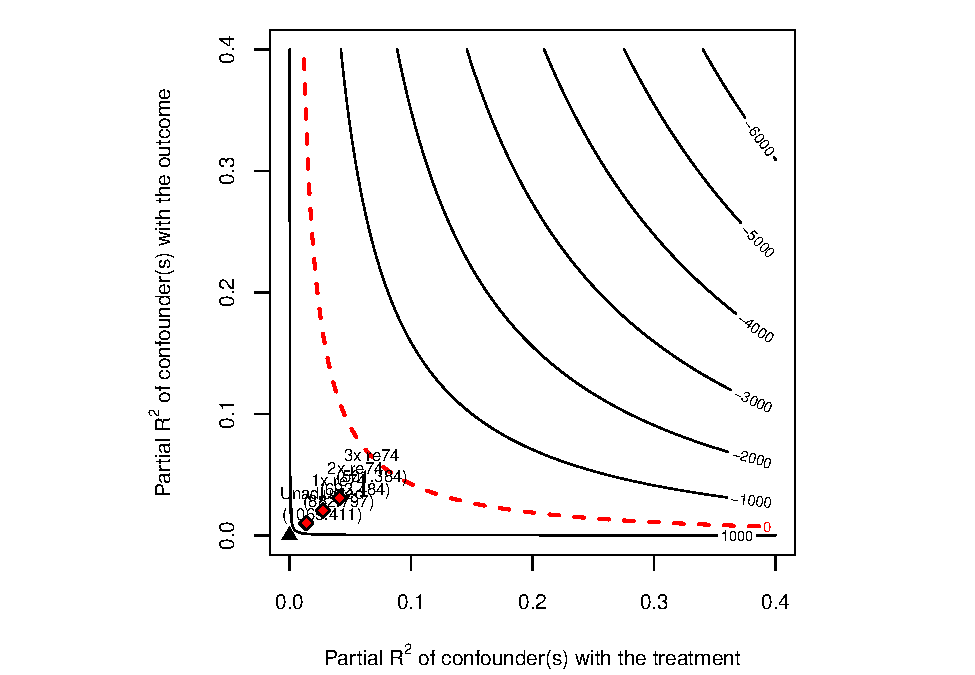
\includegraphics[keepaspectratio]{bookdownproj_files/figure-latex/sensemakr-lalonde-1.pdf}}

O gráfico mostra as combinações de força do confounder (em termos de \(R^2\) parcial com o tratamento e com o resultado) que anulariam o efeito estimado. As linhas de \emph{benchmark} mostram onde estariam confounders com a mesma força explicativa que \texttt{re74} --- uma das covariáveis mais importantes. Se o confounder precisaria ser muito mais forte que qualquer covariável observada para invalidar o resultado, isso indica robustez.

\subsection{Matching e Diferença em Diferenças}\label{matching-e-diferenuxe7a-em-diferenuxe7as}

Uma conexão importante entre matching e outros métodos de inferência causal é o uso de propensity scores e matching em estimadores de Diferença em Diferenças (DiD). O estimador de Callaway and Sant'Anna (\citeproc{ref-callawaysantanna2021}{2021}) para DiD com tratamento escalonado (\emph{staggered treatment}), implementado no pacote \texttt{did} em R, utiliza propensity score e outcome regression ``por baixo dos panos'' para construir estimadores duplamente robustos (\emph{doubly robust}) do ATT em cada par grupo-período.

A ideia é a seguinte: em vez de simplesmente comparar médias antes e depois entre tratados e controles (como no DiD clássico), o estimador de Callaway e Sant'Anna repesa as unidades do grupo de controle usando o propensity score (estimado via logit com covariáveis pré-tratamento), de modo que o grupo de controle repesado se assemelhe ao grupo tratado nas covariáveis. Essa repesagem é combinada com uma regressão do outcome, produzindo um estimador que é consistente se \emph{pelo menos um} dos dois modelos (propensity score ou outcome regression) estiver correto --- daí a propriedade de dupla robustez.

Isso mostra que matching e propensity scores não são apenas ferramentas para estudos cross-section: eles desempenham um papel central em métodos modernos de painel, melhorando a plausibilidade da hipótese de tendências paralelas condicionais.

\subsection{Conclusão}\label{conclusuxe3o}

\textbf{Para refletir:} todos os métodos deste capítulo dependem da suposição de que observamos \emph{todas} as variáveis relevantes (CIA). Na prática, como saber se essa suposição é razoável? A análise de sensibilidade (\texttt{sensemakr}, Rosenbaum bounds) ajuda a quantificar a fragilidade, mas não prova que a suposição é verdadeira. Quando você escolheria matching sobre IPW? E quando usaria estimadores duplamente robustos?

Em resumo, matching é uma ferramenta poderosa para estimar efeitos causais em estudos observacionais, mas requer atenção ao balanceamento, à escolha do método e à plausibilidade da suposição de independência condicional. Métodos modernos como CEM e entropy balancing oferecem melhorias importantes sobre o matching por nearest-neighbor tradicional. E a análise de sensibilidade é uma boa prática indispensável para avaliar a robustez dos resultados a confundimento oculto. No próximo capítulo, veremos uma abordagem alternativa --- variáveis instrumentais --- que permite a identificação causal mesmo quando a seleção em observáveis não é crível.

\section{Variáveis Instrumentais}\label{variuxe1veis-instrumentais}

\subsection{Introdução}\label{introduuxe7uxe3o-5}

O risco de ser convocado para uma guerra muda as atitudes políticas de quem o enfrenta? A pergunta atravessa décadas de debate sobre formação política e juventude. A resposta tentadora seria comparar quem foi convocado com quem não foi, ou quem combateu com quem não combateu. Mas essas populações diferem em classe, escolaridade, região e disposições prévias: quem se alistou voluntariamente, quem ficou de fora por dispensa estudantil ou médica, quem pôde pagar pela faculdade para evitar a convocação. Uma simples diferença de média confunde o efeito do risco com tudo que distinguia os indivíduos antes dele.

Em 1º de dezembro de 1969, no auge da Guerra do Vietnã, o governo americano sorteou em televisão nacional a ordem de convocação dos jovens em idade de servir. Cada data de nascimento recebeu um número de 1 a 366; números baixos eram chamados primeiro, números altos escapariam. Erikson and Stoker (\citeproc{ref-erikson2011}{2011}) usam o número sorteado como instrumento para a \emph{vulnerabilidade} à convocação, em vez de para o serviço militar efetivo: o que importa é a expectativa de poder ser chamado a servir, antes mesmo de o chamado se concretizar. O número é aleatório por design, afeta a probabilidade percebida de ser convocado, e não tem motivo plausível para afetar atitudes décadas depois por outro canal. O resultado: jovens com números baixos se tornaram mais antiguerra, mais liberais e mais propensos a se identificar com o Partido Democrata. O efeito persiste em entrevistas décadas depois e não é mediado pelo serviço militar efetivo: a transformação política veio do risco percebido, não do combate.

Essa é a lógica das variáveis instrumentais. O restante do capítulo desenvolve as condições sob as quais ela funciona: começa pela formulação em DAGs, passa pelo modelo estrutural e pelos mínimos quadrados em dois estágios, e termina sob heterogeneidade de efeitos, em que VI identifica o LATE, o efeito médio sobre quem responde ao instrumento.

Considere o seguinte DAG canônico de Variáveis Instrumentais:

\pandocbounded{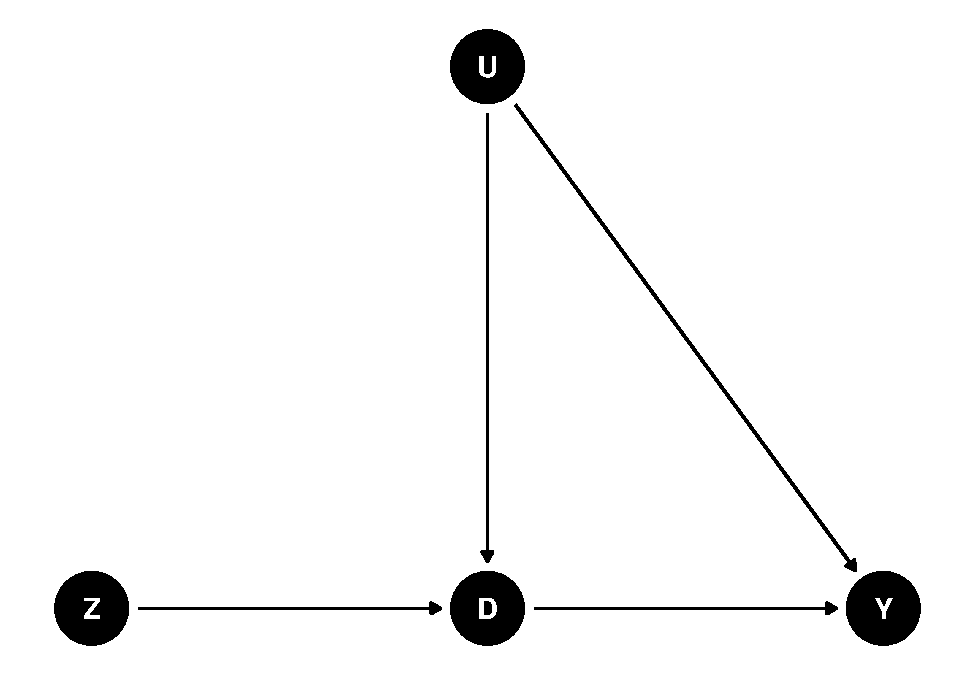
\includegraphics[keepaspectratio]{bookdownproj_files/figure-latex/dag-diagram1-1.pdf}}

Nós vemos que o efeito causal do tratamento \(D\) é confundido pela variável não observada \(U\), já que temos um \emph{backdoor} aberto. Porém, a variável \(Z\) não tem nenhum caminho aberto para \(Y\) exceto via \(D\), isto é, \(D\) é um mediador do efeito causal de \(Z\).

Do ponto de vista não paramétrico (DAGs), dizemos que a variável \(Z\) é uma \textbf{candidata} a variável instrumental (IV) se:

\begin{enumerate}
\def\labelenumi{\arabic{enumi}.}
\item
  \(Z\) está conectado a \(D\) no grafo original. Condição de \textbf{relevância}.
\item
  No grafo em que a seta de \(D\) para \(y\) é removida, \(Z\) é d-separado de \(Y\). \textbf{Exclusion Restriction}.
\item
  A variável instrumental \(Z\) não compartilha causa comum com \(Y\), incluindo, portanto, não ser descendente de \(D\). \textbf{Causa comum}.
\end{enumerate}

Em alguns casos, é necessário controlar para um conjunto de covariáveis \(X\) para que a segunda condição seja satisfeita; chamamos isso de IV condicional. Note também que dizemos que \(Z\) é apenas uma \textbf{candidata} a instrumento porque as três condições acima, embora necessárias, não são suficientes --- discutiremos adiante o que mais é preciso (em particular, monotonicidade, sob heterogeneidade de efeitos).

A literatura econométrica às vezes formula a condição 3 dizendo que \(Z\) deve \emph{causar} \(D\). A direção da implicação é correta: se \(Z\) causa \(D\) e é tratado como exógeno, segue-se que \(Z\) e \(Y\) não compartilham causa comum, validando a condição 3. A volta é falsa: VI não exige que \(Z\) cause \(D\). Manter as condições 2 (exclusão) e 3 (causa comum) separadas torna esse ponto visível, porque a condição 2 fecha caminhos diretos de \(Z\) para \(Y\) e a condição 3 fecha caminhos por confundimento, sem que nenhuma das duas exija causalidade \(Z \to D\). O DAG abaixo mostra um caso em que \(Z\) não causa \(D\) e ainda assim é VI candidata: condicionando em \(V_3\), um collider entre \(Z\) e \(D\), induz-se a correlação que satisfaz a relevância sem violar a condição 3.

\pandocbounded{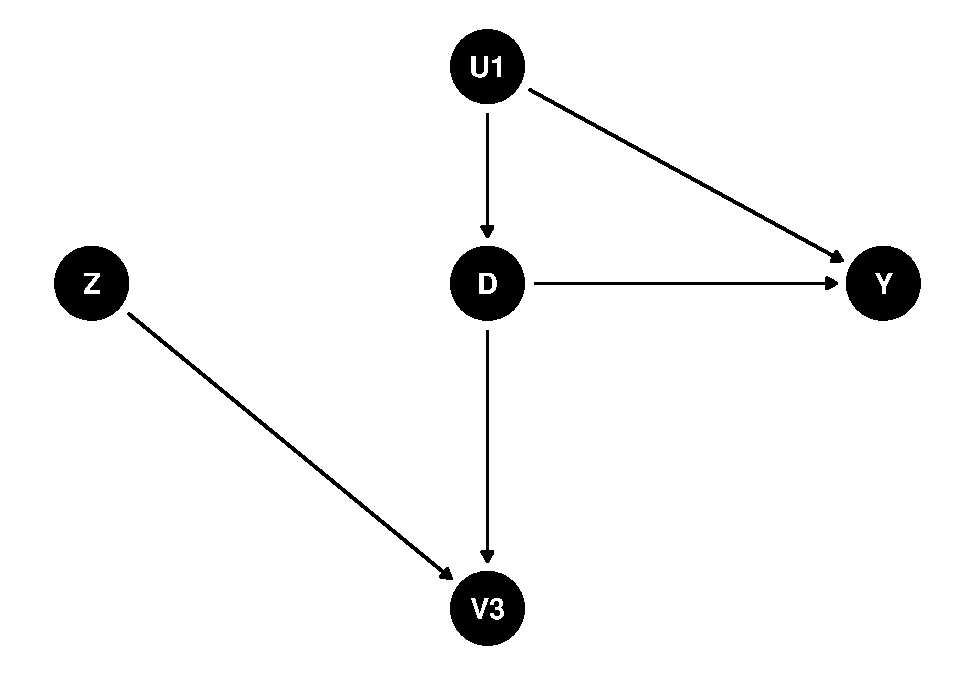
\includegraphics[keepaspectratio]{bookdownproj_files/figure-latex/dag-diagram2-1.pdf}}

Do mesmo jeito, se \(V_3\) for causa comum de \(Z\) e \(D\), não controlar para ela torna \(Z\) admissível como VI.

\pandocbounded{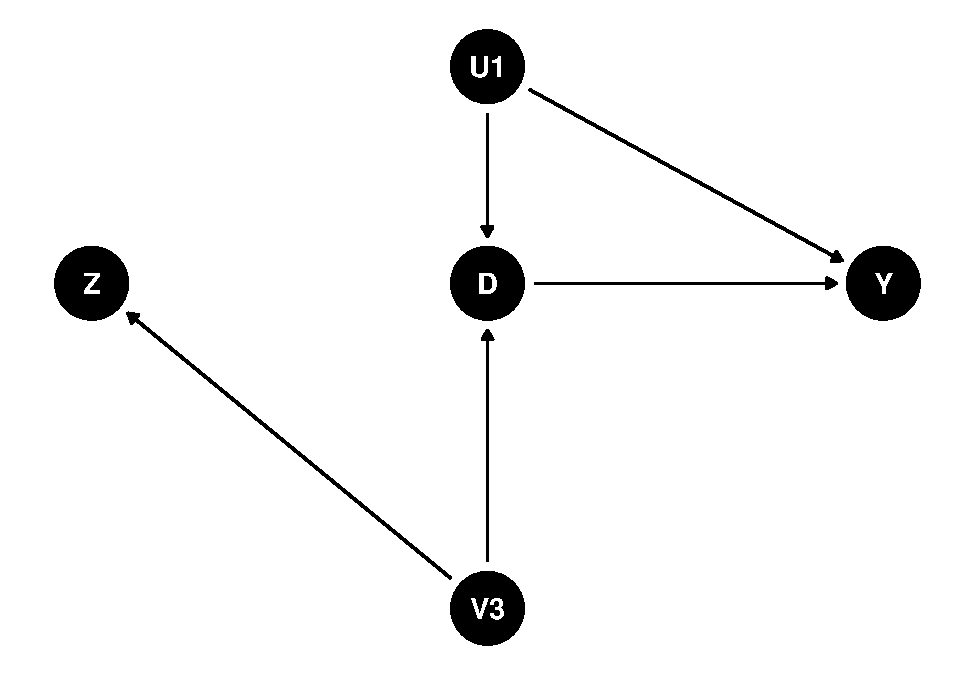
\includegraphics[keepaspectratio]{bookdownproj_files/figure-latex/dag-diagram3-1.pdf}}

Será que \(Z\) pode ser uma IV no DAG abaixo?

\pandocbounded{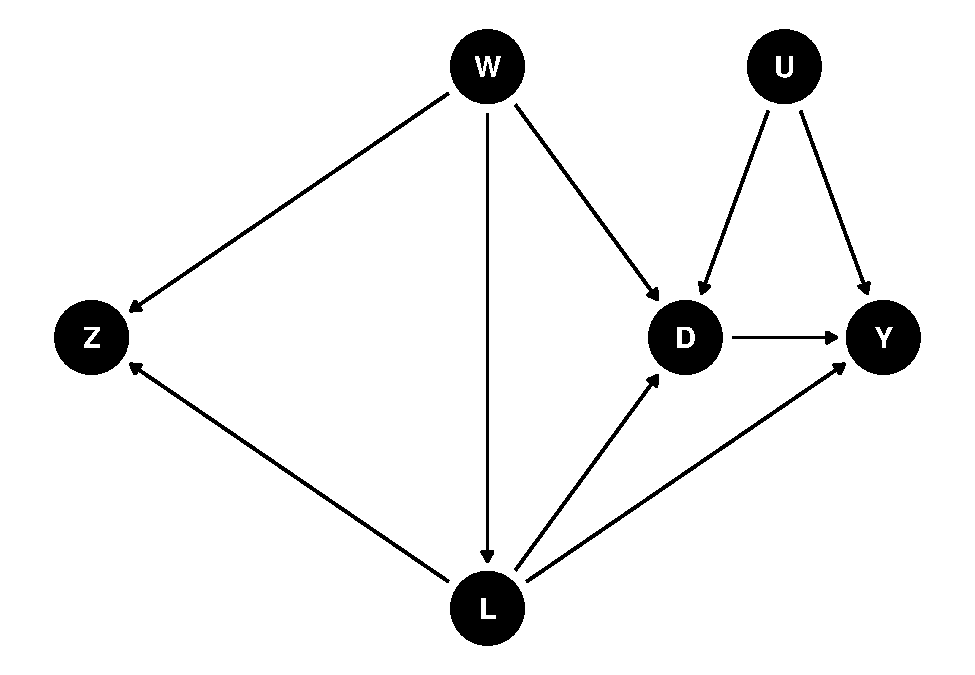
\includegraphics[keepaspectratio]{bookdownproj_files/figure-latex/dag-diagram4-1.pdf}}

Vamos verificar as condições. É fácil ver que \(Z\) está conectado a \(D\), já que temos dois caminhos abertos, um via \(W\) e outro via \(L\) (e ainda um via \(W\) via \(L\)). Portanto, a primeira condição está satisfeita. Note que se eu controlar simultaneamente para \(W\) e \(L\), então eu fecho todos os caminhos abertos.

Com relação à segunda condição, remover a flecha de \(D\) para \(Y\) é, efetivamente, ter um novo DAG:

\pandocbounded{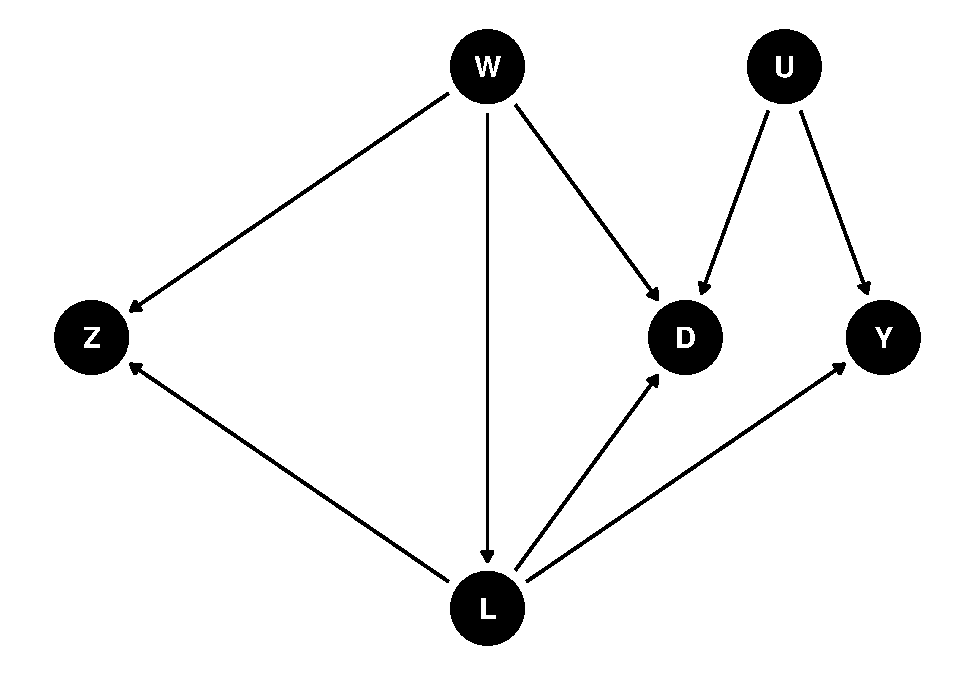
\includegraphics[keepaspectratio]{bookdownproj_files/figure-latex/dag-diagram4-mod-1.pdf}}

Por fim, \(Z\) não compartilha causa comum com \(Y\).

Nesse DAG, \(Z\) não está d-separado de \(Y\), pois existe um caminho aberto para \(Y\) via \(L\). Portanto, controlando para \(L\) (mas não \(W\)), tenho um instrumento que passa nas duas condições.

Até aqui vimos as condições para que uma variável seja candidata a instrumento a partir da perspectiva de DAGs. Vejamos agora como essas condições se traduzem em um modelo estrutural paramétrico.

\subsection{IV com modelo estrutural}\label{iv-com-modelo-estrutural}

A perspectiva em DAGs nos diz quando uma variável é candidata a IV. Para \emph{estimar} o efeito causal, precisamos de uma representação paramétrica. O modelo estrutural canônico de IV escreve duas equações simultâneas, uma para o resultado e outra para o tratamento, com uma variável não observada \(U\) entrando em ambas:

\begin{equation}
\begin{aligned}
y_i &= \beta D_i + \delta_2 U + e_i \\
D_i &= \delta_1 U + \pi z_i + u_i
\end{aligned}
\label{eq:estrutural}
\end{equation}

As duas equações são \emph{estruturais}: representam relações causais, não apenas associações estatísticas. O parâmetro de interesse é \(\beta\), o efeito causal de \(D\) sobre \(Y\). Para identificá-lo via MQO da equação de \(y\), precisaríamos da exogeneidade do tratamento, \(\mathbb{E}[e_i \mid D_i] = 0\). Essa condição falha: \(D_i\) é endógeno porque \(U\) aparece nas duas equações. Esse é o viés de variável omitida que o DAG canônico mostra graficamente, com o backdoor \(D \leftarrow U \to Y\) contaminando a estimativa de \(\beta\).

O instrumento \(z_i\), por construção, entra na equação de \(D_i\) mas não na equação de \(y_i\). Essa ausência é a restrição de exclusão: \(z\) está excluído do RHS da equação de \(Y\). Sob este modelo, a hipótese se traduz operacionalmente em \(\mathbb{E}[z_i \, e_i] = 0\), ou seja, o instrumento é não-correlacionado com o erro estrutural de \(Y\). O coeficiente \(\pi\) na equação de \(D_i\) é o efeito causal do instrumento sobre o tratamento --- o \emph{primeiro estágio} --- e sua positividade é a condição de relevância.

Suponha, para simplificar, que \(D_i\) e \(z_i\) são binários. Nesse caso, uma diferença simples de média identifica \(\pi\):

\[\hat{\pi} = \bar{D}_{\{Z=1\}} - \bar{D}_{\{Z=0\}} = \frac{\sum_{i} z_i D_i}{\sum_{i} z_i} - \frac{\sum_{i} (1-z_i) D_i}{\sum_{i} (1-z_i)}.\]

Mas \(\hat\pi\) é o efeito do \emph{instrumento} sobre o \emph{tratamento}, não o efeito do tratamento sobre o resultado. O que queremos é \(\beta\). Para chegar lá, precisamos de uma estratégia que use \(z\) para isolar a parte exógena de \(D\) e use essa parte para identificar \(\beta\). Essa estratégia é a regressão em dois estágios.

\subsection{MQO em 2 Estágios}\label{mqo-em-2-estuxe1gios}

Considere novamente o DAG canônico para IV. Como poderíamos estimar o efeito causal de \(D\) sobre \(Y\)?

Uma possibilidade é a chamada forma reduzida, que pode ser derivada a partir da suposição de independência. Antes, vamos introduzir uma notação:

A notação \(Y_i(d, z)\) indica o resultado potencial da unidade \(i\) se ela recebesse tratamento \(d\) e valor \(z\) do instrumento. Sob a restrição de exclusão (Seção \ref{restricao-de-exclusao}), \(Y_i(d, z) = Y_i(d, z')\) para todo \(z, z'\), e a notação simplifica para \(Y_i(d)\). Adotamos \(Y_i(d)\) no que segue, com os valores específicos \(Y_i(0)\) e \(Y_i(1)\).

E também temos um status potencial do tratamento (em oposição ao tratamento observado): \(D^1_i\) é o status do tratamento quando \(Z=1\). Similarmente, \(D^0_i\) é o status do tratamento quando \(Z=0\).

E aqui temos uma nova \emph{switching equation}:

\[D_i = D^0_i + (D^1_i - D^0_i)Z_i\]

\begin{align}
   E\big[Y_i\mid Z_i=1\big]-E\big[Y_i\mid Z_i=0\big] & = E\big[Y_i(D_i^1,1)\mid Z_i=1\big]-
   E\big[Y_i(D_i^0,0)\mid Z_i=0\big]
   \\
                                    & = E[Y_i(D_i^1,1)] - E[Y_i(D_i^0,0)]  
\end{align}

O estimador é o efeito causal (total) de \(Z\) sobre \(Y\). Em um experimento, isso é chamado de \emph{intent to treat}, pois se a aleatorização é o instrumento, então é o efeito causal da intenção de tratar.

\begin{Shaded}
\begin{Highlighting}[]
\FunctionTok{library}\NormalTok{(stargazer)}

\NormalTok{n }\OtherTok{\textless{}{-}} \DecValTok{100000}

\FunctionTok{set.seed}\NormalTok{(}\DecValTok{123}\NormalTok{)}
\NormalTok{z }\OtherTok{\textless{}{-}} \FunctionTok{rnorm}\NormalTok{(n)}
\NormalTok{u }\OtherTok{\textless{}{-}} \FunctionTok{rnorm}\NormalTok{(n, }\DecValTok{0}\NormalTok{ , }\DecValTok{3}\NormalTok{)}
\NormalTok{treatment }\OtherTok{\textless{}{-}} \FunctionTok{rbinom}\NormalTok{(n, }\DecValTok{1}\NormalTok{, }\FunctionTok{plogis}\NormalTok{(z }\SpecialCharTok{{-}}\NormalTok{ u }\SpecialCharTok{+} \FunctionTok{rnorm}\NormalTok{(n, }\DecValTok{0}\NormalTok{, }\DecValTok{2}\NormalTok{)))}

\NormalTok{y }\OtherTok{\textless{}{-}} \DecValTok{2}\SpecialCharTok{*}\NormalTok{treatment }\SpecialCharTok{+}\NormalTok{ u}

\NormalTok{reg\_vies }\OtherTok{\textless{}{-}} \FunctionTok{lm}\NormalTok{(y }\SpecialCharTok{\textasciitilde{}}\NormalTok{ treatment)}
\NormalTok{reg\_1s   }\OtherTok{\textless{}{-}} \FunctionTok{lm}\NormalTok{(treatment }\SpecialCharTok{\textasciitilde{}}\NormalTok{ z)}
\NormalTok{reg\_2s   }\OtherTok{\textless{}{-}} \FunctionTok{lm}\NormalTok{(y }\SpecialCharTok{\textasciitilde{}} \FunctionTok{fitted}\NormalTok{(reg\_1s))}

\FunctionTok{stargazer}\NormalTok{(reg\_vies, reg\_1s, reg\_2s,}
          \AttributeTok{type =} \FunctionTok{ifelse}\NormalTok{(knitr}\SpecialCharTok{::}\FunctionTok{is\_html\_output}\NormalTok{(), }\StringTok{"html"}\NormalTok{, }\StringTok{"latex"}\NormalTok{),}
          \AttributeTok{title =} \StringTok{"OLS e 2SLS"}\NormalTok{)}
\end{Highlighting}
\end{Shaded}

\% Table created by stargazer v.5.2.3 by Marek Hlavac, Social Policy Institute. E-mail: marek.hlavac at gmail.com
\% Date and time: Thu, Jun 11, 2026 - 12:38:46

\begin{table}[!htbp] \centering 
  \caption{OLS e 2SLS} 
  \label{} 
\begin{tabular}{@{\extracolsep{5pt}}lccc} 
\\[-1.8ex]\hline 
\hline \\[-1.8ex] 
 & \multicolumn{3}{c}{\textit{Dependent variable:}} \\ 
\cline{2-4} 
\\[-1.8ex] & y & treatment & y \\ 
\\[-1.8ex] & (1) & (2) & (3)\\ 
\hline \\[-1.8ex] 
 treatment & $-$1.495$^{***}$ &  &  \\ 
  & (0.016) &  &  \\ 
  & & & \\ 
 z &  & 0.095$^{***}$ &  \\ 
  &  & (0.002) &  \\ 
  & & & \\ 
 fitted(reg\_1s) &  &  & 1.916$^{***}$ \\ 
  &  &  & (0.085) \\ 
  & & & \\ 
 Constant & 1.760$^{***}$ & 0.499$^{***}$ & 0.058 \\ 
  & (0.011) & (0.002) & (0.043) \\ 
  & & & \\ 
\hline \\[-1.8ex] 
Observations & 100,000 & 100,000 & 100,000 \\ 
R$^{2}$ & 0.085 & 0.036 & 0.005 \\ 
Adjusted R$^{2}$ & 0.085 & 0.036 & 0.005 \\ 
Residual Std. Error (df = 99998) & 2.453 & 0.491 & 2.558 \\ 
F Statistic (df = 1; 99998) & 9,283.268$^{***}$ & 3,739.184$^{***}$ & 505.426$^{***}$ \\ 
\hline 
\hline \\[-1.8ex] 
\textit{Note:}  & \multicolumn{3}{r}{$^{*}$p$<$0.1; $^{**}$p$<$0.05; $^{***}$p$<$0.01} \\ 
\end{tabular} 
\end{table}

A primeira coluna traz a regressão ingênua de \(Y\) sobre \(D\): o coeficiente está viesado porque \(U\) afeta \(D\) e \(Y\) ao mesmo tempo, e a covariância induzida puxa a estimativa para longe do efeito verdadeiro \(\beta = 2\) usado na simulação. A segunda coluna é o primeiro estágio: \(Z\) desloca \(D\) na direção esperada. A terceira coluna regrede \(Y\) sobre \(\hat{D}\), a parte de \(D\) projetada sobre \(Z\), e recupera um coeficiente próximo de \(2\). A diferença entre a primeira e a terceira coluna é o viés que VI corrige.

\begin{Shaded}
\begin{Highlighting}[]
\FunctionTok{library}\NormalTok{(tidyverse)}
\FunctionTok{library}\NormalTok{(ggplot2)}

\NormalTok{simulate\_and\_fit }\OtherTok{\textless{}{-}} \ControlFlowTok{function}\NormalTok{(n) \{}
\NormalTok{  z }\OtherTok{\textless{}{-}} \FunctionTok{rnorm}\NormalTok{(n)}
\NormalTok{  u }\OtherTok{\textless{}{-}} \FunctionTok{rnorm}\NormalTok{(n, }\DecValTok{0}\NormalTok{, }\DecValTok{3}\NormalTok{)}
\NormalTok{  treatment }\OtherTok{\textless{}{-}} \FunctionTok{rbinom}\NormalTok{(n, }\DecValTok{1}\NormalTok{, }\FunctionTok{plogis}\NormalTok{(z }\SpecialCharTok{{-}}\NormalTok{ u }\SpecialCharTok{+} \FunctionTok{rnorm}\NormalTok{(n, }\DecValTok{0}\NormalTok{, }\DecValTok{2}\NormalTok{)))}
\NormalTok{  y }\OtherTok{\textless{}{-}} \DecValTok{2} \SpecialCharTok{*}\NormalTok{ treatment }\SpecialCharTok{+}\NormalTok{ u}
  
  \CommentTok{\# Naive regression}
\NormalTok{  reg\_vies }\OtherTok{\textless{}{-}} \FunctionTok{lm}\NormalTok{(y }\SpecialCharTok{\textasciitilde{}}\NormalTok{ treatment)}
  
  \CommentTok{\# 2SLS}
\NormalTok{  reg\_1s }\OtherTok{\textless{}{-}} \FunctionTok{lm}\NormalTok{(treatment }\SpecialCharTok{\textasciitilde{}}\NormalTok{ z)}
\NormalTok{  predicted\_treatment }\OtherTok{\textless{}{-}} \FunctionTok{predict}\NormalTok{(reg\_1s)}
\NormalTok{  reg\_2s }\OtherTok{\textless{}{-}} \FunctionTok{lm}\NormalTok{(y }\SpecialCharTok{\textasciitilde{}}\NormalTok{ predicted\_treatment)}
  
  \CommentTok{\# Return coefficients}
  \FunctionTok{tibble}\NormalTok{(}
    \AttributeTok{naive\_coef =} \FunctionTok{coef}\NormalTok{(reg\_vies)[}\DecValTok{2}\NormalTok{],}
    \AttributeTok{tsls\_coef =} \FunctionTok{coef}\NormalTok{(reg\_2s)[}\DecValTok{2}\NormalTok{]}
\NormalTok{  )}
\NormalTok{\}}


\CommentTok{\# Sample sizes to simulate}
\NormalTok{sample\_sizes }\OtherTok{\textless{}{-}} \FunctionTok{seq}\NormalTok{(}\DecValTok{1000}\NormalTok{, }\DecValTok{100000}\NormalTok{, }\AttributeTok{by =} \DecValTok{1000}\NormalTok{)}

\CommentTok{\# Use map to apply the function to each sample size}
\NormalTok{results }\OtherTok{\textless{}{-}} \FunctionTok{tibble}\NormalTok{(}\AttributeTok{sample\_size =}\NormalTok{ sample\_sizes) }\SpecialCharTok{\%\textgreater{}\%}
  \FunctionTok{mutate}\NormalTok{(}
    \AttributeTok{simulation\_results =} \FunctionTok{map}\NormalTok{(sample\_size, simulate\_and\_fit)}
\NormalTok{  ) }\SpecialCharTok{\%\textgreater{}\%}
  \FunctionTok{unnest}\NormalTok{(}\AttributeTok{cols =} \FunctionTok{c}\NormalTok{(simulation\_results))}

\NormalTok{results }\SpecialCharTok{\%\textgreater{}\%}
  \FunctionTok{pivot\_longer}\NormalTok{(}\AttributeTok{cols =} \FunctionTok{c}\NormalTok{(naive\_coef, tsls\_coef), }\AttributeTok{names\_to =} \StringTok{"method"}\NormalTok{, }\AttributeTok{values\_to =} \StringTok{"coefficient"}\NormalTok{) }\SpecialCharTok{\%\textgreater{}\%}
  \FunctionTok{ggplot}\NormalTok{(}\FunctionTok{aes}\NormalTok{(}\AttributeTok{x =}\NormalTok{ sample\_size, }\AttributeTok{y =}\NormalTok{ coefficient, }\AttributeTok{color =}\NormalTok{ method)) }\SpecialCharTok{+}
  \FunctionTok{geom\_line}\NormalTok{() }\SpecialCharTok{+}
  \FunctionTok{geom\_smooth}\NormalTok{(}\AttributeTok{data =}\NormalTok{ . }\SpecialCharTok{\%\textgreater{}\%} \FunctionTok{filter}\NormalTok{(method }\SpecialCharTok{==} \StringTok{"tsls\_coef"}\NormalTok{), }\AttributeTok{method =} \StringTok{"lm"}\NormalTok{, }\AttributeTok{se =} \ConstantTok{FALSE}\NormalTok{, }\AttributeTok{color =} \StringTok{"red"}\NormalTok{) }\SpecialCharTok{+}

  \FunctionTok{labs}\NormalTok{(}
    \AttributeTok{title =} \StringTok{"Convergência dos coeficientes com o tamanho da amostra"}\NormalTok{,}
    \AttributeTok{x =} \StringTok{"Tamanho da amostra"}\NormalTok{,}
    \AttributeTok{y =} \StringTok{"Coeficiente estimado"}\NormalTok{,}
    \AttributeTok{color =} \StringTok{"Método"}
\NormalTok{  ) }\SpecialCharTok{+}
  \FunctionTok{theme\_minimal}\NormalTok{() }\SpecialCharTok{+}
  \FunctionTok{scale\_color\_manual}\NormalTok{(}
    \AttributeTok{values =} \FunctionTok{c}\NormalTok{(}\StringTok{"naive\_coef"} \OtherTok{=} \StringTok{"blue"}\NormalTok{, }\StringTok{"tsls\_coef"} \OtherTok{=} \StringTok{"red"}\NormalTok{),}
    \AttributeTok{labels =} \FunctionTok{c}\NormalTok{(}\StringTok{"naive\_coef"} \OtherTok{=} \StringTok{"MQO ingênuo"}\NormalTok{, }\StringTok{"tsls\_coef"} \OtherTok{=} \StringTok{"2SLS"}\NormalTok{)}
\NormalTok{  ) }\SpecialCharTok{+}
  \FunctionTok{theme}\NormalTok{(}
    \AttributeTok{plot.title =} \FunctionTok{element\_text}\NormalTok{(}\AttributeTok{hjust =} \FloatTok{0.5}\NormalTok{),}
    \AttributeTok{legend.title =} \FunctionTok{element\_blank}\NormalTok{()}
\NormalTok{  )}
\end{Highlighting}
\end{Shaded}

\begin{verbatim}
## `geom_smooth()` using formula = 'y ~ x'
\end{verbatim}

\pandocbounded{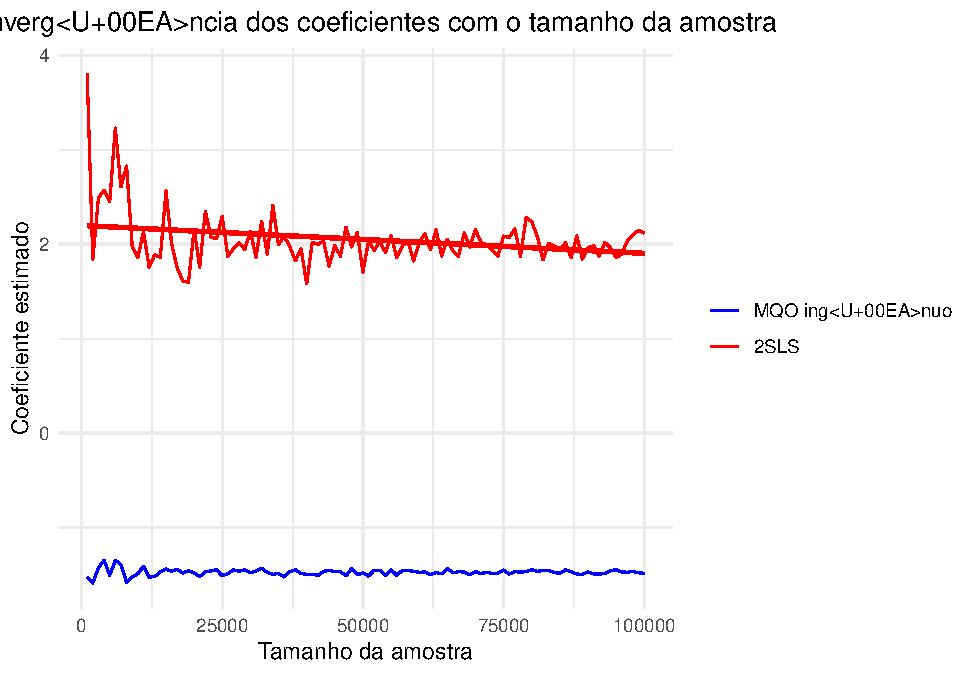
\includegraphics[keepaspectratio]{bookdownproj_files/figure-latex/sim-dag-canonico-n-1.pdf}}

A leitura do gráfico mostra duas trajetórias bem distintas. A curva azul (MQO ingênuo) estabiliza em torno de um valor menor que \(\beta = 2\) --- esse é o viés de variável omitida, que não desaparece com \(n\) porque o problema é de identificação, não de variância amostral. A curva vermelha (2SLS) oscila mais para amostras pequenas (a divisão por \(\hat\pi\) ruidoso amplifica o erro), mas converge para \(2\) conforme \(n\) cresce. O ponto pedagógico: \(n\) grande não corrige viés se a estratégia de identificação está errada; corrige apenas variância dado uma estratégia válida.

\subsection{Efeito heterogêneo}\label{efeito-heteroguxeaneo}

Os resultados anteriores supuseram que o efeito do tratamento é homogêneo: \(Y_i(1) - Y_i(0) = \beta\) para toda unidade \(i\). Quando o efeito varia entre indivíduos, o que IV identifica deixa de ser o ATE --- passa a ser um efeito médio sobre um subgrupo específico, definido pelo próprio instrumento.

Para discutir efeito causal heterogêneo, vamos utilizar um estudo em ciência política (\citeproc{ref-white2019}{White 2019}). Qual é o efeito de uma condenação por \emph{misdemeanor} (algo como contravenção penal) sobre comparecimento eleitoral? O autor argumenta que o efeito deve variar por raça (maior para negros que brancos), de modo que o efeito causal é heterogêneo. Segundo o autor, casos são atribuídos aleatoriamente a diferentes cortes judiciais, e elas variam em sua leniência. Aqui, o tratamento é a condenação (\(D_i = 1\) se condenado, \(0\) caso contrário), e o instrumento é o sorteio de um juiz mais ou menos leniente.

Formalmente, o efeito causal heterogêneo é \(\delta_i = Y_i(1) - Y_i(0)\). Nesse caso, não podemos mais estimar o efeito causal médio populacional (ATE), porque o instrumento só explica variação no tratamento para um subgrupo da população: os \emph{compliers}. Antes de derivar o estimador, vale fixar o vocabulário.

\subsection{Tipologia de unidades}\label{tipologia-de-unidades}

Sob um instrumento binário \(Z_i \in \{0, 1\}\), cada unidade tem dois status potenciais de tratamento, \(D^0_i\) (se \(Z_i = 0\)) e \(D^1_i\) (se \(Z_i = 1\)). A combinação dos dois define quatro tipos:

\begin{longtable}[]{@{}lll@{}}
\toprule\noalign{}
& \(D^0_i = 0\) & \(D^0_i = 1\) \\
\midrule\noalign{}
\endhead
\bottomrule\noalign{}
\endlastfoot
\(D^1_i = 0\) & \textbf{never-takers} & \textbf{defiers} \\
\(D^1_i = 1\) & \textbf{compliers} & \textbf{always-takers} \\
\end{longtable}

No estudo de White (\citeproc{ref-white2019}{2019}):

\begin{itemize}
\tightlist
\item
  \textbf{Always-takers} são acusados que serão condenados qualquer que seja o juiz sorteado --- em geral aqueles com forte conjunto de evidências contra si.
\item
  \textbf{Never-takers} são acusados que serão absolvidos qualquer que seja o juiz --- em geral aqueles com poucas evidências.
\item
  \textbf{Compliers} são acusados cuja condenação responde ao instrumento: condenados se enviados ao juiz severo, absolvidos se enviados ao leniente.
\item
  \textbf{Defiers} seriam acusados que fariam o oposto: absolvidos pelo juiz severo e condenados pelo leniente. Substantivamente, isso não faz sentido no contexto, mas teoricamente é uma possibilidade que precisa ser excluída por hipótese.
\end{itemize}

Apenas o subgrupo dos compliers fornece variação útil para identificar efeito causal a partir do instrumento. Para always- e never-takers, o instrumento não move o tratamento; para defiers, move-o na direção contrária. As suposições adicionais a seguir excluem defiers da população e isolam o efeito local sobre os compliers.

\subsection{Suposições para o LATE}\label{suposiuxe7uxf5es-para-o-late}

\subsubsection{SUTVA}\label{sutva}

Resultados potenciais para a unidade \(i\) não dependem do tratamento recebido por \(j\). Há potencial para SUTVA ser violada no estudo de encarceramento e voto: se dois irmãos (\(i\) e \(j\)) são acusados e um deles é preso, o tratamento de um pode impactar a probabilidade de voto do outro. White não discute explicitamente essa possibilidade. Vamos supor, porém, que SUTVA esteja garantido.

\subsubsection{Independência}\label{independuxeancia}

Também chamada de \emph{as good as random assignment} ou \emph{no confounding for the effect of \(Z\) on \(Y\)}: o instrumento é independente dos resultados potenciais \(Y_i(d)\) e dos status potenciais de tratamento \(D^z_i\). No estudo de White, a aleatorização da corte sustenta essa hipótese: é difícil imaginar variável que cause a leniência judicial e simultaneamente o comparecimento eleitoral.

Vale tornar o mapeamento entre as duas formulações de IV explícito. Cada uma das três suposições não-paramétricas vistas no início do capítulo tem uma contrapartida em resultados potenciais (Tabela \ref{tab:dag-vs-po}).

\begin{longtable}[]{@{}
  >{\raggedright\arraybackslash}p{(\linewidth - 4\tabcolsep) * \real{0.1450}}
  >{\raggedright\arraybackslash}p{(\linewidth - 4\tabcolsep) * \real{0.3817}}
  >{\raggedright\arraybackslash}p{(\linewidth - 4\tabcolsep) * \real{0.4733}}@{}}
\caption{\label{tab:dag-vs-po} Mapeamento entre as condições de IV em DAG e em resultados potenciais.}\tabularnewline
\toprule\noalign{}
\begin{minipage}[b]{\linewidth}\raggedright
Hipótese
\end{minipage} & \begin{minipage}[b]{\linewidth}\raggedright
DAG
\end{minipage} & \begin{minipage}[b]{\linewidth}\raggedright
Resultados potenciais
\end{minipage} \\
\midrule\noalign{}
\endfirsthead
\toprule\noalign{}
\begin{minipage}[b]{\linewidth}\raggedright
Hipótese
\end{minipage} & \begin{minipage}[b]{\linewidth}\raggedright
DAG
\end{minipage} & \begin{minipage}[b]{\linewidth}\raggedright
Resultados potenciais
\end{minipage} \\
\midrule\noalign{}
\endhead
\bottomrule\noalign{}
\endlastfoot
Relevância & \(Z\) conectado a \(D\) no grafo original & \(\mathbb{E}[D^1_i] \neq \mathbb{E}[D^0_i]\) \\
Exclusão & \(Z\) d-separado de \(Y\) no grafo sem \(D \to Y\) & \(Y_i(d, z) = Y_i(d, z')\) para todo \(i, d, z, z'\) \\
Sem confundimento & \(Z\) não compartilha causa comum com \(Y\) & \(Z_i \perp\!\!\!\perp \{Y_i(d), D^z_i\}\) \\
\end{longtable}

A linha ``sem confundimento'' é onde os dois frameworks divergem. A versão em resultados potenciais é estritamente mais forte: exige independência também em relação aos status potenciais \(D^z_i\), o que excluiria casos como o DAG com causa comum \(V_3\) visto na introdução. Em aplicações típicas \(Z\) é tratado como raiz do DAG (sem parents), e as duas formulações coincidem operacionalmente; adotamos a versão em resultados potenciais para a derivação do LATE adiante.

\subsubsection{Restrição de Exclusão}\label{restricao-de-exclusao}

A restrição de exclusão requer que o instrumento \(Z\) afete o resultado \(Y\) apenas por meio do tratamento \(D\). Não há efeito direto de \(Z\) sobre \(Y\) que não passe por \(D\). A suposição não é testável diretamente: precisa ser justificada com argumentos substantivos sobre o mecanismo.

A literatura formula essa hipótese em três linguagens: estrutural clássica, DAG e resultados potenciais. Sob homogeneidade linear (efeito do tratamento constante), as três são equivalentes. Sob heterogeneidade, a formulação em resultados potenciais distingue exclusão de independência, e essa separação vale conhecer.

\paragraph{Formulação estrutural clássica}\label{formulauxe7uxe3o-estrutural-cluxe1ssica}

No modelo
\[y_i = \beta D_i + \delta_2 U + e_i,\]
a restrição de exclusão é o fato de que \(z_i\) não aparece no RHS desta equação. Sob exogeneidade do erro estrutural, isso se traduz operacionalmente em \(\mathbb{E}[z_i \, e_i] = 0\): o instrumento é não-correlacionado com o erro estrutural de \(Y\). Aqui exclusão e exogeneidade do instrumento ficam empacotadas em uma única condição.

\paragraph{Formulação em DAGs}\label{formulauxe7uxe3o-em-dags}

Tome o DAG canônico e remova a flecha \(D \to Y\). A restrição de exclusão diz que, neste DAG modificado, \(Z\) é d-separado de \(Y\). Não há nenhum caminho aberto entre \(Z\) e \(Y\) uma vez que se deleta o canal via \(D\). A hipótese fica geometricamente legível: se cortar a ponte \(D \to Y\) deixa \(Z\) desconectado de \(Y\) no grafo, a exclusão vale; se sobra algum caminho (por exemplo, \(Z \to W \to Y\)), a exclusão é violada por esse \(W\). Esta talvez seja a formulação mais limpa para o leitor que já está confortável com DAGs.

\paragraph{Formulação em resultados potenciais}\label{formulauxe7uxe3o-em-resultados-potenciais}

Define-se \(Y_i(d, z)\) como o resultado potencial da unidade \(i\) se ela recebesse tratamento \(d\) e valor \(z\) do instrumento. A restrição de exclusão é
\[Y_i(d, z) = Y_i(d, z') \quad \text{para todo } i, d, z, z'.\]
Dado o tratamento, o valor do instrumento não altera o resultado potencial. A notação simplifica para \(Y_i(d)\), como se o instrumento caísse fora da função de resultado potencial.

\paragraph{Exemplo de violação}\label{exemplo-de-violauxe7uxe3o}

O caso clássico é o uso de chuva como instrumento para comparecimento eleitoral. Mellon (\citeproc{ref-mellon2023}{2023}) revisou 289 estudos e identificou 195 variáveis distintas que foram conectadas com chuva na literatura. Qualquer uma delas é candidata a canal direto entre chuva e o resultado de interesse, violando a exclusão. Em DAGs: se chuva afeta humor, e humor afeta voto, há um caminho aberto \(Z \to \text{humor} \to Y\) que não passa por comparecimento.

\subsubsection{Monotonicidade}\label{monotonicidade}

A monotonicidade requer que o instrumento opere (fracamente) na mesma direção para todas as unidades: ele só move pessoas do controle para o tratamento (ou não move ninguém), nunca o contrário. Em outras palavras, não há defiers na população.

Formalmente, \(D^1_i \geq D^0_i\) para todo \(i\). No estudo de White, isso significa que ninguém é condenado pelo juiz leniente \emph{e} absolvido pelo severo --- uma hipótese substantivamente plausível.

\subsection{Identificação do LATE}\label{identificauxe7uxe3o-do-late}

Sob SUTVA, independência, exclusão e monotonicidade, vamos identificar o LATE em três passos: (i) decompor o efeito do instrumento sobre o resultado por tipo de unidade e mostrar que três dos quatro termos zeram; (ii) reescrever a proporção de compliers em termos observáveis; (iii) isolar o LATE.

\subsubsection{Passo 1: decomposição por tipo}\label{passo-1-decomposiuxe7uxe3o-por-tipo}

Partindo de \(\mathbb{E}[Y_i \mid Z_i = 1] - \mathbb{E}[Y_i \mid Z_i = 0]\), sob exclusão e independência o lado direito é igual a \(\mathbb{E}[Y_i(D^1_i) - Y_i(D^0_i)]\). Pela lei da esperança total, condicionando no tipo da unidade:

\begin{align}
  \mathbb{E}[Y_i \mid Z_i = 1] - \mathbb{E}[Y_i \mid Z_i = 0]
   =\;& \mathbb{E}[Y_i(D^1_i) - Y_i(D^0_i) \mid \text{always-takers}] \cdot P(\text{always-takers}) \\
    +& \mathbb{E}[Y_i(D^1_i) - Y_i(D^0_i) \mid \text{never-takers}] \cdot P(\text{never-takers}) \\
    +& \mathbb{E}[Y_i(D^1_i) - Y_i(D^0_i) \mid \text{compliers}] \cdot P(\text{compliers}) \\
    +& \mathbb{E}[Y_i(D^1_i) - Y_i(D^0_i) \mid \text{defiers}] \cdot P(\text{defiers})
\end{align}

onde os tipos são definidos pelos pares \((D^1_i, D^0_i)\) apresentados em §\ref{tipologia-de-unidades}. Para always-takers (\(D^1_i = D^0_i = 1\)) e never-takers (\(D^1_i = D^0_i = 0\)), o integrando é \(Y_i(d) - Y_i(d) = 0\) por construção. Não são as probabilidades que zeram --- always- e never-takers existem com probabilidade positiva; o que zera é o que está dentro da esperança. Para defiers, o integrando não é zero, mas a \emph{probabilidade} zera pela monotonicidade: \(P(\text{defiers}) = P(D^1_i = 0, D^0_i = 1) = 0\). Sobra apenas o termo dos compliers, para os quais \(Y_i(D^1_i) - Y_i(D^0_i) = Y_i(1) - Y_i(0)\):

\begin{equation}
\mathbb{E}[Y_i \mid Z_i = 1] - \mathbb{E}[Y_i \mid Z_i = 0] = \mathbb{E}[Y_i(1) - Y_i(0) \mid \text{complier}] \cdot P(\text{complier}).
\label{eq:itt-complier}
\end{equation}

\subsubsection{\texorpdfstring{Passo 2: identificar \(P(\text{complier})\)}{Passo 2: identificar P(\textbackslash text\{complier\})}}\label{passo-2-identificar-ptextcomplier}

O lado esquerdo de \eqref{eq:itt-complier} é a forma reduzida --- observável diretamente. O primeiro fator do lado direito é o LATE --- o que queremos. Falta o segundo fator, \(P(\text{complier})\). Sob monotonicidade, a partição em tipos satisfaz

\begin{equation}
P(D_i = 1 \mid Z_i = 1) = P(\text{complier}) + P(\text{always-taker})
\label{eq:p-d-z1}
\end{equation}

\begin{equation}
P(D_i = 1 \mid Z_i = 0) = P(\text{always-taker}).
\label{eq:p-d-z0}
\end{equation}

A equação \eqref{eq:p-d-z1} soma always-takers e compliers --- os únicos tipos que recebem \(D = 1\) quando \(Z = 1\). A equação \eqref{eq:p-d-z0} fica só com always-takers, já que defiers foram eliminados pela monotonicidade. Subtraindo \eqref{eq:p-d-z0} de \eqref{eq:p-d-z1}:

\begin{equation}
P(\text{complier}) = P(D_i = 1 \mid Z_i = 1) - P(D_i = 1 \mid Z_i = 0).
\label{eq:p-complier-prob}
\end{equation}

Como \(D_i\) é binário, \(P(D_i = 1 \mid Z_i = z) = \mathbb{E}[D_i \mid Z_i = z]\) (a esperança de uma Bernoulli é a probabilidade do evento). A equação \eqref{eq:p-complier-prob} se reescreve em termos de esperanças observáveis:

\begin{equation}
P(\text{complier}) = \mathbb{E}[D_i \mid Z_i = 1] - \mathbb{E}[D_i \mid Z_i = 0].
\label{eq:p-complier}
\end{equation}

Essa diferença é justamente o \textbf{primeiro estágio} --- o efeito do instrumento sobre o tratamento.

\subsubsection{Passo 3: isolar o LATE}\label{passo-3-isolar-o-late}

Substituindo \eqref{eq:p-complier} em \eqref{eq:itt-complier}, o segundo fator do lado direito vira a diferença observada \(\mathbb{E}[D_i \mid Z_i = 1] - \mathbb{E}[D_i \mid Z_i = 0]\) no lugar de \(P(\text{complier})\):

\begin{equation}
\begin{aligned}
&\mathbb{E}[Y_i \mid Z_i = 1] - \mathbb{E}[Y_i \mid Z_i = 0] \\
&\quad = \mathbb{E}[Y_i(1) - Y_i(0) \mid \text{complier}] \cdot \left( \mathbb{E}[D_i \mid Z_i = 1] - \mathbb{E}[D_i \mid Z_i = 0] \right).
\end{aligned}
\label{eq:itt-first-stage}
\end{equation}

Para isolar o LATE, dividimos os dois lados de \eqref{eq:itt-first-stage} pela diferença \(\mathbb{E}[D_i \mid Z_i = 1] - \mathbb{E}[D_i \mid Z_i = 0]\) --- o primeiro estágio. Sob relevância, esse denominador é diferente de zero, e a divisão é bem definida:

\begin{equation}
\begin{aligned}
\delta_{IV,LATE} &= \mathbb{E}[Y_i(1) - Y_i(0) \mid \text{complier}] \\
                 &= \frac{\mathbb{E}[Y_i \mid Z_i = 1] - \mathbb{E}[Y_i \mid Z_i = 0]}
                         {\mathbb{E}[D_i \mid Z_i = 1] - \mathbb{E}[D_i \mid Z_i = 0]}.
\end{aligned}
\label{eq:wald}
\end{equation}

Este é o \textbf{estimador de Wald}: a razão entre forma reduzida (numerador) e primeiro estágio (denominador). O denominador é a proporção de compliers na população; sua positividade requer relevância --- sem variação induzida em \(D\), o Wald não é definido.

\subsubsection{Localidade do LATE}\label{localidade-do-late}

O LATE é um parâmetro \textbf{local}: refere-se apenas ao subgrupo de compliers, não à população inteira. Essa localidade é simultaneamente uma força e uma limitação. Força: o efeito está bem definido sob suposições críveis e é o que o instrumento de fato identifica. Limitação: quem é complier depende do instrumento --- outro instrumento, outro grupo de compliers, outro LATE --- e o efeito sobre always- e never-takers permanece desconhecido. No estudo de White, o LATE é interpretado substantivamente como o efeito da condenação sobre comparecimento eleitoral \emph{entre acusados marginais}, cuja sentença depende do juiz que pegaram. Vejamos agora questões práticas de estimação.

\subsection{Estimação e força do instrumento}\label{estimauxe7uxe3o-e-foruxe7a-do-instrumento}

\subsubsection{Derivação do estimador 2SLS}\label{derivauxe7uxe3o-do-estimador-2sls}

Considere o modelo simplificado em que as variáveis estão centradas (sem constante) e não há controles:

\begin{equation}
\begin{aligned}
y_i &= \beta D_i + e_i \\
D_i &= \pi z_i + u_i
\end{aligned}
\label{eq:modelo-simples}
\end{equation}

Substituindo a equação do primeiro estágio na equação de resultado, \(y_i\) pode ser expresso em termos de \(z_i\) apenas:

\begin{equation}
\begin{aligned}
y_i &= \beta (\pi z_i + u_i) + e_i \\
    &= \underbrace{\beta \pi}_{\delta}\, z_i + \underbrace{\beta u_i + e_i}_{v_i}.
\end{aligned}
\label{eq:forma-reduzida}
\end{equation}

A equação \eqref{eq:forma-reduzida} é a \emph{forma reduzida}: \(y_i\) projetado diretamente sobre o instrumento \(z_i\), com coeficiente \(\delta = \beta \pi\). A regressão de \(y\) sobre \(z\) identifica \(\hat\delta\); a regressão de \(D\) sobre \(z\) identifica \(\hat\pi\). Como \(\delta = \beta \pi\) na estrutura, segue-se que \(\beta = \delta / \pi\). Substituindo as quantidades populacionais por estimativas:

\begin{equation}
\hat\beta_{2SLS} = \frac{\hat\delta}{\hat\pi}.
\label{eq:beta-2sls}
\end{equation}

Esta é a versão regressiva do estimador de Wald visto na seção anterior: numerador é a forma reduzida, denominador é o primeiro estágio. Equivalentemente, no algoritmo em dois estágios: regrida \(D\) sobre \(z\) para obter \(\hat D = \hat\pi z\); em seguida regrida \(y\) sobre \(\hat D\). O coeficiente da segunda regressão é exatamente \(\hat\delta / \hat\pi\).

\subsubsection{\texorpdfstring{Por que dividir por \(\hat\pi\) é problemático sob instrumento fraco}{Por que dividir por \textbackslash hat\textbackslash pi é problemático sob instrumento fraco}}\label{por-que-dividir-por-hatpi-uxe9-problemuxe1tico-sob-instrumento-fraco}

A divisão por \(\hat\pi\) na equação \eqref{eq:beta-2sls} é o que torna a estimação delicada: quando o primeiro estágio é fraco, \(\hat\pi\) é próximo de zero, e pequenas perturbações em \(\hat\delta\) ou \(\hat\pi\) se amplificam dramaticamente na razão. Sob homocedasticidade, é possível mostrar que o viés de \(\hat\beta_{2SLS}\) em amostras finitas se relaciona com a estatística \(F\) do primeiro estágio segundo

\begin{equation}
\mathbb{E}[\hat\beta_{2SLS} - \beta] \;\approx\; \underbrace{\frac{\text{Cov}(u, e)}{\text{Var}(u)}}_{\text{OVB}} \cdot \frac{k}{F + 1},
\label{eq:vies-2sls}
\end{equation}

onde \(k\) é o número de instrumentos. Se \(F = 0\), o viés é igual ao do MQO ingênuo: VI não corrige nada. Quanto maior \(F\), menor o viés. E quanto mais instrumentos para um mesmo \(F\), maior o viés em amostras finitas.

A regra de bolso clássica é \(F > 10\), devida a Staiger and Stock (\citeproc{ref-staigerstock1997}{1997}) e refinada por Stock and Yogo (\citeproc{ref-stockyogo2005}{2005}): com isso, o viés de 2SLS é inferior a 10\% do viés de MQO com 95\% de confiança. A suposição por trás dessa regra é homocedasticidade. Montiel Olea and Pflueger (\citeproc{ref-montielolea2013}{2013}) desenvolveram um teste robusto a heterocedasticidade que admite clustering e autocorrelação; sob essa estatística \(F\) efetiva, o ponto de corte recomendado sobe para cerca de 23,1.

\subsubsection{Receita prática}\label{receita-pruxe1tica}

Na prática, a estimação 2SLS pode ser feita com \texttt{feols(y\ \textasciitilde{}\ 1\ \textbar{}\ d\ \textasciitilde{}\ z,\ data\ =\ df)} do pacote \texttt{fixest}, que reporta a estatística \(F\) do primeiro estágio diretamente no output. Para a \(F\) efetiva e para o intervalo de confiança de Anderson-Rubin, válido mesmo sob instrumento fraco, o pacote \texttt{ivDiag} oferece uma chamada única:

\begin{Shaded}
\begin{Highlighting}[]
\FunctionTok{library}\NormalTok{(ivDiag)}
\NormalTok{ivDiag}\SpecialCharTok{::}\FunctionTok{ivDiag}\NormalTok{(}\AttributeTok{data =}\NormalTok{ df, }\AttributeTok{Y =} \StringTok{"y"}\NormalTok{, }\AttributeTok{D =} \StringTok{"d"}\NormalTok{, }\AttributeTok{Z =} \StringTok{"z"}\NormalTok{)}
\end{Highlighting}
\end{Shaded}

A função retorna a \(F\) efetiva de Montiel Olea-Pflueger, o IC de Anderson-Rubin e diagnósticos adicionais sobre força do instrumento. Quando a \(F\) efetiva fica abaixo de 23,1, o IC de Anderson-Rubin é a base mais confiável para inferência sobre \(\beta\).

\subsection{Principais usos de IV}\label{principais-usos-de-iv}

Tendo desenvolvido a lógica de identificação e os diagnósticos do primeiro estágio, vejamos como VI tem sido aplicado em ciência política. Os exemplos abaixo cobrem dois contextos: experimentos com não-conformidade, em que o instrumento é a atribuição aleatória, e regras institucionais que produzem variação quasi-aleatória.

\subsubsection{Experimentos}\label{experimentos-1}

Em experimentos com não-conformidade (\emph{non-compliance}), parte do grupo tratado não recebe a intervenção e parte do controle a recebe. Usar a atribuição aleatória como instrumento para o tratamento efetivamente recebido recupera o LATE entre os compliers. Esse parâmetro é distinto do \emph{intent-to-treat} (ITT), que mede o efeito da atribuição independentemente do recebimento. ITT preserva a aleatorização sem suposições adicionais; LATE estima o efeito do tratamento sobre quem responde à atribuição. Os dois respondem a perguntas diferentes, e qual reportar depende da pergunta de pesquisa.

\subsubsection{Regras com variação quasi-aleatória}\label{regras-com-variauxe7uxe3o-quasi-aleatuxf3ria}

Hinnerich and Pettersson-Lidbom (\citeproc{ref-hinnerich2014}{2014}) usam uma regra na Suécia em que municípios acima de 1.500 habitantes eram obrigados pelo Local Government Act a adotar democracia representativa, enquanto municípios abaixo do limiar podiam optar entre democracia direta e representativa. O limiar populacional serve então como instrumento para o tipo de regime local. Dinas (\citeproc{ref-dinas2014}{2014}) utiliza idade para votar no momento da eleição como instrumento para comparecimento eleitoral do eleitor.

\subsection{Resumo e próximos passos}\label{resumo-e-pruxf3ximos-passos-4}

Neste capítulo, vimos que variáveis instrumentais permitem estimar efeitos causais mesmo na presença de confundidores não observados. As condições para que uma variável seja um instrumento válido --- relevância, restrição de exclusão e ausência de causa comum --- são necessárias mas não suficientes; a monotonicidade é adicionalmente requerida para estimar o LATE. Na prática, a estatística \(F\) do primeiro estágio é uma ferramenta essencial para avaliar a força do instrumento, com limiares recomendados de 10 (regra clássica) ou 23,1 (teste robusto a heterocedasticidade).

Voltando à pergunta de abertura: o efeito causal que a loteria do Vietnã identifica não é o de servir efetivamente no exército, mas o da vulnerabilidade à convocação --- a expectativa de poder ser chamado --- sobre as atitudes dos jovens cujo estado responde ao número sorteado. Essa é a marca registrada de VI: identifica um efeito local, sobre quem responde ao instrumento, não a média populacional. Quando essa estreiteza é assumida e interpretada com cuidado, o instrumento entrega um efeito causal bem definido mesmo sob confundimento severo.

No próximo capítulo, veremos Regressão Descontínua (RDD), um desenho quasi-experimental que explora pontos de corte em variáveis contínuas para identificar efeitos causais.

\section{Desenho de Regressão Descontínua}\label{desenho-de-regressuxe3o-descontuxednua}

\subsection{Roteiro da aula}\label{roteiro-da-aula}

Na aula de hoje, iremos aprender como desenhos de regressão descontínua usam regras com pontos de corte para identificar efeitos causais locais.

A aula terá uma ênfase aplicada. Primeiro, vamos construir a intuição do desenho, distinguir \emph{sharp RD} de \emph{fuzzy RD} e conectar fuzzy RD à aula anterior de variáveis instrumentais. Depois, veremos como estimar RD em R com \texttt{rdrobust}, como interpretar bandwidths automáticos e como checar a plausibilidade do desenho. Ao final, discutiremos casos difíceis: eleições apertadas, variáveis de ordenação discretas, múltiplos cutoffs, RD espacial e diagnósticos de manipulação.

\subsection{Características-chave da RDD}\label{caracteruxedsticas-chave-da-rdd}

A Regressão Descontínua (RDD) é caracterizada por uma variável de ordenação \(X_i\) que determina, ou altera fortemente, a chance de receber tratamento em um ponto de corte conhecido \(c\). Por convenção, \(X_i\) é chamada de \emph{running variable}, \emph{assignment variable} ou \emph{forcing variable}. Como no restante do livro, o tratamento é denotado por \(D_i\), com \(D_i=1\) para tratados e \(D_i=0\) para controles.

\subsubsection{Determinação do Tratamento}\label{determinauxe7uxe3o-do-tratamento}

Em um desenho RDD \emph{sharp}, uma unidade é tratada se \(X_i \geq c\) e não tratada se \(X_i < c\). Assim, \(D_i\) é uma função determinística de \(X_i\): \(D_i = 1(X_i \geq c)\). A \emph{running variable} determina completamente quem recebe tratamento.

\subsubsection{Observação e Corte}\label{observauxe7uxe3o-e-corte}

É essencial observar \(X\) e conhecer o ponto de corte, ou limiar, \(c\).

O desenho não exige que a \emph{running variable} seja perfeitamente contínua em sentido literal. A análise precisa de suporte suficiente dos dois lados do cutoff para estimar limites laterais, além de continuidade dos resultados potenciais condicionais ao redor de \(c\). \emph{Running variables} discretas não invalidam automaticamente um RD, mas mudam o tipo de evidência disponível: com poucos valores distintos perto do cutoff, a extrapolação local fica mais forte, os testes de densidade perdem interpretação simples e a inferência precisa ser mais cautelosa.

A suposição de identificação é que os resultados potenciais \(Y_i(0)\) e \(Y_i(1)\) variem suavemente ao redor do ponto de corte. Essa suposição não é diretamente testável, pois nunca observamos os dois resultados potenciais da mesma unidade. Lee (2008) enfatiza uma condição suficiente: as unidades não podem manipular a \emph{running variable} com precisão suficiente para escolher em qual lado do cutoff ficar. Isso implica que covariáveis de pré-tratamento deveriam se comportar suavemente ao redor do cutoff. Essa implicação é diagnosticável nas variáveis observadas, mas não prova a suposição para variáveis não observadas.

\subsubsection{Estimativa dos Efeitos do Tratamento}\label{estimativa-dos-efeitos-do-tratamento}

No sharp RD, o estimando causal é um ATE local no cutoff:

\[
\tau_{SRD} = E[Y_i(1)-Y_i(0)\mid X_i=c].
\]

Esse estimando é local porque se refere às unidades no ponto de corte, não à população inteira. Sob continuidade dos resultados potenciais, podemos identificá-lo pelo salto no resultado observado em \(c\). Escreverei os limites laterais como \(x \to c^-\) para aproximação pela esquerda e \(x \to c^+\) para aproximação pela direita:

Parte da literatura chama esse objeto de LATE porque ele é local em \(X_i=c\). Neste capítulo, usarei ``ATE local no cutoff'' para o sharp RD. A escolha evita confundir esse estimando com o LATE de variáveis instrumentais, que reaparece no fuzzy RD como efeito para compliers.

\[
\tau_{SRD} = \lim_{x \to c^+} E[Y_i|X_i=x] - \lim_{x \to c^-} E[Y_i|X_i=x].
\]

No desenho \emph{sharp}, essa comparação é equivalente a comparar \(\lim_{x \to c^-} E[Y_i | X_i = x, D_i=0]\) com \(\lim_{x \to c^+} E[Y_i | X_i = x, D_i=1]\), porque à direita de \(c\) todos recebem tratamento e à esquerda ninguém recebe. Sob continuidade dos resultados potenciais:

\begin{itemize}
\tightlist
\item
  \(\lim_{x \to c^-} E[Y_i | X_i = x] \approx E[Y_i(0) | X_i = c]\)
\item
  \(\lim_{x \to c^+} E[Y_i | X_i = x] \approx E[Y_i(1) | X_i = c]\)
\end{itemize}

Se fôssemos usar regressão linear, o modelo seria:

\[
Y_i = \alpha + \tau D_i + \beta_1(X_i-c) + \beta_2D_i(X_i-c) + \epsilon_i,
\]

em que \(D_i = 1(X_i \geq c)\). Ao centralizar a \emph{running variable} em \(c\), \(\tau\) passa a ser diretamente o salto estimado no cutoff.

\subsection{Fuzzy RD como IV local}\label{fuzzy-rd-como-iv-local}

Depois de entender o sharp RD, a extensão para fuzzy RD é direta. Pode acontecer de o ponto de corte não determinar perfeitamente quem recebe tratamento, mas apenas aumentar a probabilidade de tratamento. Nesse caso, a regra de elegibilidade funciona como um instrumento local.

Defina \(Z_i = 1(X_i \geq c)\). Em um fuzzy RD, \(Z_i\) afeta o tratamento efetivamente recebido \(D_i\), mas nem todos cumprem a regra. A estimativa é um Wald local:

\[
\tau_{FRD} =
\frac{\lim_{x \to c^+} E[Y_i|X_i=x] - \lim_{x \to c^-} E[Y_i|X_i=x]}
{\lim_{x \to c^+} E[D_i|X_i=x] - \lim_{x \to c^-} E[D_i|X_i=x]}.
\]

\begin{table}

\caption{\label{tab:tabela-ponte-fuzzy-iv}Ponte entre vari<U+00E1>veis instrumentais e fuzzy RD.}
\centering
\begin{tabular}[t]{l|l|l}
\hline
Objeto & Na aula de IV & No fuzzy RD\\
\hline
$Z_i$ & Instrumento & Elegibilidade gerada pelo cutoff\\
\hline
$D_i$ & Tratamento recebido & Tratamento efetivamente recebido\\
\hline
Numerador & Forma reduzida: efeito de Z sobre Y & Salto local no resultado em c\\
\hline
Denominador & Primeira etapa: efeito de Z sobre D & Salto local na probabilidade de tratamento em c\\
\hline
Estimando & LATE para compliers & LATE dos compliers no cutoff\\
\hline
\end{tabular}
\end{table}

A interpretação é um LATE no cutoff: o efeito médio local para as unidades cujo tratamento muda por causa da regra de elegibilidade. Como em IV, a interpretação exige relevância da primeira etapa, monotonicidade, exclusão e continuidade dos resultados potenciais e do tratamento potencial ao redor do ponto de corte.

O fuzzy RD merece atenção especial porque a inferência usual pode se comportar mal em três situações: primeira etapa fraca, \emph{running variable} discreta e \emph{donut designs}. Um \emph{donut design} exclui uma pequena faixa muito próxima ao cutoff, por exemplo \(X_i \in (c-\varepsilon, c+\varepsilon)\), para evitar observações potencialmente manipuladas, arredondadas ou contaminadas exatamente no limiar.

Noack e Rothe (2024) propõem inferência \emph{bias-aware} para fuzzy RD. A intuição é simples: no fuzzy RD, estimamos uma razão entre dois saltos. Se o salto no tratamento é pequeno ou estimado com muita incerteza, a razão pode ficar instável. A inferência precisa reconhecer essa instabilidade, em vez de tratar a primeira etapa como se fosse forte e precisamente estimada.

Exemplo em ciência política: uma regra eleitoral pode definir o número mínimo de votos para obter cadeiras, mas migração partidária, coligações ou decisões administrativas podem fazer com que a regra altere fortemente, mas não determine perfeitamente, o tratamento substantivo de interesse.

\subsection{Identificação: continuidade e manipulação}\label{identificauxe7uxe3o-continuidade-e-manipulauxe7uxe3o}

A suposição de continuidade faz o desenho funcionar. Em uma aplicação de \emph{close elections}, por exemplo, candidatos que vencem por margem mínima recebem o tratamento de incumbência. Habilidades, carisma e recursos de campanha podem afetar tanto a vitória quanto resultados futuros. O RD exige que essas características não mudem de forma descontínua exatamente no cutoff de 50\%. O que salta no cutoff é o status eleitoral, não a qualidade latente dos candidatos.

A condição de Lee (2008) fornece uma forma prática de pensar esse problema. As unidades não podem manipular \(X_i\) com precisão suficiente para escolher de que lado do cutoff ficar. Se conseguem, a comparação local deixa de parecer plausível: unidades logo acima e logo abaixo de \(c\) podem diferir em características observadas e não observadas.

Parte dessa suposição deixa rastros nos dados. Podemos procurar acúmulo de observações perto do cutoff e testar se covariáveis pré-tratamento saltam em \(c\). Esses diagnósticos são úteis, mas não encerram o argumento. A validade do desenho também depende de conhecimento institucional sobre quem poderia manipular \(X_i\), com que precisão e em que direção.

Tendo estabelecido as suposições de identificação, passamos agora à questão prática: como estimar o efeito do tratamento em um RDD?

\subsection{Dois frameworks para RD}\label{dois-frameworks-para-rd}

A literatura recente organiza a análise de RD em dois frameworks principais: o framework de continuidade e o framework de aleatorização local {[}Cattaneo e Titiunik 2022; Cattaneo, Idrobo e Titiunik 2024{]}.

No framework de continuidade, o estimando é a diferença entre limites laterais no cutoff. A validade depende da suavidade dos resultados potenciais ao redor de \(c\). Esse é o framework padrão por trás de métodos como regressão local linear, bandwidths MSE/CER-optimal e inferência robusta à correção de viés.

No framework de aleatorização local, escolhemos uma janela pequena ao redor do cutoff e tratamos a atribuição ao tratamento dentro dessa janela como se fosse aproximadamente aleatória. Essa abordagem pode ser útil quando há poucos valores discretos da \emph{running variable} perto do cutoff ou quando temos forte conhecimento institucional de que pequenas diferenças no score são essencialmente acidentais. Essa interpretação exige uma janela substantivamente defensável e diagnósticos de balanceamento. Ela não decorre automaticamente do bandwidth escolhido por \texttt{rdrobust}.

\subsection{Estimação em RDD}\label{estimauxe7uxe3o-em-rdd}

RDD não tem sobreposição no sentido usado em matching: em um \emph{sharp RD}, unidades abaixo do cutoff não recebem tratamento e unidades acima recebem. Isso não é um defeito do desenho; é exatamente a regra que gera identificação. A dificuldade de estimação é outra: precisamos estimar duas funções condicionais nos limites laterais do cutoff.

Por isso, RD é um problema de estimação de fronteira. Quanto mais usamos observações distantes do cutoff, mais dependemos de suavidade e forma funcional. Quanto mais restringimos a amostra a observações muito próximas, menos viés introduzimos, mas maior fica a incerteza estatística.

O método padrão moderno é regressão polinomial local, em geral local linear, estimada separadamente dos dois lados do cutoff e ponderando mais as observações próximas de \(c\). Na prática, usamos \texttt{rdrobust}, que implementa seleção de bandwidth, estimação local polinomial e inferência robusta com correção de viés.

A identificação dos efeitos do tratamento ocorre no limite, à medida que \(X_i \rightarrow c\). Quanto mais usarmos observações distantes de \(c\) em \(X\), mais dependeremos de extrapolação e das suposições sobre a forma funcional.

\subsubsection{Bandwidth e inferência}\label{bandwidth-e-inferuxeancia}

Janelas menores usam observações mais próximas de \(c\). Elas reduzem a dependência de forma funcional e o viés potencial, mas também reduzem o tamanho amostral efetivo e aumentam a variância.

Janelas maiores usam mais observações. Elas aumentam a precisão estatística, mas dependem mais de suavidade e de escolhas de forma funcional.

A ideia é restringir a estimativa a uma janela ao redor de \(X_i = c\), que pode ter tamanhos diferentes à esquerda ou à direita. Estes métodos buscam equilibrar a precisão das estimativas minimizando viés e variância conforme a proximidade do ponto de corte \(c\).

No pacote \texttt{rdrobust}, a largura de banda pode ser escolhida automaticamente. Duas escolhas aparecem com frequência:

\begin{enumerate}
\def\labelenumi{\arabic{enumi}.}
\item
  MSE-optimal bandwidth, em que MSE significa \emph{Mean Squared Error} ou erro quadrático médio: escolhe a largura de banda para minimizar o erro quadrático médio do estimador. Em termos práticos, busca um bom equilíbrio entre viés e variância para a estimativa pontual.
\item
  CER-optimal bandwidth, em que CER significa \emph{Coverage Error Rate} ou taxa de erro de cobertura: escolhe a largura de banda para melhorar a cobertura dos intervalos de confiança, especialmente quando usamos inferência com correção robusta de viés (\emph{robust bias-corrected inference}).
\end{enumerate}

Essas larguras de banda automáticas pertencem ao framework de continuidade, não ao framework de aleatorização local. Se \texttt{rdrobust} escolhe, por exemplo, uma janela de 10 pontos percentuais para cada lado do cutoff em uma aplicação com eleições apertadas, isso não significa que todas as eleições vencidas ou perdidas por até 10 pontos percentuais possam ser interpretadas como se fossem aleatórias. Uma janela desse tamanho pode ser útil para estimar os limites laterais de \(E[Y|X=x]\) sob continuidade/suavidade dos resultados potenciais, mas ela dificilmente sustenta a interpretação literal de um experimento local.

Portanto, a interpretação correta depende do framework. No framework de continuidade, usamos observações próximas ao cutoff, ponderadas pela distância, para estimar limites laterais. No framework de aleatorização local, precisamos justificar substantivamente uma janela em que a atribuição ao tratamento seja plausivelmente ``como se aleatória''; essa janela deve ser defendida com conhecimento institucional e diagnósticos de balanceamento, não simplesmente herdada do bandwidth automático de \texttt{rdrobust}.

\subsection{Regras arbitrárias}\label{regras-arbitruxe1rias}

RDDs aparecem quando uma regra institucional usa um limiar para mudar acesso, elegibilidade ou intensidade de tratamento. Programas de transferência de renda podem depender de renda familiar; aprovação no ensino superior pode depender de uma nota mínima; políticas ambientais podem mudar quando a propriedade ultrapassa certo tamanho; regras eleitorais podem depender de população municipal, margem de vitória ou número de votos. O ponto comum é que a regra cria uma mudança discreta em \(D_i\) quando \(X_i\) cruza \(c\).

\subsection{Simulação}\label{simulauxe7uxe3o}

\begin{Shaded}
\begin{Highlighting}[]
\FunctionTok{set.seed}\NormalTok{(}\DecValTok{123}\NormalTok{)}
\NormalTok{N }\OtherTok{\textless{}{-}} \DecValTok{1000}
\NormalTok{X }\OtherTok{\textless{}{-}} \FunctionTok{runif}\NormalTok{(N, }\SpecialCharTok{{-}}\DecValTok{5}\NormalTok{, }\DecValTok{5}\NormalTok{)}
\NormalTok{Y0 }\OtherTok{\textless{}{-}} \FunctionTok{rnorm}\NormalTok{(}\AttributeTok{n =}\NormalTok{ N, }\AttributeTok{mean =}\NormalTok{ X, }\AttributeTok{sd =} \DecValTok{1}\NormalTok{)       }\CommentTok{\# resultado potencial sob D = 0}
\NormalTok{Y1 }\OtherTok{\textless{}{-}} \FunctionTok{rnorm}\NormalTok{(}\AttributeTok{n =}\NormalTok{ N, }\AttributeTok{mean =}\NormalTok{ X }\SpecialCharTok{+} \DecValTok{2}\NormalTok{, }\AttributeTok{sd =} \DecValTok{1}\NormalTok{)   }\CommentTok{\# resultado potencial sob D = 1}
\NormalTok{D }\OtherTok{\textless{}{-}} \FunctionTok{as.integer}\NormalTok{(X }\SpecialCharTok{\textgreater{}=} \DecValTok{0}\NormalTok{)}
\NormalTok{Y }\OtherTok{\textless{}{-}}\NormalTok{ Y1 }\SpecialCharTok{*}\NormalTok{ D }\SpecialCharTok{+}\NormalTok{ Y0 }\SpecialCharTok{*}\NormalTok{ (}\DecValTok{1} \SpecialCharTok{{-}}\NormalTok{ D)}
\end{Highlighting}
\end{Shaded}

\begin{figure}
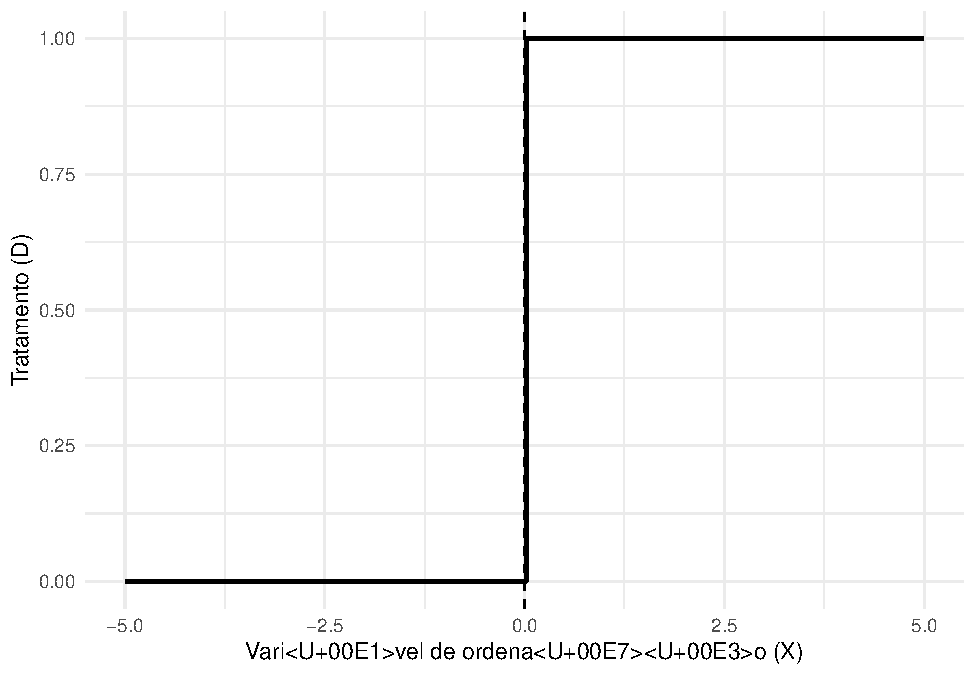
\includegraphics[alt={Gr<U+00E1>fico em degrau mostrando D igual a zero <U+00E0> esquerda do cutoff e igual a um <U+00E0> direita.}]{bookdownproj_files/figure-latex/plot-d-assignment-1} \caption{Regra sharp RD: o tratamento D muda mecanicamente no cutoff X = 0.}\label{fig:plot-d-assignment}
\end{figure}

Começamos olhando \(Y_i(0)\), o resultado que cada unidade teria sem tratamento.

\begin{figure}
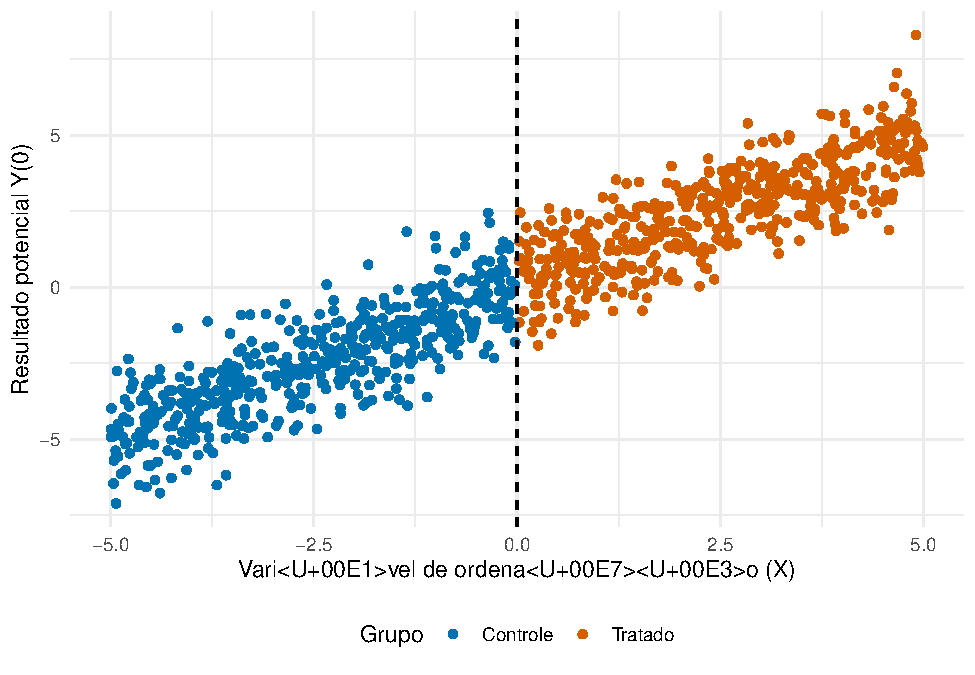
\includegraphics[alt={Dispers<U+00E3>o de Y(0) contra X sem salto vis<U+00ED>vel no cutoff.}]{bookdownproj_files/figure-latex/plot-po-y0-1} \caption{Resultado potencial sob controle: Y(0) varia suavemente ao redor do cutoff.}\label{fig:plot-po-y0}
\end{figure}

Agora olhamos \(Y_i(1)\), o resultado que cada unidade teria sob tratamento.

\begin{figure}
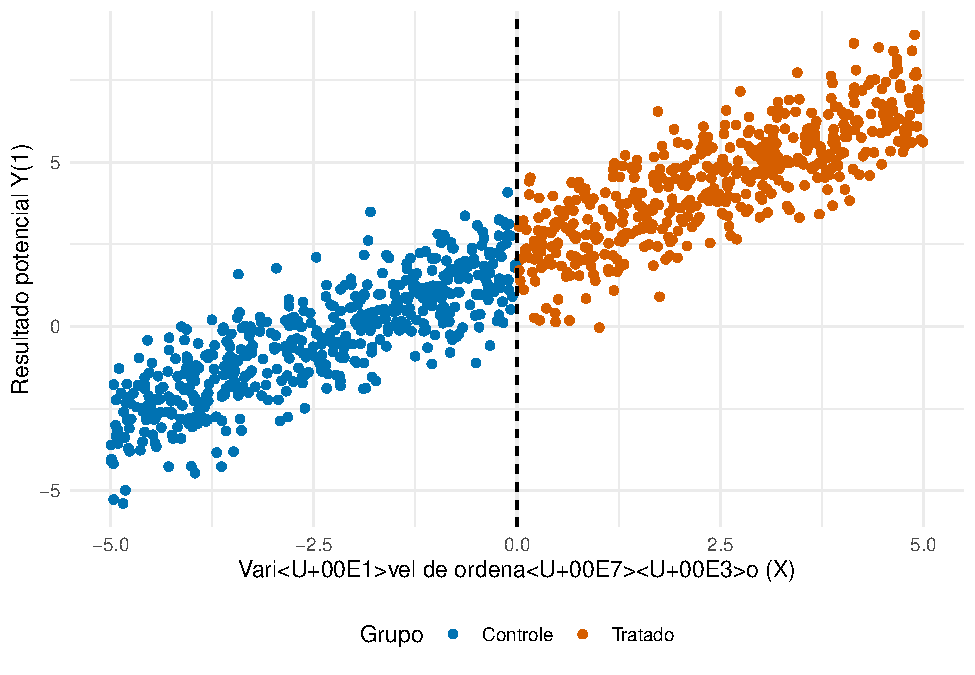
\includegraphics[alt={Dispers<U+00E3>o de Y(1) contra X sem salto abrupto no cutoff.}]{bookdownproj_files/figure-latex/plot-po-y1-1} \caption{Resultado potencial sob tratamento: Y(1) tamb<U+00E9>m <U+00E9> suave no cutoff.}\label{fig:plot-po-y1}
\end{figure}

Colocar \(Y_i(0)\) e \(Y_i(1)\) no mesmo gráfico mostra a lógica do desenho: os resultados potenciais são suaves, mas só observamos um deles para cada unidade.

\begin{figure}
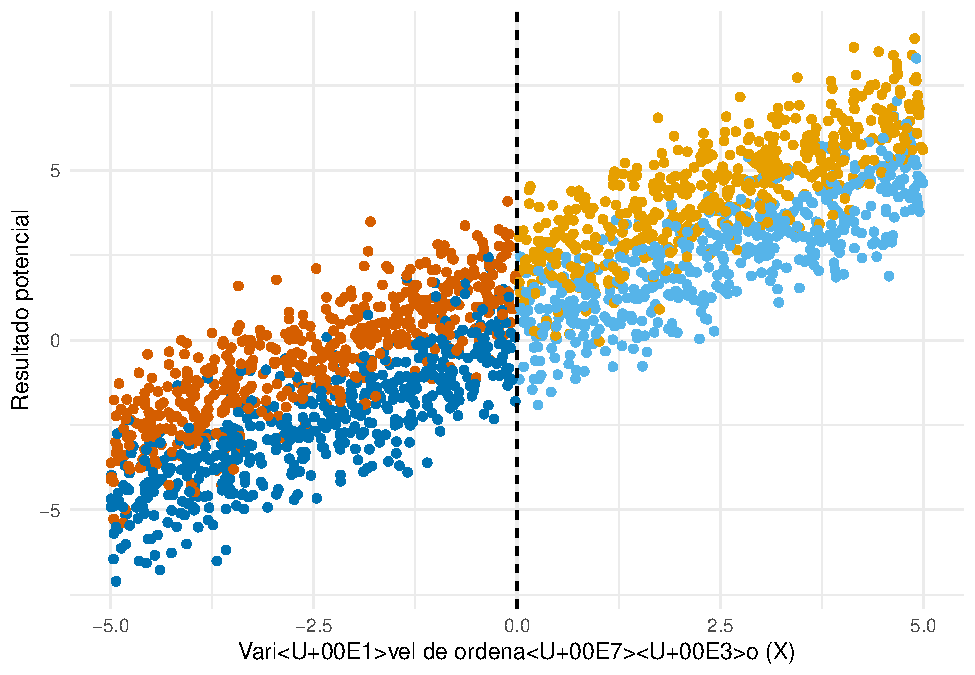
\includegraphics[alt={Dispers<U+00E3>o dos resultados potenciais Y(0) e Y(1) por lado do cutoff.}]{bookdownproj_files/figure-latex/plot-po-y1-Y0-1} \caption{Resultados potenciais simulados por status de tratamento observado.}\label{fig:plot-po-y1-Y0-1}
\end{figure}
\begin{figure}
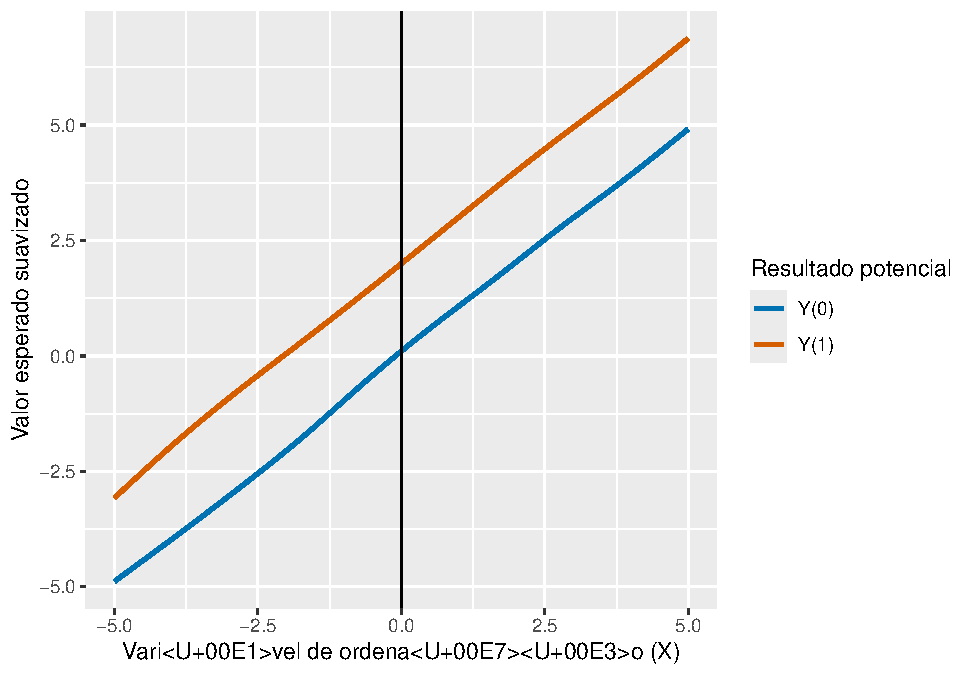
\includegraphics[alt={Curvas suavizadas de Y(0) e Y(1) contra X, ambas cont<U+00ED>nuas no cutoff.}]{bookdownproj_files/figure-latex/plot-po-y1-Y0-2} \caption{Fun<U+00E7><U+00F5>es suavizadas de Y(0) e Y(1): o efeito de RD vem do salto no tratamento, n<U+00E3>o de uma quebra nos resultados potenciais.}\label{fig:plot-po-y1-Y0-2}
\end{figure}

O resultado observado combina esses dois resultados potenciais de acordo com a regra de tratamento.

\begin{figure}
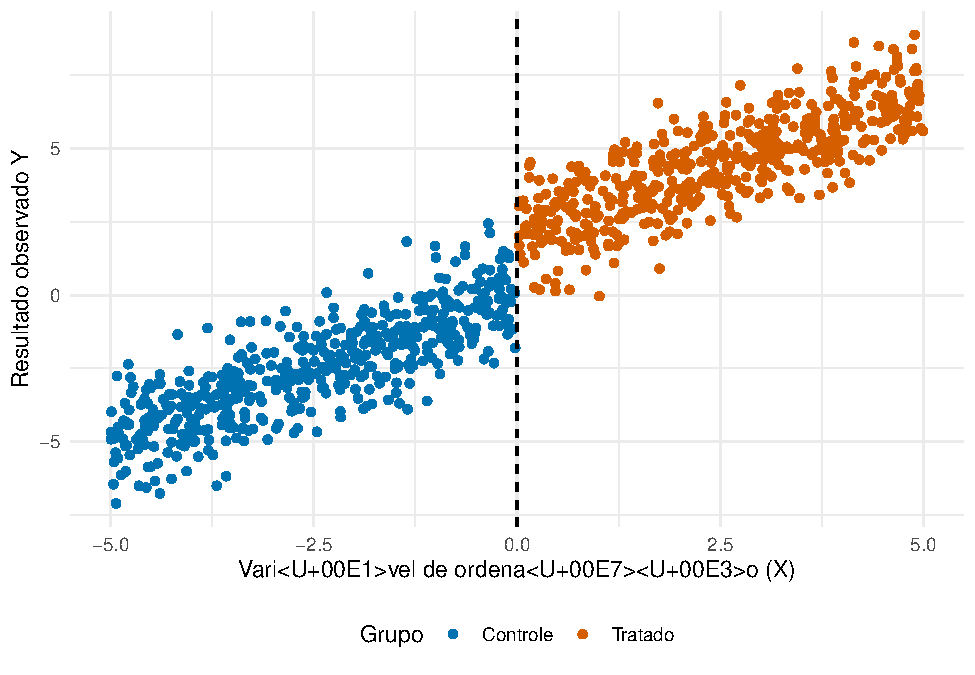
\includegraphics[alt={Dispers<U+00E3>o do resultado observado contra X com mudan<U+00E7>a de n<U+00ED>vel no cutoff.}]{bookdownproj_files/figure-latex/plot-observed-1} \caption{Resultado observado: o salto em Y aparece porque o tratamento muda no cutoff.}\label{fig:plot-observed}
\end{figure}

A simulação acima ilustra os elementos fundamentais de um RDD. Vejamos agora em que condições as estimativas de RDD são válidas.

\subsection{Quando o RDD funciona?}\label{quando-o-rdd-funciona}

A suposição chave para o RDD não é que o resultado salte no cutoff. O resultado pode não saltar se o efeito causal for zero. O que precisa saltar é o tratamento, ou a probabilidade de tratamento no caso fuzzy. Para que o salto no resultado possa ser interpretado causalmente, os resultados potenciais e covariáveis de pré-tratamento devem variar suavemente ao redor do cutoff. Vamos ver o que isso significa comparando cinco gráficos: alguns em que a estimativa de RD é válida, ainda que com diferentes graus de validade externa, e um em que a descontinuidade em outra variável torna o desenho inválido.

\begin{figure}
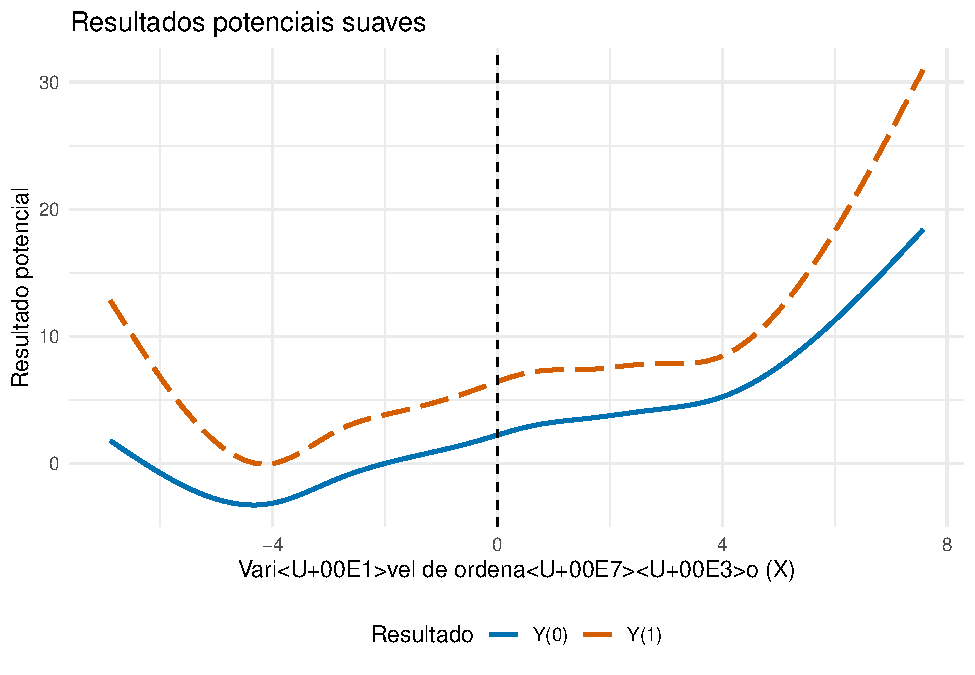
\includegraphics[alt={Curvas suavizadas de Y(0) e Y(1) sem quebra no cutoff.}]{bookdownproj_files/figure-latex/caso-rdd-suave-1} \caption{Caso 1: resultados potenciais suaves e salto claro no tratamento.}\label{fig:caso-rdd-suave}
\end{figure}

\begin{figure}
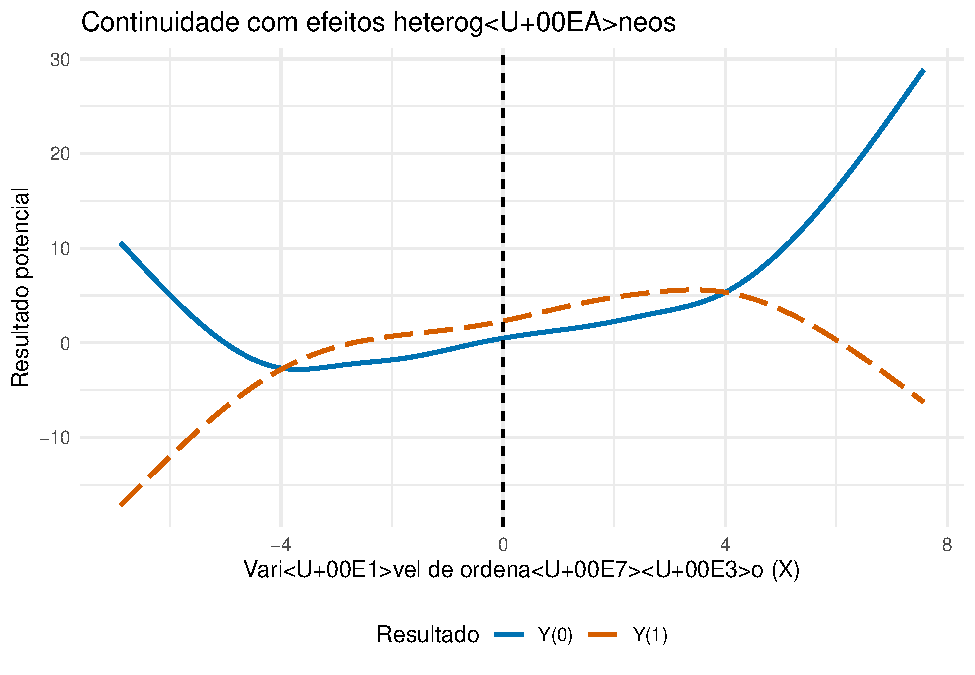
\includegraphics[alt={Curvas de resultados potenciais com heterogeneidade e continuidade em zero.}]{bookdownproj_files/figure-latex/caso-rdd-heterogeneo-1} \caption{Caso 2: efeitos heterog<U+00EA>neos, mas resultados potenciais ainda suaves no cutoff.}\label{fig:caso-rdd-heterogeneo}
\end{figure}

\begin{figure}
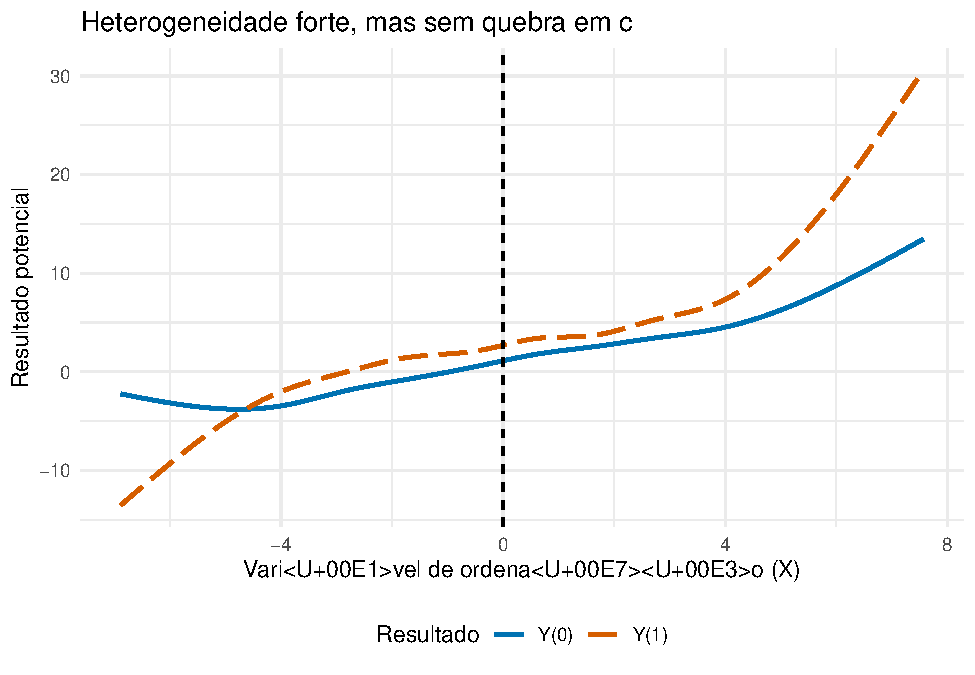
\includegraphics[alt={Curvas de resultados potenciais com heterogeneidade forte e continuidade no cutoff.}]{bookdownproj_files/figure-latex/caso-rdd-heterogeneo-forte-1} \caption{Caso 3: heterogeneidade mais forte, com continuidade preservada no cutoff.}\label{fig:caso-rdd-heterogeneo-forte}
\end{figure}

\begin{figure}
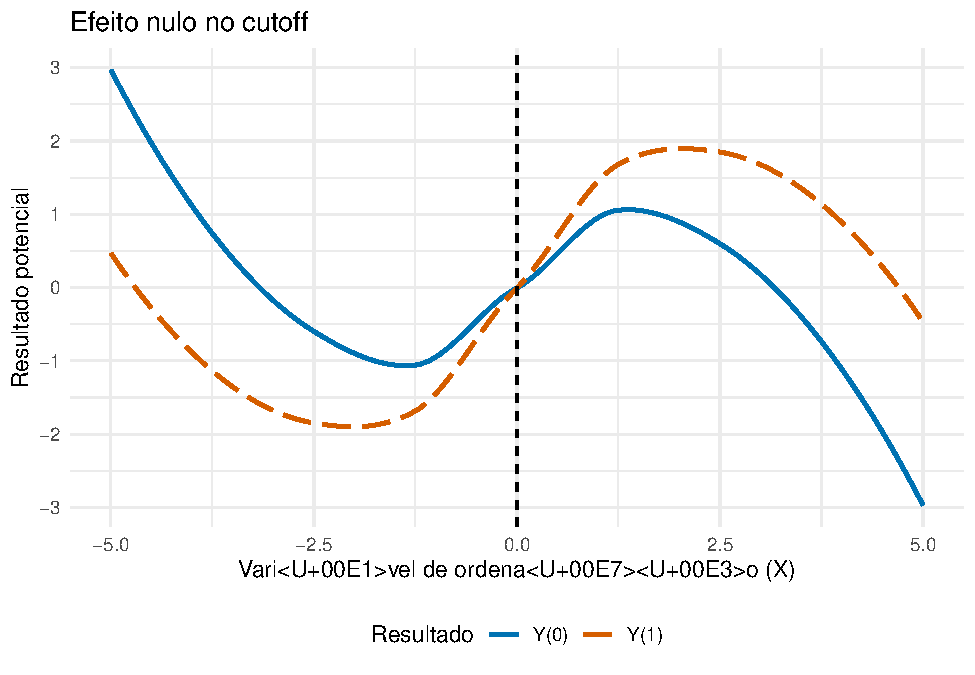
\includegraphics[alt={Curvas de Y(0) e Y(1) que se encontram no cutoff.}]{bookdownproj_files/figure-latex/caso-rdd-efeito-nulo-1} \caption{Caso 4: nenhum efeito exatamente no cutoff, apesar de as fun<U+00E7><U+00F5>es diferirem longe dele.}\label{fig:caso-rdd-efeito-nulo}
\end{figure}

\begin{figure}
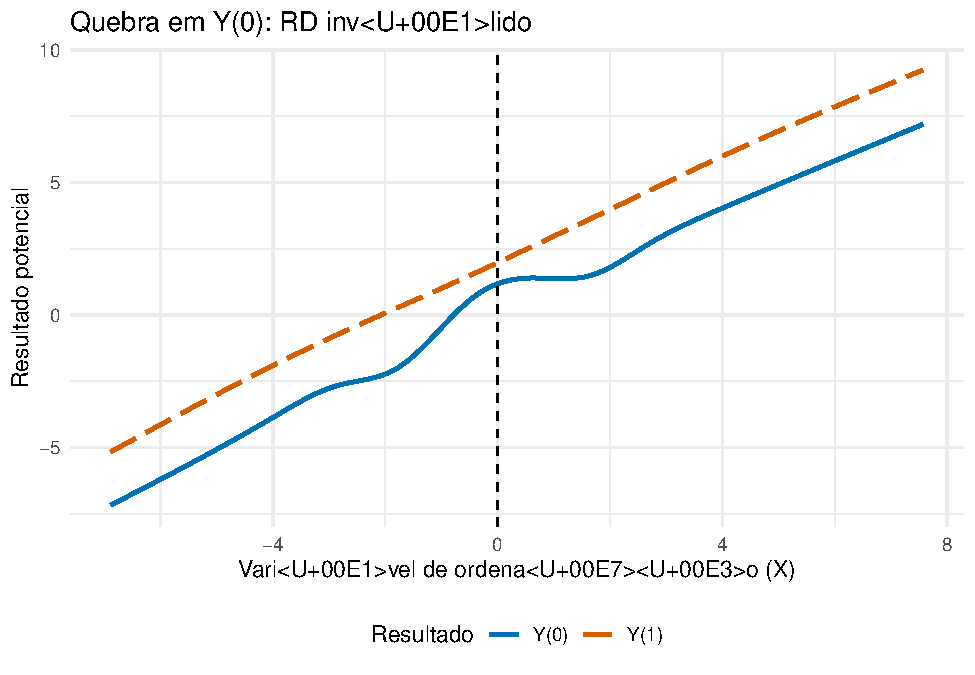
\includegraphics[alt={Curva de Y(0) com salto artificial ao redor do cutoff, invalidando o desenho.}]{bookdownproj_files/figure-latex/caso-rdd-invalido-1} \caption{Caso 5: desenho inv<U+00E1>lido, pois Y(0) apresenta uma descontinuidade no cutoff.}\label{fig:caso-rdd-invalido}
\end{figure}

Os quatro primeiros casos preservam a continuidade dos resultados potenciais no cutoff. Eles diferem em heterogeneidade e validade externa, mas a comparação local continua interpretável. O quinto caso quebra a lógica do desenho: mesmo sem tratamento, \(Y_i(0)\) mudaria abruptamente em \(c\).

\subsection{Dados brutos versus bins}\label{dados-brutos-versus-bins}

\begin{figure}
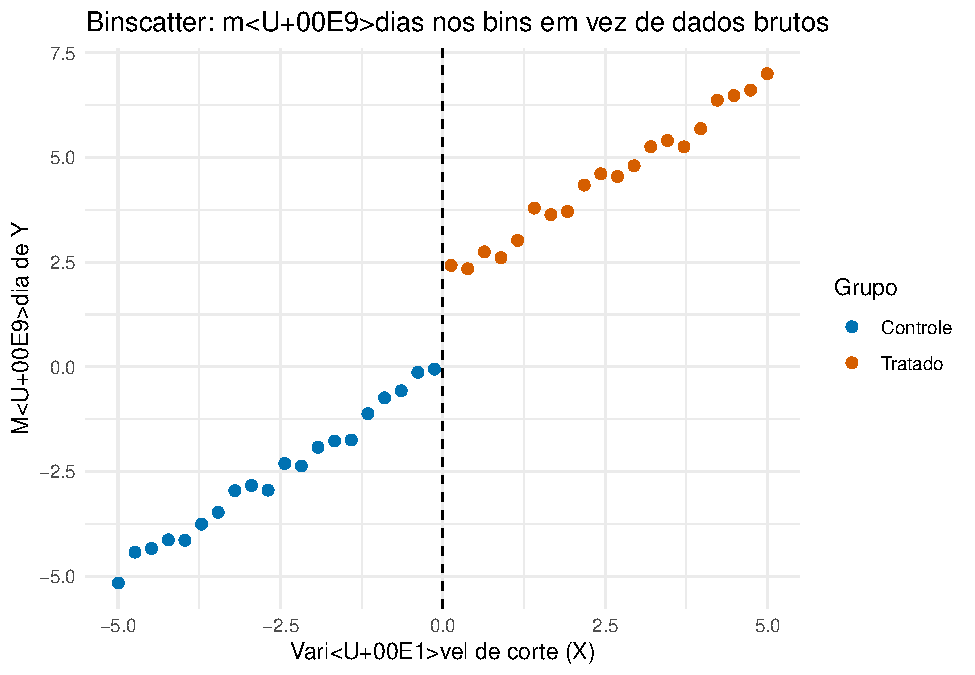
\includegraphics[alt={Gr<U+00E1>fico de m<U+00E9>dias de Y por bins igualmente espa<U+00E7>ados da running variable.}]{bookdownproj_files/figure-latex/plot-binscatter-1} \caption{Binscatter com bins igualmente espa<U+00E7>ados: os pontos mostram m<U+00E9>dias locais de Y.}\label{fig:plot-binscatter}
\end{figure}

Como escolher os bins?

\begin{enumerate}
\def\labelenumi{\arabic{enumi}.}
\tightlist
\item
  Espaçamentos iguais ou quantis?
\item
  Quantos bins?
\end{enumerate}

No exemplo, escolhi espaçamento igual e 20 bins. Podemos usar quantis.

\begin{figure}
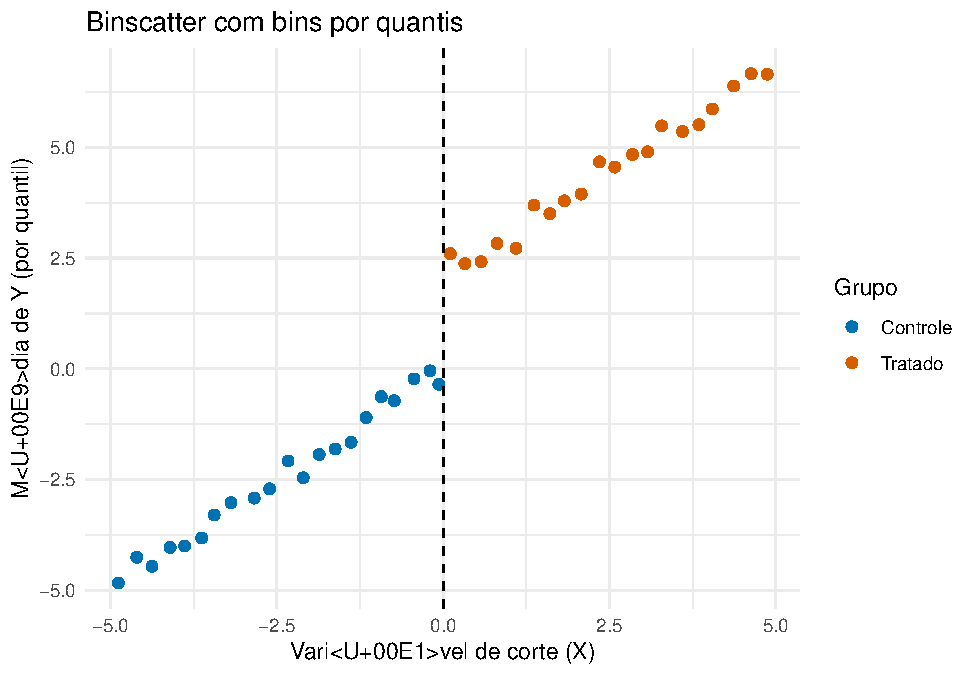
\includegraphics[alt={Gr<U+00E1>fico de m<U+00E9>dias de Y por bins definidos por quantis da running variable.}]{bookdownproj_files/figure-latex/plot-binscatter-quantis-1} \caption{Binscatter com bins por quantis: cada bin cont<U+00E9>m n<U+00FA>mero semelhante de observa<U+00E7><U+00F5>es.}\label{fig:plot-binscatter-quantis}
\end{figure}

Esses gráficos servem para visualização, não para estimação. A escolha dos bins afeta como a evidência aparece no gráfico, mas a estimativa principal deve vir da regressão local com bandwidth explícito. Bins por quantis ajudam a evitar bins vazios e tornam os pontos visualmente mais estáveis, mas também podem esconder variações na densidade da \emph{running variable}. Por isso, o gráfico de RD deve ser acompanhado por diagnósticos de densidade.

Sobre o número de bins, Cattaneo et al.~(2020) discutem duas abordagens. A primeira minimiza o IMSE, \emph{Integrated Mean Squared Error}, isto é, o erro quadrático médio integrado ao longo da função estimada. A segunda busca imitar a variância da nuvem de pontos original, o que costuma produzir mais bins.

O pacote \texttt{rdplot} implementa essas escolhas automaticamente.

\begin{figure}
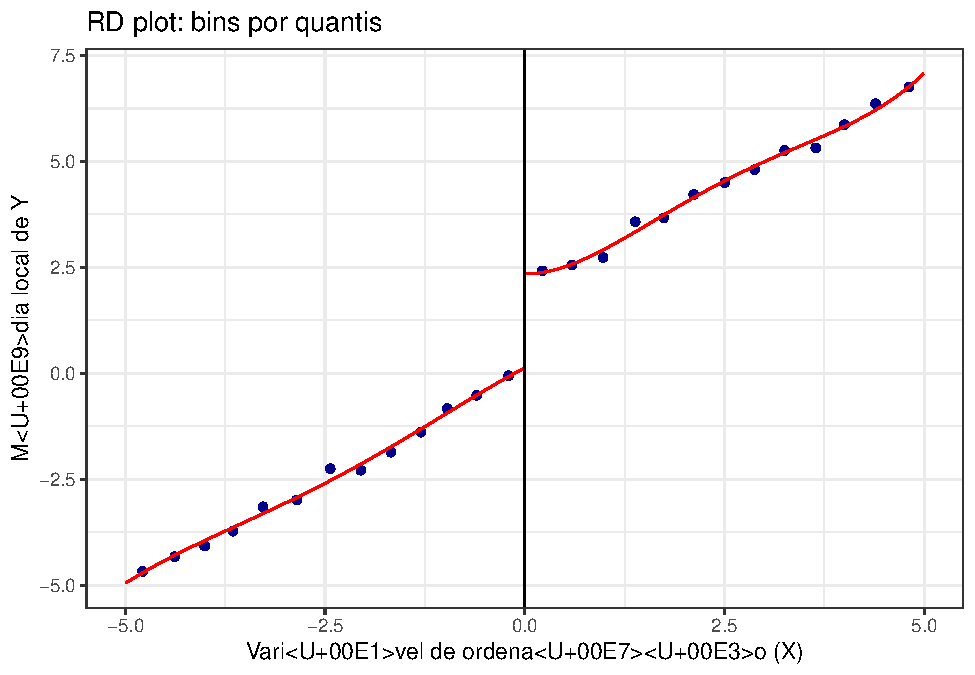
\includegraphics[alt={RD plot com pontos por bins e ajuste local nos dois lados do cutoff.}]{bookdownproj_files/figure-latex/plot-binscatter-quantis-rdplot-qs-1} \caption{RD plot com sele<U+00E7><U+00E3>o autom<U+00E1>tica de bins por quantis.}\label{fig:plot-binscatter-quantis-rdplot-qs}
\end{figure}

\begin{figure}
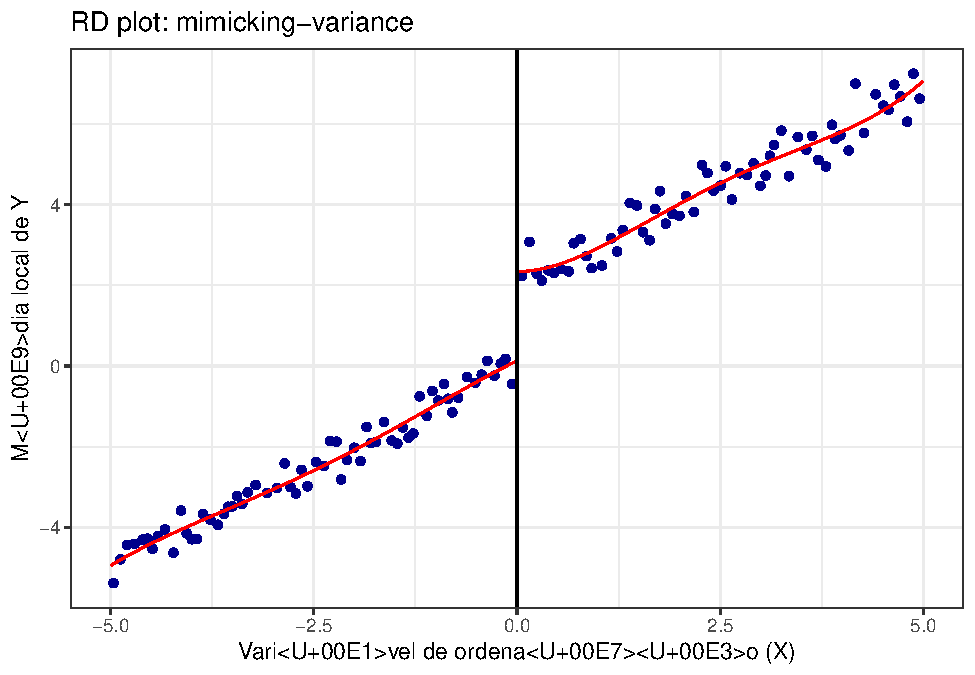
\includegraphics[alt={RD plot com bins definidos para aproximar a vari<U+00E2>ncia visual dos dados brutos.}]{bookdownproj_files/figure-latex/plot-binscatter-quantis-rdplot-qsmv-1} \caption{RD plot com sele<U+00E7><U+00E3>o de bins mimicking-variance.}\label{fig:plot-binscatter-quantis-rdplot-qsmv}
\end{figure}

\subsection{Testes de permutação para balanceamento}\label{testes-de-permutauxe7uxe3o-para-balanceamento}

Para checar balanceamento, podemos usar testes de permutação em covariáveis pré-tratamento. No exemplo abaixo, \texttt{w\_pre} representa uma covariável observável medida antes do tratamento. O teste pergunta se sua distribuição muda de forma anormal no cutoff.

\begin{Shaded}
\begin{Highlighting}[]
\FunctionTok{library}\NormalTok{(RATest)}
\NormalTok{df\_perm }\OtherTok{\textless{}{-}}\NormalTok{ df\_u}
\NormalTok{resultado }\OtherTok{\textless{}{-}} \FunctionTok{RDperm}\NormalTok{(}
  \AttributeTok{W =} \StringTok{"w\_pre"}\NormalTok{,}
  \AttributeTok{z =} \StringTok{"x"}\NormalTok{,}
  \AttributeTok{data =}\NormalTok{ df\_perm,}
  \AttributeTok{cutoff =} \DecValTok{0}
\NormalTok{)}

\NormalTok{df\_perm }\SpecialCharTok{\%\textgreater{}\%}
  \FunctionTok{mutate}\NormalTok{(}\AttributeTok{lado =} \FunctionTok{ifelse}\NormalTok{(x }\SpecialCharTok{\textless{}} \DecValTok{0}\NormalTok{, }\StringTok{"À esquerda do cutoff"}\NormalTok{, }\StringTok{"À direita do cutoff"}\NormalTok{)) }\SpecialCharTok{\%\textgreater{}\%}
  \FunctionTok{ggplot}\NormalTok{(}\FunctionTok{aes}\NormalTok{(}\AttributeTok{x =}\NormalTok{ w\_pre, }\AttributeTok{colour =}\NormalTok{ lado, }\AttributeTok{linetype =}\NormalTok{ lado)) }\SpecialCharTok{+}
  \FunctionTok{stat\_ecdf}\NormalTok{(}\AttributeTok{linewidth =} \FloatTok{0.9}\NormalTok{) }\SpecialCharTok{+}
  \FunctionTok{scale\_colour\_manual}\NormalTok{(}\AttributeTok{values =} \FunctionTok{c}\NormalTok{(}\StringTok{"À esquerda do cutoff"} \OtherTok{=} \StringTok{"\#0072B2"}\NormalTok{, }\StringTok{"À direita do cutoff"} \OtherTok{=} \StringTok{"\#D55E00"}\NormalTok{)) }\SpecialCharTok{+}
  \FunctionTok{scale\_linetype\_manual}\NormalTok{(}\AttributeTok{values =} \FunctionTok{c}\NormalTok{(}\StringTok{"À esquerda do cutoff"} \OtherTok{=} \StringTok{"solid"}\NormalTok{, }\StringTok{"À direita do cutoff"} \OtherTok{=} \StringTok{"longdash"}\NormalTok{)) }\SpecialCharTok{+}
  \FunctionTok{labs}\NormalTok{(}
    \AttributeTok{x =} \StringTok{"Covariável pré{-}tratamento"}\NormalTok{,}
    \AttributeTok{y =} \StringTok{"Distribuição acumulada empírica"}\NormalTok{,}
    \AttributeTok{colour =} \StringTok{"Lado"}\NormalTok{,}
    \AttributeTok{linetype =} \StringTok{"Lado"}
\NormalTok{  ) }\SpecialCharTok{+}
  \FunctionTok{theme\_minimal}\NormalTok{() }\SpecialCharTok{+}
  \FunctionTok{theme}\NormalTok{(}\AttributeTok{legend.position =} \StringTok{"bottom"}\NormalTok{)}
\end{Highlighting}
\end{Shaded}

\begin{figure}
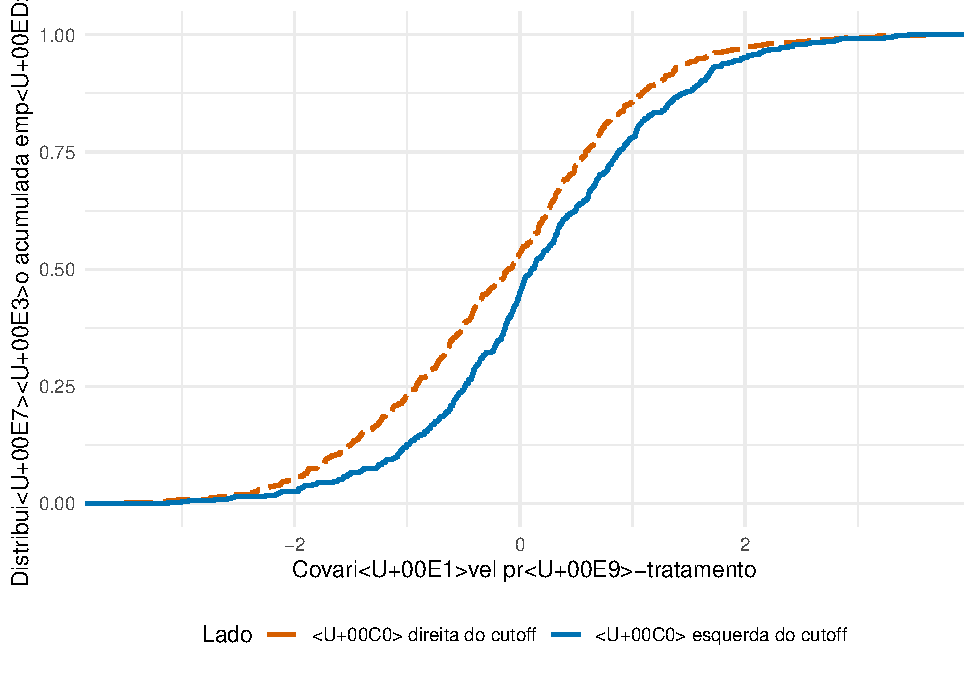
\includegraphics[alt={Fun<U+00E7><U+00F5>es de distribui<U+00E7><U+00E3>o acumulada emp<U+00ED>ricas de uma covari<U+00E1>vel pr<U+00E9>-tratamento <U+00E0> esquerda e <U+00E0> direita do cutoff.}]{bookdownproj_files/figure-latex/permutation-test-1} \caption{Teste de permuta<U+00E7><U+00E3>o para uma covari<U+00E1>vel pr<U+00E9>-tratamento observ<U+00E1>vel.}\label{fig:permutation-test}
\end{figure}

Canay \& Kamat (2018) utilizaram esse teste para revisitar o trabalho de Lee (2008) e descobriram que havia problema de balanceamento.

Caughey and Sekhon (2011) na political analysis mostraram que de fato havia problemas de balanceamento no estudo de Lee (2008).

Testes de permutação são mais naturais no framework de aleatorização local. Eles exigem que o pesquisador escolha uma janela em que a atribuição ao tratamento seja plausivelmente ``como se aleatória''. Essa janela não deve ser simplesmente o bandwidth MSE/CER-optimal de \texttt{rdrobust}: bandwidths automáticos estimam limites laterais sob continuidade, enquanto a aleatorização local é uma afirmação mais forte sobre o mecanismo de atribuição dentro de uma janela.

Do artigo na \emph{Political Analysis}:

\begin{figure}
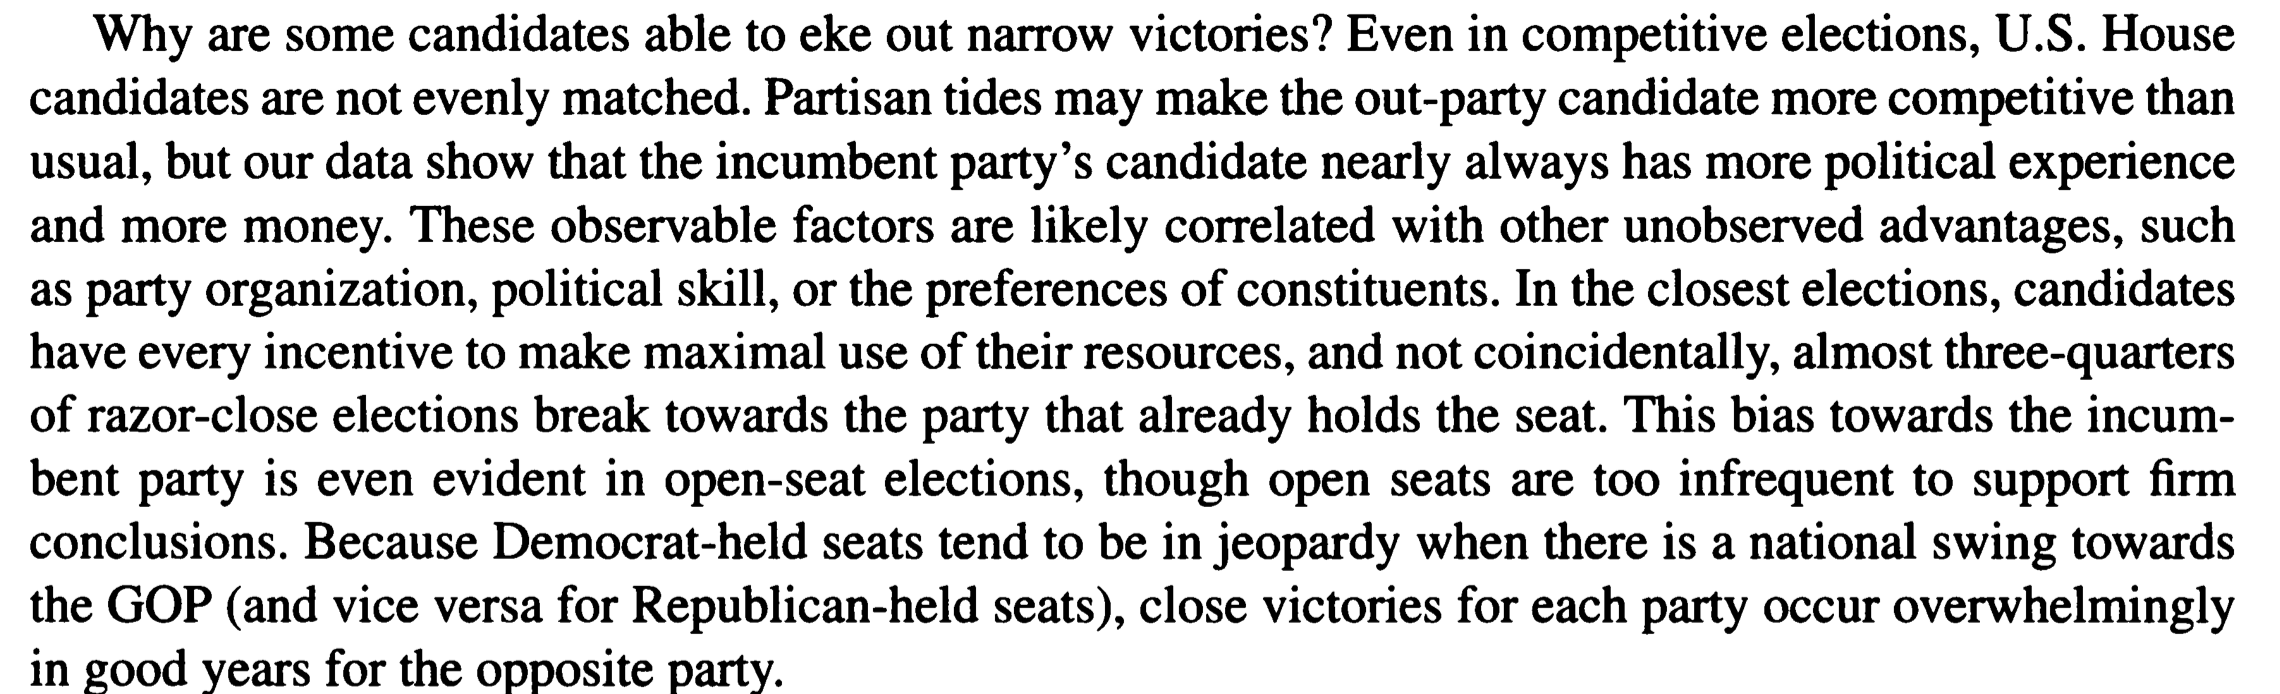
\includegraphics[width=0.9\linewidth,alt={Trecho do artigo de Caughey e Sekhon sobre problemas de balanceamento.}]{imagens/quote} \caption{Caughey e Sekhon (2011): alerta sobre balanceamento em elei<U+00E7><U+00F5>es apertadas.}\label{fig:quote-1}
\end{figure}
\begin{figure}
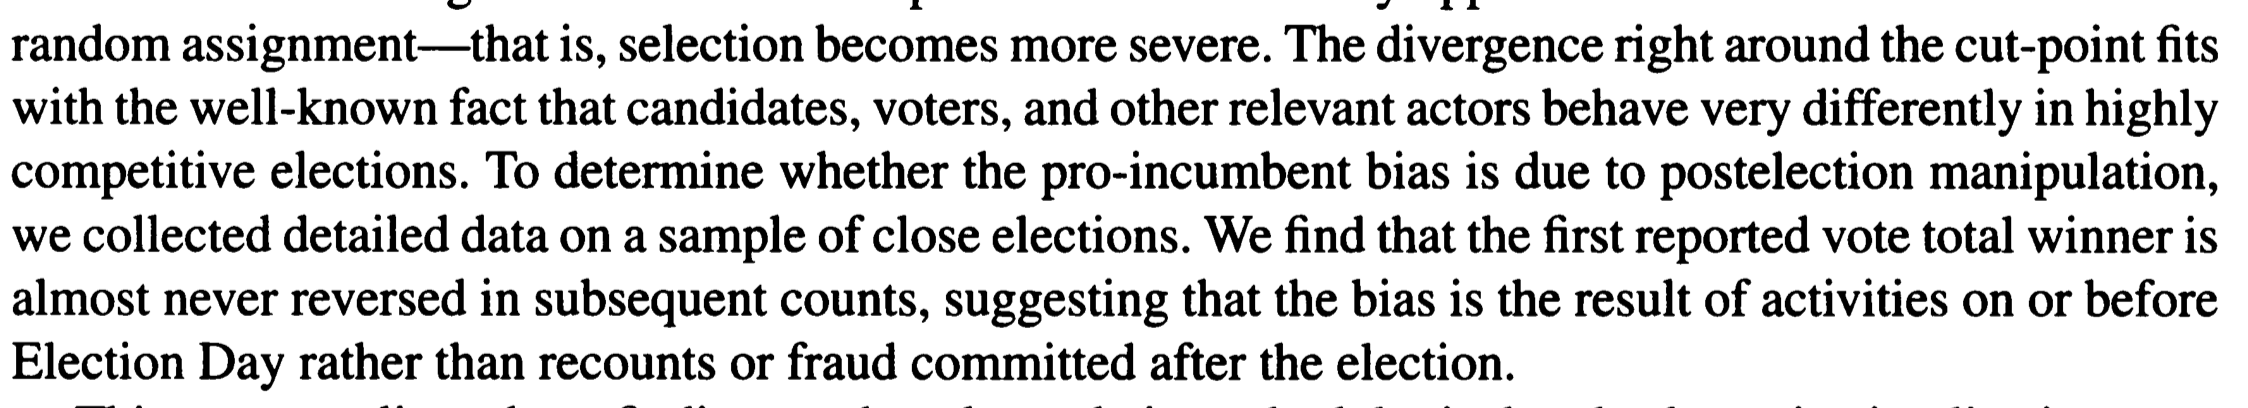
\includegraphics[width=0.9\linewidth,alt={Segundo trecho do artigo de Caughey e Sekhon sobre close elections.}]{imagens/quote2} \caption{Caughey e Sekhon (2011): implica<U+00E7><U+00E3>o para a interpreta<U+00E7><U+00E3>o de close elections.}\label{fig:quote-2}
\end{figure}

Houve um debate na ciência política sobre isso. Erikson \& Rader (2017) e Cuesta \& Imai (2016) argumentam que o RDD é identificado. Até onde eu sei, cientistas políticos não revisitaram a controvérsia com os novos métodos desenvolvidos pelos economistas.

De todo modo, as evidências de De Magalhães et al.~(2025) sugerem que a recomendação que estou adotando no curso de quais práticas usar são as melhores e mais robustas.

\subsection{Teste de McCrary e densidade}\label{teste-de-mccrary-e-densidade}

Um dos principais desafios à identificação causal em RDDs é a possibilidade de manipulação por parte dos agentes sobre ficar acima ou abaixo do ponto de corte. A lógica esperada é que se o tratamento é desejável, indivíduos tentarão receber o tratamento, levando a um gap justamente abaixo do ponto de corte. Se o tratamento é indesejável (efeitos negativos), indivíduos vão evitar o tratamento, levando a um gap justamente acima do ponto de corte.

O exemplo mais evidente para nós cientistas políticos é a aprovação de um projeto de lei no legislativo. Nós sabemos que os legisladores agem estrategicamente retirando propostas que não vão ser aprovadas ou postergando a votação, até terem a maioria, ainda que por margem mínima. Nesse caso, a aplicação de RDD produzirá estimativas viesadas. McCrary, em um artigo de 2008, argumentou que tais casos apareceriam como descontinuidade na densidade da \emph{running variable} ao redor do ponto de corte. Eis o gráfico feito por McCrary em seu estudo original:

\begin{figure}
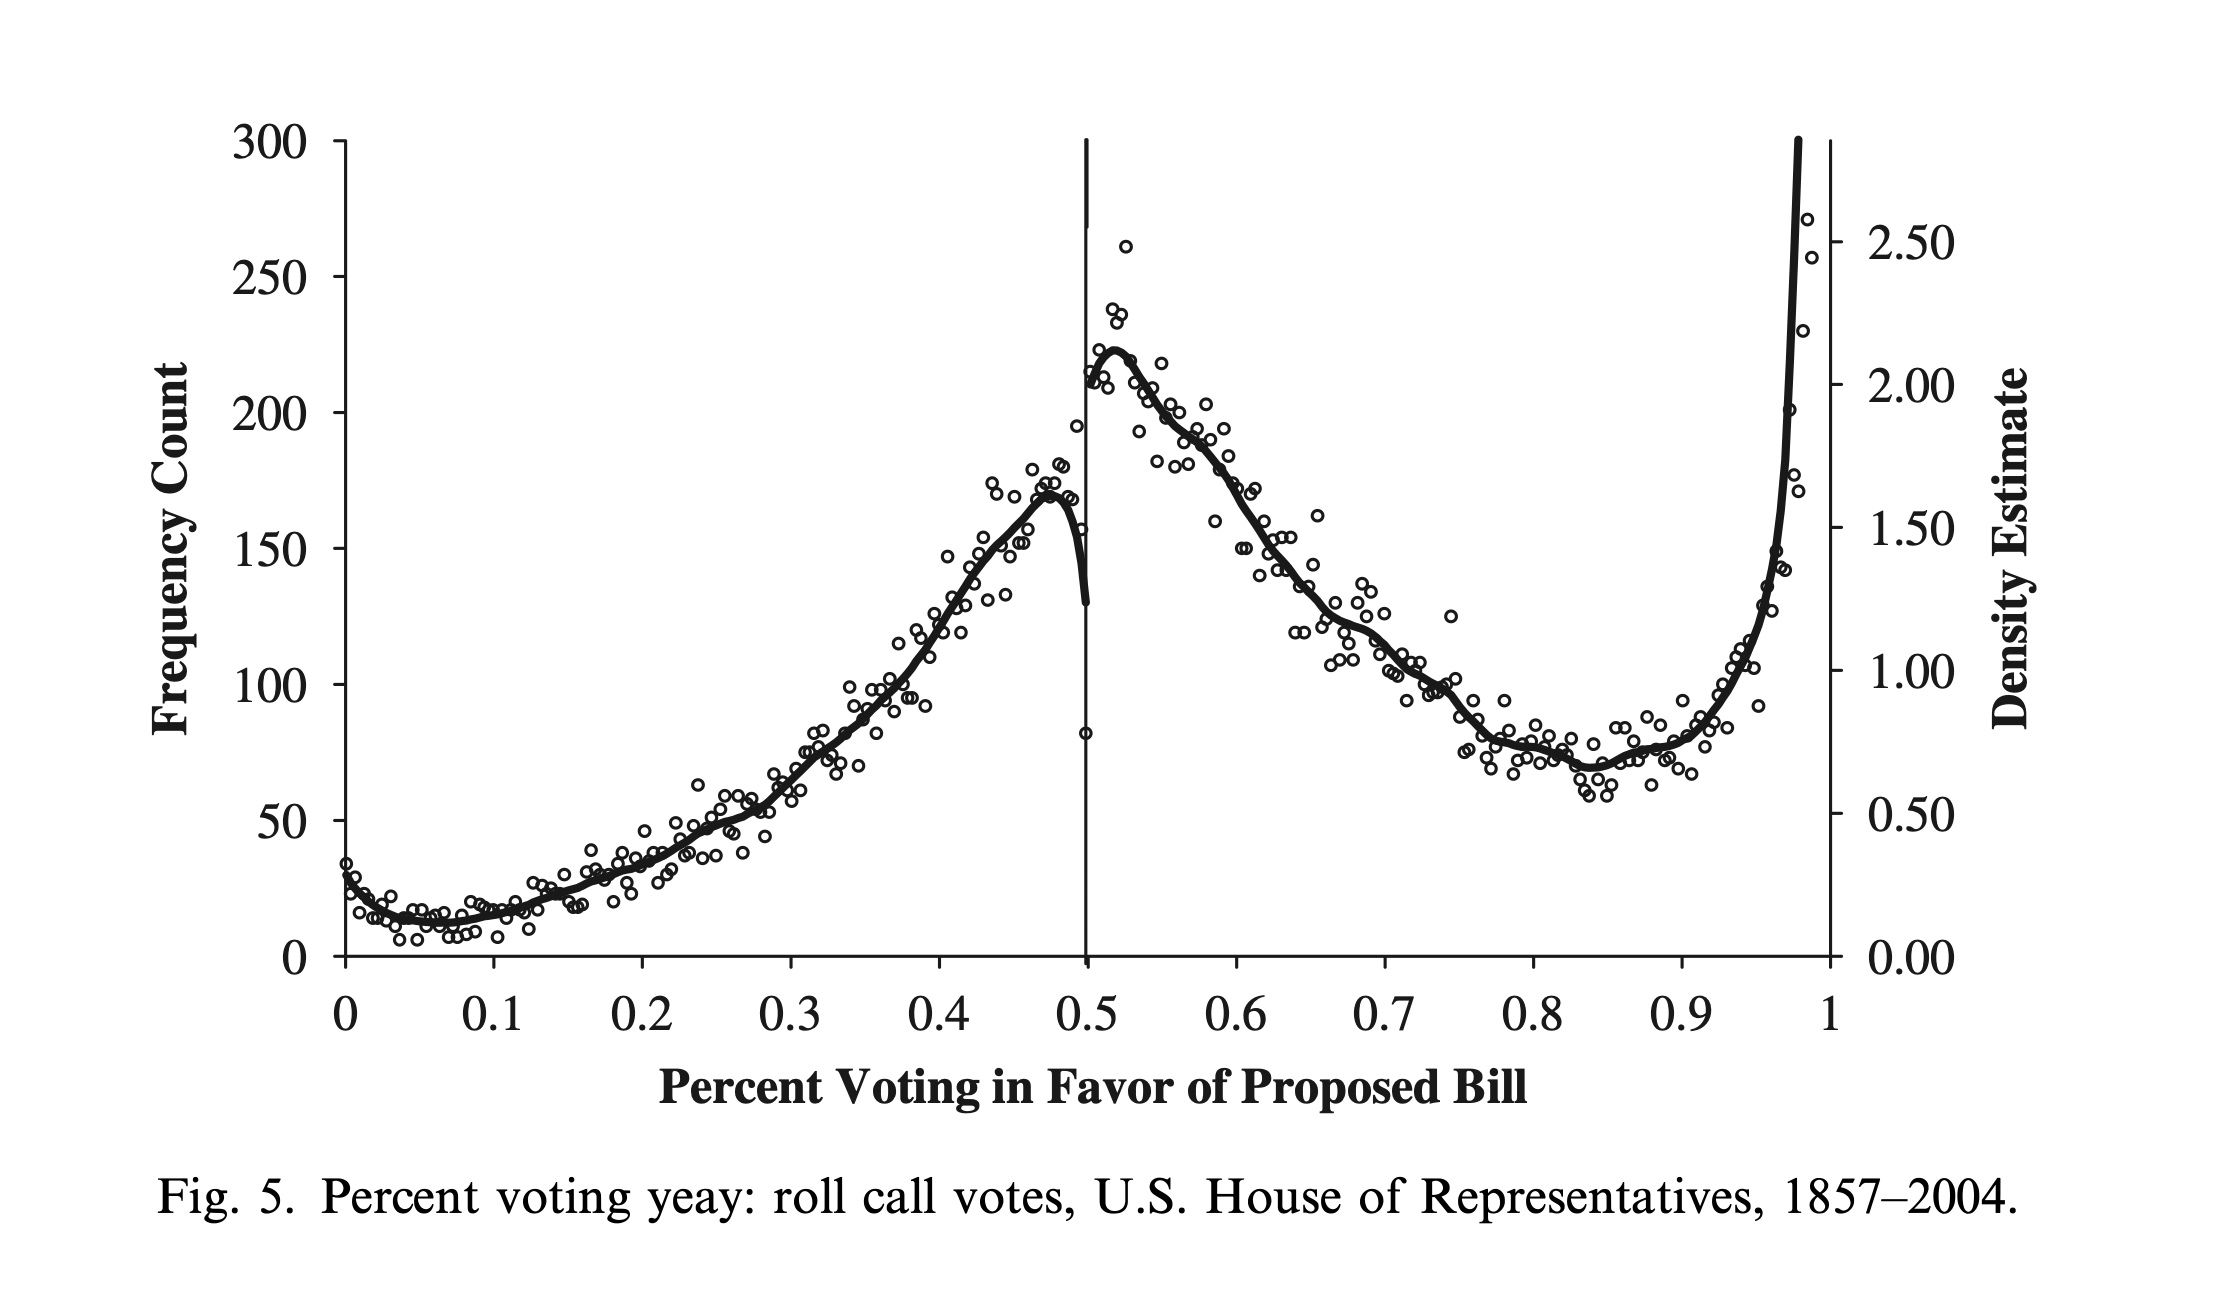
\includegraphics[width=30.75in,alt={Histograma e densidades laterais indicando poss<U+00ED>vel descontinuidade na densidade da running variable.}]{imagens/manipulation test} \caption{Figura cl<U+00E1>ssica do teste de manipula<U+00E7><U+00E3>o em McCrary (2008).}\label{fig:McCay-test}
\end{figure}

Para formalizar essa ideia, McCrary estima os limites da densidade pela esquerda e pela direita e avalia se a diferença (do logaritmo) das estimativas é estatisticamente significante diferente de zero. Portanto, rejeitar a hipótese nula é encontrar evidências de que há manipulação. Cattaneo, Jansson e Ma (2018, 2020) introduziram uma versão alternativa do teste, com espírito similar.

Na prática, de um ponto de vista retórico, o que pesquisadores querem é falhar em rejeitar a nula. Como o teste pode ter baixo poder, ausência de evidência não quer dizer evidência de ausência. Hartman (2021) e Fitzgerald (2025) defendem uma leitura mais exigente: em vez de apenas perguntar se rejeitamos manipulação, deveríamos perguntar se os dados permitem descartar manipulação substantivamente relevante. Isso leva a testes de equivalência, em que o pesquisador define uma margem de manipulação considerada pequena o bastante para não comprometer o desenho.

\begin{figure}
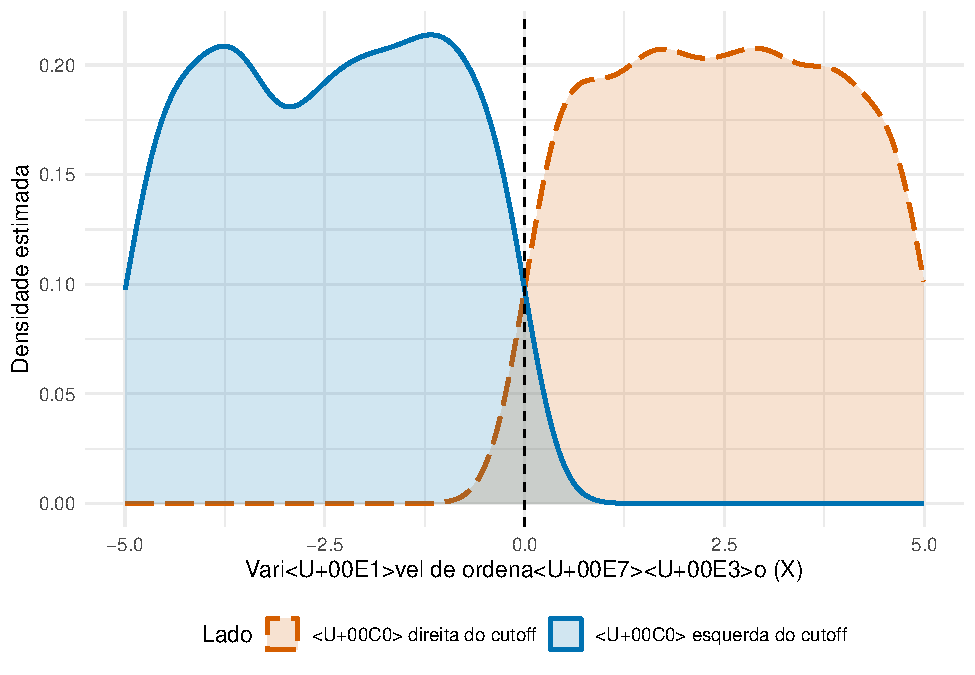
\includegraphics[alt={Densidades estimadas da vari<U+00E1>vel de ordena<U+00E7><U+00E3>o <U+00E0> esquerda e <U+00E0> direita do cutoff.}]{bookdownproj_files/figure-latex/McCay-test1-1} \caption{Diagn<U+00F3>stico visual de densidade: n<U+00E3>o h<U+00E1> ac<U+00FA>mulo evidente de observa<U+00E7><U+00F5>es no cutoff.}\label{fig:McCay-test1}
\end{figure}

Uma implementação mais moderna é o teste de densidade de Cattaneo, Jansson e Ma. A tabela resume o diagnóstico em vez de despejar todo o output do pacote.

\begin{table}

\caption{\label{tab:Cattaneo-test}Teste de densidade de Cattaneo, Jansson e Ma para os dados simulados.}
\centering
\begin{tabular}[t]{l|r}
\hline
Medida & Valor\\
\hline
Diferen<U+00E7>a estimada na densidade & 0.011\\
\hline
Estat<U+00ED>stica t & 0.279\\
\hline
p-valor & 0.780\\
\hline
\end{tabular}
\end{table}

Na Tabela \ref{tab:Cattaneo-test}, a hipótese nula é continuidade da densidade de \(X_i\) no cutoff. A diferença estimada na densidade é 0.011, isto é, praticamente zero neste exemplo. A estatística \(t\) é 0.279 e o p-valor é 0.78. Como o p-valor é alto, não rejeitamos a hipótese nula de continuidade da densidade. A interpretação substantiva é que, nesses dados simulados, não há evidência de acúmulo ou buraco de observações exatamente no cutoff. Isso não prova ausência de manipulação; apenas indica que o diagnóstico não encontrou uma descontinuidade detectável na densidade.

Essa é uma área ativa de pesquisa. Para a aula, o ponto é simples: \texttt{rddensity} é um diagnóstico útil, mas não substitui conhecimento institucional sobre quem poderia manipular \(X\), com que precisão e em que direção.

\subsection{Robustez e inferência em R}\label{robustez-e-inferuxeancia-em-r}

A análise aplicada deve separar três objetos: o gráfico, a estimativa e a inferência. O gráfico ajuda a avaliar a plausibilidade da descontinuidade. A estimativa vem da regressão local. A inferência moderna deve usar os intervalos robustos com correção de viés de \texttt{rdrobust}, não apenas o erro padrão convencional.

\begin{Shaded}
\begin{Highlighting}[]
\FunctionTok{library}\NormalTok{(rdrobust)}

\NormalTok{df }\OtherTok{\textless{}{-}}\NormalTok{ df\_aux}

\CommentTok{\# Estimativa sharp RD com bandwidth MSE{-}optimal.}
\NormalTok{modelo\_mse }\OtherTok{\textless{}{-}} \FunctionTok{rdrobust}\NormalTok{(}\AttributeTok{y =}\NormalTok{ df}\SpecialCharTok{$}\NormalTok{y, }\AttributeTok{x =}\NormalTok{ df}\SpecialCharTok{$}\NormalTok{x, }\AttributeTok{c =} \DecValTok{0}\NormalTok{, }\AttributeTok{p =} \DecValTok{1}\NormalTok{, }\AttributeTok{bwselect =} \StringTok{"mserd"}\NormalTok{)}

\CommentTok{\# Mesmo desenho, mas com bandwidth CER{-}optimal.}
\NormalTok{modelo\_cer }\OtherTok{\textless{}{-}} \FunctionTok{rdrobust}\NormalTok{(}\AttributeTok{y =}\NormalTok{ df}\SpecialCharTok{$}\NormalTok{y, }\AttributeTok{x =}\NormalTok{ df}\SpecialCharTok{$}\NormalTok{x, }\AttributeTok{c =} \DecValTok{0}\NormalTok{, }\AttributeTok{p =} \DecValTok{1}\NormalTok{, }\AttributeTok{bwselect =} \StringTok{"cerrd"}\NormalTok{)}
\end{Highlighting}
\end{Shaded}

No output de \texttt{rdrobust}, a linha Conventional usa a estimativa e o erro padrão convencionais. A linha Bias-Corrected corrige a estimativa pontual para viés. A linha Robust combina a estimativa corrigida com erro padrão apropriado para inferência robusta. Para reportar resultados principais, o padrão moderno é dar destaque ao intervalo robusto. A tabela abaixo mostra apenas os elementos que interessam para a aula.

\begin{table}

\caption{\label{tab:tabela-rdrobust}Estimativas sharp RD com infer<U+00EA>ncia robust bias-corrected.}
\centering
\begin{tabular}[t]{l|r|r|r|r|r}
\hline
Especifica<U+00E7><U+00E3>o & Estimativa & IC 95\% inferior & IC 95\% superior & h esquerda & h direita\\
\hline
MSE-optimal & 2.411 & 1.785 & 3.037 & 1.172 & 1.172\\
\hline
CER-optimal & 2.515 & 1.821 & 3.208 & 0.830 & 0.830\\
\hline
\end{tabular}
\end{table}

\begin{figure}
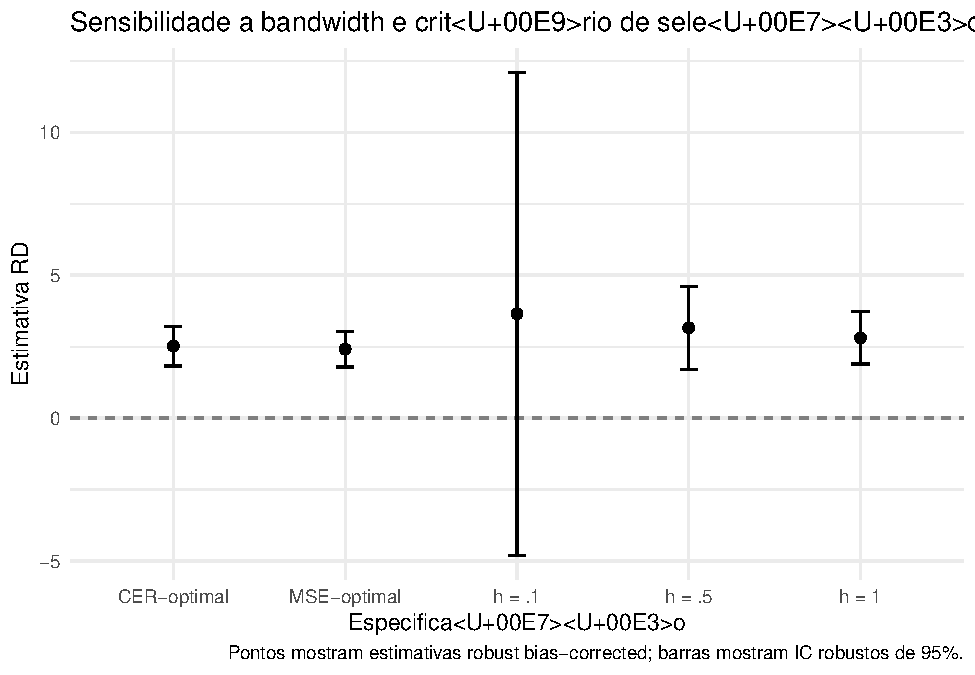
\includegraphics[alt={Gr<U+00E1>fico de pontos com intervalos de confian<U+00E7>a para especifica<U+00E7><U+00F5>es MSE, CER e bandwidths fixos.}]{bookdownproj_files/figure-latex/plot-efeitos-1} \caption{Sensibilidade da estimativa RD <U+00E0> escolha de bandwidth.}\label{fig:plot-efeitos}
\end{figure}

Esse gráfico é mais informativo do que uma sequência de gráficos separados porque coloca lado a lado a estimativa principal e alternativas razoáveis. Se a conclusão substantiva muda drasticamente com pequenas mudanças no bandwidth, o desenho precisa ser apresentado com mais cautela.

\subsubsection{Covariáveis em RD}\label{covariuxe1veis-em-rd}

Covariáveis de pré-tratamento podem melhorar precisão e ajudar nos diagnósticos, mas não salvam a identificação se a continuidade dos resultados potenciais for implausível. A literatura recente sobre covariáveis e aprendizado de máquina em RD reforça esse ponto: covariáveis devem ser vistas como ajuste de precisão e ferramenta de diagnóstico, não como substituto do desenho {[}Kreiß e Rothe 2023; Noack, Olma e Rothe 2025{]}.

\begin{Shaded}
\begin{Highlighting}[]
\FunctionTok{set.seed}\NormalTok{(}\DecValTok{1234}\NormalTok{)}
\NormalTok{df}\SpecialCharTok{$}\NormalTok{w\_pre }\OtherTok{\textless{}{-}} \FloatTok{0.3} \SpecialCharTok{*}\NormalTok{ df}\SpecialCharTok{$}\NormalTok{x }\SpecialCharTok{+} \FunctionTok{rnorm}\NormalTok{(}\FunctionTok{nrow}\NormalTok{(df))}

\NormalTok{modelo\_sem\_cov }\OtherTok{\textless{}{-}} \FunctionTok{rdrobust}\NormalTok{(}\AttributeTok{y =}\NormalTok{ df}\SpecialCharTok{$}\NormalTok{y, }\AttributeTok{x =}\NormalTok{ df}\SpecialCharTok{$}\NormalTok{x, }\AttributeTok{c =} \DecValTok{0}\NormalTok{, }\AttributeTok{p =} \DecValTok{1}\NormalTok{)}
\NormalTok{modelo\_com\_cov }\OtherTok{\textless{}{-}} \FunctionTok{rdrobust}\NormalTok{(}
  \AttributeTok{y =}\NormalTok{ df}\SpecialCharTok{$}\NormalTok{y,}
  \AttributeTok{x =}\NormalTok{ df}\SpecialCharTok{$}\NormalTok{x,}
  \AttributeTok{c =} \DecValTok{0}\NormalTok{,}
  \AttributeTok{p =} \DecValTok{1}\NormalTok{,}
  \AttributeTok{covs =} \FunctionTok{as.matrix}\NormalTok{(df}\SpecialCharTok{$}\NormalTok{w\_pre)}
\NormalTok{)}
\end{Highlighting}
\end{Shaded}

\begin{table}

\caption{\label{tab:tabela-rd-covs}Covari<U+00E1>veis pr<U+00E9>-tratamento podem mudar precis<U+00E3>o, mas n<U+00E3>o substituem a identifica<U+00E7><U+00E3>o.}
\centering
\begin{tabular}[t]{l|r|r|r|r|r}
\hline
especificacao & Estimativa & ic\_95\_inf & ic\_95\_sup & h\_esquerda & h\_direita\\
\hline
Sem covari<U+00E1>vel & 2.411 & 1.785 & 3.037 & 1.172 & 1.172\\
\hline
Com covari<U+00E1>vel pr<U+00E9>-tratamento & 2.432 & 1.790 & 3.075 & 1.077 & 1.077\\
\hline
\end{tabular}
\end{table}

\subsubsection{Fuzzy RD em R}\label{fuzzy-rd-em-r}

No fuzzy RD, o argumento \texttt{fuzzy} recebe a variável de tratamento efetivamente recebido. O pacote estima a razão entre o salto no resultado e o salto na probabilidade de tratamento.

\begin{Shaded}
\begin{Highlighting}[]
\FunctionTok{set.seed}\NormalTok{(}\DecValTok{4321}\NormalTok{)}
\NormalTok{prob\_tratamento }\OtherTok{\textless{}{-}} \FunctionTok{ifelse}\NormalTok{(df}\SpecialCharTok{$}\NormalTok{x }\SpecialCharTok{\textgreater{}=} \DecValTok{0}\NormalTok{, }\FloatTok{0.8}\NormalTok{, }\FloatTok{0.2}\NormalTok{)}
\NormalTok{d\_fuzzy }\OtherTok{\textless{}{-}} \FunctionTok{rbinom}\NormalTok{(}\FunctionTok{nrow}\NormalTok{(df), }\AttributeTok{size =} \DecValTok{1}\NormalTok{, }\AttributeTok{prob =}\NormalTok{ prob\_tratamento)}
\NormalTok{y\_fuzzy }\OtherTok{\textless{}{-}}\NormalTok{ df}\SpecialCharTok{$}\NormalTok{y0 }\SpecialCharTok{+} \DecValTok{2} \SpecialCharTok{*}\NormalTok{ d\_fuzzy }\SpecialCharTok{+} \FunctionTok{rnorm}\NormalTok{(}\FunctionTok{nrow}\NormalTok{(df), }\AttributeTok{sd =} \FloatTok{0.5}\NormalTok{)}

\NormalTok{modelo\_fuzzy }\OtherTok{\textless{}{-}} \FunctionTok{rdrobust}\NormalTok{(}
  \AttributeTok{y =}\NormalTok{ y\_fuzzy,}
  \AttributeTok{x =}\NormalTok{ df}\SpecialCharTok{$}\NormalTok{x,}
  \AttributeTok{c =} \DecValTok{0}\NormalTok{,}
  \AttributeTok{fuzzy =}\NormalTok{ d\_fuzzy}
\NormalTok{)}

\NormalTok{modelo\_rf\_fuzzy }\OtherTok{\textless{}{-}} \FunctionTok{rdrobust}\NormalTok{(}\AttributeTok{y =}\NormalTok{ y\_fuzzy, }\AttributeTok{x =}\NormalTok{ df}\SpecialCharTok{$}\NormalTok{x, }\AttributeTok{c =} \DecValTok{0}\NormalTok{)}
\NormalTok{modelo\_primeira\_fuzzy }\OtherTok{\textless{}{-}} \FunctionTok{rdrobust}\NormalTok{(}\AttributeTok{y =}\NormalTok{ d\_fuzzy, }\AttributeTok{x =}\NormalTok{ df}\SpecialCharTok{$}\NormalTok{x, }\AttributeTok{c =} \DecValTok{0}\NormalTok{)}
\end{Highlighting}
\end{Shaded}

\begin{table}

\caption{\label{tab:tabela-fuzzy-rd-r}Fuzzy RD em R: forma reduzida, primeira etapa e raz<U+00E3>o de Wald local.}
\centering
\begin{tabular}[t]{l|r|r|r}
\hline
Componente & Estimativa & IC 95\% inferior & IC 95\% superior\\
\hline
Forma reduzida: salto em Y & 1.394 & 0.713 & 2.075\\
\hline
Primeira etapa: salto em D & 0.611 & 0.400 & 0.822\\
\hline
Wald local: salto em Y / salto em D & 2.167 & 1.221 & 3.114\\
\hline
\end{tabular}
\end{table}

A Tabela \ref{tab:tabela-fuzzy-rd-r} deve ser lida em três passos. A primeira linha é a forma reduzida: a elegibilidade gerada pelo cutoff aumenta \(Y\) em 1.394 unidades. A segunda linha é a primeira etapa: a elegibilidade aumenta a probabilidade de receber tratamento em 0.611 pontos de probabilidade. A terceira linha divide esses dois saltos. Portanto, o LATE não são as três estimativas. O LATE é apenas a razão de Wald local, 2.167, interpretada como o efeito médio local para os compliers no cutoff.

\subsection{Testes placebo}\label{testes-placebo}

Testando descontinuidade em covariáveis predeterminadas: covariáveis que não devem ser afetadas pelo tratamento não devem apresentar salto no ponto de corte. Esse é um diagnóstico de plausibilidade, não uma prova da suposição de continuidade.

Testando descontinuidades em outros pontos: verificar a existência de descontinuidades em pontos arbitrários ao longo da variável de ordenação. Se encontramos vários ``efeitos'' longe do cutoff real, isso sugere que a especificação está capturando forma funcional ou outras descontinuidades, não necessariamente o tratamento.

Uso de VDs placebos: se uma variável dependente que não deveria ser afetada pelo tratamento apresentar descontinuidade significativa, isso levanta dúvidas sobre a validade do desenho RD.

Avaliação de sensibilidade às covariáveis: as estimativas de RD não devem ser altamente sensíveis à inclusão ou exclusão de covariáveis.

Ao mesmo tempo, muitos testes diagnósticos criam outro problema: se testarmos muitas covariáveis, muitos cutoffs placebo e muitos outcomes placebo, alguns resultados ``significativos'' podem aparecer por acaso. Por isso, diagnósticos devem ser planejados e interpretados como um conjunto de evidências. A literatura recente propõe testes mais unificados para RD justamente para reduzir esse problema de múltiplas comparações.

\subsection{Extensões e casos difíceis}\label{extensuxf5es-e-casos-difuxedceis}

Algumas \emph{running variables} são discretas: idade em anos, notas arredondadas, população municipal em números inteiros ou margens eleitorais reportadas com poucas casas decimais. O fato de \(X_i\) ser discreta não invalida automaticamente um RD. O problema aparece quando há poucos valores de \(X_i\) perto do cutoff. Nesse caso, a estimativa depende mais de extrapolação local, e testes de densidade ou balanceamento podem ter poder limitado.

Muitos RDDs em ciência política e políticas públicas usam dados agrupados: municípios, escolas, distritos, eleições repetidas ou unidades administrativas. Clusterizar erros padrão pode ser necessário, mas não resolve o problema por si só. A inferência depende de quantos clusters existem perto do cutoff e de como \(X_i\) varia dentro e entre clusters.

Outras extensões exigem definir o estimando com mais cuidado. Regras com cutoff podem operar repetidamente no tempo, como eleições em vários ciclos, políticas que renovam elegibilidade ou limites fiscais anuais. Hsu e Shen (2024) mostram que, nesses casos, precisamos distinguir efeito do primeiro tratamento, tratamento acumulado e exposição dinâmica.

Também há desenhos em que a \emph{running variable} observada mede com erro uma variável latente, como testes escolares, índices de risco ou scores administrativos. Eckles et al.~(2025) mostram que, quando conhecemos a estrutura desse ruído, a incerteza no score pode induzir uma forma de aleatorização útil para identificação. Essa estratégia não substitui o RD padrão; ela define outro caminho quando o erro de medida é parte conhecida do desenho.

Por fim, desenhos com múltiplos cutoffs ou fronteiras geográficas não se reduzem facilmente a um único ponto \(c\). Em RD espacial, unidades de lados diferentes de uma fronteira administrativa podem receber políticas diferentes. Cattaneo, Titiunik e Yu (2025) mostram que tratar a distância até a fronteira como uma \emph{running variable} unidimensional pode introduzir viés quando a fronteira tem quinas ou irregularidades. Quando possível, a análise deve usar a informação bidimensional da localização.

\subsection{PCRD}\label{pcrd}

Marshall (2024) na AJPS introduz a nomenclatura do desenho de pesquisa Politician characteristic regression discontinuity (PCRD). Basicamente, o argumento é que RDD não permite identificar efeito de características de políticos (como gênero, profissão, raça, ideologia, alinhamento com governo federal etc.)

``In contrast, the treatment in PCRD designs --- which instead seek to estimate the LATE of an elected politician characteristic --- is defined by possessing (or not) predetermined characteristic X, conditional on narrowly winning an election. (\ldots) restricting attention to close elections entails conditioning on candidate vote shares that may be affected by X. (\ldots) {[}It{]} generally introduce bias --- even when X is independent of other predetermined variables and the weak continuity assumption underpinning standard RD designs holds.'' (p.~495)

Basicamente, Marshall está dizendo que nesses casos, close election é um collider, e isso abre as portas para vieses de variáveis que causem \(y\) e se a eleição é apertada.

A recomendação não é resolver o problema adicionando controles. O pesquisador precisa escolher entre três caminhos. O primeiro é defender uma hipótese forte: ou a característica \(X_i\) não afeta a votação, ou os diferenciais compensatórios que tornam a eleição apertada não afetam o resultado de interesse. Por exemplo, ao estudar o efeito de eleger mulheres, seria preciso argumentar que gênero não afeta votos naquela eleição, ou que diferenças de experiência, competência, partido e recursos entre candidatas e candidatos em disputas apertadas não afetam o outcome. Em muitas aplicações, essa defesa é difícil.

O segundo caminho é tratar os testes de covariáveis de candidatos como diagnóstico de viés, não como validação automática. Se mulheres eleitas em disputas apertadas são mais experientes que homens eleitos em disputas apertadas, essa diferença ajuda a entender o que o estimador está comparando. Se não encontramos diferença observável, ainda não provamos que não há diferenciais compensatórios não observados.

O terceiro caminho é mudar o estimando. Em vez de afirmar que o PCRD identifica o efeito ``all else equal'' de gênero, raça, profissão ou partido, o pesquisador pode interpretar a estimativa como um efeito composto: eleger uma pessoa com a característica \(X_i\) junto com o conjunto de características que permite que esse tipo de candidato vença uma eleição apertada. Essa interpretação pode ser útil, mas é menos limpa teoricamente e tem validade externa limitada.

\begin{figure}
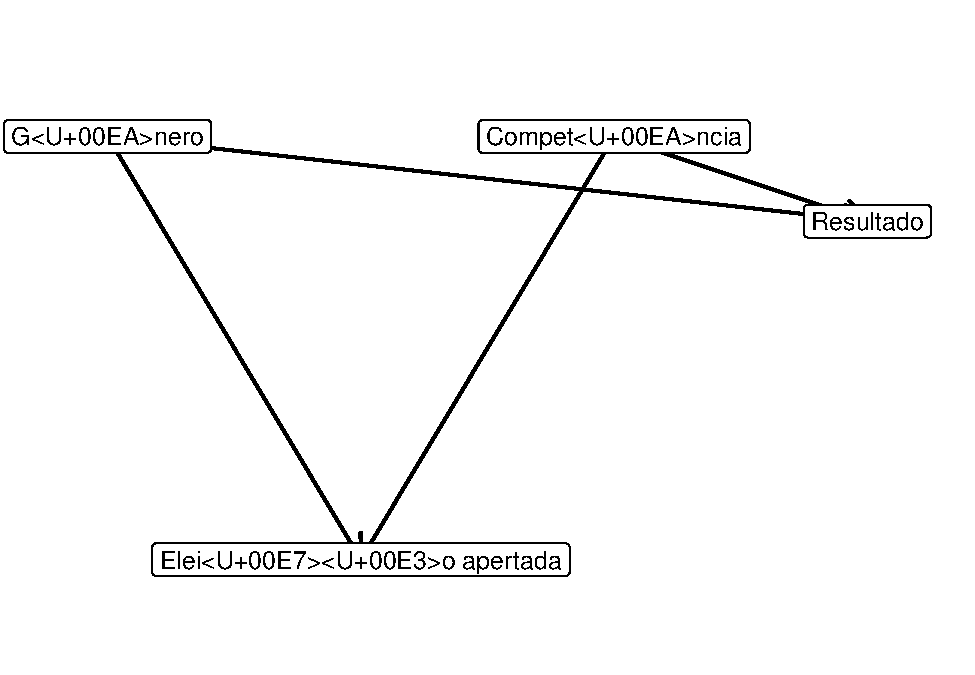
\includegraphics[alt={DAG em que g<U+00EA>nero e compet<U+00EA>ncia afetam a probabilidade de elei<U+00E7><U+00E3>o apertada e tamb<U+00E9>m o resultado, tornando elei<U+00E7><U+00E3>o apertada um collider.}]{bookdownproj_files/figure-latex/DAG-1} \caption{PCRD: condicionar em elei<U+00E7><U+00F5>es apertadas pode abrir um caminho de collider.}\label{fig:DAG}
\end{figure}

\subsection{Checklist para um paper de RDD}\label{checklist-para-um-paper-de-rdd}

\begin{enumerate}
\def\labelenumi{\arabic{enumi}.}
\item
  Descrever a regra institucional que gera o cutoff e quem poderia manipulá-la.
\item
  Definir se o desenho é sharp ou fuzzy. Em fuzzy RD, reportar a primeira etapa e interpretar o estimando como LATE local.
\item
  Apresentar gráfico RD com bins apropriados, curva local e cutoff visível.
\item
  Reportar estimativas com regressão local linear, kernel e bandwidth explícitos.
\item
  Usar inferência robusta com correção de viés, com bandwidth MSE/CER-optimal ou justificativa clara para bandwidth escolhido.
\item
  Separar a interpretação de continuidade da interpretação de aleatorização local. Bandwidth automático de \texttt{rdrobust} não define uma janela ``como se aleatória''.
\item
  Testar balanceamento de covariáveis de pré-tratamento.
\item
  Avaliar densidade da \emph{running variable} no cutoff com \texttt{rddensity}/McCrary, lembrando que falhar em rejeitar manipulação não prova ausência de manipulação.
\item
  Fazer testes placebo em cutoffs e outcomes substantivamente justificados, evitando uma pescaria de especificações.
\item
  Examinar sensibilidade a bandwidths, polinômios locais, covariáveis e \emph{donut RD} (exclusão de uma faixa muito próxima ao cutoff) quando houver risco de manipulação muito perto do cutoff.
\item
  Discutir casos difíceis: running variable discreta, clusters, múltiplos cutoffs, RD espacial, eleições apertadas ou tratamento dinâmico.
\item
  Estabelecer a validade da estratégia antes de discutir apenas resultados.
\item
  Em PCRD, não interpretar automaticamente a estimativa como efeito isolado de uma característica do político. Explicitar se a hipótese forte de Marshall é plausível; caso contrário, apresentar a estimativa como efeito composto ou como exercício de bounds/sensibilidade.
\end{enumerate}

\subsection{Referências}\label{referuxeancias-1}

Canay, I. A., \& Kamat, V. (2018). Approximate permutation tests and induced order statistics in the regression discontinuity design. The Review of Economic Studies, 85(3), 1577-1608.

Cattaneo, M. D., Idrobo, N., \& Titiunik, R. (2024). \emph{A practical introduction to regression discontinuity designs: Extensions}. Cambridge University Press. \url{https://doi.org/10.1017/9781009441896}

Cattaneo, M. D., Idrobo, N., \& Titiunik, R. (2020). \emph{A practical introduction to regression discontinuity designs: Foundations}. Cambridge University Press.

Cattaneo, M. D., Jansson, M., \& Ma, X. (2020). Simple local polynomial density estimators. \emph{Journal of the American Statistical Association}, 115(531), 1449-1455.

Cattaneo, M. D., \& Titiunik, R. (2022). Regression discontinuity designs. \emph{Annual Review of Economics}, 14, 821-851. \url{https://doi.org/10.1146/annurev-economics-051520-021409}

Cattaneo, M. D., Titiunik, R., \& Yu, R. R. (2025a). Estimation and inference in boundary discontinuity designs. arXiv:2505.05670. \url{https://arxiv.org/abs/2505.05670}

Cattaneo, M. D., Titiunik, R., \& Yu, R. R. (2025b). rd2d: Causal inference in boundary discontinuity designs. arXiv:2505.07989. \url{https://arxiv.org/abs/2505.07989}

Caughey, D., \& Sekhon, J. S. (2011). Elections and the regression discontinuity design: Lessons from close U.S. House races, 1942-2008. \emph{Political Analysis}, 19(4), 385-408.

De Magalhães, L., Hangartner, D., Hirvonen, S., Meriläinen, J., Ruiz, N. A., \& Tukiainen, J. (2025). When Can We Trust Regression Discontinuity Design Estimates from Close Elections? Evidence from Experimental Benchmarks. Political Analysis, 1-8.

De la Cuesta, B., \& Imai, K. (2016). Misunderstandings about the regression discontinuity design in the study of close elections. \emph{Annual Review of Political Science}, 19(1), 375-396.

Eckles, D., Ignatiadis, N., Wager, S., \& Wu, H. (2025). Noise-induced randomization in regression discontinuity designs. \emph{Biometrika}, 112(2), asaf003. \url{https://doi.org/10.1093/biomet/asaf003}

Erikson, R. S., \& Rader, K. (2017). Much ado about nothing: RDD and the incumbency advantage. \emph{Political Analysis}, 25(2), 269-275.

Fitzgerald, J. (2025). Manipulation tests in regression discontinuity design: The need for equivalence testing. \emph{MetaArXiv}. \url{https://doi.org/10.31219/osf.io/2dgrp_v1}

Gelman, A., \& Imbens, G. (2019). Why high-order polynomials should not be used in regression discontinuity designs. Journal of Business \& Economic Statistics, 37(3), 447-456.

Hartman, E. (2021). Equivalence testing for regression discontinuity designs. \emph{Political Analysis}, 29(4), 505-521. \url{https://doi.org/10.1017/pan.2020.43}

Hsu, Y.-C., \& Shen, S. (2024). Dynamic regression discontinuity under treatment effect heterogeneity. \emph{Quantitative Economics}, 15(4), 1035-1064. \url{https://doi.org/10.3982/QE2150}

Kreiß, A., \& Rothe, C. (2023). Inference in regression discontinuity designs with high-dimensional covariates. \emph{The Econometrics Journal}, 26(2), 105-123. \url{https://doi.org/10.1093/ectj/utac029}

Lee, D. S. (2008). Randomized experiments from non-random selection in U.S. House elections. \emph{Journal of Econometrics}, 142(2), 675-697.

Marshall, J. (2024). Can close election regression discontinuity designs identify effects of winning politician characteristics? \emph{American Journal of Political Science}, 68(2), 494-510.

McCrary, J. (2008). Manipulation of the running variable in the regression discontinuity design: A density test. \emph{Journal of Econometrics}, 142(2), 698-714.

Noack, C., Olma, T., \& Rothe, C. (2025). Flexible covariate adjustments in regression discontinuity designs. Working paper, revised April 2025. \url{https://arxiv.org/abs/2107.07942}

Noack, C., \& Rothe, C. (2024). Bias-aware inference in fuzzy regression discontinuity designs. \emph{Econometrica}, 92(3), 687-711. \url{https://doi.org/10.3982/ECTA19466}

\begin{itemize}
\tightlist
\item
  Tutorial: \url{https://congressdata.joshuamccrain.com/regression_discontinuity.html}
\end{itemize}

\section{Diferença em Diferenças}\label{diferenuxe7a-em-diferenuxe7as}

\subsection{Motivação: por que DiD?}\label{motivauxe7uxe3o-por-que-did}

Diferença em Diferenças (DiD) é o método quase-experimental mais utilizado em ciência política e economia aplicada. A ideia central é simples: se dois grupos seguem trajetórias paralelas antes de uma intervenção, a diferença nas suas trajetórias \emph{após} a intervenção pode ser atribuída ao tratamento. Para tratamentos introdutórios complementares, ver Cunningham (\citeproc{ref-cunningham2021}{2021}) e Huntington-Klein (\citeproc{ref-huntingtonklein2022}{2022}); para um exemplo clássico em economia aplicada, ver Card and Krueger (\citeproc{ref-cardkrueger1994}{1994}).

Considere um exemplo concreto. Suponha que duas cidades --- Campinas e Ribeirão Preto --- têm taxas de conclusão de obras públicas de 30\% e 20\%, respectivamente, em 2016. Em 2018, Campinas recebe um programa de monitoramento de obras, enquanto Ribeirão Preto não. Em 2018, Campinas tem taxa de 50\% e Ribeirão Preto, 35\%.

A variação temporal em Campinas é \(50\% - 30\% = 20\) p.p. Mas parte disso pode ser tendência geral --- afinal, Ribeirão Preto também cresceu \(35\% - 20\% = 15\) p.p. sem tratamento. O DiD subtrai essa tendência: \(20 - 15 = 5\) p.p. Esse é o efeito estimado do programa.

\[
\underbrace{(50 - 30)}_{\Delta \text{Campinas}} - \underbrace{(35 - 20)}_{\Delta \text{Ribeirão}} = 20 - 15 = 5 \text{ p.p.}
\]

Essa conta manual contém toda a lógica do DiD. O restante do capítulo formaliza essa intuição, discute quando ela é válida (tendências paralelas), mostra como estimar por regressão (TWFE) e apresenta os avanços metodológicos recentes para lidar com tratamento escalonado no tempo e efeitos heterogêneos.

\textbf{Mapa do capítulo.} O capítulo começa com o modelo 2×2 e seus pressupostos de identificação, incluindo tendências paralelas, escala do outcome, tendências paralelas condicionais, não-antecipação e spillovers. Em seguida, mostra como estimar DiD por TWFE, discute inferência e aplica o desenho ao Obra Transparente. A parte central trata da ``revolução DiD'': event studies, viés do TWFE com tratamento escalonado, contaminação de coeficientes dinâmicos e estimadores modernos. O capítulo termina com análise de sensibilidade, uma segunda aplicação empírica (enchente do Elbe), extensões importantes e um checklist prático de desenho.

\subsection{Modelo básico 2×2}\label{modelo-buxe1sico-22}

Considere dois grupos e dois períodos de tempo, \(t \in \{1, 2\}\). O grupo tratado recebe a intervenção no período 2; o grupo controle nunca é tratado. Seja \(D_i \in \{0, 1\}\) o indicador de pertencer ao grupo tratado.

Definimos os resultados potenciais: \(Y_{it}(0)\) é o resultado da unidade \(i\) no período \(t\) na ausência de tratamento, e \(Y_{it}(1)\) é o resultado sob tratamento. O resultado observado é \(Y_{it} = D_i \cdot \mathbb{1}[t=2] \cdot Y_{it}(1) + (1 - D_i \cdot \mathbb{1}[t=2]) \cdot Y_{it}(0)\).

O \textbf{estimando} é o efeito médio do tratamento sobre os tratados (ATT) no período pós-tratamento:

\[
\tau^{ATT} = \mathbb{E}[Y_{i2}(1) - Y_{i2}(0) \mid D_i = 1]
\]

Suponha que os resultados potenciais seguem a estrutura:

\begin{table}[!h]
\centering
\caption{\label{tab:tabela-did}Estrutura de resultados potenciais no DiD 2×2}
\centering
\begin{tabular}[t]{>{}l|cc}
\toprule
  & Pré ($t = 1$) & Pós ($t = 2$)\\
\midrule
Controle ($D_i = 0$) & $\alpha_i + \lambda_1$ & $\alpha_i + \lambda_2$\\
Tratado ($D_i = 1$) & $\alpha_i + \lambda_1$ & $\alpha_i + \lambda_2 + \tau_i$\\
\bottomrule
\end{tabular}
\end{table}

Nessa tabela, \(\alpha_i\) é o efeito fixo de unidade (nível base), \(\lambda_t\) é o efeito fixo de tempo (tendência comum), e \(\tau_i\) é o efeito causal individual. No grupo controle, \(\tau_i = 0\) por definição.

A diferença temporal para cada grupo é:

Para o grupo tratado: \(\mathbb{E}[Y_{i2} - Y_{i1} \mid D_i = 1] = (\lambda_2 - \lambda_1) + \mathbb{E}[\tau_i \mid D_i = 1]\)

Para o grupo controle: \(\mathbb{E}[Y_{i2} - Y_{i1} \mid D_i = 0] = (\lambda_2 - \lambda_1)\)

A diferença entre essas duas diferenças elimina a tendência comum:

\[
\underbrace{\mathbb{E}[Y_{i2} - Y_{i1} \mid D_i = 1]}_{\Delta \text{Tratado}} - \underbrace{\mathbb{E}[Y_{i2} - Y_{i1} \mid D_i = 0]}_{\Delta \text{Controle}} = \mathbb{E}[\tau_i \mid D_i = 1] = \tau^{ATT}
\]

O modelo básico 2×2 nos dá a intuição do DiD. Na prática, estimamos esse efeito por regressão, como veremos a seguir.

\subsection{Pressupostos de identificação}\label{pressupostos-de-identificauxe7uxe3o}

\subsubsection{Tendências paralelas}\label{tenduxeancias-paralelas}

O pressuposto central do DiD é o de \textbf{tendências paralelas} (parallel trends, PT): na ausência de tratamento, a evolução média dos resultados teria sido a mesma nos dois grupos.

\[
\mathbb{E}[Y_{i2}(0) - Y_{i1}(0) \mid D_i = 1] = \mathbb{E}[Y_{i2}(0) - Y_{i1}(0) \mid D_i = 0]
\]

\begin{figure}
\centering
\pandocbounded{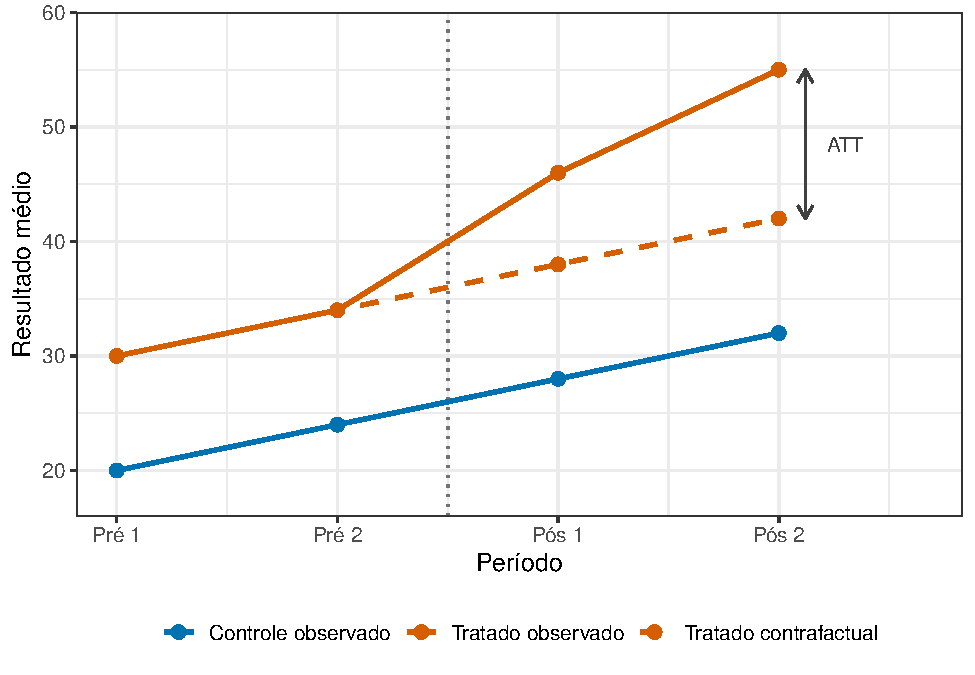
\includegraphics[keepaspectratio,alt={\label{fig:pt-classico}Tend\textless U+00EA\textgreater ncias paralelas no contrafactual sem tratamento. A linha tracejada mostra a trajet\textless U+00F3\textgreater ria que o grupo tratado teria seguido sem tratamento; ela cresce no mesmo ritmo do controle no per\textless U+00ED\textgreater odo p\textless U+00F3\textgreater s-tratamento. A dist\textless U+00E2\textgreater ncia vertical entre o tratado observado e o contrafactual no p\textless U+00F3\textgreater s \textless U+00E9\textgreater{} o ATT.}]{bookdownproj_files/figure-latex/pt-classico-1.pdf}}
\caption{\label{fig:pt-classico}Tend\textless U+00EA\textgreater ncias paralelas no contrafactual sem tratamento. A linha tracejada mostra a trajet\textless U+00F3\textgreater ria que o grupo tratado teria seguido sem tratamento; ela cresce no mesmo ritmo do controle no per\textless U+00ED\textgreater odo p\textless U+00F3\textgreater s-tratamento. A dist\textless U+00E2\textgreater ncia vertical entre o tratado observado e o contrafactual no p\textless U+00F3\textgreater s \textless U+00E9\textgreater{} o ATT.}
\end{figure}

Na Figura \ref{fig:pt-classico}, os grupos começam em níveis diferentes. Isso não viola DiD. A suposição é que, sem tratamento, o grupo tratado teria continuado em uma trajetória paralela à do grupo controle. O efeito causal é a distância entre a trajetória observada dos tratados e essa trajetória contrafactual no período pós-tratamento.

Note que o lado esquerdo envolve um contrafactual --- o que \emph{teria acontecido} com os tratados sem tratamento --- e portanto não é diretamente testável. Podemos verificar se as tendências foram paralelas no período \emph{pré}-tratamento (o que é necessário mas não suficiente), mas não podemos verificar se continuariam paralelas no período pós.

\subsubsection{Tendências paralelas em qual escala?}\label{tenduxeancias-paralelas-em-qual-escala}

O pressuposto de tendências paralelas é uma restrição sobre a forma funcional do resultado. Dizer que tratados e controles teriam tendências paralelas em \textbf{níveis} não é o mesmo que dizer que teriam tendências paralelas em \textbf{logs}, percentuais, taxas padronizadas ou qualquer outra transformação. Se duas unidades crescem pela mesma quantidade absoluta, suas trajetórias são paralelas em níveis; se crescem pela mesma taxa percentual, são paralelas em logs. As duas coisas só coincidem em casos especiais.

Isso importa porque o DiD não é automaticamente invariante à transformação do outcome. Uma política pode parecer aumentar \(Y\) em 5 pontos percentuais em níveis, mas parecer ter efeito proporcional diferente se estimarmos \(\log(Y)\); e a transformação também muda qual trajetória contrafactual estamos supondo. Roth and Sant'Anna (\citeproc{ref-rothsantanna2023}{2023}) mostram que, para identificar pontualmente o ATT, o pesquisador precisa justificar por que a forma funcional escolhida é a correta, por que o tratamento é plausivelmente quase aleatório, ou usar uma estratégia que recupere a distribuição contrafactual inteira. Hull (\citeproc{ref-hull2024metrix}{2024}) enfatiza essa pergunta de forma pedagógica como: ``tendências paralelas em quê?''.

\textbf{Regra prática:} escolha a escala do outcome antes de olhar os resultados, explique a teoria substantiva por trás da escolha e, quando a escala for discutível, reporte a sensibilidade dos resultados a transformações plausíveis. Não trate logs como uma escolha puramente técnica.

\subsubsection{Equivalência entre PT e TWFE}\label{equivaluxeancia-entre-pt-e-twfe}

Uma forma paramétrica equivalente é supor que os resultados potenciais sem tratamento seguem um modelo de efeitos fixos duplos:

\[
Y_{it}(0) = \alpha_i + \lambda_t + \varepsilon_{it}, \quad \text{com } \mathbb{E}[\varepsilon_{it}] = 0
\]

\textbf{Proposição.} O modelo TWFE implica tendências paralelas, e vice-versa.

\emph{Prova (TWFE \(\Rightarrow\) PT).} Se \(Y_{it}(0) = \alpha_i + \lambda_t + \varepsilon_{it}\), então:

\[
\mathbb{E}[Y_{i2}(0) - Y_{i1}(0) \mid D_i = d] = (\alpha_i + \lambda_2) - (\alpha_i + \lambda_1) = \lambda_2 - \lambda_1
\]

para \(d \in \{0, 1\}\). Como a diferença \(\lambda_2 - \lambda_1\) não depende de \(d\), PT é satisfeita. \(\square\)

\emph{Prova (PT \(\Rightarrow\) TWFE).} Defina \(\lambda_1 \equiv 0\) (normalização) e \(\alpha_i \equiv \mathbb{E}[Y_{i1}(0)]\). Para qualquer \(t\), defina:

\[
\lambda_t \equiv \mathbb{E}[Y_{i^*t}(0) - Y_{i^*1}(0)]
\]

onde \(i^*\) é uma unidade de referência arbitrária (por exemplo, do grupo controle). Pela suposição de PT, \(\mathbb{E}[Y_{it}(0) - Y_{i1}(0)]\) é igual para todas as unidades, então:

\[
\mathbb{E}[Y_{it}(0)] = \mathbb{E}[Y_{i1}(0)] + \lambda_t = \alpha_i + \lambda_t
\]

Definindo \(\varepsilon_{it} = Y_{it}(0) - \alpha_i - \lambda_t\), temos \(\mathbb{E}[\varepsilon_{it}] = 0\) por construção. \(\square\)

\subsubsection{Tendências paralelas condicionais e covariáveis}\label{tenduxeancias-paralelas-condicionais-e-covariuxe1veis}

Em muitas aplicações, o pressuposto de tendências paralelas incondicional é forte demais: os grupos tratado e controle diferem em características observáveis que afetam a trajetória do resultado. Incluir covariáveis pode tornar o pressuposto mais plausível, mas \emph{como} incluí-las importa muito. Há duas abordagens conceitualmente distintas, e uma armadilha comum que deve ser evitada.

\paragraph{\texorpdfstring{Abordagem 1: Enriquecer o modelo de \(Y(0)\)}{Abordagem 1: Enriquecer o modelo de Y(0)}}\label{abordagem-1-enriquecer-o-modelo-de-y0}

Borusyak, Jaravel, and Spiess (\citeproc{ref-borusyak2024}{2024}) propõem enriquecer o modelo de resultados potenciais não-tratados:
\[
\mathbb{E}[Y_{it}(0)] = \alpha_i + \beta_t + \gamma' X_{it}
\]

Esse modelo é mais flexível que o TWFE aditivo puro e permite incluir:

\begin{itemize}
\tightlist
\item
  \textbf{Covariáveis contínuas}: variáveis que afetam o nível de \(Y\) (evitando maus controles, como veremos abaixo)
\item
  \textbf{Tendências lineares específicas por unidade}: \(\gamma_i \cdot t\), de modo que cada unidade tenha sua própria tendência temporal
\item
  \textbf{Interações tempo \(\times\) baseline}: \(\gamma'_t X_i\), por exemplo, efeitos fixos de estado \(\times\) ano em um painel de condados
\end{itemize}

A chave é que os parâmetros \(\gamma\) são estimados \textbf{usando apenas as observações não-tratadas} (\(D_{it} = 0\)). Depois, o contrafactual \(\hat{Y}_{it}(0)\) é imputado para as observações tratadas. Isso evita o problema de contaminar a estimativa de \(\gamma\) com efeitos do tratamento.

\paragraph{Abordagem 2: Tendências paralelas condicionais}\label{abordagem-2-tenduxeancias-paralelas-condicionais}

Uma segunda abordagem, desenvolvida por Abadie (\citeproc{ref-abadie2005}{2005}) e Sant'Anna and Zhao (\citeproc{ref-santannazhao2020}{2020}) para o caso não-escalonado, condiciona as tendências paralelas em características baseline \(X_i\):

\[
\mathbb{E}[Y_{it}(0) - Y_{it-1}(0) \mid D_i = 1, X_i] = \mathbb{E}[Y_{it}(0) - Y_{it-1}(0) \mid D_i = 0, X_i]
\]

Ou seja, as tendências são paralelas \emph{dentro de estratos} definidos por \(X_i\). Isso transforma o problema em uma versão de seleção em observáveis para \(\Delta Y_{it}\). Há três abordagens principais para estimar o DiD condicional:

\begin{enumerate}
\def\labelenumi{\arabic{enumi}.}
\tightlist
\item
  \textbf{Ponderação por propensity score inverso (IPW):} ponderar as unidades de controle para que a distribuição de \(X\) replique a do grupo tratado (\citeproc{ref-abadie2005}{Abadie 2005}).
\item
  \textbf{Regressão de resultado (\emph{outcome regression}):} modelar \(\mathbb{E}[\Delta Y_{it}(0) \mid X_i]\) parametricamente.
\item
  \textbf{Duplamente robusta (\emph{doubly robust}):} combinar IPW e regressão. Consistente se \emph{qualquer uma} das duas especificações estiver correta. O pacote \texttt{did} implementa essa abordagem (\citeproc{ref-santannazhao2020}{Sant'Anna and Zhao 2020}).
\end{enumerate}

Callaway and Sant'Anna (\citeproc{ref-callawaysantanna2021}{2021}) estendem essa lógica para tratamento escalonado, estimando um propensity score separado para cada coorte e período. Wooldridge (\citeproc{ref-wooldridge2021}{2021}) propõe uma extensão do TWFE (\emph{extended TWFE}) que inclui interações entre os efeitos fixos de tempo e as covariáveis, obtendo resultados robustos a efeitos heterogêneos sob certas condições.

\paragraph{O que não fazer: covariáveis no TWFE ingenuamente}\label{o-que-nuxe3o-fazer-covariuxe1veis-no-twfe-ingenuamente}

A prática mais comum na pesquisa aplicada é simplesmente adicionar covariáveis à regressão TWFE:
\[
Y_{it} = \alpha_i + \beta_t + \tau D_{it} + \gamma' X_{it} + \varepsilon_{it}
\]

Essa abordagem é problemática por múltiplas razões, mesmo no caso mais simples de dois períodos:

\begin{enumerate}
\def\labelenumi{\arabic{enumi}.}
\item
  \textbf{Contaminação por efeitos do tratamento.} Com efeitos heterogêneos, \(\hat{\gamma}\) é estimado usando \emph{todas} as observações, inclusive as tratadas. Isso pode atribuir indevidamente parte do efeito do tratamento às covariáveis, enviesando tanto \(\hat{\gamma}\) quanto \(\hat{\tau}\) (\citeproc{ref-borusyak2024}{Borusyak, Jaravel, and Spiess 2024}; \citeproc{ref-caetano2024}{Caetano et al. 2024}).
\item
  \textbf{Covariáveis variantes no tempo como bad controls.} Quando \(X_{it}\) pode ser afetado pelo próprio tratamento, por exemplo emprego quando o tratamento é um programa social, incluí-lo como controle introduz viés de variável intermediária: o clássico problema de \emph{bad controls} (\citeproc{ref-angrist2009}{Angrist and Pischke 2009}). A sabedoria convencional de simplesmente ``não incluir'' essas variáveis também é insuficiente: quando o PTA condicional depende dessas covariáveis, omiti-las viola a suposição de identificação (\citeproc{ref-caetano2024}{Caetano et al. 2024}).
\item
  \textbf{Covariate effect bias.} Lin and Zhang (\citeproc{ref-linzhang2022}{2022}) mostram que, mesmo com efeitos do tratamento homogêneos e apenas dois períodos, a inclusão de covariáveis variantes no tempo no TWFE gera um viés adicional, o \emph{covariate effect bias}. O problema não depende de efeitos dinâmicos do tratamento; ele surge quando o efeito das covariáveis sobre \(Y(0)\) pode variar no tempo, enquanto a regressão impõe um coeficiente comum para essas covariáveis. Esse viés persiste mesmo quando o tratamento não afeta as covariáveis.
\item
  \textbf{Reversão de pesos.} Covariáveis com valores incomuns no grupo tratado, relativo ao controle, podem receber pesos desproporcionais na regressão, distorcendo a estimativa do ATT.
\end{enumerate}

\paragraph{Baseline vs.~time-varying: uma distinção crucial}\label{baseline-vs.-time-varying-uma-distinuxe7uxe3o-crucial}

A distinção entre covariáveis \textbf{baseline} (\(X_i\), fixas ou medidas antes do tratamento) e \textbf{variantes no tempo} (\(X_{it}\), que mudam ao longo do tempo) é fundamental:

\begin{itemize}
\item
  \textbf{Covariáveis baseline} (\(X_i\)) são seguras de incluir: não podem ser afetadas pelo tratamento e não geram o problema de bad controls. São absorvidas pelos efeitos fixos de unidade em um painel, mas podem entrar via interações com o tempo (\(\gamma'_t X_i\)) ou no propensity score da abordagem 2.
\item
  \textbf{Covariáveis variantes no tempo} (\(X_{it}\)) exigem cautela. Se o tratamento pode afetar \(X_{it}\), incluí-la diretamente é um bad control. Caetano et al. (\citeproc{ref-caetano2024}{2024}) propõem estratégias que lidam com covariáveis variantes no tempo que podem ser afetadas pelo tratamento, incluindo estimandos duplamente robustos e abordagens de imputação que usam o valor que a covariável \emph{teria tido na ausência de tratamento}.
\end{itemize}

\textbf{Regra prática:} sempre que possível, use a abordagem 1, enriquecendo o modelo de \(Y(0)\) com estimação apenas nos não-tratados, ou a abordagem 2, PT condicional com covariáveis baseline e estimação duplamente robusta. Evite adicionar covariáveis variantes no tempo diretamente ao TWFE.

\subsubsection{Não-antecipação}\label{nuxe3o-antecipauxe7uxe3o}

O segundo pressuposto é de \textbf{não-antecipação}: o tratamento não tem efeito antes de ser implementado.

\[
\mathbb{E}[Y_{i1}(0)] = \mathbb{E}[Y_{i1}(1)] \quad \forall i
\]

Isso exclui, por exemplo, que a mera expectativa de um programa futuro altere o comportamento das unidades tratadas antes do programa começar. Em muitas aplicações em ciência política, esse pressuposto é plausível quando a intervenção é inesperada ou quando não há incentivo para reagir antecipadamente.

\subsubsection{Spillovers e nível de atribuição}\label{spillovers-e-nuxedvel-de-atribuiuxe7uxe3o}

O DiD também exige que o tratamento de uma unidade não altere o resultado de outra unidade usada como controle. Essa é a versão de SUTVA relevante para desenhos de painel. Se uma política implementada em municípios tratados muda o comportamento de municípios de controle, o grupo controle deixa de representar a trajetória contrafactual sem tratamento.

O nível de atribuição do tratamento também define a inferência. No caso Obra Transparente, o tratamento ocorre no nível municipal, embora os dados estejam no nível da obra. As obras dentro do mesmo município não são unidades independentes de atribuição. Por isso, a incerteza deve ser calculada no nível do município, e a interpretação causal deve tratar o município como a unidade exposta ao tratamento.

Choques comuns não invalidam o DiD. O problema surge quando choques no período pós-tratamento afetam diferentemente tratados e controles, alterando a tendência contrafactual relativa entre os grupos.

\subsection{Estimação por TWFE}\label{estimauxe7uxe3o-por-twfe}

No caso 2×2, o DiD pode ser estimado por regressão de duas formas equivalentes.

\textbf{Parametrização por interação:}

\[
Y_{it} = \beta_0 + \beta_1 \text{Post}_t + \beta_2 \text{Treat}_i + \tau (\text{Post}_t \times \text{Treat}_i) + \varepsilon_{it}
\]

onde \(\text{Post}_t = \mathbb{1}[t = 2]\) e \(\text{Treat}_i = D_i\).

\textbf{Parametrização por efeitos fixos (TWFE):}

\[
Y_{it} = \alpha_i + \lambda_t + \tau D_{it} + \varepsilon_{it}
\]

onde \(D_{it} = D_i \cdot \mathbb{1}[t = 2]\) é o indicador de tratamento efetivo.

No caso 2×2, as duas parametrizações produzem estimativas idênticas de \(\hat{\tau}\). A segunda é chamada \emph{two-way fixed effects} (TWFE) porque inclui efeitos fixos de unidade (\(\alpha_i\)) e de tempo (\(\lambda_t\)).

\textbf{Importante:} no caso 2×2, o TWFE é inofensivo --- ele recupera exatamente o ATT. Os problemas surgem quando o tratamento é adotado em momentos diferentes por diferentes unidades (\emph{staggered treatment}), como veremos na seção 7.

\subsection{Inferência em DiD}\label{inferuxeancia-em-did}

A estimativa pontual de DiD é apenas metade do problema. Em painéis, os erros normalmente são correlacionados ao longo do tempo dentro da mesma unidade, e o tratamento muitas vezes é atribuído em nível agregado: municípios, estados, escolas, firmas, distritos eleitorais etc. Ignorar essa estrutura faz os erros-padrão parecerem menores do que são.

Bertrand, Duflo, and Mullainathan (\citeproc{ref-bertrand2004}{2004}) mostram o problema com placebos em painéis estaduais: quando há autocorrelação serial e tratamento persistente, erros-padrão robustos convencionais rejeitam a hipótese nula com frequência muito maior do que 5\%. A recomendação prática é clusterizar no nível da variação de tratamento ou da atribuição da política. Se a política varia por estado, clusterize por estado; se varia por município, clusterize por município; se os dados estão no nível individual, mas o tratamento é municipal, a unidade relevante para inferência continua sendo o município.

Essa regra tem duas implicações importantes. Primeiro, o número efetivo de observações para inferência é o número de clusters, não o número de linhas do banco. Um painel com milhões de indivíduos, mas 20 municípios tratados/controles, tem pouca informação independente para inferência. Segundo, ``clusterizar no nível mais baixo'' quase nunca é conservador quando a política é atribuída em nível mais alto: clusterizar por obra, aluno ou indivíduo ignora que todos dentro do mesmo município ou estado receberam a mesma política.

Quando há poucos clusters --- especialmente poucos clusters tratados --- os erros-padrão clusterizados assintóticos podem continuar ruins. Nesse caso, considere wild cluster bootstrap, inferência por randomização quando o mecanismo de atribuição é defensável, ou uma apresentação mais honesta de incerteza baseada no número de clusters. Em event studies, também faz sentido distinguir intervalos ponto-a-ponto de bandas simultâneas: se vários coeficientes de pré-tratamento são inspecionados ao mesmo tempo, bandas simultâneas comunicam melhor a incerteza conjunta (\citeproc{ref-freyaldenhoven2019}{Freyaldenhoven, Hansen, and Shapiro 2019}; \citeproc{ref-goldsmithpinkham2026applied}{Goldsmith-Pinkham 2026}).

\textbf{Nota sobre wild cluster bootstrap.} O wild cluster bootstrap não sorteia observações individuais nem clusters inteiros. Ele mantém os clusters fixos e multiplica os resíduos de cada cluster por pesos aleatórios, frequentemente \(+1\) ou \(-1\). Todos os resíduos dentro do mesmo cluster recebem o mesmo peso, preservando a correlação interna. Com esses resíduos reponderados, criamos muitos outcomes simulados, reestimamos o modelo e usamos a distribuição bootstrap da estatística de teste para calcular p-valores ou intervalos. A vantagem sobre o bootstrap clusterizado comum é que, com poucos clusters, sortear clusters com reposição pode gerar amostras artificiais ruins, repetindo muito alguns clusters e excluindo outros. O wild cluster bootstrap costuma produzir inferência mais confiável quando há poucos clusters ou poucos clusters tratados, embora ainda dependa de o nível de clusterização corresponder ao nível de atribuição do tratamento.

\subsection{Aplicação 1: Obra Transparente}\label{aplicauxe7uxe3o-1-obra-transparente}

Vamos aplicar o DiD a dados reais brasileiros usando a versão submetida ao \emph{Journal of Development Studies} do paper sobre o projeto Obra Transparente. A intervenção foi conduzida pela Transparência Brasil entre maio de 2017 e junho de 2019, em parceria com 21 organizações locais da sociedade civil em municípios do Sul e Sudeste. Essas organizações receberam treinamento e apoio para monitorar obras de creches e escolas financiadas pelo FNDE.

O outcome é binário: a obra estava concluída naquele período ou não. A unidade observada é a obra, mas o tratamento é municipal. O painel é balanceado, com seis períodos entre agosto de 2015 e outubro de 2023. O monitoramento ativo começa em setembro de 2018, que codificamos como o primeiro período tratado.

\begin{Shaded}
\begin{Highlighting}[]
\FunctionTok{library}\NormalTok{(here, }\AttributeTok{quietly =} \ConstantTok{TRUE}\NormalTok{)}
\FunctionTok{library}\NormalTok{(knitr)}
\FunctionTok{library}\NormalTok{(kableExtra)}
\FunctionTok{library}\NormalTok{(tidyverse)}
\FunctionTok{library}\NormalTok{(fixest)}

\NormalTok{ot\_root }\OtherTok{\textless{}{-}} \FunctionTok{here}\NormalTok{(}\StringTok{"data"}\NormalTok{, }\StringTok{"obra\_transparente\_jds"}\NormalTok{, }\StringTok{"replication\_package"}\NormalTok{)}
\NormalTok{ot\_panel\_file }\OtherTok{\textless{}{-}} \FunctionTok{file.path}\NormalTok{(ot\_root, }\StringTok{"data"}\NormalTok{, }\StringTok{"processed"}\NormalTok{, }\StringTok{"did\_panel\_6periods.rds"}\NormalTok{)}
\NormalTok{ot\_results\_file }\OtherTok{\textless{}{-}} \FunctionTok{file.path}\NormalTok{(ot\_root, }\StringTok{"data"}\NormalTok{, }\StringTok{"processed"}\NormalTok{, }\StringTok{"did\_results\_6periods.rds"}\NormalTok{)}

\ControlFlowTok{if}\NormalTok{ (}\SpecialCharTok{!}\FunctionTok{file.exists}\NormalTok{(ot\_panel\_file) }\SpecialCharTok{||} \SpecialCharTok{!}\FunctionTok{file.exists}\NormalTok{(ot\_results\_file)) \{}
  \FunctionTok{source}\NormalTok{(}\FunctionTok{here}\NormalTok{(}\StringTok{"scripts"}\NormalTok{, }\StringTok{"prepare\_obra\_transparente\_jds.R"}\NormalTok{))}
\NormalTok{\}}

\NormalTok{did\_panel }\OtherTok{\textless{}{-}} \FunctionTok{readRDS}\NormalTok{(ot\_panel\_file)}
\NormalTok{did\_results }\OtherTok{\textless{}{-}} \FunctionTok{readRDS}\NormalTok{(ot\_results\_file)}

\NormalTok{completion\_rates }\OtherTok{\textless{}{-}}\NormalTok{ readr}\SpecialCharTok{::}\FunctionTok{read\_csv}\NormalTok{(}
  \FunctionTok{file.path}\NormalTok{(ot\_root, }\StringTok{"output"}\NormalTok{, }\StringTok{"tables"}\NormalTok{, }\StringTok{"table2\_completion\_rates.csv"}\NormalTok{),}
  \AttributeTok{show\_col\_types =} \ConstantTok{FALSE}
\NormalTok{)}

\NormalTok{wild\_results }\OtherTok{\textless{}{-}}\NormalTok{ readr}\SpecialCharTok{::}\FunctionTok{read\_csv}\NormalTok{(}
  \FunctionTok{file.path}\NormalTok{(ot\_root, }\StringTok{"output"}\NormalTok{, }\StringTok{"tables"}\NormalTok{, }\StringTok{"wild\_bootstrap\_results.csv"}\NormalTok{),}
  \AttributeTok{show\_col\_types =} \ConstantTok{FALSE}
\NormalTok{)}

\NormalTok{period\_labels }\OtherTok{\textless{}{-}} \FunctionTok{c}\NormalTok{(}
  \StringTok{"0"} \OtherTok{=} \StringTok{"Ago/2015"}\NormalTok{,}
  \StringTok{"1"} \OtherTok{=} \StringTok{"Mai/2017"}\NormalTok{,}
  \StringTok{"2"} \OtherTok{=} \StringTok{"Mar/2018"}\NormalTok{,}
  \StringTok{"3"} \OtherTok{=} \StringTok{"Set/2018"}\NormalTok{,}
  \StringTok{"4"} \OtherTok{=} \StringTok{"Ago/2019"}\NormalTok{,}
  \StringTok{"5"} \OtherTok{=} \StringTok{"Out/2023"}
\NormalTok{)}

\NormalTok{panel\_summary }\OtherTok{\textless{}{-}}\NormalTok{ tibble}\SpecialCharTok{::}\FunctionTok{tibble}\NormalTok{(}
  \AttributeTok{Medida =} \FunctionTok{c}\NormalTok{(}\StringTok{"Obras"}\NormalTok{, }\StringTok{"Municípios"}\NormalTok{, }\StringTok{"Municípios tratados"}\NormalTok{, }\StringTok{"Períodos"}\NormalTok{),}
  \AttributeTok{Valor =} \FunctionTok{c}\NormalTok{(}
\NormalTok{    dplyr}\SpecialCharTok{::}\FunctionTok{n\_distinct}\NormalTok{(did\_panel}\SpecialCharTok{$}\NormalTok{id),}
\NormalTok{    dplyr}\SpecialCharTok{::}\FunctionTok{n\_distinct}\NormalTok{(did\_panel}\SpecialCharTok{$}\NormalTok{municipio),}
\NormalTok{    dplyr}\SpecialCharTok{::}\FunctionTok{n\_distinct}\NormalTok{(did\_panel}\SpecialCharTok{$}\NormalTok{municipio[did\_panel}\SpecialCharTok{$}\NormalTok{group\_treated }\SpecialCharTok{==} \DecValTok{1}\NormalTok{]),}
\NormalTok{    dplyr}\SpecialCharTok{::}\FunctionTok{n\_distinct}\NormalTok{(did\_panel}\SpecialCharTok{$}\NormalTok{periodo)}
\NormalTok{  )}
\NormalTok{)}

\NormalTok{panel\_summary }\SpecialCharTok{\%\textgreater{}\%}
  \FunctionTok{kable}\NormalTok{(}\AttributeTok{caption =} \StringTok{"Estrutura do painel Obra Transparente — versão JDS"}\NormalTok{)}
\end{Highlighting}
\end{Shaded}

\begin{table}

\caption{\label{tab:ot-import}Estrutura do painel Obra Transparente — versão JDS}
\centering
\begin{tabular}[t]{l|r}
\hline
Medida & Valor\\
\hline
Obras & 3494\\
\hline
Municípios & 1845\\
\hline
Municípios tratados & 21\\
\hline
Períodos & 6\\
\hline
\end{tabular}
\end{table}

Antes da regressão, olhe a conta descritiva. Os municípios tratados começam com taxa de conclusão bem menor que a dos controles. Isso não invalida o DiD: o pressuposto é sobre tendências contrafactuais, não sobre igualdade de níveis.

\begin{Shaded}
\begin{Highlighting}[]
\NormalTok{completion\_rates }\SpecialCharTok{\%\textgreater{}\%}
  \FunctionTok{mutate}\NormalTok{(}\AttributeTok{periodo\_label =}\NormalTok{ period\_labels[}\FunctionTok{as.character}\NormalTok{(periodo)]) }\SpecialCharTok{\%\textgreater{}\%}
\NormalTok{  dplyr}\SpecialCharTok{::}\FunctionTok{select}\NormalTok{(}
\NormalTok{    periodo\_label,}
    \AttributeTok{controle =}\NormalTok{ Control,}
    \AttributeTok{tratamento =}\NormalTok{ Treatment,}
    \AttributeTok{diferenca =}\NormalTok{ Diff,}
    \AttributeTok{did =}\NormalTok{ DiD}
\NormalTok{  ) }\SpecialCharTok{\%\textgreater{}\%}
  \FunctionTok{kable}\NormalTok{(}
    \AttributeTok{caption =} \StringTok{"Taxa de conclusão de obras por período e grupo (\%)"}\NormalTok{,}
    \AttributeTok{digits =} \DecValTok{1}\NormalTok{,}
    \AttributeTok{col.names =} \FunctionTok{c}\NormalTok{(}\StringTok{"Período"}\NormalTok{, }\StringTok{"Controle"}\NormalTok{, }\StringTok{"Tratamento"}\NormalTok{, }\StringTok{"Diferença"}\NormalTok{, }\StringTok{"DiD"}\NormalTok{)}
\NormalTok{  )}
\end{Highlighting}
\end{Shaded}

\textbackslash begin\{table\}

\textbackslash caption\{\label{tab:ot-completion-rates}Taxa de conclusão de obras por período e grupo (\%)\}
\centering

\begin{tabular}[t]{l|r|r|r|r}
\hline
Período & Controle & Tratamento & Diferença & DiD\\
\hline
Ago/2015 & 44.6 & 17.6 & -27.1 & NA\\
\hline
Mai/2017 & 55.4 & 29.8 & -25.6 & 1.5\\
\hline
Mar/2018 & 57.2 & 31.4 & -25.8 & -0.2\\
\hline
Set/2018 & 59.1 & 35.1 & -24.0 & 1.8\\
\hline
Ago/2019 & 62.0 & 40.4 & -21.6 & 2.4\\
\hline
Out/2023 & 86.5 & 78.7 & -7.8 & 13.9\\
\hline
\end{tabular}

\textbackslash end\{table\}

O gráfico abaixo mostra a evolução da taxa de conclusão por grupo. As diferenças de nível são grandes, mas as tendências pré-tratamento são próximas. O salto maior aparece no último período, em outubro de 2023, o que também exige cautela substantiva: esse intervalo inclui a pandemia de COVID-19.

\begin{figure}
\centering
\pandocbounded{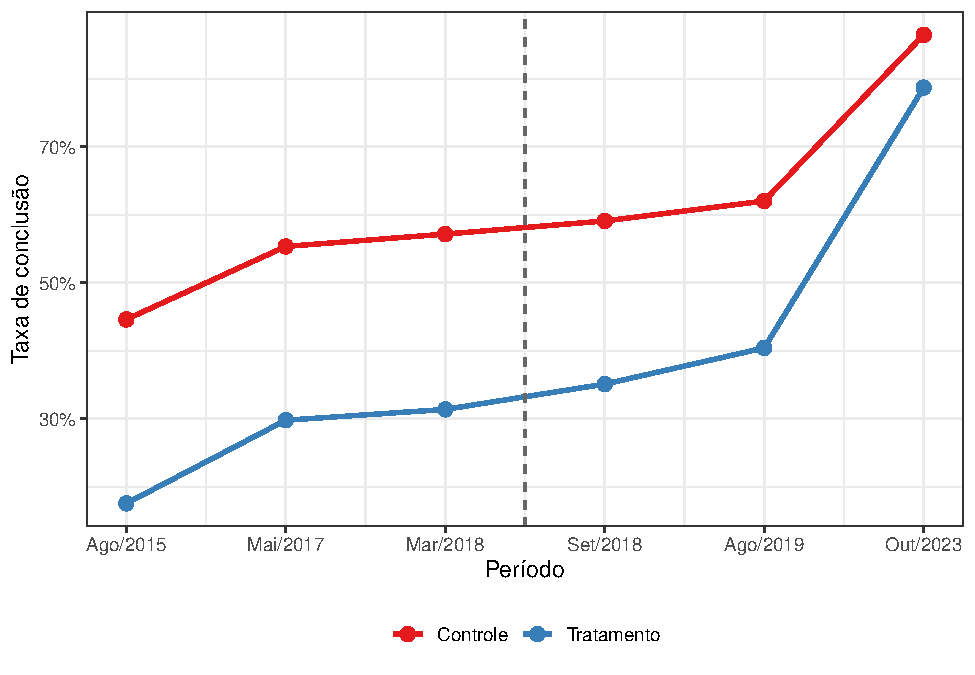
\includegraphics[keepaspectratio,alt={\label{fig:ot-tendencias}Evolu\textless U+00E7\textgreater\textless U+00E3\textgreater o da taxa de conclus\textless U+00E3\textgreater o de obras por grupo. Linha vertical indica o in\textless U+00ED\textgreater cio do tratamento em setembro de 2018.}]{bookdownproj_files/figure-latex/ot-tendencias-1.pdf}}
\caption{\label{fig:ot-tendencias}Evolu\textless U+00E7\textgreater\textless U+00E3\textgreater o da taxa de conclus\textless U+00E3\textgreater o de obras por grupo. Linha vertical indica o in\textless U+00ED\textgreater cio do tratamento em setembro de 2018.}
\end{figure}

O modelo estático do paper usa todos os seis períodos e compara a média dos períodos pós-tratamento com a trajetória contrafactual estimada a partir dos controles. A especificação inclui efeitos fixos de obra e de período:

\[
Y_{it} = \alpha_i + \lambda_t + \tau(\text{Tratado}_i \times \text{Pós}_t) + \varepsilon_{it}.
\]

\begin{Shaded}
\begin{Highlighting}[]
\NormalTok{did\_ot\_static }\OtherTok{\textless{}{-}} \FunctionTok{feols}\NormalTok{(}
\NormalTok{  concluida }\SpecialCharTok{\textasciitilde{}}\NormalTok{ treat\_post }\SpecialCharTok{|}\NormalTok{ id }\SpecialCharTok{+}\NormalTok{ periodo,}
  \AttributeTok{data =}\NormalTok{ did\_panel,}
  \AttributeTok{cluster =} \SpecialCharTok{\textasciitilde{}}\NormalTok{municipio}
\NormalTok{)}

\NormalTok{ot\_static\_coef }\OtherTok{\textless{}{-}} \FunctionTok{coeftable}\NormalTok{(did\_ot\_static)}
\NormalTok{ot\_static\_est }\OtherTok{\textless{}{-}} \FunctionTok{unname}\NormalTok{(ot\_static\_coef[}\StringTok{"treat\_post"}\NormalTok{, }\StringTok{"Estimate"}\NormalTok{])}
\NormalTok{ot\_static\_se }\OtherTok{\textless{}{-}} \FunctionTok{unname}\NormalTok{(ot\_static\_coef[}\StringTok{"treat\_post"}\NormalTok{, }\StringTok{"Std. Error"}\NormalTok{])}
\NormalTok{ot\_static\_p }\OtherTok{\textless{}{-}} \FunctionTok{unname}\NormalTok{(ot\_static\_coef[}\StringTok{"treat\_post"}\NormalTok{, }\StringTok{"Pr(\textgreater{}|t|)"}\NormalTok{])}

\NormalTok{tibble}\SpecialCharTok{::}\FunctionTok{tibble}\NormalTok{(}
  \AttributeTok{Estimando =} \StringTok{"ATT médio pós{-}tratamento"}\NormalTok{,}
  \AttributeTok{Estimativa =} \FunctionTok{round}\NormalTok{(ot\_static\_est, }\DecValTok{3}\NormalTok{),}
  \StringTok{\textasciigrave{}}\AttributeTok{Erro{-}padrão}\StringTok{\textasciigrave{}} \OtherTok{=} \FunctionTok{round}\NormalTok{(ot\_static\_se, }\DecValTok{3}\NormalTok{),}
  \StringTok{\textasciigrave{}}\AttributeTok{IC 95\%}\StringTok{\textasciigrave{}} \OtherTok{=} \FunctionTok{sprintf}\NormalTok{(}
    \StringTok{"[\%.3f, \%.3f]"}\NormalTok{,}
\NormalTok{    ot\_static\_est }\SpecialCharTok{{-}} \FloatTok{1.96} \SpecialCharTok{*}\NormalTok{ ot\_static\_se,}
\NormalTok{    ot\_static\_est }\SpecialCharTok{+} \FloatTok{1.96} \SpecialCharTok{*}\NormalTok{ ot\_static\_se}
\NormalTok{  ),}
  \StringTok{\textasciigrave{}}\AttributeTok{p{-}valor}\StringTok{\textasciigrave{}} \OtherTok{=} \FunctionTok{round}\NormalTok{(ot\_static\_p, }\DecValTok{3}\NormalTok{),}
\NormalTok{  Interpretação }\OtherTok{=} \StringTok{"Aumento médio de 8,3 p.p. na conclusão das obras"}
\NormalTok{) }\SpecialCharTok{\%\textgreater{}\%}
  \FunctionTok{kable}\NormalTok{(}
    \AttributeTok{caption =} \StringTok{"DiD estático — Obra Transparente (versão JDS)"}
\NormalTok{  )}
\end{Highlighting}
\end{Shaded}

\begin{table}

\caption{\label{tab:ot-did-estatico}DiD estático — Obra Transparente (versão JDS)}
\centering
\begin{tabular}[t]{l|r|r|l|r|l}
\hline
Estimando & Estimativa & Erro-padrão & IC 95\% & p-valor & Interpretação\\
\hline
ATT médio pós-tratamento & 0.083 & 0.034 & [0.017, 0.150] & 0.013 & Aumento médio de 8,3 p.p. na conclusão das obras\\
\hline
\end{tabular}
\end{table}

O coeficiente estima um aumento médio de cerca de 8,3 pontos percentuais na probabilidade de conclusão das obras nos municípios tratados. Essa é a estimativa estática: ela resume todos os períodos pós-tratamento em um único número. A próxima pergunta é dinâmica: o efeito aparece imediatamente ou cresce ao longo do tempo?

\subsection{DiD dinâmico e event study}\label{did-dinuxe2mico-e-event-study}

Na prática, raramente temos apenas dois períodos. Com múltiplos períodos, podemos estimar um \textbf{event study} (estudo de evento) que mostra a dinâmica do efeito ao longo do tempo. A especificação é:

\[
Y_{it} = \alpha_i + \lambda_t + \sum_{k \neq -1} \delta_k \cdot \mathbb{1}[t - G_i = k] + \varepsilon_{it}
\]

onde \(G_i\) é o período em que a unidade \(i\) é primeiro tratada (com \(G_i = \infty\) para nunca-tratados), e \(k\) mede a distância ao tratamento (tempo relativo). O período \(k = -1\) (um antes do tratamento) é a categoria de referência.

Os coeficientes \(\delta_k\) têm interpretação direta:

\begin{itemize}
\tightlist
\item
  Para \(k < -1\) (pré-tratamento): se as tendências são paralelas, devemos ter \(\delta_k \approx 0\). Esses coeficientes servem como \textbf{diagnóstico} (mas não teste definitivo) de PT.
\item
  Para \(k \geq 0\) (pós-tratamento): \(\delta_k\) estima o efeito do tratamento \(k\) períodos após a adoção.
\end{itemize}

Essa interpretação é direta quando todas as unidades tratadas adotam no mesmo período. Com adoção escalonada e efeitos heterogêneos, a especificação TWFE dinâmica pode combinar comparações inadequadas. Voltaremos a esse problema na seção sobre tratamento escalonado.

Apliquemos aos dados Obra Transparente. Como o tratamento começa em setembro de 2018, usamos março de 2018 (\(t=-1\)) como referência:

\begin{Shaded}
\begin{Highlighting}[]
\NormalTok{did\_panel }\OtherTok{\textless{}{-}}\NormalTok{ did\_panel }\SpecialCharTok{\%\textgreater{}\%}
  \FunctionTok{mutate}\NormalTok{(}
    \AttributeTok{treat\_m3 =}\NormalTok{ group\_treated }\SpecialCharTok{*}\NormalTok{ (rel\_time }\SpecialCharTok{==} \SpecialCharTok{{-}}\DecValTok{3}\NormalTok{),}
    \AttributeTok{treat\_m2 =}\NormalTok{ group\_treated }\SpecialCharTok{*}\NormalTok{ (rel\_time }\SpecialCharTok{==} \SpecialCharTok{{-}}\DecValTok{2}\NormalTok{),}
    \AttributeTok{treat\_0  =}\NormalTok{ group\_treated }\SpecialCharTok{*}\NormalTok{ (rel\_time }\SpecialCharTok{==} \DecValTok{0}\NormalTok{),}
    \AttributeTok{treat\_p1 =}\NormalTok{ group\_treated }\SpecialCharTok{*}\NormalTok{ (rel\_time }\SpecialCharTok{==} \DecValTok{1}\NormalTok{),}
    \AttributeTok{treat\_p2 =}\NormalTok{ group\_treated }\SpecialCharTok{*}\NormalTok{ (rel\_time }\SpecialCharTok{==} \DecValTok{2}\NormalTok{)}
\NormalTok{  )}

\NormalTok{did\_ot\_event }\OtherTok{\textless{}{-}} \FunctionTok{feols}\NormalTok{(}
\NormalTok{  concluida }\SpecialCharTok{\textasciitilde{}}\NormalTok{ treat\_m3 }\SpecialCharTok{+}\NormalTok{ treat\_m2 }\SpecialCharTok{+}\NormalTok{ treat\_0 }\SpecialCharTok{+}\NormalTok{ treat\_p1 }\SpecialCharTok{+}\NormalTok{ treat\_p2 }\SpecialCharTok{|}\NormalTok{ id }\SpecialCharTok{+}\NormalTok{ periodo,}
  \AttributeTok{data =}\NormalTok{ did\_panel,}
  \AttributeTok{cluster =} \SpecialCharTok{\textasciitilde{}}\NormalTok{municipio}
\NormalTok{)}

\NormalTok{event\_coefs }\OtherTok{\textless{}{-}}\NormalTok{ tibble}\SpecialCharTok{::}\FunctionTok{tibble}\NormalTok{(}
  \AttributeTok{tempo\_relativo =} \FunctionTok{c}\NormalTok{(}\SpecialCharTok{{-}}\DecValTok{3}\NormalTok{, }\SpecialCharTok{{-}}\DecValTok{2}\NormalTok{, }\SpecialCharTok{{-}}\DecValTok{1}\NormalTok{, }\DecValTok{0}\NormalTok{, }\DecValTok{1}\NormalTok{, }\DecValTok{2}\NormalTok{),}
  \AttributeTok{estimativa =} \FunctionTok{c}\NormalTok{(}
    \FunctionTok{unname}\NormalTok{(}\FunctionTok{coef}\NormalTok{(did\_ot\_event)[}\StringTok{"treat\_m3"}\NormalTok{]),}
    \FunctionTok{unname}\NormalTok{(}\FunctionTok{coef}\NormalTok{(did\_ot\_event)[}\StringTok{"treat\_m2"}\NormalTok{]),}
    \DecValTok{0}\NormalTok{,}
    \FunctionTok{unname}\NormalTok{(}\FunctionTok{coef}\NormalTok{(did\_ot\_event)[}\StringTok{"treat\_0"}\NormalTok{]),}
    \FunctionTok{unname}\NormalTok{(}\FunctionTok{coef}\NormalTok{(did\_ot\_event)[}\StringTok{"treat\_p1"}\NormalTok{]),}
    \FunctionTok{unname}\NormalTok{(}\FunctionTok{coef}\NormalTok{(did\_ot\_event)[}\StringTok{"treat\_p2"}\NormalTok{])}
\NormalTok{  ),}
  \AttributeTok{erro\_padrao =} \FunctionTok{c}\NormalTok{(}
    \FunctionTok{unname}\NormalTok{(}\FunctionTok{se}\NormalTok{(did\_ot\_event)[}\StringTok{"treat\_m3"}\NormalTok{]),}
    \FunctionTok{unname}\NormalTok{(}\FunctionTok{se}\NormalTok{(did\_ot\_event)[}\StringTok{"treat\_m2"}\NormalTok{]),}
    \ConstantTok{NA\_real\_}\NormalTok{,}
    \FunctionTok{unname}\NormalTok{(}\FunctionTok{se}\NormalTok{(did\_ot\_event)[}\StringTok{"treat\_0"}\NormalTok{]),}
    \FunctionTok{unname}\NormalTok{(}\FunctionTok{se}\NormalTok{(did\_ot\_event)[}\StringTok{"treat\_p1"}\NormalTok{]),}
    \FunctionTok{unname}\NormalTok{(}\FunctionTok{se}\NormalTok{(did\_ot\_event)[}\StringTok{"treat\_p2"}\NormalTok{])}
\NormalTok{  ),}
  \AttributeTok{p\_valor =} \FunctionTok{c}\NormalTok{(}
    \FunctionTok{unname}\NormalTok{(}\FunctionTok{pvalue}\NormalTok{(did\_ot\_event)[}\StringTok{"treat\_m3"}\NormalTok{]),}
    \FunctionTok{unname}\NormalTok{(}\FunctionTok{pvalue}\NormalTok{(did\_ot\_event)[}\StringTok{"treat\_m2"}\NormalTok{]),}
    \ConstantTok{NA\_real\_}\NormalTok{,}
    \FunctionTok{unname}\NormalTok{(}\FunctionTok{pvalue}\NormalTok{(did\_ot\_event)[}\StringTok{"treat\_0"}\NormalTok{]),}
    \FunctionTok{unname}\NormalTok{(}\FunctionTok{pvalue}\NormalTok{(did\_ot\_event)[}\StringTok{"treat\_p1"}\NormalTok{]),}
    \FunctionTok{unname}\NormalTok{(}\FunctionTok{pvalue}\NormalTok{(did\_ot\_event)[}\StringTok{"treat\_p2"}\NormalTok{])}
\NormalTok{  )}
\NormalTok{) }\SpecialCharTok{\%\textgreater{}\%}
  \FunctionTok{mutate}\NormalTok{(}
    \AttributeTok{ic\_inf =}\NormalTok{ estimativa }\SpecialCharTok{{-}} \FloatTok{1.96} \SpecialCharTok{*}\NormalTok{ erro\_padrao,}
    \AttributeTok{ic\_sup =}\NormalTok{ estimativa }\SpecialCharTok{+} \FloatTok{1.96} \SpecialCharTok{*}\NormalTok{ erro\_padrao}
\NormalTok{  )}

\NormalTok{event\_coefs }\SpecialCharTok{\%\textgreater{}\%}
  \FunctionTok{mutate}\NormalTok{(}
    \AttributeTok{tempo\_relativo =} \FunctionTok{case\_when}\NormalTok{(}
\NormalTok{      tempo\_relativo }\SpecialCharTok{==} \SpecialCharTok{{-}}\DecValTok{1} \SpecialCharTok{\textasciitilde{}} \StringTok{"t = {-}1 (referência)"}\NormalTok{,}
\NormalTok{      tempo\_relativo }\SpecialCharTok{\textgreater{}} \DecValTok{0} \SpecialCharTok{\textasciitilde{}} \FunctionTok{paste0}\NormalTok{(}\StringTok{"t = +"}\NormalTok{, tempo\_relativo),}
      \ConstantTok{TRUE} \SpecialCharTok{\textasciitilde{}} \FunctionTok{paste0}\NormalTok{(}\StringTok{"t = "}\NormalTok{, tempo\_relativo)}
\NormalTok{    ),}
    \AttributeTok{estimativa =} \FunctionTok{sprintf}\NormalTok{(}\StringTok{"\%.3f"}\NormalTok{, estimativa),}
    \AttributeTok{erro\_padrao =} \FunctionTok{if\_else}\NormalTok{(}\FunctionTok{is.na}\NormalTok{(erro\_padrao), }\StringTok{"Referência"}\NormalTok{, }\FunctionTok{sprintf}\NormalTok{(}\StringTok{"\%.3f"}\NormalTok{, erro\_padrao)),}
    \AttributeTok{p\_valor =} \FunctionTok{if\_else}\NormalTok{(}\FunctionTok{is.na}\NormalTok{(p\_valor), }\StringTok{"Referência"}\NormalTok{, }\FunctionTok{sprintf}\NormalTok{(}\StringTok{"\%.3f"}\NormalTok{, p\_valor))}
\NormalTok{  ) }\SpecialCharTok{\%\textgreater{}\%}
\NormalTok{  dplyr}\SpecialCharTok{::}\FunctionTok{select}\NormalTok{(}
\NormalTok{    tempo\_relativo,}
\NormalTok{    estimativa,}
\NormalTok{    erro\_padrao,}
\NormalTok{    p\_valor}
\NormalTok{  ) }\SpecialCharTok{\%\textgreater{}\%}
  \FunctionTok{kable}\NormalTok{(}
    \AttributeTok{caption =} \StringTok{"Event study — Obra Transparente"}\NormalTok{,}
    \AttributeTok{col.names =} \FunctionTok{c}\NormalTok{(}\StringTok{"Tempo relativo"}\NormalTok{, }\StringTok{"Estimativa"}\NormalTok{, }\StringTok{"Erro{-}padrão"}\NormalTok{, }\StringTok{"p{-}valor"}\NormalTok{)}
\NormalTok{  )}
\end{Highlighting}
\end{Shaded}

\begin{table}

\caption{\label{tab:ot-event-study}Event study — Obra Transparente}
\centering
\begin{tabular}[t]{l|l|l|l}
\hline
Tempo relativo & Estimativa & Erro-padrão & p-valor\\
\hline
t = -3 & -0.013 & 0.062 & 0.837\\
\hline
t = -2 & 0.002 & 0.013 & 0.871\\
\hline
t = -1 (referência) & 0.000 & Referência & Referência\\
\hline
t = 0 & 0.018 & 0.023 & 0.444\\
\hline
t = +1 & 0.042 & 0.034 & 0.219\\
\hline
t = +2 & 0.180 & 0.087 & 0.039\\
\hline
\end{tabular}
\end{table}

\begin{Shaded}
\begin{Highlighting}[]
\FunctionTok{ggplot}\NormalTok{(event\_coefs, }\FunctionTok{aes}\NormalTok{(}\AttributeTok{x =}\NormalTok{ tempo\_relativo, }\AttributeTok{y =}\NormalTok{ estimativa)) }\SpecialCharTok{+}
  \FunctionTok{geom\_hline}\NormalTok{(}\AttributeTok{yintercept =} \DecValTok{0}\NormalTok{, }\AttributeTok{linetype =} \StringTok{"dashed"}\NormalTok{, }\AttributeTok{colour =} \StringTok{"grey50"}\NormalTok{) }\SpecialCharTok{+}
  \FunctionTok{geom\_vline}\NormalTok{(}\AttributeTok{xintercept =} \SpecialCharTok{{-}}\FloatTok{0.5}\NormalTok{, }\AttributeTok{linetype =} \StringTok{"dashed"}\NormalTok{, }\AttributeTok{colour =} \StringTok{"grey50"}\NormalTok{) }\SpecialCharTok{+}
  \FunctionTok{geom\_errorbar}\NormalTok{(}\FunctionTok{aes}\NormalTok{(}\AttributeTok{ymin =}\NormalTok{ ic\_inf, }\AttributeTok{ymax =}\NormalTok{ ic\_sup), }\AttributeTok{width =} \FloatTok{0.15}\NormalTok{, }\AttributeTok{colour =} \StringTok{"\#377EB8"}\NormalTok{) }\SpecialCharTok{+}
  \FunctionTok{geom\_point}\NormalTok{(}\AttributeTok{size =} \FloatTok{2.8}\NormalTok{, }\AttributeTok{colour =} \StringTok{"\#377EB8"}\NormalTok{) }\SpecialCharTok{+}
  \FunctionTok{scale\_x\_continuous}\NormalTok{(}\AttributeTok{breaks =} \SpecialCharTok{{-}}\DecValTok{3}\SpecialCharTok{:}\DecValTok{2}\NormalTok{) }\SpecialCharTok{+}
  \FunctionTok{scale\_y\_continuous}\NormalTok{(}\AttributeTok{labels =}\NormalTok{ scales}\SpecialCharTok{::}\FunctionTok{percent\_format}\NormalTok{(}\AttributeTok{accuracy =} \DecValTok{1}\NormalTok{)) }\SpecialCharTok{+}
  \FunctionTok{labs}\NormalTok{(}
    \AttributeTok{x =} \StringTok{"Tempo relativo ao tratamento"}\NormalTok{,}
    \AttributeTok{y =} \StringTok{"Efeito estimado"}\NormalTok{,}
    \AttributeTok{caption =} \StringTok{"Referência: t = {-}1 (março de 2018)."}
\NormalTok{  ) }\SpecialCharTok{+}
  \FunctionTok{theme\_bw}\NormalTok{()}
\end{Highlighting}
\end{Shaded}

\begin{figure}
\centering
\pandocbounded{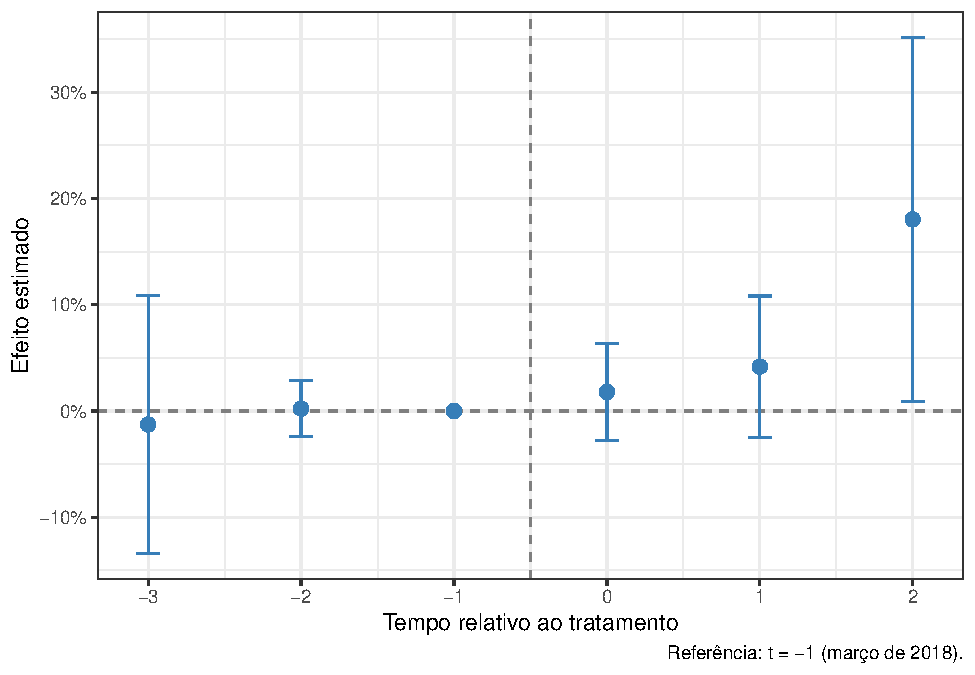
\includegraphics[keepaspectratio,alt={\label{fig:ot-event-study}Event study \textless U+2014\textgreater{} Obra Transparente. Barras indicam intervalos de 95\%, com erros-padr\textless U+00E3\textgreater o clusterizados por munic\textless U+00ED\textgreater pio.}]{bookdownproj_files/figure-latex/ot-event-study-1.pdf}}
\caption{\label{fig:ot-event-study}Event study \textless U+2014\textgreater{} Obra Transparente. Barras indicam intervalos de 95\%, com erros-padr\textless U+00E3\textgreater o clusterizados por munic\textless U+00ED\textgreater pio.}
\end{figure}

Os coeficientes pré-tratamento são próximos de zero e estatisticamente insignificantes, o que é consistente com tendências paralelas. Os coeficientes pós-tratamento crescem ao longo do tempo: o efeito é pequeno no início, aumenta em 2019 e chega a cerca de 18 pontos percentuais em outubro de 2023. Como esse último intervalo atravessa a pandemia, a interpretação substantiva deve ser cautelosa.

\subsubsection{Inferência na aplicação}\label{inferuxeancia-na-aplicauxe7uxe3o}

No Obra Transparente, a política é atribuída no nível municipal. Por isso, tanto o modelo estático quanto o event study clusterizam os erros-padrão por município. A base tem muitas obras, mas apenas 21 municípios tratados; o número relevante para inferência é o número de clusters tratados, não o número de linhas do banco.

O paper trata esse problema com wild cluster bootstrap e inferência por permutação. A tabela abaixo mostra que o ATT estático permanece significativo sob wild bootstrap. O efeito dinâmico em \(t=+2\) fica no limite convencional de 5\%, e a permutação para o ATT estático é mais cautelosa.

\begin{Shaded}
\begin{Highlighting}[]
\NormalTok{wild\_results }\SpecialCharTok{\%\textgreater{}\%}
  \FunctionTok{mutate}\NormalTok{(}
    \AttributeTok{estimate =} \FunctionTok{round}\NormalTok{(estimate, }\DecValTok{3}\NormalTok{),}
    \AttributeTok{se\_cluster =} \FunctionTok{round}\NormalTok{(se\_cluster, }\DecValTok{3}\NormalTok{),}
    \AttributeTok{p\_cluster =} \FunctionTok{round}\NormalTok{(p\_cluster, }\DecValTok{3}\NormalTok{),}
    \AttributeTok{p\_wild\_bootstrap =} \FunctionTok{round}\NormalTok{(p\_wild\_bootstrap, }\DecValTok{3}\NormalTok{),}
    \AttributeTok{p\_permutation =} \FunctionTok{round}\NormalTok{(p\_permutation, }\DecValTok{3}\NormalTok{),}
    \AttributeTok{leitura =} \FunctionTok{case\_when}\NormalTok{(}
\NormalTok{      coefficient }\SpecialCharTok{==} \StringTok{"Static ATT"} \SpecialCharTok{\textasciitilde{}} \StringTok{"ATT médio: robusto no wild bootstrap; permutação é mais cautelosa."}\NormalTok{,}
\NormalTok{      coefficient }\SpecialCharTok{==} \StringTok{"t=+2 (2023)"} \SpecialCharTok{\textasciitilde{}} \StringTok{"Maior efeito dinâmico; fica no limite de 5\% no wild bootstrap."}\NormalTok{,}
      \FunctionTok{grepl}\NormalTok{(}\StringTok{"\^{}t={-}"}\NormalTok{, coefficient) }\SpecialCharTok{\textasciitilde{}} \StringTok{"Diagnóstico pré{-}tratamento: próximo de zero."}\NormalTok{,}
      \ConstantTok{TRUE} \SpecialCharTok{\textasciitilde{}} \StringTok{"Efeito pós{-}tratamento intermediário."}
\NormalTok{    )}
\NormalTok{  ) }\SpecialCharTok{\%\textgreater{}\%}
\NormalTok{  dplyr}\SpecialCharTok{::}\FunctionTok{select}\NormalTok{(}
\NormalTok{    coefficient,}
\NormalTok{    estimate,}
\NormalTok{    se\_cluster,}
\NormalTok{    p\_cluster,}
\NormalTok{    p\_wild\_bootstrap,}
\NormalTok{    p\_permutation,}
\NormalTok{    leitura}
\NormalTok{  ) }\SpecialCharTok{\%\textgreater{}\%}
  \FunctionTok{kable}\NormalTok{(}
    \AttributeTok{caption =} \StringTok{"Inferência com poucos clusters tratados — Obra Transparente"}\NormalTok{,}
    \AttributeTok{col.names =} \FunctionTok{c}\NormalTok{(}\StringTok{"Coeficiente"}\NormalTok{, }\StringTok{"Estimativa"}\NormalTok{, }\StringTok{"SE cluster"}\NormalTok{, }\StringTok{"p cluster"}\NormalTok{, }\StringTok{"p wild"}\NormalTok{, }\StringTok{"p permutação"}\NormalTok{, }\StringTok{"Leitura"}\NormalTok{)}
\NormalTok{  )}
\end{Highlighting}
\end{Shaded}

\begin{table}

\caption{\label{tab:ot-wild-bootstrap}Inferência com poucos clusters tratados — Obra Transparente}
\centering
\begin{tabular}[t]{l|r|r|r|r|r|l}
\hline
Coeficiente & Estimativa & SE cluster & p cluster & p wild & p permutação & Leitura\\
\hline
Static ATT & 0.083 & 0.034 & 0.013 & 0.017 & 0.073 & ATT médio: robusto no wild bootstrap; permutação é mais cautelosa.\\
\hline
t=-3 (2015) & -0.013 & 0.062 & 0.837 & 0.863 & NA & Diagnóstico pré-tratamento: próximo de zero.\\
\hline
t=-2 (2017) & 0.002 & 0.013 & 0.871 & 0.901 & NA & Diagnóstico pré-tratamento: próximo de zero.\\
\hline
t=0 (Set/18) & 0.018 & 0.023 & 0.444 & 0.461 & NA & Efeito pós-tratamento intermediário.\\
\hline
t=+1 (2019) & 0.042 & 0.034 & 0.219 & 0.190 & NA & Efeito pós-tratamento intermediário.\\
\hline
t=+2 (2023) & 0.180 & 0.087 & 0.039 & 0.050 & NA & Maior efeito dinâmico; fica no limite de 5\% no wild bootstrap.\\
\hline
\end{tabular}
\end{table}

\subsubsection{Contaminação em event studies escalonados}\label{contaminauxe7uxe3o-em-event-studies-escalonados}

O gráfico de event study acima é simples porque há um único momento de adoção. Com adoção escalonada, a interpretação dos coeficientes dinâmicos de TWFE fica mais delicada. Há dois problemas distintos:

\begin{enumerate}
\def\labelenumi{\arabic{enumi}.}
\tightlist
\item
  \textbf{Pesos negativos no efeito agregado:} o coeficiente estático de TWFE pode comparar unidades tratadas cedo com unidades tratadas tarde, inclusive usando unidades já tratadas como controles.
\item
  \textbf{Contaminação dos leads e lags:} no event study dinâmico, um coeficiente de pré-tratamento pode carregar informação de efeitos pós-tratamento de outras coortes, e um coeficiente pós-tratamento pode misturar horizontes diferentes.
\end{enumerate}

Sun and Abraham (\citeproc{ref-sunabraham2021}{2021}) mostram que, quando a trajetória dinâmica do efeito varia entre coortes, os coeficientes de leads/lags do TWFE tradicional não têm interpretação limpa como efeitos em tempo relativo. Isso é particularmente perigoso porque o problema pode contaminar até o ``teste'' de pré-tendências: um coeficiente aparentemente pré-tratamento pode refletir efeitos já realizados em outra coorte. A solução é estimar efeitos específicos por coorte e tempo relativo e depois agregar com pesos explícitos, como faz o estimador \texttt{sunab()} no \texttt{fixest}.

Esse ponto é pedagógico e prático: em desenhos escalonados, não basta trocar um modelo estático por um event study. O event study também precisa usar comparações limpas.

\subsection{O problema do TWFE com tratamento escalonado}\label{o-problema-do-twfe-com-tratamento-escalonado}

Até aqui, trabalhamos com cenários em que todas as unidades tratadas recebem o tratamento ao mesmo tempo. Contudo, em muitas aplicações, o tratamento é adotado em momentos diferentes (\emph{staggered adoption}). Exemplos em ciência política incluem a adoção escalonada de biometria eleitoral, leis de transparência pública, ou reformas educacionais por diferentes estados.

Nesta seção, mostramos que o estimador TWFE pode produzir resultados enviesados --- e até com sinal trocado --- quando o tratamento é escalonado e os efeitos são heterogêneos (\citeproc{ref-dechaisemartin2020}{Chaisemartin and D'Haultfœuille 2020}, \citeproc{ref-dechaisemartin2023}{2023}).

\subsubsection{O que pode dar errado}\label{o-que-pode-dar-errado}

Considere três grupos de unidades: o grupo A (tratado no período 3), o grupo B (tratado no período 6), e o grupo C (nunca tratado). O TWFE com efeitos fixos de unidade e tempo estima um coeficiente único \(\hat{\tau}\) como uma média ponderada de todas as comparações 2×2 possíveis. Crucialmente, algumas dessas comparações usam unidades \textbf{já tratadas} como ``controle'' --- por exemplo, ao estimar o efeito para o grupo B (tratado no período 6), o TWFE pode usar o grupo A (já tratado desde o período 3) como controle.

Se o efeito do tratamento varia ao longo do tempo ou entre grupos, essas comparações ``proibidas'' introduzem viés. Em casos extremos, os pesos de algumas comparações podem ser \textbf{negativos}, fazendo com que \(\hat{\tau}\) tenha sinal oposto ao verdadeiro efeito causal.

\subsubsection{Decomposição de Goodman-Bacon --- simulação}\label{decomposiuxe7uxe3o-de-goodman-bacon-simulauxe7uxe3o}

Goodman-Bacon (\citeproc{ref-goodmanbacon2021}{2021}) mostrou que o estimador TWFE com tratamento escalonado é uma média ponderada de todos os estimadores DiD 2×2 possíveis, com pesos que dependem do tamanho dos grupos e da variância do tratamento. Vamos demonstrar isso com uma simulação.

\begin{Shaded}
\begin{Highlighting}[]
\FunctionTok{set.seed}\NormalTok{(}\DecValTok{42}\NormalTok{)}

\CommentTok{\# Parâmetros}
\NormalTok{n\_units }\OtherTok{\textless{}{-}} \DecValTok{300}
\NormalTok{n\_periods }\OtherTok{\textless{}{-}} \DecValTok{10}
\NormalTok{n\_per\_group }\OtherTok{\textless{}{-}} \DecValTok{100}

\CommentTok{\# Criar dados}
\NormalTok{sim\_data }\OtherTok{\textless{}{-}} \FunctionTok{expand.grid}\NormalTok{(}\AttributeTok{i =} \DecValTok{1}\SpecialCharTok{:}\NormalTok{n\_units, }\AttributeTok{t =} \DecValTok{1}\SpecialCharTok{:}\NormalTok{n\_periods)}

\CommentTok{\# Atribuir grupos: A (tratado em t=3), B (tratado em t=6), C (nunca tratado)}
\NormalTok{sim\_data}\SpecialCharTok{$}\NormalTok{group }\OtherTok{\textless{}{-}} \FunctionTok{ifelse}\NormalTok{(sim\_data}\SpecialCharTok{$}\NormalTok{i }\SpecialCharTok{\textless{}=}\NormalTok{ n\_per\_group, }\StringTok{"A"}\NormalTok{,}
                  \FunctionTok{ifelse}\NormalTok{(sim\_data}\SpecialCharTok{$}\NormalTok{i }\SpecialCharTok{\textless{}=} \DecValTok{2} \SpecialCharTok{*}\NormalTok{ n\_per\_group, }\StringTok{"B"}\NormalTok{, }\StringTok{"C"}\NormalTok{))}
\NormalTok{sim\_data}\SpecialCharTok{$}\NormalTok{G\_i }\OtherTok{\textless{}{-}} \FunctionTok{ifelse}\NormalTok{(sim\_data}\SpecialCharTok{$}\NormalTok{group }\SpecialCharTok{==} \StringTok{"A"}\NormalTok{, }\DecValTok{3}\NormalTok{,}
                \FunctionTok{ifelse}\NormalTok{(sim\_data}\SpecialCharTok{$}\NormalTok{group }\SpecialCharTok{==} \StringTok{"B"}\NormalTok{, }\DecValTok{6}\NormalTok{, }\ConstantTok{Inf}\NormalTok{))}

\CommentTok{\# Tratamento: D\_it = 1 se t \textgreater{}= G\_i}
\NormalTok{sim\_data}\SpecialCharTok{$}\NormalTok{D\_it }\OtherTok{\textless{}{-}} \FunctionTok{as.integer}\NormalTok{(sim\_data}\SpecialCharTok{$}\NormalTok{t }\SpecialCharTok{\textgreater{}=}\NormalTok{ sim\_data}\SpecialCharTok{$}\NormalTok{G\_i)}

\CommentTok{\# Efeito fixo de unidade}
\NormalTok{alpha\_i }\OtherTok{\textless{}{-}} \FunctionTok{rnorm}\NormalTok{(n\_units, }\AttributeTok{mean =} \DecValTok{0}\NormalTok{, }\AttributeTok{sd =} \DecValTok{2}\NormalTok{)}
\NormalTok{sim\_data}\SpecialCharTok{$}\NormalTok{alpha }\OtherTok{\textless{}{-}}\NormalTok{ alpha\_i[sim\_data}\SpecialCharTok{$}\NormalTok{i]}

\CommentTok{\# Efeito fixo de tempo}
\NormalTok{lambda\_t }\OtherTok{\textless{}{-}} \FunctionTok{seq}\NormalTok{(}\DecValTok{0}\NormalTok{, }\FloatTok{4.5}\NormalTok{, }\AttributeTok{length.out =}\NormalTok{ n\_periods)}
\NormalTok{sim\_data}\SpecialCharTok{$}\NormalTok{lambda }\OtherTok{\textless{}{-}}\NormalTok{ lambda\_t[sim\_data}\SpecialCharTok{$}\NormalTok{t]}

\CommentTok{\# Efeito causal HETEROGÊNEO: cresce com a duração do tratamento}
\CommentTok{\# Grupo A: efeito de 2 por período de exposição}
\CommentTok{\# Grupo B: efeito de 5 por período de exposição}
\NormalTok{sim\_data}\SpecialCharTok{$}\NormalTok{tau\_true }\OtherTok{\textless{}{-}} \FunctionTok{ifelse}\NormalTok{(sim\_data}\SpecialCharTok{$}\NormalTok{D\_it }\SpecialCharTok{==} \DecValTok{0}\NormalTok{, }\DecValTok{0}\NormalTok{,}
                     \FunctionTok{ifelse}\NormalTok{(sim\_data}\SpecialCharTok{$}\NormalTok{group }\SpecialCharTok{==} \StringTok{"A"}\NormalTok{,}
                            \DecValTok{2} \SpecialCharTok{*}\NormalTok{ (sim\_data}\SpecialCharTok{$}\NormalTok{t }\SpecialCharTok{{-}}\NormalTok{ sim\_data}\SpecialCharTok{$}\NormalTok{G\_i }\SpecialCharTok{+} \DecValTok{1}\NormalTok{),}
                            \DecValTok{5} \SpecialCharTok{*}\NormalTok{ (sim\_data}\SpecialCharTok{$}\NormalTok{t }\SpecialCharTok{{-}}\NormalTok{ sim\_data}\SpecialCharTok{$}\NormalTok{G\_i }\SpecialCharTok{+} \DecValTok{1}\NormalTok{)))}

\CommentTok{\# Resultado observado}
\NormalTok{sim\_data}\SpecialCharTok{$}\NormalTok{Y }\OtherTok{\textless{}{-}}\NormalTok{ sim\_data}\SpecialCharTok{$}\NormalTok{alpha }\SpecialCharTok{+}\NormalTok{ sim\_data}\SpecialCharTok{$}\NormalTok{lambda }\SpecialCharTok{+}\NormalTok{ sim\_data}\SpecialCharTok{$}\NormalTok{tau\_true }\SpecialCharTok{+} \FunctionTok{rnorm}\NormalTok{(}\FunctionTok{nrow}\NormalTok{(sim\_data))}

\CommentTok{\# ATT verdadeiro (média dos efeitos causais entre os tratados)}
\NormalTok{att\_verdadeiro }\OtherTok{\textless{}{-}} \FunctionTok{mean}\NormalTok{(sim\_data}\SpecialCharTok{$}\NormalTok{tau\_true[sim\_data}\SpecialCharTok{$}\NormalTok{D\_it }\SpecialCharTok{==} \DecValTok{1}\NormalTok{])}
\FunctionTok{cat}\NormalTok{(}\StringTok{"ATT verdadeiro:"}\NormalTok{, }\FunctionTok{round}\NormalTok{(att\_verdadeiro, }\DecValTok{2}\NormalTok{), }\StringTok{"}\SpecialCharTok{\textbackslash{}n}\StringTok{"}\NormalTok{)}
\end{Highlighting}
\end{Shaded}

\begin{verbatim}
## ATT verdadeiro: 11.31
\end{verbatim}

Agora estimamos o TWFE e comparamos com o ATT verdadeiro:

\begin{Shaded}
\begin{Highlighting}[]
\CommentTok{\# TWFE padrão}
\NormalTok{twfe\_stag }\OtherTok{\textless{}{-}} \FunctionTok{feols}\NormalTok{(Y }\SpecialCharTok{\textasciitilde{}}\NormalTok{ D\_it }\SpecialCharTok{|}\NormalTok{ i }\SpecialCharTok{+}\NormalTok{ t, }\AttributeTok{data =}\NormalTok{ sim\_data)}

\FunctionTok{cat}\NormalTok{(}\StringTok{"TWFE estimado:"}\NormalTok{, }\FunctionTok{round}\NormalTok{(}\FunctionTok{coef}\NormalTok{(twfe\_stag)[}\StringTok{"D\_it"}\NormalTok{], }\DecValTok{2}\NormalTok{), }\StringTok{"}\SpecialCharTok{\textbackslash{}n}\StringTok{"}\NormalTok{)}
\end{Highlighting}
\end{Shaded}

\begin{verbatim}
## TWFE estimado: 10.48
\end{verbatim}

\begin{Shaded}
\begin{Highlighting}[]
\FunctionTok{cat}\NormalTok{(}\StringTok{"ATT verdadeiro:"}\NormalTok{, }\FunctionTok{round}\NormalTok{(att\_verdadeiro, }\DecValTok{2}\NormalTok{), }\StringTok{"}\SpecialCharTok{\textbackslash{}n}\StringTok{"}\NormalTok{)}
\end{Highlighting}
\end{Shaded}

\begin{verbatim}
## ATT verdadeiro: 11.31
\end{verbatim}

\begin{Shaded}
\begin{Highlighting}[]
\FunctionTok{cat}\NormalTok{(}\StringTok{"Viés:"}\NormalTok{, }\FunctionTok{round}\NormalTok{(}\FunctionTok{coef}\NormalTok{(twfe\_stag)[}\StringTok{"D\_it"}\NormalTok{] }\SpecialCharTok{{-}}\NormalTok{ att\_verdadeiro, }\DecValTok{2}\NormalTok{), }\StringTok{"}\SpecialCharTok{\textbackslash{}n}\StringTok{"}\NormalTok{)}
\end{Highlighting}
\end{Shaded}

\begin{verbatim}
## Viés: -0.82
\end{verbatim}

O TWFE subestima o ATT verdadeiro. Para entender por quê, vamos decompor manualmente as comparações 2×2 que o TWFE combina.

\begin{Shaded}
\begin{Highlighting}[]
\CommentTok{\# Função auxiliar para DiD 2×2}
\NormalTok{did\_2x2 }\OtherTok{\textless{}{-}} \ControlFlowTok{function}\NormalTok{(data, treat\_group, control\_group, pre\_periods, post\_periods) \{}
\NormalTok{  d }\OtherTok{\textless{}{-}}\NormalTok{ data }\SpecialCharTok{\%\textgreater{}\%}
    \FunctionTok{filter}\NormalTok{(group }\SpecialCharTok{\%in\%} \FunctionTok{c}\NormalTok{(treat\_group, control\_group),}
\NormalTok{           t }\SpecialCharTok{\%in\%} \FunctionTok{c}\NormalTok{(pre\_periods, post\_periods)) }\SpecialCharTok{\%\textgreater{}\%}
    \FunctionTok{mutate}\NormalTok{(}\AttributeTok{post =} \FunctionTok{as.integer}\NormalTok{(t }\SpecialCharTok{\%in\%}\NormalTok{ post\_periods),}
           \AttributeTok{treated =} \FunctionTok{as.integer}\NormalTok{(group }\SpecialCharTok{==}\NormalTok{ treat\_group))}
\NormalTok{  fit }\OtherTok{\textless{}{-}} \FunctionTok{lm}\NormalTok{(Y }\SpecialCharTok{\textasciitilde{}}\NormalTok{ post }\SpecialCharTok{*}\NormalTok{ treated, }\AttributeTok{data =}\NormalTok{ d)}
  \FunctionTok{coef}\NormalTok{(fit)[}\StringTok{"post:treated"}\NormalTok{]}
\NormalTok{\}}

\CommentTok{\# Comparações possíveis:}
\CommentTok{\# 1. Grupo A (tratado t=3) vs. Grupo C (nunca tratado)}
\NormalTok{did\_AC }\OtherTok{\textless{}{-}} \FunctionTok{did\_2x2}\NormalTok{(sim\_data, }\StringTok{"A"}\NormalTok{, }\StringTok{"C"}\NormalTok{, }\AttributeTok{pre\_periods =} \DecValTok{1}\SpecialCharTok{:}\DecValTok{2}\NormalTok{, }\AttributeTok{post\_periods =} \DecValTok{3}\SpecialCharTok{:}\DecValTok{10}\NormalTok{)}

\CommentTok{\# 2. Grupo B (tratado t=6) vs. Grupo C (nunca tratado)}
\NormalTok{did\_BC }\OtherTok{\textless{}{-}} \FunctionTok{did\_2x2}\NormalTok{(sim\_data, }\StringTok{"B"}\NormalTok{, }\StringTok{"C"}\NormalTok{, }\AttributeTok{pre\_periods =} \DecValTok{1}\SpecialCharTok{:}\DecValTok{5}\NormalTok{, }\AttributeTok{post\_periods =} \DecValTok{6}\SpecialCharTok{:}\DecValTok{10}\NormalTok{)}

\CommentTok{\# 3. Grupo A (early) vs. Grupo B (late) — B como controle, pré t\textless{}3}
\NormalTok{did\_AB\_early }\OtherTok{\textless{}{-}} \FunctionTok{did\_2x2}\NormalTok{(sim\_data, }\StringTok{"A"}\NormalTok{, }\StringTok{"B"}\NormalTok{, }\AttributeTok{pre\_periods =} \DecValTok{1}\SpecialCharTok{:}\DecValTok{2}\NormalTok{, }\AttributeTok{post\_periods =} \DecValTok{3}\SpecialCharTok{:}\DecValTok{5}\NormalTok{)}

\CommentTok{\# 4. Grupo B (late) vs. Grupo A (early, já tratado!) — A como "controle"}
\NormalTok{did\_BA\_late }\OtherTok{\textless{}{-}} \FunctionTok{did\_2x2}\NormalTok{(sim\_data, }\StringTok{"B"}\NormalTok{, }\StringTok{"A"}\NormalTok{, }\AttributeTok{pre\_periods =} \DecValTok{3}\SpecialCharTok{:}\DecValTok{5}\NormalTok{, }\AttributeTok{post\_periods =} \DecValTok{6}\SpecialCharTok{:}\DecValTok{10}\NormalTok{)}

\NormalTok{comparacoes }\OtherTok{\textless{}{-}} \FunctionTok{data.frame}\NormalTok{(}
  \AttributeTok{Comparacao =} \FunctionTok{c}\NormalTok{(}\StringTok{"A vs. C (nunca tratado)"}\NormalTok{,}
                 \StringTok{"B vs. C (nunca tratado)"}\NormalTok{,}
                 \StringTok{"A vs. B (B ainda não tratado)"}\NormalTok{,}
                 \StringTok{"B vs. A (A já tratado!)"}\NormalTok{),}
  \AttributeTok{DiD\_2x2 =} \FunctionTok{round}\NormalTok{(}\FunctionTok{c}\NormalTok{(did\_AC, did\_BC, did\_AB\_early, did\_BA\_late), }\DecValTok{2}\NormalTok{)}
\NormalTok{)}

\FunctionTok{kable}\NormalTok{(comparacoes, }\AttributeTok{caption =} \StringTok{"Decomposição das comparações 2×2 no TWFE"}\NormalTok{,}
      \AttributeTok{col.names =} \FunctionTok{c}\NormalTok{(}\StringTok{"Comparação"}\NormalTok{, }\StringTok{"Estimativa DiD 2×2"}\NormalTok{))}
\end{Highlighting}
\end{Shaded}

\begin{table}

\caption{\label{tab:bacon-decomp-manual}Decomposição das comparações 2×2 no TWFE}
\centering
\begin{tabular}[t]{l|r}
\hline
Comparação & Estimativa DiD 2×2\\
\hline
A vs. C (nunca tratado) & 9.12\\
\hline
B vs. C (nunca tratado) & 15.02\\
\hline
A vs. B (B ainda não tratado) & 3.94\\
\hline
B vs. A (A já tratado!) & 7.00\\
\hline
\end{tabular}
\end{table}

A última comparação (B vs.~A, com A já tratado) é problemática: o grupo A continua acumulando efeitos do tratamento, então sua trajetória como ``controle'' viola a lógica do DiD. Se o efeito de A está crescendo, essa comparação subestima o efeito de B.

\begin{figure}
\centering
\pandocbounded{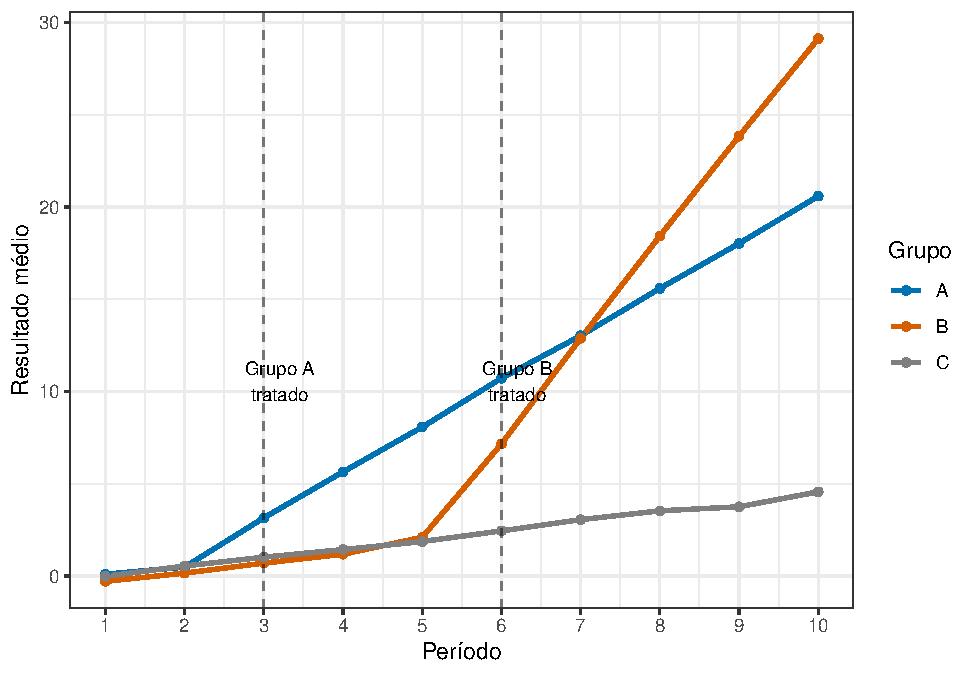
\includegraphics[keepaspectratio,alt={\label{fig:bacon-grafico}M\textless U+00E9\textgreater dias por grupo ao longo do tempo. As linhas verticais indicam o in\textless U+00ED\textgreater cio do tratamento para cada grupo. Note como o grupo A (j\textless U+00E1\textgreater{} tratado) continua mudando ap\textless U+00F3\textgreater s o per\textless U+00ED\textgreater odo 3 \textless U+2014\textgreater{} us\textless U+00E1\textgreater-lo como controle para B \textless U+00E9\textgreater{} problem\textless U+00E1\textgreater tico.}]{bookdownproj_files/figure-latex/bacon-grafico-1.pdf}}
\caption{\label{fig:bacon-grafico}M\textless U+00E9\textgreater dias por grupo ao longo do tempo. As linhas verticais indicam o in\textless U+00ED\textgreater cio do tratamento para cada grupo. Note como o grupo A (j\textless U+00E1\textgreater{} tratado) continua mudando ap\textless U+00F3\textgreater s o per\textless U+00ED\textgreater odo 3 \textless U+2014\textgreater{} us\textless U+00E1\textgreater-lo como controle para B \textless U+00E9\textgreater{} problem\textless U+00E1\textgreater tico.}
\end{figure}

Para aplicações reais, o pacote \texttt{bacondecomp} automatiza essa decomposição e produz gráficos de diagnóstico (\citeproc{ref-goodmanbacon2021}{Goodman-Bacon 2021}). Aqui usamos a simulação para fins pedagógicos.

\subsubsection{Conexão com FWL e Gardner}\label{conexuxe3o-com-fwl-e-gardner}

Há outra forma de entender o problema do TWFE, via o teorema de Frisch-Waugh-Lovell (FWL). O TWFE estima \(\hat{\tau}\) como uma regressão de \(Y\) sobre \(D_{it}\) após remover os efeitos fixos. Pelo FWL, isso equivale a:

\textbf{Passo 1.} Residualizar \(Y\) e \(D\) nos efeitos fixos:

\[
\tilde{Y}_{it} = Y_{it} - \hat{\alpha}_i - \hat{\lambda}_t, \qquad \tilde{D}_{it} = D_{it} - \hat{\alpha}^D_i - \hat{\lambda}^D_t
\]

\textbf{Passo 2.} Regredir \(\tilde{Y}_{it}\) em \(\tilde{D}_{it}\):

\[
\hat{\tau}^{TWFE} = \frac{\sum_{i,t} \tilde{D}_{it} \tilde{Y}_{it}}{\sum_{i,t} \tilde{D}_{it}^2} = \sum_{i,t} w_{it} \cdot \tau_{it}
\]

Os pesos \(w_{it}\) dependem de \(\tilde{D}_{it}\). Para unidades tratadas cedo e observadas muito depois do tratamento, \(\tilde{D}_{it}\) pode ser \textbf{negativo} (porque a média de \(D\) para essas unidades é alta, e o resíduo fica negativo). Pesos negativos significam que o TWFE pode dar sinal oposto ao efeito verdadeiro.

A solução proposta por Gardner (\citeproc{ref-gardner2022}{2022}) é o \textbf{DiD em dois estágios}:

\begin{itemize}
\item
  \textbf{Estágio 1:} Estimar os efeitos fixos \(\hat{\alpha}_i\) e \(\hat{\lambda}_t\) usando \textbf{apenas} observações não tratadas (ou ainda não tratadas). Isso evita que o efeito do tratamento contamine as estimativas dos efeitos fixos.
\item
  \textbf{Estágio 2:} Regredir \(Y_{it} - \hat{\alpha}_i - \hat{\lambda}_t\) em \(D_{it}\) para estimar o ATT.
\end{itemize}

O pacote \texttt{did2s} implementa esse procedimento com erros-padrão corrigidos para o primeiro estágio.

\subsection{Estimadores modernos}\label{estimadores-modernos}

Nesta seção, aplicamos os estimadores modernos ao \textbf{mesmo dataset simulado} da seção anterior. Isso permite comparar diretamente cada estimador com o TWFE enviesado e com o ATT verdadeiro.

\subsubsection{Callaway \& Sant'Anna}\label{callaway-santanna}

Callaway and Sant'Anna (\citeproc{ref-callawaysantanna2021}{2021}) propõem estimar o efeito para cada \textbf{grupo-tempo} \(ATT(g, t)\), onde \(g\) é o período de primeiro tratamento. A ideia é fazer comparações ``limpas'': cada grupo tratado é comparado apenas com unidades nunca tratadas (ou ainda não tratadas).

O parâmetro \(ATT(g, t) = \mathbb{E}[Y_{it}(1) - Y_{it}(0) \mid G_i = g]\) é estimado para cada combinação \((g, t)\) com \(t \geq g\). Esses efeitos grupo-tempo podem então ser \textbf{agregados} de diversas formas: por grupo, por tempo relativo (event study), ou em uma média simples.

\begin{Shaded}
\begin{Highlighting}[]
\FunctionTok{library}\NormalTok{(did)}

\CommentTok{\# Preparar dados: G\_i numérico (Inf {-}\textgreater{} 0 para nunca tratados no pacote did)}
\NormalTok{sim\_cs }\OtherTok{\textless{}{-}}\NormalTok{ sim\_data }\SpecialCharTok{\%\textgreater{}\%}
  \FunctionTok{mutate}\NormalTok{(}\AttributeTok{G\_did =} \FunctionTok{ifelse}\NormalTok{(}\FunctionTok{is.infinite}\NormalTok{(G\_i), }\DecValTok{0}\NormalTok{, G\_i))}

\CommentTok{\# Estimar ATT(g,t)}
\NormalTok{cs\_out }\OtherTok{\textless{}{-}} \FunctionTok{att\_gt}\NormalTok{(}\AttributeTok{yname =} \StringTok{"Y"}\NormalTok{,}
                 \AttributeTok{tname =} \StringTok{"t"}\NormalTok{,}
                 \AttributeTok{idname =} \StringTok{"i"}\NormalTok{,}
                 \AttributeTok{gname =} \StringTok{"G\_did"}\NormalTok{,}
                 \AttributeTok{data =}\NormalTok{ sim\_cs,}
                 \AttributeTok{control\_group =} \StringTok{"nevertreated"}\NormalTok{)}

\CommentTok{\# Agregar por tempo relativo (event study)}
\NormalTok{cs\_es }\OtherTok{\textless{}{-}} \FunctionTok{aggte}\NormalTok{(cs\_out, }\AttributeTok{type =} \StringTok{"dynamic"}\NormalTok{)}
\FunctionTok{summary}\NormalTok{(cs\_es)}
\end{Highlighting}
\end{Shaded}

\begin{verbatim}
## 
## Call:
## aggte(MP = cs_out, type = "dynamic")
## 
## Reference: Callaway, Brantly and Pedro H.C. Sant'Anna.  "Difference-in-Differences with Multiple Time Periods." Journal of Econometrics, Vol. 225, No. 2, pp. 200-230, 2021. <https://doi.org/10.1016/j.jeconom.2020.12.001>, <https://arxiv.org/abs/1803.09015> 
## 
## 
## Overall summary of ATT's based on event-study/dynamic aggregation:  
##    ATT    Std. Error     [ 95%  Conf. Int.]  
##  11.82        0.2191    11.3907     12.2493 *
## 
## 
## Dynamic Effects:
##  Event time Estimate Std. Error [95% Simult.  Conf. Band]  
##          -4  -0.1106     0.2023       -0.6570      0.4359  
##          -3   0.0616     0.1875       -0.4449      0.5681  
##          -2   0.0692     0.1763       -0.4073      0.5456  
##          -1   0.1543     0.1474       -0.2440      0.5525  
##           0   3.3379     0.1628        2.8979      3.7779 *
##           1   6.9332     0.2271        6.3195      7.5468 *
##           2  10.4648     0.3323        9.5668     11.3627 *
##           3  14.0950     0.4129       12.9794     15.2107 *
##           4  17.1856     0.5468       15.7082     18.6629 *
##           5  12.1179     0.1954       11.5899     12.6459 *
##           6  14.3349     0.1963       13.8046     14.8652 *
##           7  16.0907     0.1913       15.5738     16.6075 *
## ---
## Signif. codes: `*' confidence band does not cover 0
## 
## Control Group:  Never Treated,  Anticipation Periods:  0
## Estimation Method:  Doubly Robust
\end{verbatim}

\begin{Shaded}
\begin{Highlighting}[]
\NormalTok{cs\_plot\_data }\OtherTok{\textless{}{-}}\NormalTok{ tibble}\SpecialCharTok{::}\FunctionTok{tibble}\NormalTok{(}
  \AttributeTok{tempo\_relativo =}\NormalTok{ cs\_es}\SpecialCharTok{$}\NormalTok{egt,}
  \AttributeTok{estimativa =}\NormalTok{ cs\_es}\SpecialCharTok{$}\NormalTok{att.egt,}
  \AttributeTok{erro\_padrao =}\NormalTok{ cs\_es}\SpecialCharTok{$}\NormalTok{se.egt}
\NormalTok{) }\SpecialCharTok{\%\textgreater{}\%}
  \FunctionTok{mutate}\NormalTok{(}
    \AttributeTok{periodo =} \FunctionTok{factor}\NormalTok{(}\FunctionTok{ifelse}\NormalTok{(tempo\_relativo }\SpecialCharTok{\textless{}} \DecValTok{0}\NormalTok{, }\StringTok{"Pré"}\NormalTok{, }\StringTok{"Pós"}\NormalTok{), }\AttributeTok{levels =} \FunctionTok{c}\NormalTok{(}\StringTok{"Pré"}\NormalTok{, }\StringTok{"Pós"}\NormalTok{)),}
    \AttributeTok{ic\_inf =}\NormalTok{ estimativa }\SpecialCharTok{{-}} \FloatTok{1.96} \SpecialCharTok{*}\NormalTok{ erro\_padrao,}
    \AttributeTok{ic\_sup =}\NormalTok{ estimativa }\SpecialCharTok{+} \FloatTok{1.96} \SpecialCharTok{*}\NormalTok{ erro\_padrao}
\NormalTok{  )}

\FunctionTok{ggplot}\NormalTok{(cs\_plot\_data, }\FunctionTok{aes}\NormalTok{(}\AttributeTok{x =}\NormalTok{ tempo\_relativo, }\AttributeTok{y =}\NormalTok{ estimativa, }\AttributeTok{colour =}\NormalTok{ periodo)) }\SpecialCharTok{+}
  \FunctionTok{geom\_hline}\NormalTok{(}\AttributeTok{yintercept =} \DecValTok{0}\NormalTok{, }\AttributeTok{linetype =} \StringTok{"dashed"}\NormalTok{, }\AttributeTok{colour =} \StringTok{"grey40"}\NormalTok{) }\SpecialCharTok{+}
  \FunctionTok{geom\_vline}\NormalTok{(}\AttributeTok{xintercept =} \SpecialCharTok{{-}}\FloatTok{0.5}\NormalTok{, }\AttributeTok{linetype =} \StringTok{"dashed"}\NormalTok{, }\AttributeTok{colour =} \StringTok{"grey70"}\NormalTok{) }\SpecialCharTok{+}
  \FunctionTok{geom\_errorbar}\NormalTok{(}\FunctionTok{aes}\NormalTok{(}\AttributeTok{ymin =}\NormalTok{ ic\_inf, }\AttributeTok{ymax =}\NormalTok{ ic\_sup), }\AttributeTok{width =} \FloatTok{0.15}\NormalTok{) }\SpecialCharTok{+}
  \FunctionTok{geom\_point}\NormalTok{(}\AttributeTok{size =} \FloatTok{2.6}\NormalTok{) }\SpecialCharTok{+}
  \FunctionTok{scale\_x\_continuous}\NormalTok{(}\AttributeTok{breaks =} \FunctionTok{sort}\NormalTok{(}\FunctionTok{unique}\NormalTok{(cs\_plot\_data}\SpecialCharTok{$}\NormalTok{tempo\_relativo))) }\SpecialCharTok{+}
  \FunctionTok{scale\_colour\_manual}\NormalTok{(}\AttributeTok{values =} \FunctionTok{c}\NormalTok{(}\StringTok{"Pré"} \OtherTok{=} \StringTok{"\#D55E00"}\NormalTok{, }\StringTok{"Pós"} \OtherTok{=} \StringTok{"\#0072B2"}\NormalTok{), }\AttributeTok{name =} \ConstantTok{NULL}\NormalTok{) }\SpecialCharTok{+}
  \FunctionTok{theme\_bw}\NormalTok{() }\SpecialCharTok{+}
  \FunctionTok{labs}\NormalTok{(}
    \AttributeTok{x =} \StringTok{"Tempo relativo ao tratamento"}\NormalTok{,}
    \AttributeTok{y =} \StringTok{"Efeito estimado"}\NormalTok{,}
    \AttributeTok{caption =} \StringTok{"Estimador Callaway \& Sant\textquotesingle{}Anna; controles nunca tratados."}
\NormalTok{  ) }\SpecialCharTok{+}
  \FunctionTok{theme}\NormalTok{(}\AttributeTok{legend.position =} \StringTok{"bottom"}\NormalTok{)}
\end{Highlighting}
\end{Shaded}

\begin{figure}
\centering
\pandocbounded{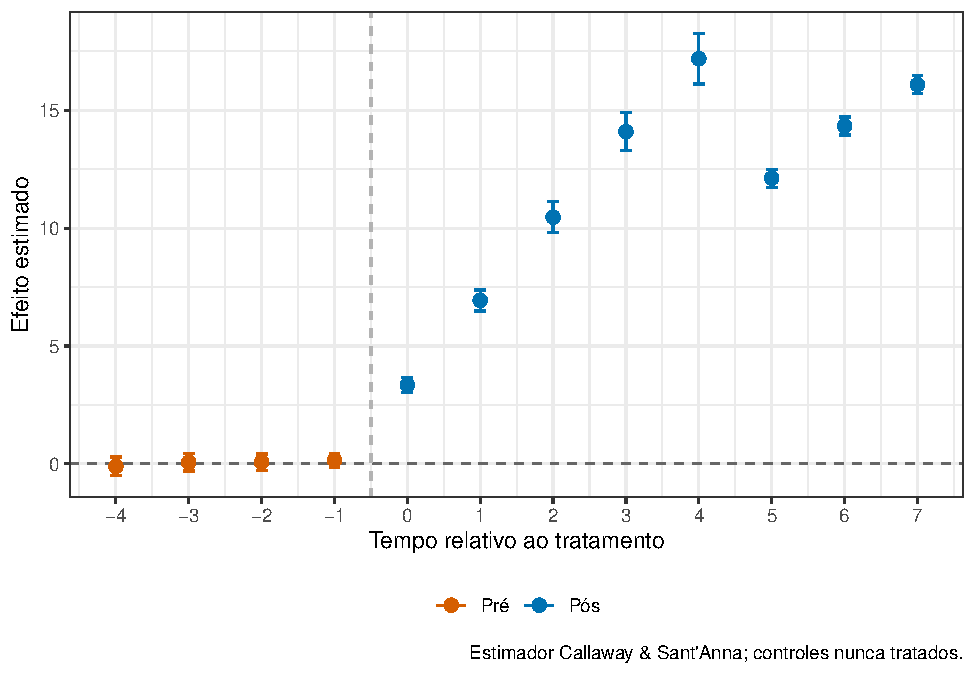
\includegraphics[keepaspectratio,alt={\label{fig:cs-estimator}Event study agregado \textless U+2014\textgreater{} Callaway \& Sant'Anna. Comparar com o TWFE da se\textless U+00E7\textgreater\textless U+00E3\textgreater o anterior.}]{bookdownproj_files/figure-latex/cs-estimator-1.pdf}}
\caption{\label{fig:cs-estimator}Event study agregado \textless U+2014\textgreater{} Callaway \& Sant'Anna. Comparar com o TWFE da se\textless U+00E7\textgreater\textless U+00E3\textgreater o anterior.}
\end{figure}

\subsubsection{Sun \& Abraham}\label{sun-abraham}

Sun and Abraham (\citeproc{ref-sunabraham2021}{2021}) propõem o \emph{interaction-weighted estimator}. A ideia é estimar coeficientes separados para cada coorte de tratamento e depois agregar com pesos adequados. O pacote \texttt{fixest} implementa isso via \texttt{sunab()}.

\begin{Shaded}
\begin{Highlighting}[]
\CommentTok{\# Preparar: nunca tratados precisam de G\_i grande (não Inf)}
\NormalTok{sim\_sa }\OtherTok{\textless{}{-}}\NormalTok{ sim\_data }\SpecialCharTok{\%\textgreater{}\%}
  \FunctionTok{mutate}\NormalTok{(}\AttributeTok{G\_sunab =} \FunctionTok{ifelse}\NormalTok{(}\FunctionTok{is.infinite}\NormalTok{(G\_i), }\DecValTok{10000}\NormalTok{, G\_i))}

\NormalTok{sa\_out }\OtherTok{\textless{}{-}} \FunctionTok{feols}\NormalTok{(Y }\SpecialCharTok{\textasciitilde{}} \FunctionTok{sunab}\NormalTok{(G\_sunab, t) }\SpecialCharTok{|}\NormalTok{ i }\SpecialCharTok{+}\NormalTok{ t, }\AttributeTok{data =}\NormalTok{ sim\_sa)}
\FunctionTok{summary}\NormalTok{(sa\_out)}
\end{Highlighting}
\end{Shaded}

\begin{verbatim}
## OLS estimation, Dep. Var.: Y
## Observations: 3,000
## Fixed-effects: i: 300,  t: 10
## Standard-errors: Clustered (i) 
##        Estimate Std. Error   t value  Pr(>|t|)    
## t::-5 -0.507467   0.195736  -2.59260 0.0099934 ** 
## t::-4 -0.618021   0.191162  -3.23298 0.0013621 ** 
## t::-3 -0.556429   0.208351  -2.67063 0.0079853 ** 
## t::-2 -0.154251   0.148310  -1.04005 0.2991553    
## t::0   3.337901   0.141628  23.56811 < 2.2e-16 ***
## t::1   6.933171   0.142400  48.68798 < 2.2e-16 ***
## t::2  10.464763   0.125684  83.26220 < 2.2e-16 ***
## t::3  14.095030   0.143729  98.06637 < 2.2e-16 ***
## t::4  17.185587   0.141087 121.80829 < 2.2e-16 ***
## t::5  12.117914   0.202001  59.98933 < 2.2e-16 ***
## t::6  14.334862   0.205640  69.70864 < 2.2e-16 ***
## t::7  16.090680   0.197595  81.43247 < 2.2e-16 ***
## ---
## Signif. codes:  0 '***' 0.001 '**' 0.01 '*' 0.05 '.' 0.1 ' ' 1
## RMSE: 0.953834     Adj. R2: 0.985194
##                  Within R2: 0.940844
\end{verbatim}

\begin{Shaded}
\begin{Highlighting}[]
\NormalTok{sa\_coef }\OtherTok{\textless{}{-}} \FunctionTok{coef}\NormalTok{(sa\_out)}
\NormalTok{sa\_se }\OtherTok{\textless{}{-}} \FunctionTok{se}\NormalTok{(sa\_out)}

\NormalTok{sa\_plot\_data }\OtherTok{\textless{}{-}}\NormalTok{ tibble}\SpecialCharTok{::}\FunctionTok{tibble}\NormalTok{(}
  \AttributeTok{tempo\_relativo =} \FunctionTok{as.integer}\NormalTok{(}\FunctionTok{sub}\NormalTok{(}\StringTok{"\^{}t::"}\NormalTok{, }\StringTok{""}\NormalTok{, }\FunctionTok{names}\NormalTok{(sa\_coef))),}
  \AttributeTok{estimativa =} \FunctionTok{as.numeric}\NormalTok{(sa\_coef),}
  \AttributeTok{erro\_padrao =} \FunctionTok{as.numeric}\NormalTok{(sa\_se)}
\NormalTok{) }\SpecialCharTok{\%\textgreater{}\%}
  \FunctionTok{bind\_rows}\NormalTok{(}
\NormalTok{    tibble}\SpecialCharTok{::}\FunctionTok{tibble}\NormalTok{(}
      \AttributeTok{tempo\_relativo =} \SpecialCharTok{{-}}\DecValTok{1}\NormalTok{,}
      \AttributeTok{estimativa =} \DecValTok{0}\NormalTok{,}
      \AttributeTok{erro\_padrao =} \ConstantTok{NA\_real\_}
\NormalTok{    )}
\NormalTok{  ) }\SpecialCharTok{\%\textgreater{}\%}
  \FunctionTok{arrange}\NormalTok{(tempo\_relativo) }\SpecialCharTok{\%\textgreater{}\%}
  \FunctionTok{mutate}\NormalTok{(}
    \AttributeTok{periodo =} \FunctionTok{factor}\NormalTok{(}\FunctionTok{ifelse}\NormalTok{(tempo\_relativo }\SpecialCharTok{\textless{}} \DecValTok{0}\NormalTok{, }\StringTok{"Pré"}\NormalTok{, }\StringTok{"Pós"}\NormalTok{), }\AttributeTok{levels =} \FunctionTok{c}\NormalTok{(}\StringTok{"Pré"}\NormalTok{, }\StringTok{"Pós"}\NormalTok{)),}
    \AttributeTok{ic\_inf =}\NormalTok{ estimativa }\SpecialCharTok{{-}} \FloatTok{1.96} \SpecialCharTok{*}\NormalTok{ erro\_padrao,}
    \AttributeTok{ic\_sup =}\NormalTok{ estimativa }\SpecialCharTok{+} \FloatTok{1.96} \SpecialCharTok{*}\NormalTok{ erro\_padrao}
\NormalTok{  )}

\FunctionTok{ggplot}\NormalTok{(sa\_plot\_data, }\FunctionTok{aes}\NormalTok{(}\AttributeTok{x =}\NormalTok{ tempo\_relativo, }\AttributeTok{y =}\NormalTok{ estimativa, }\AttributeTok{colour =}\NormalTok{ periodo)) }\SpecialCharTok{+}
  \FunctionTok{geom\_hline}\NormalTok{(}\AttributeTok{yintercept =} \DecValTok{0}\NormalTok{, }\AttributeTok{linetype =} \StringTok{"dashed"}\NormalTok{, }\AttributeTok{colour =} \StringTok{"grey40"}\NormalTok{) }\SpecialCharTok{+}
  \FunctionTok{geom\_vline}\NormalTok{(}\AttributeTok{xintercept =} \SpecialCharTok{{-}}\FloatTok{0.5}\NormalTok{, }\AttributeTok{linetype =} \StringTok{"dashed"}\NormalTok{, }\AttributeTok{colour =} \StringTok{"grey70"}\NormalTok{) }\SpecialCharTok{+}
  \FunctionTok{geom\_errorbar}\NormalTok{(}
    \AttributeTok{data =}\NormalTok{ sa\_plot\_data }\SpecialCharTok{\%\textgreater{}\%} \FunctionTok{filter}\NormalTok{(}\SpecialCharTok{!}\FunctionTok{is.na}\NormalTok{(erro\_padrao)),}
    \FunctionTok{aes}\NormalTok{(}\AttributeTok{ymin =}\NormalTok{ ic\_inf, }\AttributeTok{ymax =}\NormalTok{ ic\_sup),}
    \AttributeTok{width =} \FloatTok{0.15}
\NormalTok{  ) }\SpecialCharTok{+}
  \FunctionTok{geom\_point}\NormalTok{(}\AttributeTok{size =} \FloatTok{2.6}\NormalTok{) }\SpecialCharTok{+}
  \FunctionTok{scale\_x\_continuous}\NormalTok{(}\AttributeTok{breaks =} \FunctionTok{sort}\NormalTok{(}\FunctionTok{unique}\NormalTok{(sa\_plot\_data}\SpecialCharTok{$}\NormalTok{tempo\_relativo))) }\SpecialCharTok{+}
  \FunctionTok{scale\_colour\_manual}\NormalTok{(}\AttributeTok{values =} \FunctionTok{c}\NormalTok{(}\StringTok{"Pré"} \OtherTok{=} \StringTok{"\#D55E00"}\NormalTok{, }\StringTok{"Pós"} \OtherTok{=} \StringTok{"\#0072B2"}\NormalTok{), }\AttributeTok{name =} \ConstantTok{NULL}\NormalTok{) }\SpecialCharTok{+}
  \FunctionTok{theme\_bw}\NormalTok{() }\SpecialCharTok{+}
  \FunctionTok{labs}\NormalTok{(}
    \AttributeTok{x =} \StringTok{"Tempo relativo ao tratamento"}\NormalTok{,}
    \AttributeTok{y =} \StringTok{"Efeito estimado"}\NormalTok{,}
    \AttributeTok{caption =} \StringTok{"Estimador Sun \& Abraham; referência: t = {-}1."}
\NormalTok{  ) }\SpecialCharTok{+}
  \FunctionTok{theme}\NormalTok{(}\AttributeTok{legend.position =} \StringTok{"bottom"}\NormalTok{)}
\end{Highlighting}
\end{Shaded}

\begin{figure}
\centering
\pandocbounded{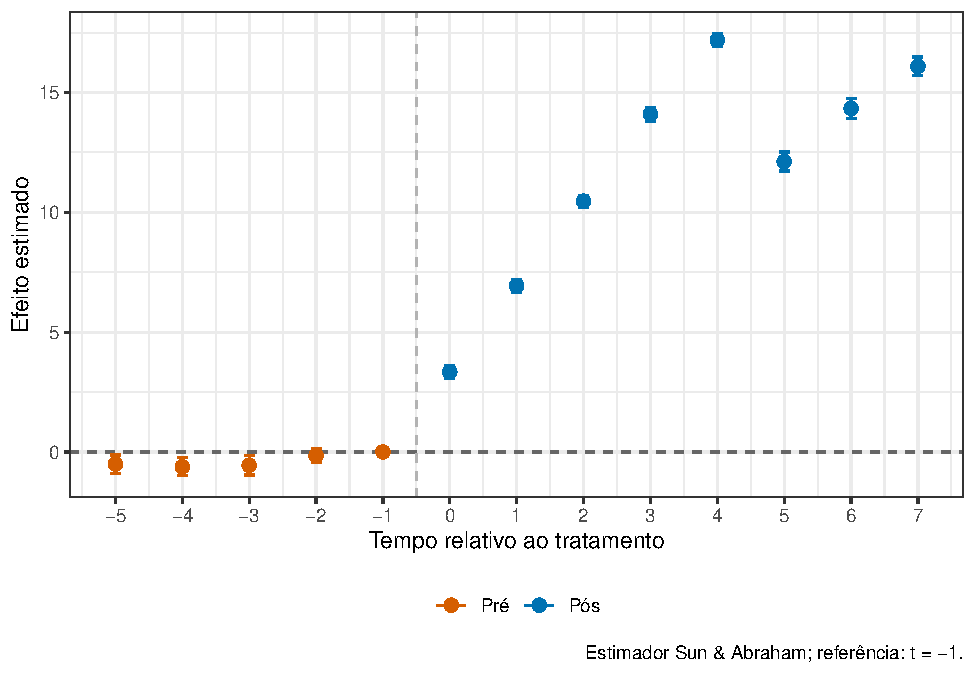
\includegraphics[keepaspectratio,alt={\label{fig:sunab-estimator}Event study \textless U+2014\textgreater{} Sun \& Abraham (sunab).}]{bookdownproj_files/figure-latex/sunab-estimator-1.pdf}}
\caption{\label{fig:sunab-estimator}Event study \textless U+2014\textgreater{} Sun \& Abraham (sunab).}
\end{figure}

\subsubsection{Gardner / did2s}\label{gardner-did2s}

O estimador de dois estágios de Gardner (\citeproc{ref-gardner2022}{2022}), discutido acima na conexão com FWL, é implementado pelo pacote \texttt{did2s}.

\begin{Shaded}
\begin{Highlighting}[]
\FunctionTok{library}\NormalTok{(did2s)}

\NormalTok{sim\_d2s }\OtherTok{\textless{}{-}}\NormalTok{ sim\_data }\SpecialCharTok{\%\textgreater{}\%}
  \FunctionTok{mutate}\NormalTok{(}\AttributeTok{first\_treat =} \FunctionTok{ifelse}\NormalTok{(}\FunctionTok{is.infinite}\NormalTok{(G\_i), }\ConstantTok{Inf}\NormalTok{, G\_i))}

\NormalTok{d2s\_out }\OtherTok{\textless{}{-}} \FunctionTok{did2s}\NormalTok{(}\AttributeTok{data =}\NormalTok{ sim\_d2s,}
                 \AttributeTok{yname =} \StringTok{"Y"}\NormalTok{,}
                 \AttributeTok{first\_stage =} \SpecialCharTok{\textasciitilde{}} \DecValTok{0} \SpecialCharTok{|}\NormalTok{ i }\SpecialCharTok{+}\NormalTok{ t,}
                 \AttributeTok{second\_stage =} \SpecialCharTok{\textasciitilde{}}\NormalTok{ D\_it,}
                 \AttributeTok{treatment =} \StringTok{"D\_it"}\NormalTok{,}
                 \AttributeTok{cluster\_var =} \StringTok{"i"}\NormalTok{)}

\FunctionTok{summary}\NormalTok{(d2s\_out)}
\end{Highlighting}
\end{Shaded}

\begin{verbatim}
## OLS estimation, Dep. Var.: Y
## Observations: 3,000
## Standard-errors: Custom 
##      Estimate Std. Error t value  Pr(>|t|)    
## D_it  11.3374   0.212622 53.3218 < 2.2e-16 ***
## ---
## Signif. codes:  0 '***' 0.001 '**' 0.01 '*' 0.05 '.' 0.1 ' ' 1
## RMSE: 4.31369   Adj. R2: 0.628984
\end{verbatim}

\subsubsection{Borusyak, Jaravel \& Spiess}\label{borusyak-jaravel-spiess}

Borusyak, Jaravel, and Spiess (\citeproc{ref-borusyak2024}{2024}) propõem um estimador por \textbf{imputação}: estimam o modelo de efeitos fixos nos dados não tratados e usam as previsões para imputar os contrafactuais das unidades tratadas. O efeito é a diferença entre o observado e o imputado.

\begin{Shaded}
\begin{Highlighting}[]
\FunctionTok{library}\NormalTok{(didimputation)}

\NormalTok{sim\_imp }\OtherTok{\textless{}{-}}\NormalTok{ sim\_data }\SpecialCharTok{\%\textgreater{}\%}
  \FunctionTok{mutate}\NormalTok{(}\AttributeTok{Ei =} \FunctionTok{ifelse}\NormalTok{(}\FunctionTok{is.infinite}\NormalTok{(G\_i), }\DecValTok{0}\NormalTok{, G\_i))}

\NormalTok{imp\_out }\OtherTok{\textless{}{-}} \FunctionTok{did\_imputation}\NormalTok{(}\AttributeTok{data =}\NormalTok{ sim\_imp,}
                          \AttributeTok{yname =} \StringTok{"Y"}\NormalTok{,}
                          \AttributeTok{gname =} \StringTok{"Ei"}\NormalTok{,}
                          \AttributeTok{tname =} \StringTok{"t"}\NormalTok{,}
                          \AttributeTok{idname =} \StringTok{"i"}\NormalTok{,}
                          \AttributeTok{first\_stage =} \SpecialCharTok{\textasciitilde{}} \DecValTok{0} \SpecialCharTok{|}\NormalTok{ i }\SpecialCharTok{+}\NormalTok{ t)}

\FunctionTok{summary}\NormalTok{(imp\_out)}
\end{Highlighting}
\end{Shaded}

\begin{verbatim}
##      lhs                term              estimate       std.error      
##  Length:1           Length:1           Min.   :11.34   Min.   :0.07615  
##  Class :character   Class :character   1st Qu.:11.34   1st Qu.:0.07615  
##  Mode  :character   Mode  :character   Median :11.34   Median :0.07615  
##                                        Mean   :11.34   Mean   :0.07615  
##                                        3rd Qu.:11.34   3rd Qu.:0.07615  
##                                        Max.   :11.34   Max.   :0.07615  
##     conf.low       conf.high    
##  Min.   :11.19   Min.   :11.49  
##  1st Qu.:11.19   1st Qu.:11.49  
##  Median :11.19   Median :11.49  
##  Mean   :11.19   Mean   :11.49  
##  3rd Qu.:11.19   3rd Qu.:11.49  
##  Max.   :11.19   Max.   :11.49
\end{verbatim}

\subsubsection{Tabela comparativa}\label{tabela-comparativa}

\begin{Shaded}
\begin{Highlighting}[]
\CommentTok{\# Extrair ATT de cada estimador}
\NormalTok{att\_twfe }\OtherTok{\textless{}{-}} \FunctionTok{coef}\NormalTok{(twfe\_stag)[}\StringTok{"D\_it"}\NormalTok{]}
\NormalTok{att\_cs }\OtherTok{\textless{}{-}} \FunctionTok{aggte}\NormalTok{(cs\_out, }\AttributeTok{type =} \StringTok{"simple"}\NormalTok{)}\SpecialCharTok{$}\NormalTok{overall.att}
\NormalTok{att\_sa }\OtherTok{\textless{}{-}} \FunctionTok{summary}\NormalTok{(sa\_out)}\SpecialCharTok{$}\NormalTok{coeftable[}\DecValTok{1}\NormalTok{, }\DecValTok{1}\NormalTok{]}
\NormalTok{att\_d2s }\OtherTok{\textless{}{-}} \FunctionTok{coef}\NormalTok{(d2s\_out)[}\StringTok{"D\_it"}\NormalTok{]}
\NormalTok{att\_imp }\OtherTok{\textless{}{-}}\NormalTok{ imp\_out}\SpecialCharTok{$}\NormalTok{estimate[}\DecValTok{1}\NormalTok{]}

\CommentTok{\# Recuperar ATT de Sun \& Abraham corretamente: média dos coeficientes pós}
\NormalTok{sa\_coefs }\OtherTok{\textless{}{-}} \FunctionTok{coef}\NormalTok{(sa\_out)}
\NormalTok{sa\_post }\OtherTok{\textless{}{-}}\NormalTok{ sa\_coefs[}\FunctionTok{grep}\NormalTok{(}\StringTok{"\^{}t::"}\NormalTok{, }\FunctionTok{names}\NormalTok{(sa\_coefs))]}
\CommentTok{\# Filtrar apenas coeficientes pós{-}tratamento (relativos \textgreater{}= 0)}
\NormalTok{sa\_post\_names }\OtherTok{\textless{}{-}} \FunctionTok{names}\NormalTok{(sa\_post)}
\NormalTok{sa\_post\_vals }\OtherTok{\textless{}{-}} \FunctionTok{as.numeric}\NormalTok{(}\FunctionTok{gsub}\NormalTok{(}\StringTok{".*::"}\NormalTok{, }\StringTok{""}\NormalTok{, sa\_post\_names))}
\NormalTok{att\_sa\_agg }\OtherTok{\textless{}{-}} \FunctionTok{mean}\NormalTok{(sa\_post[sa\_post\_vals }\SpecialCharTok{\textgreater{}=} \DecValTok{0}\NormalTok{])}

\NormalTok{tab\_comp }\OtherTok{\textless{}{-}} \FunctionTok{data.frame}\NormalTok{(}
  \AttributeTok{Estimador =} \FunctionTok{c}\NormalTok{(}\StringTok{"ATT verdadeiro"}\NormalTok{, }\StringTok{"TWFE (enviesado)"}\NormalTok{, }\StringTok{"Callaway \& Sant\textquotesingle{}Anna"}\NormalTok{,}
                \StringTok{"Sun \& Abraham"}\NormalTok{, }\StringTok{"Gardner (did2s)"}\NormalTok{, }\StringTok{"Imputação (BJS)"}\NormalTok{),}
  \AttributeTok{Ideia =} \FunctionTok{c}\NormalTok{(}
    \StringTok{"Benchmark da simulação"}\NormalTok{,}
    \StringTok{"Um coeficiente TWFE"}\NormalTok{,}
    \StringTok{"ATT(g,t) e agregação explícita"}\NormalTok{,}
    \StringTok{"Interações coorte × tempo relativo"}\NormalTok{,}
    \StringTok{"Dois estágios com FE estimados nos não tratados"}\NormalTok{,}
    \StringTok{"Imputação de Y(0) a partir dos não tratados"}
\NormalTok{  ),}
  \AttributeTok{Comparacao =} \FunctionTok{c}\NormalTok{(}
    \StringTok{"Efeito conhecido pelo DGP"}\NormalTok{,}
    \StringTok{"Mistura comparações limpas e problemáticas"}\NormalTok{,}
    \StringTok{"Tratados vs. nunca tratados"}\NormalTok{,}
    \StringTok{"Coortes comparadas com pesos explícitos"}\NormalTok{,}
    \StringTok{"Tratados vs. contrafactual residualizado"}\NormalTok{,}
    \StringTok{"Observado tratado vs. Y(0) imputado"}
\NormalTok{  ),}
  \AttributeTok{Pressuposto =} \FunctionTok{c}\NormalTok{(}
    \StringTok{"Nenhum: benchmark conhecido pelo DGP"}\NormalTok{,}
    \StringTok{"PT, sem antecipação e efeitos homogêneos para ATT limpo"}\NormalTok{,}
    \StringTok{"PT por coorte, sem antecipação e tratamento absorvente"}\NormalTok{,}
    \StringTok{"PT por coorte, sem antecipação e coortes não contaminadas"}\NormalTok{,}
    \StringTok{"Modelo FE de Y(0) nos não tratados; sem antecipação"}\NormalTok{,}
    \StringTok{"Modelo de Y(0) nos não tratados; sem antecipação"}
\NormalTok{  ),}
  \AttributeTok{ATT =} \FunctionTok{round}\NormalTok{(}\FunctionTok{c}\NormalTok{(att\_verdadeiro, att\_twfe, att\_cs, att\_sa\_agg, att\_d2s, att\_imp), }\DecValTok{2}\NormalTok{)}
\NormalTok{)}

\FunctionTok{kable}\NormalTok{(tab\_comp, }\AttributeTok{caption =} \StringTok{"Comparação dos estimadores — dados simulados com tratamento escalonado e efeitos heterogêneos"}\NormalTok{,}
      \AttributeTok{col.names =} \FunctionTok{c}\NormalTok{(}\StringTok{"Estimador"}\NormalTok{, }\StringTok{"Ideia"}\NormalTok{, }\StringTok{"Comparação usada"}\NormalTok{, }\StringTok{"Pressuposto{-}chave"}\NormalTok{, }\StringTok{"ATT estimado"}\NormalTok{))}
\end{Highlighting}
\end{Shaded}

\begin{table}

\caption{\label{tab:tabela-comparativa}Comparação dos estimadores — dados simulados com tratamento escalonado e efeitos heterogêneos}
\centering
\begin{tabular}[t]{l|l|l|l|r}
\hline
Estimador & Ideia & Comparação usada & Pressuposto-chave & ATT estimado\\
\hline
ATT verdadeiro & Benchmark da simulação & Efeito conhecido pelo DGP & Nenhum: benchmark conhecido pelo DGP & 11.31\\
\hline
TWFE (enviesado) & Um coeficiente TWFE & Mistura comparações limpas e problemáticas & PT, sem antecipação e efeitos homogêneos para ATT limpo & 10.48\\
\hline
Callaway \& Sant'Anna & ATT(g,t) e agregação explícita & Tratados vs. nunca tratados & PT por coorte, sem antecipação e tratamento absorvente & 11.28\\
\hline
Sun \& Abraham & Interações coorte × tempo relativo & Coortes comparadas com pesos explícitos & PT por coorte, sem antecipação e coortes não contaminadas & 11.82\\
\hline
Gardner (did2s) & Dois estágios com FE estimados nos não tratados & Tratados vs. contrafactual residualizado & Modelo FE de Y(0) nos não tratados; sem antecipação & 11.34\\
\hline
Imputação (BJS) & Imputação de Y(0) a partir dos não tratados & Observado tratado vs. Y(0) imputado & Modelo de Y(0) nos não tratados; sem antecipação & 11.34\\
\hline
\end{tabular}
\end{table}

A tabela mostra que o TWFE diverge do ATT verdadeiro, enquanto os estimadores modernos convergem para valores mais próximos do efeito real. A coluna de pressupostos destaca a exigência distintiva de cada estimador, não uma lista completa: todos continuam exigindo ausência de spillovers relevantes, boa mensuração do tratamento e do outcome, e composição comparável ao longo do tempo. Tratamento absorvente significa ``sem on/off'': depois de tratada, a unidade permanece tratada. As pequenas diferenças entre os estimadores modernos decorrem de diferenças nos esquemas de ponderação e na definição exata do estimando.

\subsection{Testando tendências paralelas e análise de sensibilidade}\label{testando-tenduxeancias-paralelas-e-anuxe1lise-de-sensibilidade}

\subsubsection{Pré-tendências e o aviso de Roth}\label{pruxe9-tenduxeancias-e-o-aviso-de-roth}

O event study é a ferramenta padrão para avaliar a plausibilidade de tendências paralelas: se os coeficientes pré-tratamento (\(\delta_k\) para \(k < 0\)) são próximos de zero, isso é consistente com PT. Porém, Roth (\citeproc{ref-roth2022}{2022}) alerta para o \textbf{viés de pré-teste} (\emph{pre-testing bias}): se selecionamos especificações ou amostras com base em pré-tendências insignificantes, podemos estar condicionando em ruído favorável, o que infla os coeficientes pós-tratamento.

Em outras palavras, a ausência de pré-tendências significativas é necessária mas não suficiente. Roth (\citeproc{ref-roth2022}{2022}) mostra que testes de pré-tendências têm baixo poder em muitas aplicações típicas --- não rejeitar PT não significa que PT é verdadeira.

\subsubsection{HonestDiD: análise de sensibilidade}\label{honestdid-anuxe1lise-de-sensibilidade}

Rambachan and Roth (\citeproc{ref-rambachanroth2023}{2023}) propõem uma abordagem de \textbf{identificação parcial}: em vez de supor PT exata, impõem restrições sobre \emph{quanto} as tendências pós-tratamento podem divergir das tendências pré-tratamento. O parâmetro \(\bar{M}\) controla essa divergência:

\begin{itemize}
\tightlist
\item
  \(\bar{M} = 0\): tendências paralelas exatas (identificação pontual).
\item
  \(\bar{M} = 1\): o desvio pós-tratamento pode ser igual ao máximo desvio observado no pré-tratamento.
\item
  \(\bar{M} = 2\): o desvio pode ser até duas vezes maior.
\end{itemize}

Vamos aplicar o HonestDiD ao event study da Obra Transparente. Esta é uma análise didática de sensibilidade: o paper principal reporta cluster municipal, wild cluster bootstrap e permutação; aqui perguntamos quanto a conclusão dinâmica depende de PT exata.

\begin{Shaded}
\begin{Highlighting}[]
\FunctionTok{library}\NormalTok{(HonestDiD)}

\ControlFlowTok{if}\NormalTok{ (}\SpecialCharTok{!}\FunctionTok{exists}\NormalTok{(}\StringTok{"did\_ot\_event"}\NormalTok{)) \{}
\NormalTok{  did\_panel }\OtherTok{\textless{}{-}} \FunctionTok{readRDS}\NormalTok{(ot\_panel\_file) }\SpecialCharTok{\%\textgreater{}\%}
    \FunctionTok{mutate}\NormalTok{(}
      \AttributeTok{treat\_m3 =}\NormalTok{ group\_treated }\SpecialCharTok{*}\NormalTok{ (rel\_time }\SpecialCharTok{==} \SpecialCharTok{{-}}\DecValTok{3}\NormalTok{),}
      \AttributeTok{treat\_m2 =}\NormalTok{ group\_treated }\SpecialCharTok{*}\NormalTok{ (rel\_time }\SpecialCharTok{==} \SpecialCharTok{{-}}\DecValTok{2}\NormalTok{),}
      \AttributeTok{treat\_0  =}\NormalTok{ group\_treated }\SpecialCharTok{*}\NormalTok{ (rel\_time }\SpecialCharTok{==} \DecValTok{0}\NormalTok{),}
      \AttributeTok{treat\_p1 =}\NormalTok{ group\_treated }\SpecialCharTok{*}\NormalTok{ (rel\_time }\SpecialCharTok{==} \DecValTok{1}\NormalTok{),}
      \AttributeTok{treat\_p2 =}\NormalTok{ group\_treated }\SpecialCharTok{*}\NormalTok{ (rel\_time }\SpecialCharTok{==} \DecValTok{2}\NormalTok{)}
\NormalTok{    )}

\NormalTok{  did\_ot\_event }\OtherTok{\textless{}{-}} \FunctionTok{feols}\NormalTok{(}
\NormalTok{    concluida }\SpecialCharTok{\textasciitilde{}}\NormalTok{ treat\_m3 }\SpecialCharTok{+}\NormalTok{ treat\_m2 }\SpecialCharTok{+}\NormalTok{ treat\_0 }\SpecialCharTok{+}\NormalTok{ treat\_p1 }\SpecialCharTok{+}\NormalTok{ treat\_p2 }\SpecialCharTok{|}\NormalTok{ id }\SpecialCharTok{+}\NormalTok{ periodo,}
    \AttributeTok{data =}\NormalTok{ did\_panel,}
    \AttributeTok{cluster =} \SpecialCharTok{\textasciitilde{}}\NormalTok{municipio}
\NormalTok{  )}
\NormalTok{\}}

\NormalTok{betahat }\OtherTok{\textless{}{-}} \FunctionTok{coef}\NormalTok{(did\_ot\_event)}
\NormalTok{sigma }\OtherTok{\textless{}{-}} \FunctionTok{vcov}\NormalTok{(did\_ot\_event)}

\CommentTok{\# Pré: t={-}3 e t={-}2; referência: t={-}1; pós: t=0, t=+1 e t=+2}
\NormalTok{numPrePeriods }\OtherTok{\textless{}{-}} \DecValTok{2}
\NormalTok{numPostPeriods }\OtherTok{\textless{}{-}} \DecValTok{3}

\NormalTok{delta\_rm\_results }\OtherTok{\textless{}{-}} \FunctionTok{createSensitivityResults\_relativeMagnitudes}\NormalTok{(}
  \AttributeTok{betahat =}\NormalTok{ betahat,}
  \AttributeTok{sigma =}\NormalTok{ sigma,}
  \AttributeTok{numPrePeriods =}\NormalTok{ numPrePeriods,}
  \AttributeTok{numPostPeriods =}\NormalTok{ numPostPeriods,}
  \AttributeTok{Mbarvec =} \FunctionTok{seq}\NormalTok{(}\FloatTok{0.5}\NormalTok{, }\DecValTok{2}\NormalTok{, }\AttributeTok{by =} \FloatTok{0.5}\NormalTok{)}
\NormalTok{)}

\NormalTok{delta\_rm\_results }\SpecialCharTok{\%\textgreater{}\%}
  \FunctionTok{kable}\NormalTok{(}
    \AttributeTok{caption =} \StringTok{"Análise de sensibilidade HonestDiD — Obra Transparente"}\NormalTok{,}
    \AttributeTok{digits =} \DecValTok{3}
\NormalTok{  )}
\end{Highlighting}
\end{Shaded}

\begin{table}

\caption{\label{tab:honestdid}Análise de sensibilidade HonestDiD — Obra Transparente}
\centering
\begin{tabular}[t]{r|r|l|l|r}
\hline
lb & ub & method & Delta & Mbar\\
\hline
-0.058 & 0.090 & C-LF & DeltaRM & 0.5\\
\hline
-0.104 & 0.136 & C-LF & DeltaRM & 1.0\\
\hline
-0.158 & 0.189 & C-LF & DeltaRM & 1.5\\
\hline
-0.213 & 0.245 & C-LF & DeltaRM & 2.0\\
\hline
\end{tabular}
\end{table}

A tabela inclui zero em todos os intervalos, inclusive para \(\bar{M}=0{,}5\). Nesta aplicação, a conclusão dinâmica é sensível a desvios modestos de PT. Essa é a lição pedagógica: pré-tendências visualmente plausíveis e coeficientes pré-tratamento pequenos aumentam a credibilidade do desenho, mas não provam que a conclusão causal sobreviveria a pequenas violações das tendências paralelas exatas.

\subsection{Aplicação 2: Enchente do Elbe}\label{aplicauxe7uxe3o-2-enchente-do-elbe}

\subsubsection{Contexto}\label{contexto}

Em agosto de 2002, uma enchente devastadora atingiu o rio Elbe, na Alemanha. O chanceler Gerhard Schröder (SPD) liderou pessoalmente a resposta à crise, visitando as áreas afetadas e coordenando a ajuda federal. A eleição federal ocorreu poucas semanas depois, em setembro de 2002. Bechtel and Hainmueller (\citeproc{ref-bechtelhainmueller2011}{2011}) usam um DiD para estimar o efeito da gestão da crise sobre o voto no SPD nos distritos atingidos pela enchente.

A pergunta de pesquisa é: a gratidão dos eleitores pela resposta à crise durou além da eleição imediata? Os dados cobrem cinco eleições: 1994, 1998, 2002, 2005 e 2009. A distinção entre modelo estático e modelo dinâmico é central aqui: se estimamos um único efeito médio para todos os períodos pós-enchente, misturamos efeitos de curto e longo prazo. Para responder se a gratidão persiste, precisamos estimar efeitos separados por horizonte temporal.

\subsubsection{Dados e desenho do paper}\label{dados-e-desenho-do-paper}

\begin{Shaded}
\begin{Highlighting}[]
\FunctionTok{library}\NormalTok{(haven)}

\NormalTok{elbe1994\_98 }\OtherTok{\textless{}{-}} \FunctionTok{read\_dta}\NormalTok{(}\FunctionTok{here}\NormalTok{(}\StringTok{"Dados"}\NormalTok{, }\StringTok{"Elbe"}\NormalTok{, }\StringTok{"1994\_1998.dta"}\NormalTok{))}
\NormalTok{elbe1998\_02 }\OtherTok{\textless{}{-}} \FunctionTok{read\_dta}\NormalTok{(}\FunctionTok{here}\NormalTok{(}\StringTok{"Dados"}\NormalTok{, }\StringTok{"Elbe"}\NormalTok{, }\StringTok{"1998\_2002.dta"}\NormalTok{))}
\NormalTok{elbe1998\_05 }\OtherTok{\textless{}{-}} \FunctionTok{read\_dta}\NormalTok{(}\FunctionTok{here}\NormalTok{(}\StringTok{"Dados"}\NormalTok{, }\StringTok{"Elbe"}\NormalTok{, }\StringTok{"1998\_2005.dta"}\NormalTok{))}
\NormalTok{elbe1998\_09 }\OtherTok{\textless{}{-}} \FunctionTok{read\_dta}\NormalTok{(}\FunctionTok{here}\NormalTok{(}\StringTok{"Dados"}\NormalTok{, }\StringTok{"Elbe"}\NormalTok{, }\StringTok{"1998\_2009.dta"}\NormalTok{))}
\end{Highlighting}
\end{Shaded}

O paper estima DiDs separados por horizonte: um placebo pré-tratamento (1994--1998), um efeito de curto prazo (1998--2002), um efeito de longo prazo (1998--2005) e um efeito de muito longo prazo (1998--2009). Em cada arquivo, \texttt{Flooded} é o indicador de tratamento daquele painel de dois períodos: vale 1 para distritos afetados no período pós e 0 caso contrário. Em termos substantivos, Bechtel and Hainmueller (\citeproc{ref-bechtelhainmueller2011}{2011}) implementam manualmente a lógica do que hoje chamaríamos de \textbf{event study} ou \textbf{modelo dinâmico}: estimar um efeito separado para cada horizonte temporal em relação ao evento.

\begin{Shaded}
\begin{Highlighting}[]
\NormalTok{did\_elbe\_placebo }\OtherTok{\textless{}{-}} \FunctionTok{feols}\NormalTok{(spd\_z\_vs }\SpecialCharTok{\textasciitilde{}}\NormalTok{ Flooded }\SpecialCharTok{|}\NormalTok{ wkr }\SpecialCharTok{+}\NormalTok{ year,}
                          \AttributeTok{cluster =} \StringTok{"wkr"}\NormalTok{,}
                          \AttributeTok{data =}\NormalTok{ elbe1994\_98)}

\NormalTok{did\_elbe\_2002 }\OtherTok{\textless{}{-}} \FunctionTok{feols}\NormalTok{(spd\_z\_vs }\SpecialCharTok{\textasciitilde{}}\NormalTok{ Flooded }\SpecialCharTok{|}\NormalTok{ wkr }\SpecialCharTok{+}\NormalTok{ year,}
                       \AttributeTok{cluster =} \StringTok{"wkr"}\NormalTok{,}
                       \AttributeTok{data =}\NormalTok{ elbe1998\_02)}

\NormalTok{did\_elbe\_2005 }\OtherTok{\textless{}{-}} \FunctionTok{feols}\NormalTok{(spd\_z\_vs }\SpecialCharTok{\textasciitilde{}}\NormalTok{ Flooded }\SpecialCharTok{|}\NormalTok{ wkr }\SpecialCharTok{+}\NormalTok{ year,}
                       \AttributeTok{cluster =} \StringTok{"wkr"}\NormalTok{,}
                       \AttributeTok{data =}\NormalTok{ elbe1998\_05)}

\NormalTok{did\_elbe\_2009 }\OtherTok{\textless{}{-}} \FunctionTok{feols}\NormalTok{(spd\_z\_vs }\SpecialCharTok{\textasciitilde{}}\NormalTok{ Flooded }\SpecialCharTok{|}\NormalTok{ wkr }\SpecialCharTok{+}\NormalTok{ year,}
                       \AttributeTok{cluster =} \StringTok{"wkr"}\NormalTok{,}
                       \AttributeTok{data =}\NormalTok{ elbe1998\_09)}

\NormalTok{extrair\_flooded }\OtherTok{\textless{}{-}} \ControlFlowTok{function}\NormalTok{(modelo, horizonte, interpretacao) \{}
\NormalTok{  ct }\OtherTok{\textless{}{-}} \FunctionTok{coeftable}\NormalTok{(modelo)}
\NormalTok{  estimativa }\OtherTok{\textless{}{-}} \FunctionTok{unname}\NormalTok{(ct[}\StringTok{"Flooded"}\NormalTok{, }\StringTok{"Estimate"}\NormalTok{])}
\NormalTok{  erro\_padrao }\OtherTok{\textless{}{-}} \FunctionTok{unname}\NormalTok{(ct[}\StringTok{"Flooded"}\NormalTok{, }\StringTok{"Std. Error"}\NormalTok{])}
\NormalTok{  tibble}\SpecialCharTok{::}\FunctionTok{tibble}\NormalTok{(}
    \AttributeTok{Horizonte =}\NormalTok{ horizonte,}
    \AttributeTok{Estimativa =} \FunctionTok{round}\NormalTok{(estimativa, }\DecValTok{2}\NormalTok{),}
    \StringTok{\textasciigrave{}}\AttributeTok{IC 95\%}\StringTok{\textasciigrave{}} \OtherTok{=} \FunctionTok{sprintf}\NormalTok{(}
      \StringTok{"[\%.2f, \%.2f]"}\NormalTok{,}
\NormalTok{      estimativa }\SpecialCharTok{{-}} \FloatTok{1.96} \SpecialCharTok{*}\NormalTok{ erro\_padrao,}
\NormalTok{      estimativa }\SpecialCharTok{+} \FloatTok{1.96} \SpecialCharTok{*}\NormalTok{ erro\_padrao}
\NormalTok{    ),}
\NormalTok{    Interpretação }\OtherTok{=}\NormalTok{ interpretacao}
\NormalTok{  )}
\NormalTok{\}}

\FunctionTok{bind\_rows}\NormalTok{(}
  \FunctionTok{extrair\_flooded}\NormalTok{(did\_elbe\_placebo, }\StringTok{"1994{-}{-}1998 (placebo)"}\NormalTok{, }\StringTok{"Pré{-}enchente: não deve haver efeito."}\NormalTok{),}
  \FunctionTok{extrair\_flooded}\NormalTok{(did\_elbe\_2002, }\StringTok{"1998{-}{-}2002 (curto prazo)"}\NormalTok{, }\StringTok{"Resposta eleitoral imediata após a enchente."}\NormalTok{),}
  \FunctionTok{extrair\_flooded}\NormalTok{(did\_elbe\_2005, }\StringTok{"1998{-}{-}2005 (longo prazo)"}\NormalTok{, }\StringTok{"Persistência parcial do ganho de 2002."}\NormalTok{),}
  \FunctionTok{extrair\_flooded}\NormalTok{(did\_elbe\_2009, }\StringTok{"1998{-}{-}2009 (muito longo prazo)"}\NormalTok{, }\StringTok{"Efeito menor e estatisticamente mais incerto."}\NormalTok{)}
\NormalTok{) }\SpecialCharTok{\%\textgreater{}\%}
  \FunctionTok{kable}\NormalTok{(}\AttributeTok{caption =} \StringTok{"DiD por horizonte temporal — Enchente do Elbe"}\NormalTok{)}
\end{Highlighting}
\end{Shaded}

\begin{table}

\caption{\label{tab:elbe-paper-models}DiD por horizonte temporal — Enchente do Elbe}
\centering
\begin{tabular}[t]{l|r|l|l}
\hline
Horizonte & Estimativa & IC 95\% & Interpretação\\
\hline
1994--1998 (placebo) & 0.00 & [-0.67, 0.67] & Pré-enchente: não deve haver efeito.\\
\hline
1998--2002 (curto prazo) & 7.14 & [6.23, 8.06] & Resposta eleitoral imediata após a enchente.\\
\hline
1998--2005 (longo prazo) & 1.99 & [1.06, 2.92] & Persistência parcial do ganho de 2002.\\
\hline
1998--2009 (muito longo prazo) & 1.29 & [-0.01, 2.60] & Efeito menor e estatisticamente mais incerto.\\
\hline
\end{tabular}
\end{table}

O placebo 1994--1998 é aproximadamente zero, o efeito de curto prazo em 2002 é grande, e os efeitos de 2005 e 2009 são menores. É dessa comparação entre horizontes que vem a interpretação substantiva do paper: em 2005 ainda resta uma fração do ganho eleitoral de 2002.

\subsubsection{Modelo estático versus modelo dinâmico}\label{modelo-estuxe1tico-versus-modelo-dinuxe2mico}

Para ver por que a especificação importa, podemos empilhar os painéis pós-enchente do paper. Como cada horizonte usa seu próprio painel de dois períodos, precisamos criar efeitos fixos específicos por horizonte. Caso contrário, misturamos bases ajustadas para geografias diferentes e a interpretação dos coeficientes deixa de corresponder ao desenho original.

\begin{Shaded}
\begin{Highlighting}[]
\NormalTok{elbe\_stack }\OtherTok{\textless{}{-}} \FunctionTok{bind\_rows}\NormalTok{(}
\NormalTok{  elbe1998\_02 }\SpecialCharTok{\%\textgreater{}\%} \FunctionTok{mutate}\NormalTok{(}\AttributeTok{horizonte =} \StringTok{"2002"}\NormalTok{),}
\NormalTok{  elbe1998\_05 }\SpecialCharTok{\%\textgreater{}\%} \FunctionTok{mutate}\NormalTok{(}\AttributeTok{horizonte =} \StringTok{"2005"}\NormalTok{),}
\NormalTok{  elbe1998\_09 }\SpecialCharTok{\%\textgreater{}\%} \FunctionTok{mutate}\NormalTok{(}\AttributeTok{horizonte =} \StringTok{"2009"}\NormalTok{)}
\NormalTok{) }\SpecialCharTok{\%\textgreater{}\%}
  \FunctionTok{mutate}\NormalTok{(}
    \AttributeTok{unidade\_horizonte =} \FunctionTok{interaction}\NormalTok{(wkr, horizonte, }\AttributeTok{drop =} \ConstantTok{TRUE}\NormalTok{),}
    \AttributeTok{ano\_horizonte =} \FunctionTok{interaction}\NormalTok{(year, horizonte, }\AttributeTok{drop =} \ConstantTok{TRUE}\NormalTok{)}
\NormalTok{  )}

\CommentTok{\# Um único coeficiente: média dos efeitos pós{-}enchente.}
\NormalTok{did\_elbe\_estatico }\OtherTok{\textless{}{-}} \FunctionTok{feols}\NormalTok{(spd\_z\_vs }\SpecialCharTok{\textasciitilde{}}\NormalTok{ Flooded }\SpecialCharTok{|}\NormalTok{ unidade\_horizonte }\SpecialCharTok{+}\NormalTok{ ano\_horizonte,}
                           \AttributeTok{cluster =} \StringTok{"wkr"}\NormalTok{,}
                           \AttributeTok{data =}\NormalTok{ elbe\_stack)}

\CommentTok{\# Coeficientes separados: efeitos por horizonte temporal.}
\NormalTok{did\_elbe\_dinamico }\OtherTok{\textless{}{-}} \FunctionTok{feols}\NormalTok{(spd\_z\_vs }\SpecialCharTok{\textasciitilde{}} \DecValTok{0} \SpecialCharTok{+}\NormalTok{ Flooded}\SpecialCharTok{:}\FunctionTok{factor}\NormalTok{(horizonte) }\SpecialCharTok{|}
\NormalTok{                             unidade\_horizonte }\SpecialCharTok{+}\NormalTok{ ano\_horizonte,}
                           \AttributeTok{cluster =} \StringTok{"wkr"}\NormalTok{,}
                           \AttributeTok{data =}\NormalTok{ elbe\_stack)}

\NormalTok{elbe\_static\_coef }\OtherTok{\textless{}{-}} \FunctionTok{coeftable}\NormalTok{(did\_elbe\_estatico)}
\NormalTok{elbe\_static\_est }\OtherTok{\textless{}{-}} \FunctionTok{unname}\NormalTok{(elbe\_static\_coef[}\StringTok{"Flooded"}\NormalTok{, }\StringTok{"Estimate"}\NormalTok{])}
\NormalTok{elbe\_static\_se }\OtherTok{\textless{}{-}} \FunctionTok{unname}\NormalTok{(elbe\_static\_coef[}\StringTok{"Flooded"}\NormalTok{, }\StringTok{"Std. Error"}\NormalTok{])}

\NormalTok{elbe\_dynamic\_coef }\OtherTok{\textless{}{-}} \FunctionTok{coeftable}\NormalTok{(did\_elbe\_dinamico)}
\NormalTok{elbe\_dynamic\_table }\OtherTok{\textless{}{-}}\NormalTok{ tibble}\SpecialCharTok{::}\FunctionTok{tibble}\NormalTok{(}
  \AttributeTok{Modelo =} \StringTok{"Dinâmico"}\NormalTok{,}
  \AttributeTok{Horizonte =} \FunctionTok{c}\NormalTok{(}\StringTok{"2002"}\NormalTok{, }\StringTok{"2005"}\NormalTok{, }\StringTok{"2009"}\NormalTok{),}
  \AttributeTok{Estimativa =} \FunctionTok{unname}\NormalTok{(elbe\_dynamic\_coef[, }\StringTok{"Estimate"}\NormalTok{]),}
  \StringTok{\textasciigrave{}}\AttributeTok{Erro{-}padrão}\StringTok{\textasciigrave{}} \OtherTok{=} \FunctionTok{unname}\NormalTok{(elbe\_dynamic\_coef[, }\StringTok{"Std. Error"}\NormalTok{])}
\NormalTok{)}

\FunctionTok{bind\_rows}\NormalTok{(}
\NormalTok{  tibble}\SpecialCharTok{::}\FunctionTok{tibble}\NormalTok{(}
    \AttributeTok{Modelo =} \StringTok{"Estático"}\NormalTok{,}
    \AttributeTok{Horizonte =} \StringTok{"Média pós{-}enchente"}\NormalTok{,}
    \AttributeTok{Estimativa =}\NormalTok{ elbe\_static\_est,}
    \StringTok{\textasciigrave{}}\AttributeTok{Erro{-}padrão}\StringTok{\textasciigrave{}} \OtherTok{=}\NormalTok{ elbe\_static\_se}
\NormalTok{  ),}
\NormalTok{  elbe\_dynamic\_table}
\NormalTok{) }\SpecialCharTok{\%\textgreater{}\%}
  \FunctionTok{mutate}\NormalTok{(}
    \StringTok{\textasciigrave{}}\AttributeTok{IC 95\%}\StringTok{\textasciigrave{}} \OtherTok{=} \FunctionTok{sprintf}\NormalTok{(}
      \StringTok{"[\%.2f, \%.2f]"}\NormalTok{,}
\NormalTok{      Estimativa }\SpecialCharTok{{-}} \FloatTok{1.96} \SpecialCharTok{*} \StringTok{\textasciigrave{}}\AttributeTok{Erro{-}padrão}\StringTok{\textasciigrave{}}\NormalTok{,}
\NormalTok{      Estimativa }\SpecialCharTok{+} \FloatTok{1.96} \SpecialCharTok{*} \StringTok{\textasciigrave{}}\AttributeTok{Erro{-}padrão}\StringTok{\textasciigrave{}}
\NormalTok{    ),}
\NormalTok{    Interpretação }\OtherTok{=} \FunctionTok{case\_when}\NormalTok{(}
\NormalTok{      Modelo }\SpecialCharTok{==} \StringTok{"Estático"} \SpecialCharTok{\textasciitilde{}} \StringTok{"Resumo médio dos horizontes pós{-}enchente."}\NormalTok{,}
\NormalTok{      Horizonte }\SpecialCharTok{==} \StringTok{"2002"} \SpecialCharTok{\textasciitilde{}} \StringTok{"Efeito de curto prazo."}\NormalTok{,}
\NormalTok{      Horizonte }\SpecialCharTok{==} \StringTok{"2005"} \SpecialCharTok{\textasciitilde{}} \StringTok{"Persistência parcial do efeito de 2002."}\NormalTok{,}
      \ConstantTok{TRUE} \SpecialCharTok{\textasciitilde{}} \StringTok{"Efeito de muito longo prazo, mais incerto."}
\NormalTok{    ),}
    \AttributeTok{Estimativa =} \FunctionTok{round}\NormalTok{(Estimativa, }\DecValTok{2}\NormalTok{),}
    \StringTok{\textasciigrave{}}\AttributeTok{Erro{-}padrão}\StringTok{\textasciigrave{}} \OtherTok{=} \FunctionTok{round}\NormalTok{(}\StringTok{\textasciigrave{}}\AttributeTok{Erro{-}padrão}\StringTok{\textasciigrave{}}\NormalTok{, }\DecValTok{2}\NormalTok{)}
\NormalTok{  ) }\SpecialCharTok{\%\textgreater{}\%}
\NormalTok{  dplyr}\SpecialCharTok{::}\FunctionTok{select}\NormalTok{(}
\NormalTok{    Modelo,}
\NormalTok{    Horizonte,}
\NormalTok{    Estimativa,}
    \StringTok{\textasciigrave{}}\AttributeTok{Erro{-}padrão}\StringTok{\textasciigrave{}}\NormalTok{,}
    \StringTok{\textasciigrave{}}\AttributeTok{IC 95\%}\StringTok{\textasciigrave{}}\NormalTok{,}
\NormalTok{    Interpretação}
\NormalTok{  ) }\SpecialCharTok{\%\textgreater{}\%}
  \FunctionTok{kable}\NormalTok{(}\AttributeTok{caption =} \StringTok{"Efeito médio versus efeitos por horizonte — Elbe"}\NormalTok{)}
\end{Highlighting}
\end{Shaded}

\begin{table}

\caption{\label{tab:elbe-static-vs-dynamic}Efeito médio versus efeitos por horizonte — Elbe}
\centering
\begin{tabular}[t]{l|l|r|r|l|l}
\hline
Modelo & Horizonte & Estimativa & Erro-padrão & IC 95\% & Interpretação\\
\hline
Estático & Média pós-enchente & 3.50 & 0.40 & [2.71, 4.28] & Resumo médio dos horizontes pós-enchente.\\
\hline
Dinâmico & 2002 & 7.14 & 0.47 & [6.23, 8.06] & Efeito de curto prazo.\\
\hline
Dinâmico & 2005 & 1.99 & 0.47 & [1.06, 2.92] & Persistência parcial do efeito de 2002.\\
\hline
Dinâmico & 2009 & 1.29 & 0.66 & [-0.01, 2.60] & Efeito de muito longo prazo, mais incerto.\\
\hline
\end{tabular}
\end{table}

O modelo estático estima uma média dos efeitos pós-enchente. Essa média pode ser útil como resumo, mas ela não responde à pergunta dinâmica do paper. O modelo dinâmico mostra separadamente o efeito de curto prazo (2002), de longo prazo (2005) e de muito longo prazo (2009). Portanto, não ``tanto faz'': se o objetivo é saber se a gratidão eleitoral persiste, o estimando relevante é o efeito por horizonte.

Neste caso, a implementação moderna em uma única regressão não muda o estimando causal em relação aos DiDs separados do paper. O ganho é principalmente prático e inferencial: o código fica mais compacto, a tabela e o gráfico saem de um único objeto, a matriz de variância-covariância conjunta permite testar diretamente se o efeito de 2005 é menor que o de 2002, e fica mais fácil estender a análise para intervalos simultâneos ou outras especificações. Mas o ponto conceitual já estava no paper: não estimar apenas um efeito médio pós-tratamento quando a pergunta é sobre dinâmica temporal.

\begin{figure}
\centering
\pandocbounded{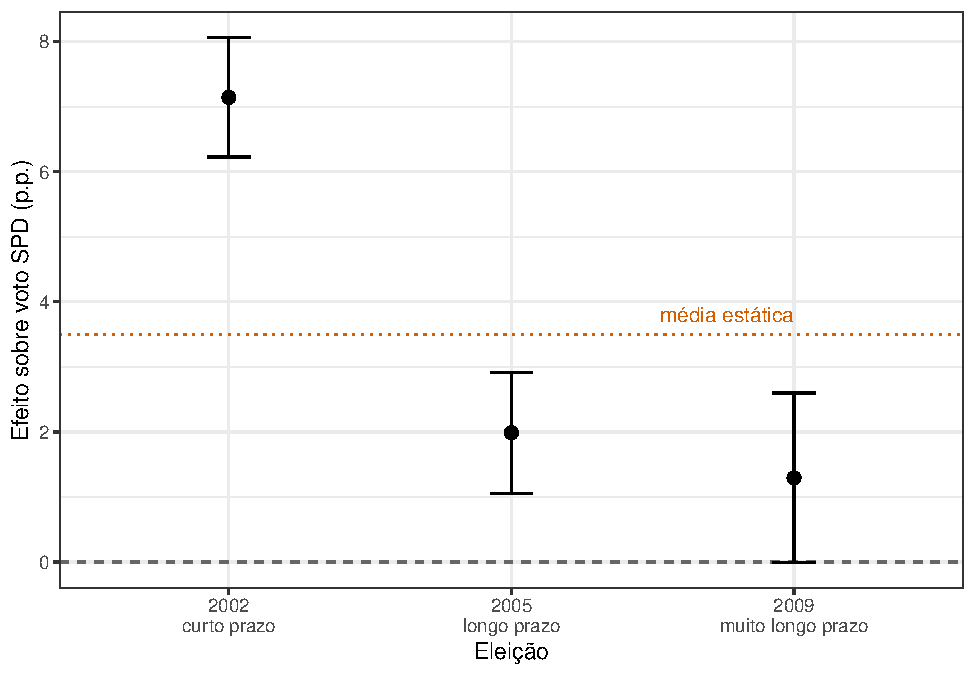
\includegraphics[keepaspectratio,alt={\label{fig:elbe-dynamic-plot}Efeitos da enchente do Elbe sobre o voto no SPD por horizonte temporal. Pontos s\textless U+00E3\textgreater o coeficientes DiD; barras s\textless U+00E3\textgreater o intervalos de confian\textless U+00E7\textgreater a de 95\%.}]{bookdownproj_files/figure-latex/elbe-dynamic-plot-1.pdf}}
\caption{\label{fig:elbe-dynamic-plot}Efeitos da enchente do Elbe sobre o voto no SPD por horizonte temporal. Pontos s\textless U+00E3\textgreater o coeficientes DiD; barras s\textless U+00E3\textgreater o intervalos de confian\textless U+00E7\textgreater a de 95\%.}
\end{figure}

O ponto didático é que o coeficiente estático não é ``o efeito em 2005''; ele é uma média que mistura os horizontes. Para interpretar persistência, devemos comparar o efeito de 2005 com o efeito de 2002. A estimativa de 2005 é positiva, mas muito menor que a de 2002, o que sustenta a conclusão de que parte do ganho de curto prazo persistiu, mas decaiu substancialmente.

\subsection{Extensões e escolhas de desenho}\label{extensuxf5es-e-escolhas-de-desenho}

\subsubsection{Diferenças triplas}\label{diferenuxe7as-triplas}

Uma extensão natural do DiD é o modelo de \textbf{diferenças triplas} (DDD). A ideia é usar uma terceira dimensão de comparação para descontar uma falha de tendências paralelas que seria comum aos grupos expostos e não expostos. Por exemplo, suponha que uma política estadual afete apenas mulheres, e queremos comparar estados tratados e não tratados antes e depois da política. Um DiD simples compara mulheres em estados tratados versus mulheres em estados de controle. Um DDD acrescenta homens como um terceiro grupo, assumindo que qualquer choque diferencial entre estados tratados e controles afetaria homens e mulheres de forma similar.

Com dois períodos, uma especificação típica é:

\[
Y_{igst} = \alpha_{ig} + \lambda_{gt} + \eta_{st} + \tau (Treat_s \times Post_t \times Grupo_g) + \varepsilon_{igst}
\]

onde \(s\) indexa estados, \(t\) tempo e \(g\) grupos. O coeficiente \(\tau\) compara a mudança do grupo exposto nos estados tratados com: (i) a mudança do grupo exposto nos estados de controle, (ii) a mudança do grupo não exposto nos estados tratados e (iii) a mudança do grupo não exposto nos estados de controle. A suposição não é que todas as tendências sejam paralelas; é que a \textbf{falha} de tendências paralelas entre estados seria a mesma no grupo exposto e no grupo não exposto.

DDD é útil quando há um grupo substantivamente próximo que não deveria ser afetado pela política, mas não é uma solução automática. Se o grupo ``não exposto'' também reage à política, ou se a diferença de tendências entre expostos e não expostos muda justamente nos locais tratados, o estimador perde interpretação causal.

\subsubsection{Tratamento contínuo, múltiplo ou reversível}\label{tratamento-contuxednuo-muxfaltiplo-ou-reversuxedvel}

A maior parte deste capítulo assume tratamento binário e absorvente: uma unidade passa de não tratada para tratada e permanece tratada. Muitas aplicações não têm essa estrutura. A intensidade de fiscalização, o valor de uma transferência, a alíquota de imposto ou a exposição a um programa podem variar continuamente. Nesse caso, a pergunta ``qual é o efeito do tratamento?'' precisa ser substituída por perguntas mais precisas:

\begin{itemize}
\tightlist
\item
  Qual é o efeito de receber dose \(d\) em vez de dose zero entre unidades que receberam dose \(d\)?
\item
  Qual é o efeito marginal de aumentar a dose em torno de \(d\)?
\item
  Há uma categoria de dose zero que possa servir como baseline?
\item
  O tratamento é reversível, acumulativo ou depende da história de exposição?
\end{itemize}

Callaway, Goodman-Bacon, and Sant'Anna (\citeproc{ref-callawaygoodmanbaconsantanna2024}{2024}) mostram que DiD com tratamento contínuo requer muito mais cuidado com o estimando. O TWFE pode estimar uma média ponderada de efeitos marginais ou de contrastes entre doses, mas essa média pode não corresponder ao parâmetro substantivo de interesse. A recomendação prática é começar por discretizar a pergunta causal: ``comparar quais doses com quais doses?'' Quando houver grupos de dose bem definidos, uma regressão em primeiras diferenças com indicadores de dose pode ser mais transparente do que um único coeficiente linear.

Problemas parecidos aparecem com \textbf{múltiplos tratamentos}. Se unidades podem receber combinações de políticas, ou mover-se entre categorias de tratamento, os coeficientes de TWFE podem misturar efeitos próprios, efeitos cruzados e pesos difíceis de interpretar (\citeproc{ref-hull2018}{Hull 2018}; \citeproc{ref-goldsmith-pinkham2024}{Goldsmith-Pinkham, Hull, and Kolesár 2024}). Nesses casos, defina primeiro o contraste causal desejado e só depois escolha o estimador.

\subsubsection{Adoção aleatória no tempo}\label{adouxe7uxe3o-aleatuxf3ria-no-tempo}

Até aqui, justificamos DiD como uma hipótese sobre o modelo de \(Y(0)\): na ausência de tratamento, as trajetórias teriam sido paralelas. Outra forma de pensar o desenho é perguntar se o \textbf{momento de adoção} pode ser tratado como quase aleatório, possivelmente condicional em covariáveis. Essa é a perspectiva design-based de Athey and Imbens (\citeproc{ref-atheyimbens2022}{2022}) e das discussões pedagógicas de Hull (\citeproc{ref-hull2024metrix}{2024}) e Goldsmith-Pinkham (\citeproc{ref-goldsmithpinkham2026applied}{2026}).

Em um rollout escalonado, a pergunta deixa de ser apenas ``tratados e controles teriam tendências paralelas?'' e passa a incluir: ``por que algumas unidades adotaram em 2017, outras em 2019 e outras nunca adotaram?'' Se o timing foi definido por fila administrativa, sorteio, limiar institucional ou restrição operacional plausivelmente exógena, podemos explorar esse mecanismo de atribuição. Se o timing foi escolhido estrategicamente por unidades que antecipavam ganhos, a identificação volta a depender fortemente de modelar o contrafactual.

Na prática, vale sempre descrever o processo político-administrativo de adoção. Em DiD, narrativa institucional não é ornamento: ela define quais comparações são críveis.

\subsubsection{DiD versus variável dependente defasada}\label{did-versus-variuxe1vel-dependente-defasada}

Uma pergunta comum é por que não estimar simplesmente:

\[
Y_{it} = \alpha + \tau D_{it} + \rho Y_{i,t-1} + \varepsilon_{it}
\]

Esse modelo com variável dependente defasada (LDV) não é uma versão ``mais controlada'' do DiD. Ele impõe uma lógica diferente: seleção em observáveis condicionada ao resultado passado. O DiD, por outro lado, permite que tratados e controles tenham níveis diferentes antes da política, desde que suas tendências contrafactuais sejam paralelas. Controlar por \(Y_{i,t-1}\) pode ser apropriado em alguns desenhos, mas muda o estimando e a suposição de identificação. Em painéis curtos com efeitos fixos, ainda há problemas adicionais de painel dinâmico, como o viés de Nickell (\citeproc{ref-nickell1981}{Nickell 1981}).

Uma forma prática de apresentar a diferença é estimar ambos como análise de sensibilidade, mas não tratá-los como substitutos mecânicos. Se DiD e LDV dão respostas muito diferentes, isso é evidência de que o desenho depende de suposições fortes sobre a evolução de \(Y(0)\).

\subsubsection{Checklist para aplicar DiD}\label{checklist-para-aplicar-did}

Antes de estimar, responda explicitamente:

\begin{enumerate}
\def\labelenumi{\arabic{enumi}.}
\tightlist
\item
  \textbf{Tratamento:} é binário, contínuo ou múltiplo? É absorvente ou reversível? Há antecipação provável?
\item
  \textbf{Timing:} há uma única data de adoção, adoção escalonada ou todos são eventualmente tratados?
\item
  \textbf{Contrafactual:} quem é o grupo de comparação para cada coorte e período? Existem unidades nunca tratadas ou apenas ainda-não-tratadas?
\item
  \textbf{Estimando:} o interesse é ATT médio, efeito por coorte, efeito por horizonte, efeito de curto prazo, longo prazo ou dose-resposta?
\item
  \textbf{Identificação:} a hipótese é PT incondicional, PT condicional, adoção quase aleatória no tempo, ou um modelo mais forte de contrafactual?
\item
  \textbf{Escala:} PT é mais plausível em níveis, logs, taxas ou outra transformação?
\item
  \textbf{Inferência:} qual é o nível de atribuição do tratamento? Quantos clusters independentes existem? Há poucos tratados?
\item
  \textbf{Diagnósticos:} que pré-tendências, placebos, bandas simultâneas ou análises HonestDiD são viáveis?
\item
  \textbf{Robustez:} o resultado sobrevive a estimadores modernos, mudanças razoáveis de amostra, escala e definição de tratamento?
\item
  \textbf{Interpretação:} o coeficiente estimado responde à pergunta substantiva ou é apenas uma média conveniente?
\end{enumerate}

Esse checklist é inspirado nas aulas de Hull (\citeproc{ref-hull2024metrix}{2024}) e Goldsmith-Pinkham (\citeproc{ref-goldsmithpinkham2026applied}{2026}), que enfatizam que DiD deve começar pela definição do desenho e do estimando, não pela escolha automática de uma regressão.

\subsection{Exercícios sugeridos}\label{exercuxedcios-sugeridos}

\begin{enumerate}
\def\labelenumi{\arabic{enumi}.}
\item
  \textbf{Verdadeiro, falso ou incerto.} Avalie e justifique: ``Um DiD com uma única data de adoção sofre com pesos negativos''; ``um teste de pré-tendências valida o desenho''; ``é sempre melhor clusterizar no nível mais conservador''; ``se todos são eventualmente tratados, DiD é impossível''.
\item
  \textbf{Forma funcional.} Simule duas séries que são paralelas em níveis, transforme o outcome em log e mostre que as tendências deixam de ser paralelas. Depois simule duas séries paralelas em logs e repita o exercício em níveis.
\item
  \textbf{Contaminação de event study.} Usando dados simulados com três coortes, estime um event study TWFE tradicional e um \texttt{sunab()}. Compare os coeficientes de pré-tratamento e explique por que o teste de pré-tendências pode ser enganoso.
\item
  \textbf{Inferência.} Reestime o DiD do Obra Transparente com erros-padrão clusterizados no nível da obra e no nível do município. Explique qual é o nível correto e por quê.
\item
  \textbf{Checklist aplicado.} Escolha um paper com DiD em ciência política. Preencha o checklist acima em uma página: tratamento, timing, estimando, contrafactual, inferência, diagnósticos e ameaças principais.
\end{enumerate}

\subsection{Resumo}\label{resumo}

Neste capítulo, introduzimos o estimador de Diferença em Diferenças e o pressuposto central de tendências paralelas. Os pontos-chave são:

\begin{enumerate}
\def\labelenumi{\arabic{enumi}.}
\tightlist
\item
  \textbf{DiD 2×2} é intuitivo e pode ser estimado por TWFE sem os problemas específicos de comparações proibidas dos desenhos escalonados.
\item
  \textbf{Tendências paralelas} é o pressuposto de identificação central; não é testável diretamente, depende da escala do outcome e pode ser avaliado com event studies (com cautela) e análise de sensibilidade (HonestDiD).
\item
  \textbf{A inferência deve respeitar o nível de atribuição do tratamento}: em painéis, clusterização inadequada costuma subestimar a incerteza.
\item
  \textbf{Com tratamento escalonado e efeitos heterogêneos}, o TWFE pode ser enviesado. A decomposição de Goodman-Bacon (\citeproc{ref-goodmanbacon2021}{2021}) revela os pesos problemáticos, e Sun and Abraham (\citeproc{ref-sunabraham2021}{2021}) mostram a contaminação dos coeficientes dinâmicos.
\item
  \textbf{Estimadores modernos} --- Callaway and Sant'Anna (\citeproc{ref-callawaysantanna2021}{2021}), Sun and Abraham (\citeproc{ref-sunabraham2021}{2021}), Gardner (\citeproc{ref-gardner2022}{2022}) (\texttt{did2s}), Borusyak, Jaravel, and Spiess (\citeproc{ref-borusyak2024}{2024}) --- corrigem o problema e convergem para estimativas consistentes.
\item
  \textbf{Em aplicações com tratamento simultâneo} (como Obra Transparente e a enchente do Elbe), o TWFE não sofre do problema específico de comparações proibidas, mas o estimando ainda precisa acompanhar a pergunta substantiva.
\item
  \textbf{Covariáveis devem ser incluídas com cuidado}: enriquecer o modelo de \(Y(0)\) com estimação nos não-tratados ou usar PTA condicional com estimação duplamente robusta --- nunca adicionando covariáveis variantes no tempo ao TWFE ingenuamente.
\item
  \textbf{Tratamentos contínuos, múltiplos, reversíveis ou com timing quase aleatório} exigem redefinir o estimando antes de escolher o estimador.
\end{enumerate}

No próximo capítulo, discutiremos dados de painel (TSCS) de forma mais geral, incluindo as suposições de exogeneidade estrita e sequencial --- das quais as tendências paralelas são um caso especial. No capítulo 11, veremos o controle sintético como alternativa quando PT é duvidosa ou quando há poucas unidades tratadas.

\section{Time-Series Cross-Section (TSCS)}\label{time-series-cross-section-tscs}

\subsection{Introdução}\label{introduuxe7uxe3o-6}

No capítulo sobre Diferença em Diferenças, chegamos a uma ideia forte: quando o tratamento é binário e absorvente, não há antecipação e tendências paralelas são plausíveis, PT implica uma estrutura aditiva para os resultados potenciais sem tratamento. Nessa estrutura, o TWFE é a forma regressiva do DiD. Os efeitos fixos de unidade removem diferenças permanentes entre unidades; os efeitos fixos de tempo removem choques comuns; e o coeficiente do tratamento resume a comparação residual entre unidades tratadas e não tratadas ao longo do tempo.

Este capítulo começa exatamente daí. A questão agora não é repetir que TWFE pode ser lido como DiD generalizado nesse caso. A questão é entender o que acontece quando saímos desse caso limpo. O que muda quando usamos apenas um efeito fixo? O que muda quando empilhamos município, ano e estado-ano? O que sobra para identificar o coeficiente quando os efeitos fixos absorvem grande parte da variação do tratamento? E como interpretar uma regressão com efeitos fixos quando o tratamento é uma intensidade que sobe e desce, e não uma chave que liga uma vez e permanece ligada?

A motivação é prática. Em dados de painel, quase sempre queremos usar a repetição no tempo para descontar diferenças persistentes entre unidades. Municípios ricos e pobres, países democráticos e autoritários, estados com burocracias diferentes não começam do mesmo lugar. Efeitos fixos ajudam a lidar com essas diferenças de nível. Mas eles não dizem, por si só, se a variação restante do tratamento é uma boa comparação causal. Se uma política chega depois de uma piora fiscal, se a dose muda porque o outcome piorou, ou se cada estado tem sua própria tendência, o problema deixou de ser apenas ``colocar efeitos fixos''. Passa a ser dizer qual comparação sobrou e qual pressuposto torna essa comparação crível.

\textbf{Quadro-guia.} A lógica do capítulo é a seguinte:

\begin{longtable}[]{@{}
  >{\raggedright\arraybackslash}p{(\linewidth - 4\tabcolsep) * \real{0.3333}}
  >{\raggedright\arraybackslash}p{(\linewidth - 4\tabcolsep) * \real{0.3333}}
  >{\raggedright\arraybackslash}p{(\linewidth - 4\tabcolsep) * \real{0.3333}}@{}}
\toprule\noalign{}
\begin{minipage}[b]{\linewidth}\raggedright
Situação
\end{minipage} & \begin{minipage}[b]{\linewidth}\raggedright
O que a regressão faz
\end{minipage} & \begin{minipage}[b]{\linewidth}\raggedright
Pergunta que fica
\end{minipage} \\
\midrule\noalign{}
\endhead
\bottomrule\noalign{}
\endlastfoot
TWFE no DiD com tratamento absorvente & Implementa a comparação DiD sob PT e sem antecipação & O desenho empírico realmente corresponde a esse caso? \\
Um efeito fixo & Remove diferenças permanentes em uma dimensão & A variação \emph{within} ou \emph{between} remanescente é a comparação certa? \\
Dois ou mais efeitos fixos & Absorve várias dimensões de comparação & Que variação do tratamento ainda resta para estimar o coeficiente? \\
Tratamento contínuo ou variável no tempo & Usa mudanças de dose, intensidade ou exposição & Que estimando a inclinação linear está resumindo? \\
Pressuposto causal & Dá interpretação causal à variação residual & Estamos usando PT, randomização no baseline, exogeneidade estrita ou ignorabilidade sequencial? \\
\end{longtable}

Antes de discutir os modelos, vale fixar a linguagem. Dados de painel são definidos como observações repetidas de uma mesma unidade \(i = 1, \ldots, N\) no período \(t = 1, \ldots, T\). O termo tem origem em surveys em ondas, em que o mesmo indivíduo era rastreado ao longo do tempo. Em ciência política também chamamos esse tipo de dado de \textbf{Time-Series Cross-Section}, ou TSCS. A distinção foi introduzida porque surveys em ondas tipicamente possuem \(T\) pequeno, enquanto dados TSCS comuns em política comparada, Relações Internacionais e políticas públicas costumam ter \(T\) maior: países da OCDE ao longo de cinquenta anos, estados brasileiros ao longo de trinta anos, municípios ao longo de várias eleições.

Uma observação de uma variável dependente e uma variável independente é dada pelo par \((y_{it}, x_{it})\), em que \(i\) indexa a unidade e \(t\) indexa o tempo.

Tradicionalmente a literatura categorizava os dados de painel em balanceados, quando todas as unidades são observadas nos mesmos períodos, e não balanceados, quando algumas unidades têm períodos ausentes. Essa terminologia pode confundir com a ideia de balanceamento em matching. Uma alternativa mais clara é falar em painéis completos e incompletos.

Em TSCS, incompletude nem sempre significa dado ausente. Países deixam de existir, como a URSS e a Iugoslávia, e outros são criados, como Sérvia e Montenegro. O mesmo vale para estados e municípios. Não é óbvio que devemos tratar esse problema como ausência de informação. A entidade pode simplesmente não existir em parte da série. Em meu doutorado, por exemplo, estudei o efeito de regimes políticos sobre a adesão a tratados de patentes. Não é claro se a adesão da URSS em um período \(t^{\star}\) deve ser atribuída à Rússia em períodos \(t > t^{\star}\). E no caso da Iugoslávia? Essas decisões são substantivas e metodológicas.

Os dados podem ser organizados em dois formatos: \textbf{long} e \textbf{wide}. O formato long, que é o padrão em análise de dados, organiza a base com uma linha por unidade-período. O formato wide coloca cada unidade em uma única linha e distribui os períodos em colunas.

\begin{figure}
\centering
\pandocbounded{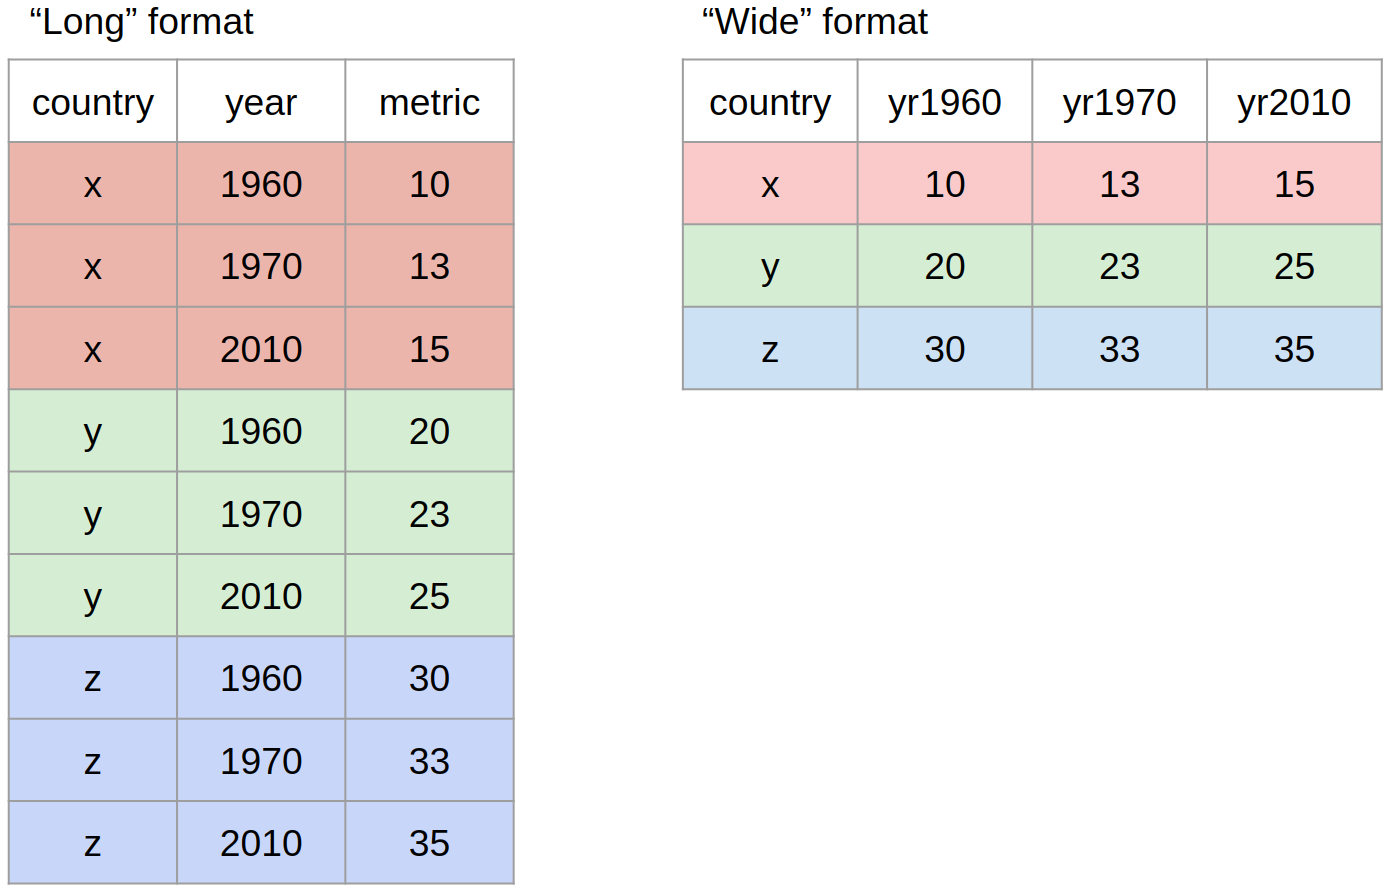
\includegraphics[keepaspectratio,alt={long vs wide format. Fonte: https://tavareshugo.github.io/r-intro-tidyverse-gapminder/09-reshaping/index.html}]{imagens/long-wide-data-shapes.png}}
\caption{long vs wide format. Fonte: \url{https://tavareshugo.github.io/r-intro-tidyverse-gapminder/09-reshaping/index.html}}
\end{figure}

\subsection{Variação within e between}\label{variauxe7uxe3o-within-e-between}

Uma distinção importante em dados de painel é entre variação \emph{within} e variação \emph{between}. A variação \emph{between} compara unidades diferentes. A variação \emph{within} compara a mesma unidade consigo mesma ao longo do tempo.

Imagine que temos uma variável \(x_{it}\) medida para \(N\) indivíduos em \(T\) períodos. Podemos calcular três médias:

\begin{enumerate}
\def\labelenumi{\arabic{enumi}.}
\item
  Média individual:
  \[
  \bar{x}_i = \frac{1}{T}\sum_{t=1}^T x_{it}.
  \]
\item
  Média temporal:
  \[
  \bar{x}_t = \frac{1}{N}\sum_{i=1}^N x_{it}.
  \]
\item
  Média geral:
  \[
  \bar{x} = \frac{1}{NT}\sum_{i=1}^N\sum_{t=1}^T x_{it}.
  \]
\end{enumerate}

A variação \emph{between} mede quanto as médias das unidades diferem da média geral:
\[
B = \sum_{i=1}^N T_i(\bar{x}_i - \bar{x})^2.
\]
Se o painel é completo, \(T_i = T\) para todas as unidades.

A variação \emph{within} mede quanto cada observação se afasta da média da própria unidade:
\[
W = \sum_{i=1}^N \sum_{t=1}^{T_i}(x_{it} - \bar{x}_i)^2.
\]

A variação total em torno da média geral pode ser decomposta em:
\[
\sum_{i=1}^N\sum_{t=1}^{T_i} (x_{it} - \bar{x})^2 = W + B.
\]

Essa decomposição é útil porque efeitos fixos decidem qual parte da variação será usada pelo estimador. Se removemos as diferenças fixas entre unidades, o coeficiente será estimado com variação dentro das unidades. Se removemos choques comuns a cada período, o coeficiente será estimado com comparações dentro do mesmo período. Com muitos efeitos fixos, a variação que resta pode ser pequena e substantivamente estreita.

\subsection{Efeitos fixos como residualização}\label{efeitos-fixos-como-residualizauxe7uxe3o}

A forma mais simples de entender efeitos fixos é pensar em residualização. Um efeito fixo remove a média de uma dimensão da base. Depois disso, a regressão usa apenas o que sobrou.

\begin{figure}
\centering
\pandocbounded{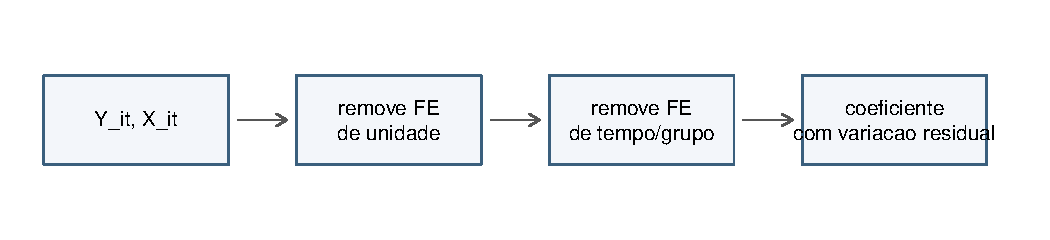
\includegraphics[keepaspectratio,alt={\label{fig:fe-residualizacao-diagrama}Efeitos fixos como residualização. A regressão final usa apenas a variação que permanece depois de remover as dimensões absorvidas pelos efeitos fixos.}]{bookdownproj_files/figure-latex/fe-residualizacao-diagrama-1.pdf}}
\caption{\label{fig:fe-residualizacao-diagrama}Efeitos fixos como residualização. A regressão final usa apenas a variação que permanece depois de remover as dimensões absorvidas pelos efeitos fixos.}
\end{figure}

Considere o modelo:
\[
y_{it} = \alpha_i + \beta x_{it} + u_{it}.
\]

O efeito fixo de unidade, \(\alpha_i\), captura tudo que é fixo na unidade ao longo do tempo: geografia, história institucional, cultura política persistente, características de origem, ou qualquer outro atributo que não muda no período analisado. Se subtraímos a média da unidade de cada variável, obtemos:
\[
y_{it} - \bar{y}_i = \beta (x_{it} - \bar{x}_i) + (u_{it} - \bar{u}_i).
\]

Definindo \(\tilde{y}_{it} = y_{it} - \bar{y}_i\) e \(\tilde{x}_{it} = x_{it} - \bar{x}_i\), temos:
\[
\tilde{y}_{it} = \beta \tilde{x}_{it} + \tilde{u}_{it}.
\]

Essa é a intuição do estimador de efeitos fixos: ele compara cada unidade consigo mesma. Toda variável que não muda dentro da unidade desaparece da equação. Isso é uma vantagem quando a fonte de confusão é invariante no tempo. Também é um custo, pois qualquer variável de interesse sem variação dentro da unidade não pode ser estimada.

\subsubsection{Um efeito fixo}\label{um-efeito-fixo}

Com apenas efeito fixo de unidade:
\[
y_{it} = \alpha_i + \beta x_{it} + u_{it},
\]
o coeficiente \(\beta\) é identificado pela variação de \(x_{it}\) dentro da unidade ao longo do tempo. Esse modelo controla características fixas da unidade, mas não controla choques comuns a todos em determinado período.

Com apenas efeito fixo de tempo:
\[
y_{it} = \lambda_t + \beta x_{it} + u_{it},
\]
o coeficiente \(\beta\) é identificado por diferenças entre unidades dentro do mesmo período. Esse modelo controla choques comuns de tempo, mas não controla diferenças fixas entre unidades.

Os dois modelos respondem a perguntas diferentes. O primeiro pergunta se uma unidade tem valores maiores de \(y\) nos períodos em que seu próprio \(x\) está maior. O segundo pergunta se, em um mesmo período, unidades com maior \(x\) têm maior \(y\).

\subsubsection{Dois efeitos fixos}\label{dois-efeitos-fixos}

Com efeitos fixos de unidade e tempo:
\[
y_{it} = \alpha_i + \lambda_t + \beta x_{it} + u_{it},
\]
o coeficiente é estimado com a variação de \(x_{it}\) que permanece depois de remover diferenças médias entre unidades e diferenças médias entre períodos.

Esse é o caso que vimos no capítulo de DiD. Quando \(x_{it}\) é um indicador binário de tratamento, o TWFE pode ser interpretado como uma generalização do DiD sob pressupostos apropriados. A interpretação com uma variável contínua é diferente. O coeficiente não compara simplesmente tratados e controles. Ele mede uma inclinação: quanto \(y\) muda, em média, quando a parte residual de \(x\) aumenta uma unidade.

\subsubsection{Mais de dois efeitos fixos}\label{mais-de-dois-efeitos-fixos}

Em aplicações reais, usamos frequentemente mais de dois efeitos fixos. Isso muda a comparação efetiva.

Considere um painel de municípios ao longo do tempo:
\[
y_{imt} = \alpha_m + \lambda_t + \beta x_{imt} + u_{imt},
\]
em que \(m\) indexa municípios. O efeito fixo de município remove diferenças permanentes entre municípios. O efeito fixo de tempo remove choques comuns a todos os municípios em cada período.

Agora suponha que adicionamos efeitos fixos de estado-ano:
\[
y_{imt} = \alpha_m + \delta_{st} + \beta x_{imt} + u_{imt},
\]
em que \(\delta_{st}\) é um efeito fixo para cada combinação entre estado \(s\) e período \(t\). O coeficiente passa a ser identificado por variação entre municípios dentro do mesmo estado e no mesmo período, depois de controlar diferenças fixas entre municípios. Choques específicos de São Paulo em 2018, Bahia em 2018, São Paulo em 2019, e assim por diante, são absorvidos.

Isso pode ser desejável quando há choques estaduais que afetariam simultaneamente o tratamento e o outcome. Mas também pode remover a própria variação do tratamento. Se \(x_{imt}\) varia apenas no nível estado-ano, então \(\delta_{st}\) absorve completamente \(x_{imt}\) e o coeficiente não pode ser estimado.

Também é comum encontrar efeitos fixos redundantes. Se cada município pertence a apenas um estado, então efeitos fixos de município já absorvem diferenças fixas entre estados. Nesse caso, adicionar efeitos fixos de estado não acrescenta controle substantivo; eles são colineares com os efeitos fixos de município.

Uma regra prática é perguntar: depois de todos os efeitos fixos, quem está sendo comparado com quem? Se a resposta não é clara, a interpretação do coeficiente também não é clara.

Considere agora uma mini-base com três municípios observados em três anos. Os municípios A e B pertencem ao mesmo estado; C pertence a outro. A coluna \texttt{x} é propositalmente contínua: pense em uma dose de tratamento, como gasto per capita, intensidade de fiscalização ou cobertura de um programa. Se \texttt{x} fosse binária, a lógica da residualização seria a mesma; o ponto importante é que a variável que entra na regressão depois dos efeitos fixos não é o \texttt{x} original, mas o resíduo de \texttt{x}.

Com um efeito fixo de município, a conta é:
\[
\tilde{x}_{it}^{(m)} = x_{it} - \bar{x}_i.
\]
Com efeitos fixos de município e ano, em um painel completo e balanceado, a conta é:
\[
\tilde{x}_{it}^{(m,t)} = x_{it} - \bar{x}_i - \bar{x}_t + \bar{x}.
\]
Com efeitos fixos de município e estado-ano, a conta é o resíduo de uma regressão auxiliar de \(x_{imt}\) nos próprios efeitos fixos:
\[
\tilde{x}_{imt}^{(m,st)} =
\operatorname{resid}\left(x_{imt} \sim \alpha_m + \delta_{st}\right).
\]
Essa última fórmula é menos transparente porque, com efeitos fixos sobrepostos ou aninhados, o que sobra é definido pela projeção linear de \texttt{x} no espaço não explicado pelas dummies.

Uma linha concreta ajuda. Para o município A em 2020, \(x = 2\), a média de A é \(3{,}33\), a média de 2020 é \(4{,}33\) e a média geral é \(5{,}22\). Portanto, após FE de município, temos \(2 - 3{,}33 = -1{,}33\). Após FE de município e ano, temos \(2 - 3{,}33 - 4{,}33 + 5{,}22 = -0{,}44\). A tabela repete essa mesma lógica para todas as linhas.

\begin{table}

\caption{\label{tab:toy-panel-residualization}Mini-base com tratamento contínuo e valores de x após residualização por diferentes conjuntos de efeitos fixos.}
\centering
\begin{tabular}[t]{l|l|r|r|r|r|r}
\hline
Município & Estado & Ano & x & x após FE município & x após FE município + ano & x após FE município + estado-ano\\
\hline
A & SP & 2020 & 2 & -1.33 & -0.44 & -0.33\\
\hline
A & SP & 2021 & 3 & -0.33 & -0.11 & 0.17\\
\hline
A & SP & 2022 & 5 & 1.67 & 0.56 & 0.17\\
\hline
B & SP & 2020 & 4 & -0.67 & 0.22 & 0.33\\
\hline
B & SP & 2021 & 4 & -0.67 & -0.44 & -0.17\\
\hline
B & SP & 2022 & 6 & 1.33 & 0.22 & -0.17\\
\hline
C & BA & 2020 & 7 & -0.67 & 0.22 & 0.00\\
\hline
C & BA & 2021 & 8 & 0.33 & 0.56 & 0.00\\
\hline
C & BA & 2022 & 8 & 0.33 & -0.78 & 0.00\\
\hline
\end{tabular}
\end{table}

Note a lógica: efeitos fixos de município removem diferenças persistentes entre A, B e C; efeitos fixos de ano removem choques comuns a todos; efeitos fixos de estado-ano deixam apenas comparações dentro do mesmo estado e ano. Como C é o único município de seu estado nesta mini-base, a especificação com município e estado-ano deixa pouca informação útil para C. Esse é exatamente o tipo de perda de variação que pode ocorrer em aplicações reais.

\textbf{Pausa.} Antes de interpretar qualquer coeficiente com efeitos fixos, faça três perguntas:

\begin{enumerate}
\def\labelenumi{\arabic{enumi}.}
\tightlist
\item
  Quem está sendo comparado com quem?
\item
  Qual variação do tratamento sobrou depois dos efeitos fixos?
\item
  Qual hipótese torna essa variação residual plausivelmente causal?
\end{enumerate}

\subsubsection{Tratamento contínuo}\label{tratamento-contuxednuo}

Quando o tratamento é contínuo, a interpretação do TWFE precisa ser formulada em termos de dose ou intensidade. O modelo:
\[
y_{it} = \alpha_i + \lambda_t + \beta d_{it} + u_{it}
\]
estima a associação entre a parte residual da dose \(d_{it}\) e a parte residual de \(y_{it}\).

Se \(d_{it}\) mede o valor de uma transferência federal por habitante, por exemplo, \(\beta\) indica a mudança esperada em \(y\) associada a uma unidade adicional dessa transferência, depois de remover médias de unidade e de tempo. Essa interpretação depende de três condições.

Primeiro, deve haver suporte. Precisamos observar unidades comparáveis com diferentes níveis residuais de dose. Segundo, a forma funcional linear precisa ser razoável no intervalo de doses observado. Terceiro, a variação residual da dose precisa ser plausivelmente exógena, dado o conjunto de efeitos fixos e controles.

Com tratamento binário, a pergunta típica é sobre a diferença entre estar tratado e não estar tratado. Com tratamento contínuo, a pergunta passa a ser sobre a curva dose-resposta. Se o efeito de sair de 0 para 1 é diferente do efeito de sair de 10 para 11, um único coeficiente linear pode esconder heterogeneidade substantiva.

\subsection{OVB e efeitos fixos}\label{ovb-e-efeitos-fixos}

O principal atrativo dos efeitos fixos é lidar com viés de variável omitida causado por características não observadas e invariantes no tempo.

Suponha o DAG abaixo, em que \(a\) é uma variável invariante no tempo e não observada:

\begin{Shaded}
\begin{Highlighting}[]
\FunctionTok{library}\NormalTok{(ggdag)}
\NormalTok{dag }\OtherTok{\textless{}{-}} \FunctionTok{dagify}\NormalTok{(}
\NormalTok{  y }\SpecialCharTok{\textasciitilde{}}\NormalTok{ x }\SpecialCharTok{+}\NormalTok{ a,}
\NormalTok{  x }\SpecialCharTok{\textasciitilde{}}\NormalTok{ a,}
  \AttributeTok{latent =} \StringTok{"a"}
\NormalTok{)}

\FunctionTok{ggdag}\NormalTok{(dag)}
\end{Highlighting}
\end{Shaded}

\begin{figure}
\centering
\pandocbounded{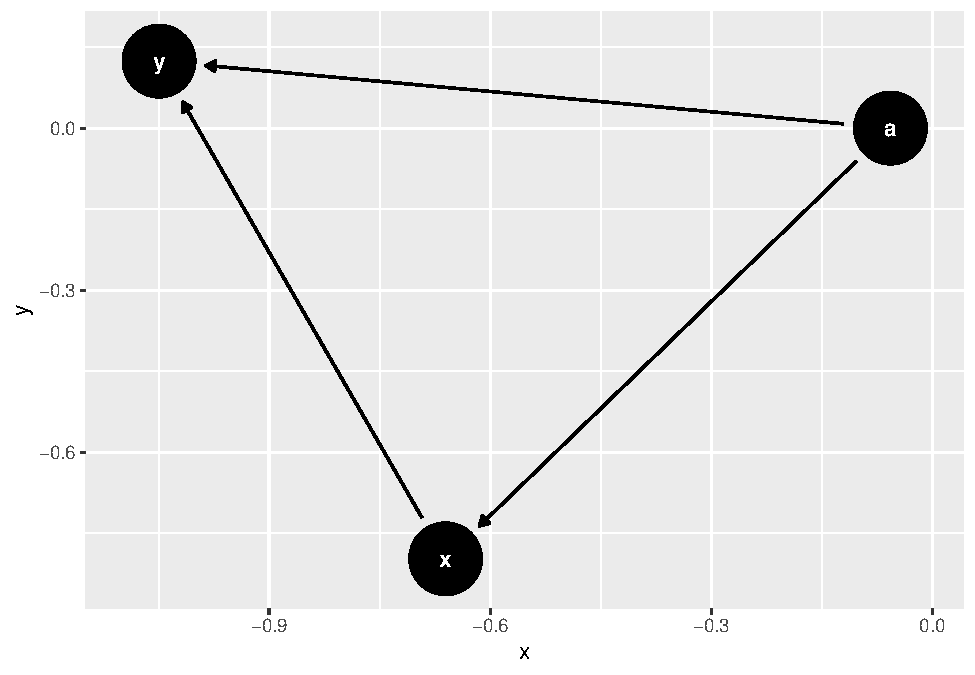
\includegraphics[keepaspectratio,alt={\label{fig:dag-fe}DAG de OVB com confundidor fixo não observado. O painel ajuda quando a fonte de confusão, aqui representada por a\_i, é constante dentro da unidade ao longo do tempo.}]{bookdownproj_files/figure-latex/dag-fe-1.pdf}}
\caption{\label{fig:dag-fe}DAG de OVB com confundidor fixo não observado. O painel ajuda quando a fonte de confusão, aqui representada por \(a_i\), é constante dentro da unidade ao longo do tempo.}
\end{figure}

Essa estrutura leva ao problema clássico de variável omitida. Dados de painel nos permitem remover essa variável de confusão quando ela é fixa na unidade. Suponha a forma paramétrica:
\[
y_{it} = \alpha + \beta_0 x_{it} + a_i + e_{it}.
\]

\textbf{Box técnico (para leitura ou backup).} A derivação abaixo mostra, passo a passo, como a centralização por unidade remove \(a_i\). Em uma aula oral curta, a mensagem principal é apenas que subtrair a média da unidade elimina tudo que é constante dentro dela.

Para simplificar, suponha que o painel é completo. A média da unidade é:
\[
\begin{aligned}
\bar{y}_i &= \frac{1}{T}\sum_{t=1}^T y_{it} \\
         &= \frac{1}{T}\sum_{t=1}^T (\alpha + \beta_0 x_{it} + a_i + e_{it}) \\
         &= \alpha + \beta_0 \bar{x}_i + a_i + \bar{e}_i.
\end{aligned}
\]

Subtraindo essa média da equação original:
\[
\begin{aligned}
y_{it} - \bar{y}_i
  &= \alpha + \beta_0 x_{it} + a_i + e_{it}
     - (\alpha + \beta_0 \bar{x}_i + a_i + \bar{e}_i) \\
  &= \beta_0(x_{it} - \bar{x}_i) + (e_{it} - \bar{e}_i).
\end{aligned}
\]

O termo \(a_i\) desaparece. Isso mostra exatamente o que efeitos fixos fazem: eles removem a parte da confusão que é constante dentro da unidade.

A pergunta causal permanece. Depois de remover \(a_i\), a variação de \(x_{it} - \bar{x}_i\) pode ser tratada como exógena? A resposta depende do desenho, do tratamento e dos pressupostos de identificação.

\subsection{Efeitos aleatórios e Mundlak}\label{efeitos-aleatuxf3rios-e-mundlak}

Efeitos fixos não são a única forma de modelar heterogeneidade entre unidades. Uma alternativa é o modelo de efeitos aleatórios. Um modelo simples pode ser escrito como:
\[
y_{it} = \beta_0 + \beta_1 x_{it} + \mu_i + e_{it},
\]
em que \(\mu_i\) é um intercepto específico da unidade.

No modelo de efeitos aleatórios, assumimos tipicamente que:
\[
\mu_i \sim N(0, \sigma^2_{\mu})
\]
e
\[
e_{it} \sim N(0, \sigma^2_e).
\]

Isso também pode ser entendido como \emph{partial pooling}. Se \(\sigma^2_{\mu} = 0\), todas as unidades têm o mesmo intercepto e temos uma regressão pooled. Se \(\sigma^2_{\mu}\) é muito grande, cada unidade pode ter um intercepto muito diferente das demais, aproximando uma regressão com efeitos fixos.

A suposição substantiva forte é:
\[
\mathbb{E}[\mu_i \mid x_{i1}, x_{i2}, \ldots, x_{iT}] = 0.
\]

Em palavras, o intercepto específico da unidade não pode estar correlacionado com a trajetória do tratamento ou da variável independente. Essa suposição é frequentemente implausível em ciência política. Municípios com maior capacidade estatal, por exemplo, podem ter níveis médios maiores de gasto, maior probabilidade de receber programas e melhores outcomes.

Textos de econometria costumam apresentar essa escolha como uma decisão entre efeitos fixos e efeitos aleatórios usando o teste de Hausman. A hipótese nula do teste é que o estimador de efeitos aleatórios é consistente. Em termos substantivos, isso quer dizer que a heterogeneidade não observada da unidade, \(\mu_i\), não está correlacionada com os regressores. Sob essa hipótese, efeitos fixos e efeitos aleatórios estimam o mesmo parâmetro, mas efeitos aleatórios é mais eficiente. Se rejeitamos a nula, a diferença entre os dois estimadores é sistemática, o que sugere que efeitos aleatórios está usando variação contaminada pela correlação entre \(\mu_i\) e \(x_{it}\).

O teste de Hausman é útil como diagnóstico, mas não resolve sozinho a pergunta causal. Ele testa uma implicação estatística da especificação, não prova que efeitos fixos identificam um efeito causal. A correção de Mundlak ajuda justamente porque torna explícita a fonte do problema: em vez de assumir que \(\mu_i\) é independente da trajetória de \(x_{it}\), adicionamos ao modelo a média da unidade, \(\bar{x}_i\). Se \(\bar{x}_i\) explica \(y_{it}\), há evidência de que a variação \emph{between} carrega informação diferente da variação \emph{within}. Nesse sentido, testar os coeficientes das médias de unidade em um modelo de efeitos aleatórios correlacionados é uma forma direta de perguntar se a hipótese forte dos efeitos aleatórios é plausível.

Bell e Jones, seguindo Mundlak, mostram uma forma útil de enxergar o problema. A variável \(x_{it}\) pode ser decomposta em dois componentes:
\[
x_{it} = \bar{x}_i + (x_{it} - \bar{x}_i).
\]

O primeiro termo, \(\bar{x}_i\), captura diferenças entre unidades. O segundo, \(x_{it} - \bar{x}_i\), captura variação dentro da unidade ao longo do tempo. Um modelo de efeitos aleatórios que inclui a média da unidade separa essas duas fontes de variação:
\[
y_{it} = \beta_0 + \beta_W (x_{it} - \bar{x}_i) + \beta_B \bar{x}_i + \mu_i + e_{it}.
\]

Aqui, \(\beta_W\) é o efeito associado à variação \emph{within}, e \(\beta_B\) é o efeito associado à variação \emph{between}. Quando os dois são diferentes, um modelo que impõe um único coeficiente para \(x_{it}\) mistura processos distintos.

\subsection{Histórias de tratamento e estimandos}\label{histuxf3rias-de-tratamento-e-estimandos}

Em dados TSCS, o tratamento de hoje pode depender do tratamento de ontem, e o resultado de hoje pode depender da história inteira do tratamento. Por isso, precisamos falar de histórias.

Todos os tratamentos recebidos por uma unidade formam a história do tratamento:
\[
X_i = \{x_{i1}, x_{i2}, \ldots, x_{iT}\}.
\]

A história parcial até \(t\) é:
\[
X_{i,1:t} = \{x_{i1}, x_{i2}, \ldots, x_{it}\}.
\]

Com tratamento binário, se a ordem importa, cada sequência é substantivamente distinta. Um país que foi democracia nos cinco primeiros períodos e ditadura nos cinco últimos pode não ser comparável a um país que viveu a sequência inversa, mesmo que ambos tenham o mesmo número total de períodos democráticos.

De maneira geral, podemos escrever:
\[
Y_{it}(x_{i1}, x_{i2}, \ldots, x_{it}).
\]

Se a ordem não importa e apenas a dose acumulada importa, podemos escrever uma restrição mais forte:
\[
Y_{it}(x_{i1}, x_{i2}, \ldots, x_{it}) =
Y_{it}\left(\sum_{s=1}^t x_{is}\right).
\]

Há muitos estimandos possíveis. Podemos estar interessados no efeito de uma história completa de tratamento:
\[
\tau_{X,X'} =
\mathbb{E}[Y_{it}(X_{i,1:t}) - Y_{it}(X'_{i,1:t})].
\]

Podemos estar interessados no efeito de uma história recente:
\[
\mathbb{E}[Y_{it}(X_{i,t-j:t}) - Y_{it}(X'_{i,t-j:t})].
\]

Ou podemos estar interessados em um efeito contemporâneo, mantendo a história passada como dada e alterando apenas o tratamento no período atual:
\[
\tau_c(t) =
\mathbb{E}[Y_{it}(X_{i,1:t-1}, 1) - Y_{it}(X_{i,1:t-1}, 0)].
\]

Essas quantidades são diferentes. O erro comum é estimar um coeficiente em painel e falar em ``o efeito do tratamento'' sem dizer qual contraste causal está sendo estimado.

\subsection{Quatro pressupostos de identificação}\label{quatro-pressupostos-de-identificauxe7uxe3o}

Agora podemos separar quatro pressupostos que aparecem com frequência em dados de painel: tendências paralelas, randomização no baseline, exogeneidade estrita e ignorabilidade sequencial. Eles não são a mesma coisa.

A confusão mais comum é tratar tendências paralelas como se fosse apenas outro nome para ignorabilidade. Essa tradução é imprecisa. Ignorabilidade fala sobre atribuição do tratamento. Tendências paralelas fala sobre a evolução do resultado contrafactual sem tratamento.

\subsubsection{Mapa dos pressupostos}\label{mapa-dos-pressupostos}

\begin{table}

\caption{\label{tab:pressupostos-matriz}Mapa dos quatro pressupostos. As cores distinguem famílias de suposições: tendências, atribuição inicial, exogeneidade de regressão e atribuição sequencial.}
\centering
\begin{tabular}[t]{l|l|l|l}
\hline
Pressuposto & Experimento imaginário & O que permite & O que exclui\\
\hline
Tendências paralelas & Tratados e controles teriam evoluído da mesma forma sem tratamento & DiD/TWFE como comparação de mudanças contrafactuais & Seleção em tendências não tratadas\\
\hline
Randomização no baseline & A sequência inteira de tratamento é sorteada antes do painel começar & Comparar histórias de tratamento como grupos experimentais & Seleção dinâmica baseada em resultados passados\\
\hline
Exogeneidade estrita & O tratamento não responde a choques passados, presentes ou futuros do outcome & Interpretar FE/TWFE sob modelo linear & Feedback de choques de y para valores futuros de x\\
\hline
Ignorabilidade sequencial & Em cada período, o tratamento é atribuído condicionalmente à história observada & Estimar regimes dinâmicos sob seleção em observáveis & Confusão não observada variante no tempo\\
\hline
\end{tabular}
\end{table}

\textbf{Pausa.} Ao escolher uma dessas hipóteses, pergunte: estou fazendo uma afirmação sobre a trajetória contrafactual do outcome, ou sobre o mecanismo de atribuição do tratamento?

\subsubsection{Detalhamento dos pressupostos}\label{detalhamento-dos-pressupostos}

\subsubsection{Tendências paralelas}\label{tenduxeancias-paralelas-1}

Tendências paralelas é o pressuposto que sustenta o DiD. Em sua forma básica, com dois períodos, o estimando usual para os tratados é:
\[
ATT = \mathbb{E}[Y_{i1}(1)-Y_{i1}(0)\mid D_i=1].
\]

Observamos \(Y_{i1}(1)\) para os tratados, mas não observamos \(Y_{i1}(0)\). A hipótese de tendências paralelas diz:
\[
\mathbb{E}[Y_{i1}(0)-Y_{i0}(0)\mid D_i=1]
=
\mathbb{E}[Y_{i1}(0)-Y_{i0}(0)\mid D_i=0].
\]

Como antes do tratamento vale \(Y_{i0}=Y_{i0}(0)\), usamos a evolução dos controles para imputar o contrafactual dos tratados.

Repare o que essa hipótese não diz. PT não exige:
\[
D_i \perp Y_{i1}(0).
\]

Tratados e controles podem ser diferentes em níveis. O que PT exige é uma igualdade sobre a mudança média do resultado não tratado:
\[
\Delta Y_i(0)=Y_{i1}(0)-Y_{i0}(0),
\]
de modo que:
\[
\mathbb{E}[\Delta Y_i(0)\mid D_i=1]
=
\mathbb{E}[\Delta Y_i(0)\mid D_i=0].
\]

Uma forma compacta de dizer isso é: tendências paralelas é ignorabilidade em média da mudança contrafactual não tratada. Não é ignorabilidade dos níveis. Não é ignorabilidade de todos os resultados potenciais. É uma restrição sobre a evolução média de \(Y(0)\).

Em vários períodos, a mesma ideia pode ser escrita como:
\[
\mathbb{E}[Y_{it}(0) - Y_{is}(0) \mid D_i = 1]
=
\mathbb{E}[Y_{it}(0) - Y_{is}(0) \mid D_i = 0].
\]

Essa formulação mostra a intuição fundamental do DiD: ele tolera seleção em níveis, desde que não haja seleção em tendências. Se:
\[
Y_{it}(0)=\alpha_i+\lambda_t+\varepsilon_{it}
\]
e unidades com \(\alpha_i\) alto têm maior probabilidade de tratamento, ignorabilidade em níveis falha. Mas, ao tomar diferenças no tempo, \(\alpha_i\) desaparece. O problema aparece quando unidades tratadas e controles têm tendências próprias diferentes. Por exemplo:
\[
Y_{it}(0)=\alpha_i+\lambda_t+\gamma_i t+\varepsilon_{it},
\]
com \(\gamma_i\) correlacionado com o tratamento. Nesse caso, efeitos fixos simples removem diferenças de nível, mas não removem seleção em tendências.

Com tratamento contínuo, a versão de PT precisa ser formulada em termos de dose. A pergunta deixa de ser se tratados e controles teriam tendências paralelas. A pergunta passa a ser se unidades com diferentes intensidades de dose teriam trajetórias contrafactuais comparáveis, depois de condicionar no desenho escolhido.

Com covariáveis, podemos formular tendências paralelas condicionais:
\[
\mathbb{E}[\Delta Y_i(0)\mid D_i=1,X_i]
=
\mathbb{E}[\Delta Y_i(0)\mid D_i=0,X_i].
\]

Isso importa porque ignorabilidade condicional não implica automaticamente tendências paralelas incondicionais. Se o tratamento depende de \(Y_{i0}\) e há regressão à média, tratados e controles podem ter mudanças contrafactuais diferentes mesmo quando a atribuição é ignorável dado o outcome inicial. Nesse caso, precisamos condicionar ou reponderar.

\subsubsection{Randomização no baseline}\label{randomizauxe7uxe3o-no-baseline}

Randomização no baseline é mais forte. O experimento imaginário é sortear, antes do início do painel, a sequência inteira de tratamento que cada unidade receberá:
\[
X_i = (x_{i1}, x_{i2}, \ldots, x_{iT}).
\]

Se a sequência é sorteada no baseline, podemos comparar unidades com diferentes histórias de tratamento como em um experimento. Por exemplo, podemos comparar unidades que receberam \((1,1)\) com unidades que receberam \((0,0)\) em um painel de dois períodos.

Nesse caso, de quatro resultados potenciais possíveis,
\[
Y_i(0,0), \quad Y_i(0,1), \quad Y_i(1,0), \quad Y_i(1,1),
\]
observamos apenas um para cada unidade. Mas a atribuição aleatória da sequência permite recuperar médias causais comparando grupos com diferentes sequências observadas.

Essa suposição é útil como referência conceitual, mas raramente descreve processos políticos reais. Políticas, regimes e programas públicos costumam responder a eventos anteriores. Quando a atribuição muda em resposta à história observada, entramos no terreno da ignorabilidade sequencial.

\subsubsection{Exogeneidade estrita}\label{exogeneidade-estrita}

Exogeneidade estrita é uma suposição típica de modelos lineares de painel. Uma forma de escrevê-la é:
\[
\mathbb{E}[u_{it} \mid x_{i1}, x_{i2}, \ldots, x_{iT}, \alpha_i, \lambda_1, \ldots, \lambda_T] = 0
\quad \text{para todo } i,t.
\]

Ela exige que o erro em \(t\) não esteja correlacionado com valores passados, presentes ou futuros de \(x\). Isso exclui feedback de choques no outcome para o tratamento futuro. Se um choque positivo em \(y_{it}\) aumenta a chance de receber tratamento em \(t+1\), então \(x_{i,t+1}\) estará correlacionado com \(u_{it}\) e a exogeneidade estrita falha.

O DAG abaixo apresenta exogeneidade estrita para um caso simplificado de três períodos:

\begin{figure}
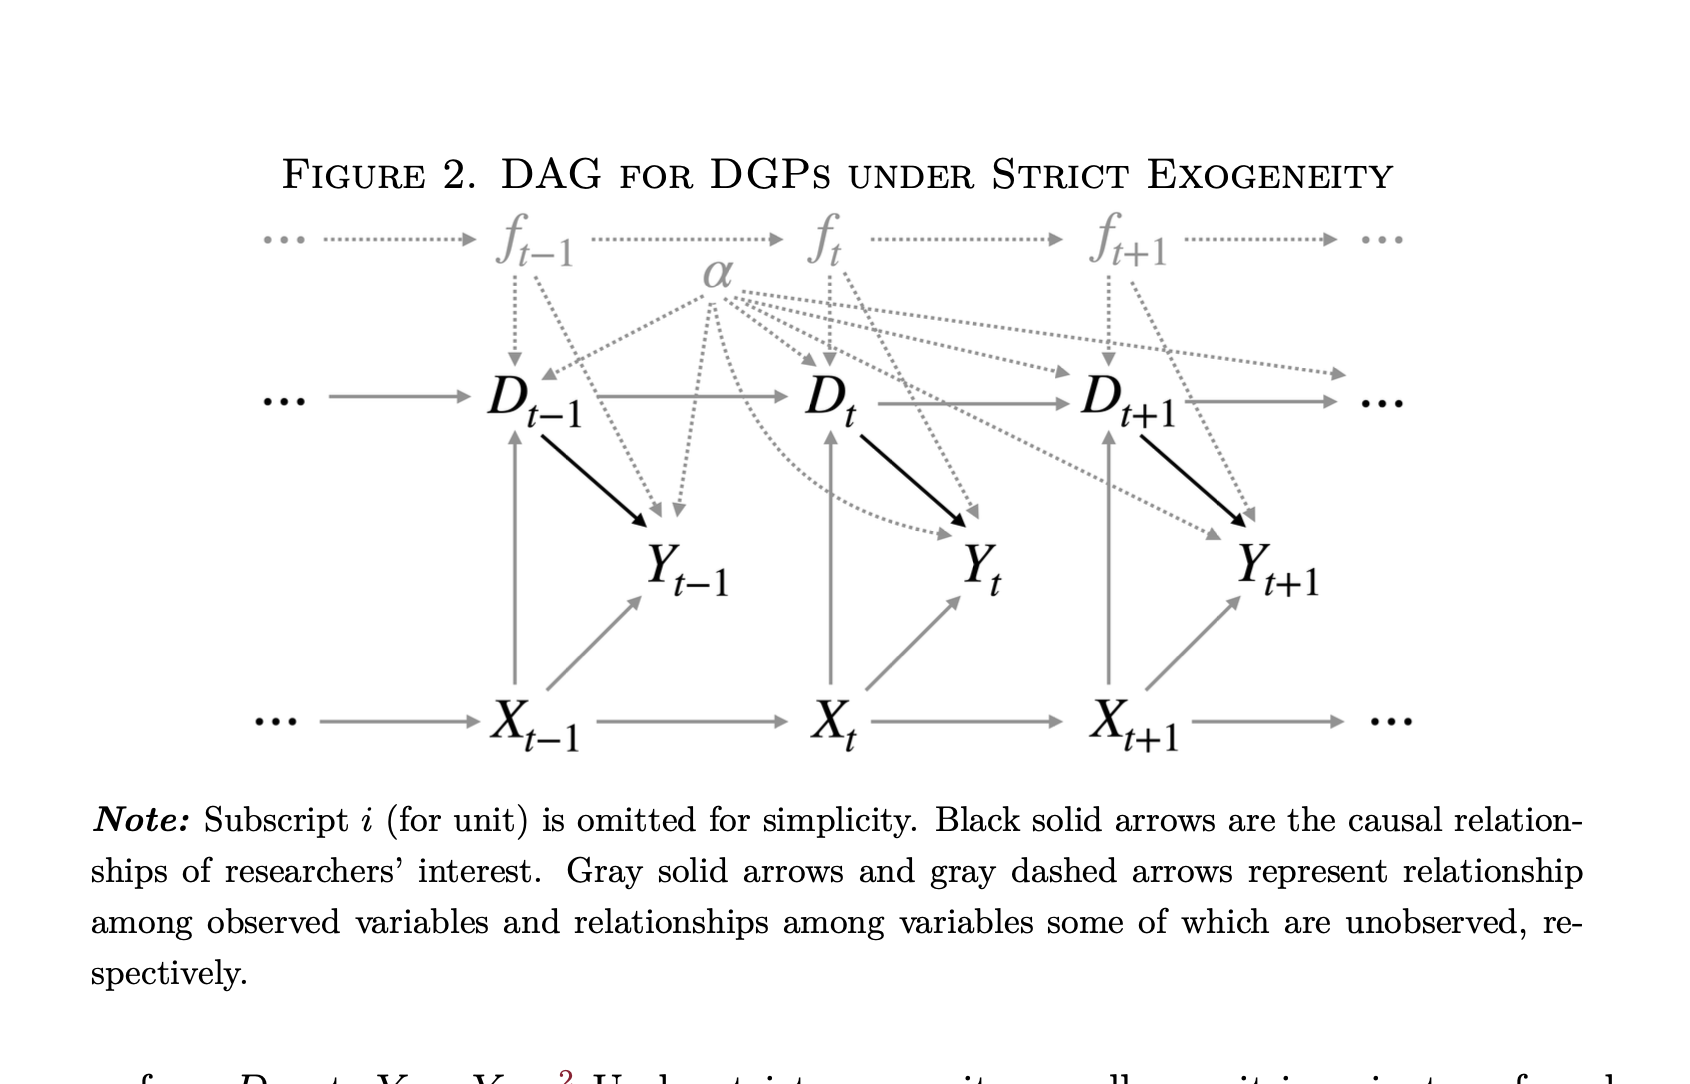
\includegraphics[width=23.47in]{imagens/DAG estrita exogeneidade} \caption{Exogeneidade estrita. O tratamento em cada período não pode responder a choques passados do outcome nem antecipar choques futuros; por isso, a hipótese exclui feedback dinâmico entre resultado e tratamento.}\label{fig:strict-exogeneity-dag}
\end{figure}

Em um modelo estático, exogeneidade estrita também se torna problemática quando o tratamento tem efeitos defasados omitidos. Se \(x_{i,t-1}\) afeta \(y_{it}\), mas o modelo inclui apenas \(x_{it}\), parte do efeito passado fica no erro. Como tratamentos são frequentemente persistentes, esse erro pode estar correlacionado com o tratamento presente.

\subsubsection{Ignorabilidade sequencial}\label{ignorabilidade-sequencial}

Ignorabilidade sequencial relaxa a ideia de que o tratamento não pode responder ao passado. O experimento imaginário é diferente: em cada período, o tratamento é atribuído condicionalmente à história observada da unidade.

Defina a história observada antes do tratamento em \(t\) como:
\[
H_{it} = (\bar{Y}_{i,t-1}, \bar{A}_{i,t-1}, \bar{X}_{it}).
\]
Aqui, \(H_{it}\) contém outcomes passados, tratamentos passados e covariáveis observadas até o momento da decisão de tratamento.

Se \(A_{it}\) é o tratamento no período \(t\) e \(\bar{a}\) é uma trajetória completa de tratamento, a suposição pode ser escrita como:
\[
A_{it}
\perp
\{Y_{is}(\bar a): s\geq t,\ \bar a\in\mathcal A^T\}
\mid H_{it}.
\]

Em palavras, dado tudo que observei até antes da atribuição do tratamento em \(t\), o tratamento atual é independente dos resultados potenciais futuros. Isso permite que tratamento dependa de resultados passados observados. Um município pode receber uma política porque teve baixo desempenho no ano anterior. A suposição exige que, depois de condicionar nesse histórico observado, não reste confusão não observada que afete tanto o tratamento quanto os resultados potenciais.

No caso simples de um tratamento após o período pré, essa hipótese se aproxima de:
\[
D_i \perp \{Y_{i1}(0),Y_{i1}(1)\}\mid Y_{i0},X_i.
\]

Essa é uma hipótese de seleção em observáveis. Ela é diferente de PT. PT pode valer quando ignorabilidade em níveis falha, porque DiD remove diferenças fixas de nível. E ignorabilidade condicional pode valer sem que PT incondicional valha, porque tratados e controles podem ter diferentes valores iniciais e regressão à média.

O DAG abaixo ilustra a suposição de ignorabilidade sequencial.

\begin{figure}
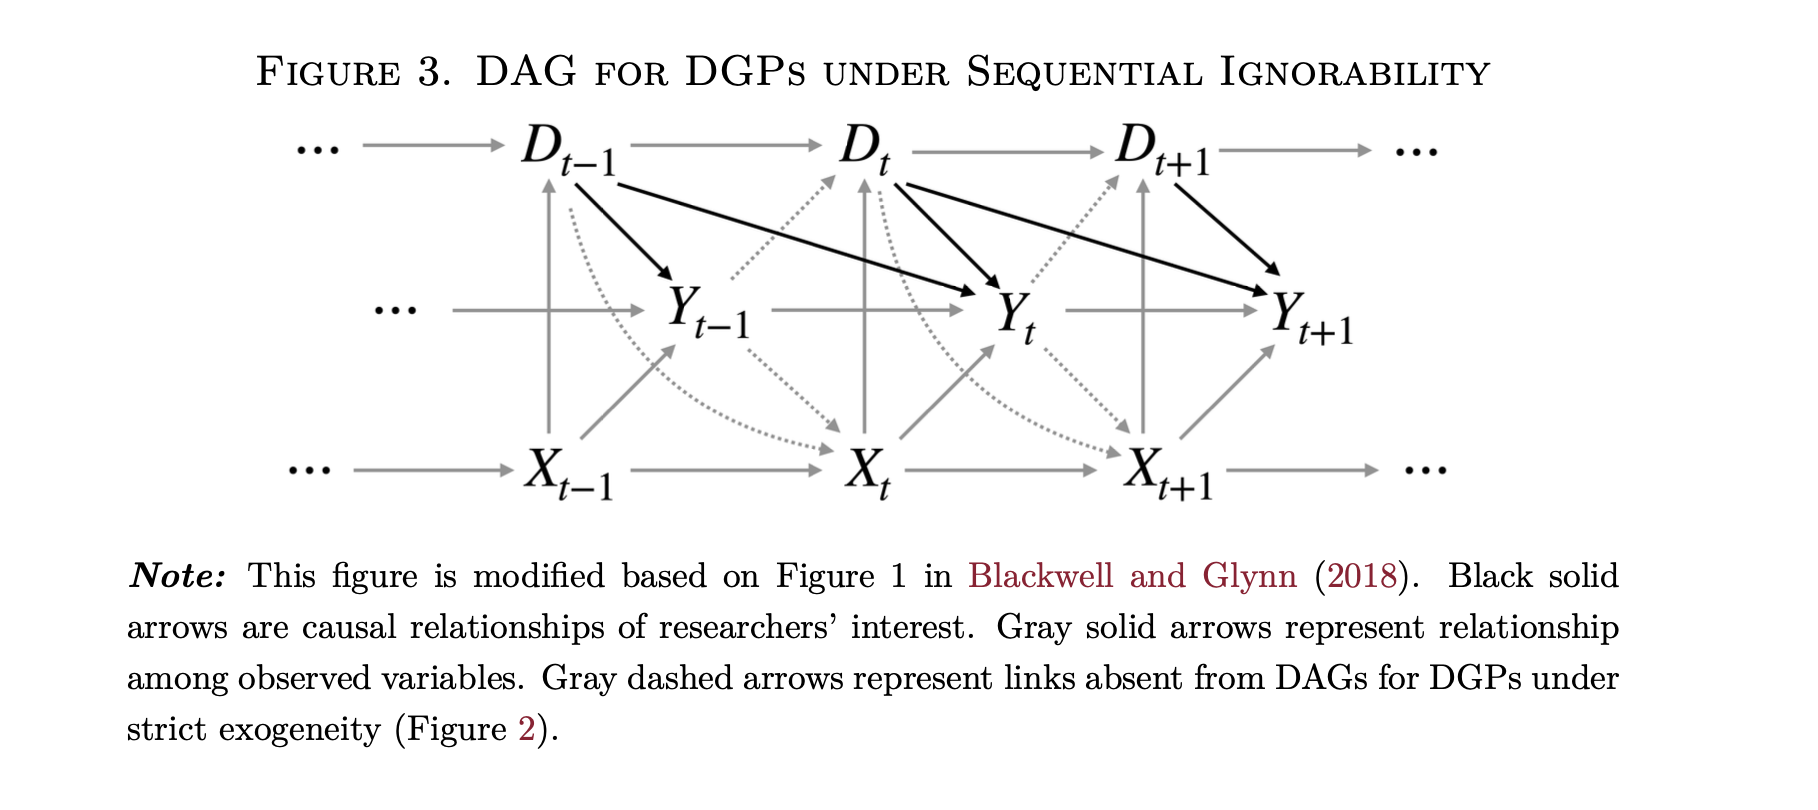
\includegraphics[width=25.25in]{imagens/sequential ignorability} \caption{Ignorabilidade sequencial. O tratamento pode responder à história observada; a hipótese exige que, após condicionar nessa história, não reste confusão não observada para os resultados potenciais futuros.}\label{fig:sequential-ignorability-dag}
\end{figure}

Essa suposição costuma exigir estimadores próprios, como modelos marginais estruturais, IPW, g-formula ou métodos relacionados. Incluir controles contemporâneos em uma regressão TWFE nem sempre resolve o problema, especialmente se esses controles foram afetados por tratamentos passados.

\subsubsection{TWFE, FE e RE nessa linguagem}\label{twfe-fe-e-re-nessa-linguagem}

A regressão TWFE é:
\[
Y_{it}=\alpha_i+\lambda_t+\tau A_{it}+u_{it}.
\]

Uma leitura em resultados potenciais é:
\[
Y_{it}(0)=\alpha_i+\lambda_t+u_{it}(0),
\]
e, se o efeito for constante:
\[
Y_{it}(1)=Y_{it}(0)+\tau.
\]

Para interpretar \(\tau\) causalmente, precisamos de uma condição sobre o erro do resultado não tratado. Em linguagem de regressão, isso se parece com:
\[
\mathbb{E}[u_{it}(0)\mid A_{i1},\ldots,A_{iT},\alpha_i,\lambda_t]=0.
\]

Em linguagem de DiD, isso se parece mais com PT no resíduo:
\[
\mathbb{E}[u_{it}(0)-u_{is}(0)\mid \text{tratados}]
=
\mathbb{E}[u_{it}(0)-u_{is}(0)\mid \text{controles}].
\]

TWFE incorpora a intuição do DiD porque remove \(\alpha_i\) e \(\lambda_t\). Mas o coeficiente TWFE só tem interpretação causal simples sob condições adicionais, como ausência de antecipação, especificação correta da comparação, e cuidado com heterogeneidade de efeitos em desenhos escalonados.

Efeitos fixos permitem que a heterogeneidade fixa da unidade esteja correlacionada com o tratamento:
\[
D_i \not\perp \alpha_i.
\]

Essa é justamente sua vantagem em relação a efeitos aleatórios. Em efeitos aleatórios, em geral assumimos algo mais forte:
\[
\mathbb{E}[\alpha_i\mid \bar A_i,\bar X_i]=\mathbb{E}[\alpha_i].
\]

Ou seja, a heterogeneidade não observada fixa da unidade não pode estar correlacionada com a trajetória de tratamento. Para identificação causal em painel, FE conversa naturalmente com PT; RE conversa mais naturalmente com uma hipótese de ausência de seleção na heterogeneidade não observada.

\subsection{Modelos dinâmicos e feedback}\label{modelos-dinuxe2micos-e-feedback}

A distinção entre exogeneidade estrita e ignorabilidade sequencial fica clara quando pensamos em modelos dinâmicos.

Considere um Distributed Lag Model (DLM), que inclui valores defasados do tratamento:
\[
y_{it} = \alpha + \beta_1 x_{it} + \beta_2 x_{i,t-1} + \cdots + \beta_k x_{i,t-k} + e_{it}.
\]

Um modelo relacionado é o ADL, \emph{autoregressive distributed lag}, que inclui a variável dependente defasada:
\[
y_{it} = \alpha + \alpha_1 y_{i,t-1} + \beta_1 x_{it} + \beta_2 x_{i,t-1} + e_{it}.
\]

A equação de resultados potenciais implicada por esse modelo pode ser escrita como:
\[
Y_{it}(x_{i,1:t}) =
\alpha + \alpha_1 Y_{i,t-1}(x_{i,1:t-1})
+ \beta_1x_{it} + \beta_2 x_{i,t-1} + e_{it}.
\]

Essa formulação mostra por que a interpretação causal de \(x_{i,t-1}\) é difícil. O tratamento passado pode ter efeito direto sobre \(y_{it}\), via \(\beta_2\), e efeito indireto via \(y_{i,t-1}\).

Agora considere o modelo AR(1):
\[
y_t = \beta_0 + \beta_1 y_{t-1} + e_t.
\]

Suponha que:
\[
\mathbb{E}[e_t \mid y_{t-1}, y_{t-2}, \ldots] = 0.
\]

Então:
\[
\mathbb{E}[y_t \mid y_{t-1}, y_{t-2}, \ldots]
= \beta_0 + \beta_1 y_{t-1}.
\]

Como \(y_t\) contém \(e_t\), o erro atual está mecanicamente relacionado ao resultado atual. Quando modelos de painel incluem variável dependente defasada e efeitos fixos, surgem problemas adicionais, especialmente com \(T\) pequeno. A lição substantiva para esta aula é mais simples: dinâmica e feedback exigem que o pesquisador seja explícito sobre o pressuposto de identificação.

\subsection{Suposições para inferência}\label{suposiuxe7uxf5es-para-inferuxeancia}

Identificação não resolve inferência. Para calcular erros-padrão e fazer testes de hipótese, precisamos lidar com dependência serial e agrupamento.

\subsubsection{Correlação serial}\label{correlauxe7uxe3o-serial}

Em painéis, erros da mesma unidade em períodos diferentes costumam ser correlacionados:
\[
\operatorname{Corr}(u_{it}, u_{is} \mid X_i) \neq 0
\quad \text{para } t \neq s.
\]

Correlação serial afeta principalmente o cálculo dos erros-padrão. Ela não cria, por si só, viés no coeficiente. Mas, se ignoramos essa dependência, a incerteza estimada tende a ser pequena demais. Bertrand, Duflo, and Mullainathan (\citeproc{ref-bertrand2004}{2004}) mostram isso de forma clara para DiD: em painéis com muitos anos, outcomes persistentes e tratamentos que também permanecem ligados após a adoção, erros-padrão convencionais podem rejeitar a hipótese nula com frequência muito maior do que deveriam. O problema não é que o coeficiente esteja necessariamente errado. O problema é que estamos contando como informação independente observações que, na prática, carregam choques parecidos ao longo do tempo.

A regra prática é clusterizar no nível em que a variação de tratamento é atribuída ou no nível em que os choques estão correlacionados. Se a política varia por município, clusterize por município. Se a política varia por estado, clusterize por estado. Se o tratamento é nacional e varia apenas no tempo, o problema é mais difícil: há pouca variação independente para inferência causal.

Há, porém, um caso em que correlação serial também pode sinalizar problema causal. Suponha que um choque negativo em \(y_{i,t-1}\) aumente a probabilidade de uma política em \(t\). Se os erros são serialmente correlacionados, esse choque passado também está relacionado ao erro em \(t\). O tratamento passa então a responder a um componente do outcome que continua afetando o outcome futuro. Um exemplo simples: municípios recebem intervenção porque tiveram uma piora fiscal no ano anterior, e essa piora fiscal tende a persistir. Comparar esses municípios com outros sem modelar essa regra de seleção pode atribuir à política uma trajetória que já teria sido diferente mesmo sem tratamento.

Nesse caso, o problema não é apenas o erro-padrão. A exogeneidade estrita falha, porque \(x_{it}\) responde a choques passados de \(y\). Tendências paralelas também ficam ameaçadas, pois tratados e controles podem ter tendências contrafactuais diferentes depois do choque. A ignorabilidade sequencial é uma alternativa conceitual: ela permite que o tratamento responda ao passado observado, mas exige condicionar adequadamente na história que determina a atribuição do tratamento.

\subsubsection{Raiz unitária}\label{raiz-unituxe1ria}

Uma segunda fonte de persistência é a raiz unitária. A intuição é simples. Em uma série sem raiz unitária, choques têm efeito temporário: depois de algum tempo, a série tende a voltar para sua trajetória ou média. Em uma série com raiz unitária, choques têm efeito permanente. O exemplo canônico é:
\[
y_t = y_{t-1} + e_t.
\]

Nesse processo, um choque em \(e_t\) altera não apenas \(y_t\), mas também o ponto de partida de todos os períodos seguintes. A série passa a ter uma tendência estocástica. Por isso, regressões em níveis com séries que têm raiz unitária podem produzir relações aparentemente fortes apenas porque as séries se movem persistentemente ao longo do tempo. Aqui, de novo, o primeiro problema é de inferência e especificação: erros-padrão usuais e testes convencionais podem ser enganosos, e pode ser necessário trabalhar com diferenças, tendências, modelos dinâmicos ou diagnósticos específicos de série temporal.

A raiz unitária também pode virar problema causal quando o tratamento responde a choques passados do outcome. Se um choque permanente em \(y\) aumenta a probabilidade de tratamento no período seguinte, os tratados entram no pós-tratamento em uma trajetória contrafactual diferente. Por exemplo, imagine que um município recebe uma política depois de uma queda permanente na arrecadação. Mesmo sem a política, sua trajetória futura de arrecadação já seria diferente da trajetória dos municípios não tratados. Isso ameaça PT. Para defender ignorabilidade sequencial, seria preciso argumentar que a história observada, incluindo o nível e a trajetória recente do outcome, captura a regra de atribuição do tratamento.

\subsection{Resumo}\label{resumo-1}

A ideia do capítulo é que efeitos fixos definem comparações. Eles removem variação e deixam o coeficiente ser estimado com o que sobra.

\begin{table}

\caption{\label{tab:checklist-final-painel}Checklist final para interpretar modelos de painel com efeitos fixos.}
\centering
\begin{tabular}[t]{l|l}
\hline
Dimensão & Pergunta\\
\hline
Unidade-tempo & Qual é a unidade e qual é o período?\\
\hline
Variação residual & Qual variação identifica o coeficiente depois dos efeitos fixos?\\
\hline
Tratamento & O tratamento é binário, contínuo, acumulado ou uma história?\\
\hline
Identificação & Qual pressuposto sustenta a interpretação causal?\\
\hline
Inferência & O erro-padrão reconhece o nível correto de dependência nos dados?\\
\hline
\end{tabular}
\end{table}

O DAG abaixo resume diferentes regimes de identificação.

\begin{figure}
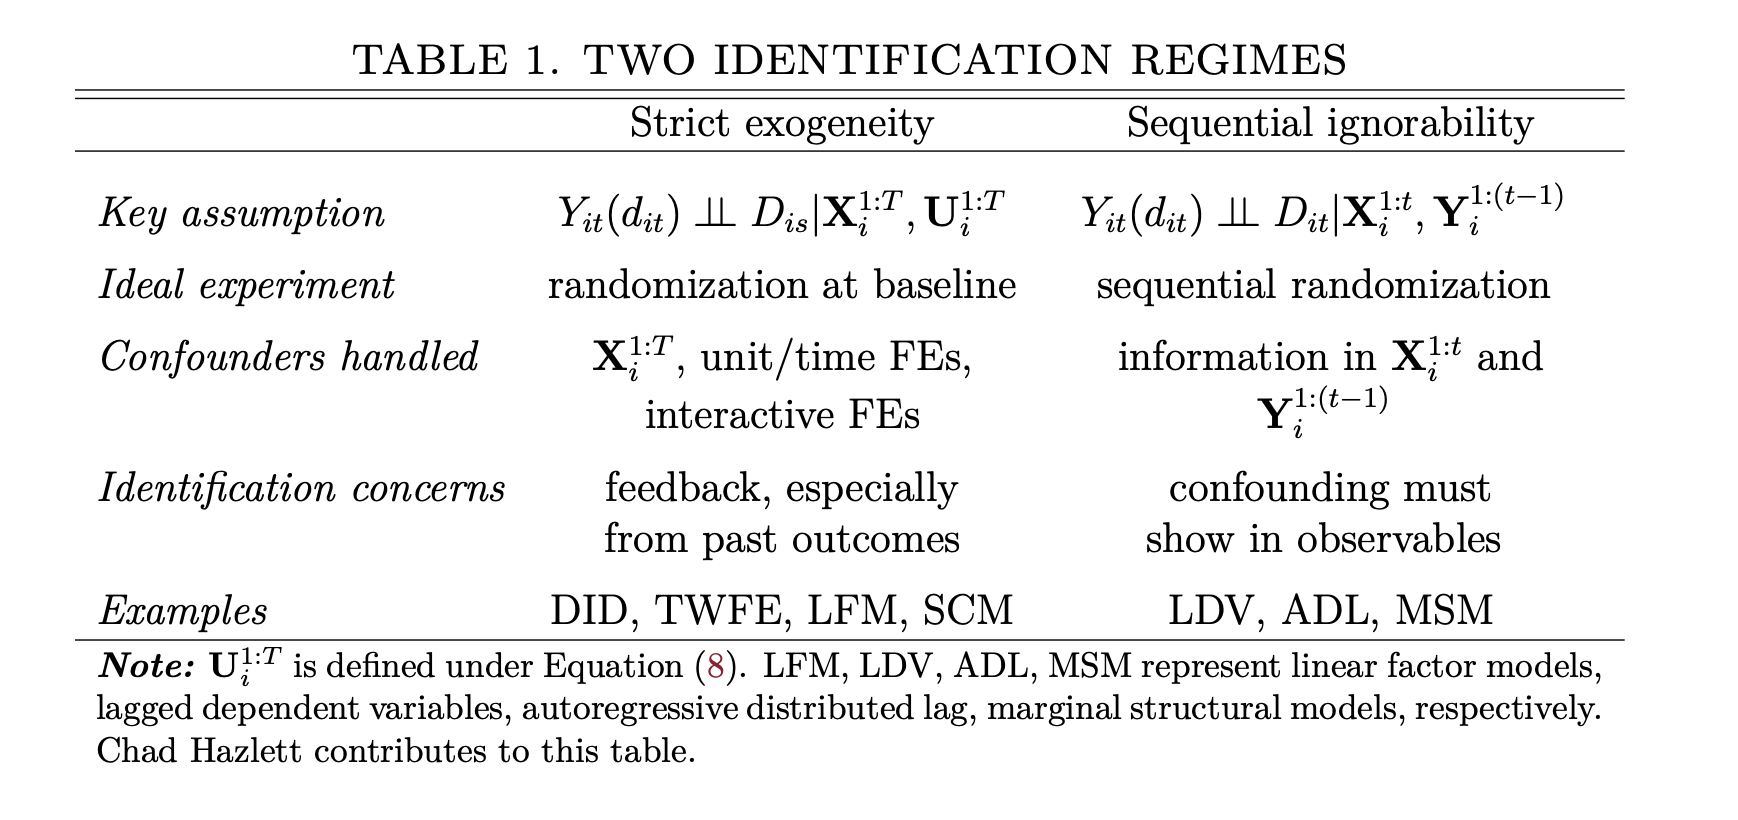
\includegraphics[width=24.14in]{imagens/identification regimes} \caption{Regimes de identificação. Use esta figura como mapa final: cada estimador só é interpretável causalmente depois que o pressuposto correspondente foi declarado e defendido.}\label{fig:identification-regimes-fig}
\end{figure}

\subsection{Referências}\label{referuxeancias-2}

Bell, A., \& Jones, K. (2015). Explaining fixed effects: Random effects modeling of time-series cross-sectional and panel data. Political Science Research and Methods, 3(1), 133-153.

Blackwell, M., \& Glynn, A. N. (2018). How to make causal inferences with time-series cross-sectional data under selection on observables. American Political Science Review, 112(4), 1067-1082.

Page, S. E. (2006). Path dependence. Quarterly Journal of Political Science, 1(1), 87-115.

\section{Interferência, spillover e dinâmica}\label{interferuxeancia-spillover-e-dinuxe2mica}

Agora iremos relaxar algumas simplificações do modelo de Resultados potenciais que vimos até agora.

\subsection{Suposições simplificadoras}\label{suposiuxe7uxf5es-simplificadoras}

\begin{enumerate}
\def\labelenumi{\arabic{enumi}.}
\tightlist
\item
  Tratamento binário
\item
  Único período de tempo (um tratamento ``within unit'')
\item
  SUTVA
\end{enumerate}

\subsection{PO com tratamento de múltiplos valores (multi-valued)}\label{po-com-tratamento-de-muxfaltiplos-valores-multi-valued}

\subsubsection{Multi-valued discreto}\label{multi-valued-discreto}

Vamos estender o modelo de tratamento binário começando por tratamentos discretos. Digamos que temos \(D_i \in \{0, 1, ..., d\}\), isto é, tratamentos ordenados. Por exemplo, múltiplas categorias de uma política pública (100 reais, 200 reais, 300 reais etc.). Definimos o resultado potencial da unidade \(i\) para qualquer \(d \in D\) como \(Y_i(d)\).

Nós vamos precisar da suposição de ignorability forte.

\(\tau_i(D, D') = Y_i(d) - Y_i(d')\), ou seja, o efeito causal entre dois níveis do tratamento. Como antes, podemos computar a esperança: \(\mathbb{E}[\tau_i(D, D')] = \mathbb{E}[Y_i(d) - Y_i(d')]\). E se ignorability forte vale, então \(\mathbb{E}[\tau_i(D, D')] = \mathbb{E}[Y_i|D_i = d] - \mathbb{E}[Y_i|D_i = d']\)

Se quisermos, podemos trabalhar também com tratamentos não-ordenados. Por exemplo, dois tratamentos binários. Por exemplo, um tratamento é informação sobre corrupção de um candidato (recebe ou não a informação) e outro tratamento é informação sobre a raça do candidato (é branco ou não). \(D_i \in \{0,1\}^2\). Podemos modelar os resultados potenciais como dependendo do status dos dois tratamentos: \(Y_i(D_{i1}, D_{i2})\) que geram quatro possibilidades ou resultados potenciais: \(Y(0,0)\), \(Y(1,0)\), \(Y(0,1)\), \(Y(1,1)\).

Exemplo onde mesmo com atribuição aleatória, há efeitos não-identificados. Aleatoriamente atribuir \(D_1\) e, para os que receberam \(D_1\), aleatoriamente atribuir \(D_2\). Onde isso poderia acontecer? Primeira e segunda dose de vacina! Por definição, a segunda dose só é dada para quem recebeu a primeira dose. Nunca é possível estimar efeito relativo a \(Y_i(0,1)\), isto é, o resultado potencial de quem não recebeu a primeira dose, mas recebeu a segunda. Essa é uma pessoa que recebeu a primeira dose quando a segunda estava sendo aplicada.

\subsection{Dinâmica}\label{dinuxe2mica}

Considere que agora nós observamos \(T\) períodos de tempo para uma unidade: \(Y_i = (Y_{i1}, Y_{i2}, \ldots, Y_{iT})\). Para cada período, há um tratamento \(D_{it} \in \{0,1\}\), isto é, sempre binário. Chamamos de \(\mathbf{D_i} = (D_{i1}, D_{i2}, ..., D_{iT})\) o vetor de tratamentos em todos os \(T\) períodos. Implicitamente, muitas pessoas abordam modelos dinâmicos supondo que podemos olhar apenas para o resultado potencial para a unidade \(i\) no período \(t\), ou seja, \(Y_{it}(D_{it})\). Porém, isso significa que apenas o tratamento do período \(t\) impacta o resultado potencial do período \(t\). De maneira mais geral, teríamos: \(\mathbf{D_i} = (D_{i1}, D_{i2}, ..., D_{iT})\) e definiríamos o resultado potencial no período \(t\) como \(Y_{it}(\mathbf{D_i})\). \(Y(\mathbf{D})\). Nesse caso, fomos para o lado oposto: tratamentos futuros impactando o resultado potencial do presente. Isso não necessariamente significa que o futuro afeta o passado. Pode ocorrer por antecipação de tratamentos futuros. De todo modo, também parece extremo. Ainda assim, continuamos evitando a possibilidade de spillovers.

Uma suposição comum, portanto, é a de não-antecipação, que pode ser representada por: \(Y_{it}(d_1, d_2, ..., d_t, d_{t+1}, ..., d_T) = Y_{it}(d_1, d_2, ..., d_t)\). Ou seja, os resultados potenciais até \(t\) não dependem dos tratamentos após essa data.

Outra suposição comum é: ausência de efeitos dinâmicos:
\[Y_{it}(d_1, d_2, ..., d_t) = Y_{it}(d_t)\]
Em palavras, essa suposição requer que o resultado potencial do presente não dependa dos tratamentos passados. Essa suposição é também chamada de ``no carry-over-effects hypothesis''. Ela é bem restritiva. Mesmo um desenho em que a aleatorização é executada a cada período de maneira independente pode ter ``carry-over-effects'' se o resultado do período anterior impactar o resultado do período presente.

Modelos de ``impulse response function'' estão interessados em estimar justamente ``carry over effects''. ver \url{https://donskerclass.github.io/CausalEconometrics/TimeSeries.html}

Considere um modelo de regressão tradicional para dados dinâmicos: \(y_{it} = \alpha + \beta x_{it} + e_{it}\). Nós já sabemos que uma forma de pensar a identificação causal é imaginar um experimento aleatório controlado. O que significa, em primeiro lugar, escolher aleatoriamente o tratamento nesse caso? Uma possibilidade é imaginar que a cada período o tratamento é aleatoriamente atribuído, independentemente dos períodos anteriores. No fundo, é como um \emph{multi-valued treatment}. Qual condição de ignorability estamos satisfazendo nesse caso? Se apenas o tratamento presente impacta o resultado potencial, isto é, \(Y_{it}(D_{it})\), então temos:

\begin{enumerate}
\def\labelenumi{\arabic{enumi}.}
\item
  Baseline randomization: \(Y(D_{it}) \perp D_{it}\). Ou seja, o resultado potencial no período \(t\) é independente do mecanismo de atribuição do tratamento. Essa suposição implica exogeneidade estrita.
\item
  Ignorability sequencial (Sequential Unconfoundedness). Assume que, conditional à história passada observada de tratamentos e covariáveis, o tratamento corrente é independente de resultados potenciais.
\end{enumerate}

Nós iremos aprofundar essas questões nas aulas sobre DiD e Efeitos Fixos. Por ora, quero notar que no fundo estamos falando de spillovers no tempo, isto é, tratamento no tempo \(t\) impactando resultados potenciais de períodos futuros \(t+(1:k)\), em que \(k >0\).

\subsection{Interferência}\label{interferuxeancia}

Interferência ocorre quando o resultado potencial de uma unidade depende do tratamento de outra unidade. Tipicamente, em ciências sociais, spillovers podem envolver:

\begin{enumerate}
\def\labelenumi{\arabic{enumi}.}
\item
  Efeitos de pares
\item
  Spillovers espaciais
\item
  Interações políticas (restrições orçamentárias)
\end{enumerate}

Para modelar interferência, é necessário enriquecer nosso framework, introduzindo definições adicionais e alterando os pressupostos chave. Tipicamente nós modelamos com a suposição de que a interferência ocorre apenas em um subgrupo de unidades, isto é, o resultado potencial não depende do status de tratamento de todas as unidades, mas tão somente de um grupo específico. Além disso, também é comum ser necessária a suposição de anonimidade, isto é, os pares de um grupo importam, mas não quem são os pares, no sentido de que cada par teria um efeito específico e único sobre uma unidade. Essa é uma área de pesquisa ativa na inferência causal, mas ainda pouco incorporada na ciência política, em particular nas RIs, mas não só.

Referências chave são:
Charles F Manski. Identification of treatment response with social interactions. The Econometrics Journal, 16(1):S1--S23, 2013.

Peter M Aronow and Cyrus Samii. Estimating average causal effects under general interference, with application to a social network experiment. Annals of Applied Statistics, 11(4):1912--1947, 2017.

Bowers J, Fredrickson MM, Panagopoulos C. Reasoning about Interference Between Units: A General Framework. Political Analysis. 2013;21(1):97-124. \url{doi:10.1093/pan/mps038}

\section{Controle Sintético e Estimação Contrafactual}\label{controle-sintuxe9tico-e-estimauxe7uxe3o-contrafactual}

\textbf{Objetivos de aprendizado.} Ao final deste capítulo, o leitor será capaz de:

\begin{enumerate}
\def\labelenumi{\arabic{enumi}.}
\tightlist
\item
  Explicar como regressão e SCM imputam contrafactuais a partir dos controles, distinguindo pesos implícitos de pesos convexos explícitos.
\item
  Implementar o SCM no R e interpretar seus resultados (pesos, balanço de preditores, gráficos de gap).
\item
  Avaliar criticamente a inferência por permutação do SCM, incluindo suas limitações quando o tratamento não é aleatorizado.
\item
  Distinguir entre modelos aditivos (FEct/DiD) e modelos de fatores (IFEct/MC), e entender quando cada um é apropriado.
\item
  Explicar como o SCM motiva modelos de fatores, e por que estimar fatores diretamente pode ser mais eficiente quando há múltiplas unidades tratadas.
\item
  Comparar DiD, SCM, SDiD e TROP em termos de suposições, flexibilidade e robustez, e escolher o método adequado para uma aplicação concreta.
\end{enumerate}

\subsection{Motivação}\label{motivauxe7uxe3o}

No capítulo 8, vimos que o DiD requer tendências paralelas: na ausência de tratamento, tratados e controles teriam evoluído de forma similar. Mas essa suposição é frequentemente violada --- especialmente quando há poucas unidades tratadas (às vezes apenas uma) ou quando confundidores variam no tempo de forma heterogênea entre grupos.

Este capítulo apresenta uma família de métodos que compartilham a mesma lógica: \textbf{imputar o contrafactual} \(Y_{it}(0)\) para as observações tratadas. A diferença entre eles está no \emph{modelo} que usam para essa imputação e nas \emph{restrições} que impõem:

\begin{itemize}
\tightlist
\item
  O \textbf{Controle Sintético} (SCM) constrói o contrafactual como combinação convexa de unidades não-tratadas.
\item
  O \textbf{framework de estimação contrafactual} (Liu, Wang \& Xu, 2024) generaliza a imputação para três estimadores --- FEct, IFEct e MC --- com diagnósticos formais.
\item
  O \textbf{Synthetic DiD} (Arkhangelsky et al., 2021) combina pesos de unidade (como SCM) com pesos temporais e efeitos fixos (como DiD).
\item
  O \textbf{TROP} (Athey et al., 2025) combina um modelo de fatores com pesos de unidade e pesos temporais, obtendo tripla robustez.
\end{itemize}

\textbf{Mapa do capítulo.} As seções 2--3 cobrem o SCM clássico e sua implementação no R. A seção 4 introduz o framework de estimação contrafactual. A seção 5 apresenta os três estimadores (FEct, IFEct, MC) com aplicação empírica. A seção 6 discute diagnósticos. A seção 7 apresenta o Synthetic DiD. A seção 8 introduz o TROP. A seção 9 oferece um guia prático de escolha entre métodos. A seção 10 resume o capítulo.

\subsection{Controle Sintético clássico}\label{controle-sintuxe9tico-cluxe1ssico}

O método de controle sintético foi originalmente proposto por Abadie e Gardeazabal (2003) para estimar os custos econômicos do conflito no País Basco, e posteriormente formalizado e popularizado por Abadie, Diamond e Hainmueller (2010, 2015). A intuição aparece com clareza no exemplo clássico da Proposição 99. A Califórnia aprovou em 1988 uma política ampla de controle do tabaco. Queremos estimar seu efeito sobre as vendas per capita de cigarros:

\[
\tau_t = Y_{CA,t}(1) - Y_{CA,t}(0), \quad \text{para } t > 1988
\]

O termo observado é \(Y_{CA,t}(1)\), a trajetória da Califórnia após a política. O termo que falta é \(Y_{CA,t}(0)\), a trajetória que a Califórnia teria seguido sem a Proposição 99. Esse contrafactual não está nos dados. Todo o problema é construir uma estimativa crível de \(Y_{CA,t}(0)\) usando os estados que não adotaram a política.

\begin{table}

\caption{\label{tab:cigarro}Primeiras observações dos dados de vendas de cigarros.}
\centering
\begin{tabular}[t]{l|r|r|l}
\hline
state & year & cigsale & california\\
\hline
Rhode Island & 1970 & 123.9 & FALSE\\
\hline
Tennessee & 1970 & 99.8 & FALSE\\
\hline
Indiana & 1970 & 134.6 & FALSE\\
\hline
Nevada & 1970 & 189.5 & FALSE\\
\hline
Louisiana & 1970 & 115.9 & FALSE\\
\hline
Oklahoma & 1970 & 108.4 & FALSE\\
\hline
\end{tabular}
\end{table}

\begin{figure}
\centering
\pandocbounded{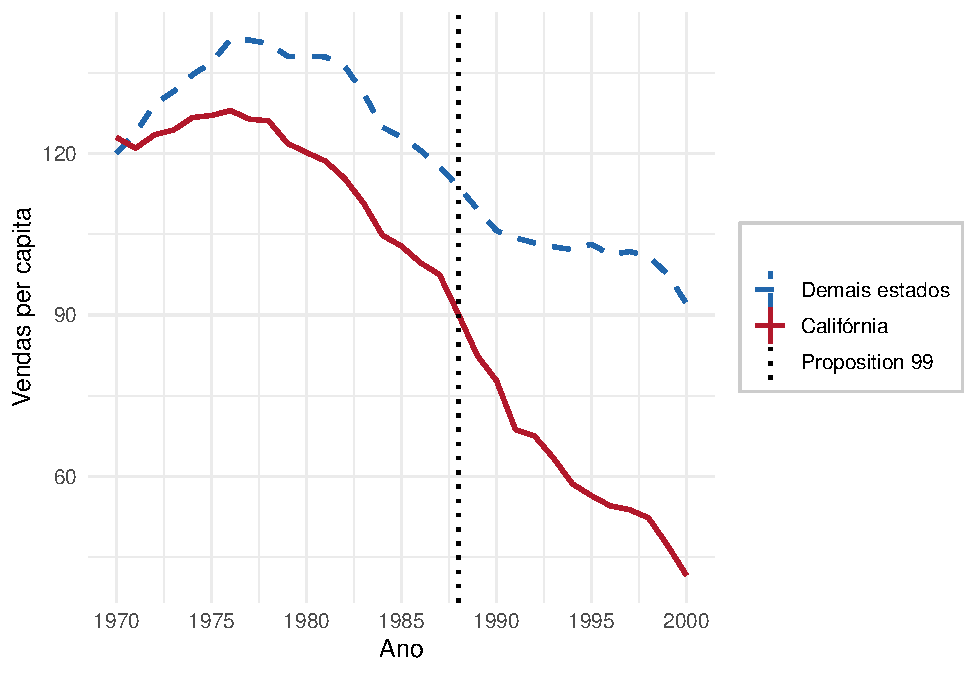
\includegraphics[keepaspectratio,alt={\label{fig:cigarro}Vendas per capita de cigarros na Califórnia e nos demais estados. A linha vertical marca a aprovação da Proposição 99 em 1988.}]{bookdownproj_files/figure-latex/cigarro-1.pdf}}
\caption{\label{fig:cigarro}Vendas per capita de cigarros na Califórnia e nos demais estados. A linha vertical marca a aprovação da Proposição 99 em 1988.}
\end{figure}

A média simples dos demais estados não é um bom contrafactual. Os controles diferem da Califórnia em nível e tendência antes de 1988. Uma primeira saída natural é usar regressão: estimar, entre os estados não tratados, uma relação entre características pré-tratamento e o resultado futuro, e depois aplicar essa relação à Califórnia.

\subsubsection{Regressão como primeira tentativa de contrafactual}\label{regressuxe3o-como-primeira-tentativa-de-contrafactual}

Considere uma regressão estimada apenas no \emph{donor pool}. Para cada estado de controle, construímos um vetor de preditores pré-tratamento, incluindo valores defasados de vendas de cigarros e covariáveis como renda, preço relativo e composição etária. Para fixar a ideia, suponha que queremos prever as vendas per capita em 2000:

\[
\text{cigsale}_{j,2000}
= \alpha
+ \beta_{1970}\text{cigsale}_{j,1970}
+ \cdots
+ \beta_{1988}\text{cigsale}_{j,1988}
+ Z'_j\gamma
+ u_j,
\quad j \in co.
\]

Aqui, \(co\) denota o conjunto de estados de controle.

Depois de estimar o modelo nos controles, inserimos os preditores da Califórnia e obtemos \(\widehat{Y}_{CA,2000}(0)\). Essa operação parece diferente do SCM, mas também constrói o contrafactual como uma combinação linear dos estados de controle.

Defina \(X\) como a matriz de preditores dos estados de controle, incluindo a constante, \(y\) como o vetor de resultados dos controles em 2000, e \(x_{CA}\) como o vetor de preditores da Califórnia. A regressão produz:

\[
\widehat{\beta} = (X'X)^{-1}X'y.
\]

A previsão para a Califórnia é:

\[
\widehat{Y}_{CA,2000}(0)
= x_{CA}'\widehat{\beta}
= x_{CA}'(X'X)^{-1}X'y.
\]

Agrupando os termos que multiplicam \(y\), temos:

\[
h_{CA} = x_{CA}'(X'X)^{-1}X',
\]

e portanto:

\[
\widehat{Y}_{CA,2000}(0)
= h_1Y_{1,2000} + h_2Y_{2,2000} + \cdots + h_JY_{J,2000}.
\]

O vetor \(h_{CA}\) é uma linha \emph{out-of-sample} análoga à \emph{hat matrix}. Cada elemento de \(h_{CA}\) é o peso de um estado de controle no contrafactual por regressão. Com intercepto, esses pesos somam 1. A diferença é que a regressão não exige que sejam positivos, menores que 1 ou concentrados em poucos doadores.

\begin{table}

\caption{\label{tab:tabela-pesos-regressao-scm}Resumo dos pesos usados pelo SCM e dos pesos implícitos da regressão no exemplo da Califórnia.}
\centering
\begin{tabular}[t]{l|r|r|r|r|r|r}
\hline
Método & Soma dos pesos & Peso mínimo & Peso máximo & Pesos negativos & Pesos efetivos & Norma L1\\
\hline
SCM & 1 & 0.000 & 0.342 & 0 & 5 & 1.00\\
\hline
Regressão OLS & 1 & -0.325 & 0.493 & 17 & 38 & 3.96\\
\hline
\end{tabular}
\end{table}

A tabela mostra o ponto de Abadie e L'Hour (2021). A regressão também usa os controles como uma combinação ponderada. No exemplo, os pesos implícitos da OLS somam 1, mas 17 são negativos e todos os 38 estados entram com peso efetivo. O SCM também soma 1, mas não tem pesos negativos e concentra peso em cinco doadores. Entre os maiores pesos em valor absoluto da regressão estão Connecticut, Montana e Utah com pesos positivos, e Mississippi e Oklahoma com pesos negativos.

\begin{figure}
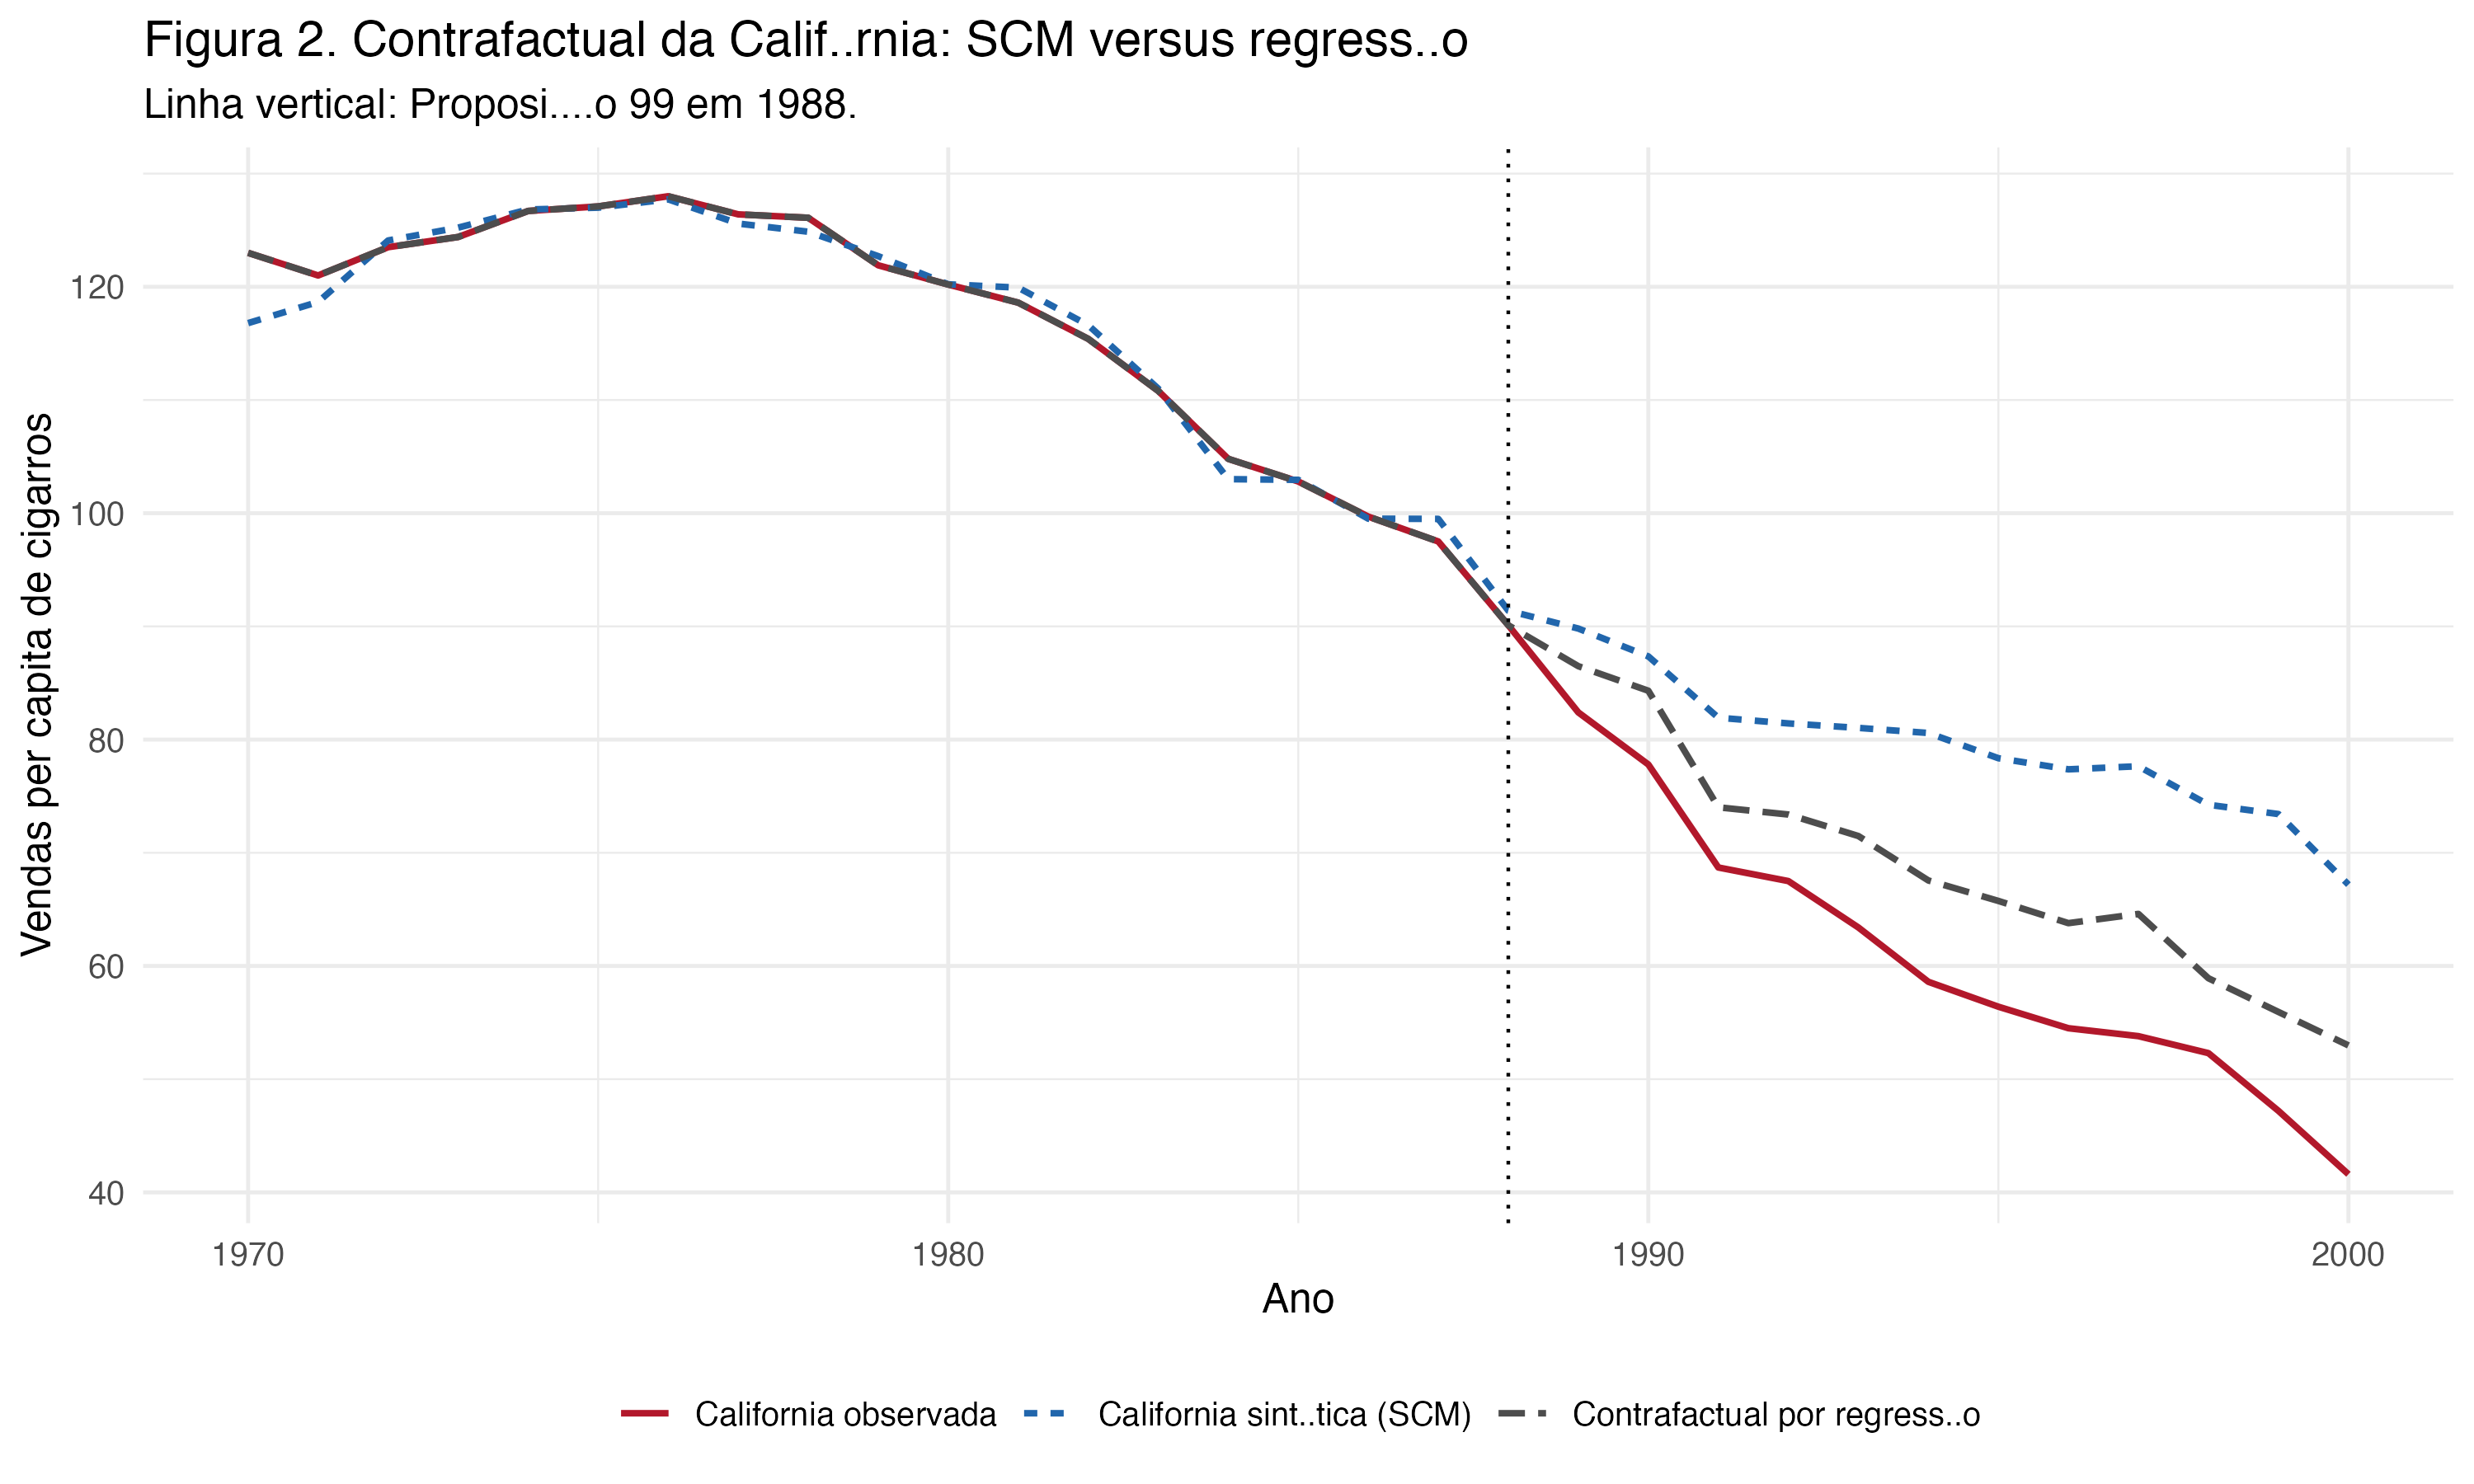
\includegraphics[width=0.95\linewidth]{outputs/scm_vs_regressao_prop99/figura_2_contrafactual_scm_vs_regressao} \caption{Califórnia observada, contrafactual por regressão e controle sintético. A linha vertical marca a Proposição 99 em 1988.}\label{fig:figura-contrafactual-scm-regressao}
\end{figure}

Em 2000, a Califórnia observada vendeu 41.6 maços per capita. A regressão prevê 53 e o SCM prevê 67.2. A comparação não prova que um estimador domina o outro. Ela mostra que contrafactuais com bom ajuste pré-tratamento podem ser produzidos por objetos substantivamente diferentes.

Na figura, a série por regressão usa o mesmo vetor \(h_{CA}\) para todos os anos. Isso corresponde a manter o mesmo conjunto de preditores e mudar apenas o resultado a ser previsto. Como esses preditores incluem muitas defasagens pré-tratamento, o bom ajuste no pré deve ser lido como diagnóstico descritivo, não como validação fora da amostra.

O problema não é apenas verificar se o ajuste pré-tratamento é bom. Isso vale para regressão, SCM e métodos posteriores. A pergunta mais difícil é que tipo de contrafactual gerou esse ajuste. Três riscos aparecem:

\begin{enumerate}
\def\labelenumi{\arabic{enumi}.}
\tightlist
\item
  \textbf{Confundimento dinâmico.} Se a Califórnia difere dos controles em fatores que afetam \(Y(0)\) e esses fatores não estão nos preditores, a previsão por regressão pode errar mesmo quando o ajuste observado parece razoável.
\item
  \textbf{Extrapolação funcional.} A regressão depende da forma funcional estimada nos controles. Quando a Califórnia está fora do suporte empírico dos controles, a previsão pode extrapolar além das comparações observadas.
\item
  \textbf{Baixa auditabilidade substantiva.} Pesos negativos e não esparsos dificultam a interpretação. A ``Califórnia da regressão'' pode somar alguns estados e subtrair outros. Essa construção é legítima como álgebra, mas é difícil de defender qualitativamente como unidade comparável.
\end{enumerate}

\subsubsection{O SCM como restrição disciplinadora}\label{o-scm-como-restriuxe7uxe3o-disciplinadora}

O SCM parte do mesmo problema, mas restringe a classe de contrafactuais admissíveis. Em vez de deixar a regressão escolher pesos implícitos sem restrição de sinal, o SCM constrói:

\[
\hat{Y}_{CA,t}(0) = \sum_{j \in co} w_jY_{j,t}
\]

com:

\[
w_j \geq 0
\qquad \text{e} \qquad
\sum_{j \in co} w_j = 1.
\]

Essas duas restrições forçam o contrafactual a ser uma combinação convexa explícita dos controles. Geometricamente, a Califórnia sintética precisa ficar dentro do \emph{convex hull} do \emph{donor pool}. Isso reduz extrapolação forte: o método tenta interpolar dentro do envelope empírico dos controles, em vez de projetar livremente a partir de uma forma funcional.

A analogia com \emph{matching} é útil. O SCM funciona como uma versão ponderada de \emph{nearest-neighbor matching}: procura controles parecidos com a unidade tratada, mas não impõe pesos iguais nem fixa previamente o número de vizinhos. A diferença é que a proximidade é definida pela capacidade de reproduzir a trajetória e os preditores pré-tratamento.

Essa disciplina tem custo. A convexidade pode ser rígida demais quando a unidade tratada está fora do \emph{convex hull} ou quando nenhuma combinação de controles ajusta bem o pré-tratamento. O SCM não é sempre melhor que regressão. Ele troca flexibilidade por transparência, auditabilidade e menor extrapolação.

\subsubsection{Formalização}\label{formalizauxe7uxe3o}

Suponha que temos dados para \(J+1\) unidades por \(T\) períodos: \(1, 2, \ldots, T_0, T_0+1, \ldots, T\). A primeira unidade (\(j=1\)) é tratada a partir de \(T_0+1\). As demais \(j = 2, \ldots, J+1\) formam o \emph{donor pool}. Para cada unidade, observamos um vetor de \(k\) preditores \(\mathbf{X}_j\), que pode incluir valores pré-intervenção da variável resposta.

Os dados podem ser organizados em blocos, onde as linhas representam períodos (pré e pós-tratamento) e as colunas representam unidades (controle e tratada):

\[
\begin{aligned}
D \;=\;
\underset{\text{linhas: períodos}}{\underbrace{
\begin{pmatrix}
\mathbf{0} & \mathbf{0}  \\
\mathbf{0} & \mathbf{1}
\end{pmatrix}
}}
\quad
\begin{matrix}
\leftarrow \text{pré} \\
\leftarrow \text{pós}
\end{matrix}
\qquad
Y \;=\;
\underset{\text{colunas: controle | tratada}}{\underbrace{
\begin{pmatrix}
Y_{co, pre}(0) & Y_{tr, pre}(0)  \\
Y_{co, post}(0)  & Y_{tr, post}(1)
\end{pmatrix}
}}
\end{aligned}
\]

O estimando é o ATT para os períodos pós-tratamento:
\[
\tau_t = \mathbb{E}[Y_{it}(1) \mid D_{it}=1] - \mathbb{E}[Y_{it}(0) \mid D_{it}=1]
\]

O contrafactual é estimado como média ponderada do donor pool:
\[
\hat{Y}_{tr, t}(0) = \sum_{j \in co} w_j Y_{j,t}
\]

com as restrições:

\begin{enumerate}
\def\labelenumi{\arabic{enumi}.}
\tightlist
\item
  \(\sum_j w_j = 1\) (combinação convexa)
\item
  \(w_j \geq 0\), \(\forall j\) (pesos não-negativos)
\end{enumerate}

Os pesos são escolhidos para que o controle sintético reproduza bem a unidade tratada antes da intervenção. O principal diagnóstico de ajuste é o RMSPE (\emph{Root Mean Squared Prediction Error}) no período pré-tratamento:

\[
\operatorname{RMSPE}_{pre}(\mathbf{w}) =
\sqrt{
\frac{1}{T_0}
\sum_{t \leq T_0}
\left(Y_{tr,t} - \sum_{j \in co} w_j Y_{j,t}\right)^2
}.
\]

Na formulação de Abadie, Diamond e Hainmueller (2010), isso é implementado minimizando a distância entre os preditores da unidade tratada e a combinação ponderada dos controles:
\[
\hat{\mathbf{W}}(V) = \arg\min_{\mathbf{W}} (\mathbf{X}_{tr} - \mathbf{X}_{co}\mathbf{W})' V (\mathbf{X}_{tr} - \mathbf{X}_{co}\mathbf{W})
\]
onde \(\mathbf{X}\) inclui a variável dependente defasada como preditor, e \(V\) é uma matriz diagonal positiva semidefinida (\(k \times k\)) que atribui importância relativa a cada preditor. A escolha de \(V\) é feita por uma otimização aninhada (\emph{nested optimization}): no loop externo, \(V\) é escolhida para minimizar o RMSPE no período pré-tratamento; no loop interno, dado \(V\), os pesos \(\mathbf{W}\) são otimizados sob as restrições de não-negatividade e soma igual a 1. Isso significa que os resultados do SCM dependem da escolha dos preditores incluídos em \(\mathbf{X}\) --- tanto a seleção quanto a ponderação dos preditores afetam a solução final.

\textbf{Por que o SCM funciona?} Sob um modelo linear de fatores \(Y_{it}(0) = \delta_t + \theta_t Z_i + \lambda_t \mu_i + \varepsilon_{it}\), onde \(Z_i\) são covariáveis observadas, \(\mu_i\) são fatores não-observados e \(\lambda_t\) são cargas temporais, Abadie, Diamond e Hainmueller (2010, Proposição 1) mostram que, se existem pesos que reproduzem exatamente os preditores pré-tratamento da unidade tratada (isto é, \(\mathbf{X}_{tr} = \mathbf{X}_{co}\mathbf{W}\)), então o viés do SCM desaparece quando \(T_0 \to \infty\). Intuitivamente, ao reproduzir as trajetórias pré-tratamento e as covariáveis observadas, o controle sintético também reproduz os fatores latentes não-observados --- que são a fonte de viés na ausência de tendências paralelas.

\textbf{Risco de sobreajuste.} Otimizar o ajuste pré-tratamento pode levar a \emph{overfitting}, especialmente quando se incluem todos os valores defasados da variável resposta como preditores. Kaul et al.~(2022) mostram que incluir todas as defasagens torna os demais preditores irrelevantes para a otimização. A recomendação prática é usar defasagens selecionadas (por exemplo, \(Y_{i,T_0}\), \(Y_{i,T_0/2}\)) e médias de covariáveis, em vez de todos os resultados pré-tratamento. O pesquisador deve justificar a escolha de preditores com base em conhecimento substantivo e verificar a robustez dos resultados a especificações alternativas (Abadie, 2021).

\textbf{Não-unicidade e viés de interpolação.} Um segundo problema, distinto do sobreajuste, é a \textbf{não-unicidade dos pesos}. Quando a unidade tratada está no interior do envoltório convexo (\emph{convex hull}) de muitos doadores, pode haver múltiplas combinações de pesos que reproduzem igualmente bem os dados pré-tratamento --- mas que divergem nas previsões pós-tratamento. Isso ocorre quando a informação pré-tratamento não identifica uma combinação única de doadores; com muitos doadores em relação aos preditores disponíveis, múltiplas soluções podem produzir o mesmo ajuste.

Para entender por que isso é problemático, considere um exemplo simples. Suponha que a unidade tratada tem trajetória pré-tratamento idêntica a dois doadores, A e B. Os pesos \((1, 0)\) e \((0, 1)\) produzem o mesmo ajuste pré-tratamento, mas se A e B divergirem no pós-tratamento, as estimativas do efeito causal serão diferentes conforme a solução escolhida pelo otimizador. Pior, o otimizador pode selecionar uma combinação que usa doadores ``distantes'' da unidade tratada --- produzindo o que Abadie e L'Hour (2021) chamam de \textbf{viés de interpolação}.

Uma extensão posterior, motivada sobretudo por aplicações com dados desagregados e muitas unidades tratadas, é o SCM penalizado de Abadie e L'Hour (2021). A ideia é adicionar uma penalidade que favorece pesos associados a doadores \textbf{mais similares} à unidade tratada. Para fixar a intuição, no caso de uma unidade tratada, o problema penalizado pode ser escrito como:

\[
\min_{\omega_1, \ldots, \omega_{N_0}} \sum_t \left\{ \left(Y_{N,t} - \sum_{i=1}^{N_0} \omega_i Y_{i,t}\right)^2 + \lambda \sum_{i=1}^{N_0} \omega_i (Y_{N,t} - Y_{i,t})^2 \right\}
\]

sujeito a \(\omega_i \geq 0\) e \(\sum_i \omega_i = 1\), com \(\lambda > 0\). O segundo termo penaliza o uso de doadores cujas trajetórias individuais são distantes da unidade tratada. Isso ajuda a selecionar uma solução única e reduz o viés de interpolação. No caso canônico com uma única unidade tratada e um \emph{donor pool} pequeno, porém, esse problema tende a ser menos central e costuma ser tratado por escolhas substantivas de preditores e de unidades doadoras. Robbins et al.~(2017) propõem uma abordagem alternativa para dados micro ou desagregados: escolher, dentre as soluções ótimas, os pesos mais próximos de pesos iguais --- evitando dependência excessiva de poucos doadores.

\subsubsection{Como a literatura se move a partir do SCM}\label{como-a-literatura-se-move-a-partir-do-scm}

A comparação com regressão organiza a sequência de métodos deste capítulo:

\begin{enumerate}
\def\labelenumi{\arabic{enumi}.}
\tightlist
\item
  \textbf{Regressão:} pesos implícitos, possivelmente negativos e não esparsos, com extrapolação livre pela forma funcional.
\item
  \textbf{SCM clássico:} pesos convexos, explícitos e auditáveis, com menor extrapolação, mas possível rigidez quando a unidade tratada está fora do \emph{convex hull}.
\item
  \textbf{SCM aumentado:} começa com o SCM e adiciona uma correção por modelo de outcome. Permite alguma extrapolação, mas a ancora no contrafactual sintético.
\item
  \textbf{Doudchenko e Imbens:} mostram a conexão entre SCM, regressão e DiD ao permitir intercepto e relaxar restrições de peso.
\item
  \textbf{SDiD:} mantém a lógica de pesos, mas adiciona pesos temporais e efeitos fixos. O estimador final é uma dupla diferença ponderada, não apenas um SCM com outro nome.
\item
  \textbf{IFEct e controle sintético generalizado:} abandonam a convexidade e estimam diretamente fatores latentes. São mais flexíveis, mas dependem mais fortemente do modelo.
\end{enumerate}

Essa leitura conecta o SCM a uma ideia mais ampla. Muitos métodos causais usam controles para imputar o contrafactual dos tratados. Em um experimento, a randomização torna os controles bons contrafactuais em média. No \emph{matching}, comparamos tratados a controles próximos em covariáveis. No DiD, usamos a trajetória dos controles para imputar a trajetória contrafactual sob tendências paralelas. No SCM, construímos uma combinação convexa de controles para reproduzir o pré-tratamento da unidade tratada.

\subsection{Implementação do SCM no R}\label{implementauxe7uxe3o-do-scm-no-r}

Usamos o pacote \texttt{tidysynth}, que oferece uma interface moderna para o SCM.

\begin{Shaded}
\begin{Highlighting}[]
\FunctionTok{library}\NormalTok{(tidysynth)}
\FunctionTok{library}\NormalTok{(tidyverse)}
\FunctionTok{data}\NormalTok{(smoking)}

\NormalTok{smoking }\SpecialCharTok{\%\textgreater{}\%}
  \FunctionTok{head}\NormalTok{() }\SpecialCharTok{\%\textgreater{}\%}
  \FunctionTok{kable}\NormalTok{(}\AttributeTok{caption =} \StringTok{"Primeiras observações dos dados de vendas de cigarros no pacote tidysynth."}\NormalTok{)}
\end{Highlighting}
\end{Shaded}

\begin{table}

\caption{\label{tab:cigarro-tidysynth}Primeiras observações dos dados de vendas de cigarros no pacote tidysynth.}
\centering
\begin{tabular}[t]{l|r|r|r|r|r|r}
\hline
state & year & cigsale & lnincome & beer & age15to24 & retprice\\
\hline
Rhode Island & 1970 & 123.9 & NA & NA & 0.1831579 & 39.3\\
\hline
Tennessee & 1970 & 99.8 & NA & NA & 0.1780438 & 39.9\\
\hline
Indiana & 1970 & 134.6 & NA & NA & 0.1765159 & 30.6\\
\hline
Nevada & 1970 & 189.5 & NA & NA & 0.1615542 & 38.9\\
\hline
Louisiana & 1970 & 115.9 & NA & NA & 0.1851852 & 34.3\\
\hline
Oklahoma & 1970 & 108.4 & NA & NA & 0.1754592 & 38.4\\
\hline
\end{tabular}
\end{table}

\begin{Shaded}
\begin{Highlighting}[]
\NormalTok{smoking\_out }\OtherTok{\textless{}{-}}
\NormalTok{  smoking }\SpecialCharTok{\%\textgreater{}\%}
  \FunctionTok{synthetic\_control}\NormalTok{(}\AttributeTok{outcome =}\NormalTok{ cigsale,}
                    \AttributeTok{unit =}\NormalTok{ state,}
                    \AttributeTok{time =}\NormalTok{ year,}
                    \AttributeTok{i\_unit =} \StringTok{"California"}\NormalTok{,}
                    \AttributeTok{i\_time =} \DecValTok{1988}\NormalTok{,}
                    \AttributeTok{generate\_placebos=}\NormalTok{T}
\NormalTok{                    ) }\SpecialCharTok{\%\textgreater{}\%}
  \FunctionTok{generate\_predictor}\NormalTok{(}\AttributeTok{time\_window =} \DecValTok{1980}\SpecialCharTok{:}\DecValTok{1988}\NormalTok{,}
                     \AttributeTok{ln\_income =} \FunctionTok{mean}\NormalTok{(lnincome, }\AttributeTok{na.rm =}\NormalTok{ T),}
                     \AttributeTok{ret\_price =} \FunctionTok{mean}\NormalTok{(retprice, }\AttributeTok{na.rm =}\NormalTok{ T),}
                     \AttributeTok{youth =} \FunctionTok{mean}\NormalTok{(age15to24, }\AttributeTok{na.rm =}\NormalTok{ T)) }\SpecialCharTok{\%\textgreater{}\%}
  \FunctionTok{generate\_predictor}\NormalTok{(}\AttributeTok{time\_window =} \DecValTok{1984}\SpecialCharTok{:}\DecValTok{1988}\NormalTok{,}
                     \AttributeTok{beer\_sales =} \FunctionTok{mean}\NormalTok{(beer, }\AttributeTok{na.rm =}\NormalTok{ T)) }\SpecialCharTok{\%\textgreater{}\%}
  \FunctionTok{generate\_predictor}\NormalTok{(}\AttributeTok{time\_window =} \DecValTok{1975}\NormalTok{,}
                     \AttributeTok{cigsale\_1975 =}\NormalTok{ cigsale) }\SpecialCharTok{\%\textgreater{}\%}
  \FunctionTok{generate\_predictor}\NormalTok{(}\AttributeTok{time\_window =} \DecValTok{1980}\NormalTok{,}
                     \AttributeTok{cigsale\_1980 =}\NormalTok{ cigsale) }\SpecialCharTok{\%\textgreater{}\%}
  \FunctionTok{generate\_predictor}\NormalTok{(}\AttributeTok{time\_window =} \DecValTok{1988}\NormalTok{,}
                     \AttributeTok{cigsale\_1988 =}\NormalTok{ cigsale) }\SpecialCharTok{\%\textgreater{}\%}
  \FunctionTok{generate\_weights}\NormalTok{(}\AttributeTok{optimization\_window =} \DecValTok{1970}\SpecialCharTok{:}\DecValTok{1988}\NormalTok{,}
                   \AttributeTok{margin\_ipop =}\NormalTok{ .}\DecValTok{02}\NormalTok{,}\AttributeTok{sigf\_ipop =} \DecValTok{7}\NormalTok{,}\AttributeTok{bound\_ipop =} \DecValTok{6}
\NormalTok{  ) }\SpecialCharTok{\%\textgreater{}\%}
  \FunctionTok{generate\_control}\NormalTok{()}

\NormalTok{smoking\_out }\SpecialCharTok{\%\textgreater{}\%} \FunctionTok{plot\_trends}\NormalTok{(}\AttributeTok{time\_window =} \DecValTok{1970}\SpecialCharTok{:}\DecValTok{2000}\NormalTok{)}
\end{Highlighting}
\end{Shaded}

\begin{figure}
\centering
\pandocbounded{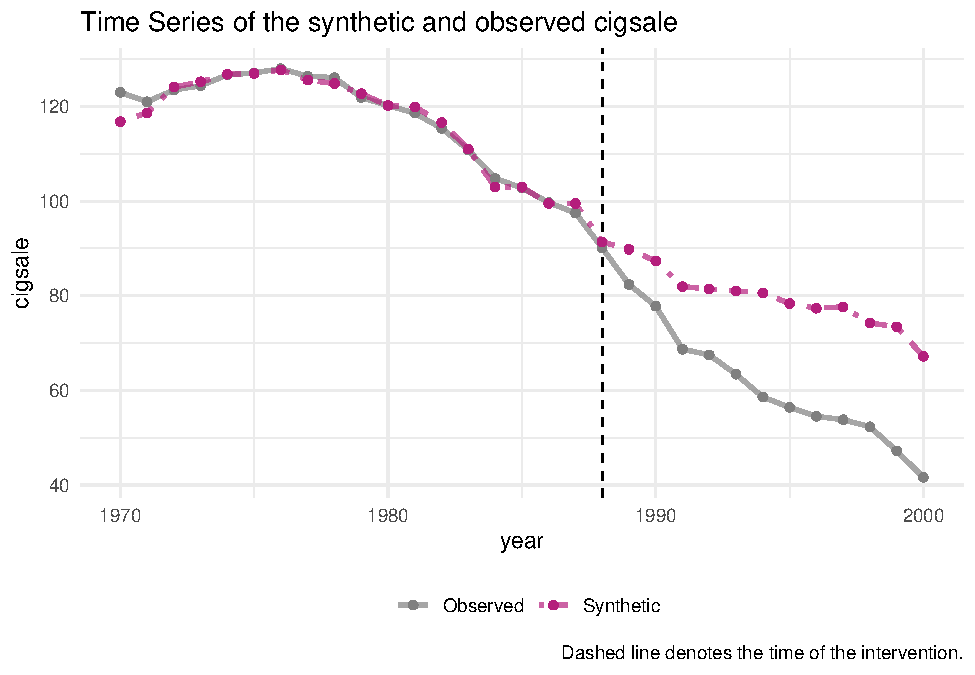
\includegraphics[keepaspectratio,alt={\label{fig:cigarro-tidysynth}Trajetória observada da Califórnia e controle sintético estimado pelo pacote tidysynth.}]{bookdownproj_files/figure-latex/cigarro-tidysynth-1.pdf}}
\caption{\label{fig:cigarro-tidysynth}Trajetória observada da Califórnia e controle sintético estimado pelo pacote tidysynth.}
\end{figure}

O gráfico mostra que a Califórnia Sintética acompanha bem a trajetória real no período pré-1988, e diverge no período pós --- essa divergência é a estimativa do efeito causal.

A quantidade causal de interesse --- a diferença entre observado e sintético --- pode ser visualizada diretamente:

\begin{Shaded}
\begin{Highlighting}[]
\NormalTok{smoking\_out }\SpecialCharTok{\%\textgreater{}\%} \FunctionTok{plot\_differences}\NormalTok{()}
\end{Highlighting}
\end{Shaded}

\begin{figure}
\centering
\pandocbounded{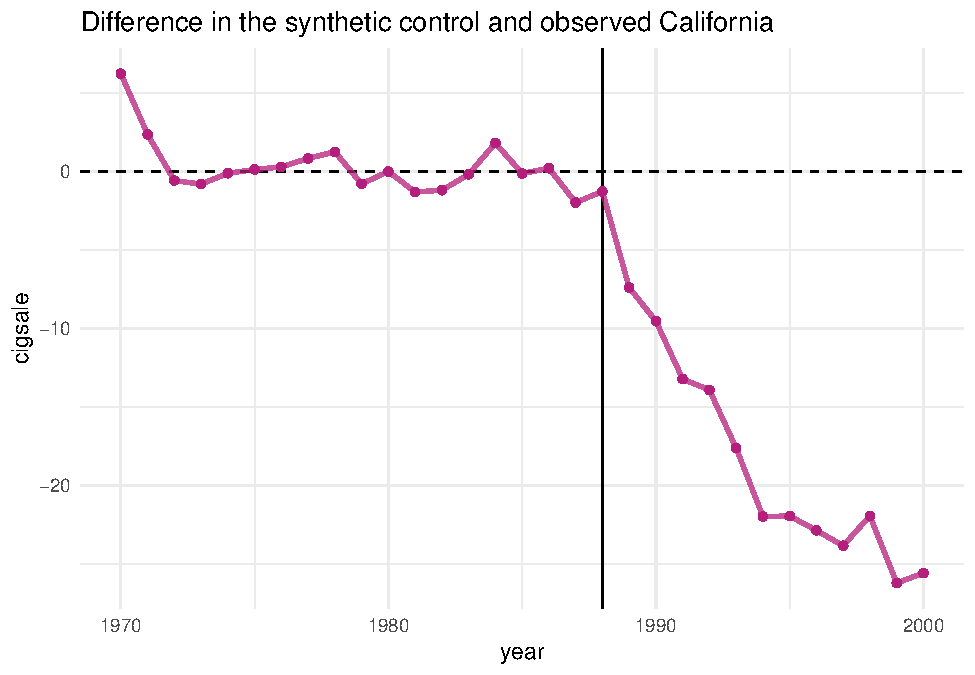
\includegraphics[keepaspectratio,alt={\label{fig:cigarro-tidysynth-diferencas}Diferença entre Califórnia observada e controle sintético ao longo do tempo.}]{bookdownproj_files/figure-latex/cigarro-tidysynth-diferencas-1.pdf}}
\caption{\label{fig:cigarro-tidysynth-diferencas}Diferença entre Califórnia observada e controle sintético ao longo do tempo.}
\end{figure}

Os pesos atribuídos a cada estado e a cada variável preditora:

\begin{Shaded}
\begin{Highlighting}[]
\NormalTok{smoking\_out }\SpecialCharTok{\%\textgreater{}\%} \FunctionTok{plot\_weights}\NormalTok{()}
\end{Highlighting}
\end{Shaded}

\begin{figure}
\centering
\pandocbounded{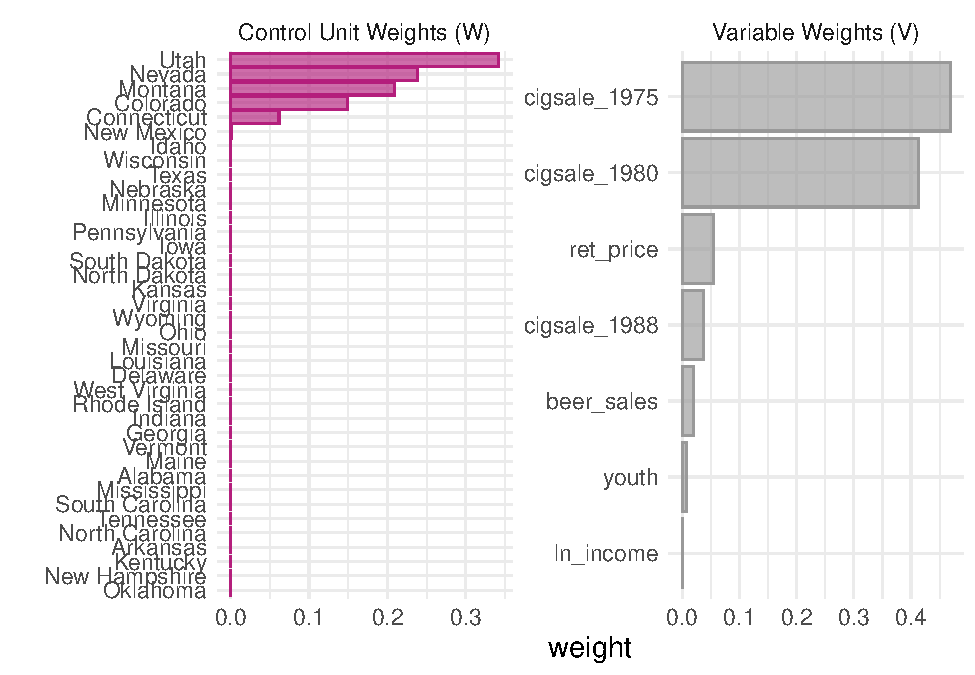
\includegraphics[keepaspectratio,alt={\label{fig:cigarro-tidysynth-pesos}Pesos atribuídos aos estados doadores e aos preditores no SCM estimado pelo pacote tidysynth.}]{bookdownproj_files/figure-latex/cigarro-tidysynth-pesos-1.pdf}}
\caption{\label{fig:cigarro-tidysynth-pesos}Pesos atribuídos aos estados doadores e aos preditores no SCM estimado pelo pacote tidysynth.}
\end{figure}

O balanceamento entre a Califórnia real e a sintética nos preditores:

\begin{Shaded}
\begin{Highlighting}[]
\NormalTok{smoking\_out }\SpecialCharTok{\%\textgreater{}\%}
  \FunctionTok{grab\_balance\_table}\NormalTok{() }\SpecialCharTok{\%\textgreater{}\%}
  \FunctionTok{kable}\NormalTok{(}\AttributeTok{caption =} \StringTok{"Balanceamento entre Califórnia observada e controle sintético nos preditores."}\NormalTok{)}
\end{Highlighting}
\end{Shaded}

\begin{table}

\caption{\label{tab:cigarro-tidysynth-balanceamento}Balanceamento entre Califórnia observada e controle sintético nos preditores.}
\centering
\begin{tabular}[t]{l|r|r|r}
\hline
variable & California & synthetic\_California & donor\_sample\\
\hline
ln\_income & 10.0765586 & 9.8534864 & 9.8291968\\
\hline
ret\_price & 89.4222234 & 89.3908482 & 87.2660819\\
\hline
youth & 0.1735324 & 0.1736054 & 0.1725101\\
\hline
beer\_sales & 24.2800003 & 24.2224860 & 23.6552632\\
\hline
cigsale\_1975 & 127.0999985 & 126.9914177 & 136.9315790\\
\hline
cigsale\_1980 & 120.1999969 & 120.2204841 & 138.0894737\\
\hline
cigsale\_1988 & 90.0999985 & 91.3888620 & 113.8236837\\
\hline
\end{tabular}
\end{table}

\subsubsection{Inferência por placebo}\label{inferuxeancia-por-placebo}

A inferência no SCM é feita por testes placebo. A intuição é a de um teste de permutação: para cada estado do donor pool, fingimos que ele foi tratado e estimamos um SCM. Se o efeito da Califórnia for grande relativo aos placebos, concluímos que é estatisticamente significativo.

\begin{Shaded}
\begin{Highlighting}[]
\NormalTok{smoking\_out }\SpecialCharTok{\%\textgreater{}\%} \FunctionTok{plot\_placebos}\NormalTok{()}
\end{Highlighting}
\end{Shaded}

\begin{figure}
\centering
\pandocbounded{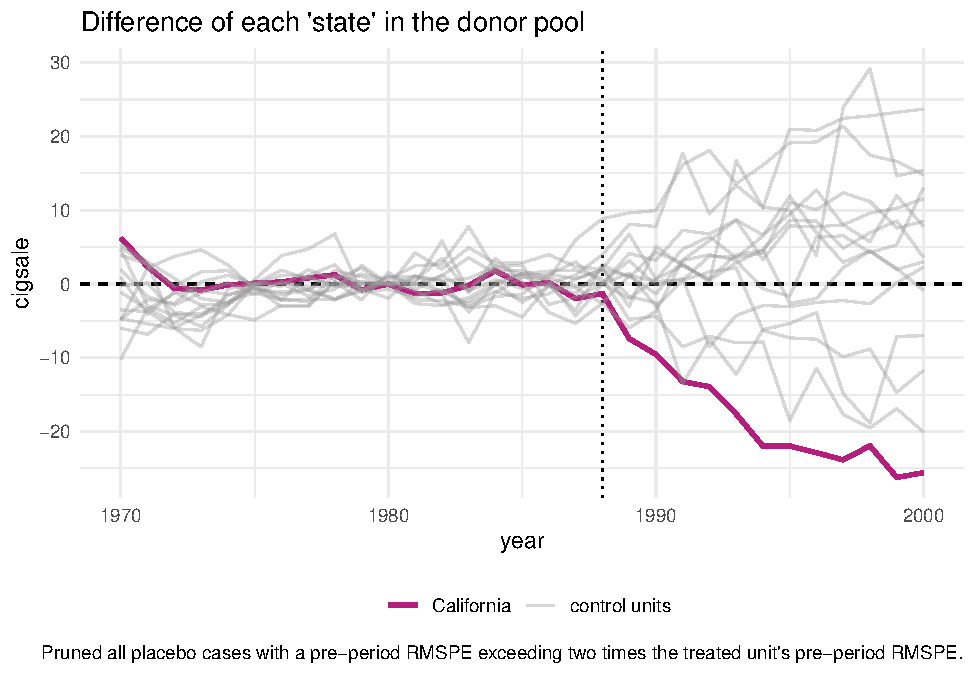
\includegraphics[keepaspectratio,alt={\label{fig:cigarro-tidysynth-placebos}Teste placebo do SCM para a Califórnia e os estados doadores.}]{bookdownproj_files/figure-latex/cigarro-tidysynth-placebos-1.pdf}}
\caption{\label{fig:cigarro-tidysynth-placebos}Teste placebo do SCM para a Califórnia e os estados doadores.}
\end{figure}

O efeito estimado para a Califórnia (linha escura) é claramente maior do que os efeitos placebo (linhas cinzas), sugerindo que a Proposição 99 de fato reduziu o consumo de cigarros.

Para formalizar a inferência, Abadie, Diamond e Hainmueller (2010, seção 4) propõem construir p-valores a partir da distribuição de razões de RMSPE: para cada unidade placebo \(i\), calcula-se a razão entre o RMSPE pós-tratamento e o RMSPE pré-tratamento. Se a razão da unidade tratada for extrema em relação à distribuição dos placebos, o efeito é considerado significativo. Formalmente, seja \(\mathcal{P}\) o conjunto de unidades usadas no teste placebo, incluindo a unidade tratada e as unidades doadoras elegíveis. O p-valor é a fração de unidades em \(\mathcal{P}\) cuja razão RMSPE é pelo menos tão grande quanto a da unidade tratada:

\[
\text{p-valor} = \frac{1}{N} \sum_{i \in \mathcal{P}} \mathbf{1}[R_i \geq R_{\text{tratada}}]
\]

onde \(N = |\mathcal{P}|\) e

\[
R_i =
\frac{
\sqrt{\frac{1}{T - T_0}\sum_{t > T_0} (Y_{it} - \hat{Y}_{it}(0))^2}
}{
\sqrt{\frac{1}{T_0}\sum_{t \leq T_0} (Y_{it} - \hat{Y}_{it}(0))^2}
}
\]

é a razão entre o RMSPE pós-tratamento e o RMSPE pré-tratamento da unidade \(i\).

\textbf{Limitação fundamental: o que significam ``5\%''?} É crucial entender o que esse p-valor realmente mede. Sob a hipótese nula de efeito zero, o teste assume que a unidade tratada ``não é diferente'' das demais. O p-valor de 5\% significa que, \emph{se cada uma das \(N\) unidades fosse tratada}, 5\% delas teriam o null rejeitado. Mas isso \textbf{não é um nível de significância no sentido frequentista convencional}, porque a unidade tratada geralmente não foi escolhida aleatoriamente entre as \(N\) unidades. A Califórnia aprovou a Proposição 99 por razões políticas e sociais específicas --- não foi sorteada. Se a Califórnia é sistematicamente diferente dos outros estados (o que é provável, dado que \emph{ela} adotou a política), o teste de permutação pode ter propriedades de tamanho distorcidas.

Em outras palavras, o teste tem validade exata sob aleatorização do tratamento, mas essa premissa raramente se sustenta em aplicações de controle sintético. Abadie, Diamond e Hainmueller (2015), ao estudar o impacto da reunificação sobre a Alemanha Ocidental, enfrentam esse problema de forma aguda: o que significaria ``atribuir a reunificação a outro país''?

\textbf{Complicações adicionais na prática.} Mesmo aceitando a lógica do teste, duas complicações surgem. Primeira: para algumas unidades placebo, o controle sintético pode ter ajuste pré-tratamento ruim. Isso contamina especialmente estatísticas baseadas apenas no erro pós-tratamento em nível; por isso, a razão RMSPE pós/pré é preferível, e também é comum descartar placebos com RMSPE pré-tratamento acima de um limiar. Segunda: com poucas unidades elegíveis no exercício placebo (\(N\) pequeno), o menor p-valor possível é \(1/N\). No exemplo da Califórnia, \(N = 39\) porque a amostra contém a Califórnia e 38 estados doadores, não todos os estados dos EUA; portanto, o menor p-valor é \(1/39 \approx 0.026\), o que limita a precisão inferencial.

\textbf{Inferência conformal como alternativa.} Chernozhukov, Wüthrich e Zhu (2021) propõem uma solução elegante: em vez de permutar \emph{unidades}, permutar \emph{períodos de tempo}. A ideia é que, sob a hipótese nula de efeito zero, os resíduos \(Y_{N,t} - \hat{Y}_{N,t}(0)\) nos períodos pós-tratamento deveriam ser indistinguíveis dos resíduos pré-tratamento. O teste conformal constrói p-valores permutando esses resíduos ao longo do tempo --- sem necessidade de assumir que o tratamento foi atribuído aleatoriamente entre unidades. Isso fornece inferência com validade em amostra finita, mesmo com uma única unidade tratada, desde que os erros sejam permutáveis ao longo do tempo.

\subsubsection{Diagnósticos de robustez do SCM}\label{diagnuxf3sticos-de-robustez-do-scm}

Além dos testes placebo, dois diagnósticos adicionais são recomendados para avaliar a robustez do SCM (Abadie, 2021):

\textbf{Teste de backdating.} O pesquisador finge que o tratamento ocorreu em um período anterior ao verdadeiro --- por exemplo, 5 ou 10 anos antes --- e reestima o SCM. Se o controle sintético divergir da unidade tratada \emph{antes} do verdadeiro tratamento, isso sugere que o modelo não está capturando adequadamente a dinâmica pré-tratamento e que as estimativas pós-tratamento podem ser enviesadas. Abadie (2021) ilustra essa abordagem no caso da reunificação alemã, mostrando que a Alemanha Ocidental Sintética acompanha de perto o PIB real até 1990.

\textbf{Teste leave-one-out.} Remove-se cada doador contribuinte (com peso não-zero) do donor pool, um de cada vez, e reestima-se o SCM. Se as estimativas são robustas --- isto é, se o efeito estimado não muda substancialmente ao remover qualquer doador individual --- há maior confiança de que o resultado não depende de uma única unidade de controle. Se, ao contrário, a remoção de um doador altera dramaticamente as estimativas, isso indica fragilidade.

\textbf{Sensibilidade ao donor pool.} Mais geralmente, os resultados do SCM podem ser sensíveis à composição do donor pool. O pesquisador deve justificar os critérios de inclusão e exclusão de unidades de controle com base em conhecimento substantivo --- por exemplo, excluindo estados com políticas antitabaco similares ou com características estruturais muito diferentes (Abadie, 2021). Recomenda-se verificar a robustez das estimativas a variações na composição do donor pool.

\subsection{Do SCM aos modelos de fatores}\label{do-scm-aos-modelos-de-fatores}

Como vimos na seção anterior, o SCM é justificado por um modelo linear de fatores: \(Y_{it}(0) = \delta_t + \theta_t Z_i + \lambda_t \mu_i + \varepsilon_{it}\). Se os pesos reproduzem os preditores pré-tratamento, eles também reproduzem os fatores latentes, e o viés desaparece. Mas isso levanta uma questão natural: \textbf{se o processo gerador de dados é um modelo de fatores, por que não estimar os fatores diretamente?}

No caso clássico do SCM --- uma única unidade tratada, poucas unidades de controle --- a resposta é pragmática: com \(N\) pequeno, não há graus de liberdade suficientes para estimar fatores latentes de forma confiável. O SCM contorna essa limitação impondo convexidade, que regulariza o problema. Mas quando temos \textbf{múltiplas unidades tratadas} (possivelmente com tratamento escalonado no tempo) e um painel razoavelmente grande, podemos estimar o modelo de fatores diretamente --- e potencialmente obter estimativas mais eficientes.

Essa é a motivação para os métodos que apresentamos a seguir: o framework de estimação contrafactual de Liu, Wang e Xu (2024) e o Synthetic DiD de Arkhangelsky et al.~(2021). Ambos exploram a estrutura de fatores de formas diferentes --- o primeiro estimando os fatores diretamente, o segundo usando pesos que são robustos à presença de fatores --- mas compartilham a mesma lógica de imputar \(Y_{it}(0)\).

\subsection{Framework de estimação contrafactual}\label{framework-de-estimauxe7uxe3o-contrafactual}

O SCM clássico é uma ferramenta poderosa para estudos de caso com uma única unidade tratada. Mas e quando temos múltiplas unidades tratadas com tratamento escalonado no tempo? E quando queremos diagnósticos formais sobre a qualidade da estimação?

Liu, Wang e Xu (2024) propõem um framework unificado de \textbf{estimação contrafactual} que generaliza o SCM e o DiD por imputação (para um survey mais amplo de modelos causais para dados de painel, ver Arkhangelsky e Imbens, 2024). A ideia central é a mesma: estimar \(Y_{it}(0)\) para as observações tratadas e calcular o efeito como a diferença entre observado e contrafactual.

\subsubsection{Setup}\label{setup}

Considere um painel com \(N\) unidades e \(T\) períodos. O indicador de tratamento \(D_{it}\) pode variar por unidade e tempo (tratamento escalonado, e inclusive pode ``ligar e desligar''). Particione as observações em dois conjuntos:

\begin{itemize}
\tightlist
\item
  \(\mathcal{C}_0\): observações não-tratadas (\(D_{it} = 0\)), usadas para estimar o modelo
\item
  \(\mathcal{M}\): observações tratadas (\(D_{it} = 1\)), para as quais imputamos o contrafactual
\end{itemize}

O efeito individual do tratamento é \(\delta_{it} = Y_{it}(1) - Y_{it}(0)\), e o estimando é:
\[
ATT = \mathbb{E}[\delta_{it} \mid D_{it} = 1] = \frac{1}{|\mathcal{M}|} \sum_{(i,t) \in \mathcal{M}} \delta_{it}
\]

A segunda igualdade vale sob uma interpretação \emph{design-based}, em que o painel observado é a população de interesse (não uma amostra de uma superpopulação). Nesse caso, a expectativa é sobre a atribuição de tratamento, e a média amostral coincide com o parâmetro populacional.

\subsubsection{Estratégia de estimação em quatro passos}\label{estratuxe9gia-de-estimauxe7uxe3o-em-quatro-passos}

\begin{enumerate}
\def\labelenumi{\arabic{enumi}.}
\tightlist
\item
  \textbf{Ajustar} o modelo de \(Y_{it}(0)\) usando apenas as observações em \(\mathcal{C}_0\)
\item
  \textbf{Prever} o contrafactual \(\hat{Y}_{it}(0)\) para cada \((i,t) \in \mathcal{M}\)
\item
  \textbf{Calcular} \(\hat{\delta}_{it} = Y_{it} - \hat{Y}_{it}(0)\) para cada observação tratada
\item
  \textbf{Agregar} os efeitos: \(\widehat{ATT} = \frac{1}{|\mathcal{M}|} \sum_{(i,t) \in \mathcal{M}} \hat{\delta}_{it}\)
\end{enumerate}

Essa estratégia evita o problema de pesos negativos do TWFE (capítulo 8): cada observação tratada recebe peso uniforme \(1/|\mathcal{M}|\) na agregação.

\subsubsection{Suposições de identificação}\label{suposiuxe7uxf5es-de-identificauxe7uxe3o-1}

O framework requer três suposições (Liu et al., 2024, p.~163):

\begin{itemize}
\tightlist
\item
  \textbf{Suposição 1 (Forma funcional)}: \(Y_{it}(0) = h(U_{it}) + \varepsilon_{it}\), onde \(h\) é uma função desconhecida e \(U_{it}\) são fatores latentes.
\item
  \textbf{Suposição 2 (Exogeneidade estrita)}: \(\mathbb{E}[\varepsilon_{it} | U_{i1}, \ldots, U_{iT}, D_{i1}, \ldots, D_{iT}] = 0\) --- os erros são não-correlacionados com os fatores e o tratamento.
\item
  \textbf{Suposição 3 (Decomposição de baixo posto)}: \(h(U_{it})\) pode ser decomposta em componentes de baixa dimensionalidade.
\end{itemize}

A Suposição 3 é o que diferencia os três estimadores: no caso mais simples, \(h(U_{it}) = \alpha_i + \xi_t\) (efeitos fixos aditivos, como no DiD). No caso mais flexível, \(h(U_{it}) = \alpha_i + \xi_t + \lambda'_i f_t\) (fatores interativos).

\subsubsection{Conexão com DiD}\label{conexuxe3o-com-did}

O DiD é um caso especial deste framework. Quando \(h(U_{it}) = \alpha_i + \xi_t\) e usamos os dados de controle para estimar esses efeitos fixos e depois imputamos, obtemos o estimador de DiD por imputação de Borusyak, Jaravel e Spiess (2024), que vimos no capítulo 8. O framework de Liu et al.~vai além ao permitir modelos mais flexíveis.

\subsection{Três estimadores contrafactuais}\label{truxeas-estimadores-contrafactuais}

O framework de Liu et al.~(2024) oferece três estimadores, implementados no pacote \texttt{fect} (Fixed Effects Counterfactual Estimators).

\subsubsection{FEct: efeitos fixos}\label{fect-efeitos-fixos}

O modelo mais simples assume:
\[
Y_{it}(0) = X'_{it}\beta + \alpha_i + \xi_t + \varepsilon_{it}
\]

Esse é o modelo TWFE --- os mesmos efeitos fixos aditivos do DiD. A diferença em relação ao DiD tradicional é a \emph{estratégia de estimação}: em vez de regredir \(Y\) em \(D\) com efeitos fixos (o que pode gerar pesos negativos com tratamento heterogêneo), o FEct estima \(\alpha_i\), \(\xi_t\) e \(\beta\) usando apenas as observações não-tratadas, e depois imputa o contrafactual para as tratadas.

Isso é equivalente ao estimador de imputação de Borusyak et al.~(2024), que discutimos no capítulo 8.

\textbf{Nota sobre covariáveis.} O termo \(X'_{it}\beta\) permite incluir covariáveis no modelo. As mesmas precauções discutidas no capítulo 8 (seção sobre DiD com covariáveis) se aplicam: covariáveis variantes no tempo que podem ser afetadas pelo tratamento são \emph{bad controls} e não devem ser incluídas diretamente. A vantagem da abordagem de imputação (FEct/IFEct) é que \(\beta\) é estimado usando apenas observações não-tratadas, evitando a contaminação que ocorre no TWFE ingênuo.

\subsubsection{IFEct: fatores interativos}\label{ifect-fatores-interativos}

O modelo de fatores interativos adiciona um componente multiplicativo:
\[
Y_{it}(0) = X'_{it}\beta + \alpha_i + \xi_t + \lambda'_i f_t + \varepsilon_{it}
\]

O termo \(\lambda'_i f_t\) captura confundidores variantes no tempo de forma heterogênea: \(f_t\) é um vetor de \(r\) fatores comuns (que variam no tempo), e \(\lambda_i\) é o vetor de cargas fatoriais (que variam por unidade). Quando \(f_t\) é constante, o componente \(\lambda'_i f_t\) é absorvido pelo efeito fixo de unidade \(\alpha_i\), e o modelo reduz ao caso aditivo (FEct); quando \(\lambda_i\) é constante, o componente é absorvido pelo efeito fixo de tempo \(\xi_t\).

A vantagem em relação ao FEct é que o IFEct \textbf{relaxa a suposição de tendências paralelas}: não exige que todas as unidades sigam a mesma tendência temporal. Basta que as trajetórias sejam explicáveis por um número pequeno de fatores latentes --- uma suposição mais fraca e frequentemente mais realista.

O número de fatores \(r\) é escolhido por validação cruzada. Na prática, o pacote \texttt{fect} testa \(r = 0, 1, 2, \ldots, r_{max}\) e escolhe o valor que minimiza o erro de predição nos dados não-tratados.

\subsubsection{MC: Matrix Completion}\label{mc-matrix-completion}

O estimador MC (Athey, Bayati, Doudchenko, Imbens e Khosravi, 2021) trata o problema como \emph{completação de matriz}. A ideia é que a matriz \(\mathbf{Y}(0)\) de resultados potenciais sem tratamento tem estrutura de baixo posto --- pode ser bem aproximada por uma matriz de posto \(r\) pequeno. O modelo é:
\[
\mathbf{Y}(0) = \mathbf{X}\beta + \mathbf{L} + \varepsilon
\]
onde \(\mathbf{L}\) é uma matriz de baixo posto. Em vez de selecionar \(r\) fatores diretamente (como no IFEct), o MC penaliza a norma nuclear \(\|\mathbf{L}\|_*\), que é uma relaxação convexa do posto. Isso faz um ``soft impute'': os valores singulares são encolhidos continuamente, em vez de truncados.

A diferença prática entre IFEct e MC é:

\begin{itemize}
\tightlist
\item
  \textbf{IFEct} faz ``hard impute'': escolhe \(r\) fatores e descarta o resto
\item
  \textbf{MC} faz ``soft impute'': penaliza a norma nuclear, encolhendo todos os valores singulares
\end{itemize}

Quando a penalização \(\lambda_L \to \infty\) (ou \(r = 0\)), ambos reduzem ao FEct (efeitos fixos aditivos).

\subsubsection{Demonstração com dados da Califórnia}\label{demonstrauxe7uxe3o-com-dados-da-califuxf3rnia}

Aplicamos os três estimadores aos mesmos dados de cigarros usados no SCM.

\begin{Shaded}
\begin{Highlighting}[]
\FunctionTok{library}\NormalTok{(fect)}
\FunctionTok{library}\NormalTok{(tidyverse)}

\FunctionTok{data}\NormalTok{(smoking, }\AttributeTok{package =} \StringTok{"tidysynth"}\NormalTok{)}

\CommentTok{\# Preparar dados para fect}
\NormalTok{df\_fect }\OtherTok{\textless{}{-}}\NormalTok{ smoking }\SpecialCharTok{\%\textgreater{}\%}
  \FunctionTok{mutate}\NormalTok{(}
    \AttributeTok{D =} \FunctionTok{ifelse}\NormalTok{(state }\SpecialCharTok{==} \StringTok{"California"} \SpecialCharTok{\&}\NormalTok{ year }\SpecialCharTok{\textgreater{}=} \DecValTok{1989}\NormalTok{, }\DecValTok{1}\NormalTok{, }\DecValTok{0}\NormalTok{),}
    \AttributeTok{unit\_id =} \FunctionTok{as.numeric}\NormalTok{(}\FunctionTok{as.factor}\NormalTok{(state))}
\NormalTok{  )}

\CommentTok{\# FEct: efeitos fixos (equivalente a DiD por imputação)}
\NormalTok{out\_fe }\OtherTok{\textless{}{-}} \FunctionTok{fect}\NormalTok{(cigsale }\SpecialCharTok{\textasciitilde{}}\NormalTok{ D, }\AttributeTok{data =}\NormalTok{ df\_fect,}
               \AttributeTok{index =} \FunctionTok{c}\NormalTok{(}\StringTok{"state"}\NormalTok{, }\StringTok{"year"}\NormalTok{),}
               \AttributeTok{method =} \StringTok{"fe"}\NormalTok{,}
               \AttributeTok{se =} \ConstantTok{TRUE}\NormalTok{, }\AttributeTok{nboots =} \DecValTok{200}\NormalTok{,}
               \AttributeTok{parallel =} \ConstantTok{FALSE}\NormalTok{)}

\FunctionTok{cat}\NormalTok{(}\StringTok{"FEct {-} ATT estimado:"}\NormalTok{, }\FunctionTok{round}\NormalTok{(out\_fe}\SpecialCharTok{$}\NormalTok{att.avg, }\DecValTok{2}\NormalTok{), }\StringTok{"}\SpecialCharTok{\textbackslash{}n}\StringTok{"}\NormalTok{)}
\end{Highlighting}
\end{Shaded}

\begin{verbatim}
## FEct - ATT estimado: -27.35
\end{verbatim}

\begin{Shaded}
\begin{Highlighting}[]
\CommentTok{\# IFEct: fatores interativos (r escolhido por CV)}
\NormalTok{out\_ife }\OtherTok{\textless{}{-}} \FunctionTok{fect}\NormalTok{(cigsale }\SpecialCharTok{\textasciitilde{}}\NormalTok{ D, }\AttributeTok{data =}\NormalTok{ df\_fect,}
                \AttributeTok{index =} \FunctionTok{c}\NormalTok{(}\StringTok{"state"}\NormalTok{, }\StringTok{"year"}\NormalTok{),}
                \AttributeTok{method =} \StringTok{"ife"}\NormalTok{,}
                \AttributeTok{r =} \FunctionTok{c}\NormalTok{(}\DecValTok{0}\NormalTok{, }\DecValTok{5}\NormalTok{),}
                \AttributeTok{CV =} \ConstantTok{TRUE}\NormalTok{,}
                \AttributeTok{se =} \ConstantTok{TRUE}\NormalTok{, }\AttributeTok{nboots =} \DecValTok{200}\NormalTok{,}
                \AttributeTok{parallel =} \ConstantTok{FALSE}\NormalTok{)}

\FunctionTok{cat}\NormalTok{(}\StringTok{"IFEct {-} ATT estimado:"}\NormalTok{, }\FunctionTok{round}\NormalTok{(out\_ife}\SpecialCharTok{$}\NormalTok{att.avg, }\DecValTok{2}\NormalTok{), }\StringTok{"}\SpecialCharTok{\textbackslash{}n}\StringTok{"}\NormalTok{)}
\end{Highlighting}
\end{Shaded}

\begin{verbatim}
## IFEct - ATT estimado: -25.54
\end{verbatim}

\begin{Shaded}
\begin{Highlighting}[]
\FunctionTok{cat}\NormalTok{(}\StringTok{"Número de fatores escolhido:"}\NormalTok{, out\_ife}\SpecialCharTok{$}\NormalTok{r.cv, }\StringTok{"}\SpecialCharTok{\textbackslash{}n}\StringTok{"}\NormalTok{)}
\end{Highlighting}
\end{Shaded}

\begin{verbatim}
## Número de fatores escolhido: 4
\end{verbatim}

\begin{Shaded}
\begin{Highlighting}[]
\CommentTok{\# MC: Matrix Completion}
\NormalTok{out\_mc }\OtherTok{\textless{}{-}} \FunctionTok{fect}\NormalTok{(cigsale }\SpecialCharTok{\textasciitilde{}}\NormalTok{ D, }\AttributeTok{data =}\NormalTok{ df\_fect,}
               \AttributeTok{index =} \FunctionTok{c}\NormalTok{(}\StringTok{"state"}\NormalTok{, }\StringTok{"year"}\NormalTok{),}
               \AttributeTok{method =} \StringTok{"mc"}\NormalTok{,}
               \AttributeTok{se =} \ConstantTok{TRUE}\NormalTok{, }\AttributeTok{nboots =} \DecValTok{200}\NormalTok{,}
               \AttributeTok{parallel =} \ConstantTok{FALSE}\NormalTok{)}

\FunctionTok{cat}\NormalTok{(}\StringTok{"MC {-} ATT estimado:"}\NormalTok{, }\FunctionTok{round}\NormalTok{(out\_mc}\SpecialCharTok{$}\NormalTok{att.avg, }\DecValTok{2}\NormalTok{), }\StringTok{"}\SpecialCharTok{\textbackslash{}n}\StringTok{"}\NormalTok{)}
\end{Highlighting}
\end{Shaded}

\begin{verbatim}
## MC - ATT estimado: -25.91
\end{verbatim}

O gráfico de efeitos dinâmicos (\emph{dynamic treatment effects}) mostra a evolução do efeito estimado ao longo do tempo, incluindo o período pré-tratamento (que deve ser próximo de zero se o modelo estiver bem especificado):

\begin{Shaded}
\begin{Highlighting}[]
\FunctionTok{par}\NormalTok{(}\AttributeTok{mfrow =} \FunctionTok{c}\NormalTok{(}\DecValTok{1}\NormalTok{, }\DecValTok{3}\NormalTok{))}
\FunctionTok{plot}\NormalTok{(out\_fe, }\AttributeTok{main =} \StringTok{"FEct (Efeitos Fixos)"}\NormalTok{, }\AttributeTok{ylab =} \StringTok{"Efeito estimado"}\NormalTok{, }\AttributeTok{xlab =} \StringTok{"Períodos relativos ao tratamento"}\NormalTok{)}
\end{Highlighting}
\end{Shaded}

\begin{figure}
\centering
\pandocbounded{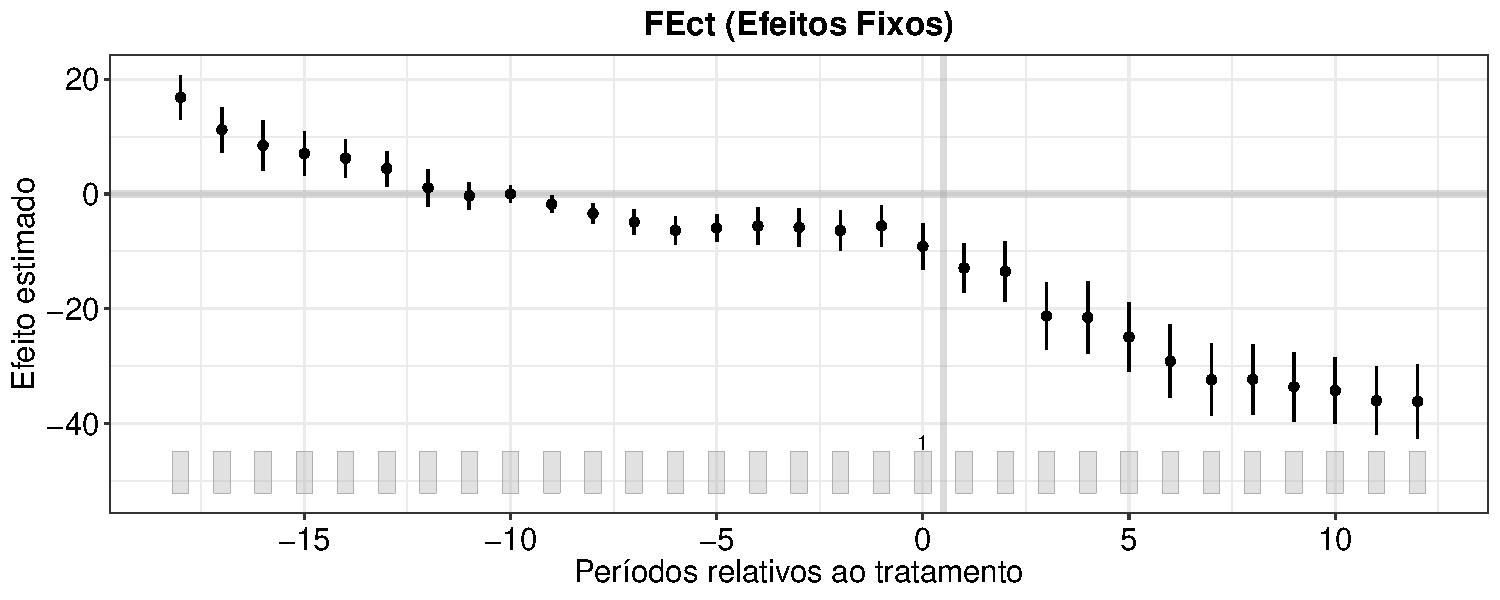
\includegraphics[keepaspectratio,alt={\label{fig:fect-dinamico-1}Efeitos dinâmicos estimados pelo FEct no exemplo da Califórnia.}]{bookdownproj_files/figure-latex/fect-dinamico-1.pdf}}
\caption{\label{fig:fect-dinamico-1}Efeitos dinâmicos estimados pelo FEct no exemplo da Califórnia.}
\end{figure}

\begin{Shaded}
\begin{Highlighting}[]
\FunctionTok{plot}\NormalTok{(out\_ife, }\AttributeTok{main =} \StringTok{"IFEct (Fatores Interativos)"}\NormalTok{, }\AttributeTok{ylab =} \StringTok{"Efeito estimado"}\NormalTok{, }\AttributeTok{xlab =} \StringTok{"Períodos relativos ao tratamento"}\NormalTok{)}
\end{Highlighting}
\end{Shaded}

\begin{figure}
\centering
\pandocbounded{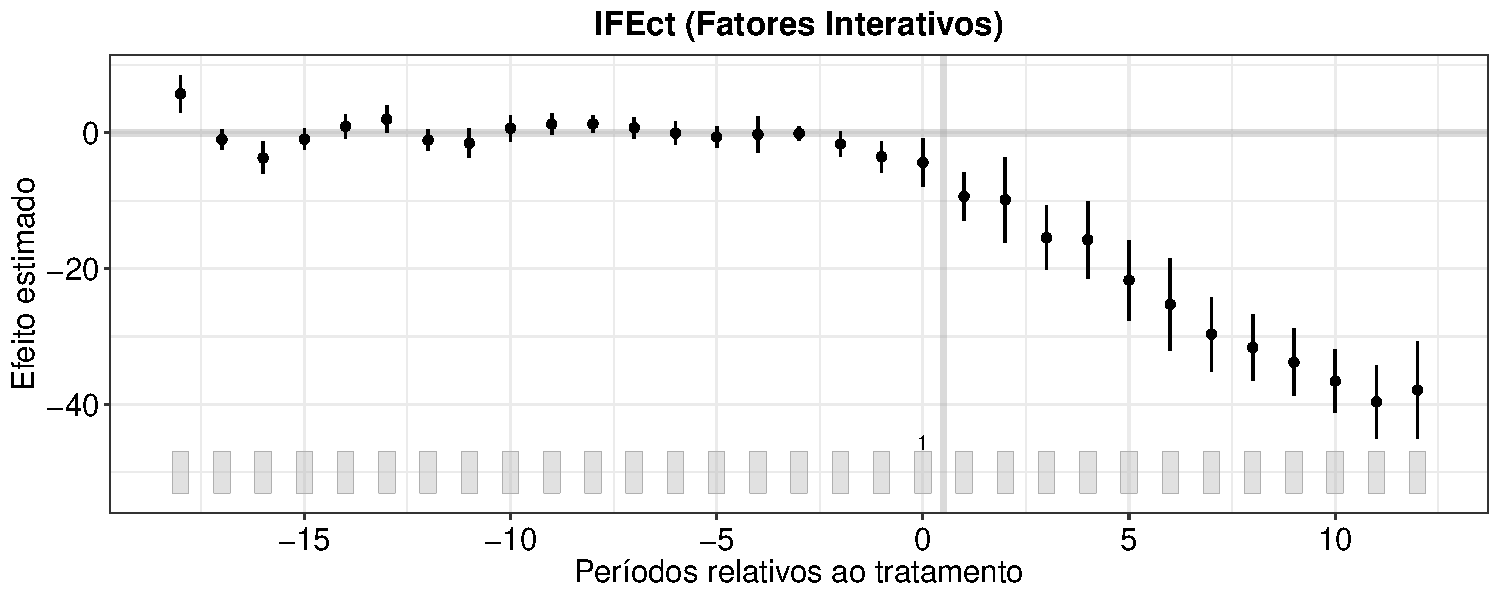
\includegraphics[keepaspectratio,alt={\label{fig:fect-dinamico-2}Efeitos dinâmicos estimados pelo IFEct no exemplo da Califórnia.}]{bookdownproj_files/figure-latex/fect-dinamico-2.pdf}}
\caption{\label{fig:fect-dinamico-2}Efeitos dinâmicos estimados pelo IFEct no exemplo da Califórnia.}
\end{figure}

\begin{Shaded}
\begin{Highlighting}[]
\FunctionTok{plot}\NormalTok{(out\_mc, }\AttributeTok{main =} \StringTok{"MC (Matrix Completion)"}\NormalTok{, }\AttributeTok{ylab =} \StringTok{"Efeito estimado"}\NormalTok{, }\AttributeTok{xlab =} \StringTok{"Períodos relativos ao tratamento"}\NormalTok{)}
\end{Highlighting}
\end{Shaded}

\begin{figure}
\centering
\pandocbounded{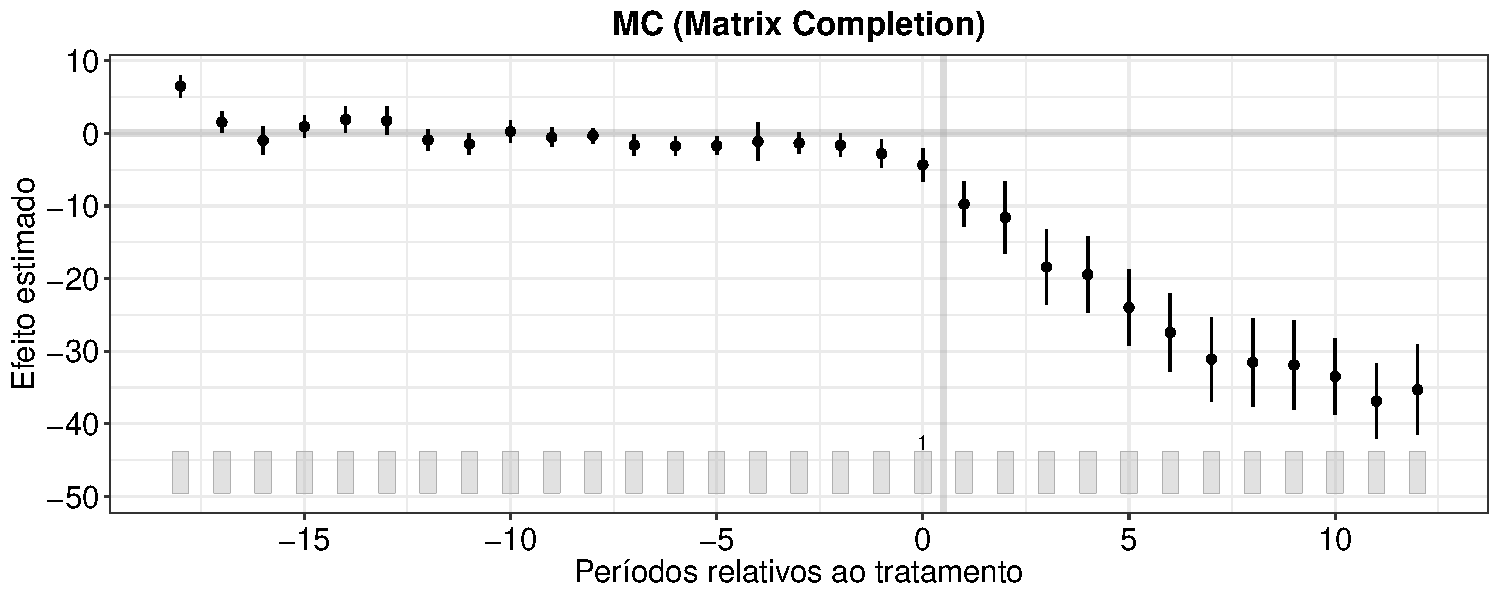
\includegraphics[keepaspectratio,alt={\label{fig:fect-dinamico-3}Efeitos dinâmicos estimados por matrix completion no exemplo da Califórnia.}]{bookdownproj_files/figure-latex/fect-dinamico-3.pdf}}
\caption{\label{fig:fect-dinamico-3}Efeitos dinâmicos estimados por matrix completion no exemplo da Califórnia.}
\end{figure}

Os três estimadores devem concordar no sinal e magnitude aproximada do efeito (redução nas vendas de cigarros). Divergências no período pré-tratamento indicam diferenças na qualidade do ajuste --- que é exatamente o que os diagnósticos formais da próxima seção avaliam.

\subsection{Diagnósticos}\label{diagnuxf3sticos}

Uma vantagem do framework de Liu et al.~(2024) é oferecer diagnósticos formais para avaliar a qualidade da estimação contrafactual. Esses diagnósticos vão além da inspeção visual e fornecem testes estatísticos.

\subsubsection{Efeitos dinâmicos}\label{efeitos-dinuxe2micos}

O gráfico de efeitos dinâmicos (\emph{gap plot}) mostra \(\hat{\delta}_{it}\) para cada período relativo ao tratamento. No período pré-tratamento, esses efeitos devem ser próximos de zero --- se não forem, o modelo está falhando em reproduzir os dados pré-tratamento e as estimativas pós-tratamento são suspeitas.

Diferentemente do event study tradicional do DiD (capítulo 8), o gráfico do \texttt{fect} não precisa de uma categoria de referência arbitrária: todos os períodos pré-tratamento são informativos.

\subsubsection{Placebo test}\label{placebo-test}

O teste placebo ``esconde'' parte dos períodos pré-tratamento e finge que o tratamento começou antes. Formalmente, remove os últimos \(L\) períodos pré-tratamento de \(\mathcal{C}_0\), reestima o modelo, e calcula \(\hat{\delta}_{it}\) para esses períodos ``escondidos''. Se o modelo for bem especificado, esses efeitos placebo devem ser zero.

Liu et al.~(2024) propõem dois critérios:

\begin{enumerate}
\def\labelenumi{\arabic{enumi}.}
\tightlist
\item
  \textbf{Teste t}: a média dos efeitos placebo é significativamente diferente de zero?
\item
  \textbf{Teste de equivalência (TOST)}: os efeitos placebo estão dentro de um intervalo de equivalência \([-\Delta, \Delta]\)?
\end{enumerate}

O teste de equivalência é preferível porque um teste t com baixo poder pode falhar em rejeitar (falso conforto), enquanto o TOST requer evidência \emph{positiva} de que os efeitos são pequenos.

\begin{Shaded}
\begin{Highlighting}[]
\CommentTok{\# Placebo test com IFEct (r fixo, sem CV)}
\NormalTok{out\_ife\_placebo }\OtherTok{\textless{}{-}} \FunctionTok{fect}\NormalTok{(cigsale }\SpecialCharTok{\textasciitilde{}}\NormalTok{ D, }\AttributeTok{data =}\NormalTok{ df\_fect,}
                        \AttributeTok{index =} \FunctionTok{c}\NormalTok{(}\StringTok{"state"}\NormalTok{, }\StringTok{"year"}\NormalTok{),}
                        \AttributeTok{method =} \StringTok{"ife"}\NormalTok{,}
                        \AttributeTok{r =} \DecValTok{2}\NormalTok{,}
                        \AttributeTok{se =} \ConstantTok{TRUE}\NormalTok{, }\AttributeTok{nboots =} \DecValTok{200}\NormalTok{,}
                        \AttributeTok{parallel =} \ConstantTok{FALSE}\NormalTok{,}
                        \AttributeTok{placeboTest =} \ConstantTok{TRUE}\NormalTok{,}
                        \AttributeTok{placebo.period =} \FunctionTok{c}\NormalTok{(}\SpecialCharTok{{-}}\DecValTok{2}\NormalTok{, }\DecValTok{0}\NormalTok{))}

\FunctionTok{plot}\NormalTok{(out\_ife\_placebo, }\AttributeTok{type =} \StringTok{"equiv"}\NormalTok{, }\AttributeTok{main =} \StringTok{"Teste de Equivalência (IFEct)"}\NormalTok{)}
\end{Highlighting}
\end{Shaded}

\begin{figure}
\centering
\pandocbounded{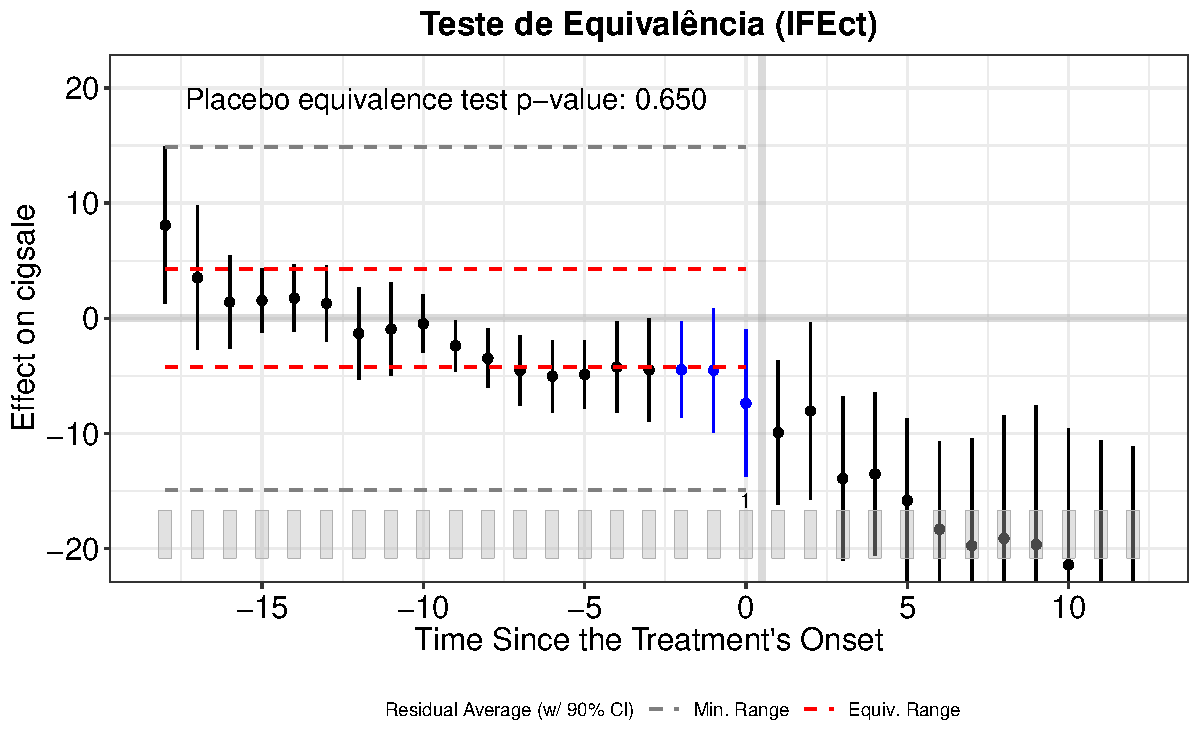
\includegraphics[keepaspectratio,alt={\label{fig:fect-placebo}Teste de equivalência placebo para o modelo IFEct no exemplo da Califórnia.}]{bookdownproj_files/figure-latex/fect-placebo-1.pdf}}
\caption{\label{fig:fect-placebo}Teste de equivalência placebo para o modelo IFEct no exemplo da Califórnia.}
\end{figure}

\subsubsection{Teste de no-carryover}\label{teste-de-no-carryover}

Em alguns contextos, o tratamento pode ter efeitos residuais: mesmo após o tratamento ser ``desligado'', a unidade ainda é afetada. O teste de carryover esconde períodos imediatamente após o tratamento ser removido (se aplicável) e verifica se existem efeitos residuais. Em contextos como o nosso (tratamento absorvente), esse teste não se aplica diretamente, mas é relevante para designs em que o tratamento liga e desliga.

\subsection{Synthetic DiD}\label{synthetic-did}

O Controle Sintético clássico e o framework de estimação contrafactual resolvem o problema de imputação de formas diferentes. Uma terceira abordagem, proposta por Arkhangelsky, Athey, Hirshberg, Imbens e Wager (2021), combina as ideias do SCM e do DiD em um único estimador: o \textbf{Synthetic DiD} (SDiD).

Para entender o SDiD, é útil ver os três estimadores --- SC, DiD e SDiD --- lado a lado, seguindo a formulação unificada de Arkhangelsky et al.~(2021) e a exposição de Arkhangelsky e Imbens (2024).

O \textbf{Controle Sintético} pode ser reescrito como um problema de mínimos quadrados ponderados:
\[
(\hat{\mu}, \hat{\gamma}, \hat{\tau}^{SC}) = \arg\min_{\mu, \gamma, \tau}\ \sum_i \sum_t (y_{it} - \mu - \gamma_t - D_{it}\tau)^2 \hat{w}_i
\]
Note que não há efeitos fixos de unidade (\(\alpha_i\)) --- os pesos \(\hat{w}_i\) ``fazem o trabalho'' de tornar os controles comparáveis.

O \textbf{DiD} (via TWFE) inclui efeitos fixos mas dá peso igual a todas as unidades:
\[
(\hat{\mu}, \hat{\alpha}, \hat{\gamma}, \hat{\tau}^{DiD}) = \arg\min_{\mu, \alpha, \gamma, \tau}\ \sum_i \sum_t (y_{it} - \mu - \alpha_i - \gamma_t - D_{it}\tau)^2
\]

O \textbf{SDiD} combina ambos --- efeitos fixos \emph{e} pesos, tanto para unidades quanto para períodos:
\[
(\hat{\mu}, \hat{\alpha}, \hat{\gamma}, \hat{\tau}^{SDiD}) = \arg\min_{\mu, \alpha, \gamma, \tau}\ \sum_i \sum_t (y_{it} - \mu - \alpha_i - \gamma_t - D_{it}\tau)^2 \hat{w}_i \hat{\lambda}_t
\]

Os pesos de unidade \(\hat{w}_i\) balanceiam as tendências pré-tratamento: dão mais peso a unidades de controle cuja trajetória é similar à dos tratados. Os pesos temporais \(\hat{\lambda}_t\) balanceiam os períodos: dão mais peso a períodos pré-tratamento cuja estrutura de cross-section é similar ao período pós. Em outras palavras, os pesos reponderam as observações de modo a reduzir o viés sob um modelo de fatores latentes, mesmo quando tendências paralelas globais não são válidas. Arkhangelsky et al.~(2021) demonstram a consistência do SDiD sob um modelo de fatores quando as estimativas de pesos convergem adequadamente.

\textbf{O SDiD relaxa a suposição de tendências paralelas?} A resposta exige uma distinção cuidadosa. O modelo que o SDiD \emph{estima} é aditivo --- \(\alpha_i + \gamma_t\) --- o mesmo do DiD. Nesse sentido, o SDiD não modela fatores interativos como o IFEct. Mas Arkhangelsky et al.~(2021) demonstram que o SDiD é \textbf{consistente sob um modelo de fatores latentes} \(Y_{it}(0) = \alpha_i + \lambda'_i f_t + \varepsilon_{it}\) --- um DGP em que tendências paralelas globais \emph{não} valem. Como isso é possível?

A chave está nos pesos. Os pesos de unidade \(\hat{w}_i\) são construídos para que a média ponderada dos controles tenha a \emph{mesma tendência pré-tratamento} que os tratados. Os pesos temporais \(\hat{\lambda}_t\) são construídos para que a média ponderada dos períodos pré-tratamento tenha a \emph{mesma estrutura cross-section} que o período pós. Em conjunto, os pesos criam uma ``vizinhança'' local --- um subconjunto reponderado de unidades e períodos --- dentro da qual tendências paralelas valem aproximadamente, mesmo que não valham globalmente.

\textbf{Um exemplo concreto.} Suponha três estados de controle: A (tendência crescente), B (tendência estável) e C (tendência decrescente). Se o estado tratado tem tendência estável no pré-tratamento, o DiD daria peso \(1/3\) a cada controle e falharia (a média dos três não reproduz a tendência estável). O SDiD atribuiria peso alto a B (tendência similar) e pesos baixos a A e C --- criando localmente uma comparação com tendências paralelas.

\textbf{Qual é o limite dessa tolerância?} A consistência do SDiD sob o modelo de fatores depende de condições técnicas sobre a convergência dos pesos estimados (Arkhangelsky et al., 2021, Teorema 1). Na prática, isso requer que: (i) exista uma combinação convexa dos controles que reproduza a tendência dos tratados (ou seja, os tratados estejam no ``envoltório convexo'' dos controles em termos de cargas fatoriais \(\lambda_i\)); e (ii) haja períodos pré-tratamento suficientes para estimar os pesos com precisão. Se a unidade tratada tem cargas fatoriais muito diferentes de \emph{todos} os controles --- por exemplo, se a Califórnia tem uma dinâmica única que nenhuma combinação de outros estados consegue reproduzir --- os pesos não convergem e o SDiD não resolve o problema. Nesse cenário, seria necessário um estimador que modele os fatores diretamente, como o IFEct.

Em resumo: o SDiD não \emph{modela} tendências não-paralelas (como o IFEct), mas \emph{tolera} tendências não-paralelas via reponderação --- desde que a heterogeneidade das tendências possa ser eliminada por uma recomposição convexa das unidades de controle. É mais robusto que o DiD, mas não tão flexível quanto o IFEct em cenários com estrutura fatorial complexa.

\subsubsection{Implementação no R}\label{implementauxe7uxe3o-no-r}

Vamos aplicar DiD, SC e SDiD aos dados da Califórnia.

\begin{Shaded}
\begin{Highlighting}[]
\FunctionTok{library}\NormalTok{(fixest)}

\NormalTok{smoking\_did }\OtherTok{\textless{}{-}}\NormalTok{ smoking }\SpecialCharTok{\%\textgreater{}\%}
  \FunctionTok{mutate}\NormalTok{(}\AttributeTok{treatment =} \FunctionTok{ifelse}\NormalTok{(state }\SpecialCharTok{==} \StringTok{"California"} \SpecialCharTok{\&}\NormalTok{ year }\SpecialCharTok{\textgreater{}} \DecValTok{1988}\NormalTok{, }\DecValTok{1}\NormalTok{, }\DecValTok{0}\NormalTok{))}
\NormalTok{did }\OtherTok{\textless{}{-}} \FunctionTok{feols}\NormalTok{(cigsale }\SpecialCharTok{\textasciitilde{}}\NormalTok{ treatment }\SpecialCharTok{|}\NormalTok{ state }\SpecialCharTok{+}\NormalTok{ year, }\AttributeTok{data =}\NormalTok{ smoking\_did)}

\FunctionTok{summary}\NormalTok{(did)}
\end{Highlighting}
\end{Shaded}

\begin{verbatim}
## OLS estimation, Dep. Var.: cigsale
## Observations: 1,209
## Fixed-effects: state: 39,  year: 31
## Standard-errors: Clustered (state) 
##           Estimate Std. Error  t value           Pr(>|t|)    
## treatment -27.3491    2.80238 -9.75925 0.0000000000066913 ***
## ---
## Signif. codes:  0 '***' 0.001 '**' 0.01 '*' 0.05 '.' 0.1 ' ' 1
## RMSE: 11.5     Adj. R2: 0.870229
##              Within R2: 0.032671
\end{verbatim}

O estimador de DiD assume tendências paralelas na média --- suposição que pode não ser crível neste contexto, como mostra o event study:

\begin{Shaded}
\begin{Highlighting}[]
\FunctionTok{library}\NormalTok{(did2s)}
\FunctionTok{library}\NormalTok{(ggfixest)}

\NormalTok{df }\OtherTok{\textless{}{-}}\NormalTok{ smoking\_did }\SpecialCharTok{\%\textgreater{}\%}
  \FunctionTok{mutate}\NormalTok{(}\AttributeTok{event\_time =}\NormalTok{ year }\SpecialCharTok{{-}} \DecValTok{1988}\NormalTok{,}
         \AttributeTok{id =} \FunctionTok{as.integer}\NormalTok{(}\FunctionTok{as.factor}\NormalTok{(state))) }\SpecialCharTok{\%\textgreater{}\%}
  \FunctionTok{group\_by}\NormalTok{(state) }\SpecialCharTok{\%\textgreater{}\%}
  \FunctionTok{mutate}\NormalTok{(}\AttributeTok{g =} \FunctionTok{ifelse}\NormalTok{(state }\SpecialCharTok{==} \StringTok{"California"}\NormalTok{, }\DecValTok{1988}\NormalTok{, }\DecValTok{0}\NormalTok{),}
         \AttributeTok{cohort =} \FunctionTok{ifelse}\NormalTok{(state }\SpecialCharTok{==} \StringTok{"California"}\NormalTok{, }\DecValTok{1}\NormalTok{, }\DecValTok{0}\NormalTok{),}
         \AttributeTok{g1 =} \FunctionTok{ifelse}\NormalTok{(state }\SpecialCharTok{==} \StringTok{"California"} \SpecialCharTok{\&}\NormalTok{ year }\SpecialCharTok{\textgreater{}=} \DecValTok{1980}\NormalTok{, }\DecValTok{1980}\NormalTok{, }\DecValTok{0}\NormalTok{))}

\NormalTok{out\_es }\OtherTok{\textless{}{-}} \FunctionTok{event\_study}\NormalTok{(}
  \AttributeTok{data =}\NormalTok{ df,}
  \AttributeTok{idname =} \StringTok{"id"}\NormalTok{,}
  \AttributeTok{tname =} \StringTok{"year"}\NormalTok{,}
  \AttributeTok{gname =} \StringTok{"g"}\NormalTok{,}
  \AttributeTok{yname =} \StringTok{"cigsale"}\NormalTok{,}
  \AttributeTok{estimator =} \StringTok{"all"}
\NormalTok{)}
\end{Highlighting}
\end{Shaded}

\begin{verbatim}
## Error in create_Atheta_list_for_event_study(eventTime = eventTime, g_list = g_list,  : 
##   There are no comparison cohorts for the given eventTime
\end{verbatim}

\begin{Shaded}
\begin{Highlighting}[]
\FunctionTok{plot\_event\_study}\NormalTok{(out\_es)}
\end{Highlighting}
\end{Shaded}

\begin{figure}
\centering
\pandocbounded{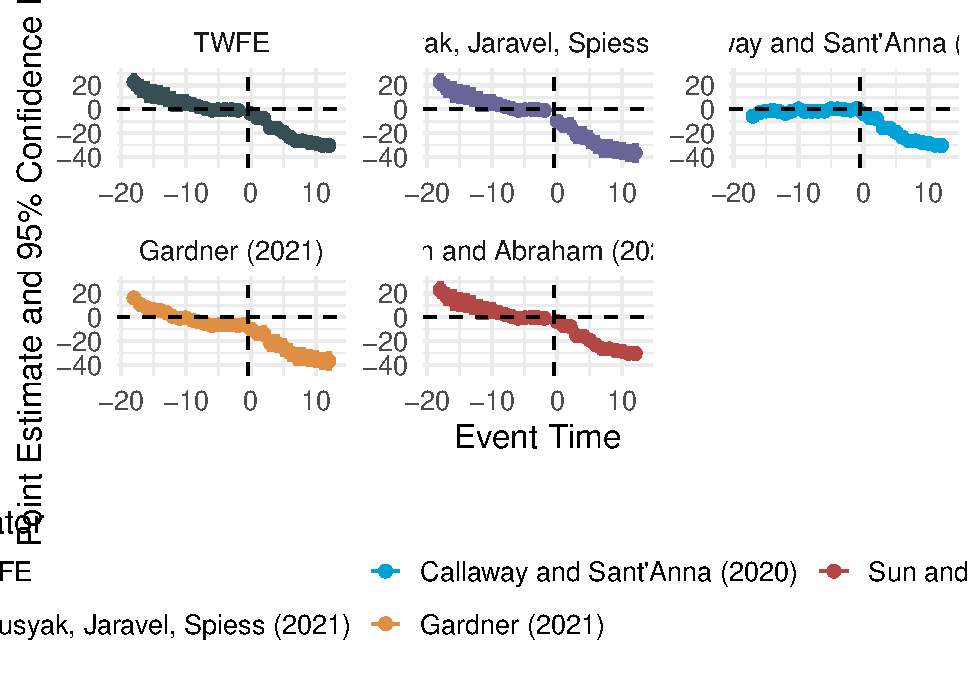
\includegraphics[keepaspectratio,alt={\label{fig:did1}Event study para o estimador de DiD aplicado ao exemplo da Califórnia.}]{bookdownproj_files/figure-latex/did1-1.pdf}}
\caption{\label{fig:did1}Event study para o estimador de DiD aplicado ao exemplo da Califórnia.}
\end{figure}

Agora comparamos os três estimadores com o pacote \texttt{synthdid}:

\begin{Shaded}
\begin{Highlighting}[]
\FunctionTok{library}\NormalTok{(synthdid)}

\NormalTok{estimators }\OtherTok{=} \FunctionTok{list}\NormalTok{(}\AttributeTok{did=}\NormalTok{did\_estimate,}
                  \AttributeTok{sc=}\NormalTok{sc\_estimate,}
                  \AttributeTok{sdid=}\NormalTok{synthdid\_estimate)}

\NormalTok{df\_sdid }\OtherTok{\textless{}{-}}\NormalTok{ df }\SpecialCharTok{\%\textgreater{}\%}
\NormalTok{  dplyr}\SpecialCharTok{::}\FunctionTok{select}\NormalTok{(state, year, cigsale, treatment) }\SpecialCharTok{\%\textgreater{}\%}
  \FunctionTok{mutate}\NormalTok{(}\AttributeTok{treatment =} \FunctionTok{as.integer}\NormalTok{(treatment),}
         \AttributeTok{year =} \FunctionTok{as.integer}\NormalTok{(year),}
         \AttributeTok{state =} \FunctionTok{as.factor}\NormalTok{(state)) }\SpecialCharTok{\%\textgreater{}\%}
  \FunctionTok{as.data.frame}\NormalTok{()}

\NormalTok{setup }\OtherTok{\textless{}{-}} \FunctionTok{panel.matrices}\NormalTok{(df\_sdid)}

\NormalTok{estimates }\OtherTok{\textless{}{-}} \FunctionTok{lapply}\NormalTok{(estimators, }\ControlFlowTok{function}\NormalTok{(estimator) \{ }\FunctionTok{estimator}\NormalTok{(setup}\SpecialCharTok{$}\NormalTok{Y,}
\NormalTok{                                                               setup}\SpecialCharTok{$}\NormalTok{N0, setup}\SpecialCharTok{$}\NormalTok{T0) \} )}

\NormalTok{standard.errors }\OtherTok{=} \FunctionTok{mapply}\NormalTok{(}\ControlFlowTok{function}\NormalTok{(estimate, name) \{}
  \FunctionTok{set.seed}\NormalTok{(}\DecValTok{12345}\NormalTok{)}
  \ControlFlowTok{if}\NormalTok{(name }\SpecialCharTok{==} \StringTok{\textquotesingle{}mc\textquotesingle{}}\NormalTok{) \{ }\FunctionTok{mc\_placebo\_se}\NormalTok{(setup}\SpecialCharTok{$}\NormalTok{Y, setup}\SpecialCharTok{$}\NormalTok{N0, setup}\SpecialCharTok{$}\NormalTok{T0) \}}
  \ControlFlowTok{else}\NormalTok{ \{             }\FunctionTok{sqrt}\NormalTok{(}\FunctionTok{vcov}\NormalTok{(estimate, }\AttributeTok{method=}\StringTok{\textquotesingle{}placebo\textquotesingle{}}\NormalTok{))     \}}
\NormalTok{\}, estimates, }\FunctionTok{names}\NormalTok{(estimators))}

\CommentTok{\# Resultados}
\FunctionTok{data.frame}\NormalTok{(}
  \AttributeTok{Estimador =} \FunctionTok{c}\NormalTok{(}\StringTok{"DiD"}\NormalTok{, }\StringTok{"SC"}\NormalTok{, }\StringTok{"SDiD"}\NormalTok{),}
  \AttributeTok{ATT =} \FunctionTok{round}\NormalTok{(}\FunctionTok{sapply}\NormalTok{(estimates, }\ControlFlowTok{function}\NormalTok{(x) x[}\DecValTok{1}\NormalTok{]), }\DecValTok{2}\NormalTok{),}
  \AttributeTok{SE =} \FunctionTok{round}\NormalTok{(standard.errors, }\DecValTok{2}\NormalTok{)}
\NormalTok{) }\SpecialCharTok{\%\textgreater{}\%}
  \FunctionTok{kable}\NormalTok{(}\AttributeTok{caption =} \StringTok{"Estimativas de ATT e erros{-}padrão para DiD, controle sintético e Synthetic DiD."}\NormalTok{)}
\end{Highlighting}
\end{Shaded}

\begin{table}

\caption{\label{tab:sdid}Estimativas de ATT e erros-padrão para DiD, controle sintético e Synthetic DiD.}
\centering
\begin{tabular}[t]{l|l|r|r}
\hline
  & Estimador & ATT & SE\\
\hline
did & DiD & -27.35 & 17.74\\
\hline
sc & SC & -19.62 & 9.92\\
\hline
sdid & SDiD & -15.60 & 8.37\\
\hline
\end{tabular}
\end{table}

O gráfico a seguir compara visualmente as trajetórias estimadas:

\begin{Shaded}
\begin{Highlighting}[]
\FunctionTok{synthdid\_plot}\NormalTok{(estimates[}\DecValTok{1}\SpecialCharTok{:}\DecValTok{3}\NormalTok{], }\AttributeTok{facet.vertical=}\ConstantTok{FALSE}\NormalTok{,}
              \AttributeTok{control.name=}\StringTok{\textquotesingle{}control\textquotesingle{}}\NormalTok{, }\AttributeTok{treated.name=}\StringTok{\textquotesingle{}california\textquotesingle{}}\NormalTok{,}
              \AttributeTok{lambda.comparable=}\ConstantTok{TRUE}\NormalTok{, }\AttributeTok{se.method =} \StringTok{\textquotesingle{}none\textquotesingle{}}\NormalTok{,}
              \AttributeTok{trajectory.linetype =} \DecValTok{1}\NormalTok{, }\AttributeTok{line.width=}\NormalTok{.}\DecValTok{75}\NormalTok{, }\AttributeTok{effect.curvature=}\SpecialCharTok{{-}}\NormalTok{.}\DecValTok{4}\NormalTok{,}
              \AttributeTok{trajectory.alpha=}\NormalTok{.}\DecValTok{7}\NormalTok{, }\AttributeTok{effect.alpha=}\NormalTok{.}\DecValTok{7}\NormalTok{,}
              \AttributeTok{diagram.alpha=}\DecValTok{1}\NormalTok{, }\AttributeTok{onset.alpha=}\NormalTok{.}\DecValTok{7}\NormalTok{) }\SpecialCharTok{+}
  \FunctionTok{theme}\NormalTok{(}\AttributeTok{legend.position=}\FunctionTok{c}\NormalTok{(.}\DecValTok{26}\NormalTok{,.}\DecValTok{07}\NormalTok{), }\AttributeTok{legend.direction=}\StringTok{\textquotesingle{}horizontal\textquotesingle{}}\NormalTok{,}
        \AttributeTok{legend.key=}\FunctionTok{element\_blank}\NormalTok{(), }\AttributeTok{legend.background=}\FunctionTok{element\_blank}\NormalTok{(),}
        \AttributeTok{strip.background=}\FunctionTok{element\_blank}\NormalTok{(), }\AttributeTok{strip.text.x =} \FunctionTok{element\_blank}\NormalTok{())}
\end{Highlighting}
\end{Shaded}

\begin{figure}
\centering
\pandocbounded{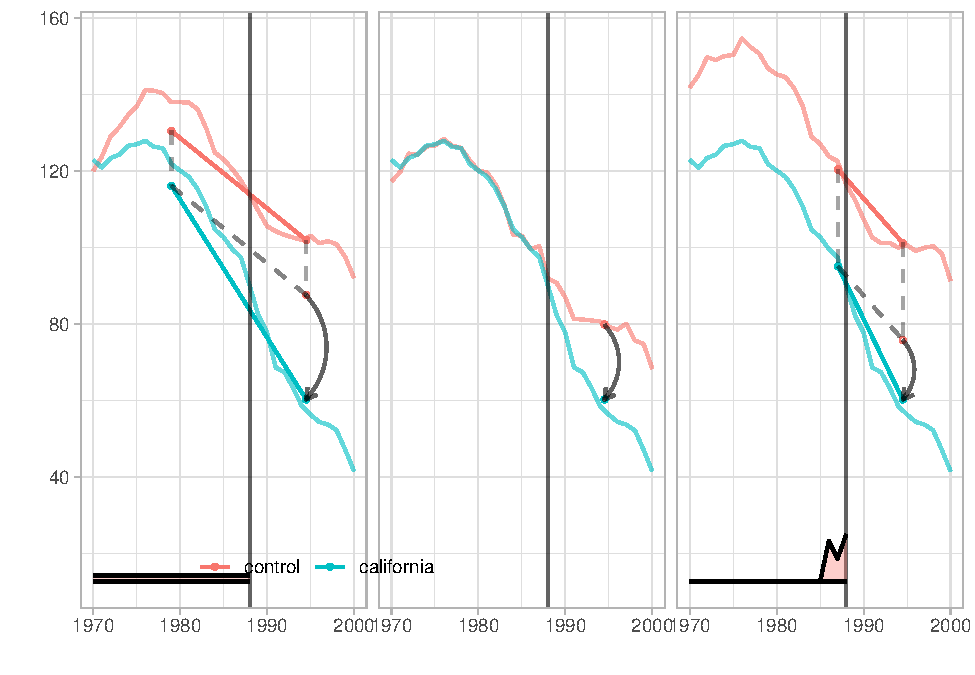
\includegraphics[keepaspectratio,alt={\label{fig:sdid1}Comparação visual das trajetórias estimadas por DiD, controle sintético e Synthetic DiD.}]{bookdownproj_files/figure-latex/sdid1-1.pdf}}
\caption{\label{fig:sdid1}Comparação visual das trajetórias estimadas por DiD, controle sintético e Synthetic DiD.}
\end{figure}

E os pesos de unidade atribuídos por cada estimador:

\begin{Shaded}
\begin{Highlighting}[]
\FunctionTok{synthdid\_units\_plot}\NormalTok{(}\FunctionTok{rev}\NormalTok{(estimates[}\DecValTok{1}\SpecialCharTok{:}\DecValTok{3}\NormalTok{]), }\AttributeTok{se.method=}\StringTok{\textquotesingle{}none\textquotesingle{}}\NormalTok{)}
\end{Highlighting}
\end{Shaded}

\begin{figure}
\centering
\pandocbounded{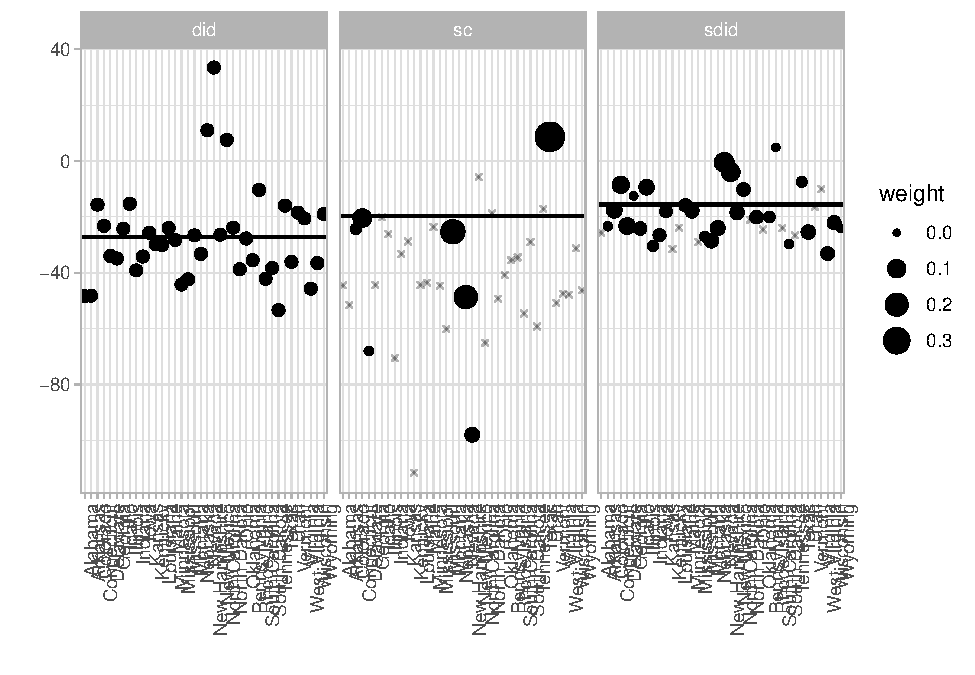
\includegraphics[keepaspectratio,alt={\label{fig:sdid2}Pesos de unidade atribuídos por DiD, controle sintético e Synthetic DiD.}]{bookdownproj_files/figure-latex/sdid2-1.pdf}}
\caption{\label{fig:sdid2}Pesos de unidade atribuídos por DiD, controle sintético e Synthetic DiD.}
\end{figure}

Note que o DiD atribui peso igual a todos os estados de controle, o SC concentra peso em poucos estados similares à Califórnia, e o SDiD faz algo intermediário.

\subsection{TROP: estimador triplamente robusto}\label{trop-estimador-triplamente-robusto}

Athey, Imbens, Qu e Viviano (2025) propõem o \textbf{TROP} (\emph{Triply Robust Panel Estimator}), que combina três componentes:

\begin{enumerate}
\def\labelenumi{\arabic{enumi}.}
\tightlist
\item
  Um \textbf{modelo de fatores} (outcome model): \(Y_{it}(0) = \mu_i + \lambda'_i f_t + \varepsilon_{it}\)
\item
  \textbf{Pesos de unidade} \(w_i\) (análogo ao SCM)
\item
  \textbf{Pesos temporais} \(\omega_t\) (análogo ao SDiD)
\end{enumerate}

A propriedade central do TROP é a \textbf{tripla robustez}. Para entender essa propriedade, considere que o viés do estimador tem uma estrutura \emph{multiplicativa}: é proporcional ao produto de três termos de erro de especificação:
\[
\text{viés} \propto e_{\text{modelo}} \times e_{\text{pesos de unidade}} \times e_{\text{pesos temporais}}
\]

onde \(e_{\text{modelo}}\) é o erro do modelo de fatores, \(e_{\text{pesos de unidade}}\) é o erro dos pesos de unidade, e \(e_{\text{pesos temporais}}\) é o erro dos pesos temporais. Como o viés é um \emph{produto} desses três termos, basta que \emph{qualquer um} deles seja zero para que o viés total desapareça. Em outras palavras, o estimador é consistente se qualquer um dos três componentes estiver corretamente especificado --- não é necessário que todos estejam corretos simultaneamente.

Isso contrasta com o SDiD, que usa efeitos fixos aditivos + pesos, enquanto o TROP usa um modelo de fatores + pesos. Contudo, é importante notar que quando \emph{todos os três} componentes estão mal especificados, o viés pode ser arbitrário --- a tripla robustez não protege contra falha simultânea de todos os componentes.

Em simulações, Athey et al.~(2025) mostram que o TROP supera substancialmente o TWFE e compete com o SDiD e o MC em uma variedade de cenários. A recomendação dos autores é usar simulações calibradas aos dados para escolher entre estimadores --- não há estimador que domine em todos os cenários.

\textbf{Nota}: o artigo de Athey et al.~(2025) é um \emph{preprint} que ainda não passou por revisão por pares. Até 2026, não existe pacote R público para o TROP. A menção aqui é teórica e serve para situar o leitor na fronteira da literatura.

\subsection{Quando usar cada método: guia prático}\label{quando-usar-cada-muxe9todo-guia-pruxe1tico}

A escolha entre os métodos depende do contexto empírico. Eis um guia baseado nas recomendações de Liu et al.~(2024, p.~175):

\textbf{Árvore de decisão:}

\begin{enumerate}
\def\labelenumi{\arabic{enumi}.}
\tightlist
\item
  \textbf{Uma única unidade tratada} → SCM (seção 2) ou SCM aumentado (Ben-Michael et al., 2021)
\item
  \textbf{Múltiplas unidades, tendências paralelas plausíveis} → DiD/FEct (capítulo 8 e seção 5.1)
\item
  \textbf{Múltiplas unidades, tendências paralelas duvidosas} → IFEct ou MC (seção 5.2--5.3)
\item
  \textbf{Poucas unidades de controle} → SDiD (seção 7) --- os pesos ajudam a criar comparabilidade
\end{enumerate}

\textbf{Checklist prático} (adaptado de Liu et al., 2024):

\begin{enumerate}
\def\labelenumi{\arabic{enumi}.}
\tightlist
\item
  Visualize o \emph{treatment status}: quando cada unidade entra no tratamento?
\item
  Visualize a variável resposta: há tendências não-paralelas visíveis?
\item
  Comece com FEct + diagnósticos (placebo test, equivalência)
\item
  Se os diagnósticos falharem → tente IFEct ou MC + diagnósticos
\item
  Se houver carryover → remova os períodos afetados e reestime
\item
  Compare as estimativas entre métodos: se concordarem, há robustez; se divergirem, investigue por quê
\end{enumerate}

A tabela abaixo resume as suposições e características de cada método:

\begin{table}

\caption{\label{tab:tabela-guia-metodos-scm}Resumo das suposições, pesos e pacotes dos principais estimadores contrafactuais discutidos no capítulo.}
\centering
\begin{tabular}[t]{l|l|l|l|l}
\hline
Método & Modelo para $Y(0)$ & Relaxa tendências paralelas? & Pesos & Pacote R\\
\hline
DiD/TWFE & $\alpha_i + \lambda_t$ & Não & Iguais & fixest\\
\hline
FEct & $X'\beta + \alpha_i + \xi_t$ & Não (mesma suposição) & Uniformes & fect\\
\hline
IFEct & $X'\beta + \alpha_i + \xi_t + \lambda'_i f_t$ & Sim (fatores) & Uniformes & fect\\
\hline
MC & Baixo posto (norma nuclear) & Sim (baixo posto) & Implícitos (norma nuclear) & fect\\
\hline
SCM & Combinação convexa & Indiretamente (via pesos) & Convexos & tidysynth\\
\hline
SDiD & $\alpha_i + \lambda_t$ + pesos & Indiretamente (via pesos) & Unid. + tempo & synthdid\\
\hline
TROP & Fatores + pesos & Sim (tripla robustez) & Unid. + tempo & Sem pacote público até 2026\\
\hline
\end{tabular}
\end{table}

A relação entre esses métodos envolve duas dimensões distintas. A primeira é a \textbf{flexibilidade do modelo}: DiD/FEct assumem efeitos aditivos, enquanto IFEct e MC permitem estrutura de fatores (baixo posto), relaxando tendências paralelas. A segunda é a \textbf{robustez à má especificação}: o SDiD usa o mesmo modelo aditivo do FEct, mas adiciona pesos de unidade e temporais que o tornam mais robusto quando tendências paralelas globais falham --- é mais robusto, não necessariamente mais flexível. Da mesma forma, o TROP não relaxa suposições além do modelo de fatores; sua contribuição é a tripla robustez via estrutura multiplicativa do viés, que o protege contra erros em qualquer um dos três componentes. MC e IFEct operam sob suposições de baixo posto similares, mas diferem computacionalmente (\emph{soft} vs.~\emph{hard impute}). Em todos os casos, métodos com menos suposições ou mais robustez tendem a pagar um custo em variância: a escolha envolve o trade-off viés-variância usual.

\subsection{Resumo}\label{resumo-2}

Neste capítulo, apresentamos uma família de métodos para estimação de efeitos causais em dados de painel, unificados pela ideia de \textbf{imputação do contrafactual} \(Y_{it}(0)\):

\begin{itemize}
\tightlist
\item
  O \textbf{SCM} constrói o contrafactual como combinação convexa de unidades não-tratadas --- ideal para estudos de caso com uma unidade tratada.
\item
  O \textbf{framework de estimação contrafactual} (Liu et al., 2024) generaliza a imputação para três estimadores (FEct, IFEct, MC) com diagnósticos formais.
\item
  O \textbf{SDiD} combina pesos de unidade e temporais com efeitos fixos, criando tendências paralelas localmente.
\item
  O \textbf{TROP} (Athey et al., 2025) oferece tripla robustez combinando modelo de fatores com pesos de unidade e pesos temporais.
\end{itemize}

A conexão com o capítulo 8 (DiD) é direta: o FEct é equivalente ao DiD por imputação de Borusyak et al.~(2024), e o DiD tradicional é um caso especial do framework quando \(h(U_{it}) = \alpha_i + \xi_t\). A conexão com o capítulo 9 (TSCS) também é clara: o IFEct estende os modelos de fatores interativos de Xu (2017) e Gobillon e Magnac (2016) para o contexto de inferência causal.

\subsection{Referências}\label{referuxeancias-3}

Abadie, A. (2021). Using synthetic controls: Feasibility, data requirements, and methodological aspects. \emph{Journal of Economic Literature}, 59(2), 391--425.

Abadie, A., \& Gardeazabal, J. (2003). The economic costs of conflict: A case study of the Basque Country. \emph{American Economic Review}, 93(1), 113--132.

Abadie, A., Diamond, A., \& Hainmueller, J. (2010). Synthetic control methods for comparative case studies: Estimating the effect of California's tobacco control program. \emph{Journal of the American Statistical Association}, 105(490), 493--505.

Abadie, A., Diamond, A., \& Hainmueller, J. (2015). Comparative politics and the synthetic control method. \emph{American Journal of Political Science}, 59(2), 495--510.

Abadie, A., \& L'Hour, J. (2021). A penalized synthetic control estimator for disaggregated data. \emph{Journal of the American Statistical Association}, 116(536), 1817--1834.

Arkhangelsky, D., Athey, S., Hirshberg, D. A., Imbens, G. W., \& Wager, S. (2021). Synthetic difference-in-differences. \emph{American Economic Review}, 111(12), 4088--4118.

Arkhangelsky, D., \& Imbens, G. (2024). Causal models for longitudinal and panel data: A survey. \emph{The Econometrics Journal}, 27(3), C1--C61.

Athey, S., Bayati, M., Doudchenko, N., Imbens, G., \& Khosravi, K. (2021). Matrix completion methods for causal panel data models. \emph{Journal of the American Statistical Association}, 116(536), 1716--1730.

Athey, S., Imbens, G., Qu, Z., \& Viviano, D. (2025). Triply robust estimation of causal effects with missing data in panel studies. Preprint.

Ben-Michael, E., Feller, A., \& Rothstein, J. (2021). The augmented synthetic control method. \emph{Journal of the American Statistical Association}, 116(536), 1789--1803.

Borusyak, K., Jaravel, X., \& Spiess, J. (2024). Revisiting event-study designs: Robust and efficient estimation. \emph{Review of Economic Studies}, 91(6), 3253--3285.

Chernozhukov, V., Wüthrich, K., \& Zhu, Y. (2021). An exact and robust conformal inference method for counterfactual and synthetic controls. \emph{Journal of the American Statistical Association}, 116(536), 1849--1864.

Doudchenko, N., \& Imbens, G. W. (2016). Balancing, regression, difference-in-differences and synthetic control methods: A synthesis. Working Paper 22791, National Bureau of Economic Research.

Gobillon, L., \& Magnac, T. (2016). Regional policy evaluation: Interactive fixed effects and synthetic controls. \emph{Review of Economics and Statistics}, 98(3), 535--551.

Kaul, A., Klößner, S., Pfeifer, G., \& Schieler, M. (2022). Standard synthetic control methods: The case of using all preintervention outcomes together with covariates. \emph{Journal of Business \& Economic Statistics}, 40(3), 1362--1376.

Liu, L., Wang, Y., \& Xu, Y. (2024). A practical guide to counterfactual estimators for causal inference with time-series cross-sectional data. \emph{American Journal of Political Science}, 68(1), 160--176.

Robbins, M. W., Saunders, J., \& Kilmer, B. (2017). A framework for synthetic control methods with high-dimensional, micro-level data: Evaluating a neighborhood-specific crime intervention. \emph{Journal of the American Statistical Association}, 112(517), 109--126.

Xu, Y. (2017). Generalized synthetic control method: Causal inference with interactive fixed effects models. \emph{Political Analysis}, 25(1), 57--76.

\section{LLMs e outras}\label{llms-e-outras}

\subsection{Google Colab}\label{google-colab}

Para a aula de hoje, vamos usar o Google Colab, que é uma ferramenta online, gratuita, para programar e analisar dados. Ela permite escrever e rodar códigos em Python sem a necessidade de instalar nenhum programa. Além disso, é possível ter acesso a processadores poderosos, inclusive de GPUs, se necessário (mas pagando).

Para usar o Google Colab, precisamos de uma conta Google, o que nós já temos com nosso e-mail usp.
Vamos acessar o endereço: \url{https://colab.google}

Vamos clicar em new notebook.
Vamos renomear o arquivo para aula\_llm.ipynb

A terminação diz que é um notebook. Que é como se fosse um Rmarkdown no R, só que nesse caso, hospedado online.

\url{https://macartan.github.io/dd_bootcamp/dd.html\#/using-a-design-1}
\url{https://macartan.github.io/dd_bootcamp/exercises.html}
\url{https://gist.github.com/saudiwin/dd0edec5786c7edb393bd84615aafb45}

\url{https://www.datacamp.com/tutorial/fine-tuning-openais-gpt-4-step-by-step-guide}
\url{https://community.revelo.com.br/tutorial-aplicacao-do-fine-tuning-para-treinamento-no-chatgpt/}

\section{Machine Learning}\label{machine-learning}

\subsection{Introdução}\label{introduuxe7uxe3o-7}

Em estudos observacionais, como vimos, análises baseadas no pressuposto de \emph{conditional ignorability} do tratamento e positividade permitem a estimação de quantidades causais de interesse.
As técnicas de machine learning foram desenvolvidas em geral voltadas para o problema de previsão, não de inferência causal. Por isso, não são normalmente uma alternativa boa para as questões de identificação causal que temos discutido no curso. Contudo, com algumas adaptações, podem ser usadas para análise de causa e efeito.

Uma das abordagens mais populares é a sugerida por Belloni et al.~(2014), de usar LASSO (Least Absolute Shrinkage and Selection Operator) para inferir causalidade.

\subsection{Terminologia}\label{terminologia}

Estatística Machine Learning

observações

\subsubsection{LASSO}\label{lasso}

O estimador de Mínimos Quadrados Ordinários é obtido minimizando a soma dos quadrados dos resíduos, isto é, em uma regressão \(y_i = \beta_0 + \beta_1 x_{1i} + \beta_2 x_{2i} + \ldots + \beta_p x_{pi} + e_i\), minimizamos \(\sum_{i=1}^n [y_i - (\alpha + \beta_1x_{1i} + \beta_2 x_{2i} + \ldots + \beta_px_{pi})]^2\). Nós podemos pensar essa minimização como uma função de custo. Quanto menor o erro total, menor o custo.

O estimador de LASSO adiciona uma penalidade a essa função de minimização \(\lambda \sum_{j=1}^p |\beta_j|\), ou seja, passamos a minimizar: \(\sum_{i=1}^n [y_i - (\alpha + \beta_1x_{1i} + \beta_2x_{2i} + \ldots + \beta_px_{pi})]^2 + \lambda \sum_{j=1}^p |\beta_j|\)

O termo \(\sum_{j=1}^p |\beta_j|\) é chamado de norma L1. Ele envolve a soma absoluta dos parâmetros. Existem outras normas (L0, L2 etc.), isto é, outras formas de penalizar a estimação dos coeficientes. A norma L1 é conhecida como distância de Manhattan, e a intuição é que, se tenho dois pontos em Manhattan, \((x_1, y_1)\) e \((x_2, y_2)\), que são ruas em esquinas opostas de uma quadra (na diagonal). Como as ruas são, em geral, em formato de grade, temos de andar uma quadra na vertical e outra na horizontal para sair de um ponto a outro. Essa distância é a norma L1. Se usássemos a norma L2, por exemplo, poderíamos ir na diagonal, que é dada pela distância euclidiana.

E \(\lambda\) é um parâmetro não negativo que controla a força da penalização. Veja que coeficientes positivos dos \(\beta\) aumentam o custo total, de modo que eles precisam ser compensados pelo ganho gerado na capacidade preditiva da variável associada (quanto maior a correlação parcial, menor o erro). Assim, ao introduzir essa penalidade, o LASSO estimula que apenas as variáveis com maior capacidade preditiva possuam coeficientes positivos, enquanto as de baixa capacidade preditiva terão coeficiente igual a zero. Nós chamamos isso de esparsidade do vetor de coeficientes, já que muitos deles serão zero. Dizemos também que a regressão foi estimada com regularização. Veja que o LASSO é o equivalente a uma regressão Bayesiana com uma priori nos parâmetros igual a um dupla exponencial, levando à interpretação de que a priori é uma forma de regularizar estimativas.

Quando \(\lambda \to 0\), os coeficientes convergem para os estimadores de MQO, e quando \(\lambda \to \infty\) apenas o intercepto resta. Em ML, o método usual para achar \(\lambda\) é validação cruzada (CV, de cross-validation), que é utilizada para favorecer previsões fora da amostra. Belloni et al.~(2012) advogam uma escolha baseada em teoria, também conhecido como LASSO rigoroso. Angrist \& Frandsen (2022) concluíram que essa abordagem rigorosa tende a favorecer modelos mais parsimoniosos (\(\lambda\) maiores) do que com CV.

\subsubsection{Double Lasso}\label{double-lasso}

O estimador robusto mais popular é o Double Lasso. A ideia é que se eu tentar usar LASSO diretamente na equação de regressão \(y_i = \alpha + \beta_1D_i + BX + e_i\), variáveis correlacionadas entre si terão coeficientes zero, e potencialmente o tratamento será uma delas, impedindo a estimação da quantidade causal de interesse. Estratégias como forçar \(D_i\) a permanecer na equação implicam que ficará fora da equação de penalização. Contudo, isso pode causar viés na estimação de \(\beta_1\) (Belloni et al., 2014). Essa regularização força variáveis correlacionadas com o tratamento a serem dropadas, o que significa dropar potenciais variáveis de confusão.

Resumo: não use as técnicas de ML diretamente na equação de regressão.

Exemplo.

\begin{Shaded}
\begin{Highlighting}[]
\CommentTok{\# vou rodar mil simulações com n=100}
\FunctionTok{set.seed}\NormalTok{(}\DecValTok{10}\NormalTok{)}
\NormalTok{k }\OtherTok{\textless{}{-}} \DecValTok{90} \CommentTok{\# número de controles}
\NormalTok{n }\OtherTok{\textless{}{-}} \DecValTok{100} \CommentTok{\# número de obs}
\NormalTok{alpha }\OtherTok{\textless{}{-}}\NormalTok{ .}\DecValTok{2} \CommentTok{\# intercepto}
\NormalTok{beta }\OtherTok{\textless{}{-}} \DecValTok{0} \CommentTok{\# efeito do tratamento}
\NormalTok{gamma }\OtherTok{\textless{}{-}} \FunctionTok{runif}\NormalTok{(}\AttributeTok{min=}\SpecialCharTok{{-}}\DecValTok{1}\NormalTok{, }\AttributeTok{max=}\DecValTok{1}\NormalTok{, }\AttributeTok{n=}\NormalTok{k) }\CommentTok{\# efeito do vetor de controles}
\NormalTok{delta }\OtherTok{\textless{}{-}} \FunctionTok{runif}\NormalTok{(}\AttributeTok{min=}\SpecialCharTok{{-}}\DecValTok{1}\NormalTok{, }\AttributeTok{max=}\DecValTok{1}\NormalTok{, }\AttributeTok{n=}\NormalTok{k) }
\NormalTok{erro }\OtherTok{\textless{}{-}} \FunctionTok{rnorm}\NormalTok{(n)}
\NormalTok{vec\_x }\OtherTok{\textless{}{-}} \FunctionTok{rnorm}\NormalTok{(n}\SpecialCharTok{*}\NormalTok{k, }\AttributeTok{mean =} \FunctionTok{rep}\NormalTok{(}\DecValTok{0}\NormalTok{,k)) }\CommentTok{\# vetor de controles}
\NormalTok{x }\OtherTok{\textless{}{-}} \FunctionTok{matrix}\NormalTok{(vec\_x, }\AttributeTok{ncol=}\NormalTok{k)}
\NormalTok{D }\OtherTok{\textless{}{-}}\NormalTok{ x}\SpecialCharTok{\%*\%}\NormalTok{delta }\SpecialCharTok{+} \FunctionTok{rnorm}\NormalTok{(n)}
\NormalTok{y }\OtherTok{\textless{}{-}}\NormalTok{ alpha }\SpecialCharTok{+}\NormalTok{ beta}\SpecialCharTok{*}\NormalTok{D }\SpecialCharTok{+}\NormalTok{ x}\SpecialCharTok{\%*\%}\NormalTok{gamma }\SpecialCharTok{+}\NormalTok{ erro}
\NormalTok{fit }\OtherTok{\textless{}{-}} \FunctionTok{lm}\NormalTok{(y }\SpecialCharTok{\textasciitilde{}}\NormalTok{D }\SpecialCharTok{+}\NormalTok{ x)}
\FunctionTok{coef}\NormalTok{(}\FunctionTok{summary}\NormalTok{(fit))[}\DecValTok{2}\NormalTok{]}
\end{Highlighting}
\end{Shaded}

\begin{Shaded}
\begin{Highlighting}[]
\FunctionTok{library}\NormalTok{(MASS)}
\end{Highlighting}
\end{Shaded}

\begin{verbatim}
## 
## Attaching package: 'MASS'
\end{verbatim}

\begin{verbatim}
## The following object is masked from 'package:dplyr':
## 
##     select
\end{verbatim}

\begin{Shaded}
\begin{Highlighting}[]
\FunctionTok{library}\NormalTok{(arm)}
\end{Highlighting}
\end{Shaded}

\begin{verbatim}
## Loading required package: Matrix
\end{verbatim}

\begin{verbatim}
## 
## Attaching package: 'Matrix'
\end{verbatim}

\begin{verbatim}
## The following objects are masked from 'package:tidyr':
## 
##     expand, pack, unpack
\end{verbatim}

\begin{verbatim}
## Loading required package: lme4
\end{verbatim}

\begin{verbatim}
## 
## arm (Version 1.14-4, built: 2024-4-1)
\end{verbatim}

\begin{verbatim}
## Working directory is /Users/manoelgaldino/Documents/DCP/Cursos/Causalidade/Causalidade
\end{verbatim}

\begin{verbatim}
## 
## Attaching package: 'arm'
\end{verbatim}

\begin{verbatim}
## The following object is masked from 'package:did':
## 
##     sim
\end{verbatim}

\begin{verbatim}
## The following object is masked from 'package:fixest':
## 
##     coefplot
\end{verbatim}

\begin{Shaded}
\begin{Highlighting}[]
\NormalTok{sim\_pvalue\_dl }\OtherTok{\textless{}{-}} \ControlFlowTok{function}\NormalTok{(}\AttributeTok{n\_sim=}\DecValTok{1000}\NormalTok{, }\AttributeTok{n\_sample=}\DecValTok{100}\NormalTok{) \{}
\NormalTok{  vec\_p\_values }\OtherTok{\textless{}{-}} \FunctionTok{numeric}\NormalTok{()}
\NormalTok{  beta\_hat }\OtherTok{\textless{}{-}} \FunctionTok{numeric}\NormalTok{()}
\NormalTok{  theta\_hat }\OtherTok{\textless{}{-}} \FunctionTok{numeric}\NormalTok{()}
\NormalTok{  lista\_df }\OtherTok{\textless{}{-}} \FunctionTok{list}\NormalTok{()}
  
  \ControlFlowTok{for}\NormalTok{ ( i }\ControlFlowTok{in} \DecValTok{1}\SpecialCharTok{:}\NormalTok{n\_sim) \{}
\NormalTok{k }\OtherTok{\textless{}{-}} \DecValTok{20} \CommentTok{\# número de controles}
\NormalTok{n }\OtherTok{\textless{}{-}}\NormalTok{ n\_sample }\CommentTok{\# número de obs}
\NormalTok{alpha }\OtherTok{\textless{}{-}}\NormalTok{ .}\DecValTok{2} \CommentTok{\# intercepto}
\NormalTok{beta }\OtherTok{\textless{}{-}} \DecValTok{0} \CommentTok{\# efeito do tratamento}
\NormalTok{theta }\OtherTok{\textless{}{-}} \DecValTok{1} \CommentTok{\# efeito D*V que nos interessa}
\NormalTok{gamma }\OtherTok{\textless{}{-}} \FunctionTok{runif}\NormalTok{(}\AttributeTok{min=}\SpecialCharTok{{-}}\DecValTok{1}\NormalTok{, }\AttributeTok{max=}\DecValTok{1}\NormalTok{, }\AttributeTok{n=}\NormalTok{k) }\CommentTok{\# efeito do vetor de controles no y}
\NormalTok{gamma[}\FunctionTok{sample}\NormalTok{(}\DecValTok{1}\SpecialCharTok{:}\NormalTok{k, (k}\SpecialCharTok{/}\DecValTok{4}\NormalTok{))] }\OtherTok{\textless{}{-}} \DecValTok{0} \CommentTok{\# k/4 zeros}
\NormalTok{delta }\OtherTok{\textless{}{-}} \FunctionTok{runif}\NormalTok{(}\AttributeTok{min=}\SpecialCharTok{{-}}\DecValTok{1}\NormalTok{, }\AttributeTok{max=}\DecValTok{1}\NormalTok{, }\AttributeTok{n=}\NormalTok{k) }\CommentTok{\# efeito do vetor de controles no D}
\NormalTok{erro }\OtherTok{\textless{}{-}} \FunctionTok{rnorm}\NormalTok{(n, }\DecValTok{0}\NormalTok{, }\DecValTok{5}\NormalTok{)}

\CommentTok{\# matriz de preditores correlacionados}
\NormalTok{rho   }\OtherTok{\textless{}{-}} \FloatTok{0.7}                         \CommentTok{\# correlação entre vizinhos imediatos}
\NormalTok{Sigma     }\OtherTok{\textless{}{-}} \FunctionTok{toeplitz}\NormalTok{(rho}\SpecialCharTok{\^{}}\NormalTok{(}\DecValTok{0}\SpecialCharTok{:}\NormalTok{(k}\DecValTok{{-}1}\NormalTok{)))     }\CommentTok{\# R\_\{ij\} = rho\^{}\{|i{-}j|\}, variâncias = 1}
\NormalTok{mean\_vector }\OtherTok{\textless{}{-}} \FunctionTok{rep}\NormalTok{(}\DecValTok{0}\NormalTok{, k)}
\NormalTok{x }\OtherTok{\textless{}{-}} \FunctionTok{mvrnorm}\NormalTok{(n, mean\_vector, Sigma)}
\NormalTok{x\_interaction }\OtherTok{\textless{}{-}}\NormalTok{ x[,}\DecValTok{10}\NormalTok{]}
\NormalTok{D }\OtherTok{\textless{}{-}} \FunctionTok{rbinom}\NormalTok{(n, }\DecValTok{1}\NormalTok{, }\FunctionTok{invlogit}\NormalTok{(x}\SpecialCharTok{\%*\%}\NormalTok{delta }\SpecialCharTok{+} \FunctionTok{rnorm}\NormalTok{(n)))}

\NormalTok{D\_num }\OtherTok{\textless{}{-}} \FunctionTok{as.numeric}\NormalTok{(D)                }\CommentTok{\# 0 ou 1}
\NormalTok{X     }\OtherTok{\textless{}{-}} \FunctionTok{as.matrix}\NormalTok{(x\_interaction)     }\CommentTok{\# 6 × 5 no seu exemplo}

\CommentTok{\# interação: cada linha multiplicada por D[i]}
\NormalTok{X\_int }\OtherTok{\textless{}{-}}\NormalTok{ X }\SpecialCharTok{*}\NormalTok{ D\_num }
\NormalTok{X\_int\_omitida }\OtherTok{\textless{}{-}}\NormalTok{ x\_interaction}\SpecialCharTok{*}\FunctionTok{as.matrix}\NormalTok{(x[,}\DecValTok{11}\SpecialCharTok{:}\DecValTok{20}\NormalTok{])}
\NormalTok{y }\OtherTok{\textless{}{-}}\NormalTok{ alpha }\SpecialCharTok{+}\NormalTok{ beta}\SpecialCharTok{*}\NormalTok{D }\SpecialCharTok{+}\NormalTok{ x}\SpecialCharTok{\%*\%}\NormalTok{gamma }\SpecialCharTok{+}\NormalTok{ X\_int}\SpecialCharTok{\%*\%}\NormalTok{theta }\SpecialCharTok{+} \FunctionTok{rowSums}\NormalTok{(X\_int\_omitida) }\SpecialCharTok{+}\NormalTok{ erro}
\NormalTok{df\_sim }\OtherTok{\textless{}{-}} \FunctionTok{data.frame}\NormalTok{(y, D, x, x\_interaction)}
\NormalTok{lista\_df[[i]] }\OtherTok{\textless{}{-}}\NormalTok{ df\_sim}
\NormalTok{fit }\OtherTok{\textless{}{-}} \FunctionTok{lm}\NormalTok{(y }\SpecialCharTok{\textasciitilde{}}\NormalTok{ D}\SpecialCharTok{*}\NormalTok{x\_interaction }\SpecialCharTok{+}\NormalTok{ x[,}\SpecialCharTok{{-}}\DecValTok{10}\NormalTok{], }\AttributeTok{data =}\NormalTok{ df\_sim)}
\NormalTok{beta\_hat[i] }\OtherTok{\textless{}{-}} \FunctionTok{coef}\NormalTok{(}\FunctionTok{summary}\NormalTok{(fit))[}\DecValTok{2}\NormalTok{]}
\NormalTok{vec\_p\_values[i] }\OtherTok{\textless{}{-}} \FunctionTok{summary}\NormalTok{(fit)}\SpecialCharTok{$}\NormalTok{coefficients[,}\DecValTok{4}\NormalTok{][}\DecValTok{2}\NormalTok{]}
\NormalTok{theta\_hat[i] }\OtherTok{\textless{}{-}} \FunctionTok{coef}\NormalTok{(}\FunctionTok{summary}\NormalTok{(fit))[}\DecValTok{3}\NormalTok{]}
\NormalTok{  \}}
  
\NormalTok{  df\_final }\OtherTok{\textless{}{-}} \FunctionTok{data.frame}\NormalTok{(}\AttributeTok{beta =}\NormalTok{ beta\_hat, }\AttributeTok{p\_values =}\NormalTok{ vec\_p\_values, }\AttributeTok{theta\_hat =}\NormalTok{ theta\_hat)}

  \FunctionTok{return}\NormalTok{(}\FunctionTok{list}\NormalTok{(}\AttributeTok{df\_final =}\NormalTok{ df\_final, }\AttributeTok{lista\_df =}\NormalTok{ lista\_df))}
\NormalTok{\}}

\NormalTok{result\_sim }\OtherTok{\textless{}{-}} \FunctionTok{sim\_pvalue\_dl}\NormalTok{()}
\NormalTok{my\_p\_values\_beta }\OtherTok{\textless{}{-}}\NormalTok{ result\_sim}\SpecialCharTok{$}\NormalTok{df\_final}
\NormalTok{lista\_df }\OtherTok{\textless{}{-}}\NormalTok{ result\_sim}\SpecialCharTok{$}\NormalTok{lista\_df}

\FunctionTok{hist}\NormalTok{(my\_p\_values\_beta}\SpecialCharTok{$}\NormalTok{p\_values, }\AttributeTok{breaks =} \DecValTok{30}\NormalTok{, }\AttributeTok{main =} \StringTok{"Teste de signific. de D"}\NormalTok{, }\AttributeTok{xlab =} \StringTok{"p{-}valor"}\NormalTok{)}
\FunctionTok{abline}\NormalTok{(}\AttributeTok{v =} \FloatTok{0.05}\NormalTok{, }\AttributeTok{col =} \StringTok{"red"}\NormalTok{, }\AttributeTok{lwd =} \DecValTok{1}\NormalTok{, }\AttributeTok{lty =} \DecValTok{1}\NormalTok{)}
\FunctionTok{text}\NormalTok{(}\FloatTok{0.1}\NormalTok{, }\FunctionTok{par}\NormalTok{(}\StringTok{"usr"}\NormalTok{)[}\DecValTok{4}\NormalTok{] }\SpecialCharTok{*} \FloatTok{0.75}\NormalTok{, }\StringTok{"0.05"}\NormalTok{, }\AttributeTok{col =} \StringTok{"red"}\NormalTok{, }\AttributeTok{pos =} \DecValTok{3}\NormalTok{, }\AttributeTok{cex=}\NormalTok{.}\DecValTok{5}\NormalTok{)}
\end{Highlighting}
\end{Shaded}

\pandocbounded{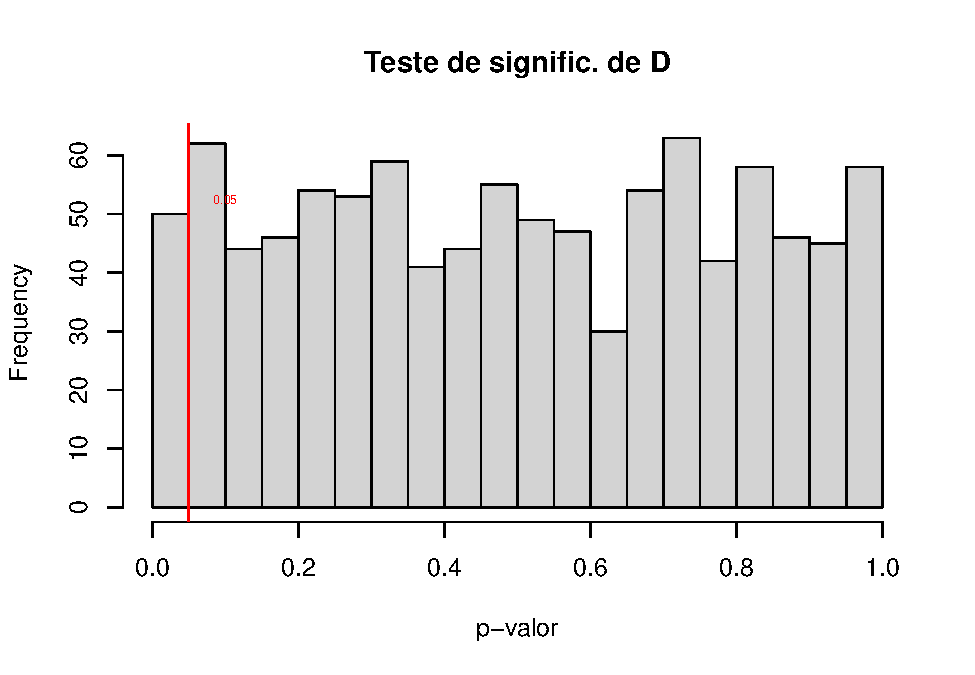
\includegraphics[keepaspectratio]{bookdownproj_files/figure-latex/cap13-sim2-1.pdf}}

\begin{Shaded}
\begin{Highlighting}[]
\FunctionTok{hist}\NormalTok{(my\_p\_values\_beta}\SpecialCharTok{$}\NormalTok{beta, }\AttributeTok{breaks =} \DecValTok{30}\NormalTok{, }\AttributeTok{main =} \StringTok{"Teste de signific. de D"}\NormalTok{, }\AttributeTok{xlab =} \StringTok{"p{-}valor"}\NormalTok{)}
\end{Highlighting}
\end{Shaded}

\pandocbounded{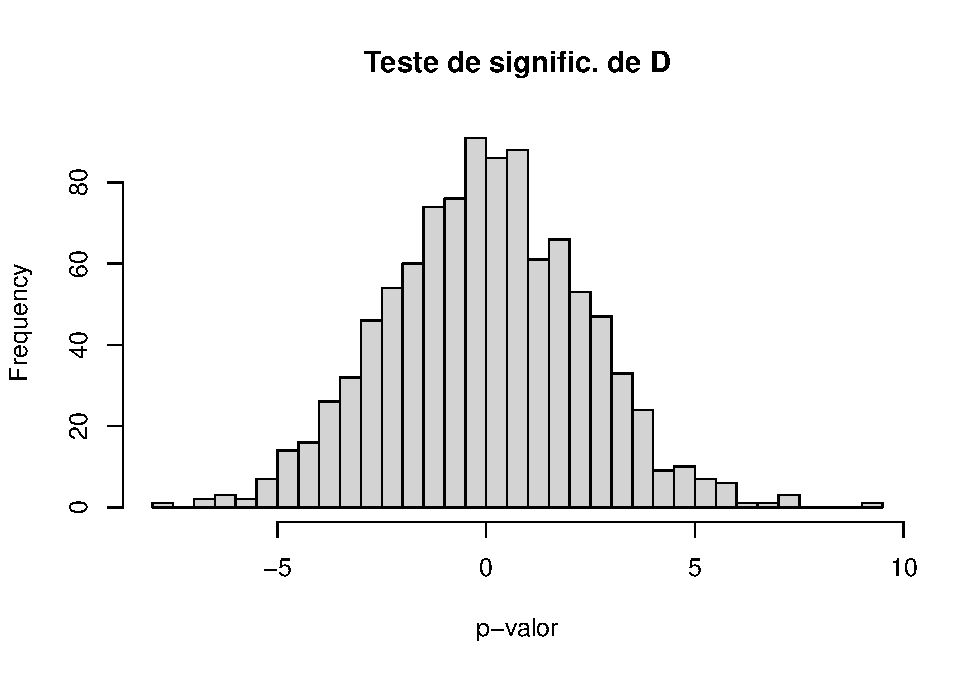
\includegraphics[keepaspectratio]{bookdownproj_files/figure-latex/cap13-sim2-2.pdf}}

\begin{Shaded}
\begin{Highlighting}[]
\CommentTok{\# percentual p{-}valor menor que 5\%}
\FunctionTok{sum}\NormalTok{(my\_p\_values\_beta}\SpecialCharTok{$}\NormalTok{p\_values }\SpecialCharTok{\textless{}=}\NormalTok{ .}\DecValTok{05}\NormalTok{)}\SpecialCharTok{/}\DecValTok{1000}
\end{Highlighting}
\end{Shaded}

\begin{verbatim}
## [1] 0.05
\end{verbatim}

\begin{Shaded}
\begin{Highlighting}[]
\FunctionTok{mean}\NormalTok{(my\_p\_values\_beta}\SpecialCharTok{$}\NormalTok{beta)}
\end{Highlighting}
\end{Shaded}

\begin{verbatim}
## [1] -0.0199413
\end{verbatim}

\begin{Shaded}
\begin{Highlighting}[]
\FunctionTok{mean}\NormalTok{(my\_p\_values\_beta}\SpecialCharTok{$}\NormalTok{theta\_hat)}
\end{Highlighting}
\end{Shaded}

\begin{verbatim}
## [1] -0.07478368
\end{verbatim}

Nós rejeitamos a hipótese nula aproximadamente 50\% do tempo.

E se usarmos LASSO (single LASSO)?

\begin{Shaded}
\begin{Highlighting}[]
\CommentTok{\# Instalar e carregar o pacote glmnet, se necessário}
\FunctionTok{library}\NormalTok{(glmnet)}
\end{Highlighting}
\end{Shaded}

\begin{verbatim}
## Loaded glmnet 4.1-9
\end{verbatim}

\begin{Shaded}
\begin{Highlighting}[]
\CommentTok{\# Vetor para armazenar se x foi selecionado pelo LASSO}
\NormalTok{lasso\_selected\_D }\OtherTok{\textless{}{-}} \FunctionTok{numeric}\NormalTok{()}

\CommentTok{\# Loop de simulação}
\ControlFlowTok{for}\NormalTok{ (i }\ControlFlowTok{in} \DecValTok{1}\SpecialCharTok{:}\DecValTok{1000}\NormalTok{) \{}
\NormalTok{  y }\OtherTok{\textless{}{-}}\NormalTok{ lista\_df[[i]]}\SpecialCharTok{$}\NormalTok{y}
\NormalTok{  X }\OtherTok{\textless{}{-}} \FunctionTok{cbind}\NormalTok{(lista\_df[[i]]}\SpecialCharTok{$}\NormalTok{D, lista\_df[[i]]}\SpecialCharTok{$}\NormalTok{x) }
  \CommentTok{\# Preparando os dados para o LASSO}
  \CommentTok{\# Matriz de preditores (sem o intercepto)}

  \CommentTok{\# Ajustando o modelo LASSO com validação cruzada}
\NormalTok{  lasso\_model }\OtherTok{\textless{}{-}} \FunctionTok{cv.glmnet}\NormalTok{(X, y, }\AttributeTok{alpha =} \DecValTok{1}\NormalTok{) }\CommentTok{\# alpha = 1 para LASSO}

  \CommentTok{\# Extraindo os coeficientes no valor de lambda que minimiza o erro}
\NormalTok{  lasso\_coefs }\OtherTok{\textless{}{-}} \FunctionTok{coef}\NormalTok{(lasso\_model, }\AttributeTok{s =} \StringTok{"lambda.min"}\NormalTok{)}

  \CommentTok{\# Verificando se a variável x foi selecionada pelo LASSO (coeficiente diferente de zero)}
\NormalTok{  lasso\_selected\_D[i] }\OtherTok{\textless{}{-}} \FunctionTok{ifelse}\NormalTok{(lasso\_coefs[}\StringTok{"V1"}\NormalTok{, }\DecValTok{1}\NormalTok{] }\SpecialCharTok{!=} \DecValTok{0}\NormalTok{, }\DecValTok{1}\NormalTok{, }\DecValTok{0}\NormalTok{)}
\NormalTok{\}}

\CommentTok{\# Analisando os resultados}
\FunctionTok{hist}\NormalTok{(lasso\_selected\_D, }\AttributeTok{breaks =} \DecValTok{40}\NormalTok{, }\AttributeTok{main =} \StringTok{"Seleção de x pelo LASSO"}\NormalTok{, }\AttributeTok{xlab =} \StringTok{"x selecionado (1 = sim, 0 = não)"}\NormalTok{)}
\end{Highlighting}
\end{Shaded}

\pandocbounded{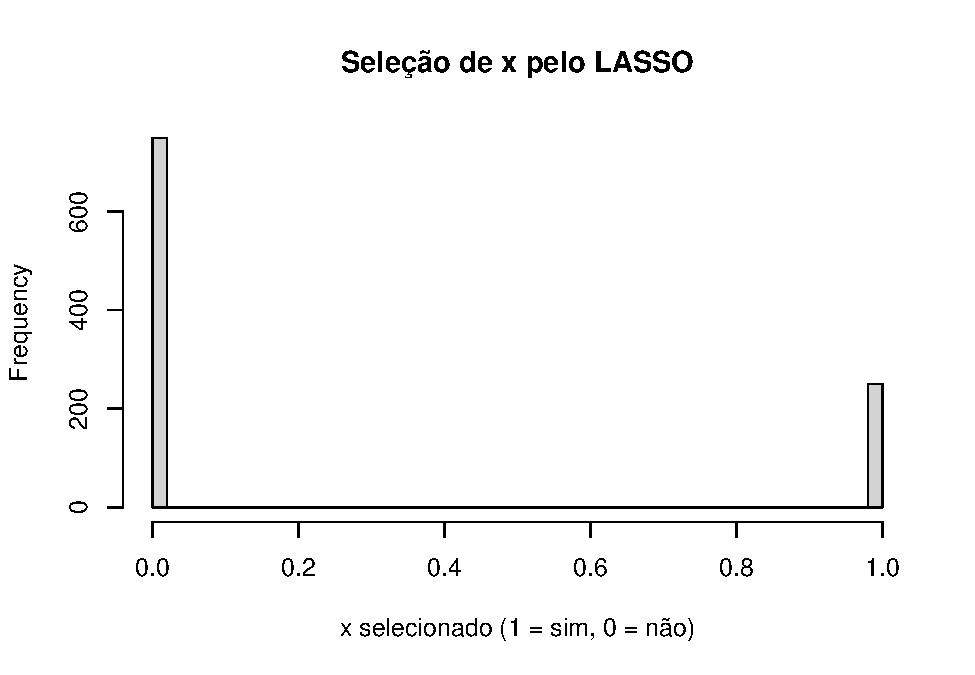
\includegraphics[keepaspectratio]{bookdownproj_files/figure-latex/cap13-sim3-1.pdf}}

\begin{Shaded}
\begin{Highlighting}[]
\FunctionTok{sum}\NormalTok{(lasso\_selected\_D }\SpecialCharTok{\textless{}=}\NormalTok{ .}\DecValTok{05}\NormalTok{)}\SpecialCharTok{/}\DecValTok{1000}
\end{Highlighting}
\end{Shaded}

\begin{verbatim}
## [1] 0.75
\end{verbatim}

Também não funciona, mais ou menos mesma taxa de erro.

\subsubsection{Outras soluções ineficazes}\label{outras-soluuxe7uxf5es-ineficazes}

Bootstrap (não funciona)
Clássico: suponha que a covariável não é relevante
Conservador: sempre inclua quantos controles puder (pode gerar Collider Bias).

DL lida com essa situação fazendo uma modelagem dupla, tanto do tratamento quanto da resposta. Daí o nome, Double Lasso.

\subsection{DL - Algoritmo}\label{dl---algoritmo}

Passo 1. Inclua controle se ele for preditor significativo da resposta \(y_i\) por um teste conservador (teste t, LASSO etc.)

Passo 2. Inclua controle se ele for preditor significativo do tratamento \(D_i\) por um teste conservador (teste t, LASSO etc.).

Passo 3. Ajuste o modelo com as variáveis selecionadas e o tratamento. Esse passo é chamado de Pós MQO (Post OLS).

No R, podemos usar o pacote ``hdm'' para fazer a implementação em uma linha.

\begin{Shaded}
\begin{Highlighting}[]
\FunctionTok{library}\NormalTok{(hdm)}
\FunctionTok{library}\NormalTok{(knitr)}
\NormalTok{d\_s\_vec }\OtherTok{\textless{}{-}} \FunctionTok{numeric}\NormalTok{()}
\ControlFlowTok{for}\NormalTok{ ( i }\ControlFlowTok{in} \DecValTok{1}\SpecialCharTok{:}\DecValTok{1000}\NormalTok{) \{}
\NormalTok{  my\_double\_selection }\OtherTok{\textless{}{-}} \FunctionTok{rlassoEffects}\NormalTok{(y}\SpecialCharTok{\textasciitilde{}}\NormalTok{. , }\AttributeTok{I=}\SpecialCharTok{\textasciitilde{}}\NormalTok{x }\SpecialCharTok{+}\NormalTok{ D, }\AttributeTok{data=}\NormalTok{lista\_df[[i]])}
\NormalTok{  d\_s\_vec[i] }\OtherTok{\textless{}{-}} \FunctionTok{summary}\NormalTok{(my\_double\_selection)}\SpecialCharTok{$}\NormalTok{coefficients[}\StringTok{"D"}\NormalTok{, }\StringTok{"Pr(\textgreater{}|t|)"}\NormalTok{]}
  
\NormalTok{\}}

\FunctionTok{hist}\NormalTok{(d\_s\_vec, }\AttributeTok{breaks =} \DecValTok{40}\NormalTok{, }\AttributeTok{main =} \StringTok{"Seleção de D pelo Double LASSO"}\NormalTok{, }\AttributeTok{xlab =} \StringTok{"p{-}valor"}\NormalTok{)}
\FunctionTok{abline}\NormalTok{(}\AttributeTok{v =} \FloatTok{0.05}\NormalTok{, }\AttributeTok{col =} \StringTok{"red"}\NormalTok{, }\AttributeTok{lwd =} \DecValTok{1}\NormalTok{, }\AttributeTok{lty =} \DecValTok{1}\NormalTok{)}
\FunctionTok{text}\NormalTok{(}\FloatTok{0.1}\NormalTok{, }\FunctionTok{par}\NormalTok{(}\StringTok{"usr"}\NormalTok{)[}\DecValTok{4}\NormalTok{] }\SpecialCharTok{*} \FloatTok{0.75}\NormalTok{, }\StringTok{"0.05"}\NormalTok{, }\AttributeTok{col =} \StringTok{"red"}\NormalTok{, }\AttributeTok{pos =} \DecValTok{3}\NormalTok{, }\AttributeTok{cex=}\NormalTok{.}\DecValTok{5}\NormalTok{)}
\end{Highlighting}
\end{Shaded}

\pandocbounded{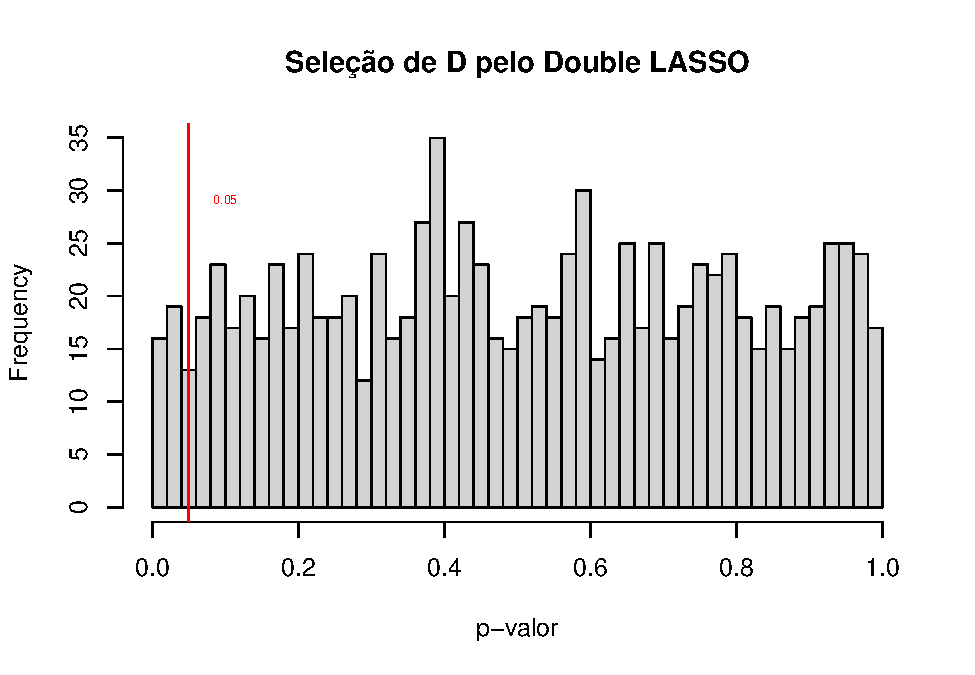
\includegraphics[keepaspectratio]{bookdownproj_files/figure-latex/cap-13-hdm-1.pdf}}

\begin{Shaded}
\begin{Highlighting}[]
\FunctionTok{sum}\NormalTok{(d\_s\_vec }\SpecialCharTok{\textless{}=}\NormalTok{ .}\DecValTok{05}\NormalTok{)}\SpecialCharTok{/}\DecValTok{1000}
\end{Highlighting}
\end{Shaded}

\begin{verbatim}
## [1] 0.04
\end{verbatim}

Como vemos, aproximadamente 5\% das vezes nós rejeitamos a hipótese nula erradamente, que é o esperado do p-valor de 5\%.

\subsection{Termos de Interação}\label{termos-de-interauxe7uxe3o}

Blackwell \& Olson (2022) argumentam que incluir um termo de interação com o tratamento, mas não com os controles, pode viesar as estimativas. Como eles falam: '' If the relationship between the covariates and the outcome also depends on the moderator {[}termo de interação{]}, a naive application of the single-interaction model can lead to what we call omitted interaction bias, a form of model misspecification that can be severe'' (p.~2).

A solução é usar o Double LASSO para escolher quais variáveis com termos de interação devem ser mantidas, e quais devem ser dropadas da regressão de especificação.

\subsection{Aplicação}\label{aplicauxe7uxe3o}

Alguns exemplos que encontrei em ciência política de aplicação do Double LASSO foram o artigo (working paper) de Dahlum et al.~(2024) e Dutt \& Tsetlin (2021).

O Double LASSO resolve o problema de seleção de variáveis para inferência causal. Uma abordagem mais geral, que permite o uso de qualquer método de Machine Learning para estimar os parâmetros de nuisance, é o Double/Debiased Machine Learning.

\subsection{DML}\label{dml}

A estratégia de identificação canônica em nosso curso tem girado sempre em torno de suposições críveis de identificação do efeito de um tratamento (em geral binário) \(D\) sobre a variável resposta (em geral contínua) \(Y\). E com frequência precisamos empregar controles para garantir a identificação causal e fechar as portas abertas (back-doors). Nesse contexto, as variáveis de controle são o que chamamos de \emph{nuisance variables}, isto é, variáveis que não são de interesse para a pergunta de pesquisa, mas que precisam ser levadas em consideração para que possamos estimar sem viés o parâmetro de interesse.

Considere o modelo de regressão padrão em um estudo observacional:

\(y_i = \alpha + \beta_1D_i + BX + e_i\), em que \(D_i\) é o tratamento (binário) e \(X\) é um vetor de \(p\) potenciais variáveis de confusão: \(\mathbf{X} = (x_1, x_2, \ldots, x_p)\) e \(B\) o vetor de parâmetros das variáveis de controle.

Dado que a regressão está aproximando uma esperança condicional \(\mathbb{E}[Y|D=d, \mathbf{X}= \mathbf{x}]\), ela pode ser escrita como:

\(\mathbb{E}[Y|D=d, \mathbf{X}= \mathbf{x}] = \eta_0(\mathbf{X}) + \theta_0(\mathbf{X})d\), em que \(\eta_0 = \mathbb{E}[Y|D=0, \mathbf{X}= \mathbf{x}]\) é um \emph{functional nuisance} e \(\theta_0 = \mathbb{E}[Y|D=1, \mathbf{X}= \mathbf{x}] - \mathbb{E}[Y|D=0, \mathbf{X}= \mathbf{x}]\) é o funcional de interesse.

Tipicamente, quando usamos regressão linear, estamos assumindo uma forma funcional específica para a função de \emph{nuisance}. Se houver erro de especificação, iremos introduzir um viés na estimativa do parâmetro de interesse. Aí é que entra o Double/Debiased Machine Learning.

\subsection{Double Debiasing}\label{double-debiasing}

O chamado Double/Debiased Machine Learning (DML) foi desenvolvido por Chernozhukov et al.~(2018). Sua inspiração vem do teorema de Frisch-Waugh-Lovell (FWL). Vamos começar por ele. Suponha o seguinte modelo de regressão múltipla:

\[
Y = \beta_0 + \beta_1X + \beta_2W_1 + \dots + \beta_{k+1}W_k + \epsilon
\]
Em que \(X\) é a variável causal de interesse (tratamento) e os \(W\) são variáveis de controle. São as \emph{nuisance variables}. O teorema de FWL diz que posso estimar \(\beta_1\) rodando diretamente a regressão acima, ou então pelos seguintes passos:

\begin{enumerate}
\def\labelenumi{\arabic{enumi}.}
\item
  Rodo uma regressão em que o tratamento é a VD, e os controles as VIs.
  \[
  X = \alpha_0 +  \alpha_1W_1 + \dots + \alpha_{k}W_k + \epsilon
  \]
\item
  Calculo os resíduos \(\tilde{X} = X - \hat{X}\), em que \(\hat{X} = \hat{\alpha}_0 +  \hat{\alpha}_1W_1 + \dots + \hat{\alpha}_{k}W_k\).
\item
  Rodo uma regressão de \(Y\) nos controles \(W\) e obtenho os resíduos \(\tilde{Y} = Y - \hat{Y}\). Finalmente, rodo a regressão \(\tilde{Y} = \beta_1 \tilde{X} + \epsilon\) para obter \(\hat{\beta}_1\).
\end{enumerate}

A ideia do DML é usar ML para estimar os dois resíduos como no teorema de FWL, e então rodar uma regressão linear para estimar o efeito causal do tratamento. E Chernozhukov et al.~(2018) mostram que usar ML gera resíduos ortogonais e, portanto, permite estimar o efeito causal.

Um ingrediente técnico essencial do DML é o cross-fitting, que evita overfitting na estimação dos parâmetros de nuisance.

\subsection{Cross-fitting}\label{cross-fitting}

Uma questão importante para nós é como fazer a validação cruzada em um contexto de TSCS. De acordo com Ahrens et al.~(2025), devemos sortear as partições entre unidades \(i = 1, 2, \dots, n\), mantendo todas as séries temporais por unidades juntas.

\subsection{Questões Práticas}\label{questuxf5es-pruxe1ticas}

Para usar DML, precisamos fazer escolhas (não-óbvias) sobre três aspectos do processo:

\begin{enumerate}
\def\labelenumi{\arabic{enumi}.}
\item
  Qual modelo de ML usar para estimar o \emph{nuisance parameter}. Isso inclui escolher o parâmetro de fine-tuning, típico de aplicações de ML.
\item
  Quantas partições realizar na amostra (aka, valor de \(k\)).
\item
  Como fazer a divisão das amostras em \emph{folds}.
\end{enumerate}

Um exemplo de aplicação em que o DML é útil é em DiD. Nós sabemos que a suposição de tendências paralelas, condicional a controles, depende de uma suposição da forma paramétrica dessa relação (em geral linear). Se a forma paramétrica não for corretamente especificada, a estimativa será viesada. Ao usar DML, nós ganhamos a flexibilidade de estimar o nuisance parameter corretamente e estimar o efeito causal de interesse.

\subsection{Resumo e próximos passos}\label{resumo-e-pruxf3ximos-passos-5}

Neste capítulo, vimos como técnicas de Machine Learning podem ser adaptadas para inferência causal. O Double LASSO resolve o problema de seleção de variáveis de confusão, enquanto o DML generaliza essa ideia permitindo o uso de qualquer método de ML para estimar os parâmetros de nuisance. Ambos se baseiam na lógica do teorema FWL: residualizar tanto o tratamento quanto a resposta antes de estimar o efeito causal.

Estas ferramentas são especialmente úteis quando combinadas com outros métodos de identificação causal vistos no curso (como DiD ou IV), pois permitem maior flexibilidade na modelagem da forma funcional dos controles.

\subsection{Referências}\label{referuxeancias-4}

Ahrens, A., Chernozhukov, V., Hansen, C., Kozbur, D., Schaffer, M., \& Wiemann, T. (2025). An Introduction to Double/Debiased Machine Learning. arXiv preprint arXiv:2504.08324.

Belloni, A., Chernozhukov, V., \& Hansen, C. (2014). High-dimensional methods and inference on structural and treatment effects. Journal of Economic Perspectives, 28(2), 29-50.

Blackwell, M., \& Olson, M. P. (2022). Reducing model misspecification and bias in the estimation of interactions. Political Analysis, 30(4), 495-514.

Dutt, P., \& Tsetlin, I. (2021). Income distribution and economic development: Insights from machine learning. Economics \& Politics, 33(1), 1-36.

Chernozhukov, Victor; Denis Chetverikov, Mert Demirer, Esther Duflo, Christian Hansen, Whitney Newey, James Robins, Double/debiased machine learning for treatment and structural parameters, The Econometrics Journal, Volume 21, Issue 1, 1 February 2018, Pages C1--C68, \url{https://doi.org/10.1111/ectj.12097}

Dahlum, S., Hanson, T., Johnsen, Å., Kotsadam, A., \& Wuttke, A. (2024). ``Is Support for Authoritarian Rule Contagious? Evidence from Field and Survey Experiments.'' CESifo Working Paper Series No.~11490.

White, A. (2019). Misdemeanor disenfranchisement? The demobilizing effects of brief jail spells on potential voters. American Political Science Review, 113(2), 311-324.

\section{Resumo}\label{resumo-3}

\subsection{Matching}\label{matching-1}

Selling point: evitar viés da extrapolação de OLS baseado na forma funcional (overlapping). Estimação não paramétrica do ATT (mais robusto).

Estimando: ATT (em geral)

Suposição de identificação chave: selection on observables (conditional ignorability)

Suposição de identificação testável: balancing de covariáveis

Questões de estimação: ??

Status: difícil convencer que conditional ignorability é satisfeita.

\subsection{IV}\label{iv}

Selling point: Mais fácil obter ignorability do que selection on observables em regressão ou matching.

Estimando: LATE (com heterogeneidade). Supõe monotonicidade.

Suposição de identificação chave: exclusion restriction

Suposição de identificação testável: Testes de sobreidentificação (Sargan--Hansen) para múltiplos instrumentos.

Questões de estimação: IV fraca (estatística F \textgreater{} 23)

Status: difícil convencer que temos IV boa

\subsection{RDD}\label{rdd}

Selling point: Intuitivo e mais crível de obter ignorability que outros métodos

Estimando: LATE

Suposição de identificação chave: continuidade do resultado potencial dos não tratados ao redor do ponto de corte

Suposição de identificação testável: não-manipulação ao redor do ponto de corte (teste de McCrary etc.)

Questões de estimação: Correção de viés de banda larga e construção de intervalos de confiança robustos. Ordem do polinômio e sensibilidade à forma funcional (geralmente recomenda-se local linear).

Status: N. 1. Mas cuidado com Politician characteristic regression discontinuity (PCRD). Não será mais crível.

\subsection{DiD}\label{did}

Selling point: Suposições transparentes? Não depende de ignorability, mas tendências paralelas (mais fácil de obter?).

Estimando: ATT

Suposição de identificação chave: tendências paralelas e, em casos dinâmicos, comparação correta com grupo controle adequado.

Suposição de identificação testável: tendências paralelas pré-exposição ao tratamento. Event studies.

Questões de estimação: Tendências paralelas dependem da mensuração da VD (log? etc.). Depende de forma funcional paramétrica.

Status: N. 2?

\subsubsection{TSCS}\label{tscs}

Selling point: Todo mundo usa e ``entende''

Estimando: ATT

Suposição de identificação chave: tendências paralelas, exogeneidade estrita ou exogeneidade contemporânea (random effects).

Suposição de identificação testável: ?

Questões de estimação: Em RE, usar correção de Mundlak.

Status: Benchmark? Usar para generalização de efeito estimado por outro método local?

\subsection{SCM}\label{scm}

Selling point: Ótimo para efeito causal de um caso

Estimando: ATT

Suposição de identificação chave: Controle sintético aproxima bem resultado potencial?

Suposição de identificação testável: Controle sintético aproxima bem controle pré-exposição

Questões de estimação: Erro padrão e p-valor com randomization test. Seleção de conjunto de doadores e covariáveis preditoras (pouca teoria aqui).

Status: ???

\subsection{DiD Sintético}\label{did-sintuxe9tico}

Selling point: Mais robusto a violações de tendências paralelas que DiD

Estimando: ATT

Suposição de identificação chave: tendências paralelas

Suposição de identificação testável: tendências paralelas pré-exposição

Questões de estimação: ?

Status: Ninguém entende direito.

\subsection{Double LASSO}\label{double-lasso-1}

Selling point: Seleção automática de variáveis de controle sem viés de regularização, mesmo com muitas covariáveis.

Estimando: ATE (com ignorability condicional)

Suposição de identificação chave: Ignorability condicional

Suposição de identificação testável: ?

Questões de estimação: Definição de penalização (λ) e folds para cross-validation.

Status: Potencialmente útil em contextos em que ignorability condicional é satisfeita, como experimentos ou DiD?

\subsection{DML}\label{dml-1}

Selling point: Resolve o problema de má especificação da forma funcional dos controles

Estimando: Depende da aplicação. De ATE, a ATT e LATE.

Suposição de identificação chave: Ignorability condicional

Suposição de identificação testável: ?

Questões de estimação: Muitas. Sensível a qual ML usar, sensível ao número de folds, estrutura dependente pode dificultar cross-validação (dados de rede?), como escolher fine-tuning de parâmetros, qual métrica usar.

Status: Promissor para complementar outras técnicas (IV, DiD etc.), mas ainda em desenvolvimento. Seu uso sinaliza sofisticação metodológica.

\section{Shift-share}\label{shift-share}

\subsection{Introdução}\label{introduuxe7uxe3o-8}

O termo ``shift-share'' surgiu no contexto de análises que procuravam decompor uma variável econômica em subcomponentes. Até onde eu sei, isso não era comum na ciência política, talvez por não ser uma questão ``natural'' para nós, mas vou tentar explicar a lógica dessas decomposições com exemplos da política. Mas comecemos com os primeiros exemplos na economia.

Digamos que queremos decompor o PIB per capita de um estado. Seja \(D_{ij}\) o PIB per capita do estado \(i\) na indústria \(j\), isto é, o valor adicionado do setor \(j\) no estado \(i\) dividido pelo número de trabalhadores nesse setor. Seja \(w_{ij}\) a parcela (\emph{share}) do emprego da indústria \(j\) no estado \(i\), ou seja, a fração dos trabalhadores do estado \(i\) empregados no setor \(j\). Então, o PIB per capita do estado \(i\), \(X_i\), pode ser decomposto por:

\[X_i = \sum_j w_{ij}D_{ij}\]

Essa identidade vale porque a soma das parcelas de emprego ponderadas pela produtividade setorial reconstitui a produtividade total do estado.

Agora, vamos aplicar um truque algébrico que será recorrente neste capítulo: \textbf{somar e subtrair o mesmo termo}. Somamos e subtraímos \(\sum_j w_{ij}\bar{D}_{j}\), onde \(\bar{D}_{j}\) é a média nacional do PIB per capita no setor \(j\):

\begin{equation}
\begin{aligned}
X_i &= \sum_j w_{ij}D_{ij} \\
    &= \sum_j w_{ij}D_{ij} \color{blue}{+ \sum_j w_{ij}\bar{D}_{j}} \color{red}{- \sum_j w_{ij}\bar{D}_{j}} \\
    &= \sum_j w_{ij}\bar{D}_{j} + \sum_j w_{ij}(D_{ij} - \bar{D}_{j})
\end{aligned}
\label{eq:ss-decomp}
\end{equation}

O resultado é a decomposição shift-share básica:

\begin{equation}
X_i = \underbrace{\sum_j w_{ij}\bar{D}_{j}}_{\text{PIB esperado}} + \underbrace{\sum_j w_{ij}(D_{ij} - \bar{D}_{j})}_{\text{choque regional no PIB}}
\label{eq:ss-decomp-final}
\end{equation}

O primeiro componente é o \textbf{PIB esperado}: quanto o estado \(i\) produziria se cada setor tivesse a produtividade média nacional, dada a estrutura setorial do estado. O segundo componente é o \textbf{choque regional}: quanto o estado se desvia dessa expectativa porque seus setores são mais (ou menos) produtivos que a média nacional.

\subsubsection{Aplicação: PIB por estado e setor}\label{aplicauxe7uxe3o-pib-por-estado-e-setor}

Vamos aplicar essa decomposição a dados reais simplificados do IBGE. Consideramos cinco estados brasileiros representativos e três grandes setores (Agropecuária, Indústria e Serviços). Os dados abaixo são valores aproximados do Valor Adicionado Bruto e da estrutura de emprego.

\begin{Shaded}
\begin{Highlighting}[]
\FunctionTok{library}\NormalTok{(knitr)}

\CommentTok{\# Parcelas de emprego por setor (shares) — dados aproximados IBGE}
\NormalTok{pib\_shares }\OtherTok{\textless{}{-}} \FunctionTok{data.frame}\NormalTok{(}
  \AttributeTok{Estado =} \FunctionTok{c}\NormalTok{(}\StringTok{"SP"}\NormalTok{, }\StringTok{"MT"}\NormalTok{, }\StringTok{"RJ"}\NormalTok{, }\StringTok{"BA"}\NormalTok{, }\StringTok{"AM"}\NormalTok{),}
  \AttributeTok{Agropecuaria =} \FunctionTok{c}\NormalTok{(}\FloatTok{0.04}\NormalTok{, }\FloatTok{0.30}\NormalTok{, }\FloatTok{0.02}\NormalTok{, }\FloatTok{0.15}\NormalTok{, }\FloatTok{0.10}\NormalTok{),}
  \AttributeTok{Industria    =} \FunctionTok{c}\NormalTok{(}\FloatTok{0.22}\NormalTok{, }\FloatTok{0.12}\NormalTok{, }\FloatTok{0.15}\NormalTok{, }\FloatTok{0.11}\NormalTok{, }\FloatTok{0.25}\NormalTok{),}
  \AttributeTok{Servicos     =} \FunctionTok{c}\NormalTok{(}\FloatTok{0.74}\NormalTok{, }\FloatTok{0.58}\NormalTok{, }\FloatTok{0.83}\NormalTok{, }\FloatTok{0.74}\NormalTok{, }\FloatTok{0.65}\NormalTok{)}
\NormalTok{)}

\CommentTok{\# PIB per capita setorial (R$ mil por trabalhador) — dados aproximados}
\NormalTok{pib\_prod }\OtherTok{\textless{}{-}} \FunctionTok{data.frame}\NormalTok{(}
  \AttributeTok{Estado =} \FunctionTok{c}\NormalTok{(}\StringTok{"SP"}\NormalTok{, }\StringTok{"MT"}\NormalTok{, }\StringTok{"RJ"}\NormalTok{, }\StringTok{"BA"}\NormalTok{, }\StringTok{"AM"}\NormalTok{),}
  \AttributeTok{Agropecuaria =} \FunctionTok{c}\NormalTok{(}\DecValTok{40}\NormalTok{, }\DecValTok{100}\NormalTok{, }\DecValTok{35}\NormalTok{, }\DecValTok{25}\NormalTok{, }\DecValTok{20}\NormalTok{),}
  \AttributeTok{Industria    =} \FunctionTok{c}\NormalTok{(}\DecValTok{80}\NormalTok{, }\DecValTok{60}\NormalTok{, }\DecValTok{85}\NormalTok{, }\DecValTok{50}\NormalTok{, }\DecValTok{70}\NormalTok{),}
  \AttributeTok{Servicos     =} \FunctionTok{c}\NormalTok{(}\DecValTok{65}\NormalTok{, }\DecValTok{50}\NormalTok{, }\DecValTok{60}\NormalTok{, }\DecValTok{40}\NormalTok{, }\DecValTok{35}\NormalTok{)}
\NormalTok{)}

\FunctionTok{kable}\NormalTok{(pib\_shares, }\AttributeTok{caption =} \StringTok{"(}\SpecialCharTok{\textbackslash{}\textbackslash{}}\StringTok{\#tab:pib{-}shares) Parcelas de emprego por setor (shares)"}\NormalTok{,}
      \AttributeTok{col.names =} \FunctionTok{c}\NormalTok{(}\StringTok{"Estado"}\NormalTok{, }\StringTok{"Agropecuária"}\NormalTok{, }\StringTok{"Indústria"}\NormalTok{, }\StringTok{"Serviços"}\NormalTok{))}
\end{Highlighting}
\end{Shaded}

\begin{table}

\caption{\label{tab:pib-dados}\label{tab:pib-shares} Parcelas de emprego por setor (shares)}
\centering
\begin{tabular}[t]{l|r|r|r}
\hline
Estado & Agropecuária & Indústria & Serviços\\
\hline
SP & 0.04 & 0.22 & 0.74\\
\hline
MT & 0.30 & 0.12 & 0.58\\
\hline
RJ & 0.02 & 0.15 & 0.83\\
\hline
BA & 0.15 & 0.11 & 0.74\\
\hline
AM & 0.10 & 0.25 & 0.65\\
\hline
\end{tabular}
\end{table}

\begin{Shaded}
\begin{Highlighting}[]
\FunctionTok{kable}\NormalTok{(pib\_prod, }\AttributeTok{caption =} \StringTok{"(}\SpecialCharTok{\textbackslash{}\textbackslash{}}\StringTok{\#tab:pib{-}prod) PIB per capita setorial (R$ mil por trabalhador)"}\NormalTok{,}
      \AttributeTok{col.names =} \FunctionTok{c}\NormalTok{(}\StringTok{"Estado"}\NormalTok{, }\StringTok{"Agropecuária"}\NormalTok{, }\StringTok{"Indústria"}\NormalTok{, }\StringTok{"Serviços"}\NormalTok{))}
\end{Highlighting}
\end{Shaded}

\textbackslash begin\{table\}

\textbackslash caption\{\label{tab:pib-dados}\label{tab:pib-prod} PIB per capita setorial (R\$ mil por trabalhador)\}
\centering

\begin{tabular}[t]{l|r|r|r}
\hline
Estado & Agropecuária & Indústria & Serviços\\
\hline
SP & 40 & 80 & 65\\
\hline
MT & 100 & 60 & 50\\
\hline
RJ & 35 & 85 & 60\\
\hline
BA & 25 & 50 & 40\\
\hline
AM & 20 & 70 & 35\\
\hline
\end{tabular}

\textbackslash end\{table\}

Agora aplicamos a decomposição. O PIB per capita de cada estado é \(X_i = \sum_j w_{ij}D_{ij}\), e calculamos a média nacional \(\bar{D}_j\) para cada setor:

\begin{Shaded}
\begin{Highlighting}[]
\CommentTok{\# Médias nacionais por setor (média simples dos 5 estados)}
\NormalTok{D\_bar }\OtherTok{\textless{}{-}} \FunctionTok{colMeans}\NormalTok{(pib\_prod[, }\SpecialCharTok{{-}}\DecValTok{1}\NormalTok{])}

\CommentTok{\# PIB per capita total de cada estado}
\NormalTok{pib\_total }\OtherTok{\textless{}{-}} \FunctionTok{rowSums}\NormalTok{(pib\_shares[, }\SpecialCharTok{{-}}\DecValTok{1}\NormalTok{] }\SpecialCharTok{*}\NormalTok{ pib\_prod[, }\SpecialCharTok{{-}}\DecValTok{1}\NormalTok{])}

\CommentTok{\# Componente 1: PIB esperado (shares × média nacional)}
\NormalTok{pib\_esperado }\OtherTok{\textless{}{-}} \FunctionTok{as.numeric}\NormalTok{(}\FunctionTok{as.matrix}\NormalTok{(pib\_shares[, }\SpecialCharTok{{-}}\DecValTok{1}\NormalTok{]) }\SpecialCharTok{\%*\%}\NormalTok{ D\_bar)}

\CommentTok{\# Componente 2: Choque regional}
\NormalTok{choque\_regional }\OtherTok{\textless{}{-}}\NormalTok{ pib\_total }\SpecialCharTok{{-}}\NormalTok{ pib\_esperado}

\NormalTok{resultado\_pib }\OtherTok{\textless{}{-}} \FunctionTok{data.frame}\NormalTok{(}
  \AttributeTok{Estado =}\NormalTok{ pib\_shares}\SpecialCharTok{$}\NormalTok{Estado,}
  \AttributeTok{PIB\_total =} \FunctionTok{round}\NormalTok{(pib\_total, }\DecValTok{1}\NormalTok{),}
  \AttributeTok{PIB\_esperado =} \FunctionTok{round}\NormalTok{(pib\_esperado, }\DecValTok{1}\NormalTok{),}
  \AttributeTok{Choque\_regional =} \FunctionTok{round}\NormalTok{(choque\_regional, }\DecValTok{1}\NormalTok{)}
\NormalTok{)}

\FunctionTok{kable}\NormalTok{(resultado\_pib,}
      \AttributeTok{caption =} \StringTok{"Decomposição shift{-}share do PIB per capita (R$ mil)"}\NormalTok{,}
      \AttributeTok{col.names =} \FunctionTok{c}\NormalTok{(}\StringTok{"Estado"}\NormalTok{, }\StringTok{"PIB total"}\NormalTok{, }\StringTok{"PIB esperado"}\NormalTok{, }\StringTok{"Choque regional"}\NormalTok{))}
\end{Highlighting}
\end{Shaded}

\textbackslash begin\{table\}

\textbackslash caption\{\label{tab:pib-decomposicao}Decomposição shift-share do PIB per capita (R\$ mil)\}
\centering

\begin{tabular}[t]{l|r|r|r}
\hline
Estado & PIB total & PIB esperado & Choque regional\\
\hline
SP & 67.3 & 53.9 & 13.4\\
\hline
MT & 66.2 & 50.5 & 15.7\\
\hline
RJ & 63.2 & 52.7 & 10.5\\
\hline
BA & 38.9 & 51.2 & -12.3\\
\hline
AM & 42.2 & 54.1 & -11.9\\
\hline
\end{tabular}

\textbackslash end\{table\}

A tabela mostra que estados como São Paulo e Rio de Janeiro têm choques regionais positivos (seus setores são mais produtivos que a média), enquanto estados como Bahia e Amazonas ficam abaixo do esperado. Mato Grosso se destaca porque sua agropecuária é muito mais produtiva que a média nacional, compensando a menor produtividade nos demais setores.

\subsection{Exemplos da Política}\label{exemplos-da-poluxedtica}

Agora vamos considerar exemplos da política. Um exemplo que me parece ``natural'' é o voto por estado, que pode ser decomposto por partido. A lógica é análoga à decomposição econômica: cada estado tem uma ``estrutura'' de composição partidária, e podemos perguntar quanto do resultado eleitoral se deve à tendência nacional dos partidos e quanto se deve a fatores regionais.

Formalmente, se definirmos \(w_{ij}\) como a parcela de votos do partido \(j\) no estado \(i\) e \(\bar{V}_j\) como a votação média nacional do partido \(j\), podemos construir uma ``votação esperada'' para cada estado:

\begin{equation}
\hat{X}_i = \sum_j w_{ij}\bar{V}_{j}
\label{eq:voto-esperado}
\end{equation}

A diferença entre o resultado observado e o esperado revela o \textbf{choque regional} --- o quanto aquele estado se desvia do padrão nacional, dada sua composição partidária.

A gente poderia pensar que o poder de um país poderia ser um exemplo em RI. Tipicamente ele é decomposto em componentes militares, econômicos e culturais. Contudo, não é apropriado porque os componentes se misturam, isto é, aumentar a economia ajuda a aumentar os outros componentes, por exemplo, o aspecto cultural, e vice-versa. Para que a decomposição funcione, é preciso que sejam ortogonais. Um exemplo mais apropriado é volume de comércio internacional. Ele pode ser decomposto em volumes por indústria (como na economia), ou por parceiros comerciais.

O aspecto crucial aqui a ser notado é que é necessário que exista uma variável que pode ser decomposta em subunidades formadas por categorias mutuamente excludentes. Neste exemplo, o voto do partido exclui voto em outro partido necessariamente. No exemplo original da economia, a renda per capita ou PIB per capita de uma indústria exclui a de todas as outras.

É curioso que não tenha havido maior utilização desse tipo de variável instrumental na ciência política e RI, na medida em que temos várias medidas potencialmente decompostas em subunidades formadas por categorias excludentes.

\subsection{Variação temporal}\label{variauxe7uxe3o-temporal}

Para construir o instrumento de \emph{shift-share}, é preciso adicionar uma dimensão temporal. Suponha que a parcela \(w_{ij}\) de votos no partido \(j\) no estado \(i\) varia no tempo. Isso é razoável: o PT, por exemplo, vai ter variação na sua votação por estado ao longo do tempo. Vamos chamar \(w_{ijt}\) a parcela \(w_{ij}\) no tempo \(t=0, 1, ...\). Assim, podemos expressar \(w_{ijt}\) como a soma da parcela inicial \(w_{ij0}\) e a mudança ao longo do tempo \((w_{ijt} - w_{ij0})\):

\[w_{ijt} = w_{ij0} + (w_{ijt} - w_{ij0})\]

e decompor \(X_{it}\) separando a parcela inicial da variação:

\begin{equation}
\begin{aligned}
X_{it} &= \sum_j w_{ijt}D_{ijt} \\
       &= \sum_j \left[w_{ij0} + (w_{ijt} - w_{ij0})\right] D_{ijt} \\
       &= \sum_j w_{ij0} \, D_{ijt} + \sum_j (w_{ijt} - w_{ij0}) \, D_{ijt}
\end{aligned}
\label{eq:ss-temporal1}
\end{equation}

E agora aplicamos nosso truque usual de somar e subtrair o mesmo termo, no caso relativo à média \(\bar{D}_{jt}\), mais especificamente \(w_{ij0}\bar{D}_{jt}\):

\begin{equation}
\begin{aligned}
X_{it} &= \sum_j w_{ij0} \, D_{ijt} + \sum_j (w_{ijt} - w_{ij0}) \, D_{ijt} \\
       &= \sum_j w_{ij0} \, D_{ijt} \color{blue}{+ \sum_j w_{ij0}\bar{D}_{jt}} \color{red}{- \sum_j w_{ij0}\bar{D}_{jt}} + \sum_j (w_{ijt} - w_{ij0}) \, D_{ijt} \\
       &= \color{orange}{\underbrace{\sum_j w_{ij0}\bar{D}_{jt}}_{\text{A: votação esperada}}} + \color{purple}{\underbrace{\sum_j w_{ij0}(D_{ijt} - \bar{D}_{jt})}_{\text{B: choque partidário}}} + \color{teal}{\underbrace{\sum_j (w_{ijt} - w_{ij0}) \, D_{ijt}}_{\text{C: choque temporal}}}
\end{aligned}
\label{eq:ss-temporal-abc}
\end{equation}

A interpretação de cada componente é:

\textbf{Componente \(A\) (votação esperada)}: reflete a tendência ou média de votação dos partidos no estado \(i\) no ano \(t\), levando em conta a composição inicial da distribuição de votos por partido \(w_{ij0}\). É o que esperaríamos se o estado mantivesse sua estrutura inicial e cada partido tivesse o desempenho médio nacional.

\textbf{Componente \(B\) (choque partidário)}: reflete a mudança na distribuição de votos por partido por estado. Cada termo \(w_{ij0}(D_{ijt} - \bar{D}_{jt})\) mede quanto a votação do partido \(j\) no estado \(i\) se desviou da referência média \(\bar{D}_{jt}\) naquele ano. Se \(D_{ijt} - \bar{D}_{jt}\) for positivo, significa que o partido \(j\) teve um desempenho acima do esperado no estado \(i\) (um choque positivo ali), contribuindo para aumentar \(X_{it}\). Se for negativo, o partido \(j\) foi pior que a média no estado (choque negativo), reduzindo \(X_{it}\) em relação ao esperado.

Importante: esses desvios são ponderados por \(w_{ij0}\) (quão importante era o partido \(j\) no estado \(i\) inicialmente), de modo que choques em partidos que tinham grande presença inicial no estado impactam mais o total \(X_{it}\) do que choques em partidos com pouca presença inicial. Este componente é chamado de \emph{shift} porque reflete as mudanças no desempenho dos partidos no nível nacional/setorial afetando o estado conforme sua composição inicial.

\textbf{Componente \(C\) (choque temporal)}: representa o impacto das mudanças na participação dos partidos no próprio estado \(i\) ao longo do tempo. Aqui consideramos a diferença \(w_{ijt} - w_{ij0}\), ou seja, o quanto a participação do partido \(j\) mudou no estado \(i\) desde o período inicial. Esse termo mede os choques locais ou regionais na composição dos votos.

Por exemplo, se um partido \(j\) ganhou espaço no estado \(i\) (aumentou sua fatia \(w_{ijt}\) em relação à inicial \(w_{ij0}\)), isso adiciona votos ao total \(X_{it}\) (já que \(D_{ijt}\) é multiplicado por um \(\Delta w\) positivo). Por outro lado, se um partido perdeu participação no estado, o termo será negativo, indicando que o estado \(i\) teve um desempenho pior por mudança na composição dos votos entre partidos. Em suma, este componente reflete alterações estruturais próprias do estado --- realinhamentos políticos regionais, vantagens competitivas locais, etc. --- independentemente da tendência geral dos partidos.

Em conjunto, esses três componentes (A, B e C) formam a decomposição shift-share completa. Eles nos permitem entender \(X_{it}\) da seguinte forma: (A) o que seria esperado dada a tendência geral; (B) o quanto o estado ganhou ou perdeu devido a \emph{shifts} no desempenho dos partidos; e (C) o quanto se deve a mudanças internas do próprio estado na distribuição de votos (\emph{share} regional).

\subsubsection{Aplicação: Eleições presidenciais 2014→2018}\label{aplicauxe7uxe3o-eleiuxe7uxf5es-presidenciais-20142018}

Vamos aplicar a decomposição temporal a dados reais da política brasileira, usando os resultados do primeiro turno das eleições presidenciais de 2014 (Dilma Rousseff, PT) e 2018 (Fernando Haddad, PT). A queda do PT entre essas duas eleições --- de cerca de 41\% para 29\% dos votos válidos nacionalmente --- é um dos maiores realinhamentos eleitorais recentes no Brasil, impulsionado pela crise econômica e pela Operação Lava-Jato.

Agrupamos os candidatos em três blocos: PT, PSDB e Outros.

\begin{Shaded}
\begin{Highlighting}[]
\CommentTok{\# Dados aproximados do TSE: votação 1º turno por UF (\% votos válidos)}
\CommentTok{\# 2014: Dilma (PT), Aécio (PSDB), Marina+outros}
\CommentTok{\# 2018: Haddad (PT), Alckmin (PSDB), Bolsonaro+Ciro+outros}

\NormalTok{eleicoes }\OtherTok{\textless{}{-}} \FunctionTok{data.frame}\NormalTok{(}
  \AttributeTok{UF =} \FunctionTok{c}\NormalTok{(}\StringTok{"AC"}\NormalTok{,}\StringTok{"AL"}\NormalTok{,}\StringTok{"AM"}\NormalTok{,}\StringTok{"AP"}\NormalTok{,}\StringTok{"BA"}\NormalTok{,}\StringTok{"CE"}\NormalTok{,}\StringTok{"DF"}\NormalTok{,}\StringTok{"ES"}\NormalTok{,}\StringTok{"GO"}\NormalTok{,}\StringTok{"MA"}\NormalTok{,}
         \StringTok{"MG"}\NormalTok{,}\StringTok{"MS"}\NormalTok{,}\StringTok{"MT"}\NormalTok{,}\StringTok{"PA"}\NormalTok{,}\StringTok{"PB"}\NormalTok{,}\StringTok{"PE"}\NormalTok{,}\StringTok{"PI"}\NormalTok{,}\StringTok{"PR"}\NormalTok{,}\StringTok{"RJ"}\NormalTok{,}\StringTok{"RN"}\NormalTok{,}
         \StringTok{"RO"}\NormalTok{,}\StringTok{"RR"}\NormalTok{,}\StringTok{"RS"}\NormalTok{,}\StringTok{"SC"}\NormalTok{,}\StringTok{"SE"}\NormalTok{,}\StringTok{"SP"}\NormalTok{,}\StringTok{"TO"}\NormalTok{),}
  \AttributeTok{PT\_2014  =} \FunctionTok{c}\NormalTok{(}\DecValTok{55}\NormalTok{,}\DecValTok{64}\NormalTok{,}\DecValTok{62}\NormalTok{,}\DecValTok{54}\NormalTok{,}\DecValTok{66}\NormalTok{,}\DecValTok{62}\NormalTok{,}\DecValTok{36}\NormalTok{,}\DecValTok{44}\NormalTok{,}\DecValTok{33}\NormalTok{,}\DecValTok{65}\NormalTok{,}
               \DecValTok{47}\NormalTok{,}\DecValTok{36}\NormalTok{,}\DecValTok{36}\NormalTok{,}\DecValTok{56}\NormalTok{,}\DecValTok{63}\NormalTok{,}\DecValTok{62}\NormalTok{,}\DecValTok{63}\NormalTok{,}\DecValTok{33}\NormalTok{,}\DecValTok{40}\NormalTok{,}\DecValTok{61}\NormalTok{,}
               \DecValTok{35}\NormalTok{,}\DecValTok{42}\NormalTok{,}\DecValTok{37}\NormalTok{,}\DecValTok{26}\NormalTok{,}\DecValTok{57}\NormalTok{,}\DecValTok{31}\NormalTok{,}\DecValTok{50}\NormalTok{),}
  \AttributeTok{PSDB\_2014 =} \FunctionTok{c}\NormalTok{(}\DecValTok{27}\NormalTok{,}\DecValTok{18}\NormalTok{,}\DecValTok{22}\NormalTok{,}\DecValTok{25}\NormalTok{,}\DecValTok{15}\NormalTok{,}\DecValTok{20}\NormalTok{,}\DecValTok{40}\NormalTok{,}\DecValTok{37}\NormalTok{,}\DecValTok{48}\NormalTok{,}\DecValTok{17}\NormalTok{,}
                \DecValTok{34}\NormalTok{,}\DecValTok{44}\NormalTok{,}\DecValTok{44}\NormalTok{,}\DecValTok{26}\NormalTok{,}\DecValTok{20}\NormalTok{,}\DecValTok{20}\NormalTok{,}\DecValTok{19}\NormalTok{,}\DecValTok{49}\NormalTok{,}\DecValTok{39}\NormalTok{,}\DecValTok{21}\NormalTok{,}
                \DecValTok{45}\NormalTok{,}\DecValTok{36}\NormalTok{,}\DecValTok{44}\NormalTok{,}\DecValTok{55}\NormalTok{,}\DecValTok{24}\NormalTok{,}\DecValTok{49}\NormalTok{,}\DecValTok{31}\NormalTok{),}
  \AttributeTok{Outros\_2014 =} \FunctionTok{c}\NormalTok{(}\DecValTok{18}\NormalTok{,}\DecValTok{18}\NormalTok{,}\DecValTok{16}\NormalTok{,}\DecValTok{21}\NormalTok{,}\DecValTok{19}\NormalTok{,}\DecValTok{18}\NormalTok{,}\DecValTok{24}\NormalTok{,}\DecValTok{19}\NormalTok{,}\DecValTok{19}\NormalTok{,}\DecValTok{18}\NormalTok{,}
                  \DecValTok{19}\NormalTok{,}\DecValTok{20}\NormalTok{,}\DecValTok{20}\NormalTok{,}\DecValTok{18}\NormalTok{,}\DecValTok{17}\NormalTok{,}\DecValTok{18}\NormalTok{,}\DecValTok{18}\NormalTok{,}\DecValTok{18}\NormalTok{,}\DecValTok{21}\NormalTok{,}\DecValTok{18}\NormalTok{,}
                  \DecValTok{20}\NormalTok{,}\DecValTok{22}\NormalTok{,}\DecValTok{19}\NormalTok{,}\DecValTok{19}\NormalTok{,}\DecValTok{19}\NormalTok{,}\DecValTok{20}\NormalTok{,}\DecValTok{19}\NormalTok{),}
  \AttributeTok{PT\_2018  =} \FunctionTok{c}\NormalTok{(}\DecValTok{35}\NormalTok{,}\DecValTok{53}\NormalTok{,}\DecValTok{43}\NormalTok{,}\DecValTok{40}\NormalTok{,}\DecValTok{60}\NormalTok{,}\DecValTok{55}\NormalTok{,}\DecValTok{15}\NormalTok{,}\DecValTok{25}\NormalTok{,}\DecValTok{14}\NormalTok{,}\DecValTok{55}\NormalTok{,}
               \DecValTok{33}\NormalTok{,}\DecValTok{17}\NormalTok{,}\DecValTok{16}\NormalTok{,}\DecValTok{44}\NormalTok{,}\DecValTok{52}\NormalTok{,}\DecValTok{47}\NormalTok{,}\DecValTok{54}\NormalTok{,}\DecValTok{14}\NormalTok{,}\DecValTok{21}\NormalTok{,}\DecValTok{50}\NormalTok{,}
               \DecValTok{14}\NormalTok{,}\DecValTok{22}\NormalTok{,}\DecValTok{19}\NormalTok{,}\DecValTok{10}\NormalTok{,}\DecValTok{48}\NormalTok{,}\DecValTok{16}\NormalTok{,}\DecValTok{33}\NormalTok{),}
  \AttributeTok{PSDB\_2018 =} \FunctionTok{c}\NormalTok{(}\DecValTok{5}\NormalTok{,}\DecValTok{3}\NormalTok{,}\DecValTok{5}\NormalTok{,}\DecValTok{4}\NormalTok{,}\DecValTok{2}\NormalTok{,}\DecValTok{3}\NormalTok{,}\DecValTok{7}\NormalTok{,}\DecValTok{6}\NormalTok{,}\DecValTok{7}\NormalTok{,}\DecValTok{2}\NormalTok{,}
                \DecValTok{7}\NormalTok{,}\DecValTok{6}\NormalTok{,}\DecValTok{5}\NormalTok{,}\DecValTok{4}\NormalTok{,}\DecValTok{3}\NormalTok{,}\DecValTok{3}\NormalTok{,}\DecValTok{2}\NormalTok{,}\DecValTok{8}\NormalTok{,}\DecValTok{5}\NormalTok{,}\DecValTok{3}\NormalTok{,}
                \DecValTok{6}\NormalTok{,}\DecValTok{6}\NormalTok{,}\DecValTok{6}\NormalTok{,}\DecValTok{7}\NormalTok{,}\DecValTok{3}\NormalTok{,}\DecValTok{8}\NormalTok{,}\DecValTok{4}\NormalTok{),}
  \AttributeTok{Outros\_2018 =} \FunctionTok{c}\NormalTok{(}\DecValTok{60}\NormalTok{,}\DecValTok{44}\NormalTok{,}\DecValTok{52}\NormalTok{,}\DecValTok{56}\NormalTok{,}\DecValTok{38}\NormalTok{,}\DecValTok{42}\NormalTok{,}\DecValTok{78}\NormalTok{,}\DecValTok{69}\NormalTok{,}\DecValTok{79}\NormalTok{,}\DecValTok{43}\NormalTok{,}
                  \DecValTok{60}\NormalTok{,}\DecValTok{77}\NormalTok{,}\DecValTok{79}\NormalTok{,}\DecValTok{52}\NormalTok{,}\DecValTok{45}\NormalTok{,}\DecValTok{50}\NormalTok{,}\DecValTok{44}\NormalTok{,}\DecValTok{78}\NormalTok{,}\DecValTok{74}\NormalTok{,}\DecValTok{47}\NormalTok{,}
                  \DecValTok{80}\NormalTok{,}\DecValTok{72}\NormalTok{,}\DecValTok{75}\NormalTok{,}\DecValTok{83}\NormalTok{,}\DecValTok{49}\NormalTok{,}\DecValTok{76}\NormalTok{,}\DecValTok{63}\NormalTok{)}
\NormalTok{)}

\CommentTok{\# Mostrar tabela resumo para estados selecionados}
\NormalTok{estados\_sel }\OtherTok{\textless{}{-}} \FunctionTok{c}\NormalTok{(}\StringTok{"SP"}\NormalTok{,}\StringTok{"RJ"}\NormalTok{,}\StringTok{"MG"}\NormalTok{,}\StringTok{"BA"}\NormalTok{,}\StringTok{"CE"}\NormalTok{,}\StringTok{"RS"}\NormalTok{,}\StringTok{"PR"}\NormalTok{,}\StringTok{"PA"}\NormalTok{,}\StringTok{"PE"}\NormalTok{,}\StringTok{"MT"}\NormalTok{)}
\NormalTok{tab\_sel }\OtherTok{\textless{}{-}}\NormalTok{ eleicoes[eleicoes}\SpecialCharTok{$}\NormalTok{UF }\SpecialCharTok{\%in\%}\NormalTok{ estados\_sel, ]}
\NormalTok{tab\_sel }\OtherTok{\textless{}{-}}\NormalTok{ tab\_sel[}\FunctionTok{match}\NormalTok{(estados\_sel, tab\_sel}\SpecialCharTok{$}\NormalTok{UF), ]}

\FunctionTok{kable}\NormalTok{(tab\_sel, }\AttributeTok{row.names =} \ConstantTok{FALSE}\NormalTok{,}
      \AttributeTok{caption =} \StringTok{"Votação 1º turno (\% votos válidos) — estados selecionados"}\NormalTok{,}
      \AttributeTok{col.names =} \FunctionTok{c}\NormalTok{(}\StringTok{"UF"}\NormalTok{, }\StringTok{"PT 2014"}\NormalTok{, }\StringTok{"PSDB 2014"}\NormalTok{, }\StringTok{"Outros 2014"}\NormalTok{,}
                     \StringTok{"PT 2018"}\NormalTok{, }\StringTok{"PSDB 2018"}\NormalTok{, }\StringTok{"Outros 2018"}\NormalTok{))}
\end{Highlighting}
\end{Shaded}

\textbackslash begin\{table\}

\textbackslash caption\{\label{tab:eleicoes-dados}Votação 1º turno (\% votos válidos) --- estados selecionados\}
\centering

\begin{tabular}[t]{l|r|r|r|r|r|r}
\hline
UF & PT 2014 & PSDB 2014 & Outros 2014 & PT 2018 & PSDB 2018 & Outros 2018\\
\hline
SP & 31 & 49 & 20 & 16 & 8 & 76\\
\hline
RJ & 40 & 39 & 21 & 21 & 5 & 74\\
\hline
MG & 47 & 34 & 19 & 33 & 7 & 60\\
\hline
BA & 66 & 15 & 19 & 60 & 2 & 38\\
\hline
CE & 62 & 20 & 18 & 55 & 3 & 42\\
\hline
RS & 37 & 44 & 19 & 19 & 6 & 75\\
\hline
PR & 33 & 49 & 18 & 14 & 8 & 78\\
\hline
PA & 56 & 26 & 18 & 44 & 4 & 52\\
\hline
PE & 62 & 20 & 18 & 47 & 3 & 50\\
\hline
MT & 36 & 44 & 20 & 16 & 5 & 79\\
\hline
\end{tabular}

\textbackslash end\{table\}

A queda do PT e o colapso do PSDB são visíveis em todos os estados, mas com intensidade muito diferente. No Nordeste (BA, CE, PE), o PT manteve boa parte dos votos; no Sul e Sudeste (SP, RS, PR), a queda foi drástica. Essa variação regional é exatamente o que a decomposição shift-share nos ajuda a entender.

Primeiro, construímos o instrumento Bartik: a mudança \emph{esperada} na votação de cada estado, com base na composição partidária inicial (2014) e nas tendências nacionais de cada bloco.

\begin{Shaded}
\begin{Highlighting}[]
\CommentTok{\# Shares: composição partidária de 2014 (em fração)}
\NormalTok{shares\_2014 }\OtherTok{\textless{}{-}}\NormalTok{ eleicoes[, }\FunctionTok{c}\NormalTok{(}\StringTok{"PT\_2014"}\NormalTok{,}\StringTok{"PSDB\_2014"}\NormalTok{,}\StringTok{"Outros\_2014"}\NormalTok{)] }\SpecialCharTok{/} \DecValTok{100}

\CommentTok{\# Shifts: mudança nacional na votação de cada bloco (média dos 27 estados)}
\NormalTok{media\_2014 }\OtherTok{\textless{}{-}} \FunctionTok{colMeans}\NormalTok{(eleicoes[, }\FunctionTok{c}\NormalTok{(}\StringTok{"PT\_2014"}\NormalTok{,}\StringTok{"PSDB\_2014"}\NormalTok{,}\StringTok{"Outros\_2014"}\NormalTok{)])}
\NormalTok{media\_2018 }\OtherTok{\textless{}{-}} \FunctionTok{colMeans}\NormalTok{(eleicoes[, }\FunctionTok{c}\NormalTok{(}\StringTok{"PT\_2018"}\NormalTok{,}\StringTok{"PSDB\_2018"}\NormalTok{,}\StringTok{"Outros\_2018"}\NormalTok{)])}
\NormalTok{shifts }\OtherTok{\textless{}{-}}\NormalTok{ (media\_2018 }\SpecialCharTok{{-}}\NormalTok{ media\_2014) }\SpecialCharTok{/} \DecValTok{100}  \CommentTok{\# em pontos percentuais / 100}

\CommentTok{\# Instrumento Bartik para cada estado}
\NormalTok{bartik }\OtherTok{\textless{}{-}} \FunctionTok{as.numeric}\NormalTok{(}\FunctionTok{as.matrix}\NormalTok{(shares\_2014) }\SpecialCharTok{\%*\%}\NormalTok{ shifts)}

\CommentTok{\# Mudança real na votação do PT}
\NormalTok{mudanca\_real\_pt }\OtherTok{\textless{}{-}}\NormalTok{ (eleicoes}\SpecialCharTok{$}\NormalTok{PT\_2018 }\SpecialCharTok{{-}}\NormalTok{ eleicoes}\SpecialCharTok{$}\NormalTok{PT\_2014) }\SpecialCharTok{/} \DecValTok{100}

\NormalTok{resultado\_elec }\OtherTok{\textless{}{-}} \FunctionTok{data.frame}\NormalTok{(}
  \AttributeTok{UF =}\NormalTok{ eleicoes}\SpecialCharTok{$}\NormalTok{UF,}
  \AttributeTok{Mudanca\_PT =} \FunctionTok{round}\NormalTok{(mudanca\_real\_pt }\SpecialCharTok{*} \DecValTok{100}\NormalTok{, }\DecValTok{1}\NormalTok{),}
  \AttributeTok{Bartik =} \FunctionTok{round}\NormalTok{(bartik }\SpecialCharTok{*} \DecValTok{100}\NormalTok{, }\DecValTok{1}\NormalTok{),}
  \AttributeTok{Residuo =} \FunctionTok{round}\NormalTok{((mudanca\_real\_pt }\SpecialCharTok{{-}}\NormalTok{ bartik) }\SpecialCharTok{*} \DecValTok{100}\NormalTok{, }\DecValTok{1}\NormalTok{)}
\NormalTok{)}

\NormalTok{tab\_elec }\OtherTok{\textless{}{-}}\NormalTok{ resultado\_elec[resultado\_elec}\SpecialCharTok{$}\NormalTok{UF }\SpecialCharTok{\%in\%}\NormalTok{ estados\_sel, ]}
\NormalTok{tab\_elec }\OtherTok{\textless{}{-}}\NormalTok{ tab\_elec[}\FunctionTok{match}\NormalTok{(estados\_sel, tab\_elec}\SpecialCharTok{$}\NormalTok{UF), ]}

\FunctionTok{kable}\NormalTok{(tab\_elec, }\AttributeTok{row.names =} \ConstantTok{FALSE}\NormalTok{,}
      \AttributeTok{caption =} \StringTok{"Mudança na votação PT 2014→2018 vs. predição Bartik (pp)"}\NormalTok{,}
      \AttributeTok{col.names =} \FunctionTok{c}\NormalTok{(}\StringTok{"UF"}\NormalTok{, }\StringTok{"Mudança real PT"}\NormalTok{, }\StringTok{"Predição Bartik"}\NormalTok{, }\StringTok{"Resíduo"}\NormalTok{))}
\end{Highlighting}
\end{Shaded}

\begin{table}

\caption{\label{tab:eleicoes-bartik}Mudança na votação PT 2014→2018 vs. predição Bartik (pp)}
\centering
\begin{tabular}[t]{l|r|r|r}
\hline
UF & Mudança real PT & Predição Bartik & Resíduo\\
\hline
SP & -15 & -9.6 & -5.4\\
\hline
RJ & -19 & -7.8 & -11.2\\
\hline
MG & -14 & -8.4 & -5.6\\
\hline
BA & -6 & -6.1 & 0.1\\
\hline
CE & -7 & -7.2 & 0.2\\
\hline
RS & -18 & -9.6 & -8.4\\
\hline
PR & -19 & -10.8 & -8.2\\
\hline
PA & -12 & -8.0 & -4.0\\
\hline
PE & -15 & -7.2 & -7.8\\
\hline
MT & -20 & -9.0 & -11.0\\
\hline
\end{tabular}
\end{table}

O \textbf{resíduo} captura fatores regionais específicos --- por exemplo, estados onde a Lava-Jato teve impacto particularmente forte ou onde lideranças locais do PT mantiveram sua base eleitoral.

\begin{Shaded}
\begin{Highlighting}[]
\FunctionTok{library}\NormalTok{(ggplot2)}

\FunctionTok{ggplot}\NormalTok{(resultado\_elec, }\FunctionTok{aes}\NormalTok{(}\AttributeTok{x =}\NormalTok{ Bartik, }\AttributeTok{y =}\NormalTok{ Mudanca\_PT)) }\SpecialCharTok{+}
  \FunctionTok{geom\_point}\NormalTok{(}\AttributeTok{size =} \DecValTok{2}\NormalTok{) }\SpecialCharTok{+}
  \FunctionTok{geom\_abline}\NormalTok{(}\AttributeTok{intercept =} \DecValTok{0}\NormalTok{, }\AttributeTok{slope =} \DecValTok{1}\NormalTok{, }\AttributeTok{linetype =} \StringTok{"dashed"}\NormalTok{, }\AttributeTok{color =} \StringTok{"gray50"}\NormalTok{) }\SpecialCharTok{+}
  \FunctionTok{geom\_text}\NormalTok{(}\FunctionTok{aes}\NormalTok{(}\AttributeTok{label =}\NormalTok{ UF), }\AttributeTok{vjust =} \SpecialCharTok{{-}}\FloatTok{0.7}\NormalTok{, }\AttributeTok{size =} \DecValTok{3}\NormalTok{) }\SpecialCharTok{+}
  \FunctionTok{labs}\NormalTok{(}\AttributeTok{x =} \StringTok{"Predição Bartik (pp)"}\NormalTok{,}
       \AttributeTok{y =} \StringTok{"Mudança real na votação PT (pp)"}\NormalTok{,}
       \AttributeTok{title =} \StringTok{"Decomposição shift{-}share das eleições 2014{-}2018"}\NormalTok{) }\SpecialCharTok{+}
  \FunctionTok{theme\_minimal}\NormalTok{()}
\end{Highlighting}
\end{Shaded}

\begin{figure}
\centering
\pandocbounded{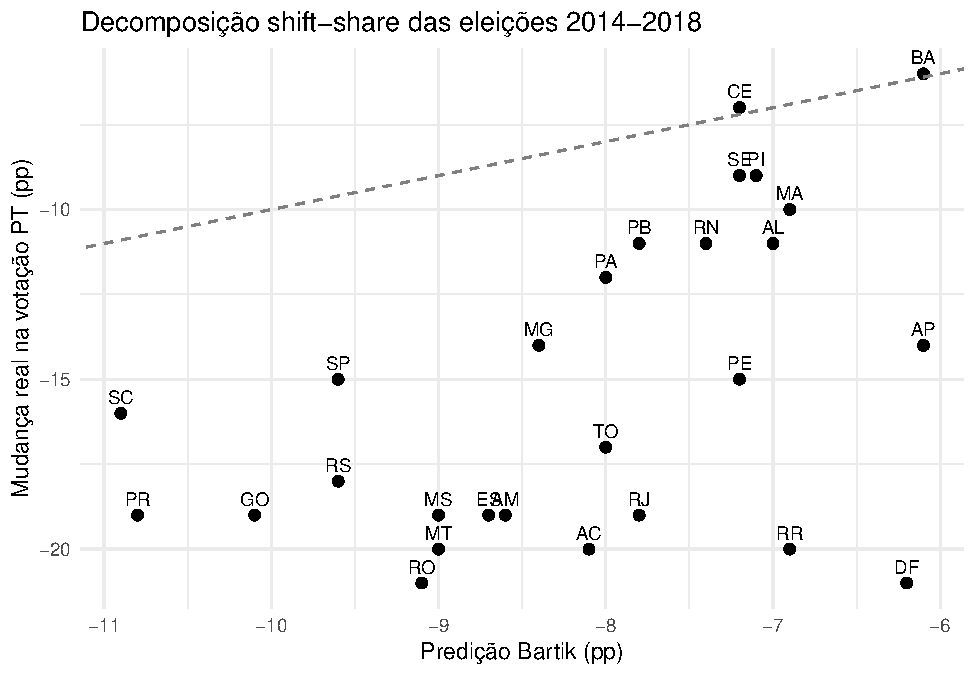
\includegraphics[keepaspectratio,alt={\label{fig:eleicoes-grafico}Mudan\textless U+00E7\textgreater a na vota\textless U+00E7\textgreater\textless U+00E3\textgreater o do PT (2014\textless U+2192\textgreater2018): observada vs.~predi\textless U+00E7\textgreater\textless U+00E3\textgreater o Bartik}]{bookdownproj_files/figure-latex/eleicoes-grafico-1.pdf}}
\caption{\label{fig:eleicoes-grafico}Mudan\textless U+00E7\textgreater a na vota\textless U+00E7\textgreater\textless U+00E3\textgreater o do PT (2014\textless U+2192\textgreater2018): observada vs.~predi\textless U+00E7\textgreater\textless U+00E3\textgreater o Bartik}
\end{figure}

O gráfico mostra que estados próximos à linha tracejada (45°) tiveram mudanças bem explicadas pela estrutura nacional; estados distantes da linha tiveram choques regionais importantes.

Agora aplicamos a decomposição completa nos três componentes A, B e C:

\begin{Shaded}
\begin{Highlighting}[]
\CommentTok{\# Shares em 2014 (t=0) e 2018 (t=1) — em fração}
\NormalTok{w\_0 }\OtherTok{\textless{}{-}}\NormalTok{ eleicoes[, }\FunctionTok{c}\NormalTok{(}\StringTok{"PT\_2014"}\NormalTok{,}\StringTok{"PSDB\_2014"}\NormalTok{,}\StringTok{"Outros\_2014"}\NormalTok{)] }\SpecialCharTok{/} \DecValTok{100}
\NormalTok{w\_t }\OtherTok{\textless{}{-}}\NormalTok{ eleicoes[, }\FunctionTok{c}\NormalTok{(}\StringTok{"PT\_2018"}\NormalTok{,}\StringTok{"PSDB\_2018"}\NormalTok{,}\StringTok{"Outros\_2018"}\NormalTok{)] }\SpecialCharTok{/} \DecValTok{100}

\CommentTok{\# D\_\{ijt\}: votação em 2018 (usamos os mesmos dados como proxy de intensidade)}
\NormalTok{D\_t }\OtherTok{\textless{}{-}}\NormalTok{ eleicoes[, }\FunctionTok{c}\NormalTok{(}\StringTok{"PT\_2018"}\NormalTok{,}\StringTok{"PSDB\_2018"}\NormalTok{,}\StringTok{"Outros\_2018"}\NormalTok{)]}

\CommentTok{\# Média nacional de D\_\{jt\} em 2018}
\NormalTok{D\_bar\_t }\OtherTok{\textless{}{-}} \FunctionTok{colMeans}\NormalTok{(D\_t)}

\CommentTok{\# Componente A: votação esperada = sum\_j w\_\{ij0\} * D\_bar\_\{jt\}}
\NormalTok{comp\_A }\OtherTok{\textless{}{-}} \FunctionTok{as.numeric}\NormalTok{(}\FunctionTok{as.matrix}\NormalTok{(w\_0) }\SpecialCharTok{\%*\%}\NormalTok{ D\_bar\_t)}

\CommentTok{\# Componente B: choque partidário = sum\_j w\_\{ij0\} * (D\_\{ijt\} {-} D\_bar\_\{jt\})}
\NormalTok{desvios }\OtherTok{\textless{}{-}} \FunctionTok{sweep}\NormalTok{(}\FunctionTok{as.matrix}\NormalTok{(D\_t), }\DecValTok{2}\NormalTok{, D\_bar\_t)}
\NormalTok{comp\_B }\OtherTok{\textless{}{-}} \FunctionTok{rowSums}\NormalTok{(}\FunctionTok{as.matrix}\NormalTok{(w\_0) }\SpecialCharTok{*}\NormalTok{ desvios)}

\CommentTok{\# Componente C: choque temporal = sum\_j (w\_\{ijt\} {-} w\_\{ij0\}) * D\_\{ijt\}}
\NormalTok{delta\_w }\OtherTok{\textless{}{-}} \FunctionTok{as.matrix}\NormalTok{(w\_t) }\SpecialCharTok{{-}} \FunctionTok{as.matrix}\NormalTok{(w\_0)}
\NormalTok{comp\_C }\OtherTok{\textless{}{-}} \FunctionTok{rowSums}\NormalTok{(delta\_w }\SpecialCharTok{*} \FunctionTok{as.matrix}\NormalTok{(D\_t))}

\NormalTok{temporal }\OtherTok{\textless{}{-}} \FunctionTok{data.frame}\NormalTok{(}
  \AttributeTok{UF =}\NormalTok{ eleicoes}\SpecialCharTok{$}\NormalTok{UF,}
  \AttributeTok{A\_esperado =} \FunctionTok{round}\NormalTok{(comp\_A, }\DecValTok{1}\NormalTok{),}
  \AttributeTok{B\_choque\_part =} \FunctionTok{round}\NormalTok{(comp\_B, }\DecValTok{1}\NormalTok{),}
  \AttributeTok{C\_choque\_temp =} \FunctionTok{round}\NormalTok{(comp\_C, }\DecValTok{1}\NormalTok{)}
\NormalTok{)}

\CommentTok{\# Tabela para estados selecionados}
\NormalTok{tab\_temp }\OtherTok{\textless{}{-}}\NormalTok{ temporal[temporal}\SpecialCharTok{$}\NormalTok{UF }\SpecialCharTok{\%in\%}\NormalTok{ estados\_sel, ]}
\NormalTok{tab\_temp }\OtherTok{\textless{}{-}}\NormalTok{ tab\_temp[}\FunctionTok{match}\NormalTok{(estados\_sel, tab\_temp}\SpecialCharTok{$}\NormalTok{UF), ]}

\FunctionTok{kable}\NormalTok{(tab\_temp, }\AttributeTok{row.names =} \ConstantTok{FALSE}\NormalTok{,}
      \AttributeTok{caption =} \StringTok{"Decomposição temporal A, B, C — estados selecionados"}\NormalTok{,}
      \AttributeTok{col.names =} \FunctionTok{c}\NormalTok{(}\StringTok{"UF"}\NormalTok{, }\StringTok{"A: esperado"}\NormalTok{, }\StringTok{"B: choque partidário"}\NormalTok{, }\StringTok{"C: choque temporal"}\NormalTok{))}
\end{Highlighting}
\end{Shaded}

\begin{table}

\caption{\label{tab:temporal-decomposicao}Decomposição temporal A, B, C — estados selecionados}
\centering
\begin{tabular}[t]{l|r|r|r}
\hline
UF & A: esperado & B: choque partidário & C: choque temporal\\
\hline
SP & 25.1 & -1.0 & 36.9\\
\hline
RJ & 28.2 & -2.3 & 33.5\\
\hline
MG & 29.1 & 0.2 & 18.1\\
\hline
BA & 34.6 & 12.6 & 3.4\\
\hline
CE & 32.8 & 9.4 & 5.7\\
\hline
RS & 26.2 & -2.3 & 36.3\\
\hline
PR & 24.5 & -1.9 & 40.9\\
\hline
PA & 31.1 & 3.9 & 11.5\\
\hline
PE & 32.8 & 5.9 & 8.4\\
\hline
MT & 26.5 & -2.8 & 41.5\\
\hline
\end{tabular}
\end{table}

\begin{Shaded}
\begin{Highlighting}[]
\FunctionTok{library}\NormalTok{(tidyr)}

\CommentTok{\# Preparar dados para gráfico de barras (estados selecionados)}
\NormalTok{plot\_data }\OtherTok{\textless{}{-}}\NormalTok{ temporal[temporal}\SpecialCharTok{$}\NormalTok{UF }\SpecialCharTok{\%in\%}\NormalTok{ estados\_sel, ]}
\NormalTok{plot\_data }\OtherTok{\textless{}{-}}\NormalTok{ plot\_data[}\FunctionTok{match}\NormalTok{(estados\_sel, plot\_data}\SpecialCharTok{$}\NormalTok{UF), ]}

\NormalTok{plot\_long }\OtherTok{\textless{}{-}} \FunctionTok{pivot\_longer}\NormalTok{(plot\_data, }\AttributeTok{cols =} \SpecialCharTok{{-}}\NormalTok{UF,}
                          \AttributeTok{names\_to =} \StringTok{"Componente"}\NormalTok{, }\AttributeTok{values\_to =} \StringTok{"Valor"}\NormalTok{)}
\NormalTok{plot\_long}\SpecialCharTok{$}\NormalTok{Componente }\OtherTok{\textless{}{-}} \FunctionTok{factor}\NormalTok{(plot\_long}\SpecialCharTok{$}\NormalTok{Componente,}
  \AttributeTok{levels =} \FunctionTok{c}\NormalTok{(}\StringTok{"A\_esperado"}\NormalTok{,}\StringTok{"B\_choque\_part"}\NormalTok{,}\StringTok{"C\_choque\_temp"}\NormalTok{),}
  \AttributeTok{labels =} \FunctionTok{c}\NormalTok{(}\StringTok{"A: Votação esperada"}\NormalTok{,}\StringTok{"B: Choque partidário"}\NormalTok{,}\StringTok{"C: Choque temporal"}\NormalTok{))}

\FunctionTok{ggplot}\NormalTok{(plot\_long, }\FunctionTok{aes}\NormalTok{(}\AttributeTok{x =}\NormalTok{ UF, }\AttributeTok{y =}\NormalTok{ Valor, }\AttributeTok{fill =}\NormalTok{ Componente)) }\SpecialCharTok{+}
  \FunctionTok{geom\_col}\NormalTok{(}\AttributeTok{position =} \StringTok{"dodge"}\NormalTok{) }\SpecialCharTok{+}
  \FunctionTok{labs}\NormalTok{(}\AttributeTok{x =} \StringTok{"Estado"}\NormalTok{, }\AttributeTok{y =} \StringTok{"Valor do componente"}\NormalTok{,}
       \AttributeTok{title =} \StringTok{"Decomposição shift{-}share das eleições 2018"}\NormalTok{,}
       \AttributeTok{fill =} \StringTok{"Componente"}\NormalTok{) }\SpecialCharTok{+}
  \FunctionTok{scale\_fill\_manual}\NormalTok{(}\AttributeTok{values =} \FunctionTok{c}\NormalTok{(}\StringTok{"orange"}\NormalTok{,}\StringTok{"purple"}\NormalTok{,}\StringTok{"\#008080"}\NormalTok{)) }\SpecialCharTok{+}
  \FunctionTok{theme\_minimal}\NormalTok{() }\SpecialCharTok{+}
  \FunctionTok{theme}\NormalTok{(}\AttributeTok{axis.text.x =} \FunctionTok{element\_text}\NormalTok{(}\AttributeTok{angle =} \DecValTok{0}\NormalTok{))}
\end{Highlighting}
\end{Shaded}

\begin{figure}
\centering
\pandocbounded{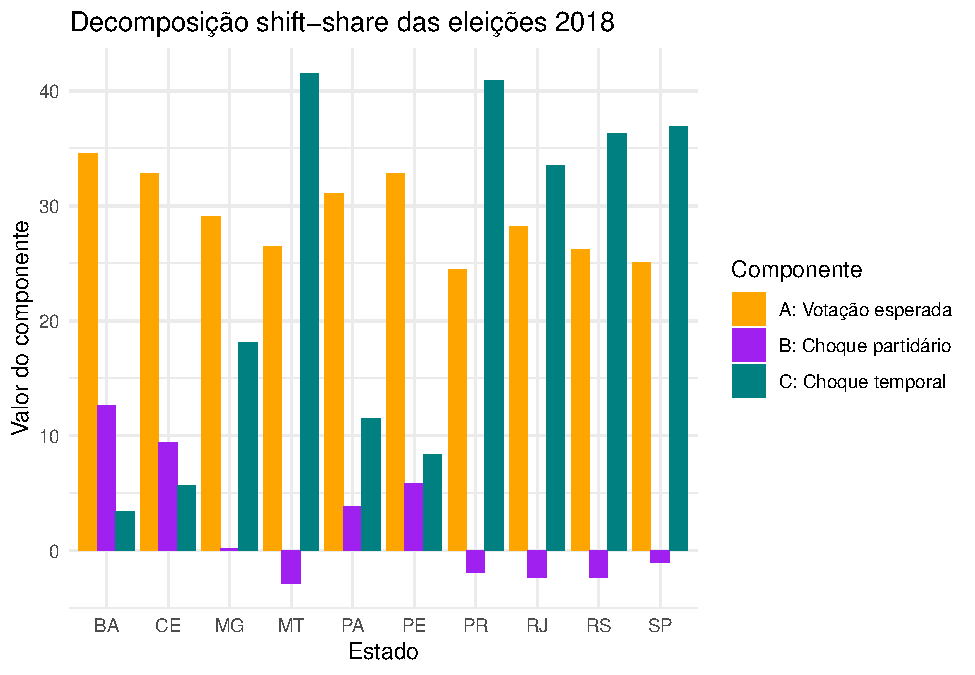
\includegraphics[keepaspectratio,alt={\label{fig:temporal-grafico}Componentes shift-share da vota\textless U+00E7\textgreater\textless U+00E3\textgreater o 2018 por estado}]{bookdownproj_files/figure-latex/temporal-grafico-1.pdf}}
\caption{\label{fig:temporal-grafico}Componentes shift-share da vota\textless U+00E7\textgreater\textless U+00E3\textgreater o 2018 por estado}
\end{figure}

O gráfico ilustra como o resultado eleitoral de 2018 em cada estado se decompõe nos três componentes. O componente A (votação esperada) é relativamente estável; as maiores diferenças entre estados vêm dos componentes B (choque partidário --- refletindo o colapso diferencial do PSDB e a ascensão de Bolsonaro) e C (choque temporal --- refletindo realinhamentos regionais como a resistência do PT no Nordeste).

\subsection{O instrumento shift-share como variável instrumental}\label{o-instrumento-shift-share-como-variuxe1vel-instrumental}

A decomposição acima é útil descritivamente, mas o verdadeiro poder do shift-share está no seu uso como variável instrumental. Vamos formalizar a construção e entender as condições de identificação.

\subsubsection{Construção formal}\label{construuxe7uxe3o-formal}

Considere \(N\) estados (indexados por \(i\)) e \(K\) partidos (indexados por \(k\)). Para cada estado \(i\), observamos a parcela (\emph{share}) de votos do partido \(k\) em um período-base \(t_0\):

\begin{equation}
w_{ik} = \frac{V_{ik,t_0}}{V_{i,t_0}}
\label{eq:share-def}
\end{equation}

onde \(V_{ik,t_0}\) é o total de votos no partido \(k\) no estado \(i\) no período-base, e \(V_{i,t_0}\) é o total de votos válidos no estado \(i\). Note que \(\sum_k w_{ik} = 1\).

Observamos também um choque (\emph{shift}) agregado no nível do partido \(k\), denotado \(g_k\). Por exemplo, \(g_k\) pode ser a variação nacional na votação do partido \(k\):

\begin{equation}
g_k = \frac{\Delta V_k^{\text{Nacional}}}{V_{k,t_0}^{\text{Nacional}}}
\label{eq:shift-def}
\end{equation}

O \textbf{instrumento shift-share} (ou instrumento Bartik) para o estado \(i\) é definido como:

\begin{equation}
B_i = \sum_{k=1}^{K} w_{ik} \cdot g_k
\label{eq:bartik}
\end{equation}

Este instrumento calcula a média ponderada dos choques partidários nacionais, usando as \emph{shares} pré-determinadas como pesos. A intuição é que estados com composição partidária diferente serão diferencialmente afetados pelas mesmas tendências nacionais. Por exemplo, um estado com alta concentração inicial de votos no PT será mais afetado por uma queda nacional do PT do que um estado onde o PT era minoritário.

Embora aqui ilustremos com votos e partidos, a mesma lógica se aplica a setores econômicos e emprego (a aplicação clássica de Bartik 1991), a parceiros comerciais e comércio, ou a qualquer variável decomponível em subunidades excludentes.

\subsubsection{\texorpdfstring{Voltando ao exemplo: construindo \(w_{ik}\), \(g_k\) e \(B_i\) com dados eleitorais}{Voltando ao exemplo: construindo w\_\{ik\}, g\_k e B\_i com dados eleitorais}}\label{voltando-ao-exemplo-construindo-w_ik-g_k-e-b_i-com-dados-eleitorais}

Podemos agora mapear cada elemento da construção formal nos dados das eleições 2014→2018 já analisados. Nossos ``setores'' (\(k\)) são os três blocos partidários (PT, PSDB, Outros) e nossas ``regiões'' (\(i\)) são os 27 estados.

As \textbf{shares} \(w_{ik}\) são a composição partidária de cada estado em 2014 (o período-base \(t_0\)):

\begin{Shaded}
\begin{Highlighting}[]
\CommentTok{\# w\_\{ik\} = fração de votos do partido k no estado i em 2014}
\NormalTok{tab\_shares }\OtherTok{\textless{}{-}} \FunctionTok{data.frame}\NormalTok{(}
  \AttributeTok{UF =}\NormalTok{ eleicoes}\SpecialCharTok{$}\NormalTok{UF,}
  \AttributeTok{w\_PT =} \FunctionTok{round}\NormalTok{(shares\_2014}\SpecialCharTok{$}\NormalTok{PT\_2014, }\DecValTok{2}\NormalTok{),}
  \AttributeTok{w\_PSDB =} \FunctionTok{round}\NormalTok{(shares\_2014}\SpecialCharTok{$}\NormalTok{PSDB\_2014, }\DecValTok{2}\NormalTok{),}
  \AttributeTok{w\_Outros =} \FunctionTok{round}\NormalTok{(shares\_2014}\SpecialCharTok{$}\NormalTok{Outros\_2014, }\DecValTok{2}\NormalTok{)}
\NormalTok{)}

\NormalTok{tab\_shares\_sel }\OtherTok{\textless{}{-}}\NormalTok{ tab\_shares[tab\_shares}\SpecialCharTok{$}\NormalTok{UF }\SpecialCharTok{\%in\%} \FunctionTok{c}\NormalTok{(}\StringTok{"BA"}\NormalTok{,}\StringTok{"CE"}\NormalTok{,}\StringTok{"MG"}\NormalTok{,}\StringTok{"SP"}\NormalTok{,}\StringTok{"RS"}\NormalTok{), ]}
\NormalTok{tab\_shares\_sel }\OtherTok{\textless{}{-}}\NormalTok{ tab\_shares\_sel[}\FunctionTok{match}\NormalTok{(}\FunctionTok{c}\NormalTok{(}\StringTok{"BA"}\NormalTok{,}\StringTok{"CE"}\NormalTok{,}\StringTok{"MG"}\NormalTok{,}\StringTok{"SP"}\NormalTok{,}\StringTok{"RS"}\NormalTok{), tab\_shares\_sel}\SpecialCharTok{$}\NormalTok{UF), ]}
\FunctionTok{kable}\NormalTok{(tab\_shares\_sel, }\AttributeTok{row.names =} \ConstantTok{FALSE}\NormalTok{,}
      \AttributeTok{caption =} \StringTok{"Shares $w\_\{ik\}$: composição partidária em 2014 (fração dos votos válidos)"}\NormalTok{,}
      \AttributeTok{col.names =} \FunctionTok{c}\NormalTok{(}\StringTok{"Estado (i)"}\NormalTok{, }\StringTok{"$w\_\{i,PT\}$"}\NormalTok{, }\StringTok{"$w\_\{i,PSDB\}$"}\NormalTok{, }\StringTok{"$w\_\{i,Outros\}$"}\NormalTok{))}
\end{Highlighting}
\end{Shaded}

\begin{table}

\caption{\label{tab:ss-iv-shares}Shares $w_{ik}$: composição partidária em 2014 (fração dos votos válidos)}
\centering
\begin{tabular}[t]{l|r|r|r}
\hline
Estado (i) & \$w\_\{i,PT\}\$ & \$w\_\{i,PSDB\}\$ & \$w\_\{i,Outros\}\$\\
\hline
BA & 0.66 & 0.15 & 0.19\\
\hline
CE & 0.62 & 0.20 & 0.18\\
\hline
MG & 0.47 & 0.34 & 0.19\\
\hline
SP & 0.31 & 0.49 & 0.20\\
\hline
RS & 0.37 & 0.44 & 0.19\\
\hline
\end{tabular}
\end{table}

A Bahia tem \(w_{BA,PT} = 0{,}66\): dois terços dos votos foram para o PT em 2014. Já São Paulo tem \(w_{SP,PT} = 0{,}31\). Essa diferença na composição inicial é o que gera variação no instrumento.

Os \textbf{shifts} \(g_k\) são as mudanças nacionais na votação de cada bloco entre 2014 e 2018:

\begin{Shaded}
\begin{Highlighting}[]
\NormalTok{tab\_shifts }\OtherTok{\textless{}{-}} \FunctionTok{data.frame}\NormalTok{(}
  \AttributeTok{Partido =} \FunctionTok{c}\NormalTok{(}\StringTok{"PT"}\NormalTok{, }\StringTok{"PSDB"}\NormalTok{, }\StringTok{"Outros"}\NormalTok{),}
  \AttributeTok{g\_k =} \FunctionTok{round}\NormalTok{(shifts }\SpecialCharTok{*} \DecValTok{100}\NormalTok{, }\DecValTok{1}\NormalTok{)}
\NormalTok{)}
\FunctionTok{kable}\NormalTok{(tab\_shifts, }\AttributeTok{row.names =} \ConstantTok{FALSE}\NormalTok{,}
      \AttributeTok{caption =} \StringTok{"Shifts $g\_k$: mudança nacional na votação de cada bloco (pp)"}\NormalTok{,}
      \AttributeTok{col.names =} \FunctionTok{c}\NormalTok{(}\StringTok{"Partido ($k$)"}\NormalTok{, }\StringTok{"$g\_k$ (pp)"}\NormalTok{))}
\end{Highlighting}
\end{Shaded}

\begin{table}

\caption{\label{tab:ss-iv-shifts}Shifts $g_k$: mudança nacional na votação de cada bloco (pp)}
\centering
\begin{tabular}[t]{l|r}
\hline
Partido (\$k\$) & \$g\_k\$ (pp)\\
\hline
PT & -15.2\\
\hline
PSDB & -27.4\\
\hline
Outros & 42.6\\
\hline
\end{tabular}
\end{table}

O PT caiu cerca de 16pp nacionalmente, o PSDB desmoronou \textasciitilde26pp, e o bloco Outros (liderado por Bolsonaro e Ciro) subiu \textasciitilde43pp. Esses choques são os mesmos para todos os estados --- são tendências \textbf{nacionais}.

Finalmente, o \textbf{instrumento Bartik} \(B_i = \sum_k w_{ik} \cdot g_k\) combina as shares iniciais com os shifts nacionais:

\begin{Shaded}
\begin{Highlighting}[]
\NormalTok{tab\_bartik }\OtherTok{\textless{}{-}} \FunctionTok{data.frame}\NormalTok{(}
  \AttributeTok{UF =}\NormalTok{ eleicoes}\SpecialCharTok{$}\NormalTok{UF,}
  \AttributeTok{Bartik =} \FunctionTok{round}\NormalTok{(bartik }\SpecialCharTok{*} \DecValTok{100}\NormalTok{, }\DecValTok{1}\NormalTok{)}
\NormalTok{)}
\NormalTok{tab\_bartik\_sel }\OtherTok{\textless{}{-}}\NormalTok{ tab\_bartik[tab\_bartik}\SpecialCharTok{$}\NormalTok{UF }\SpecialCharTok{\%in\%} \FunctionTok{c}\NormalTok{(}\StringTok{"BA"}\NormalTok{,}\StringTok{"CE"}\NormalTok{,}\StringTok{"MG"}\NormalTok{,}\StringTok{"SP"}\NormalTok{,}\StringTok{"RS"}\NormalTok{), ]}
\NormalTok{tab\_bartik\_sel }\OtherTok{\textless{}{-}}\NormalTok{ tab\_bartik\_sel[}\FunctionTok{match}\NormalTok{(}\FunctionTok{c}\NormalTok{(}\StringTok{"BA"}\NormalTok{,}\StringTok{"CE"}\NormalTok{,}\StringTok{"MG"}\NormalTok{,}\StringTok{"SP"}\NormalTok{,}\StringTok{"RS"}\NormalTok{), tab\_bartik\_sel}\SpecialCharTok{$}\NormalTok{UF), ]}
\FunctionTok{kable}\NormalTok{(tab\_bartik\_sel, }\AttributeTok{row.names =} \ConstantTok{FALSE}\NormalTok{,}
      \AttributeTok{caption =} \StringTok{"Instrumento Bartik $B\_i$ para cada estado (pp)"}\NormalTok{,}
      \AttributeTok{col.names =} \FunctionTok{c}\NormalTok{(}\StringTok{"Estado ($i$)"}\NormalTok{, }\StringTok{"$B\_i$ (pp)"}\NormalTok{))}
\end{Highlighting}
\end{Shaded}

\begin{table}

\caption{\label{tab:ss-iv-bartik}Instrumento Bartik $B_i$ para cada estado (pp)}
\centering
\begin{tabular}[t]{l|r}
\hline
Estado (\$i\$) & \$B\_i\$ (pp)\\
\hline
BA & -6.1\\
\hline
CE & -7.2\\
\hline
MG & -8.4\\
\hline
SP & -9.6\\
\hline
RS & -9.6\\
\hline
\end{tabular}
\end{table}

Observe que \textbf{os shifts \(g_k\) são idênticos para todos os estados} --- o que diferencia os \(B_i\) entre si são exclusivamente as shares \(w_{ik}\). A Bahia, com 66\% de votos no PT em 2014, é muito mais exposta à queda nacional do PT do que São Paulo, com 31\%. É essa variação \emph{cross-sectional} no instrumento, gerada pela composição inicial, que permite a identificação.

\subsubsection{O modelo estrutural e o IV}\label{o-modelo-estrutural-e-o-iv}

O objetivo típico é estimar o efeito causal de uma variável endógena \(X_i\) sobre uma variável de resultado \(Y_i\). O modelo estrutural é:

\begin{equation}
Y_i = \alpha + \beta X_i + \varepsilon_i
\label{eq:estrutural-shift-share}
\end{equation}

onde \(X_i\) é endógena (por exemplo, crescimento do emprego local ou mudança na votação, que é tanto causa quanto consequência de outros fatores locais). OLS é inconsistente porque \(\text{Cov}(X_i, \varepsilon_i) \neq 0\).

\textbf{Primeiro estágio (\emph{first stage})}: O instrumento \(B_i\) prevê \(X_i\):

\begin{equation}
X_i = \gamma_0 + \gamma_1 B_i + \nu_i
\label{eq:first-stage}
\end{equation}

A condição de relevância exige \(\gamma_1 \neq 0\): as \emph{shares} combinadas com os \emph{shifts} devem efetivamente prever a variável endógena.

\textbf{Segundo estágio (\emph{second stage})}: Substitui-se \(X_i\) por \(\hat{X}_i\):

\begin{equation}
Y_i = \alpha + \beta \hat{X}_i + \eta_i
\label{eq:second-stage}
\end{equation}

A condição de exclusão exige \(\text{Cov}(B_i, \varepsilon_i) = 0\): o instrumento só afeta \(Y_i\) através de \(X_i\).

\subsubsection{Interpretando o modelo com o exemplo eleitoral}\label{interpretando-o-modelo-com-o-exemplo-eleitoral}

Vamos dar concretude ao modelo acima usando nosso exemplo. Suponha que queremos estimar o efeito causal da \textbf{mudança na votação do PT} (\(X_i\) = queda do PT em pp no estado \(i\)) sobre alguma variável de resultado político \(Y_i\) --- por exemplo, o nível de abstenção, o gasto público municipal ou a ocorrência de protestos.

O problema é que a queda do PT em cada estado não é aleatória: ela está correlacionada com fatores locais não observados (\(U_i\)), como a força de lideranças locais, o nível de desemprego estadual, a cobertura midiática da Lava-Jato, entre outros. Esses mesmos fatores podem afetar \(Y_i\) diretamente. Por isso, OLS é inconsistente.

\textbf{Primeiro estágio}: O instrumento Bartik \(B_i\) prevê a queda do PT no estado \(i\). A lógica é que estados com maior concentração inicial de votos no PT (\(w_{i,PT}\) alto) estão mecanicamente mais expostos à tendência nacional de queda do PT. O primeiro estágio estima:

\[X_i = \gamma_0 + \gamma_1 B_i + \nu_i\]

Se \(\gamma_1\) é significativamente diferente de zero, o instrumento é \textbf{relevante} --- as tendências nacionais, filtradas pela composição inicial, efetivamente preveem a mudança local. No nosso exemplo, o gráfico da seção anterior (mudança real vs.~predição Bartik) já mostrou que essa relação é forte: estados onde o Bartik prevê queda maior de fato tiveram queda maior.

\textbf{Segundo estágio}: Substituímos \(X_i\) por seu valor predito \(\hat{X}_i\) --- a parte da mudança local que é explicada \emph{apenas} pelas tendências nacionais interagidas com a composição inicial:

\[Y_i = \alpha + \beta \hat{X}_i + \eta_i\]

A estimativa \(\hat{\beta}\) captura o efeito causal de \(X_i\) sobre \(Y_i\), \textbf{desde que o instrumento satisfaça a restrição de exclusão}. Intuitivamente, ao usar \(\hat{X}_i\) em vez de \(X_i\), estamos ``limpando'' a variação endógena (fatores locais) e ficando apenas com a variação exógena (exposição a tendências nacionais via composição inicial).

\subsubsection{Por que o instrumento seria válido? Uma discussão intuitiva}\label{por-que-o-instrumento-seria-vuxe1lido-uma-discussuxe3o-intuitiva}

Podemos visualizar a estrutura causal do instrumento shift-share com um DAG:

\begin{figure}
\centering
\pandocbounded{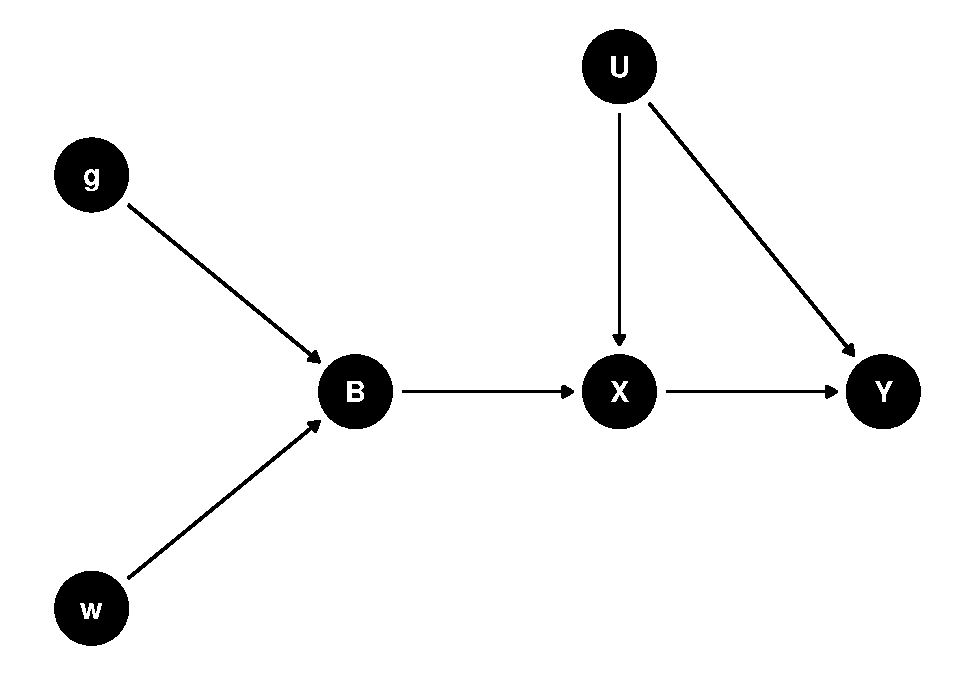
\includegraphics[keepaspectratio,alt={\label{fig:dag-ss}DAG do instrumento shift-share. O instrumento B\_i \textless U+00E9\textgreater{} constru\textless U+00ED\textgreater do a partir das shares iniciais (w) e dos choques nacionais (g). A restri\textless U+00E7\textgreater\textless U+00E3\textgreater o de exclus\textless U+00E3\textgreater o exige que n\textless U+00E3\textgreater o haja caminho direto de B para Y que n\textless U+00E3\textgreater o passe por X.}]{bookdownproj_files/figure-latex/dag-ss-1.pdf}}
\caption{\label{fig:dag-ss}DAG do instrumento shift-share. O instrumento \(B_i\) \textless U+00E9\textgreater{} constru\textless U+00ED\textgreater do a partir das shares iniciais (\(w\)) e dos choques nacionais (\(g\)). A restri\textless U+00E7\textgreater\textless U+00E3\textgreater o de exclus\textless U+00E3\textgreater o exige que n\textless U+00E3\textgreater o haja caminho direto de \(B\) para \(Y\) que n\textless U+00E3\textgreater o passe por \(X\).}
\end{figure}

No DAG acima, \(g\) representa os choques nacionais (\(g_k\)), \(w\) as shares iniciais (\(w_{ik}\)), \(B\) o instrumento Bartik (\(B_i\)), \(X\) a variável endógena (\(X_i\)), \(U\) os confundidores não observados (\(U_i\)) e \(Y\) o resultado (\(Y_i\)). O confundidor \(U\) cria um \emph{backdoor} entre \(X\) e \(Y\), tornando OLS inconsistente. O instrumento \(B\) é válido se o \textbf{único caminho} de \(B\) para \(Y\) passa por \(X\).

A \textbf{restrição de exclusão} seria violada se houvesse uma seta direta de \(B\) para \(Y\) (ou, equivalentemente, de \(w\) ou \(g\) para \(Y\) por canais que não passam por \(X\)). No nosso exemplo eleitoral, isso aconteceria se:

\begin{itemize}
\item
  A \textbf{composição partidária inicial} (\(w_{ik}\)) afetasse \(Y_i\) diretamente. Por exemplo, se estados mais ``petistas'' em 2014 fossem sistematicamente mais pobres ou mais urbanizados, e essas características afetassem \(Y_i\) (abstenção, protestos etc.) por canais que não passam pela mudança na votação do PT, o instrumento seria inválido.
\item
  Os \textbf{choques nacionais} (\(g_k\)) refletissem fatores que também afetassem \(Y_i\) diretamente. Por exemplo, se a Lava-Jato afetasse tanto os votos (via \(X_i\)) quanto os protestos (via um canal direto), a restrição seria violada.
\end{itemize}

É importante reconhecer que o nosso exemplo hipotético de IV --- usar a mudança eleitoral como instrumento para algum outcome estadual como abstenção, gasto público ou protestos --- enfrenta desafios reais de identificação. Primeiro, com \(N = 27\) estados, o número de observações é muito pequeno para estimação IV confiável (instrumentos fracos, inferência imprecisa). Segundo, as \emph{shares} e os \emph{shifts} operam no \textbf{mesmo nível geográfico} que o outcome: tendências nacionais por partido afetam os estados, e os outcomes também são estaduais, dificultando a separação entre o canal causal de interesse e outros canais. Terceiro, fatores como a mudança de governador entre 2014 e 2018 são parte do próprio mecanismo político que liga tendências nacionais a resultados locais, confundindo o canal causal.

Uma solução para esses problemas é explorar \textbf{variação cross-level} --- usar choques de um nível geográfico (por exemplo, tendências estaduais) para prever outcomes em outro nível (por exemplo, municipal). Quando os \emph{shifts} são computados em um nível mais agregado do que a unidade de observação, a separação entre instrumento e confundidores locais se torna mais plausível. Além disso, o \textbf{leave-out design} --- excluir a própria unidade ao computar o \emph{shift} agregado --- elimina a correlação mecânica entre o instrumento e choques locais não observados.

Xu (2025, \emph{Journal of Politics}) oferece um exemplo concreto e bem-sucedido de como resolver esses problemas em uma aplicação de SSIV na ciência política brasileira, usando variação cross-level entre eleições estaduais e outcomes municipais combinada com um leave-out design. Discutimos esse estudo em detalhe na seção de aplicações em ciência política.

A questão crucial que emerge é: \textbf{de onde, exatamente, vem a exogeneidade do instrumento?} Das \emph{shares}? Dos \emph{shifts}? De ambos? Essa pergunta tem duas respostas formais distintas, que correspondem a duas estratégias de identificação com implicações muito diferentes para diagnósticos e credibilidade. É exatamente isso que a próxima seção formaliza.

\subsection{Duas estratégias de identificação}\label{duas-estratuxe9gias-de-identificauxe7uxe3o}

Uma revolução metodológica recente (2018-2025) esclareceu que há duas maneiras distintas de justificar a exogeneidade do instrumento shift-share. A referência pedagógica central é Borusyak, Hull \& Jaravel (2025), publicada no \emph{Journal of Economic Perspectives}.

\subsubsection{Estratégia 1: Exogeneidade das shares (GPSS 2020)}\label{estratuxe9gia-1-exogeneidade-das-shares-gpss-2020}

Goldsmith-Pinkham, Sorkin \& Swift (2020) demonstram um resultado de equivalência fundamental. Para entender essa equivalência, é útil primeiro ter uma intuição sobre GMM (Método Generalizado dos Momentos).

\textbf{Intuição sobre GMM.} O estimador de MQO (OLS) pode ser entendido como a solução de uma condição de momento: encontrar \(\beta\) tal que \(\mathbb{E}[X_i' \varepsilon_i] = 0\), ou seja, os resíduos são não correlacionados com os regressores. Quando temos instrumentos \(Z_i\), o estimador de IV impõe a condição \(\mathbb{E}[Z_i' \varepsilon_i] = 0\). Quando há exatamente tantos instrumentos quanto variáveis endógenas (identificação exata), existe uma única solução. Mas quando há \emph{mais} instrumentos que variáveis endógenas --- o caso de \textbf{sobreidentificação} --- o sistema tem mais equações que incógnitas, e em geral não existe \(\beta\) que satisfaça todas as condições simultaneamente. O GMM resolve esse problema encontrando o \(\beta\) que melhor satisfaz todas as condições de momento ao mesmo tempo, atribuindo pesos ótimos a cada condição. No caso shift-share, cada \emph{share} \(w_{ik}\) (para \(k = 1, ..., K\)) pode ser vista como um instrumento separado, gerando \(K\) condições de momento --- uma situação típica de sobreidentificação.

A equivalência demonstrada por GPSS é que o estimador IV usando \(B_i = \sum_k w_{ik} g_k\) como instrumento único é \textbf{numericamente idêntico} a um estimador GMM que usa cada \emph{share} \(w_{ik}\) como instrumento separado, com os \emph{shifts} \(g_k\) servindo apenas como pesos na combinação ótima:

\begin{equation}
\hat{\beta}^{IV} = \sum_k \hat{\alpha}_k \hat{\beta}_k
\label{eq:gpss-equiv}
\end{equation}

onde \(\hat{\beta}_k\) é a estimativa \emph{just-identified} usando apenas \(w_{ik}\) como instrumento (para o partido \(k\)), e \(\hat{\alpha}_k\) é o \textbf{peso de Rotemberg} que mede a influência relativa do partido \(k\) na estimativa global. Os pesos de Rotemberg satisfazem \(\sum_k \hat{\alpha}_k = 1\) mas podem ser \textbf{negativos}, o que é um sinal de alerta.

Em outras palavras: usar o instrumento Bartik \(B_i\) é matematicamente equivalente a usar todas as \(K\) \emph{shares} como instrumentos separados via GMM. A escolha entre os dois é uma questão de conveniência, não de substância.

\textbf{Hipótese de identificação}: As \emph{shares} iniciais \(w_{ik}\) são exógenas --- isto é, não correlacionadas com fatores não observados que afetam \(Y_i\):

\begin{equation}
\mathbb{E}[w_{ik} \cdot \varepsilon_i] = 0 \quad \forall k
\label{eq:gpss-id}
\end{equation}

Os \emph{shifts} \(g_k\) não precisam ser exógenos; eles apenas afetam a ponderação e a relevância do instrumento.

\textbf{Diagnósticos}: Calcular os Rotemberg weights \(\hat{\alpha}_k\) para identificar quais partidos (ou setores) mais influenciam a estimativa. Testar balanceamento das \emph{shares} mais influentes contra covariáveis pré-determinadas.

\subsubsection{Estratégia 2: Exogeneidade dos shifts (BHJ 2022)}\label{estratuxe9gia-2-exogeneidade-dos-shifts-bhj-2022}

Borusyak, Hull \& Jaravel (2022) oferecem um \emph{framework} alternativo. A regressão IV no nível regional é numericamente equivalente a uma regressão IV no \textbf{nível do choque} (partido/setor), onde a variável de resultado e o tratamento são agregados ao nível do choque usando as \emph{shares} como pesos:

\begin{equation}
\bar{Y}_k = \sum_i s_{ik} Y_i, \quad \bar{X}_k = \sum_i s_{ik} X_i
\label{eq:bhj-agreg}
\end{equation}

onde \(s_{ik} = w_{ik} / \sum_i w_{ik}\) normaliza os pesos. A regressão no nível do choque:

\begin{equation}
\bar{Y}_k = \alpha + \beta \bar{X}_k + \bar{\varepsilon}_k
\label{eq:bhj-reg}
\end{equation}

instrumentada por \(g_k\), produz \textbf{exatamente a mesma estimativa} \(\hat{\beta}\) que a regressão regional com \(B_i\).

\textbf{Hipótese de identificação}: Os choques \(g_k\) são quase aleatoriamente atribuídos --- isto é, não correlacionados com a média ponderada (por \emph{shares}) dos fatores não observados regionais:

\begin{equation}
\mathbb{E}[g_k \cdot \bar{\varepsilon}_k] = 0 \quad \forall k
\label{eq:bhj-id}
\end{equation}

As \emph{shares} \(w_{ik}\) podem ser endógenas. A identificação vem inteiramente da aleatoriedade dos choques, dado que há muitos choques independentes (\(K \to \infty\)).

\textbf{Diagnósticos}: Testes de pré-tendências e balanceamento no nível do choque. Verificar se \(g_k\) correlaciona-se com \(\bar{\varepsilon}_k\) pré-tratamento.

\subsubsection{Resumo das duas estratégias}\label{resumo-das-duas-estratuxe9gias}

\begin{longtable}[]{@{}
  >{\raggedright\arraybackslash}p{(\linewidth - 4\tabcolsep) * \real{0.3333}}
  >{\raggedright\arraybackslash}p{(\linewidth - 4\tabcolsep) * \real{0.3333}}
  >{\raggedright\arraybackslash}p{(\linewidth - 4\tabcolsep) * \real{0.3333}}@{}}
\toprule\noalign{}
\begin{minipage}[b]{\linewidth}\raggedright
\end{minipage} & \begin{minipage}[b]{\linewidth}\raggedright
\textbf{\emph{Shares} exógenas} (GPSS 2020)
\end{minipage} & \begin{minipage}[b]{\linewidth}\raggedright
\textbf{\emph{Shifts} exógenos} (BHJ 2022)
\end{minipage} \\
\midrule\noalign{}
\endhead
\bottomrule\noalign{}
\endlastfoot
\textbf{Hipótese-chave} & \(\mathbb{E}[w_{ik} \cdot \varepsilon_i] = 0\) & \(\mathbb{E}[g_k \cdot \bar{\varepsilon}_k] = 0\) \\
\textbf{\emph{Shares} podem ser endógenas?} & Não & Sim \\
\textbf{\emph{Shifts} podem ser endógenos?} & Sim (só afetam pesos) & Não \\
\textbf{N. de choques necessário} & Pode funcionar com poucos & Precisa de muitos (\(K\) grande) \\
\textbf{Diagnósticos} & Rotemberg weights, balanceamento nas \emph{shares} & Pré-tendências e balanceamento no nível do choque \\
\textbf{Aplicações típicas} & Elasticidades de oferta de trabalho, especialização histórica exógena & Imigração (enclave), comércio (China Shock) \\
\end{longtable}

\subsection{O problema de inferência}\label{o-problema-de-inferuxeancia}

Adão, Kolesár \& Morales (2019) identificam um problema crítico: erros-padrão convencionais (incluindo \emph{clustered} por região ou estado) são \textbf{severamente subestimados} em regressões shift-share. Em exercícios de placebo, testes ao nível nominal de 5\% rejeitam a hipótese nula verdadeira até \textbf{55\%} das vezes.

O problema surge porque resíduos \(\hat{\varepsilon}_i\) são correlacionados entre regiões com composição setorial similar, independentemente de proximidade geográfica. Duas regiões \(i\) e \(j\) com \emph{shares} parecidos (\(w_{ik} \approx w_{jk}\)) compartilham exposição aos mesmos choques setoriais, induzindo correlação em \(\hat{\varepsilon}_i\) e \(\hat{\varepsilon}_j\) que não é capturada por \emph{clustering} geográfico.

Na prática, os intervalos de confiança corrigidos por AKM são substancialmente mais largos que os convencionais.

\textbf{Alternativa BHJ}: Em vez de corrigir os erros-padrão no nível regional, rodar a regressão diretamente no nível do choque (via \texttt{ssaggregate}) e usar erros-padrão convencionais (heteroscedasticidade-robustos) no nível do choque. Se os choques são independentes, a inferência convencional é válida.

\subsection{Implementação em R}\label{implementauxe7uxe3o-em-r}

\subsubsection{Construção do instrumento}\label{construuxe7uxe3o-do-instrumento}

O instrumento \(B_i = \sum_k w_{ik} g_k\) é uma simples multiplicação matricial:

\begin{Shaded}
\begin{Highlighting}[]
\CommentTok{\# shares: matriz N x K de exposure shares (cada linha soma 1)}
\CommentTok{\# shocks: vetor K x 1 de choques setoriais}
\NormalTok{bartik\_instrument }\OtherTok{\textless{}{-}}\NormalTok{ shares }\SpecialCharTok{\%*\%}\NormalTok{ shocks}
\end{Highlighting}
\end{Shaded}

\subsubsection{Estimação IV}\label{estimauxe7uxe3o-iv}

Diversos pacotes R permitem estimar 2SLS. O \texttt{fixest} é recomendado por sua velocidade e suporte a efeitos fixos:

\begin{Shaded}
\begin{Highlighting}[]
\FunctionTok{library}\NormalTok{(fixest)}

\CommentTok{\# Construir instrumento}
\NormalTok{dados}\SpecialCharTok{$}\NormalTok{bartik }\OtherTok{\textless{}{-}} \FunctionTok{as.numeric}\NormalTok{(shares }\SpecialCharTok{\%*\%}\NormalTok{ shocks)}

\CommentTok{\# IV com efeitos fixos de estado}
\NormalTok{modelo }\OtherTok{\textless{}{-}} \FunctionTok{feols}\NormalTok{(y }\SpecialCharTok{\textasciitilde{}}\NormalTok{ controles }\SpecialCharTok{|}\NormalTok{ estado }\SpecialCharTok{|}\NormalTok{ x\_endogeno }\SpecialCharTok{\textasciitilde{}}\NormalTok{ bartik, }\AttributeTok{data =}\NormalTok{ dados)}
\FunctionTok{summary}\NormalTok{(modelo)}
\end{Highlighting}
\end{Shaded}

\subsubsection{\texorpdfstring{Erros-padrão corrigidos: pacote \texttt{ShiftShareSE}}{Erros-padrão corrigidos: pacote ShiftShareSE}}\label{erros-padruxe3o-corrigidos-pacote-shiftsharese}

O pacote \texttt{ShiftShareSE}, de Michal Kolesár, está disponível no CRAN e implementa os erros-padrão AKM (Adão, Kolesár \& Morales, 2019):

\begin{Shaded}
\begin{Highlighting}[]
\FunctionTok{install.packages}\NormalTok{(}\StringTok{"ShiftShareSE"}\NormalTok{)}
\FunctionTok{library}\NormalTok{(ShiftShareSE)}

\CommentTok{\# IV com SEs corrigidos para shift{-}share}
\NormalTok{resultado }\OtherTok{\textless{}{-}} \FunctionTok{ivreg\_ss}\NormalTok{(y }\SpecialCharTok{\textasciitilde{}}\NormalTok{ x\_endogeno }\SpecialCharTok{|}\NormalTok{ bartik,}
                       \AttributeTok{X =}\NormalTok{ shares\_matrix,    }\CommentTok{\# matriz N x K de shares}
                       \AttributeTok{data =}\NormalTok{ dados)}
\FunctionTok{summary}\NormalTok{(resultado)}
\end{Highlighting}
\end{Shaded}

Este pacote é essencial porque, como demonstrado por AKM, erros-padrão convencionais (mesmo clusterizados por geografia) são severamente subestimados em designs shift-share.

\subsubsection{\texorpdfstring{Agregação ao nível do choque: pacote \texttt{ssaggregate}}{Agregação ao nível do choque: pacote ssaggregate}}\label{agregauxe7uxe3o-ao-nuxedvel-do-choque-pacote-ssaggregate}

O pacote \texttt{ssaggregate}, de Kyle Butts, implementa a agregação ao nível do choque de Borusyak, Hull \& Jaravel (2022). Está disponível apenas no GitHub:

\begin{Shaded}
\begin{Highlighting}[]
\CommentTok{\# install: remotes::install\_github("kylebutts/ssaggregate")}
\FunctionTok{library}\NormalTok{(ssaggregate)}

\CommentTok{\# Agregar dados regionais para o nível do choque}
\NormalTok{dados\_choque }\OtherTok{\textless{}{-}} \FunctionTok{ssaggregate}\NormalTok{(}
  \AttributeTok{data =}\NormalTok{ dados\_long,     }\CommentTok{\# formato longo: região x setor}
  \AttributeTok{shares =} \StringTok{"share"}\NormalTok{,}
  \AttributeTok{n =} \StringTok{"regiao"}\NormalTok{,}
  \AttributeTok{s =} \StringTok{"setor"}\NormalTok{,}
  \AttributeTok{t =} \StringTok{"ano"}\NormalTok{,}
  \AttributeTok{y =} \FunctionTok{c}\NormalTok{(}\StringTok{"y"}\NormalTok{, }\StringTok{"x\_endogeno"}\NormalTok{)}
\NormalTok{)}

\CommentTok{\# Agora rodar IV convencional no nível do choque}
\FunctionTok{feols}\NormalTok{(y }\SpecialCharTok{\textasciitilde{}} \DecValTok{1} \SpecialCharTok{|}\NormalTok{ x\_endogeno }\SpecialCharTok{\textasciitilde{}}\NormalTok{ g\_k, }\AttributeTok{data =}\NormalTok{ dados\_choque)}
\end{Highlighting}
\end{Shaded}

\subsubsection{Ecossistema R vs.~Stata}\label{ecossistema-r-vs.-stata}

Uma comparação do ecossistema de software para shift-share revela diferenças importantes:

\begin{longtable}[]{@{}
  >{\raggedright\arraybackslash}p{(\linewidth - 6\tabcolsep) * \real{0.2500}}
  >{\raggedright\arraybackslash}p{(\linewidth - 6\tabcolsep) * \real{0.2500}}
  >{\raggedright\arraybackslash}p{(\linewidth - 6\tabcolsep) * \real{0.2500}}
  >{\raggedright\arraybackslash}p{(\linewidth - 6\tabcolsep) * \real{0.2500}}@{}}
\toprule\noalign{}
\begin{minipage}[b]{\linewidth}\raggedright
Funcionalidade
\end{minipage} & \begin{minipage}[b]{\linewidth}\raggedright
Stata
\end{minipage} & \begin{minipage}[b]{\linewidth}\raggedright
R
\end{minipage} & \begin{minipage}[b]{\linewidth}\raggedright
Status R
\end{minipage} \\
\midrule\noalign{}
\endhead
\bottomrule\noalign{}
\endlastfoot
Agregação BHJ & \texttt{ssaggregate} (Borusyak et al.) & \texttt{ssaggregate} (Kyle Butts) & GitHub apenas \\
SEs AKM & \texttt{ShiftShareSE} (pacote .ado) & \texttt{ShiftShareSE} (Kolesár) & \textbf{No CRAN} \\
Rotemberg weights & \texttt{bartik\_weight} (GPSS) & \textbf{Nenhum pacote} & Lacuna principal \\
IV básico & \texttt{ivregress}, \texttt{ivreg2} & \texttt{fixest}, \texttt{ivreg}, \texttt{estimatr} & Excelente \\
\end{longtable}

A principal lacuna no R é a ausência de um pacote para calcular \textbf{Rotemberg weights} --- o diagnóstico central da abordagem GPSS (2020). Em Stata, o comando \texttt{bartik\_weight} de Goldsmith-Pinkham, Sorkin \& Swift calcula automaticamente esses pesos. Em R, o pesquisador precisa adaptar o código de replicação disponível no GitHub dos autores (github.com/paulgp/bartik-weight) ou implementar manualmente, o que envolve rodar \(K\) regressões \emph{just-identified} (uma por setor).

Essa lacuna pode desencorajar o uso de diagnósticos adequados, distorcer a escolha metodológica em favor da abordagem BHJ (que tem melhor suporte em R via \texttt{ssaggregate}), e criar uma barreira de entrada para pesquisadores de CP e RI que tipicamente usam R.

\subsection{Aplicações em Ciência Política}\label{aplicauxe7uxf5es-em-ciuxeancia-poluxedtica}

O instrumento shift-share tem sido cada vez mais utilizado em ciência política, especialmente para estudar os efeitos políticos de choques comerciais.

\subsubsection{Comércio e voto nos EUA}\label{comuxe9rcio-e-voto-nos-eua}

Baccini \& Weymouth (2021, \emph{APSR}) mostram que, em condados dos EUA afetados pela desindustrialização via importações chinesas, brancos votaram mais em republicanos e negros mais em democratas --- sugerindo que a desindustrialização ameaça o status do grupo dominante. Feigenbaum \& Hall (2015, \emph{Journal of Politics}) encontram que choques de importação chinesa fazem legisladores votarem de forma mais protecionista em projetos de comércio, mas sem efeito em outras votações nem na reeleição. Margalit (2011, \emph{APSR}) mostra que eleitores são mais sensíveis a demissões por competição estrangeira do que por outros fatores, e que a compensação governamental (via Trade Adjustment Assistance) mitiga o \emph{backlash} político.

\subsubsection{Comércio e nacionalismo na Europa}\label{comuxe9rcio-e-nacionalismo-na-europa}

Colantone \& Stanig publicaram dois artigos seminais: em 2018 no \emph{APSR}, mostram que o voto Leave no Brexit foi sistematicamente maior em regiões mais expostas à competição chinesa (um desvio-padrão no choque = \textasciitilde2pp a mais de Leave); e no mesmo ano no \emph{AJPS}, encontram que maior exposição ao choque chinês aumentou apoio a partidos nacionalistas e de extrema-direita em 15 países europeus (1988-2007). Hays, Lim \& Spoon (2019, \emph{Electoral Studies}) confirmam esse padrão para o populismo de direita na Europa, e Rommel \& Walter (2022, \emph{Comparative Political Studies}) estendem para \emph{offshoring}, mostrando que regiões mais expostas tiveram aumento no apoio a partidos de direita radical.

\subsubsection{Valores autoritários}\label{valores-autorituxe1rios}

Ballard-Rosa, Malik, Rickard \& Scheve (2021, \emph{Comparative Political Studies}) mostram que regiões britânicas mais afetadas por importações chinesas têm valores significativamente mais autoritários, via mecanismo de frustração-agressão. Ballard-Rosa, Jensen \& Scheve (2022, \emph{International Studies Quarterly}) replicam o achado para os EUA: competição chinesa em regiões diversas gera valores mais autoritários, afetando a identidade social de grupos dominantes.

\subsubsection{Welfare state histórico}\label{welfare-state-histuxf3rico}

Scheve \& Serlin (2023, \emph{APSR}) usam um shift-share histórico para mostrar que importações alemãs na Grã-Bretanha (1880-1910) pioraram o mercado de trabalho e mudaram crenças sobre o ``merecimento'' dos pobres, contribuindo para o surgimento do \emph{welfare state} britânico.

\subsubsection{Automação e redistribuição}\label{automauxe7uxe3o-e-redistribuiuxe7uxe3o}

Thewissen \& Rueda (2019, \emph{Comparative Political Studies}) mostram que trabalhadores mais expostos à automação expressam preferências mais fortes por redistribuição, com o efeito mediado pelo contexto institucional.

\subsubsection{Brasil}\label{brasil}

Campello \& Urdinez (2021, \emph{Comparative Political Studies}) é uma das poucas aplicações fora dos EUA/Europa. Mostram que municípios brasileiros afetados por importações chinesas veem a China como risco, mas municípios beneficiados por exportações \emph{não} veem como oportunidade --- as perdas moldam percepções de política externa mais que os ganhos.

\subsubsection{Competição política e desmatamento}\label{competiuxe7uxe3o-poluxedtica-e-desmatamento}

Xu (2025, \emph{Journal of Politics}) --- ``Bureaucratic Packing in the Brazilian Amazon'' --- é uma aplicação de SSIV em ciência política brasileira que exemplifica como resolver os problemas de identificação discutidos na seção sobre exclusion restriction. A pergunta central é: \textbf{competição política local causa desmatamento na Amazônia?}

O problema de endogeneidade é severo. Municípios com mais desmatamento podem ter economias baseadas em extração ilegal de madeira, o que afeta a competição política local (causalidade reversa). Além disso, fatores não observados --- como capacidade institucional, presença de ONGs ambientais ou interesses de grandes proprietários --- podem afetar simultaneamente competição e desmatamento.

\textbf{A estratégia de identificação.} Xu adapta o método de Shaukat (2019) para construir um instrumento shift-share que prevê competição política municipal a partir de tendências eleitorais estaduais. A construção tem três componentes:

\begin{itemize}
\item
  \textbf{Shares} (\(z_{p,m,s}\)): a votação do partido \(p\) no município \(m\) do estado \(s\) na eleição estadual de 1998, o período-base. Essas \emph{shares} capturam a composição partidária inicial do município.
\item
  \textbf{Shifts} (\(g_{p,s,t}^{-m}\)): a mudança na votação do partido \(p\) no nível \textbf{estadual} entre 1998 e a eleição \(t\), \textbf{excluindo} o próprio município \(m\) do cálculo (leave-out). Esses \emph{shifts} capturam tendências partidárias estaduais que são plausivamente exógenas ao município individual.
\item
  \textbf{Predicted vote share}: \(\hat{s}_{p,m,s,t} = z_{p,m,s} + g_{p,s,t}^{-m}\). O instrumento combina a composição inicial do município com a tendência estadual para prever a votação de cada partido no município.
\end{itemize}

A partir dos vote shares preditos, Xu constrói uma medida de \textbf{competição política predita}: \(1 - |\hat{s}_{winner} - \hat{s}_{runner-up}|\), onde valores mais altos indicam margens menores entre os dois candidatos mais votados (mais competição).

\textbf{Por que essa estratégia funciona?} Três elementos-chave garantem a identificação:

\begin{enumerate}
\def\labelenumi{\arabic{enumi}.}
\item
  \textbf{Variação cross-level}: Os \emph{shifts} vêm de eleições \textbf{estaduais}, mas os outcomes (desmatamento) são \textbf{municipais}. Ao usar tendências de um nível geográfico mais agregado para prever outcomes em um nível mais desagregado, a separação entre o instrumento e confundidores locais não observados se torna mais plausível. Isso contrasta com o nosso exemplo hipotético anterior, onde shifts e outcomes operavam no mesmo nível estadual.
\item
  \textbf{Leave-out design}: Ao excluir o próprio município \(m\) do cálculo do shift estadual \(g_{p,s,t}^{-m}\), elimina-se a correlação mecânica entre o instrumento e choques locais não observados. Se um choque local afeta tanto o desmatamento quanto a votação no município \(m\), esse choque não contamina o shift estadual porque \(m\) foi excluído.
\item
  \textbf{Nonmonotonicity}: Um partido ganhando popularidade estadual \emph{aumenta} a competição em municípios onde era fraco, mas \emph{diminui} a competição onde já era forte. Essa propriedade gera variação rica no instrumento e torna improvável que tendências estaduais afetem o desmatamento municipal por um canal direto uniforme.
\end{enumerate}

\textbf{Resultado.} Xu encontra que maior competição política leva a \textbf{mais desmatamento}. O mecanismo identificado é o \emph{bureaucratic packing}: prefeitos em eleições competitivas nomeiam mais funcionários comissionados para construir máquinas eleitorais, deslocando recursos da fiscalização ambiental. O enfraquecimento da capacidade de enforcement local facilita o desmatamento ilegal.

\textbf{Conexão com as estratégias de identificação.} O design de Xu/Shaukat aposta fundamentalmente na exogeneidade dos \emph{shifts} --- as tendências estaduais de votação partidária, excluindo o município. Isso o alinha à estratégia BHJ (2022): a identificação vem da quase-aleatoriedade dos choques, não da exogeneidade das shares iniciais. A combinação de variação cross-level com leave-out design oferece um modelo replicável para aplicações de SSIV em ciência política comparada, especialmente em contextos onde a unidade de tratamento (município) está aninhada em unidades políticas maiores (estado).

\subsection{Aplicações em Relações Internacionais}\label{aplicauxe7uxf5es-em-relauxe7uxf5es-internacionais}

O shift-share também tem sido publicado em periódicos de RI, especialmente \emph{International Organization} e \emph{International Studies Quarterly}.

\subsubsection{Comércio e política externa}\label{comuxe9rcio-e-poluxedtica-externa}

Jensen, Quinn \& Weymouth (2017, \emph{International Organization}) mostram que importações reduzem o voto no incumbente presidencial nos EUA enquanto exportações aumentam, com \emph{swing states} de manufatura de baixa qualificação especialmente vulneráveis. Broz, Frieden \& Weymouth (2021, \emph{International Organization} 75(1): 76-103) encontram que regiões simultaneamente expostas a importações e automação tiveram o maior aumento no voto populista (Trump 2016), com a interação dos dois choques mais poderosa que cada um isoladamente.

\subsubsection{Comportamento legislativo em política comercial}\label{comportamento-legislativo-em-poluxedtica-comercial}

Kuk, Seligsohn \& Zhang (2018, \emph{Journal of Contemporary China}) mostram que, após 2003 (pós-acessão da China à OMC), legisladores americanos de distritos afetados por importações chinesas tornaram-se sistematicamente mais hostis à China em votos de política externa --- mais hostis do que após o massacre de Tiananmen. Owen (2017, \emph{International Studies Quarterly}) mostra que congressistas de distritos mais expostos a \emph{offshoring} votaram mais contra o acordo DR-CAFTA.

\subsubsection{Temas com potencial inexplorado em RI}\label{temas-com-potencial-inexplorado-em-ri}

A metodologia shift-share tem aplicações potenciais em diversos temas de RI que permanecem pouco explorados:

\begin{itemize}
\tightlist
\item
  \textbf{Sanções internacionais}: Exposição diferencial de países a sanções, usando \emph{shares} de parceiros comerciais e \emph{shifts} de sanções impostas.
\item
  \textbf{Cooperação internacional}: Efeitos de choques econômicos sobre apoio a organizações internacionais e tratados.
\item
  \textbf{Conflito}: Na interface com economia, Dube \& Vargas (2013, \emph{Review of Economic Studies}) oferecem um exemplo elegante usando preços de commodities e conflito na Colômbia com dois mecanismos opostos (custo de oportunidade vs.~rapacidade), e Gallea (2023, \emph{Journal of Development Economics}) usa transferências de armas e conflito na África, mas essas aplicações foram publicadas em periódicos de economia, não de RI.
\item
  \textbf{China Shock no Sul Global}: Além de Campello \& Urdinez (2021) sobre o Brasil, há pouquíssimas aplicações do China Shock político em países em desenvolvimento.
\end{itemize}

\subsection{Referências}\label{referuxeancias-5}

Adão, Rodrigo, Michal Kolesár, and Eduardo Morales. 2019. ``Shift-Share Designs: Theory and Inference.'' \emph{Quarterly Journal of Economics} 134(4): 1949-2010.

Baccini, Leonardo, and Stephen Weymouth. 2021. ``Gone For Good: Deindustrialization, White Voter Backlash, and US Presidential Voting.'' \emph{American Political Science Review} 115(2): 550-567.

Ballard-Rosa, Cameron, Amalie Jensen, and Kenneth Scheve. 2022. ``Economic Decline, Social Identity, and Authoritarian Values in the United States.'' \emph{International Studies Quarterly} 66(1).

Ballard-Rosa, Cameron, Mashail Malik, Stephanie Rickard, and Kenneth Scheve. 2021. ``The Economic Origins of Authoritarian Values.'' \emph{Comparative Political Studies} 54(13): 2321-2353.

Bartik, Timothy J. 1991. \emph{Who Benefits from State and Local Economic Development Policies?} Kalamazoo, MI: W.E. Upjohn Institute.

Borusyak, Kirill, Peter Hull, and Xavier Jaravel. 2022. ``Quasi-Experimental Shift-Share Research Designs.'' \emph{Review of Economic Studies} 89(1): 181-213.

Borusyak, Kirill, Peter Hull, and Xavier Jaravel. 2025. ``A Practical Guide to Shift-Share Instruments.'' \emph{Journal of Economic Perspectives} 39(1): 181-204.

Broz, J. Lawrence, Jeffry Frieden, and Stephen Weymouth. 2021. ``Populism in Place: The Economic Geography of the Globalization Backlash.'' \emph{International Organization} 75(1): 76-103.

Campello, Daniela, and Francisco Urdinez. 2021. ``Voter and Legislator Responses to Localized Trade Shocks from China in Brazil.'' \emph{Comparative Political Studies} 54(7): 1131-1162.

Colantone, Italo, and Piero Stanig. 2018. ``Global Competition and Brexit.'' \emph{American Political Science Review} 112(2): 201-218.

Colantone, Italo, and Piero Stanig. 2018. ``The Trade Origins of Economic Nationalism.'' \emph{American Journal of Political Science} 62(4): 936-953.

Dube, Oeindrila, and Juan Vargas. 2013. ``Commodity Price Shocks and Civil Conflict: Evidence from Colombia.'' \emph{Review of Economic Studies} 80(4): 1384-1421.

Feigenbaum, James, and Andrew Hall. 2015. ``How Legislators Respond to Localized Economic Shocks.'' \emph{Journal of Politics} 77(4).

Gallea, Quentin. 2023. ``Weapons and War: The Effect of Arms Transfers on Internal Conflict.'' \emph{Journal of Development Economics} 160.

Goldsmith-Pinkham, Paul, Isaac Sorkin, and Henry Swift. 2020. ``Bartik Instruments: What, When, Why, and How.'' \emph{American Economic Review} 110(8): 2586-2624.

Hays, Jude, Junghyun Lim, and Jae-Jae Spoon. 2019. ``The Path from Trade to Right-Wing Populism in Europe.'' \emph{Electoral Studies} 57: 181-196.

Jensen, J. Bradford, Dennis Quinn, and Stephen Weymouth. 2017. ``Winners and Losers in International Trade.'' \emph{International Organization} 71(3): 423-457.

Kuk, John Seungmin, Deborah Seligsohn, and Jiakun Jack Zhang. 2018. ``From Tiananmen to Outsourcing.'' \emph{Journal of Contemporary China} 27(109).

Margalit, Yotam. 2011. ``Costly Jobs: Trade-related Layoffs, Government Compensation, and Voting in U.S. Elections.'' \emph{American Political Science Review} 105(1): 166-188.

Owen, Erica. 2017. ``Exposure to Offshoring and the Politics of Trade Liberalization.'' \emph{International Studies Quarterly} 61(2): 297-311.

Rommel, Tobias, and Stefanie Walter. 2022. ``The Electoral Consequences of Offshoring.'' \emph{Comparative Political Studies} 55(5): 829-864.

Scheve, Kenneth, and Theo Serlin. 2023. ``The German Trade Shock and the Rise of the Neo-Welfare State.'' \emph{American Political Science Review} 117(2): 557-574.

Shaukat, Maryam. 2019. ``Political Competition and Economic Policy: Estimating the Effect of Electoral Competitiveness on Policy Outcomes.'' Ph.D.~Dissertation, London School of Economics.

Thewissen, Stefan, and David Rueda. 2019. ``Automation and the Welfare State.'' \emph{Comparative Political Studies} 52(1): 141-174.

Xu, Alice Z. 2025. ``Bureaucratic Packing in the Brazilian Amazon: How Political Competition Drives Deforestation.'' \emph{Journal of Politics} 87(4): 1350-1363.

\protect\phantomsection\label{refs}
\begin{CSLReferences}{1}{0}
\bibitem[\citeproctext]{ref-abadie2005}
Abadie, Alberto. 2005. {``Semiparametric Difference-in-Differences Estimators.''} \emph{Review of Economic Studies} 72 (1): 1--19. \url{https://doi.org/10.1111/0034-6527.00321}.

\bibitem[\citeproctext]{ref-angrist1998}
Angrist, Joshua D. 1998. {``Estimating the Labor Market Impact of Voluntary Military Service Using Social Security Data on Military Applicants.''} \emph{Econometrica} 66 (2): 249--88.

\bibitem[\citeproctext]{ref-angrist2009}
Angrist, Joshua D., and Jörn-Steffen Pischke. 2009. \emph{Mostly Harmless Econometrics: An Empiricist's Companion}. Princeton University Press.

\bibitem[\citeproctext]{ref-atheyimbens2022}
Athey, Susan, and Guido W. Imbens. 2022. {``Design-Based Analysis in {Difference-In-Differences} Settings with Staggered Adoption.''} \emph{Journal of Econometrics} 226 (1): 62--79. \url{https://doi.org/10.1016/j.jeconom.2020.10.012}.

\bibitem[\citeproctext]{ref-austin2009}
Austin, Peter C. 2009. {``Balance Diagnostics for Comparing the Distribution of Baseline Covariates Between Treatment Groups in Propensity-Score Matched Samples.''} \emph{Statistics in Medicine} 28 (25): 3083--3107.

\bibitem[\citeproctext]{ref-bansak2018}
Bansak, Kirk, Jens Hainmueller, Daniel J. Hopkins, and Teppei Yamamoto. 2018. {``The Number of Choice Tasks and Survey Satisficing in Conjoint Experiments.''} \emph{Political Analysis} 26 (1): 112--19.

\bibitem[\citeproctext]{ref-bansak2021}
---------. 2021. {``Beyond the Breaking Point? Survey Satisficing in Conjoint Experiments.''} \emph{Political Science Research and Methods} 9 (1): 53--71.

\bibitem[\citeproctext]{ref-bechtelhainmueller2011}
Bechtel, Michael M., and Jens Hainmueller. 2011. {``How Lasting Is Voter Gratitude? An Analysis of the Short- and Long-Term Electoral Returns to Beneficial Policy.''} \emph{American Journal of Political Science} 55 (4): 852--68. \url{https://doi.org/10.1111/j.1540-5907.2011.00533.x}.

\bibitem[\citeproctext]{ref-bertrand2004}
Bertrand, Marianne, Esther Duflo, and Sendhil Mullainathan. 2004. {``How Much Should We Trust Differences-in-Differences Estimates?''} \emph{Quarterly Journal of Economics} 119 (1): 249--75. \url{https://doi.org/10.1162/003355304772839588}.

\bibitem[\citeproctext]{ref-blair2023}
Blair, Graeme, Alexander Coppock, and Macartan Humphreys. 2023. \emph{Research Design in the Social Sciences: Declaration, Diagnosis, and Redesign}. Princeton University Press.

\bibitem[\citeproctext]{ref-blair2012}
Blair, Graeme, and Kosuke Imai. 2012. {``Statistical Analysis of List Experiments.''} \emph{Political Analysis} 20 (1): 47--77.

\bibitem[\citeproctext]{ref-borusyak2024}
Borusyak, Kirill, Xavier Jaravel, and Jann Spiess. 2024. {``Revisiting Event-Study Designs: Robust and Efficient Estimation.''} \emph{Review of Economic Studies} 91 (6): 3253--85. \url{https://doi.org/10.1093/restud/rdae007}.

\bibitem[\citeproctext]{ref-brutger2023}
Brutger, Ryan, Joshua D. Kertzer, Jonathan Renshon, Dustin Tingley, and Chagai M. Weiss. 2023. {``Abstraction and Detail in Experimental Design.''} \emph{American Journal of Political Science} 67 (4): 979--95.

\bibitem[\citeproctext]{ref-bullock2011}
Bullock, Will, Kosuke Imai, and Jacob N. Shapiro. 2011. {``Statistical Analysis of Endorsement Experiments: Measuring Support for Militant Groups in {Pakistan}.''} \emph{Political Analysis} 19 (4): 363--84.

\bibitem[\citeproctext]{ref-caetano2024}
Caetano, Carolina, Brantly Callaway, Stroud Payne, and Hugo Sant'Anna Rodrigues. 2024. {``Difference in Differences with Time-Varying Covariates.''}

\bibitem[\citeproctext]{ref-callawaygoodmanbaconsantanna2024}
Callaway, Brantly, Andrew Goodman-Bacon, and Pedro H. C. Sant'Anna. 2024. {``Difference-in-Differences with a Continuous Treatment.''} Working Paper 32117. National Bureau of Economic Research. \url{https://doi.org/10.3386/w32117}.

\bibitem[\citeproctext]{ref-callawaysantanna2021}
Callaway, Brantly, and Pedro H. C. Sant'Anna. 2021. {``Difference-in-Differences with Multiple Time Periods.''} \emph{Journal of Econometrics} 225 (2): 200--230.

\bibitem[\citeproctext]{ref-cantril1940}
Cantril, Hadley. 1940. {``Problems and Techniques: Experiments in the Wording of Questions.''} \emph{Public Opinion Quarterly} 4 (2): 330--32.

\bibitem[\citeproctext]{ref-cardkrueger1994}
Card, David, and Alan B. Krueger. 1994. {``Minimum Wages and Employment: A Case Study of the Fast-Food Industry in New Jersey and Pennsylvania.''} \emph{American Economic Review} 84 (4): 772--93.

\bibitem[\citeproctext]{ref-dechaisemartin2020}
Chaisemartin, Clément de, and Xavier D'Haultfœuille. 2020. {``Two-Way Fixed Effects Estimators with Heterogeneous Treatment Effects.''} \emph{American Economic Review} 110 (9): 2964--96. \url{https://doi.org/10.1257/aer.20181169}.

\bibitem[\citeproctext]{ref-dechaisemartin2023}
---------. 2023. {``Two-Way Fixed Effects and Differences-in-Differences with Heterogeneous Treatment Effects: A Survey.''} \emph{Econometrics Journal} 26 (3): C1--30.

\bibitem[\citeproctext]{ref-chong2007}
Chong, Dennis, and James N. Druckman. 2007. {``Framing Theory.''} \emph{Annual Review of Political Science} 10: 103--26.

\bibitem[\citeproctext]{ref-cinellihazlett2020}
Cinelli, Carlos, and Chad Hazlett. 2020. {``Making Sense of Sensitivity: Extending Omitted Variable Bias.''} \emph{Journal of the Royal Statistical Society: Series B} 82 (1): 39--67.

\bibitem[\citeproctext]{ref-cox1992}
Cox, David R. 1992. {``Causality: Some Statistical Aspects.''} \emph{Journal of the Royal Statistical Society: Series A} 155 (2): 291--301.

\bibitem[\citeproctext]{ref-cunningham2021}
Cunningham, Scott. 2021. \emph{Causal Inference: The Mixtape}. Yale University Press.

\bibitem[\citeproctext]{ref-dehejia1999}
Dehejia, Rajeev, and Sadek Wahba. 1999. {``Causal Effects in Non-Experimental Studies: Reevaluating the Evaluation of Training Programs.''} \emph{Journal of the American Statistical Association} 94 (448): 1053--62.

\bibitem[\citeproctext]{ref-dinas2014}
Dinas, Elias. 2014. {``Does Choice Bring Loyalty? {Electoral} Participation and the Development of Party Identification.''} \emph{American Journal of Political Science} 58 (2): 449--65. \url{https://doi.org/10.1111/ajps.12044}.

\bibitem[\citeproctext]{ref-druckman2001}
Druckman, James N. 2001. {``On the Limits of Framing Effects: Who Can Frame?''} \emph{Journal of Politics} 63 (4): 1041--66.

\bibitem[\citeproctext]{ref-erikson2011}
Erikson, Robert S., and Laura Stoker. 2011. {``Caught in the Draft: The Effects of {Vietnam} Draft Lottery Status on Political Attitudes.''} \emph{American Political Science Review} 105 (2): 221--37.

\bibitem[\citeproctext]{ref-fisher1958}
Fisher, Ronald A. 1958. \emph{Statistical Methods for Research Workers}. 13th ed. Oliver; Boyd.

\bibitem[\citeproctext]{ref-freyaldenhoven2019}
Freyaldenhoven, Simon, Christian Hansen, and Jesse M. Shapiro. 2019. {``Pre-Event Trends in the Panel Event-Study Design.''} \emph{American Economic Review} 109 (9): 3307--38. \url{https://doi.org/10.1257/aer.20180609}.

\bibitem[\citeproctext]{ref-gaines2007}
Gaines, Brian J., James H. Kuklinski, and Paul J. Quirk. 2007. {``The Logic of the Survey Experiment Reexamined.''} \emph{Political Analysis} 15 (1): 1--20.

\bibitem[\citeproctext]{ref-gardner2022}
Gardner, John. 2022. {``Two-Stage Differences in Differences.''}

\bibitem[\citeproctext]{ref-goldsmithpinkham2026applied}
Goldsmith-Pinkham, Paul. 2026. {``Applied Empirical Methods: Difference-in-Differences Lectures, Homework 6, and Comprehensive Exam Practice Questions.''} \url{https://github.com/paulgp/applied-methods-phd}.

\bibitem[\citeproctext]{ref-goldsmith-pinkham2024}
Goldsmith-Pinkham, Paul, Peter Hull, and Michal Kolesár. 2024. {``Contamination Bias in Linear Regressions.''} \emph{American Economic Review} 114 (12): 4015--51.

\bibitem[\citeproctext]{ref-goodmanbacon2021}
Goodman-Bacon, Andrew. 2021. {``Difference-in-Differences with Variation in Treatment Timing.''} \emph{Journal of Econometrics} 225 (2): 254--77. \url{https://doi.org/10.1016/j.jeconom.2021.03.014}.

\bibitem[\citeproctext]{ref-greenland2014}
Greenland, Sander, and Judea Pearl. 2014. {``Causal Diagrams.''} In \emph{Wiley StatsRef: Statistics Reference Online}, 1--10. Wiley. \url{https://doi.org/10.1002/9781118445112.stat03732}.

\bibitem[\citeproctext]{ref-hainmueller2012}
Hainmueller, Jens. 2012. {``Entropy Balancing for Causal Effects: A Multivariate Reweighting Method to Produce Balanced Samples in Observational Studies.''} \emph{Political Analysis} 20 (1): 25--46.

\bibitem[\citeproctext]{ref-hainmueller2015validation}
Hainmueller, Jens, Dominik Hangartner, and Teppei Yamamoto. 2015. {``Validating Vignette and Conjoint Survey Experiments Against Real-World Behavior.''} \emph{Proceedings of the National Academy of Sciences} 112 (8): 2395--2400.

\bibitem[\citeproctext]{ref-hainmueller2015}
Hainmueller, Jens, and Daniel J. Hopkins. 2015. {``The Hidden American Immigration Consensus: A Conjoint Analysis of Attitudes Toward Immigrants.''} \emph{American Journal of Political Science} 59 (3): 529--48.

\bibitem[\citeproctext]{ref-hainmueller2014conjoint}
Hainmueller, Jens, Daniel J. Hopkins, and Teppei Yamamoto. 2014. {``Causal Inference in Conjoint Analysis: Understanding Multidimensional Choices via Stated Preference Experiments.''} \emph{Political Analysis} 22 (1): 1--30.

\bibitem[\citeproctext]{ref-hernan2020}
Hernán, Miguel A., and James M. Robins. 2020. \emph{Causal Inference: {What If}}. Chapman \& Hall/CRC.

\bibitem[\citeproctext]{ref-hill1965}
Hill, Austin Bradford. 1965. {``The Environment and Disease: Association or Causation?''} \emph{Proceedings of the Royal Society of Medicine} 58 (5): 295--300.

\bibitem[\citeproctext]{ref-hinnerich2014}
Hinnerich, Björn Tyrefors, and Per Pettersson-Lidbom. 2014. {``Democracy, Redistribution, and Political Participation: Evidence from {Sweden} 1919--1938.''} \emph{Econometrica} 82 (3): 961--93.

\bibitem[\citeproctext]{ref-holland1986}
Holland, Paul W. 1986. {``Statistics and Causal Inference.''} \emph{Journal of the American Statistical Association} 81 (396): 945--60.

\bibitem[\citeproctext]{ref-howick2009}
Howick, Jeremy, Paul Glasziou, and Jeffrey K. Aronson. 2009. {``The Evolution of Evidence Hierarchies: What Can {Bradford Hill's} {`Guidelines for Causation'} Contribute?''} \emph{Journal of the Royal Society of Medicine} 102 (5): 186--94.

\bibitem[\citeproctext]{ref-hull2018}
Hull, Peter. 2018. {``Estimating Treatment Effects in Mover Designs.''}

\bibitem[\citeproctext]{ref-hull2024metrix}
---------. 2024. {``'Metrics Notes: Parallel Trends, Negative Weights, and Clustering.''} \url{https://about.peterhull.net/metrix}.

\bibitem[\citeproctext]{ref-huntingtonklein2022}
Huntington-Klein, Nick. 2022. \emph{The Effect: An Introduction to Research Design and Causality}. Chapman; Hall/CRC.

\bibitem[\citeproctext]{ref-iacuskingporro2012}
Iacus, Stefano M., Gary King, and Giuseppe Porro. 2012. {``Causal Inference Without Balance Checking: Coarsened Exact Matching.''} \emph{Political Analysis} 20 (1): 1--24.

\bibitem[\citeproctext]{ref-kingnielsen2019}
King, Gary, and Richard Nielsen. 2019. {``Why Propensity Scores Should Not Be Used for Matching.''} \emph{Political Analysis} 27 (4): 435--54.

\bibitem[\citeproctext]{ref-krosnick1991}
Krosnick, Jon A. 1991. {``Response Strategies for Coping with the Cognitive Demands of Attitude Measures in Surveys.''} \emph{Applied Cognitive Psychology} 5 (3): 213--36.

\bibitem[\citeproctext]{ref-kuhn2022}
Kuhn, Patrick M., and Nick Vivyan. 2022. {``The Misreporting Trade-Off Between List Experiments and Direct Questions in Practice: Partition Validation Evidence from Two Countries.''} \emph{Political Analysis} 30 (3): 381--402.

\bibitem[\citeproctext]{ref-lalonde1986}
Lalonde, Robert. 1986. {``Evaluating the Econometric Evaluations of Training Programs with Experimental Data.''} \emph{American Economic Review} 76 (4): 604--20.

\bibitem[\citeproctext]{ref-leeper2020}
Leeper, Thomas J., Sara B. Hobolt, and James Tilley. 2020. {``Measuring Subgroup Preferences in Conjoint Experiments.''} \emph{Political Analysis} 28 (2): 207--21.

\bibitem[\citeproctext]{ref-lewbel2019}
Lewbel, Arthur. 2019. {``The Identification Zoo: Meanings of Identification in Econometrics.''} \emph{Journal of Economic Literature} 57 (4): 835--903. \url{https://doi.org/10.1257/jel.20181361}.

\bibitem[\citeproctext]{ref-linzhang2022}
Lin, Lihua, and Zhengyu Zhang. 2022. {``Interpreting the Coefficients in Dynamic Two-Way Fixed Effects Regressions with Time-Varying Covariates.''} \emph{Economics Letters} 216: 110604. \url{https://doi.org/10.1016/j.econlet.2022.110604}.

\bibitem[\citeproctext]{ref-lundberg2021}
Lundberg, Ian, Rebecca Johnson, and Brandon M. Stewart. 2021. {``What Is Your Estimand? Defining the Target Quantity Connects Statistical Evidence to Theory.''} \emph{American Sociological Review} 86 (3): 532--65.

\bibitem[\citeproctext]{ref-lyall2013}
Lyall, Jason, Graeme Blair, and Kosuke Imai. 2013. {``Explaining Support for Combatants During Wartime: A Survey Experiment in {Afghanistan}.''} \emph{American Political Science Review} 107 (4): 679--705.

\bibitem[\citeproctext]{ref-mellon2023}
Mellon, Jonathan. 2023. {``Rain, Rain, Go Away: 195 Potential Exclusion-Restriction Violations for Studies Using Weather as an Instrumental Variable.''}

\bibitem[\citeproctext]{ref-montielolea2013}
Montiel Olea, José Luis, and Carolin Pflueger. 2013. {``A Robust Test for Weak Instruments.''} \emph{Journal of Business \& Economic Statistics} 31 (3): 358--69.

\bibitem[\citeproctext]{ref-mullinix2015}
Mullinix, Kevin J., Thomas J. Leeper, James N. Druckman, and Jeremy Freese. 2015. {``The Generalizability of Survey Experiments.''} \emph{Journal of Experimental Political Science} 2 (2): 109--38.

\bibitem[\citeproctext]{ref-munoz2020}
Muñoz, Jordi, Albert Falcó-Gimeno, and Enrique Hernández. 2020. {``Unexpected Event During Survey Design: Promise and Pitfalls for Causal Inference.''} \emph{Political Analysis} 28 (2): 186--206.

\bibitem[\citeproctext]{ref-muthen1987}
Muthén, Bengt. 1987. {``Response to {Freedman's} Critique of Path Analysis: Improve Credibility by Better Methodological Training.''} \emph{Journal of Educational Statistics} 12 (2): 178--84.

\bibitem[\citeproctext]{ref-mutz2011}
Mutz, Diana C. 2011. \emph{Population-Based Survey Experiments}. Princeton University Press.

\bibitem[\citeproctext]{ref-nickell1981}
Nickell, Stephen. 1981. {``Biases in Dynamic Models with Fixed Effects.''} \emph{Econometrica} 49 (6): 1417--26.

\bibitem[\citeproctext]{ref-pearl2009}
Pearl, Judea. 2009. \emph{Causality: Models, Reasoning, and Inference}. 2nd ed. Cambridge University Press.

\bibitem[\citeproctext]{ref-pearl2018}
Pearl, Judea, and Dana Mackenzie. 2018. \emph{The Book of Why: The New Science of Cause and Effect}. Basic Books.

\bibitem[\citeproctext]{ref-rambachanroth2023}
Rambachan, Ashesh, and Jonathan Roth. 2023. {``A More Credible Approach to Parallel Trends.''} \emph{Review of Economic Studies} 90 (5): 2555--91. \url{https://doi.org/10.1093/restud/rdad018}.

\bibitem[\citeproctext]{ref-riambau2021}
Riambau, Guillem, and Kai Ostwald. 2021. {``Placebo Statements in List Experiments: Evidence from a Face-to-Face Survey in {Singapore}.''} \emph{Political Science Research and Methods} 9 (1): 172--79.

\bibitem[\citeproctext]{ref-robins2022}
Robins, James M. 2022. {``Interview.''} \emph{Observational Studies} 8 (1): 1--22.

\bibitem[\citeproctext]{ref-rosenbaum2002}
Rosenbaum, Paul R. 2002. \emph{Observational Studies}. 2nd ed. Springer.

\bibitem[\citeproctext]{ref-rosenbaumrubin1983}
Rosenbaum, Paul R., and Donald B. Rubin. 1983. {``The Central Role of the Propensity Score in Observational Studies for Causal Effects.''} \emph{Biometrika} 70 (1): 41--55.

\bibitem[\citeproctext]{ref-roth2022}
Roth, Jonathan. 2022. {``Pretest with Caution: Event-Study Estimates After Testing for Parallel Trends.''} \emph{American Economic Review: Insights} 4 (3): 305--22. \url{https://doi.org/10.1257/aeri.20210236}.

\bibitem[\citeproctext]{ref-rothsantanna2023}
Roth, Jonathan, and Pedro H. C. Sant'Anna. 2023. {``When Is Parallel Trends Sensitive to Functional Form?''} \emph{Econometrica} 91 (2): 737--47. \url{https://doi.org/10.3982/ECTA19402}.

\bibitem[\citeproctext]{ref-rugg1941}
Rugg, Donald. 1941. {``Experiments in Wording Questions: {II}.''} \emph{Public Opinion Quarterly} 5 (1): 91--92.

\bibitem[\citeproctext]{ref-santannazhao2020}
Sant'Anna, Pedro H. C., and Jun Zhao. 2020. {``Doubly Robust Difference-in-Differences Estimators.''} \emph{Journal of Econometrics} 219 (1): 101--22. \url{https://doi.org/10.1016/j.jeconom.2020.06.003}.

\bibitem[\citeproctext]{ref-schuman1981}
Schuman, Howard, and Stanley Presser. 1981. \emph{Questions and Answers in Attitude Surveys: Experiments on Question Form, Wording, and Context}. Academic Press.

\bibitem[\citeproctext]{ref-sniderman2011handbook}
Sniderman, Paul M., and James N. Druckman. 2011. {``The Logic and Design of the Survey Experiment.''} In \emph{Cambridge Handbook of Experimental Political Science}, edited by James N. Druckman, Donald P. Green, James H. Kuklinski, and Arthur Lupia, 102--14. Cambridge University Press.

\bibitem[\citeproctext]{ref-staigerstock1997}
Staiger, Douglas, and James H. Stock. 1997. {``Instrumental Variables Regression with Weak Instruments.''} \emph{Econometrica} 65 (3): 557--86.

\bibitem[\citeproctext]{ref-stockyogo2005}
Stock, James H., and Motohiro Yogo. 2005. {``Testing for Weak Instruments in Linear {IV} Regression.''} In \emph{Identification and Inference for Econometric Models: Essays in Honor of {Thomas Rothenberg}}, edited by Donald W. K. Andrews and James H. Stock, 80--108. Cambridge University Press.

\bibitem[\citeproctext]{ref-sunabraham2021}
Sun, Liyang, and Sarah Abraham. 2021. {``Estimating Dynamic Treatment Effects in Event Studies with Heterogeneous Treatment Effects.''} \emph{Journal of Econometrics} 225 (2): 175--99. \url{https://doi.org/10.1016/j.jeconom.2020.09.006}.

\bibitem[\citeproctext]{ref-tourangeau2000}
Tourangeau, Roger, Lance J. Rips, and Kenneth Rasinski. 2000. \emph{The Psychology of Survey Response}. Cambridge University Press.

\bibitem[\citeproctext]{ref-tversky1981}
Tversky, Amos, and Daniel Kahneman. 1981. {``The Framing of Decisions and the Psychology of Choice.''} \emph{Science} 211 (4481): 453--58.

\bibitem[\citeproctext]{ref-warner1965}
Warner, Stanley L. 1965. {``Randomized Response: A Survey Technique for Eliminating Evasive Answer Bias.''} \emph{Journal of the American Statistical Association} 60 (309): 63--69.

\bibitem[\citeproctext]{ref-white2019}
White, Ariel. 2019. {``Misdemeanor Disenfranchisement? {The} Demobilizing Effects of Brief Jail Spells on Potential Voters.''} \emph{American Political Science Review} 113 (2): 311--24.

\bibitem[\citeproctext]{ref-wooldridge2021}
Wooldridge, Jeffrey M. 2021. {``Two-Way Fixed Effects, the Two-Way Mundlak Regression, and Difference-in-Differences Estimators.''}

\bibitem[\citeproctext]{ref-yule1899}
Yule, George Udny. 1899. {``An Investigation into the Causes of Changes in Pauperism in {England}, Chiefly During the Last Two Intercensal Decades ({Part I}).''} \emph{Journal of the Royal Statistical Society} 62 (2): 249--95.

\bibitem[\citeproctext]{ref-zaller1992}
Zaller, John R. 1992. \emph{The Nature and Origins of Mass Opinion}. Cambridge University Press.

\end{CSLReferences}

\end{document}
